
\documentclass[11pt, a4paper, twoside, pdf]{book}
% Opcions 
%  draft : mostra una marca d'aigua
%  bn : no carrega hyperref i la majoria de colors són escala de grisos
\usepackage{iesbbook}

\makesolucionari
 

\begin{document}
	
\pagestyle{empty}
 \vspace*{0.05cm}


\begin{center}
	
	\shadowoffset{2pt}
	\shadowrgb{0.7,0.7,0.7}
	
	\begin{blueshaded}
		\begin{center} 
			\vspace{0.25cm}
			
			{\fontfamily{phv}\fontsize{38}{57}\selectfont 
				\textbf{\shadowtext{Matemàtiques I}}
				
		
			\vspace{0.25cm}
			{\huge \textbf{1r Batxillerat de ciències}}
			}
				
			\vspace{1cm}
			\shadowoffset{1pt}
			{\Large \textbf{\shadowtext{Sèrie Pràctica}}}
			
			\vspace{0.5cm}
			
			{\Large \normalfont{\textit{3a Edició}}	}	
			\vspace{0.5cm}
		\end{center}
		
	\end{blueshaded}
	
	
	\vspace{1cm}
	
	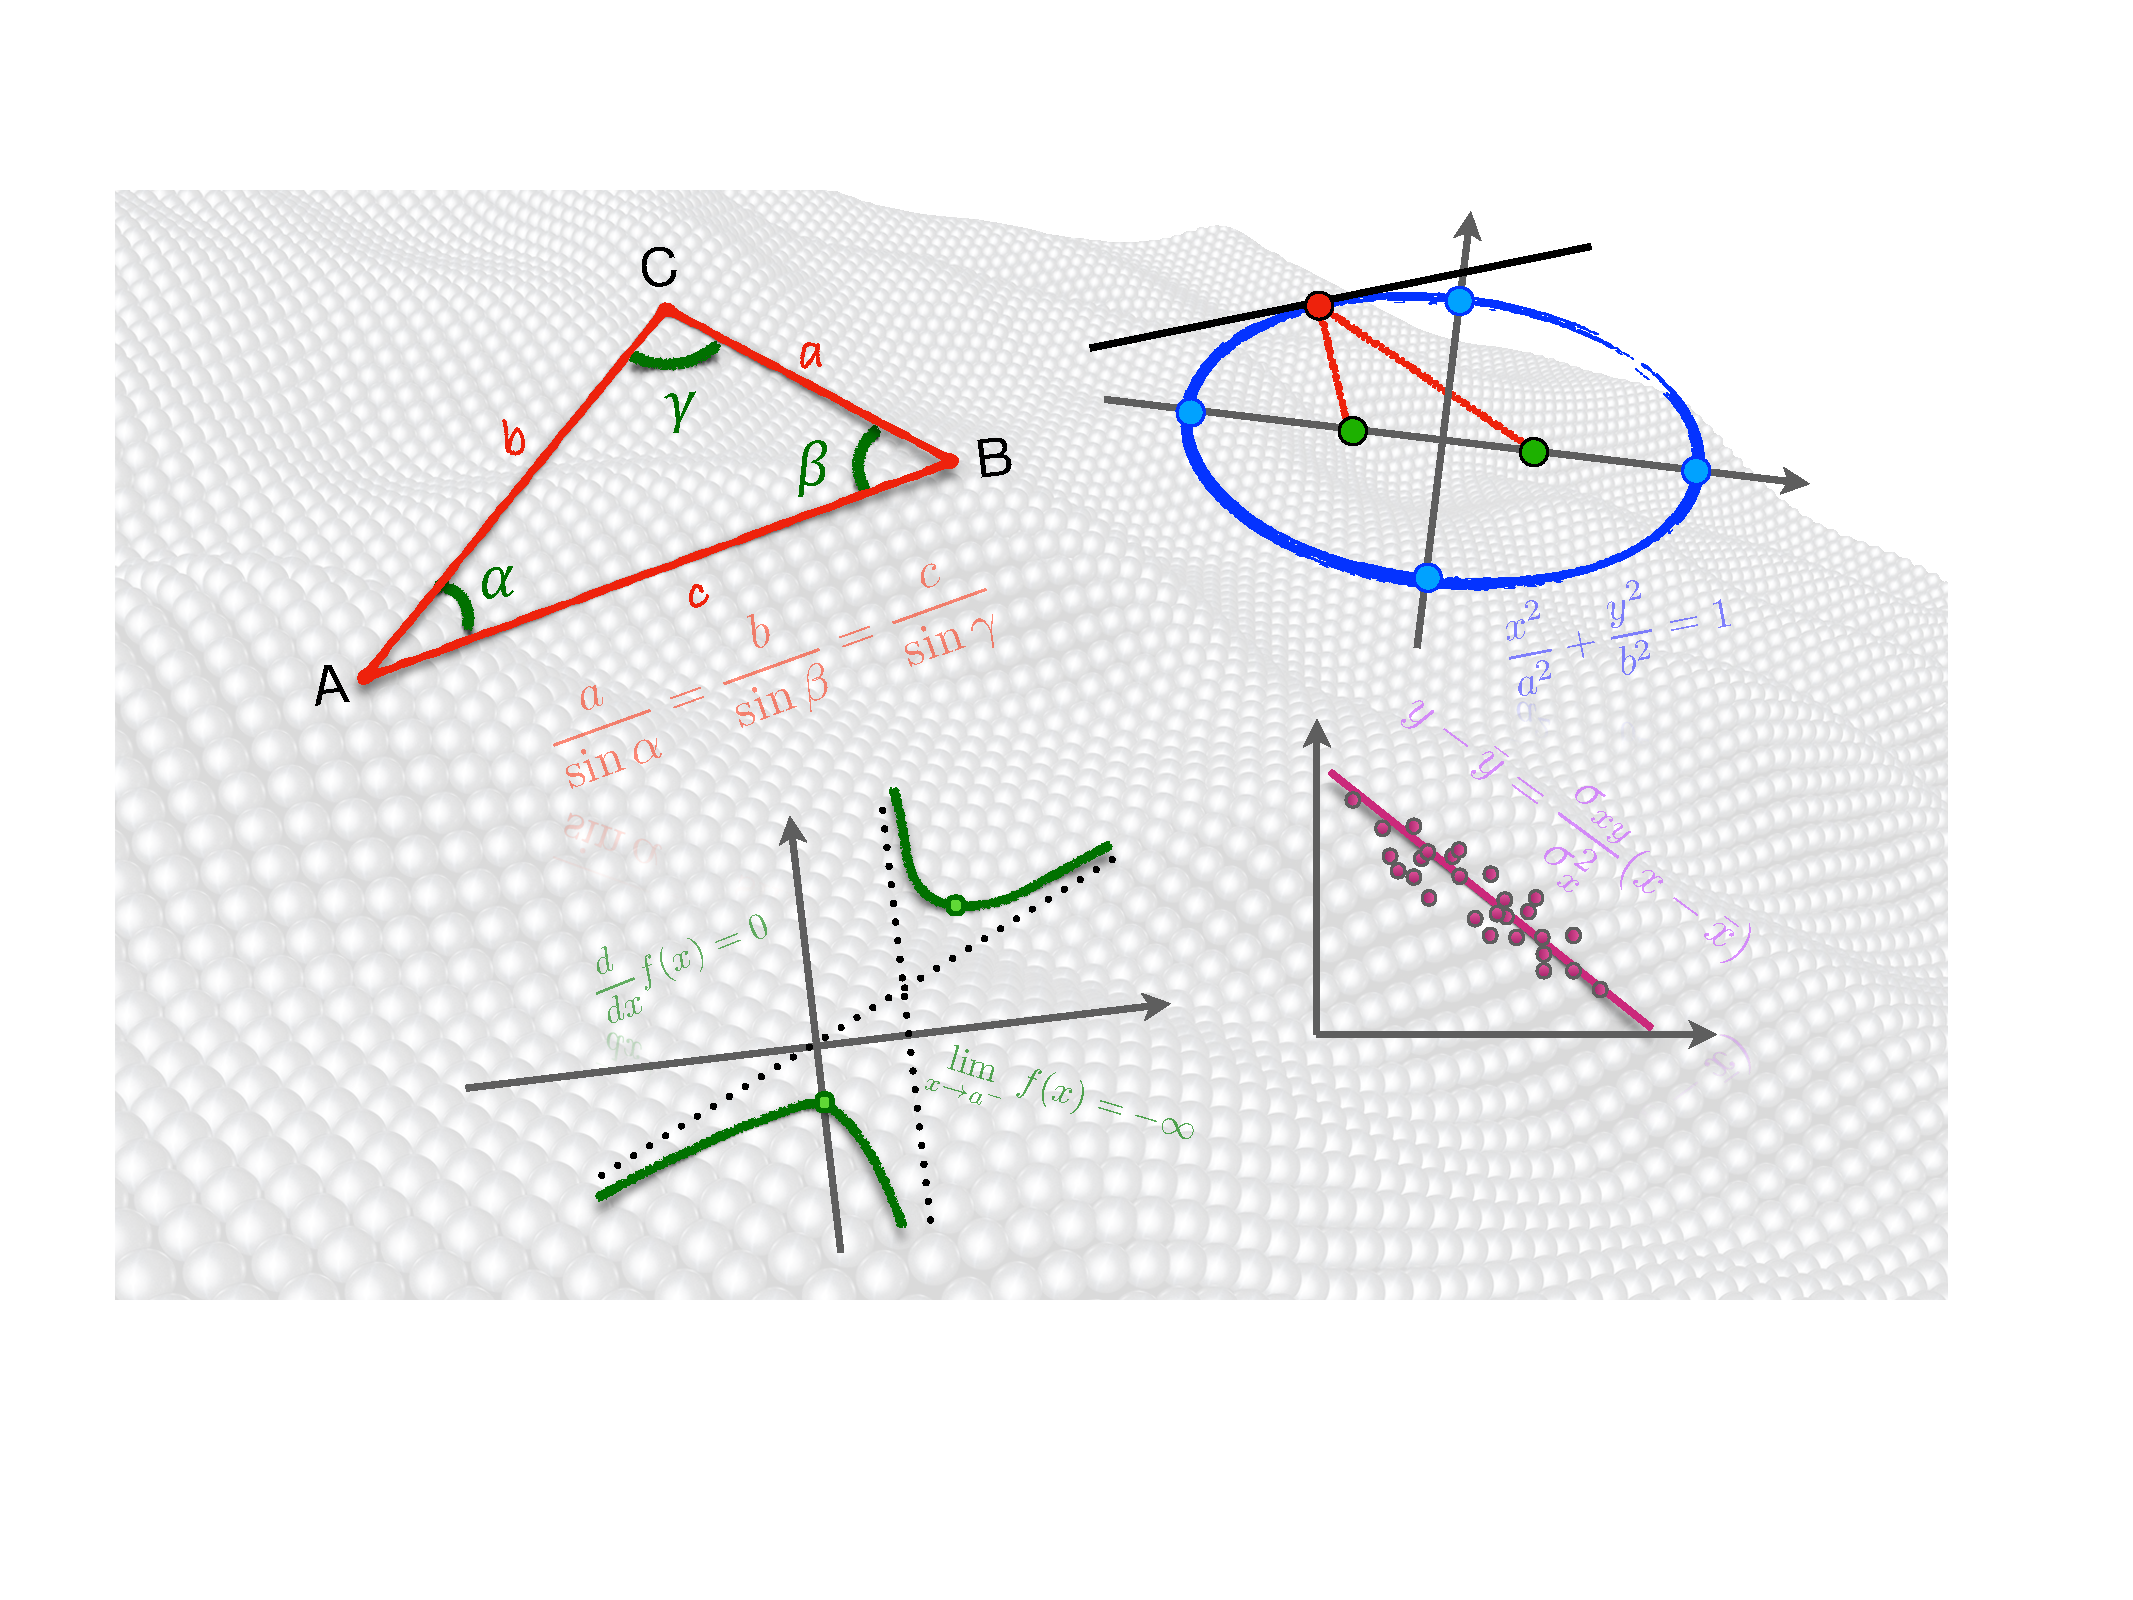
\includegraphics[width=0.9\textwidth]{img-00/portada}
	
	\vspace{1.5cm}
	
	
	\begin{minipage}{0.4\textwidth}
		\begin{center}
			\includegraphics*[width=1.2in]{img-00/ies-binissalem-logo}
			
			\small
			
			\noindent \href{www.iesbinissalem.net}{\textbf{www.iesbinissalem.net}}  
			
		\end{center}
	\end{minipage}
	\begin{minipage}{0.4\textwidth}
		\begin{flushright}
			\textbf{Josep Mulet}
			
			\textit{Departament de Matemàtiques} 
			
			IES Binissalem
		\end{flushright}
	\end{minipage} 
	
	
\end{center}

\newpage

\vspace*{12.9cm}
\begin{center}
	\begin{minipage}{0.5\textwidth}
		Aquesta és una obra derivada de ``\textit{Matematicas 1º de Bachillerato de ciencias. Ejercicios y problemas}'' de Marea Verde de matemàtiques. Per tant, està subjecta a les mateixes condicions de llicència CREATIVE COMMONS que l'obra original.
		
		\noindent \textbf{Edició \LaTeX: \quad \textregistered \,  Josep Mulet Pol}
		
		\noindent \textbf{Versió}: \quad 2018-06-29
		
		\noindent \textbf{Portada}: \quad \textit{Fractal de Julia}.
		
		
		\begin{center}
			\includegraphics*[width=8cm]{img-00/licencia}
		\end{center}
	\end{minipage}
\end{center}

%\clearemptydoublepage
%%\setcounter{page}{1}
%%\fancyfoot[C]{\roman{\thepage}}%


\newpage


\renewcommand{\thepage}{\Roman{page}}% Roman numerals for page counter
\pagestyle{myheadings}
\thispagestyle{empty}
\renewcommand{\headrulewidth}{0pt}
\renewcommand{\footrulewidth}{0pt}

\pagebreak


\dominitoc

\tableofcontents


\newpage

\heading{Currículum LOMCE}

\quad {\footnotesize Extret de \url{http://weib.caib.es/Normativa/Curriculum\_IB/batxillerat\_lomce/matematiques_batx.pdf} }

\begin{center}
	\fontsize{10.1}{13}\selectfont
	\leftmargin=0pt \itemindent=0pt 
	\begin{tabular}{|p{0.5\textwidth}|p{0.5\textwidth}|} \hline
		
		\rowcolor{lightgray} \textbf{BLOC: Nombres i Àlgebra} & \textbf{BLOC: Geometria} \\ \hline
		
		
		\begin{itemize}
			
			\item Nombres reals: necessitat del seu estudi per a la comprensió de la realitat. 
			
			\item Valor absolut. Desigualtats. Distàncies en la recta real. Intervals i entorns. 
			
			\item Aproximació i errors. Notació científica.
			
			\item Nombres complexos. Forma binomial i polar. Representacions gràfiques. Operacions elementals. Fórmula de Moivre.
			
			\item Successions numèriques: terme general, monotonia i acotació. El nombre e.
			
			\item Logaritmes decimals i neperians. Equacions logarítmiques i exponencials.
			
			\item Plantejament i resolució de problemes de la vida quotidiana mitjançant equacions i inequacions. Interpretació gràfica.
			
			\item Resolució d’equacions no algebraiques senzilles.
			Mètode de Gauss per a la resolució i interpretació de sistemes d’equacions lineals.
		\end{itemize}
		
		&
		
		\begin{itemize}
			
			\item 	Mesura d’un angle en radiants.
			
			\item Raons trigonomètriques d’un angle qualsevol. Raons trigonomètriques dels angles suma i diferència d’altres dos, doble i meitat. Fórmules de  transformacions trigonomètriques.
			
			\item Teoremes. Resolució d’equacions trigonomètriques senzilles.
			
			\item Resolució de triangles. Resolució de problemes geomètrics diversos.
			
			\item Vectors lliures en el pla. Operacions geomètriques.
			
			\item Producte escalar. Mòdul d’un vector. Angle de dos vectors.
			
			\item Bases ortogonals i ortonormals.
			
			\item Geometria mètrica plana. Equacions de la recta. Posicions relatives de rectes. Distàncies i angles. Resolució de problemes.
			
			\item Llocs geomètrics en el pla.
			
			\item Còniques. Circumferència, el·lipse, hipèrbola i paràbola. Equació i elements.
			
			
		\end{itemize}
		\\ \hline
		
		\rowcolor{lightgray}  \textbf{BLOC: Anàlisi} & \textbf{BLOC: Estadística i probabilitat}  \\ \hline
		
		\begin{itemize}
			
			\item 	Funcions reals de variable real.
			
			\item Funcions elementals: polinòmiques, racionals senzilles, valor absolut, arrel, trigonomètriques i les seves inverses, exponencials, logarítmiques i funcions definides a trossos.
			
			\item Operacions i composició de funcions. Funció inversa. Funcions d’oferta i demanda.
			
			\item Concepte de límit d’una funció en un punt i en l’infinit. Càlcul de límits. Límits laterals. Indeterminacions.
			
			\item Continuïtat d’una funció. Estudi de discontinuïtats.
			
			\item Derivada d’una funció en un punt. Interpretació geomètrica de la derivada de la funció en un punt. Recta tangent i normal.
			
			\item Funció derivada. Càlcul de funcions derivades. Regla de la cadena.
			
			\item Representació gràfica de funcions.
			
		\end{itemize}		
		&
		
		\begin{itemize}
			\item 	Estadística descriptiva bidimensional:
			Taules de contingència.
			
			\item Distribució conjunta i distribucions marginals.
			
			\item Mitjanes i desviacions típiques marginals.
			
			\item Distribucions condicionades.
			
			\item Independència de variables estadístiques.
			
			\item Estudi de la dependència de dues variables estadístiques. 
			
			\item Representació gràfica: Núvol de punts.
			
			\item Dependència lineal de dues variables estadístiques. 
			
			\item Covariància i correlació: Càlcul i interpretació del coeficient de correlació lineal.
			
			\item Regressió lineal. Estimació. Prediccions estadístiques i fiabilitat de les mateixes.
		\end{itemize}		
		\\ \hline
		
		
	\end{tabular}	
\end{center}

\cleartorightpage
 

\vspace*{2cm} 
\heading{Símbols}

\begin{center}
	\renewcommand{\arraystretch}{1.5}
	\begin{longtable}[h]{>{\raggedleft\arraybackslash}p{0.19\textwidth}|p{0.78\textwidth}}
		{\bfseries Símbol} & {\bfseries Significat} \\ \hline
		
		\simbolclau & Problema clau amb solució al final del llibre.  \\ \hline
		
		\simbolcompass & A més de la solució, proporciona orientacions per arribar a ella.  \\ \hline
		
		\simbolsearch & Problema que requereix d'investigació o recerca d'informació.  \\ \hline
		
		\ggb & Activitat adequada per realitzar amb el programa Geogebra.  \\ \hline
		
		\begin{center}
\includegraphics[width=1cm]{img-00/video-164}\par {\footnotesize Vídeo 132:}\end{center} & Explicació en vídeo dels continguts de l'apartat. El número de vídeo correspon a la numeració emprada en https://piworld.es 
		
		\\ \hline
		\hot[2] & Problema amb un cert grau de dificultat. \\ [0.25cm] \hline
		\spen & Activitat que es pot contestar en el llibre mateix. \\ [0.25cm] \hline 
		\mental & Activitat que es pot resoldre mentalment o en veu alta.
	\end{longtable}
\end{center}
\vspace{1cm} 

\heading{Recursos}

\begin{center}
	\renewcommand{\arraystretch}{1.5}
	\begin{longtable}[h]{>{\raggedleft\arraybackslash}p{0.2\textwidth}|p{0.8\textwidth}}
		\hline
		\textbf{piWorld}
		
		
\includegraphics[height=1.5cm]{img-00/piworld}
		& Plataforma d'aprenentatge. Conté explicacions en vídeo i activitats interactives. Requereix usuari i contrasenya. \newline
		\quad \href{https://piworld.es}{\href{https://piworld.es}{https://piworld.es}}
		\\ \hline
		\textbf{Geogebra} 
		
		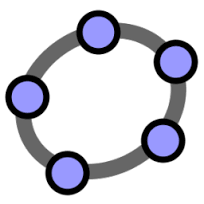
\includegraphics[height=1.5cm]{img-00/geogebra}
		& Programa lliure de geometria dinàmica en dues i tres dimensions.
		Ideal pels temes de funcions i geometria.\newline
		\quad  \href{https://www.geogebra.org/download}{\href{https://www.geogebra.org/graphing}{https://www.geogebra.org/graphing}}
		\\ \hline
		\textbf{Calculadora WIRIS}
		
		
		
\includegraphics[height=2cm]{img-00/wiris}
		& Calculadora per al càlcul simbòlic. Nova versió Web \par \quad  \href{https://calcme.com/a}{https://calcme.com/a}
		
		La versió antiga la trobareu a \par \quad  \href{http://www.wiris.net/educa.madrid.org/wiris/es/cas.html}{http://www.wiris.net/educa.madrid.org/wiris/es/cas.html}
		
		Atenció: requereix el plugin de Java i no funciona en dispositius mòbils.
		\\ \hline
		
	\end{longtable}
\end{center}



\pagestyle{fancy}

 
  
\mypart[Fractal de Mandelbrot. La bellesa dels nombres complexos.]{ARITMÈTICA, ÀLGEBRA I TRIGONOMETRIA}{img-00/bloc1}

\vspace*{\fill}
\begin{center}
	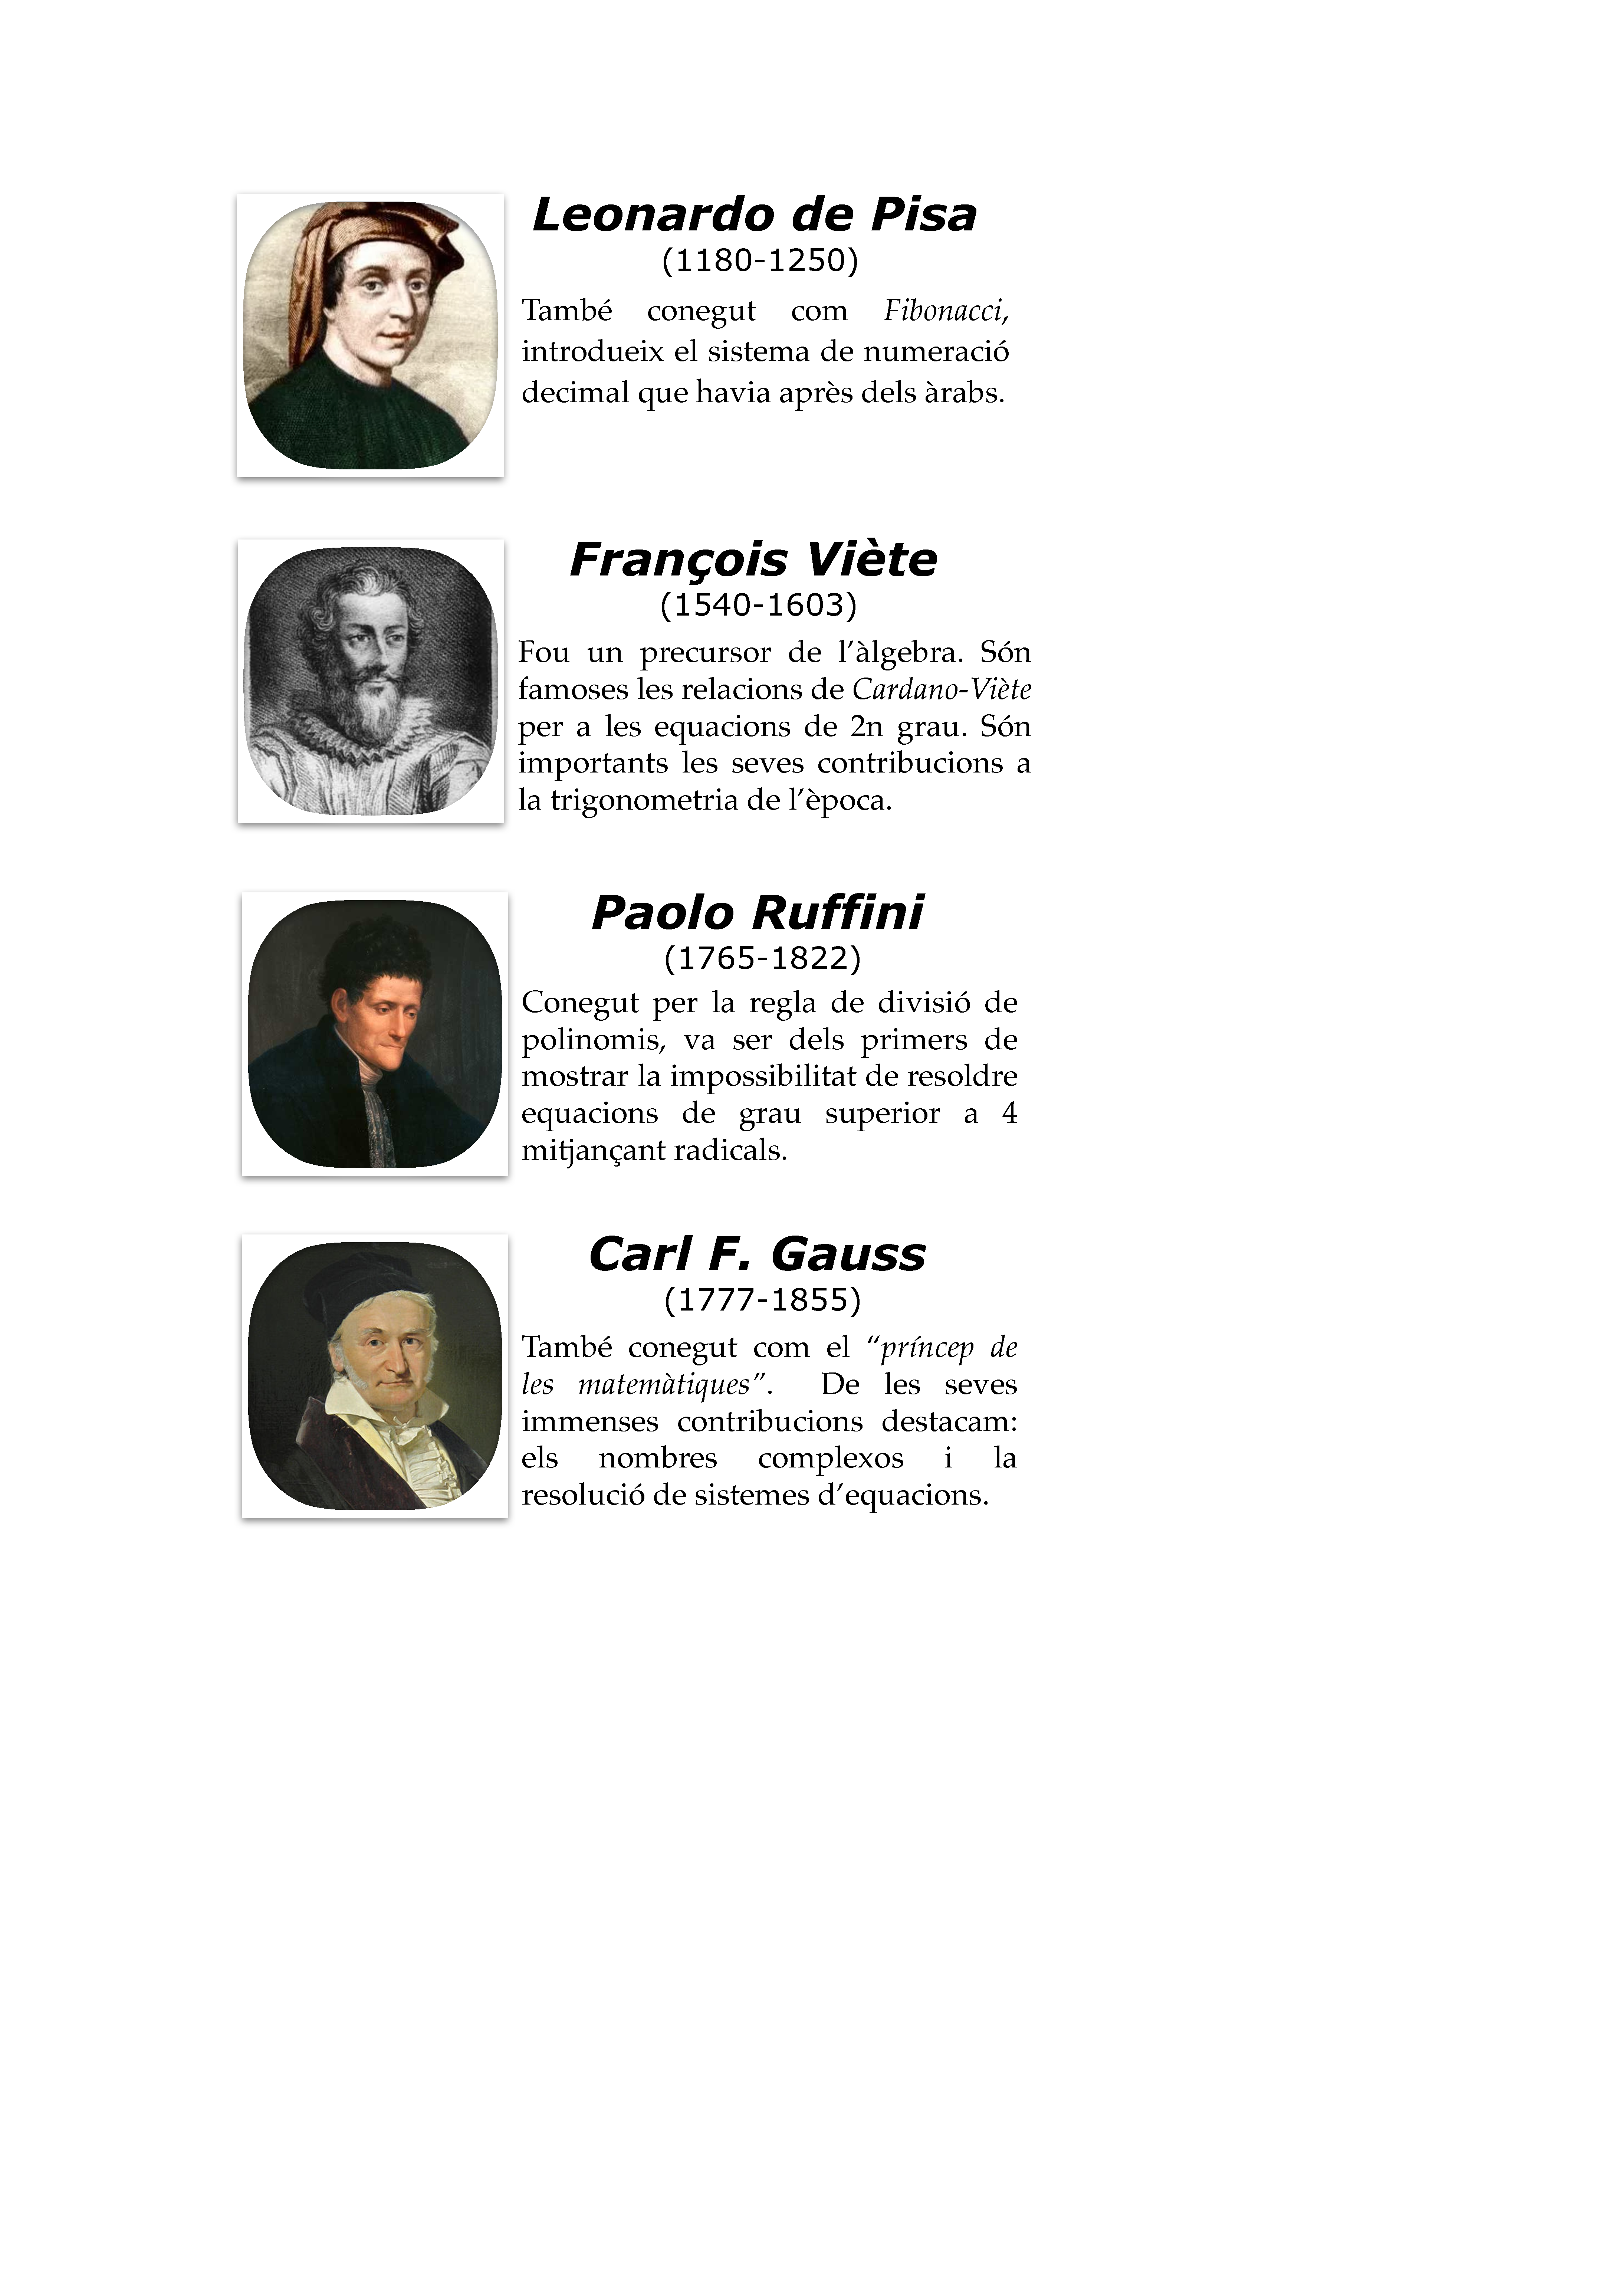
\includegraphics[width=0.65\textwidth]{img-00/bloc1-historia}
\end{center}
\vspace*{\fill}

\mychapter{Nombres reals}{Nombres reals}{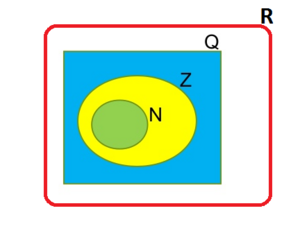
\includegraphics[width=4cm]{img-01/chap1.png}}
{chap:real}
 
\section{La recta real}

\begin{tip}
	Els nombres reals es classifiquen en: Naturals $\mathbb{N}=\{1,2,3,\cdots \}$, \par Enters $\mathbb{Z}=\{\cdots,-2,-1, 0, 1,2,\cdots \}$, Racionals $\mathbb{Q}=\{\frac{a}{b},\, a $ i $ b\neq 0 $ enters $  \}$, \par Irracionals $\mathbb{I}=\{\sqrt{2}, \pi, e, \cdots \}$ i els nombres reals  $\mathbb{R}=\mathbb{Q}\cup \mathbb{I}$.\par
		\rule{\textwidth}{1pt}
		
	El \textbf{valor absolut} d'un nombre és $|a|=a$ si $a\geq 0$, $|a|=-a$ si $a<0$.
	
	La \textbf{distància} entre dos nombres es troba mitjançant $\mathrm{Dist}(a,b)=|b-a|$. 

\end{tip}

\begin{mylist}
  
	\exer \spen
		 Troba l'expressió decimal de les fraccions
		\begin{tasks}(3)
			\task $\dfrac{2}{3}=$
			\task $\dfrac{3}{4}=$
			\task $\dfrac{7}{30}=$
			\task $\dfrac{6}{25}=$
			\task $\dfrac{7}{8}=$
			\task $\dfrac{9}{11}=$	
		\end{tasks} 
	\answers{[$0.\hat 6$, $0.75$, $0.2\hat 3$, $0.24$, $0.875$, $0.\widehat{81}$]}

	\exer  Escriu en forma de fracció les següents expressions decimals periòdiques, redueix-les i comprova que està bé:
	\begin{tasks}(4)
		\task $2,353535{\cdots}$
		\task $87,23656565{\cdots}$
		\task $0,9999{\cdots}$
		\task $26,5735735735{\cdots}$
	\end{tasks} 
\answers{[$233/99$, $431821/3300$, $1$]}
  	
    \pagebreak
	\exer  Representa a la recta numèrica els següents nombres racionals:
	\begin{tasks}(4)
		\task $\dfrac{9}{5} $
		\task $\dfrac{-13}{4} $
		\task 1,342
		\task $-$2,555555{\dots}
	\end{tasks} 


	\exer  Representa a la recta numèrica els nombres irracionals:
	\begin{tasks}(4)
		\task $\sqrt{10} $
		\task  $-\sqrt{6} $
		\task $\sqrt{27} $
		\task 	$\dfrac{1+\sqrt{5} }{2} $ 
	\end{tasks}
 
	\exer \spen Escriu el valor absolut dels següents nombres: 
	\begin{tasks}(3)
		\task $|5|=$
		\task $|-5|=$
		\task $|\pi-\sqrt{10}|=$
	\end{tasks}
\answers[cols=3]{[5, 5, $\sqrt{10}-\pi$]}
 

	\exer  Representa a la recta real i calcula la distància entre els nombres reals següents: 
	\begin{tasks}(2)
		\task Dist(5 , 9) 
		\task Dist($-$2.3 , $-$4.5)
		\task Dist($-$1/5 , 9/5)
		\task Dist($-$3.272727{\dots}. ,  6.27272727{\dots}.)
	\end{tasks}
\answers{[4, 2.2, 2, 9]}
  
	
\section{Intervals i entorns}
	
	\exer  Escriu els següents intervals mitjançant conjunts i representa'ls a la recta real:
	\begin{tasks}(4)
		\task $[1, 7)$ 
		\task $(-3, 5)$
		\task $(2, 8]$ 
		\task ($-\infty$, 6)
	\end{tasks}
\answers{[$1\leq x<7$, $-3<x<5$, $2<x\leq8$, $x<6$]}
 


	\exer  Representa a la recta real i escriu en forma d'interval:
	\begin{tasks}(4)
		\task  $2 < x < 5$
		\task  $4 < x$
		\task $3 \leq x < 6$
		\task 	$x \leq 7$
	\end{tasks}
\answers{[$(2,5)$, $(4,+\infty)$, $[3,6)$, $(-\infty,7]$]}

 

	\exer \spen Expressa com a interval o semirecta, en forma de conjunt (emprant desigualtats) i representa'ls gràficament:
	
	   \begin{tasks}
	   	\task  Un percentatge superior al 26 \% \dotfill
		%
		\task  Edat inferior o igual a 18 anys \dotfill
		%
		\task  Nombres, el cub dels quals, sigui superior a 8 \dotfill
		%
		\task  Nombres positius la part entera dels quals té 3 xifres \dotfill
		%
		\task  Temperatura inferior a 25 ºC \dotfill
		%
		\task  Nombres pels quals existeix la seva arrel quadrada  \dotfill
		%
		\task  Nombres que estiguin de 5 a una distància inferior a 4 \dotfill
	\end{tasks}
\answers{[$(26,100]$, $[0,18]$, $(2,+\infty)$, $[100,1000)$, $(-\infty,25)$, $[0,+\infty)$, $(1,9)$]}

\end{mylist}
\begin{theorybox}[Entorn obert]
	Es defineix l'entorn obert de centre $a$ i radi $r$, i s'escriu $E(a,\, r)$, com l'interval $(a-r, a+r)$ 
\end{theorybox}

\begin{resolt}{
	Expressa l'interval $(-1,5)$ com un entorn. }
	
	El centre es troba al punt mitjà $a=2$ i el radi és $r=3$, és a dir $(-1,5)=E(2,\, 3)$
\end{resolt}

 
\begin{mylist}
 
	\exer  Expressa en forma d'interval els següents entorns:
	\begin{tasks}(3)
		\task \textit{E}(1, 5)
		\task \textit{E}($-2$, $\frac{8}{3} $ )
		\task \textit{E}($-10$, $0.001$)
	\end{tasks}
\answers{[$(-4,6)$, $(-14/3,2/3)$, $(-10.001,-9.999)$]}
 
 
	\exer  Expressa en forma d'entorn els següents intervals:
	\begin{tasks}(3)
		\task $(4,\, 7)$
		\task $(-7,\, -4)$
		\task $(-3,\, 2)$
	\end{tasks}
\answers{[$(5.5,1.5)$, $(-5.5,1.5)$, $(-0.5,2.5)$]}
 

\exer Calcula $x$ en les següents equacions: (pista: $x$ pot tenir dos valors)
\begin{tasks}(3)
	\task $|x|=5$
	\task $|x-4|=0$
	\task $|3x+9|=21$
\end{tasks}
\answers{[$x=$ 5 i --5, $x=$ 4, $x=$ --10 i 4]}
 


\exer Representa a la recta real els nombres que verifiquen les següents relacions:
\begin{tasks}(4)
	\task $|x|<1$
	\task $|x|\leq 1$
	\task $|x-3|>1$
	\task $|x-3|\geq 1$
\end{tasks}
\answers[cols=1]{[$(-1,1)$, $(-\infty,-1]\cup [1,+\infty]$, $(-\infty,2)\cup(4,+\infty)$, $(-\infty,2]\cup[4,+\infty)$]}


\exer Troba dos nombres que distin 6 unitats de 3, i altres dos que distin 3,5 unitats de $-$2, calcula després la diferència entre el major i el menor de tots aquests nombres. 
\answers{$-3$ i $9$. $-5.5$ i $1.5$. $9-(-5.5)=14.5$}

\exer Escriu l'interval [$-$3, 5] $\mathrm{\cap}$ (3, 8).
\answers{$[-3, 8)$}
 
\exer Escriu l'interval format pels nombres reals x que compleixen $|x-8|\leq 3$. 
\answers{$[5,11]$}

\exer Determina els conjunts A $\mathrm{\cap}$  B, A  $\cup$ B, A $-$ B i $-$A en els casos següents:
\begin{tasks}(2)
	\task A = [\textit{$-$}11, \textit{$-$}9]; B = (\textit{$-$}1, 6)
	\task  A = [\textit{$-$}5, 5]; B = (3, 4)	
\end{tasks}
 \answers{[$A\cap B=\emptyset$;\par $A\cup B=[-11,-9] \cup (-1,6)$;\par $A-B=A$,  
 		   $A\cap B=B$; $A\cup B=A$;\par $A-B=[-5,3]\cup [4,5]$]}
 
\end{mylist}
 

\section{Radicals}

\begin{theorybox}
	Trobareu un resum de les propietats dels radicals a la pàgina \pageref{page:pradicals}.
\end{theorybox}

\begin{mylist}
	
\exer[1]  Expressa com un sol radical:
\begin{tasks}(3)
\task $\sqrt{\sqrt[{3}]{5} } =$          
\task $\sqrt[{4}]{\sqrt[{}]{8} } $=                   
\task $\sqrt{\sqrt{x^{3} \sqrt{x} } } $=
\end{tasks}
\answers[cols=3]{[$\sqrt[{6}]{5} $,  $\sqrt[{8}]{8} $,  $\sqrt[{8}]{x^{7} } $]}

\exer[1] Simplifica, extraient tots els factors que puguis del radical:
\begin{tasks}(4)
	\task  $\sqrt[{4}]{64} $=      
	\task  $\sqrt[{}]{243} $=          
	\task  $\sqrt[{9}]{216} $=      
	\task  $\sqrt[{8}]{1024} $=
	\task  $\sqrt[{15}]{243} $=   
	\task  $\sqrt[{6}]{2401} $= 
	\task  $\sqrt[{16}]{49} $=      
	\task  $\sqrt[{14}]{128} $=
\end{tasks}
\answers{[$2\,\sqrt[{}]{2} $,   $9\,\sqrt[{}]{3} $,     $\sqrt[{3}]{6} $,    $2\,\sqrt[{4}]{2} $,  $\sqrt[{3}]{3} $,     $\sqrt[{3}]{49} $,       $\sqrt[{8}]{7} $,   $\sqrt{2} $]}

\exer[1] Redueix el radical a l'\'{i}ndex indicat:
\begin{tasks}(4)
	\task $\sqrt[{4}]{2^{3} } =\sqrt[{12}]{2^{\_ \_ } } $    
	\task $\sqrt{7} =\sqrt[{16}]{7^{\_ \_ } } $    
	\task $\sqrt[{4}]{a^{6} } =\sqrt{a^{\_ \_ } } $     
	\task $\sqrt[{6}]{5^{12} } =\sqrt[{3}]{5^{\_ \_ \_ } } $
\end{tasks}
\answers{[$\sqrt[{4}]{2^{3} } =\sqrt[{12}]{2^{9} } $,       $\sqrt{7} =\sqrt[{16}]{7^{8} } $,    $\sqrt[{4}]{a^{6} } =\sqrt{a^{3} } $,     $\sqrt[{6}]{5^{12} } =\sqrt[{3}]{5^{6} } =5^{2} $]}

\exer[1] Expressa com un sol radical (redueix, primer de tot, els radicals a \'{i}ndex com\'{u} i simplifica si pots):  
\begin{tasks}(2)
	\task $\dfrac{\sqrt[{6}]{32} \, \cdot \, \sqrt[{3}]{25} \, }{\sqrt{8} } $   
	\task $\dfrac{\sqrt{2} \, \cdot \, \sqrt[{3}]{3} }{\sqrt[{4}]{6} } $   
	\task $\dfrac{\sqrt{5} \, \cdot \, \sqrt[{3}]{5} }{\sqrt[{4}]{5} } $     
	\task $\sqrt{\sqrt{\sqrt{2^{24} } } } $
	\task $\left(\sqrt[{5}]{64} \right)^{4} $   
	\task $\sqrt[{3}]{\sqrt{\sqrt[{3}]{5^{9} } } } $   
	\task $\sqrt{3\, \sqrt{3\, \sqrt{3^{2} } } } $    
	\task $\left(\sqrt{\sqrt[{3}]{125} } \right)^{4} $
\end{tasks}
\answers[cols=2]{[$\sqrt[{3}]{5/4} $,      $\sqrt[{12}]{2^{3} \cdot 3} $,  $\sqrt[{12}]{5^{7} } $,   $2^{3} $,      $2^{4} \cdot \sqrt[{5}]{2^{4} } $,     $\sqrt[{}]{5} $,      3,       $5^{2} $]}

\begin{example}
	a) $\dfrac{\sqrt[{6}]{32} \, \cdot \, \sqrt[{3}]{25} \, }{\sqrt{8} } =     \dfrac{\sqrt[{6}]{32} \, \cdot \, \sqrt[{6}]{25^2} \, }{\sqrt[6]{8^3} } =
	\sqrt[6]{\dfrac{2^5 \, \cdot \, 5^4 \, }{2^9 }} = \sqrt[6]{\dfrac{  5^4 \, }{2^4 }} =\sqrt[3]{\left(\dfrac{  5 }{2 }\right)^2 }
	$ 
\end{example}

\exer[1] Calcula, extraient primer factors fora dels radicals:
\begin{tasks}(2)
	\task $\sqrt{1331} $ - $\sqrt{44} $ + 2 $\sqrt{99} $=  
	\task $\sqrt[{3}]{16} $ + $\sqrt[{3}]{686} $ - 3 $\sqrt[{3}]{2} $= 
	\task 2 $\sqrt{54} $ - $\sqrt{216} $ - $\sqrt{\frac{6}{25} } $= 
	\task $\sqrt[{4}]{32} $ + $\sqrt[{4}]{\frac{2}{81} } $ - 7 $\sqrt[{4}]{2} $=
	\task 2 $\sqrt{3} $ - $\frac{1}{5} $ $\sqrt{27} $ + $\frac{2}{3} $ $\sqrt{12} $= 
	\task $\sqrt{32} $ - $\sqrt{18} $ + $\frac{1}{5} $ $\sqrt{128} $=
\end{tasks}
\answers{[
		$15\,\sqrt[{}]{11} $,  $6\,\sqrt[{3}]{2} $,      $-\sqrt[{}]{6} /5$,    $-14\,\sqrt[{4}]{2} /3$,    $41\,\sqrt[{}]{3} /15$,    $13\,\sqrt[{}]{2} /5$]}

   \begin{example}
	a) $\sqrt{1331} - \sqrt{44}  + 2 \sqrt{99} = \sqrt{11^3}  - \sqrt{2^2\cdot 11}  + 2 \sqrt{3^2 \cdot 11} =$ 
	
	\qquad\qquad\qquad\qquad\qquad\qquad = $11\sqrt{11}  - 2\sqrt{11}  + 2\cdot 3 \sqrt{11}= 15\sqrt{11}$ 
	\vspace{0.25cm} 
\end{example}

\exer[1] Desenvolupa $\left(1+\left(1+\sqrt{a} \right)^{2} \right)^{2} =$
\answers{$(2+a)^{2} +4(2+a)\sqrt{a} +4a$}

\exer[1] Racionalitza:
\begin{tasks}(3)
	\task $\dfrac{1}{\sqrt[{3}]{3} } $ =     
	\task $\dfrac{3}{2\, \sqrt[{4}]{2} } $=        
	\task $\dfrac{3}{\sqrt{2} -1} $=
	\task $\dfrac{\sqrt{2} +1}{\sqrt{2} -1} $   
	\task $\dfrac{\sqrt{2} }{\sqrt{5} +\sqrt{3} } $=    
	\task $\dfrac{2+\sqrt{5} }{2-\sqrt{5} } $=
\end{tasks}
\answers[cols=2]{[$\frac{\sqrt[{3}]{3^{2} } }{3} $, $\frac{3}{4} \,\sqrt[{4}]{2^{3} }$,  $3(\sqrt{2+1} )$,   $3+2\sqrt{2} $,    $(\sqrt{10} -\sqrt{6} )/2$,    $-(9+4\sqrt{5} )$]}

\begin{example}
	d)  $\dfrac{\sqrt{2} +1}{\sqrt{2} -1} = \dfrac{(\sqrt{2} +1)}{(\sqrt{2} -1)} \cdot \dfrac{(\sqrt{2} +1)}{(\sqrt{2} +1)} = \dfrac{(\sqrt{2} +1)^2}{(\sqrt{2})^2 -1^2}=3+2\sqrt{2}$   
\end{example}
 
\exer[1] Opera, racionalitza i simplifica
\begin{tasks}(2)
	\task $\dfrac{\sqrt{48} }{\frac{\sqrt{8} }{3} } =$  
	\task $\dfrac{\sqrt[{4}]{2} }{\frac{2}{\sqrt{2} } } =$ 
	\task $\dfrac{\frac{1}{2} }{\frac{\sqrt{3} }{3} } =$        
	\task  ${\rm (4}\sqrt{{\rm 5}} +{\rm 3}\sqrt{{\rm 5}} {\rm )}\, {\rm \cdot }\, {\rm (4}\sqrt{{\rm 5}} -{\rm 3}\sqrt{{\rm 5}} {\rm )}$=  
	\task ${\rm 2}^{-{\rm 5}} \, {\rm \cdot }\, {\rm 2}^{\frac{{\rm 1}}{{\rm 3}} } \, {\rm \cdot }\, \sqrt{{\rm 2}^{{\rm 5}} } =$
	\task $\left(\frac{{\rm 5}}{{\rm 2}} -\sqrt{{\rm 2}} \right)^{{\rm 2}} =$ 
%	\task $\dfrac{\frac{1}{2} +\frac{3}{7} }{2-\frac{4}{6} } =$    
\end{tasks}
\answers[cols=2]{[$3\sqrt{6}$,     $\frac{\sqrt[{4}]{2^{3} } }{2} $,    $\frac{\sqrt{3} }{2} $,     35,    $2^{-64/15} $,    $33/4-5\sqrt{2} $]}

\end{mylist}

\pagebreak






\begin{autoaval}{21}

\begin{mylist}
	
	\exer[2] Resol l'equació $|3x+9|=21$.
	\begin{comment}
	\begin{tasks}(4)
	\task $x=10$, $x=-4$
	\task $x=10$ 
	\task $x=-10$, $x=4$
	\task $x=-4$
	\end{tasks}
	\end{comment}
	\answers{$x=-10$ i $x=4$}		
			
	\exer[2] Expressa $\sqrt[4]{x\sqrt{x}}$ com una única arrel.
	\begin{comment}
	\begin{tasks}(4)
		\task $\sqrt[4]{x^2}$
		\task $\sqrt[8]{x^2}$
		\task $\sqrt[8]{x^3}$
		\task $\sqrt{x^{4}}$	
	\end{tasks}
	\end{comment}
	\answers{$\sqrt[8]{x^3}$}

	\exer[2] Simplifica l'expressió $(2\sqrt{3}+1)^2$.
	\begin{comment}
	\begin{tasks}(4)
	\task 7
	\task 13
	\task $7+4\sqrt{3}$
	\task $13+4\sqrt{3}$	
	\end{tasks}	
	\end{comment}
	\answers{$13+4\sqrt{3}$}
	


	\exer[2] Racionalitza l'expressió $\dfrac{4}{\sqrt{5}}$.
	\begin{comment}
\begin{tasks}(4)
\task $\dfrac{4\sqrt{5}}{5}$ 
\task $4\sqrt{5}$ 
\task $20 \sqrt{5}$ 
\task $\dfrac{20\sqrt{5}}{4}$ 
\end{tasks}	
	\end{comment}
\answers{$\dfrac{4\sqrt{5}}{5}$}


	\exer[2] Simplifica l'expressió $\sqrt[3]{54} + \frac{2}{3}\sqrt[3]{16}$.
	\begin{comment}
\begin{tasks}(4)
\task $\frac{5}{3}\sqrt[3]{70}$
\task $\frac{5}{3}\sqrt[3]{70}$
\task $\frac{13}{3}\sqrt[3]{2}$
\task $13\sqrt[3]{2/3}$	
\end{tasks}	
	\end{comment}
\answers{$\frac{13}{3}\sqrt[3]{2}$}


	\exer[2] Racionalitza l'expressió $\dfrac{2\sqrt{5}-\sqrt{3}}{\sqrt{5}+2\sqrt{3}}$.
\answers{$\dfrac{16-5\sqrt{15}}{-7}$}
 

	\exer[2] Donats els intervals $A=[-11,6]$ i $B=(-1,9)$, calcula $A\cap B$.
	\begin{comment}
\begin{tasks}(4)
\task $(-11,9)$
\task $[-11,9)$
\task $(-1,9)$
\task $(-1,6]$	
\end{tasks}	
	\end{comment}
\answers{$(-1,\,6]$}
 
\end{mylist}

\vspace{1cm}

\end{autoaval}
 
 
\resum

\begin{center}
	\setlength\LTleft{0pt}
	\setlength\LTright{0pt}
	\ftimes{10.5}{11}
	\fontsize{10.5}{11}
	\renewcommand{\arraystretch}{1.2}
	\begin{longtable}[h]{|>{\raggedleft\arraybackslash}p{0.19\linewidth}|p{0.77\linewidth}|}
		\toprule %inserts double horizontal lines
		\rowcolor{lightgray}
		
		\textbf{Apartat} & \textbf{Resum} \\   [0.5ex] 
		\toprule  \hline
		
		
		\cellcolor{lightgray}\noindent \textbf{Nombres reals}  &   Està format per la unió dels nombres racionals i els nombres irracionals
		
		\sample{
			5, $-$4,  2/3, 7.5, $\pi$, $e$, $\Phi$ ${\dots}$ 
		}
		\\   \hline
		
		
		\cellcolor{lightgray}\noindent \textbf{Valor absolut}  & 
		
		\begin{minipage}{5cm} $\left|x\right|=\left\{\begin{array}{cc} {-x} & {si\; x<0} \\ {x} & {si\, x\, \ge 0} \end{array}\right. $
		\end{minipage}
		 \examplebox{$|-32|=32$}
	 
	    \\   \hline 
		
		
		\cellcolor{lightgray}\noindent \textbf{Distància a la recta real}  &  
		Dist(\textit{x}, \textit{y}) = {\textbar}\textit{x} $-$ y{\textbar}
		\sample{
			Dist(3, 8) = {\textbar}8 $-$ 3{\textbar} = 5.\newline Dist($-$2, $-$9) = {\textbar}$-$9 $-$ ($-$2){\textbar} = {\textbar}$-$9 + 2){\textbar} = {\textbar}$-$7{\textbar} = 7
		}
		\\   \hline 
		
		
		\cellcolor{lightgray}\noindent \textbf{Intervals}  &  
		Obert : (\textit{a} \textit{, b}) = $\{$\textit{x}  $\in\Re$$\mid$ \textit{a} $<$  \textit{x} $<$ {b}$\}$\newline Tancat: [\textit{a} \textit{, b}] = $\{$\textit{x}  $\in\Re$$\mid$ \textit{a} $\leq$    \textit{x}$\leq$  {b}$\}$\newline Semiobert (esq):  (\textit{a} \textit{, b}] = $\{$\textit{x}   $\in\Re$$\mid$ \textit{a} $<$  \textit{x} $\leq$ {b}$\}$\newline Semiobert (dreta):  [\textit{a} \textit{, b}) = $\{$\textit{x}  $\in\Re$$\mid$ \textit{a} $\leq$  \textit{x} $<$ {b}$\}$  
		
		%\sample{
		%	(3, 5)\hspace{1cm} [3, 5]\hspace{1cm}  (2, 8]\hspace{1cm}  [1, 7) 
		%}
		\\   \hline
		\begin{comment}
		
		\cellcolor{lightgray}\noindent \textbf{Entorns}  &  
		Són una forma especial d'expressar els intervals oberts. Es defineix com el conjunt de nombres que estan a una distància de a  menor que \textit{r}: E(\textit{a , r}) 
		\sample{
			\textit{E}(2 , 4) = (2 $-$ 4 , 2 + 4) = ($-$2, 6) 
		}
		\\ \hline
		
		\end{comment}
		\cellcolor{lightgray}\noindent \textbf{Radicals}  &  
		Permeten donar solució a l'equació $x^n=a$ $\rightarrow$ $x=\sqrt[n]{a}=a^{1/n}$.
		Si $a>0$, l'arrel existeix sempre. Si $a<0$, només quan l'índex $n$ és senar.
		
		\sample{
			$x^3=8$  $\leftrightarrow$ $x=\sqrt[3]{8}=2$
		}
		\\   \hline
		
		\hline \bottomrule
	\end{longtable}
\end{center}
 
  
 
{\bfseries \large Propietats dels radicals}
\label{page:pradicals}


\begin{longtable}[h]{|>{\raggedright}p{0.47\textwidth}|p{0.47\textwidth}|}
	\hline %inserts double horizontal lines
	\rowcolor{lightgray}
	
	\textbf{Propietat} & \textbf{Exemple} \\   [0.5ex] 
   \hline
	
	
	\textbf{1. Producte d'igual índex}
	
	$\sqrt[n]{a} \cdot \sqrt[n]{b} = \sqrt[n]{a\cdot b}$
	&   $\sqrt{50} \cdot \sqrt{2} = \sqrt{100}=10$ \\ \hline
	\textbf{2. Quocient d'igual índex }
	
	$\dfrac{\sqrt[n]{a}}{\sqrt[n]{b}} = \sqrt[n]{\dfrac{a}{b}}$
	&   $\dfrac{\sqrt[3]{14}}{\sqrt[3]{7}} = \sqrt[3]{\dfrac{14}{7}}=\sqrt[3]{2}$ \\ \hline
	
	\textbf{3. Potència d'una arrel }
	
	$\left( \sqrt[n]{a} \right)^k = \sqrt[n]{a^k} $
	&   $\left( \sqrt[4]{5} \right)^3 = \sqrt[4]{5^3} $ \\ \hline
	
	\textbf{4. Arrel d'arrel }
	
	$\sqrt[m]{ \sqrt[n]{a} } = \sqrt[n\cdot m]{a} $
	
	&  $\sqrt[3]{ \sqrt[4]{5} } = \sqrt[12]{5} $ \\ \hline
	
	
	\textbf{5. Extreure factors }
	
	$\sqrt[]{a^2 \cdot b}  = a\sqrt[]{b}$, 
	$\sqrt[3]{a^3 \cdot b}  = a\sqrt[3]{b}$, 
	
	&  $\sqrt[]{ 18 } = \sqrt[]{3^2 \cdot 2} = 3 \sqrt{2} $
	
	$\sqrt[3]{ 7000 } = \sqrt[3]{10^3 \cdot 7} = 10 \sqrt [3]{7} $,     
	\\ \hline
	 
	\textbf{6. Introduir factors }
	
	Consisteix en el pas contrari que el pas [5]
	$a\, \sqrt[]{b} = \sqrt[]{a^2 \cdot b}$, \quad
	$a\, \sqrt[3]{b} =\sqrt[3]{a^3 \cdot b}$.
	
	&    
	\par
	
	$5\, \sqrt[]{3} = \sqrt[]{5^2 \cdot 3}=\sqrt{75}$
	
	$\sqrt{3\sqrt{x}}= \sqrt{\sqrt{3^2 \cdot x}}=\sqrt[4]{9x}$, 
	
	\\ \hline
	\textbf{7. Suma i resta. Simplificar expressions}
	
	El primer pas és factoritzar els radicands i després extreure factors. Finalment, podem sumar o restar arrels iguals
	
	&    
	
	\par
	
	$\sqrt[3]{54}+\sqrt[3]{16}+\sqrt[3]{81}=\sqrt[3]{3^3\cdot 2}+\sqrt[3]{2\cdot 2^3}+\sqrt[3]{3^3 \cdot 3}=3\sqrt[3]{2}+2\sqrt[3]{2}+3\sqrt[3]{3}=5\sqrt[3]{2}+3\sqrt[3]{3}$
	
	\\ \hline
	
\textbf{	8. Radicals equivalents }
	
	$\sqrt[n]{a} = \sqrt[n\cdot q]{a^q}$
	
	& 
	$\sqrt[3]{2}=\sqrt[6]{2^2}=\sqrt[9]{2^3}=\cdots$
	\\ \hline
	
	\textbf{9. Operacions amb diferent índex }
	
	Primer cal reduir els radicals a índex comú utilitzant la propietat [8]
	
	$\sqrt[n]{a} \cdot \sqrt[m]{b} = \sqrt[q]{a^{q/n} \cdot b^{q/m} }$
	
	essent $q=min.c.m(n, m)$
	
	& 
	
	$\sqrt[3]{2} \cdot \sqrt[4]{3} = \sqrt[12]{2^{4} \cdot 3^{3} }=\sqrt[12]{432}$
	
	\\ \hline
	\textbf{10. Racionalitzar I }
	
	$\dfrac{1}{\sqrt[n]{a^k}}=\dfrac{1}{\sqrt[n]{a^k}}\cdot 
	\dfrac{\sqrt[n]{a^{n-k}}}{\sqrt[n]{a^{n-k}}}=\dfrac{\sqrt[n]{a^{n-k}}}{a}$
	
	&   $\dfrac{2}{\sqrt[4]{5}}=\dfrac{2}{\sqrt[4]{5}}\cdot 
	\dfrac{\sqrt[4]{5^3}}{\sqrt[4]{5^3}}=\dfrac{2 \sqrt[4]{5^3}}{5}$  \\ \hline
	\textbf{11. Racionalitzar II} 
	
	Multiplicam i dividim pel conjugat del denominador
	
	$\dfrac{1}{(\sqrt{a}-\sqrt{b})}\cdot \dfrac{\sqrt{a}+\sqrt{b})}{(\sqrt{a}+\sqrt{b})}=
	\dfrac{\sqrt{a}+\sqrt{b}}{a-b}
	$
	
	&   
	$\dfrac{1}{(\sqrt{5}-\sqrt{2})}\cdot \dfrac{(\sqrt{5}+\sqrt{2})}{(\sqrt{5}+\sqrt{2})}=
	\dfrac{\sqrt{5}+\sqrt{2}}{3}$
	
	\\ \hline 
\end{longtable}

\mychapter{Àlgebra}{Àlgebra}{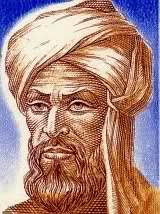
\includegraphics[width=3.1cm]{img-02/chap2.jpg}
	
	{\footnotesize Al Khwarizmi (780-850) }}
{chap:algebra}
 

\section{Operacions amb polinomis}
\vspace{-0.35cm}
\subsection{Identitats notables}
\vspace{-0.35cm}
\begin{theorybox}
	\begin{tabular}{ll}
	    \textbf{Quadrat d'una suma}: & $(a+b)^2 = a^2 + 2 ab+b^2$ \\
		\textbf{Quadrat d'una diferència}: & $(a-b)^2 = a^2 - 2 ab+b^2$\\
		\textbf{Suma per diferència}: & $(a+b)\cdot(a-b) = a^2 - b^2$ \\ [0.8ex]  
		\textbf{Quadrat d'un trinomi}: & $(a+b+c)^2 = a^2+b^2+c^2+2ab+2ac+2bc$		
	\end{tabular}
\end{theorybox}

\begin{mylist}
   
    	\exer  Desenvolupa les següents potències:
	    \begin{tasks}(3)
	      \task $\left(2{x} - 5{y}\right)^{2}$   
	      \task $\left(3{x} + \frac{y}{3}\right)^{2}$   
	      \task $\left(5^{2} - \frac{5}{x} \right)^{2}$
	       \task $\left(3{a} - {b}\right)^{2}$ 
	        \task $\left({a}^2 + {b}^{2}\right)^{2}$  
	         \task $\left(\frac{3y}{5} - \frac{2}{y}\right)^{2}$
	   \end{tasks}
   \answers[cols=1]{[$4x^2-20xy+25y^2$, $9x^2 +2xy+y^2/9$, $625-250+25/x^2$, $9a^2-6ab+b^2$, $a^4+2a^2b^2+b^4$, $9y^2/25 - 12/5+4/y^2$]}
   
    	\exer  Expressa com el quadrat d'una suma o d'una diferència les següents expressions algebraiques:
	    \begin{tasks}(3)
		   \task  $a^4 + 6a^2 + 9 $
		    \task  $9{x}^{2} - 6{x} + 1 $
		     \task  ${b}^{2} - 10{b} + 25$
		   \task  $4{y}^{2} + 12{y} + 9  $
		    \task  $a^4-2a^2+1$
		     \task  $y^{4} + 6{y}^{2} + 9$
	    \end{tasks}
    \answers[cols=1]{[$(a^2+3)^2$, $(3x-1)^2$, $(b-5)^2$, $(2y+3)^2$, $(a^2-1)^2$, $(y^2+3)^2$]}
   
   
   	\exer  Efectua aquests productes:
    \begin{tasks}(3)
     \task $(4x^{2} +3y)\cdot (4x^{2} -3y)$ \task $(2x^{2} +8)\cdot (2x^{2} -8)$  \task $(-x^{2} +3x)\cdot (x^{2} +3x)$
       \end{tasks}
   	\answers{[$16x^4-9y^2$, $4x^4-64$, $-x^4+9x^2$]}
\end{mylist}

 

\subsection{Divisió de polinomis}
\begin{theorybox}
	\begin{minipage}{0.7\textwidth}
		Per poder dividir $D(x):d(x)$ necessitam que el grau($D$)$\ge$grau($d$).
		
		\textbf{Comprovació}: Si dividim el dividend $D(x)$ entre el divisor $d(x)$, i obtenim el quocient $q(x)$ i el residu $r(x)$, s'ha de complir que 
		\begin{equation*}
		D(x) = q(x) \cdot d(x) + r(x)
		\end{equation*}
		
		Si $d(x)=x \pm a$ podem emprar la regla de \textbf{Ruffini}, sinó hem de fer la divisió en general.
	\end{minipage}
\hspace{0.5cm}
	\begin{minipage}{0.3\textwidth}
		\centering
		\videonw{46}{Divisió general}
		
		\videonw{47}{Divisió Ruffini}
	\end{minipage}
\end{theorybox}

\begin{resolt}[E]{
	\textbf{$(x^4+3x^3 - 4x+5):(x+2)$}
}

	Feim la divisió per la regla de Ruffini, recordant a posar 0 si falten potències de $x$.
	
	\begin{center}
		\begin{tabular}{l|lllll}	
		   & 1 & 3  & 0  & -4 & 5 \\
		-2 &   & -2	& -2 & 4 & 0 \\ \hline
		   & 1 & 1 & -2 & 0 & $\boxed{5}$
		\end{tabular} 
	\end{center}
	
	Llavors, el quocient és $q(x)=x^3+x^2-2x$ i el residu $r=5$.
\end{resolt} 
\vspace{0.75cm}

\begin{mylist}
\exer[1] Efectua les divisions de polinomis indicant quin \'{e}s el quocient i residu.
\begin{tasks}
	\task $6x^{5} -x^{4} -8x^{3} +15x^{2} -8x{\rm \; entre\; }2x^{2} -3x+2$
	\task $2x^{3} +2x+1{\rm \; entre\; }x^{2} -x+1$
	\task $ax^{4} +b{\rm \; entre\; }x-1$      
	\task $x^{9} -x^{8} +x^{7} -x^{6} +x^{5} -x^{4} +x^{3} -x^{2} +x-{\rm 1\; entre\; }x-1$  
\end{tasks}
\answers[cols=1]{[
	 $Q(x)=3x^{3}+4x^{2}-x+2$; $R(x)=-4$, 
	 $Q(x)=2x+2$;  $R(x)=2x-1$,      
    $Q(x)=a(x^{3}+ x^{2}+ x+ 1)$; $R(x)=a+b$,
       $Q(x)=x^{8}+ x^{6}+ x^{4}+ x^{2}+ 1$; $R(x)=0$
]}

	\exer  Divideix els següents polinomis:   
\begin{tasks}
	\task $2x^{4} -x^{2} -x+7$ entre $x^{2} +2x+4$.    
	\task $-10x^{3} -2x^{2} +3x+4$ entre $5x^{3} -x^{2} -x+3$
	\task $4x^{5} -6x^{3} +6x^{2} -3x-7$ entre $-2x^{3} +x+3$   
	\task $-8x^{5} -2x^{4} +10x^{3} +2x^{2} +3x+5$ entre $4x^{3} +x^{2} +x-1$ 
	\task $-6x^{5} +x^{2} +1$ entre $x^{3} +1$ 
\end{tasks}
\answers[cols=1]{[$Q=2x^2-4x-1$; $R=17x+11$, 
	$Q=-2$; $R=-4x^2+x+10$, 
	$Q=-2x^2+2$; $R=12x^2-5x-13$, 
	$Q=-2x^2+3$; $R=-3x^2+8$, 
	$Q=-6x^2$; $R=7x^2+1$
	]}


\exer  Utilitza la regla de \textit{Ruffini} per realitzar les següents divisions de polinomis:
\begin{tasks}(2)
	\task $-3x^{2} +x+1$ entre $x-1$  
	\task $x^{4} +2x^{3} -2x+1$ entre $x-2$
	\task $4x^{3} -3x^{2} -1$ entre $x+1$   
	\task $x^{3} -9x+1$ entre $x-3$ 
\end{tasks}
\answers[cols=1]{[$Q=-3x-1$; $R=-1$, 
	$Q=x^3+4x^2+8x+14$; $R=29$, 
	$Q=4x^2-7x+7$; $R=-8$, 
	$Q=x^2+3x$; $R=1$ 
	]}
 
\end{mylist}

\begin{theorybox}[Teorema del residu]
	El residu de la divisió $P(x):(x-a)$ coincideix amb el valor numèric del polinomi $P(a)$.
\end{theorybox}




\begin{example}
		Donat el polinomi $P(x)=x^2+2x+1$ es fàcil comprovar que $P(-1)=(-1)^2-2+1=0$. Aleshores, asseguram que la divisió $(x^2+2x+1):(x+1)$ és exacta, té residu zero.  
	\vspace{0.25cm}
\end{example}

\begin{mylist}
\exer  Aplica el teorema del residu per saber si les següents divisions són exactes o no:
\begin{tasks}(2)
	\task $\dfrac{x^{5} +7x^{4} -13x^{3} +5x^{2} -17x+5}{x-3} $ \task $\dfrac{x^{5} +x^{4} -3x^{3} +3x^{2} -4x+4}{x-2} $ \task $\dfrac{9x^{5} +7x^{4} -3x^{3} +5x^{2} -17x-1}{x-1} $ 
\end{tasks}
\answers{[$R=458$, $R=32$, $R=0$]}

 
 
 \exer  Troba un polinomi $q(x)$ tal que en dividir $p(x)=x^{6} +x^{4} +x^{2} +x+1$ entre $q(x)$ s'obtingui com a polinomi residu $r(x)=5x^{4} +5x^{2} +1$.  
 \answers{Per exemple $q(x)=p-r=x^6-4x^4-4x^2+x+1$ que donaria quocient 1.}
 
\exer  Troba dos polinomis tals que en dividir-los obtinguem $q(x)=x^{2} -x-3$ com a polinomi quocient i $r(x)=-3x^{2} -1$ com a residu. 
	\answers{$D=d\cdot q + r$. Per exemple, si ens inventam $d=2x+1$, obtenim $D=2x^3-4x^2-7x-4$}

\end{mylist}


\subsection{Factorització de polinomis}

\begin{mylist}
 
\exer  Analitza si els següents polinomis han sorgit del desenvolupament de potències de binomis, o trinomis, o d'un producte \textit{suma per diferència}. En cas afirmatiu expressa la seva procedència. 
 \begin{tasks}(3)  
 \task $x^{2} -6x+9$  \task $x^{4} +8x^{2} +16$  \task $x^{2} +\sqrt{20} \, xy+5y^{2} $ \task $x^{4} +2x^{3} +x^{2} +2x+1$
\task $x^{4} -2x^{3} +x^{2} +2x+1$  \task $x^{2} -36$  \task $5x^{2} +1$   \task $5x^{2} -11$ \task $x^{4} -3y^{2} $
\end{tasks}
\answers[cols=1]{[$(x-3)^2$, $(x^2+4)^2$, $(x+\sqrt{5}y)^2$, NO, NO, $(x+6)(x-6)$, NO, $(\sqrt{5}x+\sqrt{11})(\sqrt{5}x-\sqrt{11})$, $(x^2+\sqrt{3}y)(x^2-\sqrt{3}y)$]}

\exer  Factoritza els següents polinomis. Ajuda't traient factor comú i identificant possibles identitats notables.
\begin{tasks}(4)
	\task $x^{2} -8x$  	
	\task $4x^{2} -x-3$  
	\task $x^{3} -4x$  	
	\task $x^{3} +25x$
	\task $3x^3+6x^2+3x$
	\task $x^4 - 16$
	\task $4x^2 - 4x +1$
	\task $x^4 - 2x^3$
\end{tasks}
\answers[cols=1]{[$x(x-8)$, $(4x+3)(x-1)$, $x(x+2)(x-2)$, $x(x^2+25)$, $3x(x+1)^2$, $(x+2)(x-2)(x^2+4)$, $(2x-1)^2$, $x^3(x-2)$]}

\end{mylist}

\begin{theorybox}[Procediment per factoritzar un polinomi:]
	
	\video[4]{50}{Factoritzar polinomis}
	
	\textbf{1r} Puc treure factor comú alguna cosa?
	
	\textbf{2n} Puc identificar alguna identitat notable?
	
	\textbf{3r} Queda un polinomi de segon grau $P(x)=ax^2+bx+c$? $\rightarrow$ Resoldre l'equació de 2n grau amb la fórmula
	\begin{center}
	$x_{1,2}=\dfrac{-b\pm\sqrt{b^2-4ac}}{2a}$. La factorització és $P(x)=\mathbf{a}\cdot (x-x_1)\cdot (x-x_2)$ 

	 
\includegraphics[width=0.8cm]{img-02/warning}	\color{red}{No us oblideu de copiar el coeficient $\mathbf{a}$ davant de la factorització.}
	\end{center}
	
	\textbf{4t} En altre cas, factoritzar utilitzant la regla de \textbf{Ruffini}.
\end{theorybox}


\begin{mylist}


\exer[1] Factoritza els polinomis fent servir la regla de Ruffini (pensa a extreure factor com\'{u}       quan sigui necessari).
\begin{tasks}(2)
	\task  $p(x)=3x^{2} +9x+6$=                  
	\task  $p(x)=x^{5} -9x^{3} $=
	\task  $p(x)=4x^{3} +12x^{2} -4x-12$=     
	\task  $p(x)=-2x^{3} +2x^{2} +10x+6$=                        
	\task  $p(x)=x^{4} -x^{3} +8x^{2} -4x$=               
	\task  $p(x)=x^{3} -3x-2$=
	\task  $p(x)=2x^{3} -12x^{2} +6x+20$=       
	\task  $p(x)=x^{4} -2x^{3} -3x^{2} $=      
	\task  $p(x)=x^{3} +3x^{2} -6x-8$=
\end{tasks} 
\answers[cols=1]{[
		 $3(x+2)\cdot (x+1)$,    
		 $x^{3}\cdot(x+3)\cdot(x-3)$,     
	     $4(x+3)\cdot (x+1)\cdot (x-1)$,     
		 $-2(x+1)^{2}\cdot (x-3)$,       
		 $x\cdot (x^{3}-x^{2}+8x-4)$,     
		 ($x+1)^{2}\cdot (x-2)$,     
		 $2(x+1)\cdot(x-2)\cdot(x-5)$,     
		 $x^{2}\cdot(x+1)\cdot(x-3)$,          
		 $(x+4)\cdot(x+1)\cdot(x-2)$
]}

\end{mylist}
\begin{example}
	 	a) Resolem l'equació $3x^{2} +9x+6=0$, trobam solucions $x=-1$ i $x=-2$. Aleshores, la factorització és $p(x)=3\cdot(x+1)\cdot(x+2)$
	
	b) Treim factor comú $x^3$, $p(x)=x^3 \cdot(x^{2} -9)$, identificam una identitat notable (suma $\times$ diferència) i trobam la factorització $p(x)=x^3 \cdot(x+3)\cdot (x-3)$
\end{example}


\section{Fraccions algebraiques}
\vspace{-0.25cm}
\subsection{Simplificar fraccions}
\vspace{-0.25cm}
\begin{theorybox}[Per simplificar una fracció algebraica:]
	
		
	1r Factoritzam el numerador i el denominador
	
	2n Tatxam tots els factors (que es troben multiplicant) repetits en el numerador i el numerador.	
\end{theorybox}
\begin{warningbox}
	\begin{minipage}{0.65\textwidth}
	 	\malament
		$\dfrac{\cancel{x^2}-1}{\cancel{x^2}+2x+1} \xcancel{=} \dfrac{-1}{2x+1}$
		
		
		
		\be
		$\dfrac{x^2-1}{x^2+2x+1} = \dfrac{\cancel{(x+1)}\cdot(x-1)}{(x+1)^{\cancel{2}}}=
		\dfrac{x-1}{x+1}$	
		
		
	\end{minipage}
	\begin{minipage}{0.25\textwidth}
		\centering
		\videonw{51}{Fraccions algebraiques}
	\end{minipage} 
\end{warningbox}

\begin{mylist}
	
	
	\exer  Calcula què ha de valer $m$ perquè el valor numèric de l'expressió algebraica següent sigui $-2$ per a  $x = 0$.
	\[\dfrac{x^{3} -mx+4}{(x^{4} -1)(mx+2)} \] 
	\answers{Per a qualsevol valor de $m$}
 
		\exer  Simplifica, si és possible, les següents expressions: 
 \begin{tasks}(3)
	\task $\dfrac{x^{2} +4x}{x^{3} +3x^{2} -6x-8} $  
	\task $\dfrac{x^{2} -1}{x^{3} +3x^{2} -6x-8} $   
	\task $\dfrac{x^{2} -1}{x^{3} +x^{2} -6x} $ 
\end{tasks}	
\answers{[$\dfrac{x}{(x+1)(x-2)}$, $\dfrac{x-1}{(x-2)(x+4)}$, Igual]}
 
\exer  Simplifica les següents fraccions algebraiques:
\begin{tasks}(2)	
\task $\dfrac{3x^{2} -6x}{9x^{2} +15} $ 
\task $\dfrac{a^{3} -5a^{2} }{7a^{3} +4a^{2} } $ 
 \task $\dfrac{x^{2} y+3xy^{2} }{4xy} $  
 \task$\dfrac{2a^{2} b^{2} +3ab}{a^{3} b-ab} $
\end{tasks}
\answers{[$\dfrac{x(x+2)}{x^2+5}$, $\dfrac{a-5}{7a+4}$, $\dfrac{x+3y}{4}$, $\dfrac{2ab+3}{(a+1)(a-1)}$]}	
  
\end{mylist}
 
\subsection{Operar fraccions}

	\begin{theorybox}[Procediment per calcular el \textbf{min.c.m} de polinomis:]
		\textbf{1r}\, Factoritzam tots els polinomis. 
		
		\textbf{2n}\, Multiplicam factors comuns i no comuns amb el major exponent.
		
		Per exemple $\text{min.c.m}\left[x^2+2x, x^2, x+2\right]=\text{min.c.m}\left[x(x+2), x^2, x+2\right]=x^2\cdot(x+2)$
	\end{theorybox}
\begin{mylist}	
	\exer Calcula el mín.c.m dels següents polinomis
	\begin{tasks}(2)
		\task mín.c.m[$x$, $x(x+1)$, $x+1$] =
		\task mín.c.m[$x^2$, $x^3-x$, $x^2-1$] =
		\task* mín.c.m[$x-2$, $x^2-2x+1$, $x^2-3x+2$] =
	\end{tasks}
\answers{[$x(x+1)$, $x^2(x+1)(x-1)$, $(x-1)^2 (x-2)$]}
	

	\exer[1] Opera i simplifica les fraccions algebraiques
	\begin{tasks}(2)
		\task $\dfrac{x}{3x+3} \cdot \dfrac{x^{2} -1}{x^{3} +2x^{2} } =$  
		\task $\dfrac{2x}{x+1} :\dfrac{x^{2} +x}{x+5} =$      
		\task $\dfrac{x}{x+1} :\dfrac{x^{2} +2x^{2} }{x^{2} -1} =$
		\task $\dfrac{x^{2} -1}{x+2} \cdot \dfrac{3x+1}{x^{2} +3} =$      
		\task $\dfrac{x^{2} +x+1}{x+1} :\dfrac{x}{x^{2} -1} =$    
		\task $\dfrac{1}{x^{2} -4} :\dfrac{1}{2-x} $
		\task  $\dfrac{x^{2} +2x}{x^{2} -1} \cdot \dfrac{x+1}{x} $  
		\task $\dfrac{2x}{x-1} :\dfrac{x^{3} }{x^{5} -1} $
	\end{tasks}
	\answers[cols=1]{[ 
			 $\dfrac{x-1}{3x(x+2)} $,   $\dfrac{2(x+5)}{(x+1)^{2} } $,     $\dfrac{x-1}{x(x+2)} $,    \textit{No es pot},    $\dfrac{(x^{2} +x+1)(x-1)}{x^{} } $,           $\dfrac{1}{x+2} $,         $\dfrac{x+2}{x-1} $,        $\dfrac{2(x^{4} -x^{3} +x^{2} -x+1)}{x} $]}
	
	
		\exer  Realitza les següents operacions tenint en compte les factoritzacions dels denominadors:
		\begin{tasks}(2)
	\task $\dfrac{5}{-3x+12} +\dfrac{x+2}{x^{2} -4x} $  
	\task $\dfrac{-x}{x^{2} -2x+1} -\dfrac{3x-1}{x^{2} -1} $
\end{tasks}
\answers{[$\dfrac{-2x+6}{3x(x-4)}$, $\dfrac{-4x^2+3x-1}{(x-1)^2 (x+1)}$]}


\end{mylist}
\begin{example}
	a) Factoritzam els denominadors $-3 x+12 = -3(x-4)$, $x^2-4x=x(x-4)$, el mím.c.m=$3\cdot x\cdot (x-4)$ que és el denominador comú.
	
	$\dfrac{5}{-3(x-4)} +\dfrac{x+2}{x(x-4)} = \dfrac{-5x}{3\cdot x\cdot (x-4)}+\dfrac{3(x+2)}{3\cdot x\cdot (x-4)}  $  
	
	finalment, operam i simplificam el numerador
	$= \dfrac{-5x+3 x+6}{3\cdot x\cdot (x-4)} = \dfrac{-2 x+6}{3\cdot x\cdot (x-4)} $  
	
\end{example}

\begin{mylist}

		\exer  Efectua els següents càlculs: 
	\begin{tasks}(2)
	\task $\dfrac{2x+1}{x^{2} +1} +\dfrac{4}{x} $ 
	 \task $\dfrac{1}{x-2} +\dfrac{3}{x+1} $  
	  \task $\dfrac{-x}{x^{2} +3x} \cdot \dfrac{1}{x-1} $ 
	   \task $\dfrac{x-2}{x^{2} +3x} :\dfrac{x-2}{x+3} $
\end{tasks}
\answers{[$\dfrac{6x^2+2x+4}{x(x^2+1)}$, $\dfrac{4x-5}{(x-2)(x+1)}$, $\dfrac{-1}{(x+3)(x-1)}$, $\dfrac{x+3}{x^2+3}$]}


		\exer  Realitza les següents operacions modificant, a cada apartat, únicament un dels denominadors, i el seu respectiu numerador: 
	\begin{tasks}(2)
		\task $\dfrac{-x^{2} +x-1}{x^{3} } -\dfrac{3x+2}{x^{2} } $  
		 \task $\dfrac{x-2}{x^{2} +3x} -\dfrac{8}{x+3} $
	\end{tasks}
\answers{[$-\dfrac{(4x^2+x+1)}{x^3}$, $-\dfrac{(7x+2)}{x(x+3)}$]}

\exer[1] Opera les fraccions algebraiques (\textit{ajuda: cercau el m.c.m. i redu\"{i}u a denominador com\'{u}})
\begin{tasks}(2)
	\task  $\dfrac{1+x}{1-x} -\dfrac{1-x}{1+x} =$   
	\task   $\dfrac{2}{x^{2} -1} -\dfrac{1}{x+1} -\frac{1}{x-1} =$ 
	\task $\dfrac{2(x-3)}{x^{2} +2x-3} -\dfrac{3}{x+3} =$  
	\task   $\dfrac{1}{t} +\dfrac{1-t}{t^{2} +2t} -\dfrac{2}{t+2} =$
	\task  $\dfrac{2x+6}{x} -\dfrac{2x^{2} +4x-6}{x^{2} -x} =$      
	\task   $x^{4} -(1-x^{2} )^{2} -2x^{2} +\dfrac{1}{x^{2} } =$
	\task  $\left(\dfrac{1}{x} -1\right)\cdot \left(\dfrac{4}{\left(1+x\right)^{2} } -\dfrac{x+1}{x-1} +\dfrac{x}{x+1} \right)=$  
\end{tasks}
\answers[cols=1]{[ $\dfrac{-4x}{(x+1)(x-1)} $,   $\dfrac{-2}{x+1} $,     $\dfrac{-1}{x-1} $,    $\dfrac{-2t+3}{t(t+2)} $,    0,     $\dfrac{1-x^{2} }{x^{2} } $,   $\dfrac{3x^{2} +5}{x(x+1)^{2} } $]}

\exer  Efectua les següents operacions i simplifica tot el possible:
\begin{tasks}(2)
	\task $\dfrac{\dfrac{1}{a} -\dfrac{1}{x-y} }{\dfrac{1}{a} +\dfrac{1}{x+y} } :\dfrac{\dfrac{1}{x} -\dfrac{1}{a+y} }{\dfrac{1}{x} +\dfrac{1}{a-y} } $ 
		\task $\dfrac{\dfrac{3}{x} +\dfrac{2}{y} }{\dfrac{1}{x} +\dfrac{3}{y} } \cdot \dfrac{\dfrac{2}{x} -\dfrac{1}{y} }{\dfrac{3}{x} +\dfrac{5}{y} } $ 
	\task* $\left(1-\dfrac{1}{x} -\dfrac{3}{x^{2} } +\dfrac{2}{x^{3} } \right):\left(\dfrac{1}{x} -\dfrac{3}{x^{2} } -\dfrac{2}{x^{3} } \right)$  
\end{tasks}
\answers[cols=1]{[$\dfrac{-(a+y)(x+y)(a+x-y)}{(a-y)(x-y)(a+x+y)}$, $\dfrac{(2x+3y)(2y-x)}{(3x+y)(5x+3y)}$, $\dfrac{(x-2)(x^2+x-1)}{x^2-3x-2}$]}

\end{mylist}



\section{Equacions}
\vspace{-0.5cm}
\begin{minipage}{0.8\textwidth}
	\subsection{Equacions polinòmiques}
\end{minipage}
\begin{minipage}{0.1\textwidth}
	\centering
	\videonw{52}{}
\end{minipage}

\begin{mylist}
	

	\exer  Per a cadascun dels següents polinomis assenyala, en primer lloc, quins nombres enters són candidats a ésser arrels seves i, després, determina quins  són:   
	\begin{tasks}(2)
		\task $x^{3} -x^{2} +2x-2$      \task $x^{4} +4x^{3} +4x^{2} +4x+3$   
		\task $2x^{3} +x^{2} -18x-9$    \task $x^{4} +2x^{3} +3x^{2} +6x$   
	\end{tasks}
		
\answers{a) $1, –1, 2, –2$; Arrel $x = 1$.\par b) $1, –1, 3, –3$; Arrels: $–3$ i $–1$. \par c) $1, –1, 3, –3, 9, –9$; Arrels: 2 i 1; \par d) $0, 1, –1, 2, –2, 3, –3, 6, –6$; Arrels 0 i $–2$.}

 
	\exer  Resoleu:  	
	\begin{tasks}(2) 
		\task$\frac{x^{2} }{25} +\frac{(x+3)^{2} }{9} =1$ 
		\task $\frac{x^{2} }{16} =1+\frac{3/4x}{9} $ 
		\task $4x^4+8x^2-12=0$
		 \task $80x^{4} -48x^{2} -12=0$ 
	\end{tasks}

	\textit{Ajuda}: Els apartats c) i d) són \textbf{equacions biquadrades}; és a dir, fent el canvi $x^2=t$ es transforma en una equació de 2n grau.
	
	\answers[cols=1]{[$x=-\dfrac{75}{17}$ i $x=0$, $x=\frac{2\pm 2\sqrt{37}}{3}$, $x=\pm 1$, $x=\pm \sqrt{\dfrac{3\pm \sqrt{24}}{10}}$]}

 	
\exer[1] Resol les equacions traient factor com\'{u} i factoritzant el polinomi 
\begin{tasks}(2)
	\task  $x^{4} +x^{3} -6x^{2} -4x+8=0$ 
	\task  $3x^{3} -75x=0$
	\task  $x(x+1)=2$   
	\task $x^{3} +6=\frac{4x^{3} +7x^{2} -2x}{x+2} $
	\task  $x(x^{2} -5x-13)+77=\frac{60}{x} $ 
	\task  $x^{3} -1=0$
	\task  $x^{3} +x^{2} -4x-4=0$ 
	\task  $x^{4} +3x^{3} -3x^{2} -11x-6=0$
	\task  $x^{3} -4x^{2} -4x+16=0$ 
	\task  $x^{4} +6x^{3} +9x^{2} -4x-12=0$
	\task  $x^{4} -13x^{2} +36=0$  
	\task $x^{2} (x-4)=5x$
\end{tasks}
\answers[cols=2]{[ 
		 $x=1,\,2,\,-2$,        $x=0,\,5,\,-5$,              $x=1,\,-2$,         $x=\pm2,\,3,\,-1$,
		  $x=1,\,3,\,5,\,-4$,    $x=1$,                  $x=-2,\,-1,\,2$,             $x=-3,\,-1,\,2$,
		   $x=-2,\,2,\,4$,      $x=-3,\,-2,\,1$,       $x=-3,\,3,\,-2,\,2$,   $x=-1,\,0,\,5$
]}

 \exer  Conjectura, i després demostra, una llei que ens permeti saber quan un polinomi qualsevol 
\[a_{n} x^{n} +a_{n-1} x^{n-1} +......+a_{1} x+a_{0} \] admet el nombre 0 com arrel.
\answers{No pot tenir terme independent, és a dir, $a_0=0$.}

\exer  Troba una regla que demostri quan un polinomi qualsevol $a_{n} x^{n} +a_{n-1} x^{n-1} +......+a_{1} x+a_{0}$ admet al número 1 com a arrel.
\answers{La suma de tots els coeficients ha d'ésser zero, és a dir, $a_n + a_{n-1}+\cdots+a_1+a_0=0$.}


\exer  Sumant set unitats al doble d'un nombre més els 3/2 del mateix obtenim com resultat el sèxtuple d'aquest nombre menys 23. De quin nombre es tracta?
\answers{El nombre és 12. $2x+7+3/2x=6x-23$}

\exer  Les dimensions d'un rectangle són 54 i 36 m. Traça una paral·lela al costat que mesura 36 m de manera que es formi un rectangle semblant al primer. Quines són les longituds dels segments en què aquesta paral·lela divideix al costat de 54 m?
\answers{Les dimensions són 30 m i 24 m. Planteig: $\dfrac{36}{54}=\dfrac{x}{36}$. }

\end{mylist}


\subsection{Equacions amb denominadors}

\begin{theorybox}[Procediment per eliminar els denominadors:]
	
	\textbf{1r} Factoritzam tots els denominadors i cerca el seu min.c.m. 
	
	\textbf{2n} Multiplicam tots els termes de l'equació pel min.c.m i simplificam.
\end{theorybox}

\begin{mylist}
	\exer Resol
	\begin{tasks}(2)
		\task $\dfrac{2x-4}{3x-2} =\dfrac{4}{7} $   \task $\dfrac{x+8}{x-1} -\dfrac{x+4}{x+1} =\dfrac{12x}{x^{2} -1} $   \task* $\dfrac{3(2x+1)}{4} -\dfrac{5x+3}{6} +4x+\dfrac{x+1}{3} =x+\dfrac{151}{12} $
	\end{tasks}
\answers{[$x=6$, $x=2$, $x=3$]}
	
\exer[1] Resol  
\begin{tasks}(2)
	\task $\dfrac{1-x}{6} +\dfrac{x-1}{3} =\dfrac{2x^{2} -1}{2} $  
	\task  $\dfrac{2x}{x-1} +\dfrac{1}{x} =\dfrac{13x+1}{3x} $
	\task $\dfrac{1}{x+1} +\dfrac{1}{x} =\dfrac{5}{6} $   
	\task  $\dfrac{x}{x+1} +\dfrac{2}{x-1} =3$
\end{tasks}
\answers[cols=2]{[ 
		 $x= \dfrac{2}{3},\,-\dfrac{1}{2}$,  $x=2,\,\dfrac{1}{7}$,  $x=2,\,-\dfrac{3}{5}$,  $\dfrac{1\pm \sqrt{41}}{4}$]}
 
\exer  Resoleu les equacions següents:
\begin{tasks}(3)
	\task $\dfrac{3x-1}{2x-4} =\dfrac{5}{9} $   \task $\dfrac{x}{2} +5=\dfrac{3x}{6} -7$   \task $\dfrac{5}{x+1} =\dfrac{5x}{x-1} -2$
\end{tasks}
\answers{[$x=-\dfrac{11}{17}$, $x=S.S.$, $x=S.S.$]}
\end{mylist}

\subsection{Equacions amb arrels quadrades}

\begin{theorybox}[
	Procediment per resoldre equacions amb arrels quadrades:]
	
	\video{54}{}
	
	\textbf{1r} Aïllam una de les arrels a un membre de l'equació. 
	
	\textbf{2n} Elevam cada membre al quadrat (anant en compte amb les identitats notables).
	
	El procés 1-2 elimina només \textbf{una} arrel. Hem de repetir el procés tantes vegades com arrels tingui l'equació.
	
	\textbf{IMPORTANT: Cal sempre comprovar les solucions}
\end{theorybox}

\begin{mylist}
\exer[1] Resol les seg\"{u}ents equacions i comprova les solucions:
\begin{tasks}(2)
	\task $\sqrt{x} +1=3$  
	\task $x=\sqrt{x}+2 $   
	\task $\sqrt{x+4} =3$
	\task $\sqrt{x+2} +4 =x$  
	\task $\sqrt{x+2} =x$   
	\task $\sqrt{\sqrt{x+2} } =14$
	\task $\sqrt{\sqrt{x-1} +1} =2$  
	\task $\sqrt{x+1} +\sqrt{x-2} =3$  
	\task $\sqrt{x-2} =\sqrt{x+5} -1$
	\task $\sqrt{x+7} -1=\sqrt{x-4} {\rm \; }$ 
	\task $\sqrt{x+2} =x-\sqrt{x+86}$ 
	\task $\sqrt{10-x} -\sqrt{x+3} =x$
\end{tasks}
\answers[cols=2]{[
		 $x=4$,     $x=4$,     $x=9$,    $x=7$,    $x=2$,     $x=38414$,    $x=10$,     $x=3$,     $x=11$,    $x=29$,   $x=14$,    $x=1$]}

\end{mylist}

\begin{example}
	d) $\sqrt{x+2} +4 =x$.
	
	Aïllam l'arrel $\sqrt{x+2} =x-4$, elevam al quadrat els dos membres
	
	$(\sqrt{x+2})^2 =(x-4)^2$, desenvolupam  $x+2 = x^2 - 8x + 16$ i arreglam l'equació de segon grau
	$x^2-9x+14=0$. Resolem l'equació de 2n grau amb la fórmula i obtenim $x=2$ i $x=7$.  Si comprovam les solucions dins l'equació \emph{original} veim que només $x=7$ és vàlida.
\end{example}

\pagebreak

\subsection{Sistemes d'equacions}
\begin{mylist}
\exer[1] Resol els sistemes lineals
\begin{tasks}(2)
	\task $\left\{\begin{array}{l} {5y-3x=72+5x} \\ {15x=y-1} \end{array}\right. \; $    
	\task  $\left\{\begin{array}{l} {x+2y=22} \\ {5(x-5)=y-3} \end{array}\right. \; $  
	\task  $\left\{\begin{array}{l} {x+y=12} \\ {x-y=8} \end{array}\right. \; $      
	\task  $\left\{\begin{array}{l} {x+y=11} \\ {x-y=-3} \end{array}\right. \; $  
	\task $\left\{\begin{array}{l} {3(x+y)-1=5x-4y} \\ {2x+3(y+1)=x+3(x+y-1)} \end{array}\right. \; $  
	\task  $\left\{\begin{array}{l} {4(x-1)-3(y+2)=-5y+x} \\ {5(x+3)=2y-3(y+x)+7} \end{array}\right. \; $
\end{tasks}
\answers[cols=2]{[
		 $x=1; y=16$,      $x=6; y=8$,      $x=10; y=2$,      $x=4; y=7$,     $x=3; y=1$,     $x=-2; y=8$
]}
 
\exer Resol els sistemes no lineals
\begin{tasks}(2)
\task  $\left\{\begin{array}{l} {x+y-xy=7} \\ {x-y-xy=-1} \end{array}\right. $       
\task  $\left\{\begin{array}{l} {2x-y+1=0} \\ {x^{2} +3xy=0} \end{array}\right. $ 
\task  $\left\{\begin{array}{l} {(x^{2} +1)\; y^{2} =5} \\ {4x-y=0} \end{array}\right. $             
\task  $\left\{\begin{array}{l} {\sqrt{x} +\sqrt{y} =5} \\ {\sqrt{x} -\sqrt{y} =1} \end{array}\right. $ 
\end{tasks}
\answers[cols=1]{[ $x=-1; y=4$,     $x=-\dfrac{3}{7}; y=\dfrac{1}{7}$ i $x=0; y=1$,     $x=-\dfrac{1}{2}; y=-2$ i $x=\dfrac{1}{2}; y=2$,     $x=9; y=4$    ]}

\end{mylist}

\section{Sistemes d'equacions lineals $n\times n$}

\subsection{Sistemes escalonats}
\begin{theorybox}
	Un sistema $3\times 3$ és \textbf{escalonat} si una equació conté només una incògnita, i en una altra en falta alguna de les altres dues incògnites.
	
	Això fa que el sistemes escalonats siguin molt fàcils de resoldre.
\end{theorybox}
\begin{mylist}
	 
\exer[1] Reconeix com sistemes escalonats i resol: 
\begin{tasks}(2)
	\task  $\left\{\begin{array}{llll} x &  & & =7 \\ 2x& -3y & &=8 \\ 3x& +y& -z&=12 \end{array}\right. $       
	\task  $\left\{\begin{array}{llll} 3x&+4y&&=0 \\ &2y&&=-6 \\ 5x&+y&-z&=17 \end{array}\right. $ 
	\task  $\left\{\begin{array}{llll} 3x&&&=-3 \\ &5y&&=20 \\ 2x&+y&-z&=-2 \end{array}\right. $        
	\task  $\left\{\begin{array}{llll} &y&&=4 \\ x&&-z&=11 \\ &y&-z&=7 \end{array}\right. $ 
\end{tasks}
\answers[cols=1]{[
		 $x=7; y=2; z=11$, 
		 $x=4; y=-3; z=0$, 
		 $x=-1; y=4; z=4$, 
		 $x=8; y=4; z=-3$ ]}

\exer[1] Resol els seg\"uents sistemes escalonats: 
\begin{tasks}(2)
	\task  $\left\{\begin{array}{llll} &y& &=-5 \\ &&2z&=8 \\ 3x&&&=3 \end{array}\right. $       
	\task  $\left\{\begin{array}{llll} x&+2y&-z&=-3 \\ 3x&+y&&=-5 \\ &5y&&=-10 \end{array}\right. $ 
	\task  $\left\{\begin{array}{llll} x&-5y&+3z&=8 \\ &3y&-z&=5 \\ &&4z&=4 \end{array}\right. $        
	\task  $\left\{\begin{array}{llll} 4x&+y&-z&=7 \\ &2y&&=8 \\ 3x&&&=9 \end{array}\right. $ 
\end{tasks}
\answers[cols=1]{[
		 $x=1; y=-5; z=4$, 
		 $x=-1; y=-2; z=-2$,
		 $x=15; y=2; z=1$, 
		 $x=3; y=4; z=9$ 
]}

\subsection{Mètode de Gauss}

\begin{theorybox}
	El mètode de Gauss aconsegueix transformar un sistema que no és \textbf{escalonat} en un equivalent i que sí ho és. Les transformacions permeses són:
	
	\begin{itemize}
		\item Canviar l'ordre de les equacions
		\item Multiplicar o dividir tota l'equació per un nombre.
		\item A una equació sumar-li una altra prèviament multiplicada per un nombre.
	\end{itemize}
	\begin{minipage}{0.5\textwidth}
		\centering
	 \videonw{136}{Resolució de sistemes pel mètode de Gauss}
	\end{minipage}
	\begin{minipage}{0.5\textwidth}
		\centering
			\videonw{137}{Classificació de sistemes 3x3 per Gauss}	
	\end{minipage}
	

\end{theorybox}


 \exer[1] Resol pel mètode de Gauss
 \begin{tasks}(2)
 	\task  $\left\{\begin{array}{ll} x+y+z&=2 \\ x-y+z&=6 \\ x-y-z&=0 \end{array}\right. $       
 \task  $\left\{\begin{array}{ll} 2x+3y&=14 \\ x-2y+z&=-3 \\ 2x-y-z&=9 \end{array}\right. $ 
 \task  $\left\{\begin{array}{ll} 5x-4y+3z&=9 \\ 2x+y-2z&=1 \\ 4x+3y+4z&=1 \end{array}\right. $        
 \task  $\left\{\begin{array}{lll} 2x-5y&+4z&=-1 \\ 4x-5y&+4z&=3 \\ 5x&-3z&=13 \end{array}\right. $ 
 \end{tasks}
\answers[cols=1]{[
		 $x=1; y=-2; z=3$, 
		 $x=4; y=2; z=-3$, 
		 $x=1; y=-1; z=0$, 
		 $x=2; y=\dfrac{1}{5}; z=-1$ 
]}
 
 \exer  Resoleu pel mètode de  Gauss  els sistemes:
  \begin{tasks}(2)
\task $\left\{\begin{array}{rl} 4x+2y-z&=5 \\ 5x-3y+z&=3 \\ 2x-y+z&=3 \end{array}\right. $ 
\task $\left\{\begin{array}{rl} x+y+z&=0 \\ 7x+2y-z&=0 \\ 3x+5y+4z&=0 \end{array}\right. $
  \end{tasks}
\answers[cols=1]{[
	$x=\dfrac{16}{15}; y=\dfrac{8}{5}; z=\dfrac{39}{15}$, 
	$x=0; y=0; z=0$ 
	]}

\exer  Resol els següents sistemes pel mètode de Gauss i discuteix el resultat:
 \begin{tasks}(3)
\task $\left\{\begin{array}{ll} x+y+2z&=4 \\ x+y&=2 \\ \quad \,\, y+z&=2 \end{array}\right. $   
\task $\left\{\begin{array}{rl} x+y+t&=3 \\ x+z-t&=1 \\ y+z+t&=3 \\ x-y+z&=1 \end{array}\right. $   
 \task $\left\{\begin{array}{rl} x-y+2z&=4 \\ 2x+y+5z&=13 \\ x+y-4z&=-6 \end{array}\right. $ 
\task $\left\{\begin{array}{rl} 3x+4y-z&=6 \\ 6x-6y+2z&=2 \\ x-y+2x&=-2 \end{array}\right. $   
\task $\left\{\begin{array}{rl} x+4y-8z&=-8 \\ 4x+8y-2z&=-2 \\ 8x-y-4z&=-4 \end{array}\right. $   
\task $\left\{\begin{array}{rl} x-2y+3z+4t&=6 \\ 2x-y+z-t&=1 \\ x-y+3z+2t&=5 \\ 3x-y+2z-3t&=1 \end{array}\right. $
  \end{tasks}
\answers[cols=1]{[
	$x=1; y=1; z=1$, 
	$x=1; y=1; z=1; t=1$, 
	$x=1; y=1; z=2$, 
	$x=\dfrac{5}{9}; y=\dfrac{11}{3}; z=\dfrac{31}{3}$
	$x=0; y=0; z=1$, 
	$x=1; y=1; z=1; t=1$
	]}

	\exer  Discuteix i resol, si és possible, el següent sistema:
	$\left\{\begin{array}{ll} x+2y-z&=1 \\ 2x+y-2z&=2 \\ x-y-z&=1 \end{array}\right.$ 
	\answers{Sistema compatible indeterminat:\par $x=\lambda; y=0; z=\lambda-1$}
	
	\exer  Discuteix i resol, quan sigui possible, els següents sistemes  lineals d'equacions.
   \begin{tasks}(2)
	\task $\left\{\begin{array}{ll} x-6y-4z&=-7 \\ x+8y+4z&=6 \\  x+y&=1 \end{array}\right.$
	
	\task $\left\{\begin{array}{ll} x+y-6z-4t&=6 \\ 3x+2y-3z+8t&=-7 \\ 3x-y-6z-4t&=2 \\ 4x-y+3z+12t&=0 \end{array}\right.$ 
	\end{tasks}
\answers{Els dos sistemes són incompatibles.}

 
\begin{theorybox}
	Els sistemes es classifiquen segons el nombre de solucions en:
	\begin{center}
		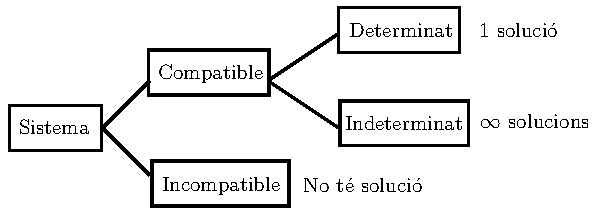
\includegraphics[width=10cm]{img-02/classificacio-sistemes.pdf}
	\end{center}

Si en aplicar el mètode de Gauss obtenim una fila de zeros $(0 0 0 | 0)$, el sistema serà compatible indeterminat (SCI). Si obtenim  una fila com  $(0 0 0 | a)$ serà incompatible (S.I.).
\end{theorybox}

 \exer \key{t2-key43} Resol pel mètode de Gauss i classifica en compatible determinat, compatible indeterminat o incompatible.
\begin{tasks}(2)
	\task  $\left\{\begin{array}{ll} x-y&=1 \\ 2x+6y-5z&=-4 \\ x+y-z&=0 \end{array}\right. $       
\task  $\left\{\begin{array}{ll} x+2y+z&=3 \\ x-2y+5z&=5 \\ 5x+22y+17z&=1 \end{array}\right. $ 
\task  $\left\{\begin{array}{ll} x+y+3z&=2 \\ 2x+3y+4z&=1 \\ -2x-y-8z&=-7 \end{array}\right. $        
\task  $\left\{\begin{array}{ll} 2x-y-z&=2 \\ 3x-2y-2z&=2 \\ -5x+3y+5z&=-1 \end{array}\right. $ 
\task  $\left\{\begin{array}{ll} x+y+z&=3 \\ -x+2y+z&=5 \\ x+4y+3z&=1 \end{array}\right. $ 
\task  $\left\{\begin{array}{ll} -2x+y+z&=1 \\ 3x+2y-z&=0 \\ -x+4y+z&=2 \end{array}\right. $ 
\end{tasks}



\exer  Desitgem vendre un cotxe, un pis i una finca per un total de 300000\euro. Si la finca val 4 vegades més que el cotxe i el pis cinc vegades més que la finca. Què val cada cosa?
\answers{Cotxe 12000 \euro{}; Finca 48000 \euro{}; Pis 240000 \euro{}}
 
	\exer  Una mare té el doble de la suma de les edats dels seus fills. L'edat del fill menor és la meitat de la seva germana. La suma de les edats dels nens i la de la mare és 45 anys. Quines edats tenen?
	\answers{$x-2y-2z=0$,\par $y-2z=0$,\par $x+y+z=45$.\par Solució: $x=30$, $y=10$, $z=5$ anys}
	 
	
	\exer  Les tres xifres d'un nombre sumen 18.  Si a aquest nombre se li resta el que resulta d'invertir l'ordre de les seves xifres, s'obté 594; la xifra de les desenes és mitja aritmètica entre les altres dues. Troba aquest nombre.
	\answers{$x+y+z=18$,\par $-99x+99z=594$,\par $y=(x+z)/2$.\par  Solució: $x=3$, $y=6$, $z=9$}
	
	
	\exer  Volem esbrinar les edats d'una família formada pels pares i els dos fills. Si sumam les seves edats de tres en tres, obtenim 100, 73, 74 i 98 anys, respectivament. Quina és l'edat de cadascun d'ells?
	\answers{$x+y+z=100$,\par $y+z+t=73$,\par $x+z+t=74$,\par $x+y+t=98$.\par Solució: $x=42$, $y=41$, $z=17$ i $t=15$ anys.}

\end{mylist}
 
\section{Inequacions}

\begin{theorybox}
	
	\video{61}{}
	
	\textbf{La solució d'una inequació es dóna en forma d'INTERVAL.}
	
	\textbf{Recorda:} Quan canviam els signes d'una inequació el sentit de la desigualtat canvia.
	
	Per exemple  $-4x + 1 > 9$, aïllam $-4x > 9-1$, i canviam els signes i el símbol $4x < -8$, que ens duu a $x<-2$, és a dir la semi-recta  $x\in (-\infty, -2)$.
\end{theorybox}

\begin{mylist}
\exer  Resol les següents inequacions i representa la solució a la recta real:
 \begin{tasks}(2)
\task $5 + 3{x} < 2{x} + 4 $
\task $3 + 4{x} \leq 8{x} + 6$ 
\task $4(3 + 2{x}) < -(6{x} + 8)$  
\task $7(2 + 3{x}) \leq 5(6{x} + 3)$
 \task $9(2 + 4{x}) + 4(5{x} - 2) > 3(2{x} + 1)$ 
 \end{tasks}
\answers{[$(-\infty,-1)$, $[9/4,+\infty)$, $(-\infty,x-10/7)$, $[-1/9,+\infty)$, $(-7/50,+\infty)$]}
 
\exer  Resol les següents inequacions i representa la solució a la recta real:
  \begin{tasks}(2)
\task $6 + 3{x} < {x}/3 + 1 $
\task $5 + 5{x}/2 \leq 9{x}/2 + 1$  
\task $(2 + 5{x})/3 > 4{x} + 1  $
\task $(1 + 5{x})/2 + 1 \geq (3{x} + 6)/4$
 \end{tasks}
  \answers{[$(-\infty,-1)$, $[2,+\infty]$, $(-\infty,-1/7)$, $[0,+\infty)$]}

 
\exer  Calcula els valors de  $x$ perquè sigui possible calcular les següents arrels:
  \begin{tasks}(2)
\task $\sqrt{2x-3} $  \task $\sqrt{-x-9} $  \task $\sqrt{2-7x} $   \task $\sqrt{-2x+7} $
 \end{tasks}
  \answers{[$[3/2,+\infty)$, $(-\infty,-9]$, $(-\infty,2/7]$, $(-\infty,7/2]$]}

\end{mylist}

\begin{example}
	\textbf{Inequacions de segon grau} 
	
	 $x^2-1 \ge 0$. Per resoldre una inequació de 2n grau, primer resoldrem l'equació canviant la desigualtat per un igual. $x^2-1 = 0$ té dues solucions $x=-1, x=1$. 
	
	\begin{center}
		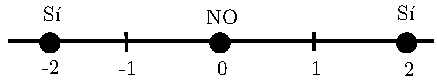
\includegraphics[width=6.5cm]{img-02/inequacion2ngrau.pdf}
	\end{center}
	La recta real ens queda divida en 3 trossos: $(-\infty,-1)$, $(-1,1)$, $(1,+\infty)$. Agafam un nombre qualsevol de cadascun dels intervals i comprovam si verifica l'inequació original $x^2-1 \ge 0$. Veim que el primer i darrer trossos són vàlids i el del mig no serveix.
	
	La solució és  $[-\infty,-1]\cup[1,+\infty]$. Hem escrit interval tancat perquè la desigualtat és major o igual.
\end{example}	
 	 
 \begin{mylist}
 		 
 	 
\exer  Resol les següents inequacions de segon grau:
  \begin{tasks}(3)
 \task $x^2-9>0$ 
 \task ${x}^{2} + 4 \ge 0$
\task $2{x}^{2} - 50 < 0$  
\task $3{x}^{2} +12 \le  0$    
\task $5{x}^{2} - 45 > 0$  
\task ${x}^{2 }+ 1 \ge  0$
 \end{tasks}
\answers[cols=1]{[$(-\infty,-3)\cup(3,+\infty)$, $\Re$, $(-5,5)$, $\emptyset$, $(-\infty,-3)\cup (3,+\infty)$, $\Re$]}

\end{mylist}



\begin{mylist}

 
\exer  Resol les següents inequacions de segon grau:
  \begin{tasks}(3)
\task $x^{2} + {x} \le 0  $ 
\task $x^{2} - 5{x} > 0 $  
\task $x^{2 } \le  8{x}$
	\task $x^{2} - 2{x} - 3 \le  0$
    \task ${-x}^{2}-2{x} + 8 \ge  0$
     \task $x^{2 }+ 9{x} + 14 > 0$
%      \task $x^{2} - 6{x} + 9 \le  0$
%\task $-x^{2 }-4{x} - 5 < 0$  
%\task $x^{2 }+ 8{x} + 16 > 0$    
 \end{tasks}

\answers[cols=1]{[$[-1,0]$, $(-\infty,0)\cup (5,+\infty)$, $[0,8]$, $[0,3]$, $(-\infty,0)\cup (3/2,+\infty)$, $(0,2)$]}
 
  \exer Per a quins valors de $x$ és possible obtenir les següents arrels?
 \begin{tasks}(4)
 	\task $\sqrt{x^{2} -1} $   \task $\sqrt{-x^{2} +4} $   \task $\sqrt{x^{2} +5x+6} $  \task $\sqrt{x^{2} -5x+6} $
 \end{tasks}
\answers[cols=1]{[$[-1,3]$, $[-4,2]$, $(-\infty,-7)\cup (-2,+\infty)$, $x=3$, $\Re$, $\Re$]}


\exer  Resol gràficament els següents sistemes d'inequacions:
  \begin{tasks}(2)
\task $\left\{\begin{array}{c} {\frac{1}{2} -\frac{x-2y+3}{3} \ge \frac{x-y+1}{2} } \\ {1-\frac{2x-4-y}{3} +\frac{2x+3y}{2} \ge 0} \end{array}\right. $  
 \task $\left\{\begin{array}{c} {x+y\ge 1} \\ {y-2x\ge 3} \\ {y\le 5} \end{array}\right. $  
 \task $\left\{\begin{array}{c} {x+y\ge 0} \\ {2x-y\ge 0} \\ {x\le 6} \end{array}\right. $  
 \task $\left\{\begin{array}{c} {(x+1)\cdot 10+x\le 6(2x+1)} \\ {4(x-10)<-6(2-x)-6x} \end{array}\right. $
 \end{tasks}
\answers{Solució gràfica:
	\par
	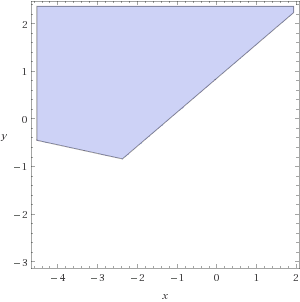
\includegraphics[width=0.3\textwidth]{img-sol/t2-55a}
	\par
	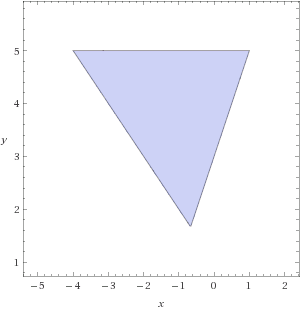
\includegraphics[width=0.3\textwidth]{img-sol/t2-55b}
	\par
	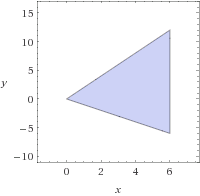
\includegraphics[width=0.3\textwidth]{img-sol/t2-55c}
	\par
	 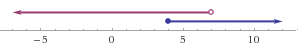
\includegraphics[width=0.4\textwidth]{img-sol/t2-55d}
}

\begin{comment}
\exer  Representa la regió factible del sistema:
\[\left\{\begin{array}{l} {x\ge 0} \\ {y\ge 0} \\ {6x+5y\le 30} \\ {x+2y\le 8} \end{array}\right. \] 
\end{comment}
\end{mylist}

\vspace{1cm}
 
\begin{autoaval}{31}

\begin{mylist}
	\exer[2] Quin és el valor numèric de l'expressió $\dfrac{3x-7}{2-3y^{2} } +5xy^{3} -\dfrac{6}{z} $ \par en $x=2,\, \, y=-1,\, \, z=-1$ ? 
\begin{comment}
  \begin{tasks}(4)
\task 17  \task 15   \task $-$3   \task $-$5
 \end{tasks}
\end{comment}
\answers{$-3$}
 
		\exer[2]  Divideix el polinomi $p(x)=x^{5} +x^{4} +x^{3} +1$ entre $q(x)=x^{2} +x+1$.
\begin{comment}
	  \begin{tasks}(2)
	 \task ha de ser de grau 2.    \task pot ser de grau 2. 
\task ha de ser de grau menor que 2.  \task cap de les opcions anteriors.
 \end{tasks}
\end{comment}
\answers{$Q=x^3$; $R=1$}

 
\exer[2]  És possible que un polinomi, amb coeficients enters, de grau quatre tingui exactament tres arrels reals, ja siguin diferents o amb alguna múltiple?  
\answers{No, si és de grau 4 pot tenir 4 arrels, que poden esser 4 reals, o be 2 arrels reals i 2 complexes o totes 4 complexes.} 
	
 
 
\exer[2]  Resol la inequació $x^{2} \leq 4$  
 \begin{comment}
   \begin{tasks}(2)
  \task {x} $\in$  ($-$2, 2)  \task {x}$\in$ [$-$2, 2]  \task {x} $\in$ ($-$$\infty$,$-$2) $\cup$ (2, +$\infty$) \task{ x}$\in$  ($-$$\infty$,$-$2] $\cup$ [2, +$\infty$)
 \end{tasks}
 \end{comment}
 \answers{$x \in [-2, 2]$}
 
\exer[2]  Resol la inequació  $\left|-x+7\right|\le 8$ 
 \begin{comment}
 
   \begin{tasks}(4)
	 \task $[-$1, 15]   
	 \task ($-$$\infty$, $-$1]  
	 \task ($-$1, 1)   
	 \task $[1$, $\infty$)
 \end{tasks}
 \end{comment}
 \answers{$[-1, 15]$}
 
\exer[2]  Resol $\sqrt{5x-9}$ 
 \begin{comment}
 
   \begin{tasks}(4)
 \task {x} $<$ 9/5  \task {x} $>$ 9/5  \task {x} $\leq$ 9/5   \task {x} $\geq$  9/5 
 \end{tasks}
 \end{comment}
 \answers{$x \geq  9/5$ }
 
\exer[2] Resol la inequació\textbf{ $\frac{2x-3}{x-2} <1$} 
 \begin{comment}
 
   \begin{tasks}(4)
\task (1, 2)  \task ($-$$\infty$, 1)   \task \textit{x} $<$ 1 $\cup$ \textit{x} $>$ 2 \task ($-$1, 2)
 \end{tasks}
\end{comment}
\answers{$x\in(1,2)$}

		\exer[2]  Justifica la veracitat o falsedat de cadascuna de les següents frases:  
\begin{tasks}
	\task  La regla de Ruffini serveix per dividir dos polinomis qualssevol.   
	%
	\task  La regla de Ruffini permet dictaminar si un nombre és arrel o no d'un polinomi.   
	%
	\task  La regla de Ruffini únicament és vàlida per a polinomis amb coeficients enters.  
	%
	\task  La regla de Ruffini és un algorisme que ens proporciona totes les arrels d'un polinomi.
\end{tasks}
\answers[cols=4]{[F, V, F, F]}

\end{mylist}
\end{autoaval}

\newpage
\resum

\begin{center}
	\setlength\LTleft{0pt}
	\setlength\LTright{0pt}
	\ftimes{10.5}{11}
	\fontsize{10.5}{11}
	\renewcommand{\arraystretch}{1}
	\begin{longtable}[h]{|>{\raggedleft\arraybackslash}p{0.19\textwidth}|p{0.77\textwidth}|}
		\hline %inserts double horizontal lines
		\rowcolor{lightgray}
		
		\textbf{Apartat} & \textbf{Resum} \\   
	  \hline
	    \begin{comment}
	    \cellcolor{lightgray}\noindent \textbf{Polinomi}  &  
		Expressió construïda a partir de la suma de monomis
		 \sample{  
			$-x^{3} +4x^{2} +8x+6$. Grau 3
		}\hline  
		 
		
			\cellcolor{lightgray}\noindent \textbf{Grau d'un polinomi}  &  
		
		El major grau dels seus monomis \\ \hline
	
		 
	    \end{comment}


	\cellcolor{lightgray}\noindent \textbf{Divisió de dos polinomis}  &  
S'obtenen altres dos polinomis, els polinomis quocient (\textit{c}(\textit{x})) i residu (\textit{r}(\textit{x})), lligats als polinomis inicials, els polinomis dividend (\textit{p}(\textit{x})) i divisor (\textit{q}(\textit{x}))
\sample{  
	$p(x)=q(x)\cdot c(x)+r(x)$
}\\ \hline

	\cellcolor{lightgray}\noindent \textbf{Regla de Ruffini}  &  
Ens pot ajudar a l'hora de factorizar un polinomi i conèixer les seves arrels \\ \hline

	\cellcolor{lightgray}\noindent \textbf{Teorema del residu}  &  

El valor numèric que adopta un polinomi $p(x)$ al particularizar-lo en $x=\alpha $ coincideix amb el residu que apareix en dividir $p(x)$ entre $x-\alpha $.\\ \hline

	\cellcolor{lightgray}\noindent \textbf{Arrel d'un polinomi}  &  
Un nombre real concret $\alpha $ és \textbf{una arrel}, o \textbf{un zero}, del polinomi $p$, si en avaluar $p$ en $x=\alpha $ obtenim el número 0, és a dir, si $p(\alpha )=0$
\sample{  
	2 és arrel de $-{3 x} + 6$. Les arrels de  $x^{2} +2x-3$ són $1$ i $-3$ 
}  \hline

	\cellcolor{lightgray}\noindent \textbf{Factorització de polinomis}  &  
Consisteix a expressar-ho com a producte d'altres polinomis de menor grau
\sample{  
	$x^{5} -3x^{3} -x^{2} +3=(x^{2} -3)\cdot (x^{3} -1)$
}  \hline

	\cellcolor{lightgray}\noindent \textbf{Fraccions algebraiques}  &  
És una fracció d'expressions polinòmiques
\sample{  
	$\dfrac{x^{2} -1}{x^{3} +x^{2} -6x} $
} \hline

	\cellcolor{lightgray}\noindent \textbf{Equacions de 2n grau}  &  
Igualtats algebraiques amb una sola incògnita i elevada al quadrat.
\sample{  
	$-x^{2} +4x+5$\newline La solució del qual és: 
	$x_1=-1$ i $x_2=5$.
} \hline

	\cellcolor{lightgray}\noindent \textbf{Equacions biquadrades}  &  
És una equació del tipus $ax^4 + bx^2+c=0$. Si es fa el canvi $t=x^2$, l'equació anterior es tranforma en una de segon grau $a t^2 + b t + c=0$. Les solucions es troben fent $x=\pm \sqrt{t}$
\\ \hline


\cellcolor{lightgray}\noindent \textbf{Sistemes d'equacions lineals. Gauss }  &  
Resolució pel mètode de Gauss.
\sample{
	\[
		\left\{
		\begin{array}{lcl}
		x+4y+3z &=&-1 \\
		2x-3y-2z &=&1 \\
		x+2y+4z=2
		\end{array}
		\right.
	\]  
} \hline
	
	\cellcolor{lightgray}\noindent \textbf{Inequacions de 1r grau }  &  
Desigualtats algebraiques amb una sola incògnita  de grau 1. La solució expressa en forma d'una semi-recta.
\sample{  
	$\frac{x-3}{3} -\frac{(x-7)}{6} >\frac{4-x}{2}$, \quad té solució $x>\frac{11}{4}$ o $(\frac{11}{4}, +\infty)$.
} \hline

	\cellcolor{lightgray}\noindent \textbf{Inequacions de 2n grau }  &  
Desigualtats algebraiques amb una sola incògnita, elevades al quadrat. La solució expressa en forma d'interval.
\sample{  
	$x^2-6x+5>0$ la seva solució és l'interval (1, 5). 
}  \hline 
	\end{longtable}
\end{center}

\mychapter{Trigonometria}{Trigonometria}{

\includegraphics[width=4cm]{img-03/chap3.png}
}
{chap:trig}
 

\section{Raons trigonomètriques}
	\subsection{Raons trigonomètriques d'angle agut}

\begin{theorybox}
	
	Definim les raons trigonomètriques d'un angle agut d'un \textbf{triangle rectangle} com
	
	\begin{center}
		\textbf{sinus}: $\sin \alf = \dfrac{C.O.}{H}$, \textbf{cosinus}: $\cos \alf = \dfrac{C.C.}{H}$ i \textbf{tangent}: $\tg \alf = \dfrac{C.O.}{C.C.}$
	\end{center}
	
	essent $H$ la hipotenusa, $C.O.$ el catet oposat a l'angle i $C.C.$ el catet contigu. 
	
	També definim les raons recíproques com 
	
	\begin{center}
		\textbf{cosecant}:	$\cosec \alf = \dfrac{1}{\sin \alf}$, \textbf{secant}: $\sec \alf = \dfrac{1}{\cos \alf}$ i \textbf{cotangent}: $\cotg \alf = \dfrac{1}{\tg \alf}$.
	\end{center}
	
	
	\begin{minipage}{0.65\textwidth}
		\vspace{-0.75cm}	
		\video{122}{Raons d'un angle agut}
		
		\vspace{0.4cm}
		Representació de les raons trigonomètriques per un angle agut. Les raons no depenen de 
		la mida del triangle; només de l'angle.
	\end{minipage}
	\begin{minipage}{0.35\textwidth}
		
		\begin{center}
			\includegraphics*[width=0.8\textwidth]{img-03/chap-trig-grafraons.png}
		\end{center}
	\end{minipage}
\end{theorybox}

\begin{mylist}
	\exer
	A partir d'un triangle rectangle i aplicant el teorema de \emph{Pitàgores}, demostra la primera relació fonamental de la trigonometria $\sin^2 \alpha + \cos^2 \alpha = 1$.
	
	\answers{Si el triangle rectangle té hipotenusa $a$ i catets $b$ i $c$. Es compleix per trigonometria que $b=a\cos \alpha$ i $c=a\sin \alpha$. Si aplicam el teorema de Pitàgores a aquest triangle $a^2 = b^2 + c^2$, trobam que $a^2 = (a\cos \alpha)^2+ (a\sin \alpha)^2$. Finalment, simplificam dividint entre $a^2$  trobam $\sin^2 \alpha + \cos^2 \alpha = 1$.}
 	
	\exer
	Utilitzant les definicions de les raons trigonomètriques, demostra la
	segona relació fonamental $\tg \alpha = \dfrac{\sin \alpha}{\cos \alpha}$.
	\answers{$\dfrac{\sin \alpha}{\cos \alpha}=\dfrac{\frac{CO}{H}}{\frac{CC}{H}}=\dfrac{CO}{CC}=\tg \alpha$}
	
	\exer
	Utilitzant la definició de les raons, demostra les identitats:
	\begin{tasks}(2)
		\task $1+\tg^2 \alf = \sec^2 \alf$
		\task $1+\cotg^2 \alf = \cosec^2 \alf$
	\end{tasks}
	
	Comprova les anteriors relacions a partir dels angles de
	30${}^\circ$ i 60 ${}^\circ$.
	\answers{a) Parteix de $\sin^2 \alpha + \cos^2 \alpha = 1$ i divideix tot entre $\cos^2 \alpha$.\par b) Parteix de $\sin^2 \alpha + \cos^2 \alpha = 1$ i divideix tot entre $\sin^2 \alpha$}
	
	\exer
	Explica, a partir del vist en aquest apartat, perquè el sinus i el
	cosinus de 45${}^\circ$ són iguals, i perquè la tangent val
	la unitat.
	\answers{A 45 graus, resulta que CC=CO i per això $\sin 45 = \cos 45$.\par Com que la $\tg 45 = \dfrac{CO}{CC}=1$.}
\end{mylist}

\begin{theorybox}[Raons d'angles notables aguts]
	\videonw{124}{Trigonometria: Demostració de les raons dels angles notables 0, 30, 45, 60 i 90 graus}
	
	\begin{center}
		\renewcommand*{\arraystretch}{1.3}
		\begin{longtable}{|P{0.15\textwidth}|P{0.15\textwidth}|P{0.15\textwidth}|P{0.15\textwidth}|P{0.15\textwidth}|}
			\rowcolor{lightgray} Angle $\alpha$ (${}^\circ$) & Angle $\alpha$ (rad) & $\sin \alpha$ & $\cos \alpha$ & $\tg \alpha$ \\ \hline
			0 & 0 & 0 & 1 & 0 \\ \hline
			30 & $\frac{\pi}{6}$ & $\frac{1}{2}$  & $\frac{\sqrt{3}}{2}$  & $\frac{\sqrt{3}}{3}$ \\ \hline
			45 & $\frac{\pi}{4}$ & $\frac{\sqrt{2}}{2}$ & $\frac{\sqrt{2}}{2}$  & 1 \\ \hline
			60 & $\frac{\pi}{3}$ & $\frac{\sqrt{3}}{2}$  & $\frac{1}{2}$  &  $\sqrt{3}$ \\ \hline
			90 & $\frac{\pi}{2}$ & 1 & 0 & $--$ \\ \hline
		\end{longtable}
		
	\end{center}
	
\end{theorybox}

\subsection{Angles i raons trigonomètriques inverses}


\begin{theorybox} 
	\video{123}{}
	
	\textbf{Radiant}
	
	Un angle de 1 rad $\approx 57,3^\circ$. A la pràctica utilitzam el factor de conversió 
	\begin{equation*}
	2\pi\,\, \mathrm{rad} = 360^\circ.
	\end{equation*} 
\end{theorybox}

\begin{mylist}
	\exer Expressa en radiants els angles següents: 60${}^\circ$, 120${}^\circ$, 225${}^\circ$, 330${}^\circ$.
	\answers{$\frac{\pi}{3}$, $\frac{2}{3}\pi$, $\frac{5}{4}\pi$, $\frac{11}{6}\pi$}
	\begin{example}[*]
		\begin{equation*}
		60^\circ \cdot \frac{2 \pi \,\,\mathrm{rad}}{360^\circ} = \frac{60}{180}\pi = \frac{\pi}{3} \,\,\mathrm{rad}
		\end{equation*}
	\end{example}
	
	\exer 
	Expressa en graus sexagesimals: $\dfrac{\pi}{4}$, $\dfrac{2\pi}{3}$, $\dfrac{3\pi}{2}$ i $\dfrac{10\pi}{6}$ radiants.
	\answers{$45^\circ$, $120^\circ$, $270^\circ$, $300^\circ$}
	
	\exer 
	Quant sumen (en radiants) els angles d'un triangle? Quant mesura un
	angle recte en radiants?
	\answers{Els angles d'un triangle sumen $\pi$ radiants. Un angle recte són $\pi/2$ radiants.}
	
	\exer
	Per veure la utilitat dels radiants, suposem un mòbil que es mou en
	una circumferència de dos metres de radi amb una velocitat de 4 m/s.
	Calcula la seva velocitat en rad/s i en graus per segon. Quantes
	voltes dóna per minut?
	\answers{$\omega=v/R=2$ rad/s. En un minut \linebreak $2$ rad/s $\cdot 60 $s$ = 120 $ rad = 19.1 voltes}
	
	\exer
	Un mòbil ha recorregut un angle de 3 rad en una circumferència de radi 2 m. Quant
	espai ha recorregut? I si la circumferència tingués radi 0'5 m? \emph{Recorda}:  
	L'arc de circumferència $s$ és $s=\alpha\cdot R$ si l'angle $\alpha$ ve en radiants.
	\answers{6 m i 1.5 m}
	
\end{mylist}


\subsection{Raons trigonomètriques d'angles qualssevol}
\begin{theorybox}
	\video{125}{Raons trigonomètriques d'angles qualssevol}
	
	Signe de les raons trigonomètriques segons el quadrant:
	\begin{center}
		\includegraphics*[width=0.4\textwidth]{img-03/chap-trig-signesraons.png}
	\end{center}
\end{theorybox}

\begin{blueshaded}
	La calculadora té dos modes per manejar angles, \textbf{DEG} graus i \textbf{RAD} radiants. Per aquesta activitat assegura't que el tens en mode \textbf{DEG}.
	
	\begin{minipage}{0.6\textwidth}
		Les funcions trigonomètriques inverses de la calculadora donen només un dels possibles possibles de l'angle. Aquest angle es troba entre:
	\end{minipage}
	\begin{minipage}{0.4\textwidth}
		\begin{center}
			\begin{tabular}{c|c}
				$\arcsin x$ & $-90^\circ$ a $90^\circ$ \\ \hline
				$\arccos x$ & $0^\circ$ a $180^\circ$ \\ \hline
				$\arctg x$ & $-90^\circ$ a $90^\circ$ \\	
			\end{tabular}
		\end{center}
	\end{minipage}
	
	L'altre angle l'has d'obtenir raonant amb l'ajuda de la circumferència goniomètrica.
	
	\textbf{Quins angles tenen per sinus 0,5?}
	
	Una resposta l'obtenim de la calculadora \tecla{SHIFT} \tecla{sin} 0,5 \tecla{=} \pantalla{30}.
	
	L'altre angle es troba al segon quadrant, i l'obtenim fent $180^\circ-30^\circ=150^\circ$
	
	\textbf{Quins angles tenen per tangent -2?}
	
	Una resposta l'obtenim de la calculadora \tecla{SHIFT} \tecla{tan} -2 \tecla{=} \pantalla{-63.4349...}. Aquest angle es troba al quart quadrant i en
	realitat és l'angle $360-63,4349=296.5651$.
	
	L'altre angle s'ha de trobar al segon quadrant, on també la tangent és negativa. El trobam fent $180^\circ-63,3349^\circ=116,5651^\circ$
\end{blueshaded}
\begin{mylist}	
	\exer
	Copia en el teu quadern, i situa en el quadrant que correspongui i
	expressa en funció d'un angle agut les raons trigonomètriques dels
	següents angles:
	\begin{tabular}{|p{0.10\textwidth}|p{0.11\textwidth}|p{0.11\textwidth}|p{0.11\textwidth}|p{0.11\textwidth}|p{0.11\textwidth}|p{0.11\textwidth}|}
		\toprule
		Angle & Sinus & Cosinus & Tangent & Secant & Cosecant & Cotangent \\
		\midrule
		120$^\circ$ & & & & & & \\ \hline
		135$^\circ$ & & & & & & \\ \hline
		210$^\circ$ & & & & & & \\ \hline
		315$^\circ$ & & & & & & \\ \hline
		390$^\circ$ & & & & & & \\ \hline
		3000$^\circ$ & & & & & & \\ \hline
		$-150^\circ$ & & & & & & \\  
		\bottomrule
	\end{tabular}
\answers{ $\bullet$ \textbf{120 = 180--60} \par\par
	$\sin 120=\sin 60$\par$\cos 120=-\cos 60$\par$\tg 120=-\tg 60$\par\par
	$\bullet$ \textbf{135 = 180--45} \par\par
	$\sin 135=\sin 45$\par$\cos 135=-\cos 45$\par$\tg 135=-\tg 45$\par\par
	$\bullet$ \textbf{210 = 180+30} \par\par
	$\sin 210=-\sin 30$\par$\cos 210=-\cos 30$\par$\tg 210=\tg 30$\par\par
	$\bullet$ \textbf{315= 360--45} \par\par
	$\sin 315=-\sin 45$\par$\cos 315=\cos 45$\par$\tg 315=-\tg 45$\par\par
	$\bullet$ \textbf{390 = 30} \par\par
	$\sin 390=\sin 30$\par$\cos 390=\cos 30$\par$\tg 390=\tg 30$\par\par
	$\bullet$ \textbf{3000 = 120} \par\par
	$\sin 3000=\sin 120$\par$\cos 3000=\cos 120$\par$\tg 3000=\tg 120$\par\par
	$\bullet$ \textbf{--150 = 210} \par\par
	$\sin -150=\sin 210$\par$\cos -150=\cos 210$\par$\tg -150=\tg 210$\par\par
}
	
	\exer
	Utilitza la calculadora i l'après en aquest apartat per trobar tots
	els angles positius menors que 360${}^\circ$ el sinus dels quals
	és de 0'6.
	\answers{Una solució $\arcsin 0,6=36.87^\circ$ l'altre és $180-36.87 =143.13^\circ$}
	
	\exer
	Troba tots el angle compresos entre 0 i $360^\circ$ la tangent dels quals val 4.
	\answers{Una solució $\arctg 4=75.96^\circ$ l'altre és $180+75.96 =255.96^\circ$}
	
	\exer
	Troba tots el angle compresos entre 0 i $360^\circ$ el cosinus dels quals val 0'75.
	\answers{Una solució $\arccos 0.75=41.41^\circ$ l'altre és $360-41.41 =318.59^\circ$}
	
\end{mylist}	



\section{Resolució de triangles}

\subsection{Triangles rectangles}

\begin{theorybox}
	\begin{wrapfigure}{r}{4cm}
		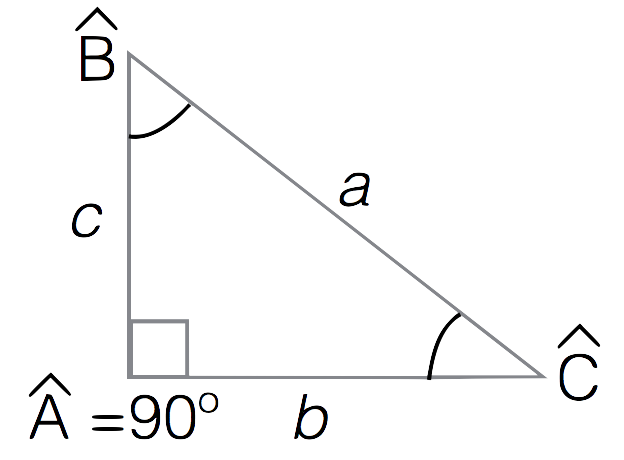
\includegraphics[width=4cm]{img-03/triangle-rectangle1}
	\end{wrapfigure}
	En un triangle rectangle, sempre utilitzarem el següent conveni per anomenar els costats i angles. L'angle recte és $\hat A=90^\circ$.
	
	Podrem utilitzar les següents relacions
	\begin{eqnarray*}
		\hat B=90-C, & a^2 = b^2 + c^2
	\end{eqnarray*}
	\begin{eqnarray*}
		b=a \cos \hat C, & c=a \sin \hat C, & \tg \hat C= \dfrac{c}{b}
	\end{eqnarray*}	
\end{theorybox}

\begin{resolt}[E]{Resol el triangle rectangle del qual sabem que \linebreak $\hat B=50^\circ$ i el catet $c=15$ cm.}
	
	\begin{wrapfigure}{r}{3.75cm}
		\vspace{-0.3cm}
		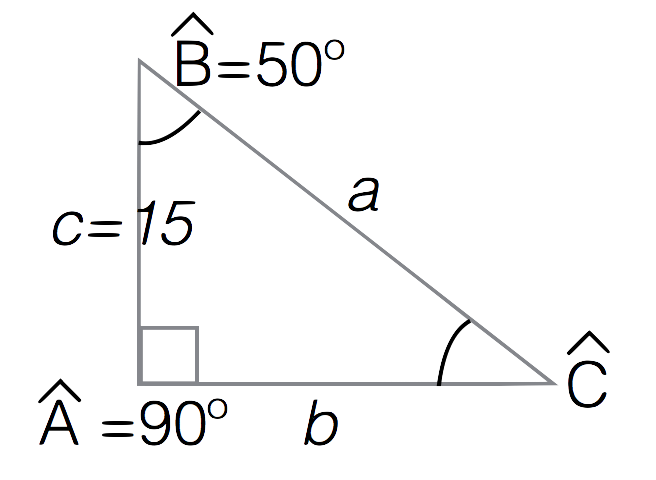
\includegraphics[width=3.5cm]{img-03/triangle-rectangle2}
	\end{wrapfigure}
	L'angle $\hat C$ s'obté de $\hat C=90-50 = 40^\circ$.
	
	Tot seguit, utilitzam la raó trigonomètrica \vspace{0.25cm}
	
	$\tg 40 = \dfrac{15}{b}$  $\rightarrow$ $b=\dfrac{15}{\tg 40}=17,87$.
	
	Del teorema de Pitàgores, $a^2 = b^2 +c^2$, \vspace{0.25cm}
	
	$a=\sqrt{15^2+17,87^2}=23,34$
	
\end{resolt}


\begin{mylist}
	
	\exer[1] Resol el triangle ABC (calcula els elements que falten), essent A l'angle recte
	\begin{tasks}(2)
		\task a=32 cm, B=57$^\circ$
		\task a=72 cm, C=23$^\circ$
		\task c=250 m, b=308 m
		\task c=35 m, C=32$^\circ$
	\end{tasks}
	\answers[cols=1]{[$\hat C=33$; $b=26,8$; $c=17,4$,  $\hat B=67$; $b=66,3$; $c=28,1$,  $\hat C=39$; $\hat B=51$; $a=396,7$,  $\hat B=58$; $b=56,01$; $a=66,05$]}
	
	\exer[1] Per arribar a una alçada de 3 m, recolçam una escala formant un angle de 60$^\circ$ amb el terra. Troba la longitud de l'escala i la distància des de la base fins a la paret.
	\answers{$a=3,46$; $b=1,73$}
	
	\exer[1] L'estatura d'una persona és 1,78 m i projecta al terra una ombra de 85 cm. Quin angle formen els rajos del sol amb l'horitzontal del terra?
	\answers{$\alpha=25,5^\circ$}
	
	\exer[1]
	Calcula els costats i els angles del triangle \emph{ABC}, rectangle en
	A, del que coneixem el catet \emph{AC} = 15cm i l'altura relativa a
	la hipotenusa \emph{AD} = 12cm.
	\answers{ $a=25$; $c=20$; $\hat B=36,87^\circ$; $\hat C=53,13^\circ$}
	
 
	\exer
	En un tram de carretera la inclinació és del 5 \% (puja 5 m en 100 m).
	Calcular l'angle que forma amb l'horitzontal la carretera. Sabem que
	hem pujat 100 m, quant hem caminat per la carretera?
	\answers{$\tg \alpha = 5/100$, $\alpha = 2.86^\circ$. $s=\frac{h}{\tg \alpha} = \frac{ 100}{\tg 2.86}=2000$ m. Hem caminat 2 km.}
	
	
	\exer \spicy[1] Una estàtua de 2,5 m d'altura està col·locada sobre una peanya. Des d'un punt del terra es veu la peanya amb un angle de 15$^\circ$ i l'estàtua, sobre un angle de 40$^\circ$. Quina és l'altura de la peanya?
	\answers{$x=\dfrac{2.5}{\tg 40 - \tg 15}=4.377$ m;  $y=x \tg 15 = 1.173$ m}
	
\end{mylist}

\subsection{Teorema del sinus}

\begin{theorybox}
	\video{127}{Trigonometria: Teorema del sinus}
	
	Sempre utilitzarem el següent conveni per anomenar els costats i angles.
	
	\begin{wrapfigure}{R}{4.5cm}
		\centering
		\vspace{-1.5cm}
		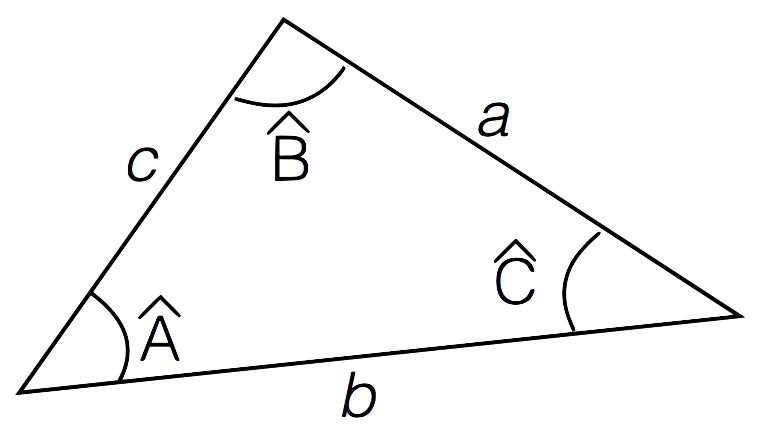
\includegraphics[width=4.5cm]{img-03/triangle-qualsevol1}
	\end{wrapfigure}
	
	D'una banda sabem que els angles compleixen $\hat A+\hat B+\hat C=180^\circ$. El teorema del sinus diu que 
	\begin{eqnarray*}
		\frac{a}{\sin \hat A}=\frac{b}{\sin \hat B}=\frac{c}{\sin \hat C}=2R
	\end{eqnarray*}
	on $R$ és el radi de la circumferència circumscrita en el triangle.
	
	De vegades, a l'aplicar el teorema del sinus, poden aparèixer dues solucions. 
	\vspace{0.7cm}
	
\end{theorybox}

\begin{resolt}[E]{En un triangle coneixem dos dels seus angles i un costat: A=55${}^\circ$, B=98${}^\circ$, a=7,5 cm. Resol el triangle.
		\begin{center}
			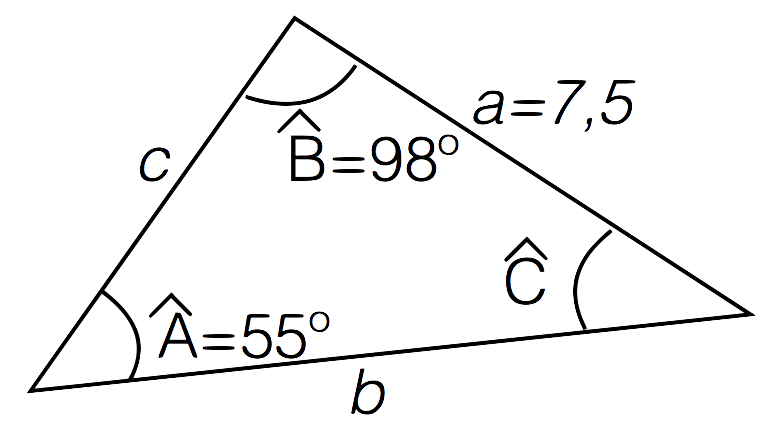
\includegraphics[width=4cm]{img-03/triangle-qualsevol2}
		\end{center}
}
	
	
	
	L'angle $\hat C=180 -(55+98)=27^\circ$
	
	Amb el teorema del sinus trobam els costats que falten
	\begin{eqnarray*}
		\frac{b}{\sin 98}= \frac{7,5}{\sin 55} \,\, \rightarrow \,\,  b=\frac{7,5 \sin 98}{\sin 55}=9,1 \,\mathrm{cm}\\
		\frac{c}{\sin 27}= \frac{7,5}{\sin 55} \,\, \rightarrow \,\,  c=\frac{7,5 \sin 27}{\sin 55}=4,2 \,\mathrm{cm}
	\end{eqnarray*}
	
	
\end{resolt}
\vspace{0.5cm}


\begin{mylist} 
	\exer
	Un triangle té dos angles que valen 40 i 60 graus respectivament. El
	costat entre ells és de 8 cm. Calcula tots els seus angles i costats.
	\answers{Costats:
		a = 5.22163 m
		b = 7.03508 m
		c = 8 m \par
		Angles:
		A = 40 
		B = 60 
		C = 80}
	
	\exer
	En un triangle \emph{ABC}, els costats \emph{AB} \emph{i AC} mesuren 3
	i 2 cm respectivament. L'angle corresponent al vèrtex \emph{B} mesura
	30 graus. Resol el triangle.
	\begin{tasks}
		\task Utilitza el teorema del sinus per calcular l'altre angle. Hi ha dues
		solucions perquè hi ha dos angles amb el mateix sinus. Calcula els dos.
		%
		\task Les dues solucions es deuen al fet que existeixen dos triangles, series
		capaç de dibuixar-los?
	\end{tasks}
	\answers{Té dues solucions:\par
	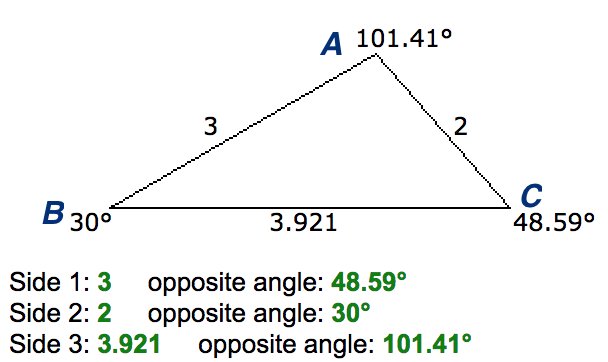
\includegraphics[width=0.4\textwidth]{img-sol/t3-21a}
	\par
	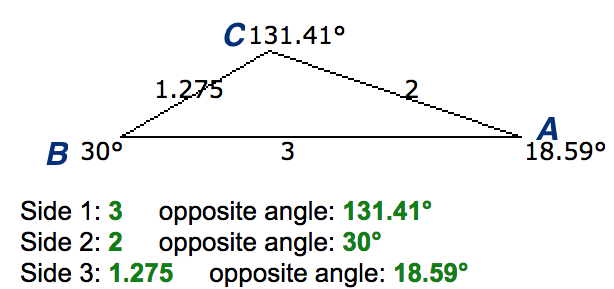
\includegraphics[width=0.4\textwidth]{img-sol/t3-21b}}
	
	
	\exer
	En un triangle coneixem dos dels seus angles i un costat: \emph{A=}55${}^\circ$, \emph{B}=98${}^\circ$, \emph{a=}7'5 cm. Resol-ho.
	\answers{Solució única:\par
		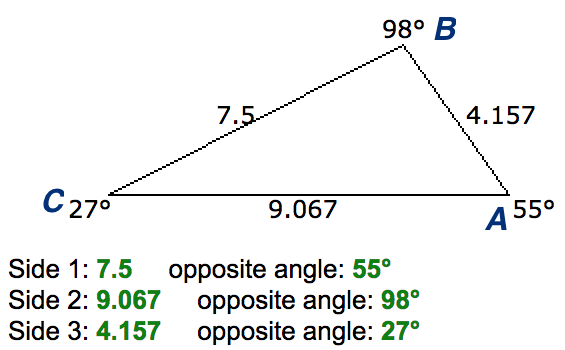
\includegraphics[width=0.4\textwidth]{img-sol/t3-22}}
		
	\exer El radi de la circumferència circumscrita al triangle ABC mesura $2\sqrt{2}$ i dos dels seus angles fan 60${}^\circ$ i 45${}^\circ$. Resol el triangle i troba'n l'àrea.
	

\answers{En primer lloc trobam dos costats a partir del radi: $a=4\sqrt{2}\sin 60=2\sqrt{6}$ i $b=4\sqrt{2} \sin 45 = 4$.\par 	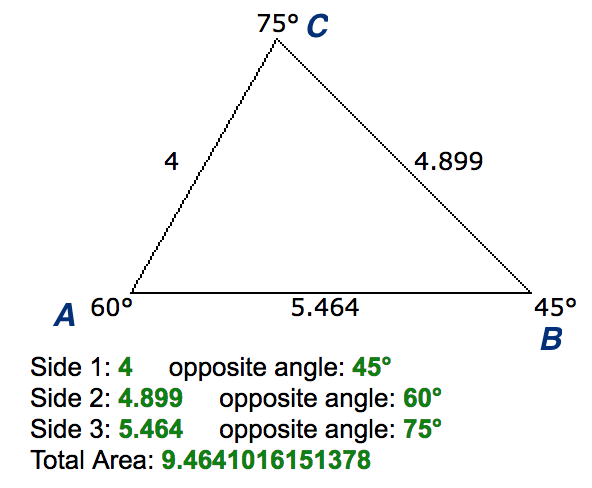
\includegraphics[width=0.4\textwidth]{img-sol/t3-23}}
	
	
	\exer
	Un globus està en la vertical entre dos observadors separats per 40 m.
	El primer ho veu amb un angle de 30 graus i el segon amb un angle de
	50 graus, a quina altura està el globus?
	
	\answers{En primer lloc resolem el triangle:\par 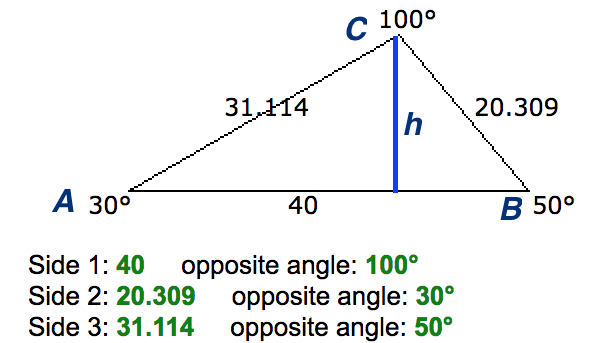
\includegraphics[width=0.4\textwidth]{img-sol/t3-24}\par
	Després calculam l'altura del triangle $h=31.1\sin 30=20.31\sin 50=15.6$ m}
	
	
	
	\exer
	Una antena de radi està subjecta al terra amb dos cables, que formen
	amb l'antena angles de 36${}^\circ$ i 48${}^\circ$. Els punts de subjecció dels cables	estan alineats amb el peu de l'antena i disten entre sí 98 metres.
	Calcula l'altura de l'antena.
	
	\answers{En primer lloc resolem el triangle:\par 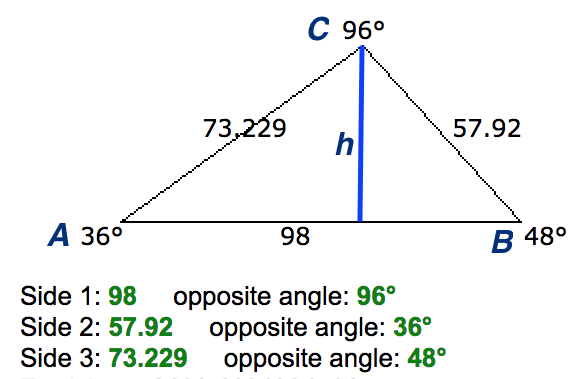
\includegraphics[width=0.4\textwidth]{img-sol/t3-25}\par
		Després calculam l'altura del triangle $h=73.23\sin 36=57.92\sin 48=43.04$ m}
	
	\exer
	Des d'un cert punt del terra es veu un arbre sota un angle de 42${}^\circ$. Baix
	quin angle es veu col·locant-se al doble de distància?
	\answers{La tangent de l'angle es redueix a la meitat: $\tg \alpha' = \frac{1}{2}\tg \alpha=\frac{1}{2}\tg 42=0.4502$, el nou angle és $\alpha'=\arctg 0.4502=24.24^\circ$. Evidentment no és la meitat de 42${}^\circ$.}
	
	\exer
	Dos amics estan en una platja a 150 m de distància i en el mateix
	plà vertical que un estel que es troba volant entre tots dos. En un
	moment donat, un el veu amb un angle d'elevació de 50${}^\circ$ i l'altre amb
	un angle de 38$^\circ$. Quina distància hi ha des de cadascun d'ells a
	l'estel? A quina altura vola l'estel?
	\answers{En primer lloc resolem el triangle:\par 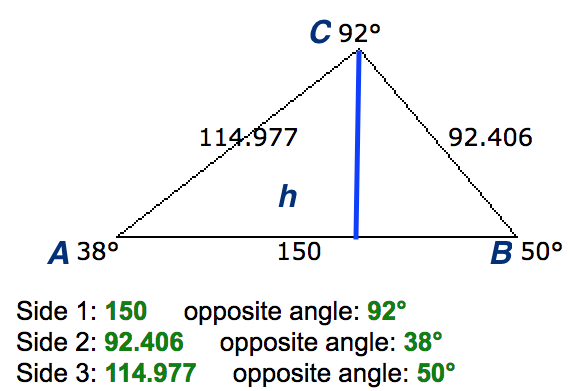
\includegraphics[width=0.4\textwidth]{img-sol/t3-27}\par
		Les distàncies de cadascú a l'estel són 115 m i 92.4 m. Després l'altura del triangle $h=114.98\sin 38=92.406\sin 50=70.79$ m}
	
	\exer
	Un globus aerostàtic es troba subjecte al terra mitjançant dos cables
	d'acer, en dos punts que disten 70 metres. El cable més curt mesura 90
	metres i l'angle que forma l'altre cable amb el terra és de 42${}^\circ$.
	Calcula:
	
	\begin{tasks}	 
		\task
		La mesura de l'altre cable.
		\task
		La distància del globus al terra.
	\end{tasks}

\answers{L'angle del triangle és $180-42=138$. En primer lloc resolem el triangle:\par 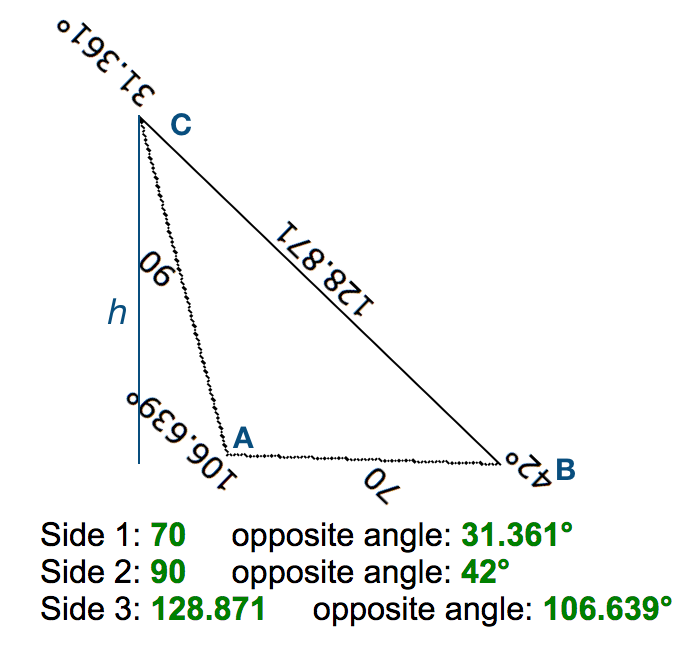
\includegraphics[width=0.4\textwidth]{img-sol/t3-28}\par
	L'altre cable mesura 128.87 m. La distància del globus al terra $h=128.87\sin 42=86.23$ m}
	
\end{mylist}

\subsection{Teorema del cosinus}

\begin{theorybox}
	\video{129}{Trigonometria: Teorema del cosinus}
	
	El teorema del cosinus s'aplica quan no tenim cap angle o quan tenim dos costats i l'angle que formen.
	El teorema es pot formular en tres versions diferents:
	\begin{eqnarray*}
		a^2 = b^2 + c^2 - 2  b \cdot c \cdot \cos\hat A \\
		b^2 = a^2 + c^2 - 2 a \cdot c\cdot \cos \hat B \\
		c^2 = a^2 + b^2 - 2 a \cdot b\cdot \cos \hat C 
	\end{eqnarray*}
	
	
\end{theorybox}


\begin{resolt}[E]{ En un triangle coneixem dos costats i l'angle comprès entre ells $\hat A$=35${}^\circ$, $b$=20 cm, $c$=14 cm. Resol-ho.}
	Aplicam el teorema del cosinus per trobar el costat oposat a l'angle A que ens donen. $a^2 = 20^2 + 14^2 - 2 \cdot 20 \cdot 14 \cos 35^\circ$.
	D'aquí aïllam el costat $a=11,72$ cm.
	
	Tornam a aplicar el teorema del cosinus ara pel costat $b$.
	
	$20^2 = 11,72^2 + 14^2 - 2 \cdot 11,72 \cdot 14 \cos \hat B$. D'aquesta fórmula cal aïllar el $\cos \hat B$,
	
	\begin{equation*}
	\cos \hat B = \dfrac{20^2 - 11,72^2 - 14^2}{-2 \cdot 11,72 \cdot 14}=-0,203
	\end{equation*}
	
	L'angle $\hat B=\arccos -0,203 = 101,7^\circ$, i finalment l'angle 
	
	 $\hat C=180-35-101,7=43,28^\circ$.
\end{resolt}

\begin{resolt}{Si els braços d'un compàs fan 12 cm de llarg i formen un angle de 60${}^\circ$, calcula el radi de la circumferència que podem traçar amb el compàs.}
	Aplicam el teorema el cosinus
	\begin{equation*}
	a^2 = 12^2 + 12^2 - 2 \cdot 12 \cdot 12 \cos 60^\circ
	\end{equation*}
	D'aquí s'obté que el costat oposat a l'angle de 60${}^\circ$ és de $a=12$, que correspon al radi
	de la circumferència que podem dibuixar. Es tracta d'un triangle isòsceles.
\end{resolt}

\begin{mylist}
	
	
	\exer
	Troba els angles d'un triangle del que es coneixen els tres costats:
	\emph{a=} 37 cm, \emph{b} = 42 cm, \emph{c} = 68 cm.
	
	\answers{$\hat A=28.52^\circ$, $\hat B=32.82^\circ$, $\hat C=118.66^\circ$}
	
	\exer
	Dibuixa un triangle amb b=5, c = 8 i l'angle entre ells de 30${}^\circ$ (usa
	una regla i un transportador). Calcula l'altre costat amb el teorema
	del cosinus i comprova que coincideix amb el resultat mesurat. No et
	sortirà exactament per l'arrodoniment i l'error de mesurament però
	hauria de ser molt similar.
	\answers{Triangle:\par 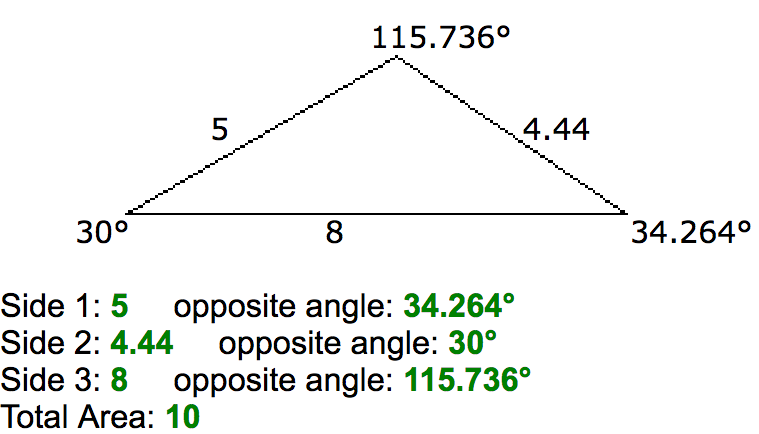
\includegraphics[width=0.4\textwidth]{img-sol/t3-30}}
	
	\exer
	Un triangle té de costats 3, 5 i 7. Calcula els seus angles.
		
	\answers{$\hat A=21.79^\circ$, $\hat B=38.21^\circ$, $\hat C=120^\circ$}
	
	
	\exer
	En un triangle \emph{ABC}, els costats \emph{AB} i\emph{AC} mesuren 3
	i 2 cm respectivament. L'angle corresponent al vèrtex \emph{B} mesura
	30 graus.
	
	a) Utilitza el teorema del cosinus per calcular l'altre costat.
	Obtindràs dues solucions.
	
	b) Les dues solucions es deuen al fet que hi ha dos triangles series
	capaç de dibuixar-los?
	
	\answers{Solució 1:\par
	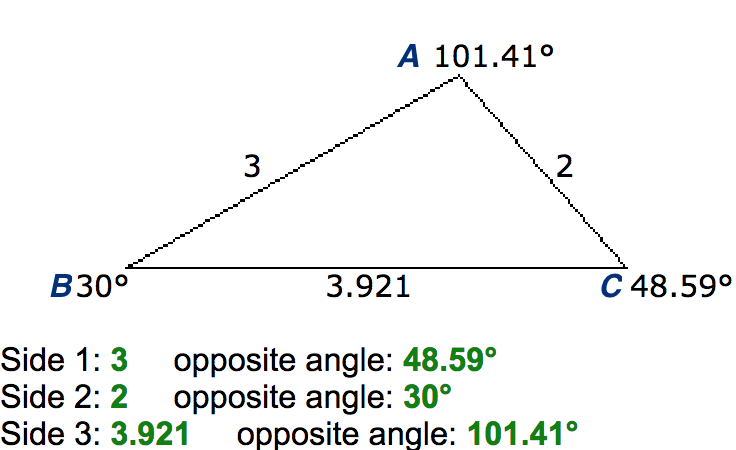
\includegraphics[width=0.4\textwidth]{img-sol/t3-32a}
	\par Solució 2:\par
	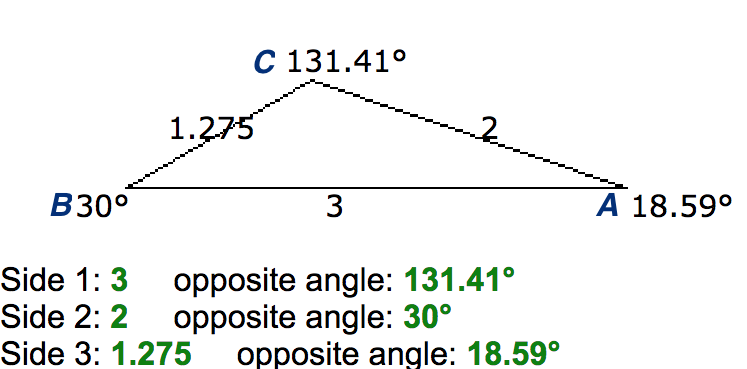
\includegraphics[width=0.4\textwidth]{img-sol/t3-32b}
}
	
	\exer
	Calcula  l'àrea d'un heptàgon regular inscrit en una circumferència de
	35 cm de perímetre.
	\answers{El radi de la circumferència $R=L/2\pi=5.57$ cm. El costat de l'heptàgon és $c=4.83$ cm  i l'apotema $a_p=5.02$  i l'àrea $A=84.9$ cm$^2$.\par 	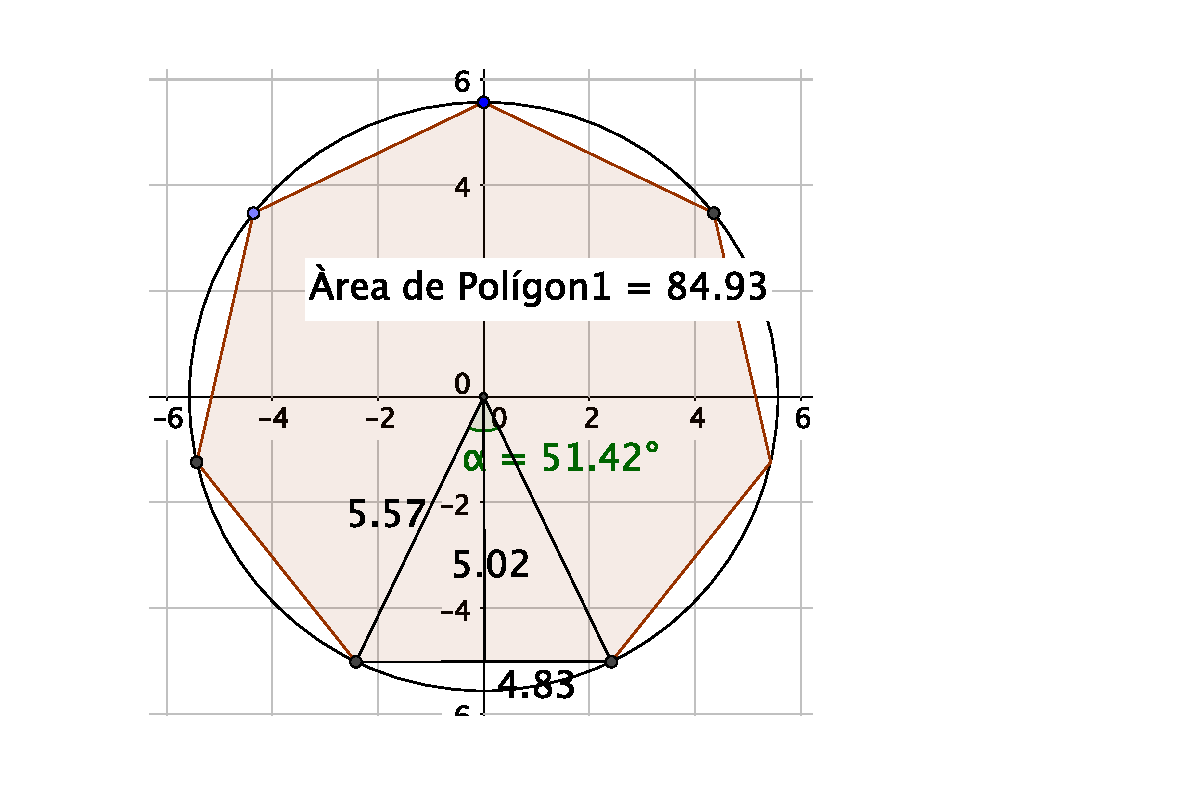
\includegraphics[width=0.3\textwidth]{img-sol/t3-33}}  
	
	\exer
	Dos vaixells parteixen d'un port amb rumbs diferents que formen un
	angle de 127${}^\circ$. El primer surt a les 10 h del matí amb una velocitat de
	17 nusos, i el segon surt a les 11 h 30 min, amb una velocitat de 26
	nusos. Si l'abast dels seus equips de radi és de 150 km. Podran
	posar-se en contacte a les 3 de la tarda? (nus=milla/hora; milla=1850
	m).
		\answers{Les distàncies en km recorregudes per cada vaixell són: $15\cdot 5 \, h \cdot 1.85=157.25$ km i  $26\cdot 3.5 \,h \cdot 1.85=168.35$ km. A les 15:00 es troben separats per 291.43 km que és superior a l'abast de le radi.\par 	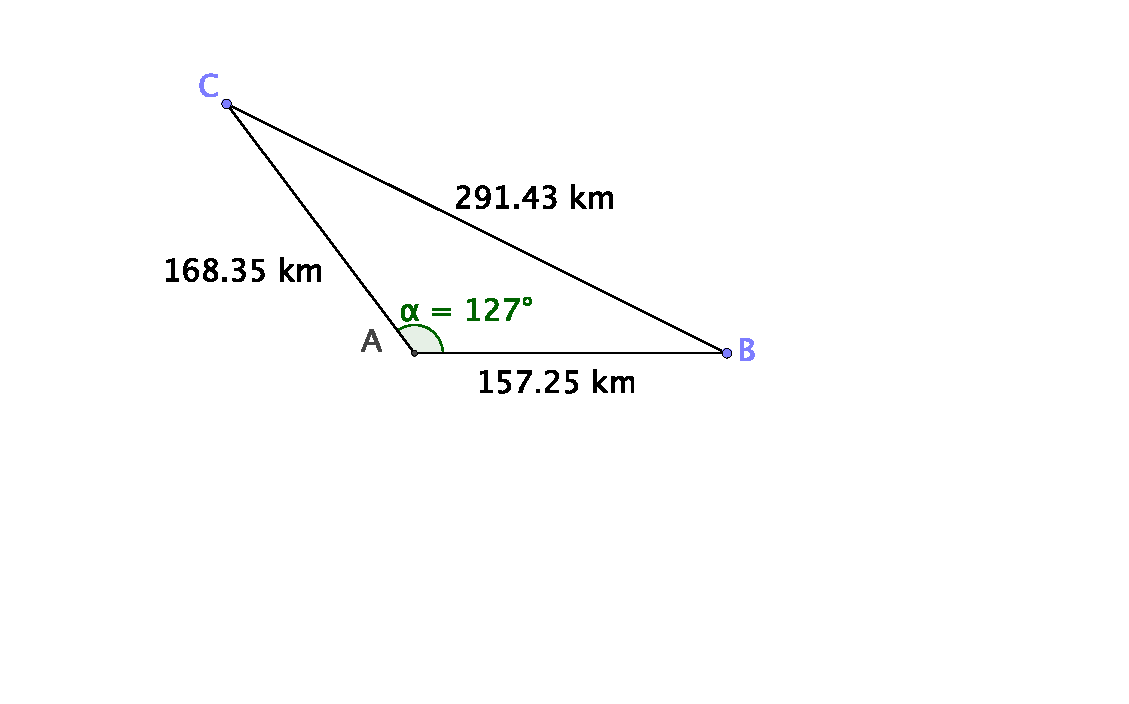
\includegraphics[width=0.4\textwidth]{img-sol/t3-34}}  
	
\end{mylist}

\subsection{Resolució de triangles en general}
\begin{mylist}
	
	
   	\vspace{-3cm}
\exer \begin{minipage}[t]{0.4\textwidth}
	Resol els següents triangles:  \vspace{0.2cm}
	\begin{tasks}
		\task B=30${}^\circ$, \emph{a}=5 cm, \emph{b} = 6 cm \vspace{0.2cm}
		\task A=45${}^\circ$, C=60${}^\circ$, \emph{b} = 20 m \vspace{0.2cm}
		\task C = 45${}^\circ$ , \emph{b} =10 m, \emph{c} = 6 m;  \vspace{0.2cm}
		\task \emph{a} = 5 cm, \emph{b} = 4 cm, \emph{c} = 4 cm \vspace{0.2cm}
		\task A=45${}^\circ$, \emph{b} = 50 m, \emph{a}=40 m
	\end{tasks}
\end{minipage}
\begin{minipage}{0.45\textwidth}
	
	\vspace{3cm}
	
	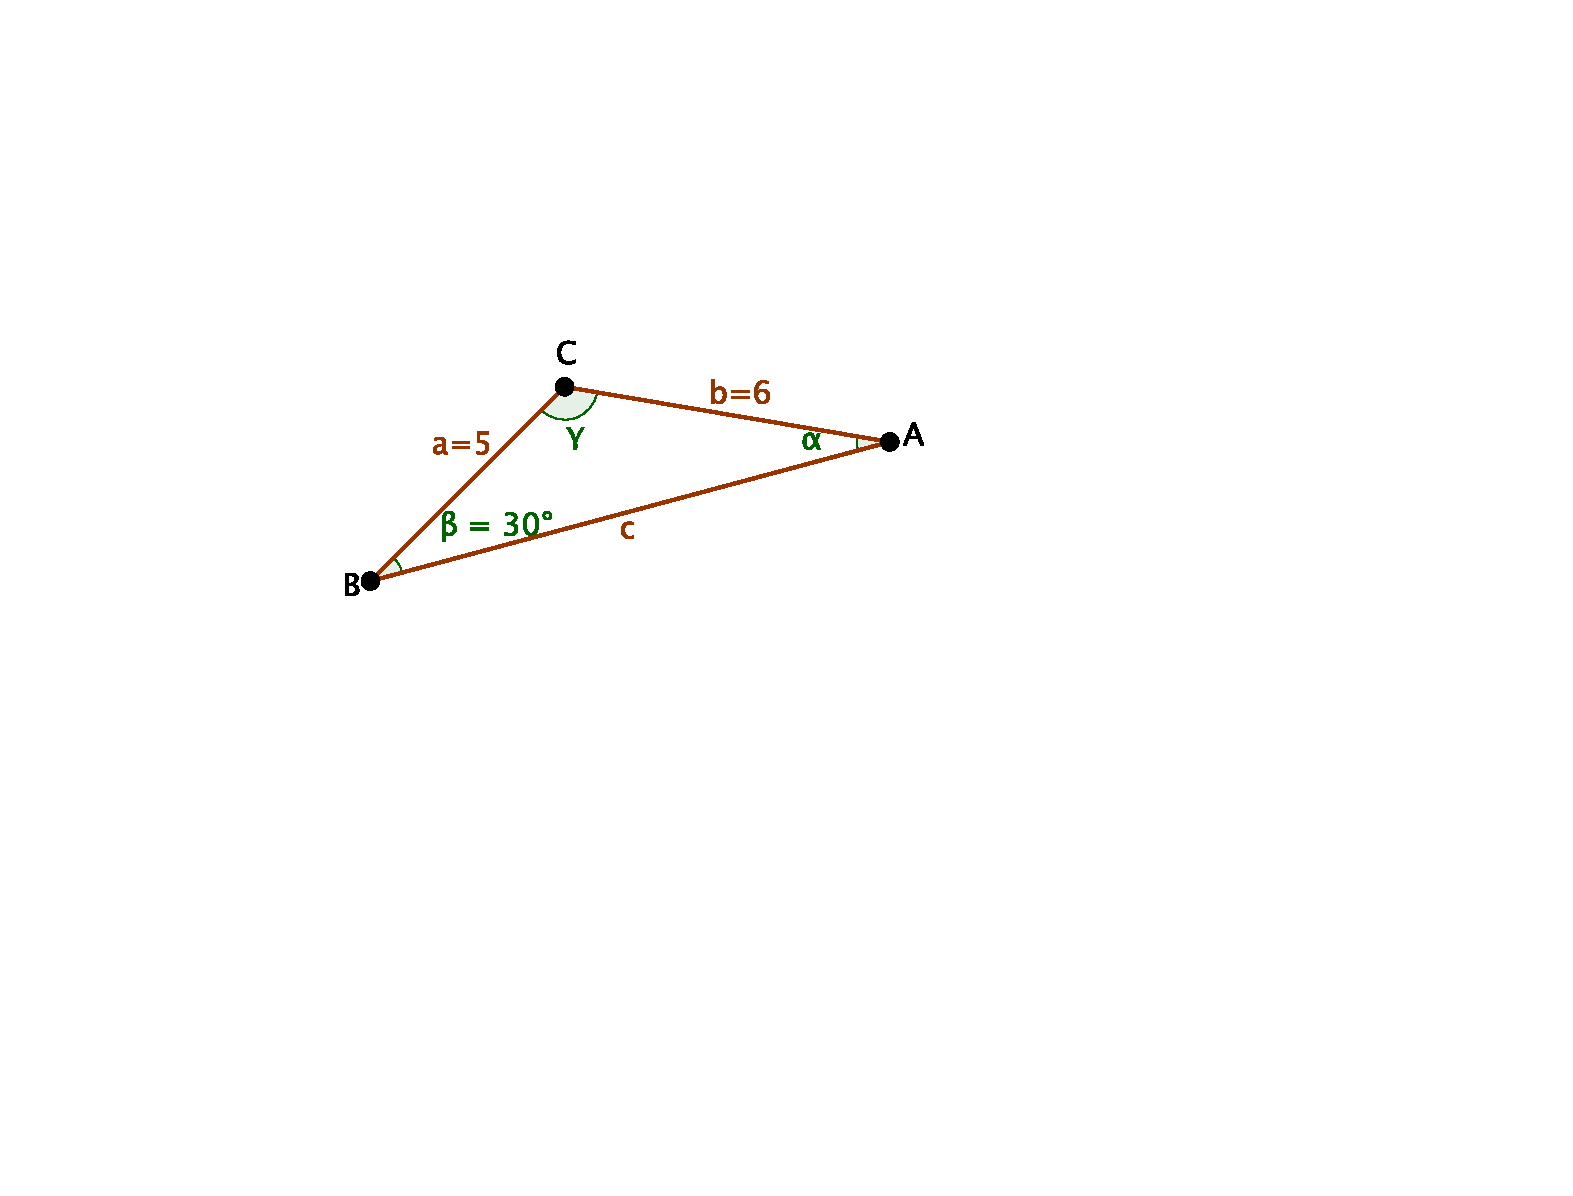
\includegraphics[width=0.9\textwidth]{img-03/trig-sample-triangle}
	
	{\footnotesize a) Representa els triangles deixant clares les dades i les incògnites.}
\end{minipage}
	\answers[cols=1]{[
 $A=24.52$; $C=125.38$; $c=9.78$,
$B=75$; $a=14.64$; $c=17.93$,
 No existeix cap triangle,
$A=77.36$; $B=C=51.32$,
Solució 1: $B=62.1$; $C=72.9$; $c=54.1$. 
Solució 2: $B=117.9$; $C=17.1$; $c=16.64$.]}x
	
	\exer
	Calcula l'àrea i el perímetre d'un pentàgon regular inscrit en una
	circumferència de radi 3 cm.
	
	\answers{El costat del polígon és $c=3.53$ cm  i l'apotema $a_p=2,43$  i l'àrea $A=21.4$ cm$^2$.\par 	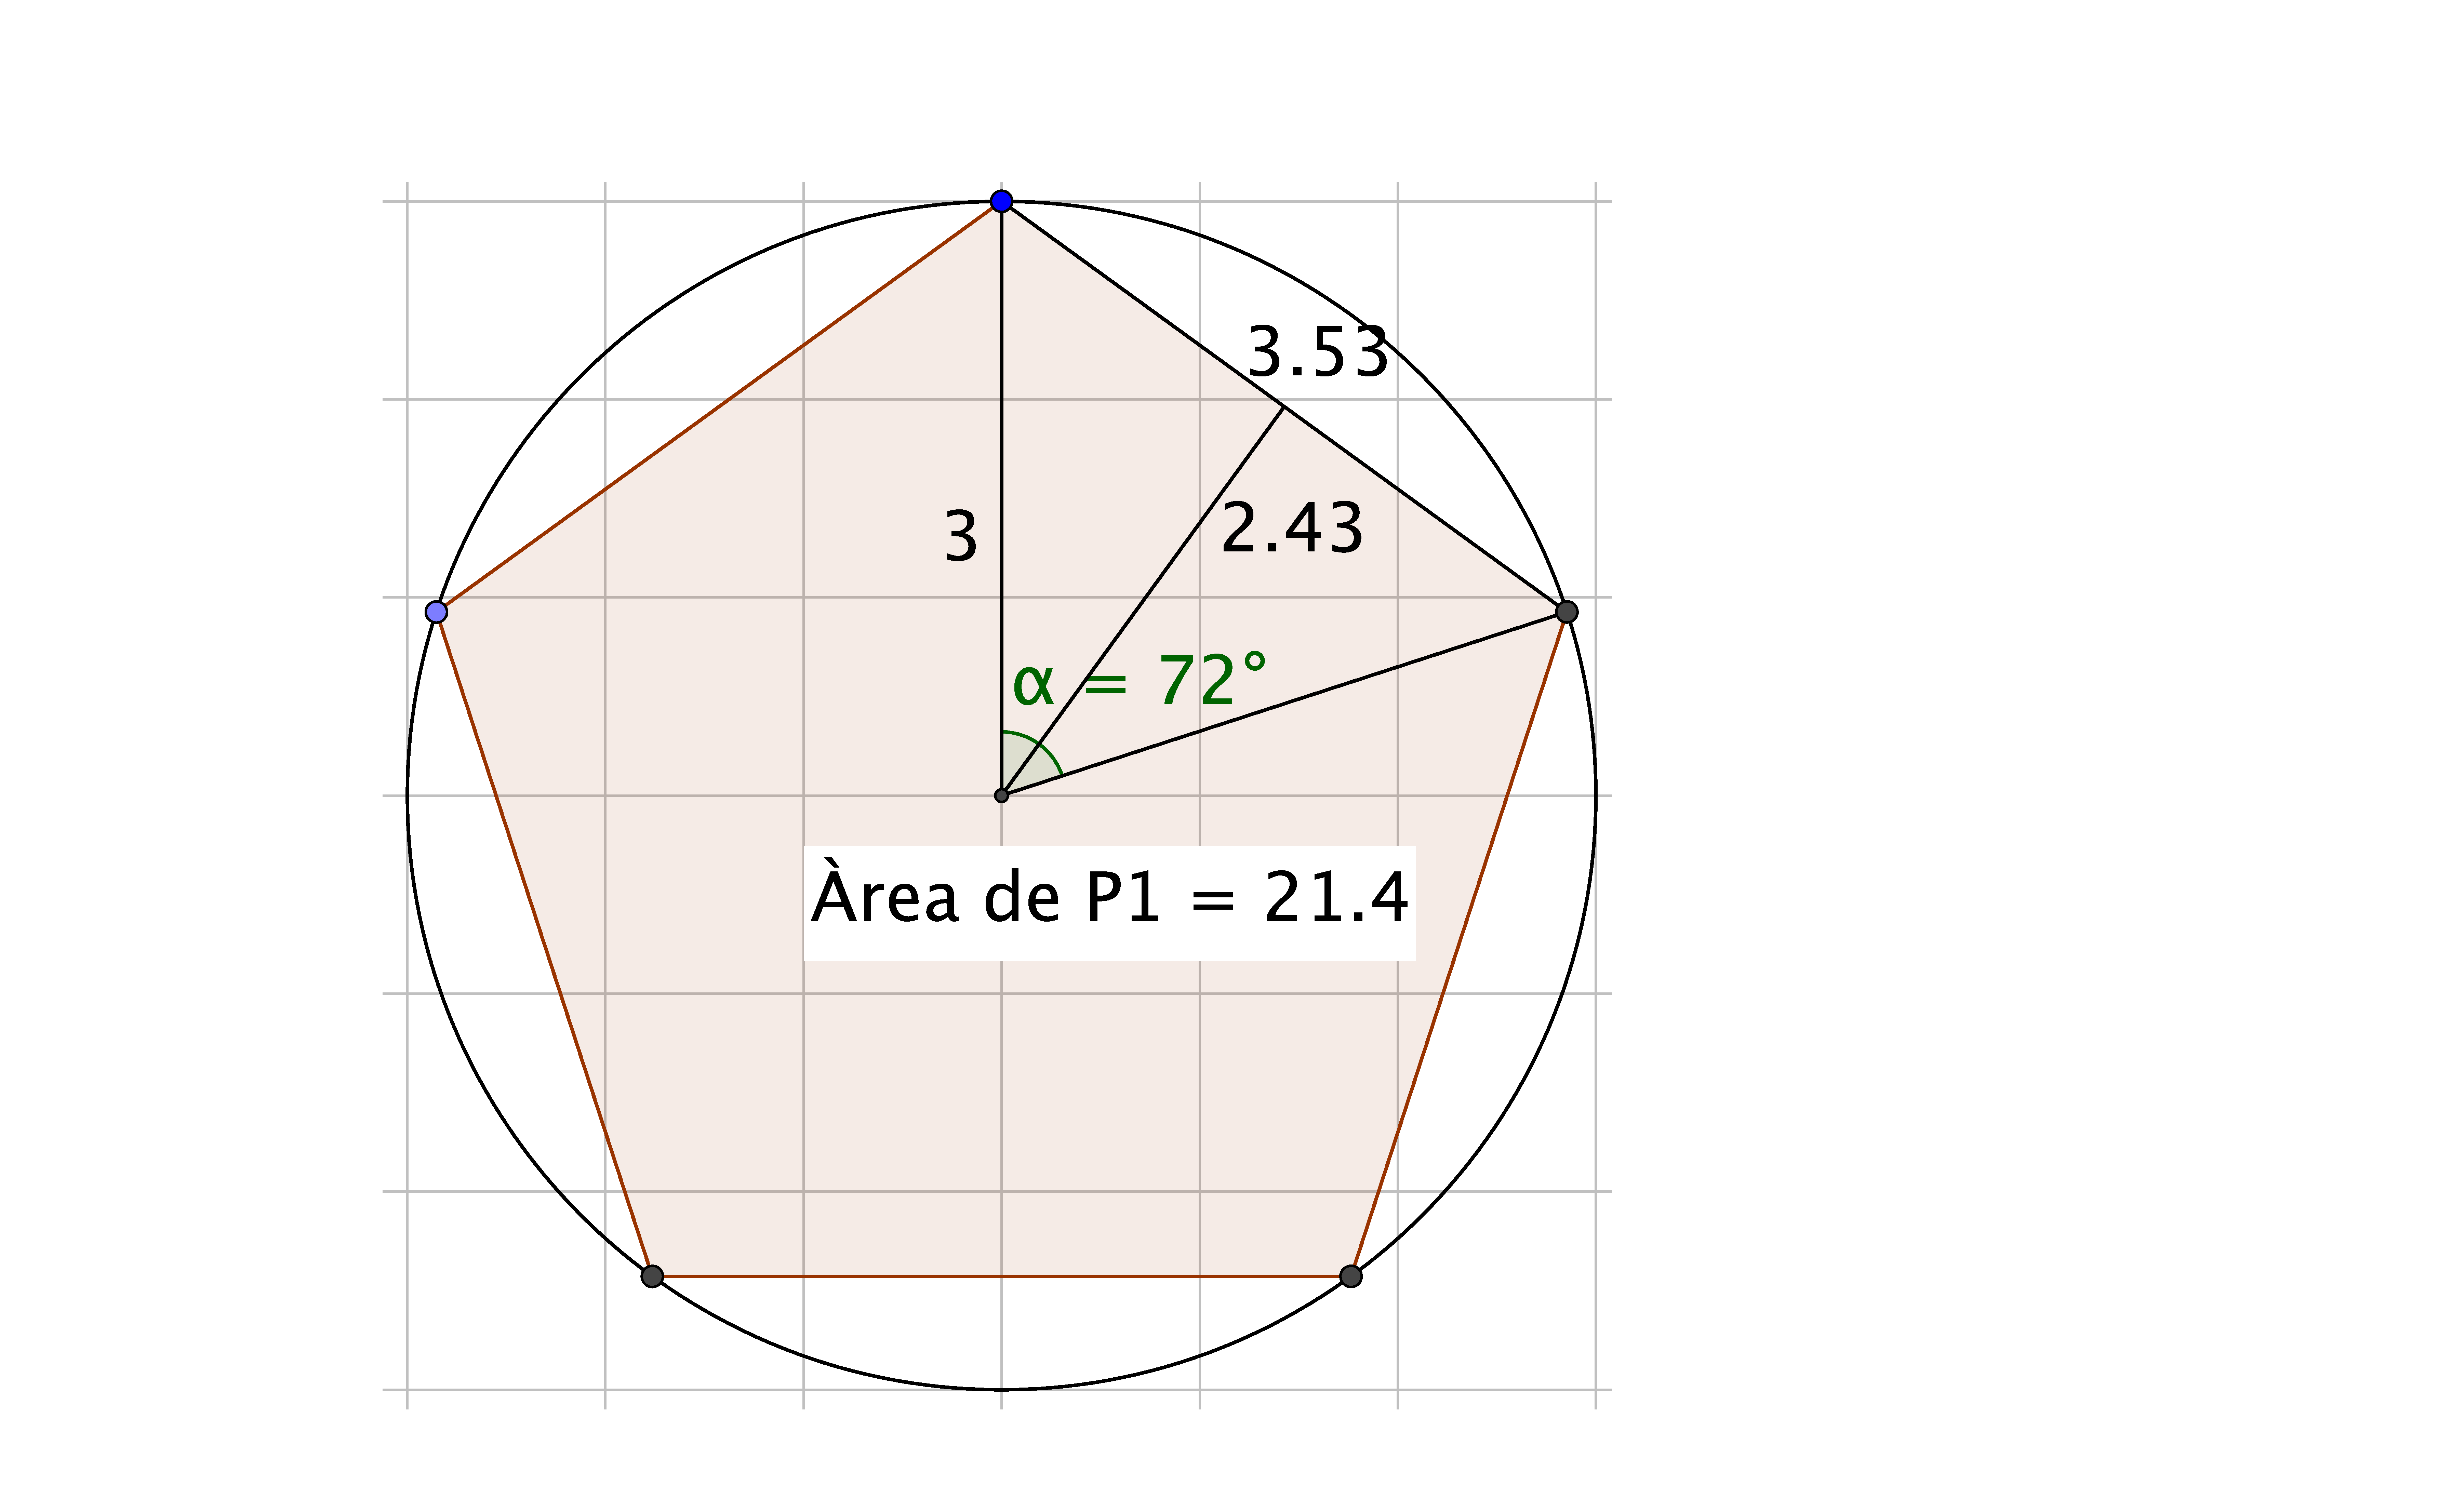
\includegraphics[width=0.3\textwidth]{img-sol/t3-36}}
	
	\pagebreak
	
	\exer
	Des d'un far \emph{F} es veu un vaixell A amb angle de 43${}^\circ$ amb la
	costa, i el vaixell B amb 21${}^\circ$. El vaixell \emph{B} està a 3 km de la
	costa i el A a 5 km. Calcula distància entre els vaixells.
	\begin{center}
		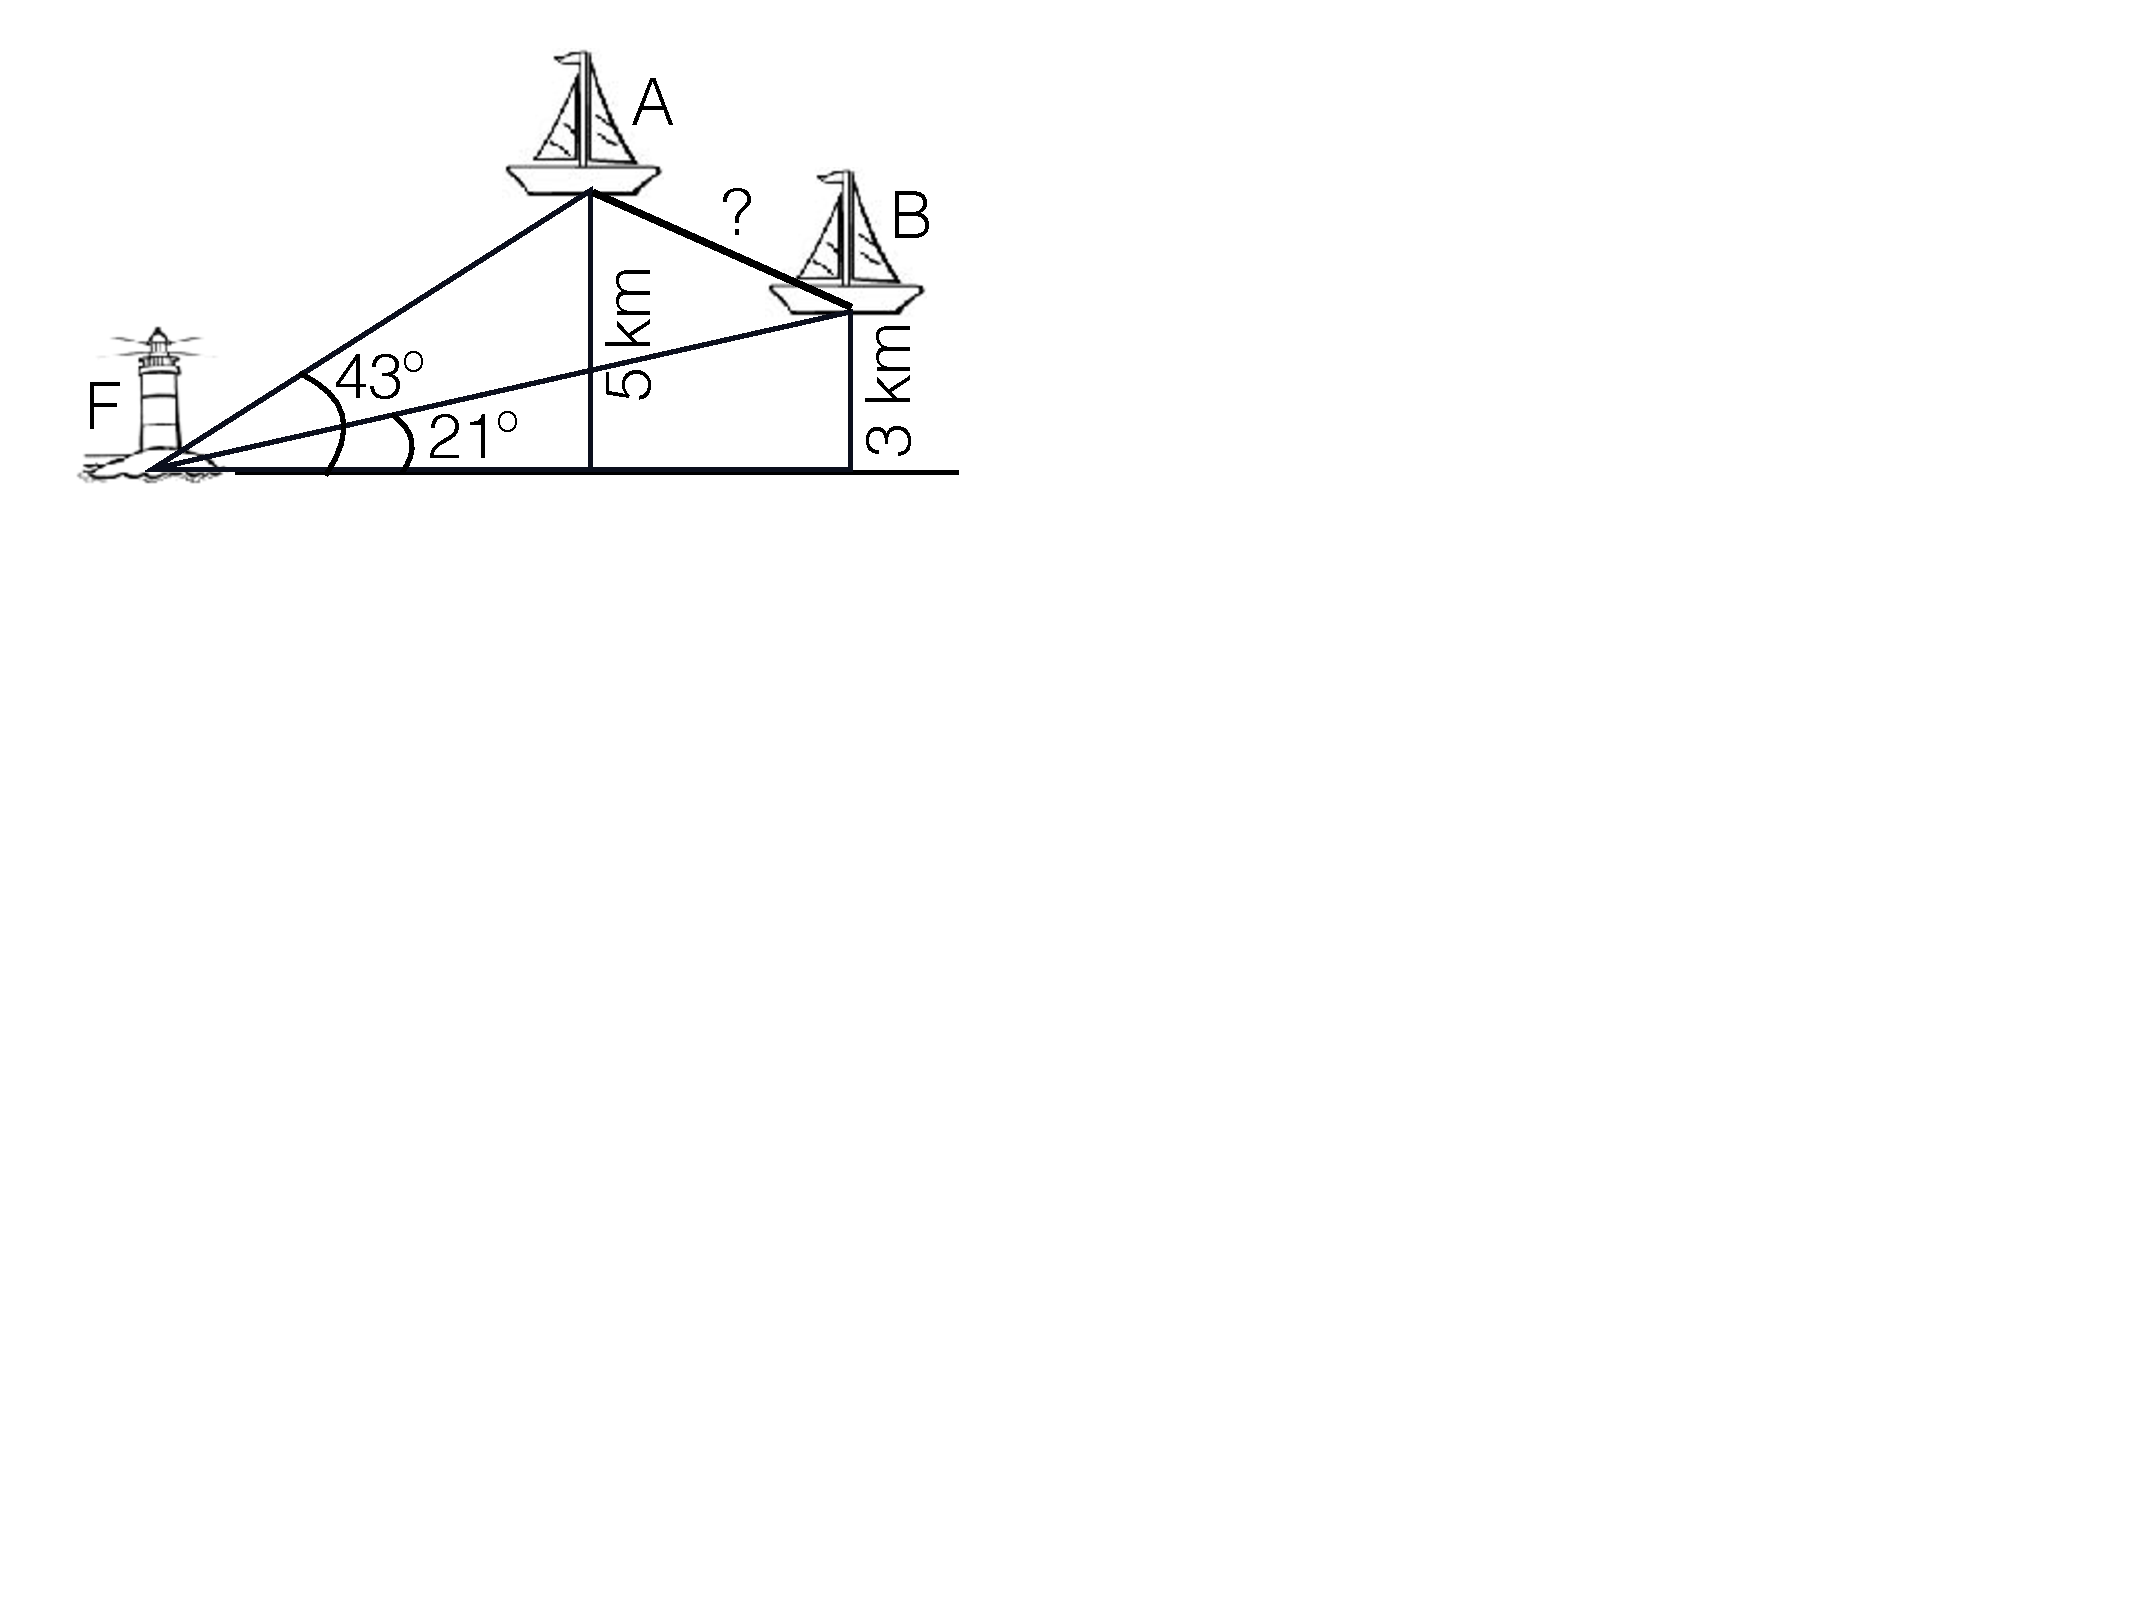
\includegraphics[width=5.1cm]{img-03/far}
	\end{center}
	
	\answers{Construïm el triangle rectangle de la figura. Té de catets $c=5-3=2$ i $b=\dfrac{3}{\tg 21} - \dfrac{5}{\tg 43}=2.453$. La distància és la hipotenusa del triangle $a=\sqrt{b^2+c^2}=3.165$ km 
		\par
			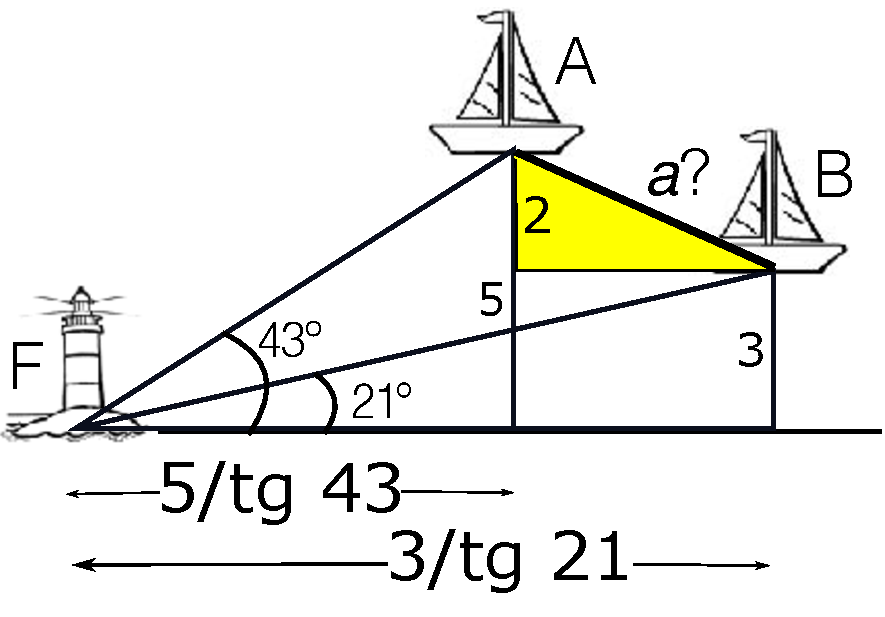
\includegraphics[width=0.4\textwidth]{img-sol/t3-37}
	}
	
	\exer
	Una finca té forma triangular. Dos dels seus costats mesuren 140 m i
	200 m respectivament, i l'angle comprès entre tots dos és de 35${}^\circ$.
	Calcula el perímetre i la superfície de la finca.
		\answers{Perímetre: 457.16 m. Àrea: 8030,1 m$^2$. 
		\par
		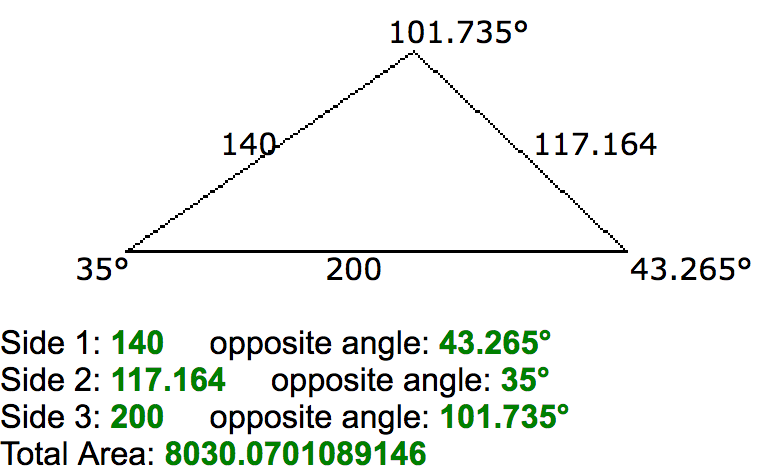
\includegraphics[width=0.42\textwidth]{img-sol/t3-38}
	}
	
	\exer
	Calcula l'altura de la torre: 
	\begin{center}
		\vspace{-1cm}
		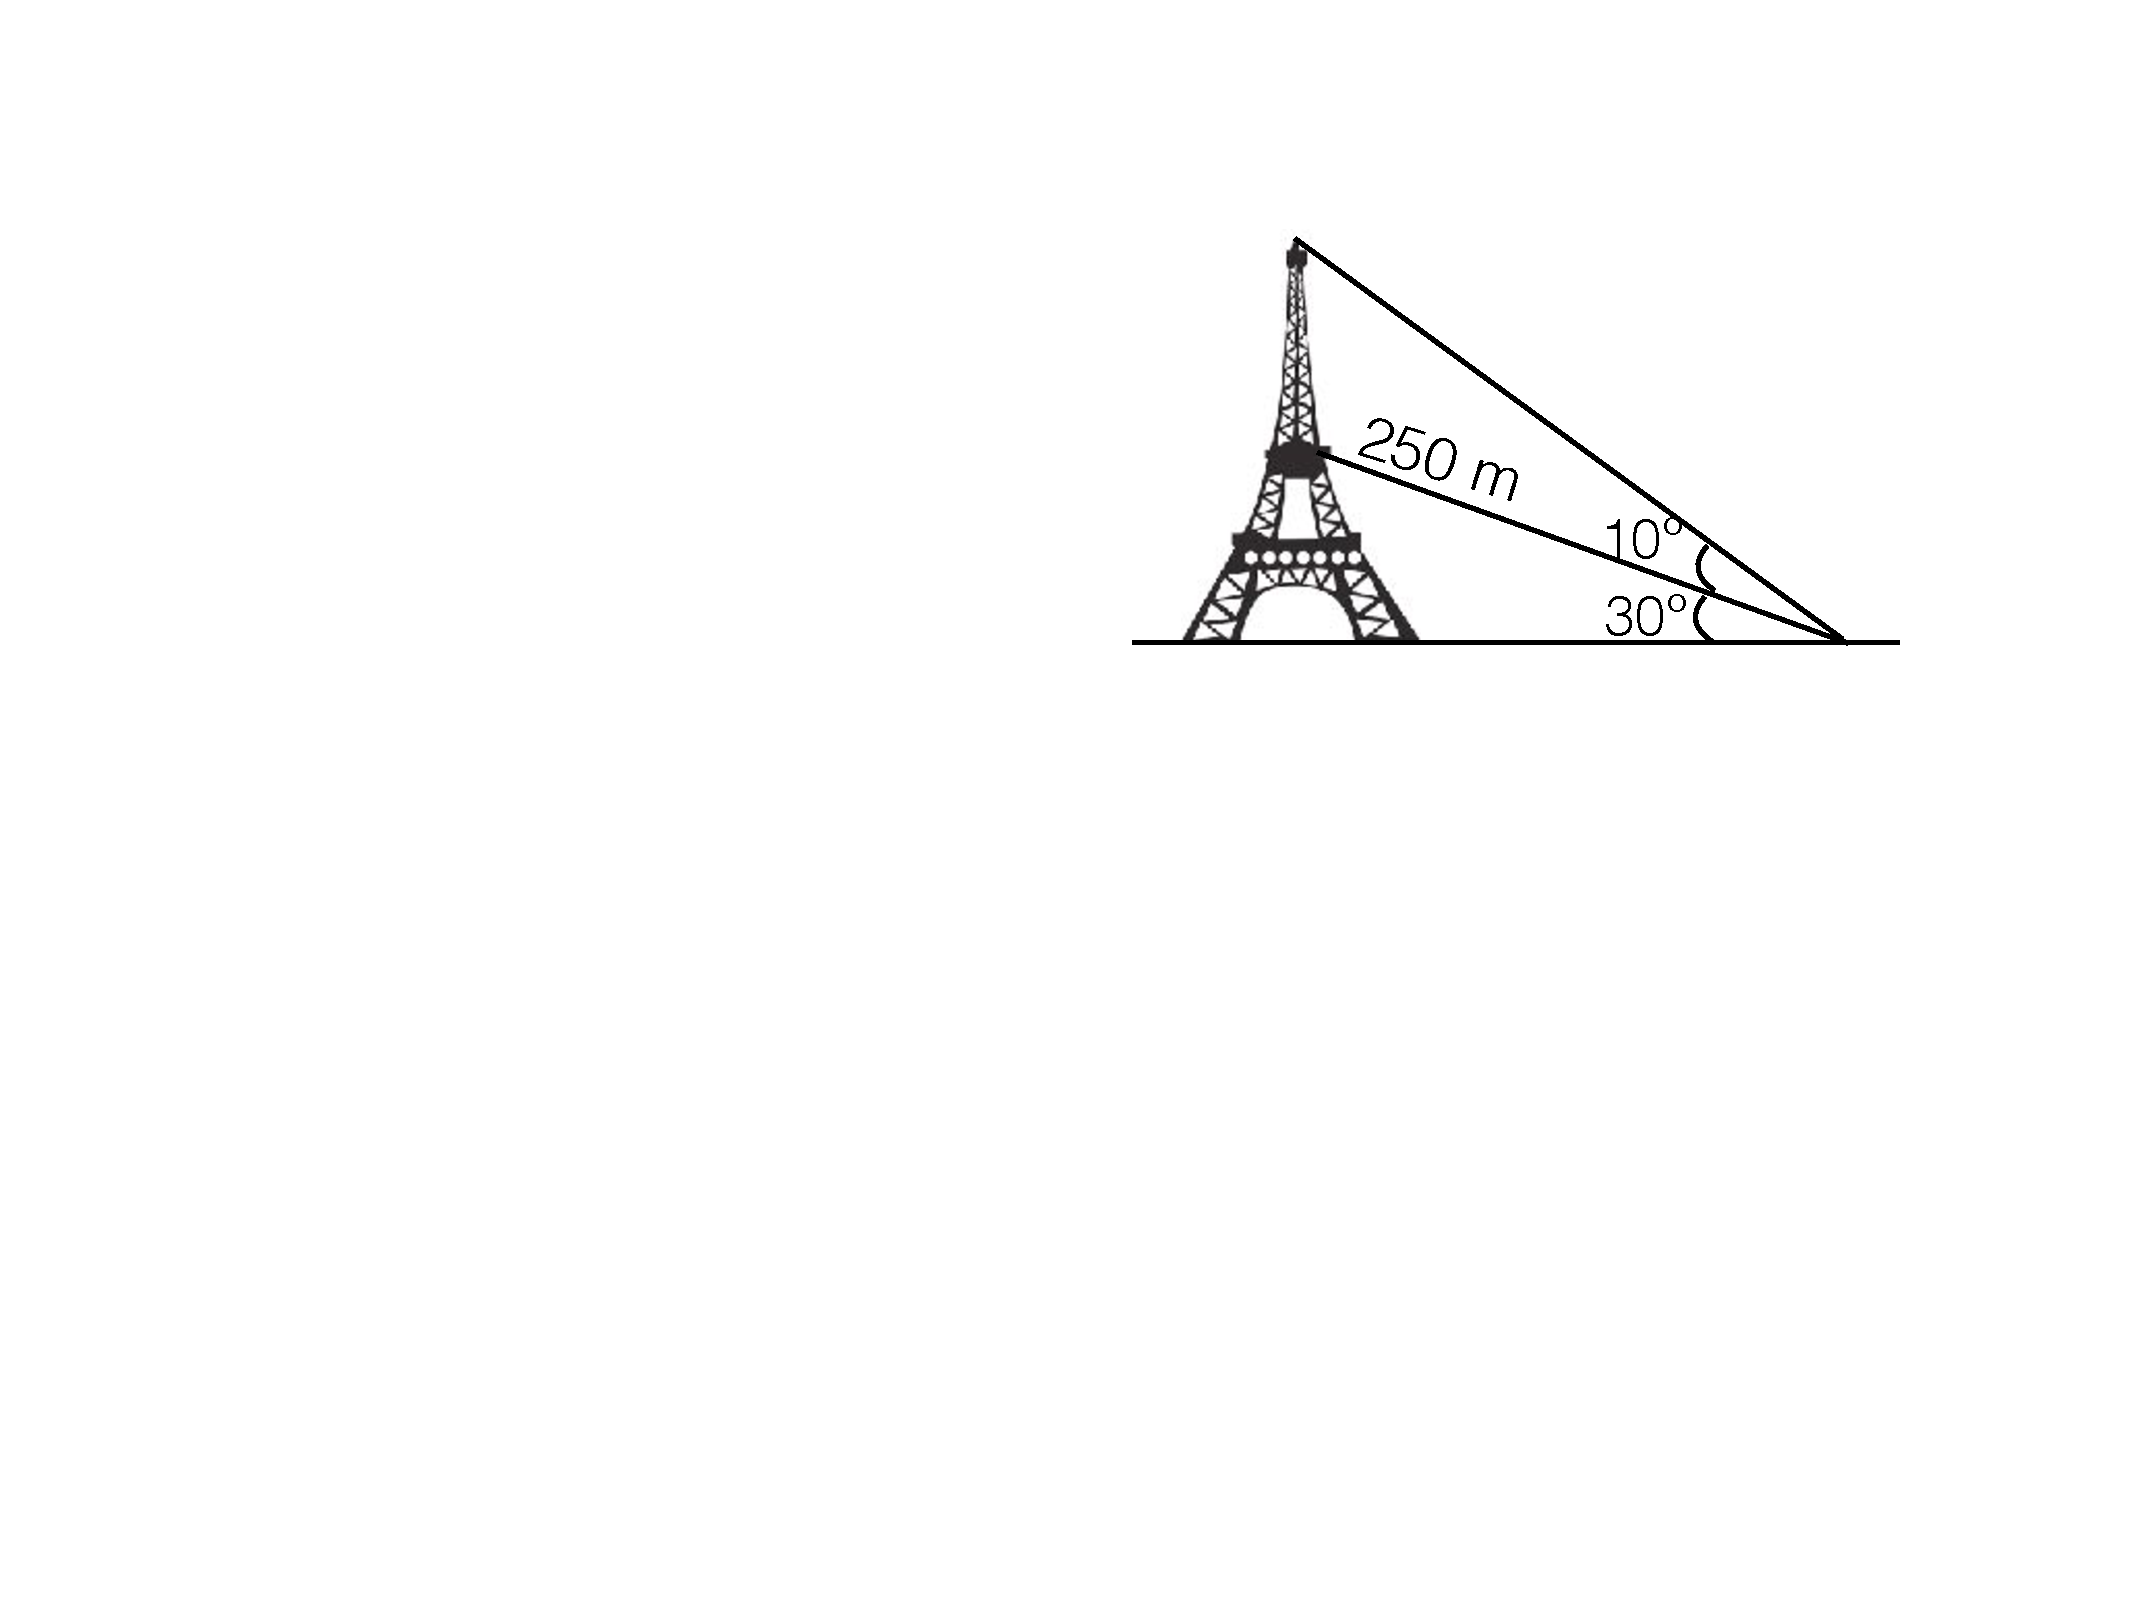
\includegraphics[width=5cm]{img-03/edifici}
	\end{center}

	\answers{Del triangle rectangle d'abaix trobam la base com $b=250\cos 30=216.51$ m. Del triangle rectangle complet $\tg 40 = \dfrac{H}{216.51}$, aïllam $H=181.67$ m.}
	
	\exer
	Dues persones \emph{A} \emph{i B} disten entre sí 200 m i veuen un
	globus que està situat entre ambdues. La primera persona ho veu amb un
	angle de 30${}^\circ$ i la segona amb un angle de 60${}^\circ$.
	
	\begin{tasks}
		\task
		A quina distància està \emph{B} del globus?
		\task
		A quina altura està el globus?
		\task
		Una persona que estigui situada dins del globus, amb quin angle veu
		a \emph{A} i \emph{B}?
	\end{tasks}
\answers[cols=3]{[100 m, 86.60 m, 90$^\circ$]}
	
	\exer
	\begin{minipage}[t]{0.55\textwidth}
		Calcula l'altura de la torre gran a partir del següent dibuix.
	\end{minipage}\hfill
	\begin{minipage}[t]{5.5cm}
		\vspace{-\baselineskip}
		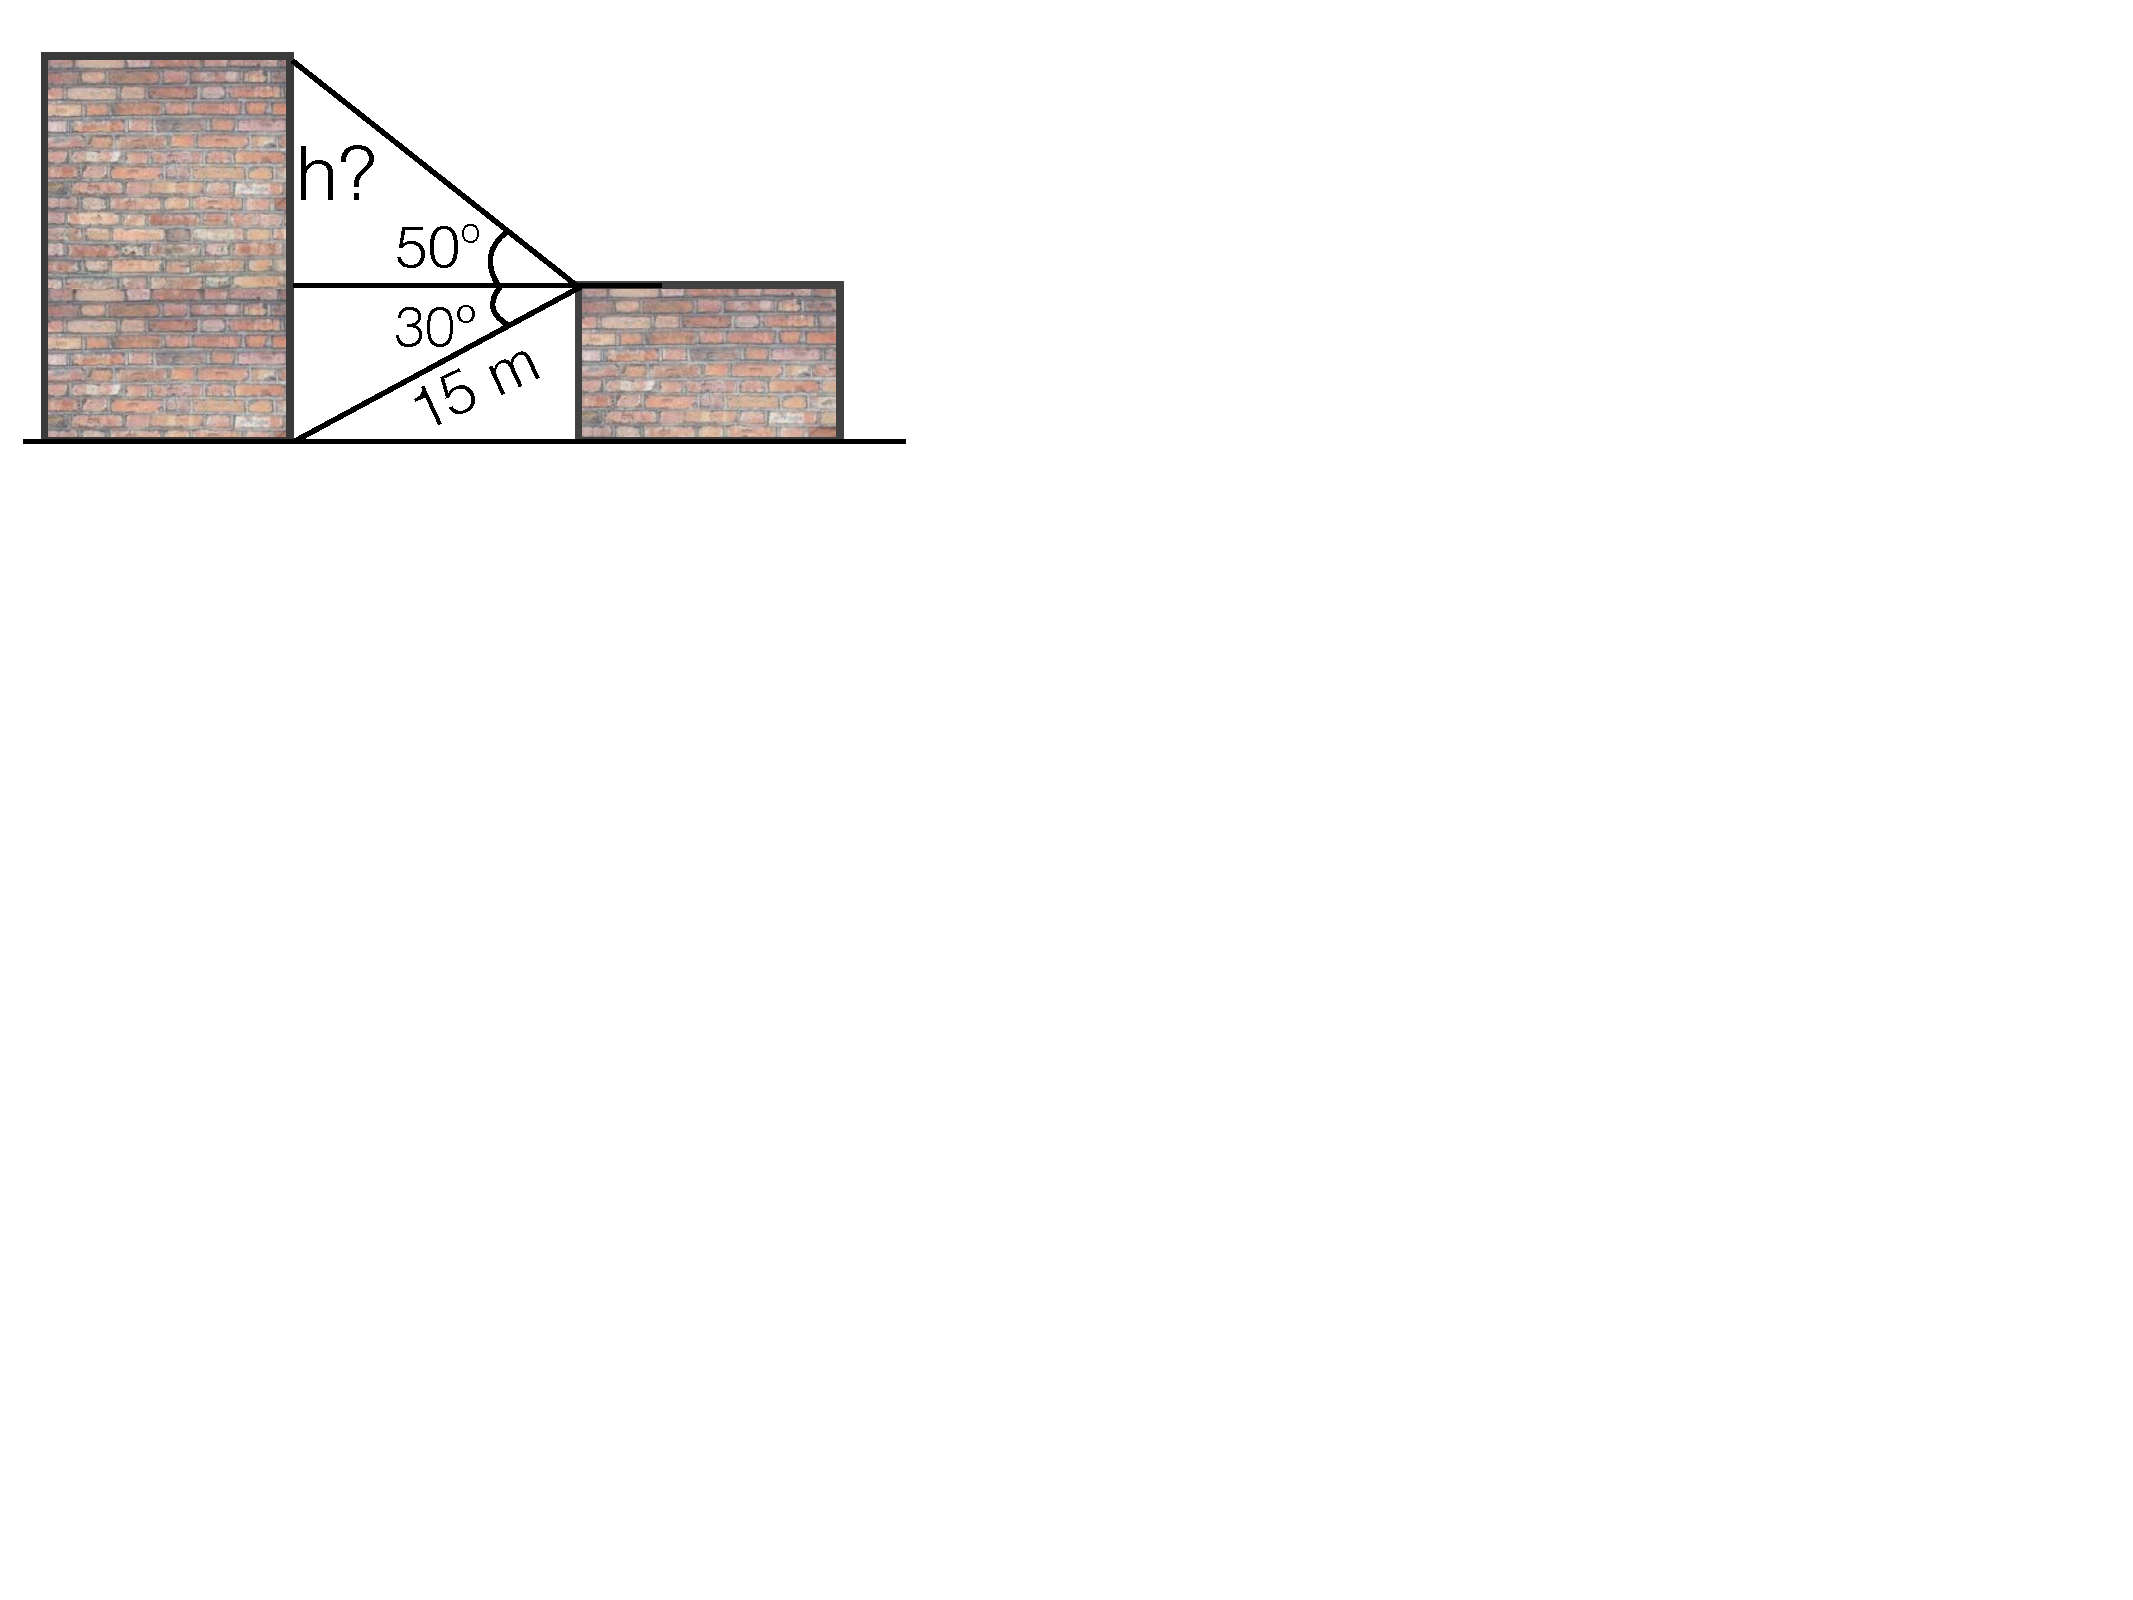
\includegraphics[width=5cm]{img-03/torre}
	\end{minipage}

	\answers{Primer trobam els angles que falten. Es un triangle d'angles 80, 60, 40. Aplicam el teorema del sinus: $\dfrac{h}{\sin 80}=\dfrac{15}{\sin 40}$. Aïllam $h =22.98$ m.}
	
	
	\exer
	Desitgem mesurar l'altura d'un edifici. Si ho observem des d'un punt
	\emph{A} ho veiem amb un angle de 50${}^\circ$. Ara bé, si ho contemplem des de
	20 m més lluny \emph{B}, l'angle és de 40${}^\circ$. Quina és l'altura de l'edifici? A
	quina distància està el punt \emph{B} d'aquest edifici?
	\answers{$d(B, E) = 67.59$; $h = 56,7135$ m}
	
	
	\exer
	Comencem en una ciutat \emph{A} i observem un cartell. La ciutat
	\emph{B} està a 50 Km i la ciutat \emph{C} a 40 Km. Mesurem l'angle
	que formen les dues carreteres i resulta ser de 60${}^\circ$. A quina distància
	està \emph{B} de C ? Des de la ciutat \emph{B}, amb quin angle es veuen
	les altres dues ciutats? {[}En altres paraules: si considerem el
	triangle \emph{ABC,} què val l'angle que correspon al vèrtex
	\emph{B}?{]}
	
	\answers{Des de $B$ les altres dues ciutats es veuen amb un angle de  49.11$^\circ$.
		\par
		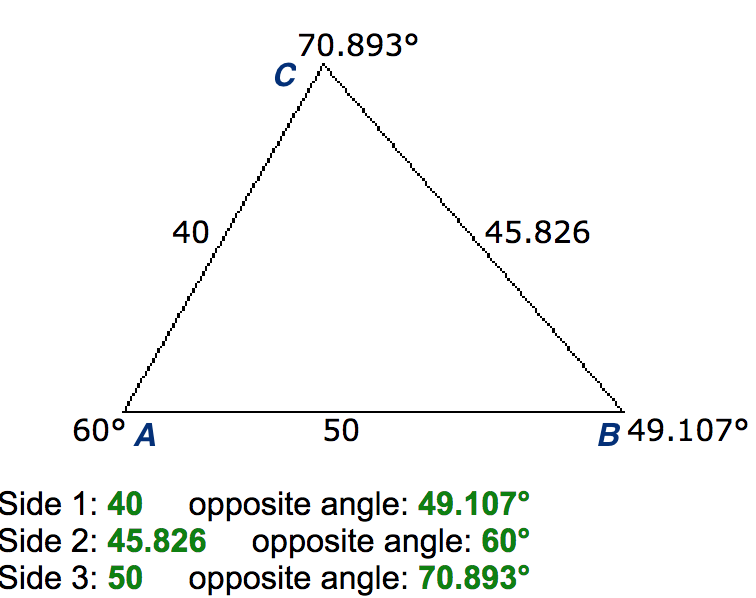
\includegraphics[width=0.43\textwidth]{img-sol/t3-43}}
	
	
	\exer[1] Per determinar l'amplada d'un riu ens fixam amb un 
	arbre que està situat en un punt C de la vorera. Arran de l'altra vorera
	hi ha dues cases A i B separades 30 m. Des de la casa A, l'arbre i la casa B
	formen un angle de 60${}^\circ$. Des de la casa B, l'angle que forma l'arbre i la casa A 
	és de 75${}^\circ$. Calcula l'amplada del riu. 
	\answers{$d=35,49$ m}
	
	\exer[-1]
	\begin{minipage}[t]{0.55\textwidth}
		\spicy  A i B són dues ciutats situades a l'altra banda d'un riu de pas 
		inaccessible. Aquestes ciutats, però, són visibles des d'altres punts accessibles
		C i D, separats per una distància de 73,2 km. Sabent els angles
		$\widehat{ACD}=80,2^\circ$, $\widehat{BCD}=43,5^\circ$, $\widehat{ADC}=23,23^\circ$, $\widehat{BDC}=32^\circ$, determina la distància entre les dues ciutats AB.
	\end{minipage}\hfill
	\begin{minipage}[t]{5.5cm}
		\vspace{-\baselineskip}
		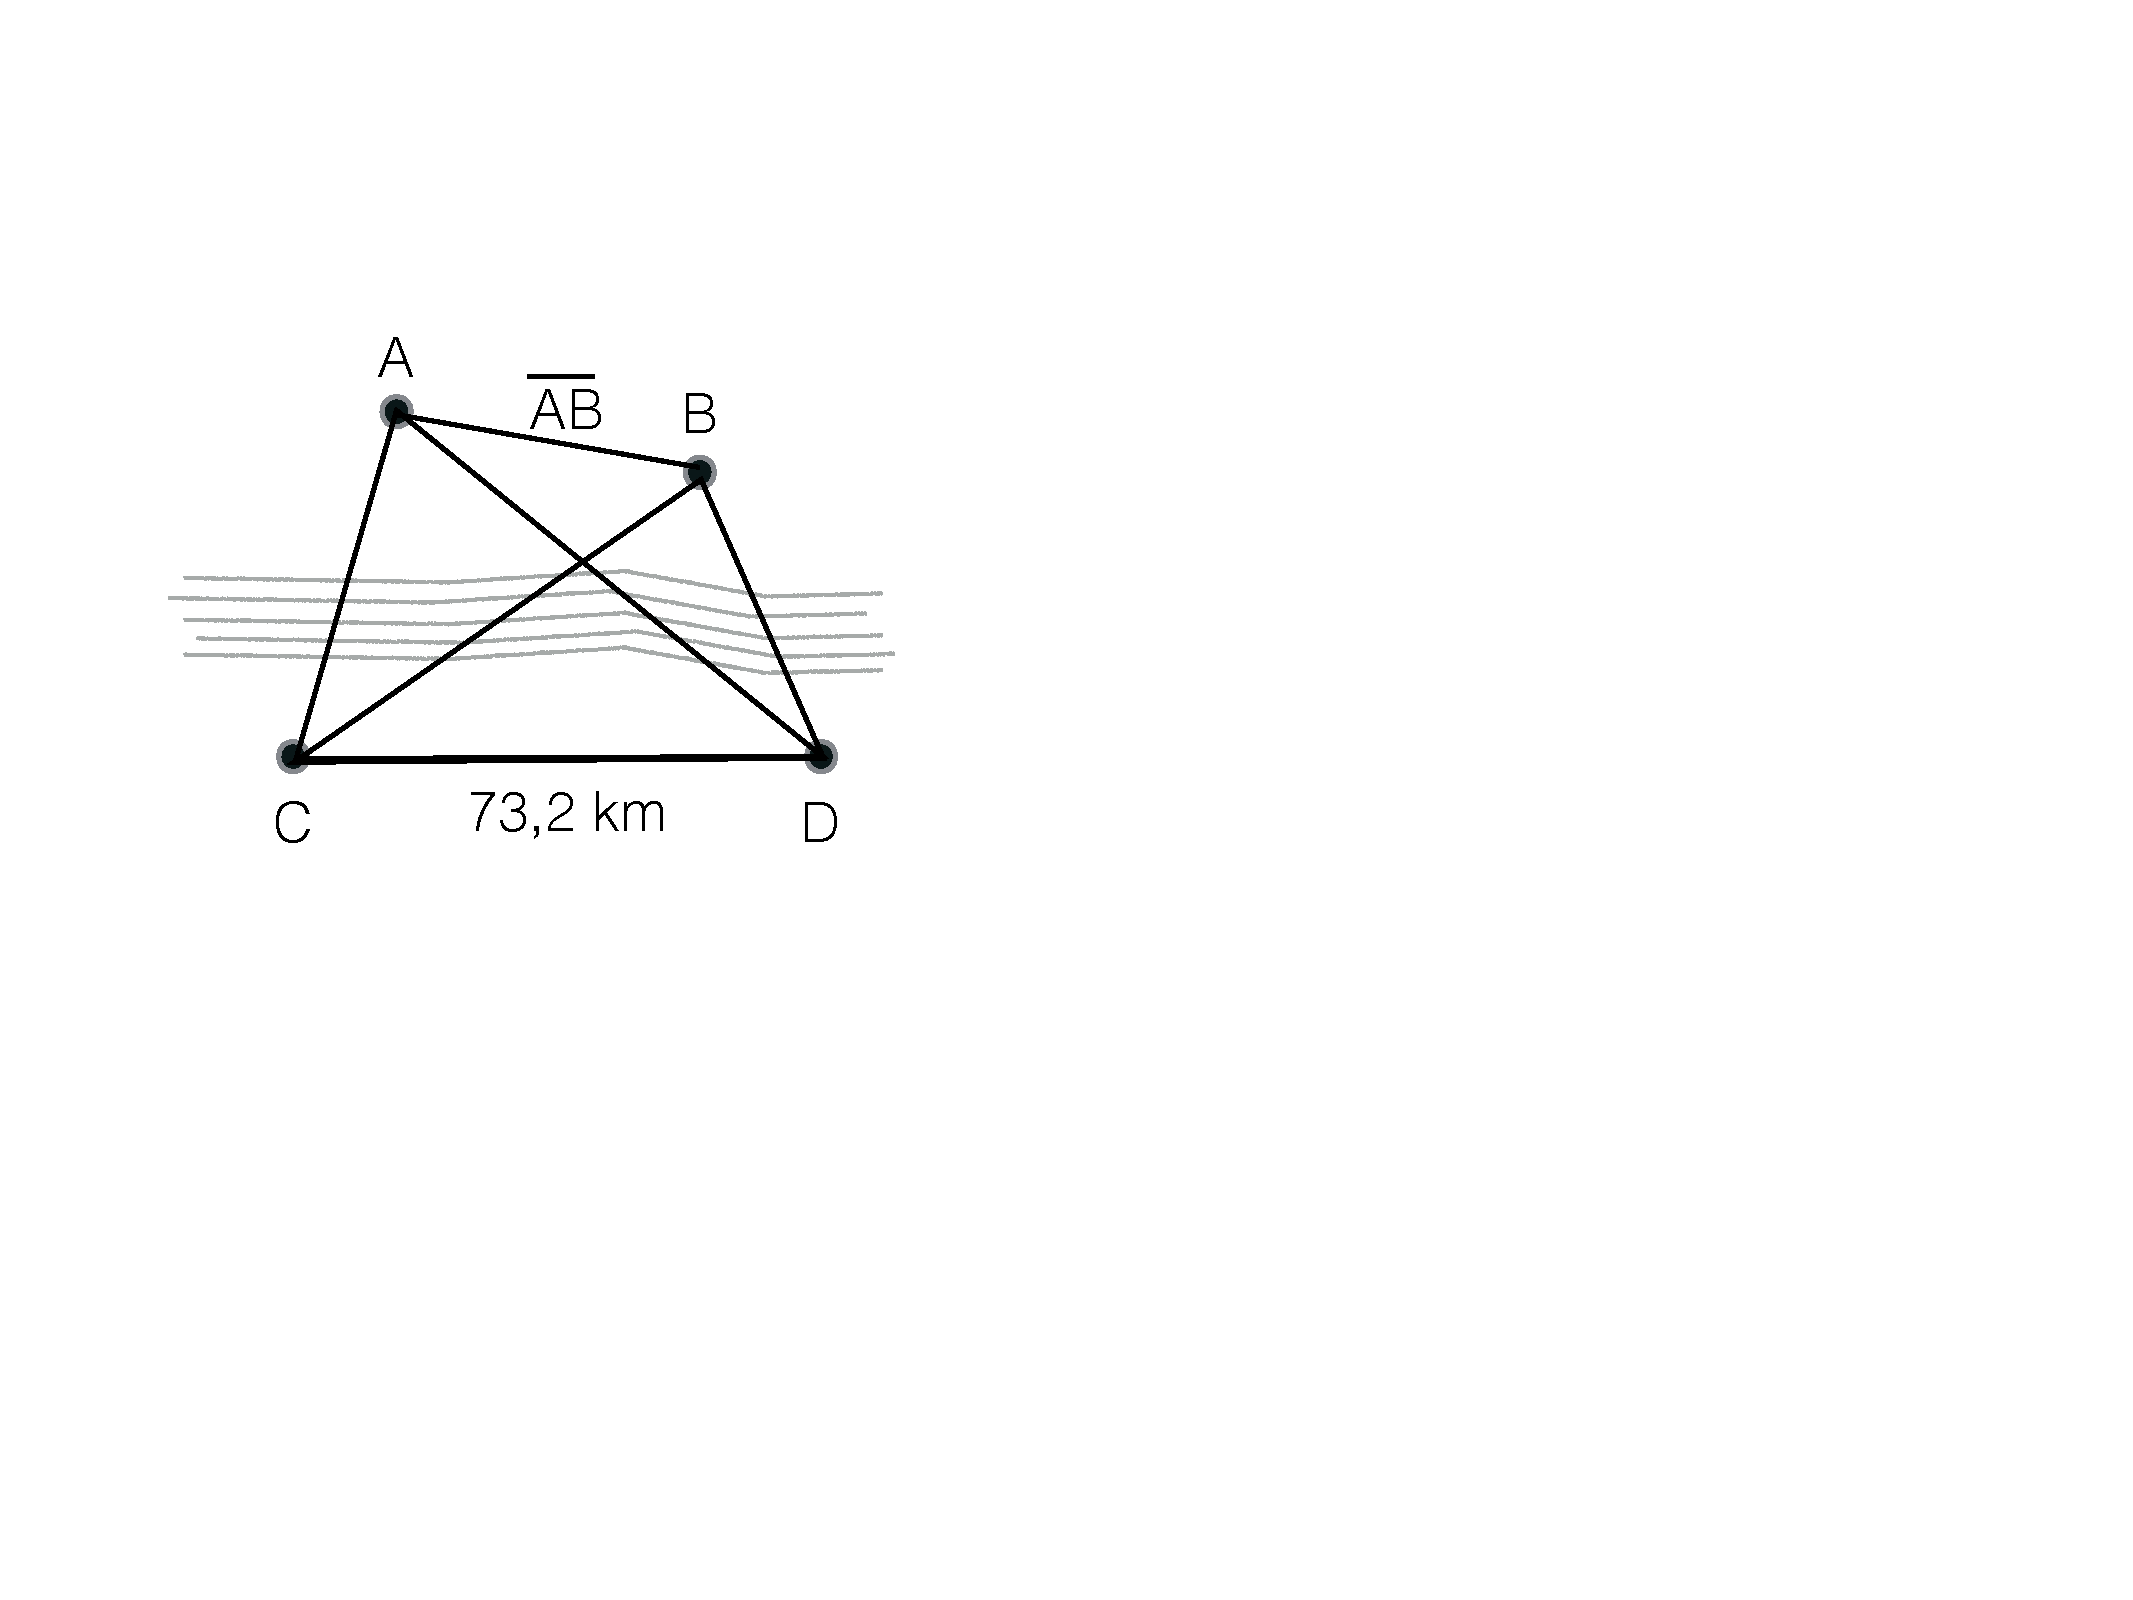
\includegraphics[width=5cm]{img-03/ciutats}
	\end{minipage}
	\answers{Del triangle $\widehat{CAD}$ troba $\overline{AD}=74.16$ km, del triangle $\widehat{CBD}$ troba $\overline{BD}=52.05$ km pel teorema del sinus i finalment del triangle $\widehat{ADB}$ troba  $\overline{AB}=24$ km pel teorema del cosinus.}
	
	\exer[1]
	\begin{minipage}[t]{0.55\textwidth}
		\spicy Dos muntanyistes que han pujat en caps de setmana successius a dos cims veïns volen saber quina és la
		distància entre aquests dos cims. Per això, han mesurat des del peu del cim A els angles d'elevació dels cims A i B que són 65${}^\circ$ i 30${}^\circ$, respectivament. 
	\end{minipage}\hfill
	\begin{minipage}[t]{5.5cm}
		\vspace{-\baselineskip}
		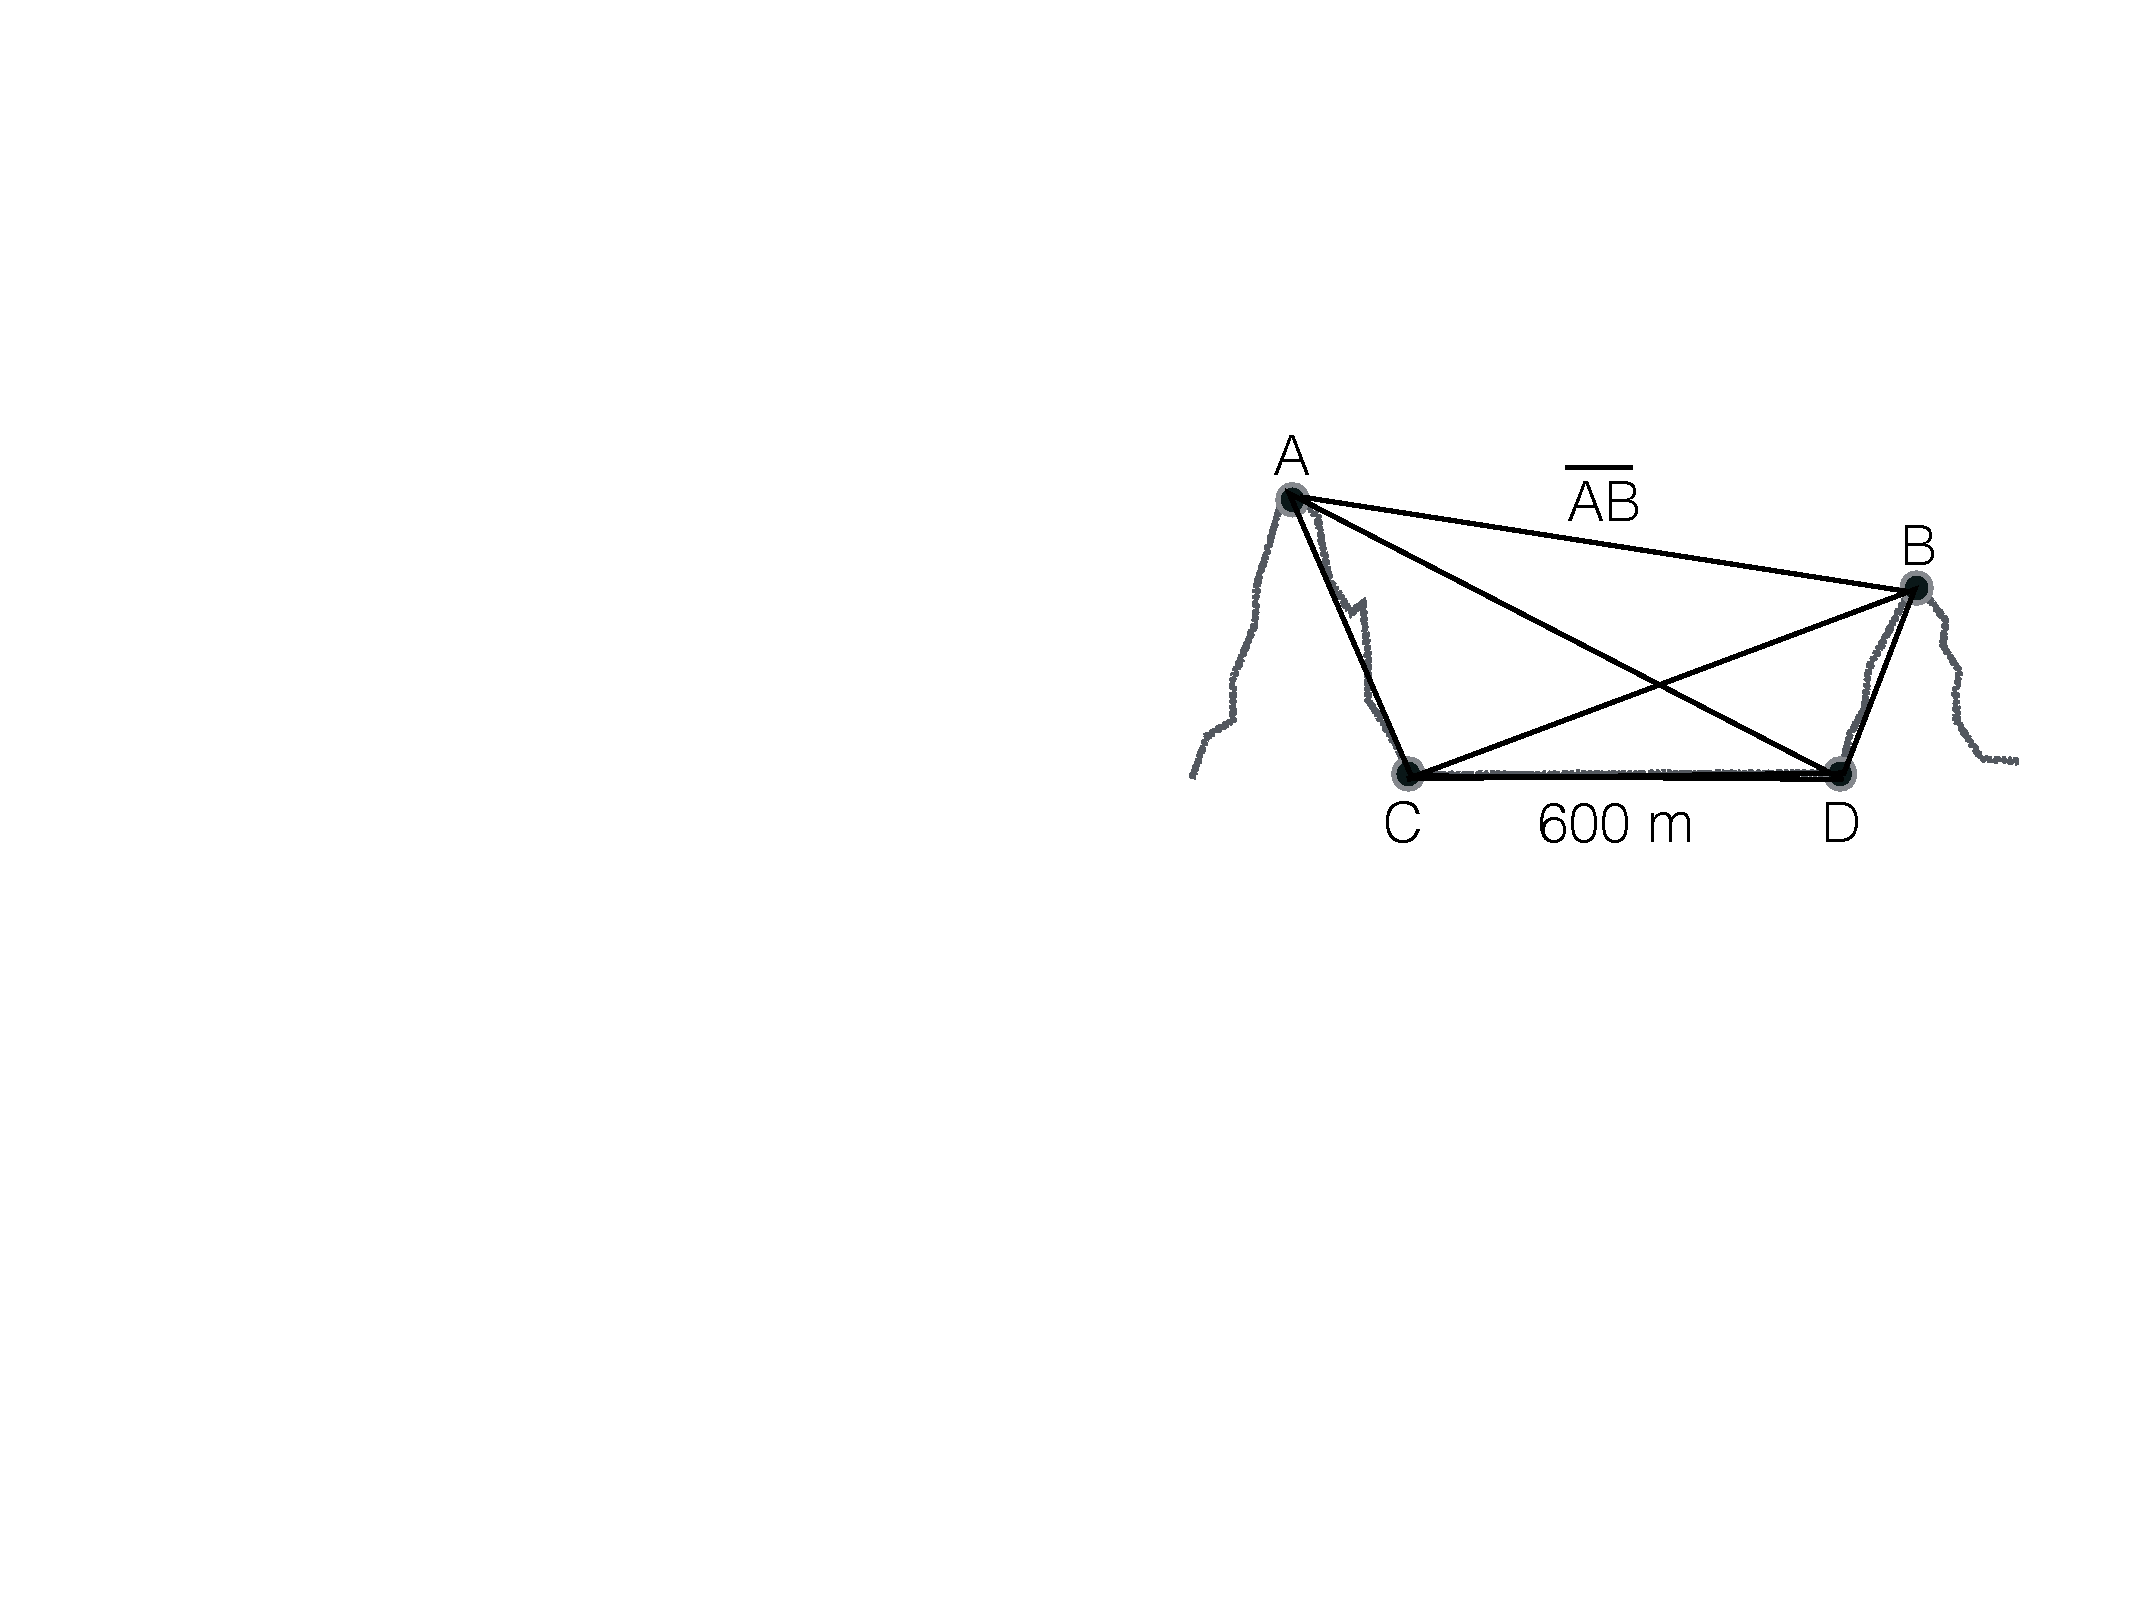
\includegraphics[width=5.3cm]{img-03/muntanyes}
	\end{minipage}
	
	Després han caminat fins el peu del cim B i han mesurat els angles d'elevació dels cims A i B de 40${}^\circ$ i 47${}^\circ$, respectivament. La distància entre els dos peus dels cims és de 600 m. Què val la distància entre els dos cims?
	\answers{cim A=827 m, cim B=751 m, distància entre cims AB=1687.2 m}

	\exer
	En un viatge d'alumnes de 4t d'ESO a Londres, alguns dels viatgers
	van fer pràctiques de trigonometria. En conèixer que
	l'Abadia de Westminster té una altura de 30 metres, van decidir
	aprofitar els seus coneixements per calcular l'altura de la famosa
	torre Big Ben. Des d'un punt situat entre els dos edificis
	s'observa el punt més alt de l'Abadia amb angle de 60$^\circ$, i el Big Ben
	amb un angle de 45$^\circ$. Si la distància entre les bases de les torres
	dels dos edificis és de 50 metres, quin va ser el resultat dels seus
	càlculs?, a quina distància es trobava de cada edifici?
	
	\answers{Es trobava a 17.32 m de l'Abadia de Westminster i a 32.68 m del Big Ben. L'altura del Big Ben és 32.68 m ja que es veu amb un angle de 45$^\circ$.
	\par 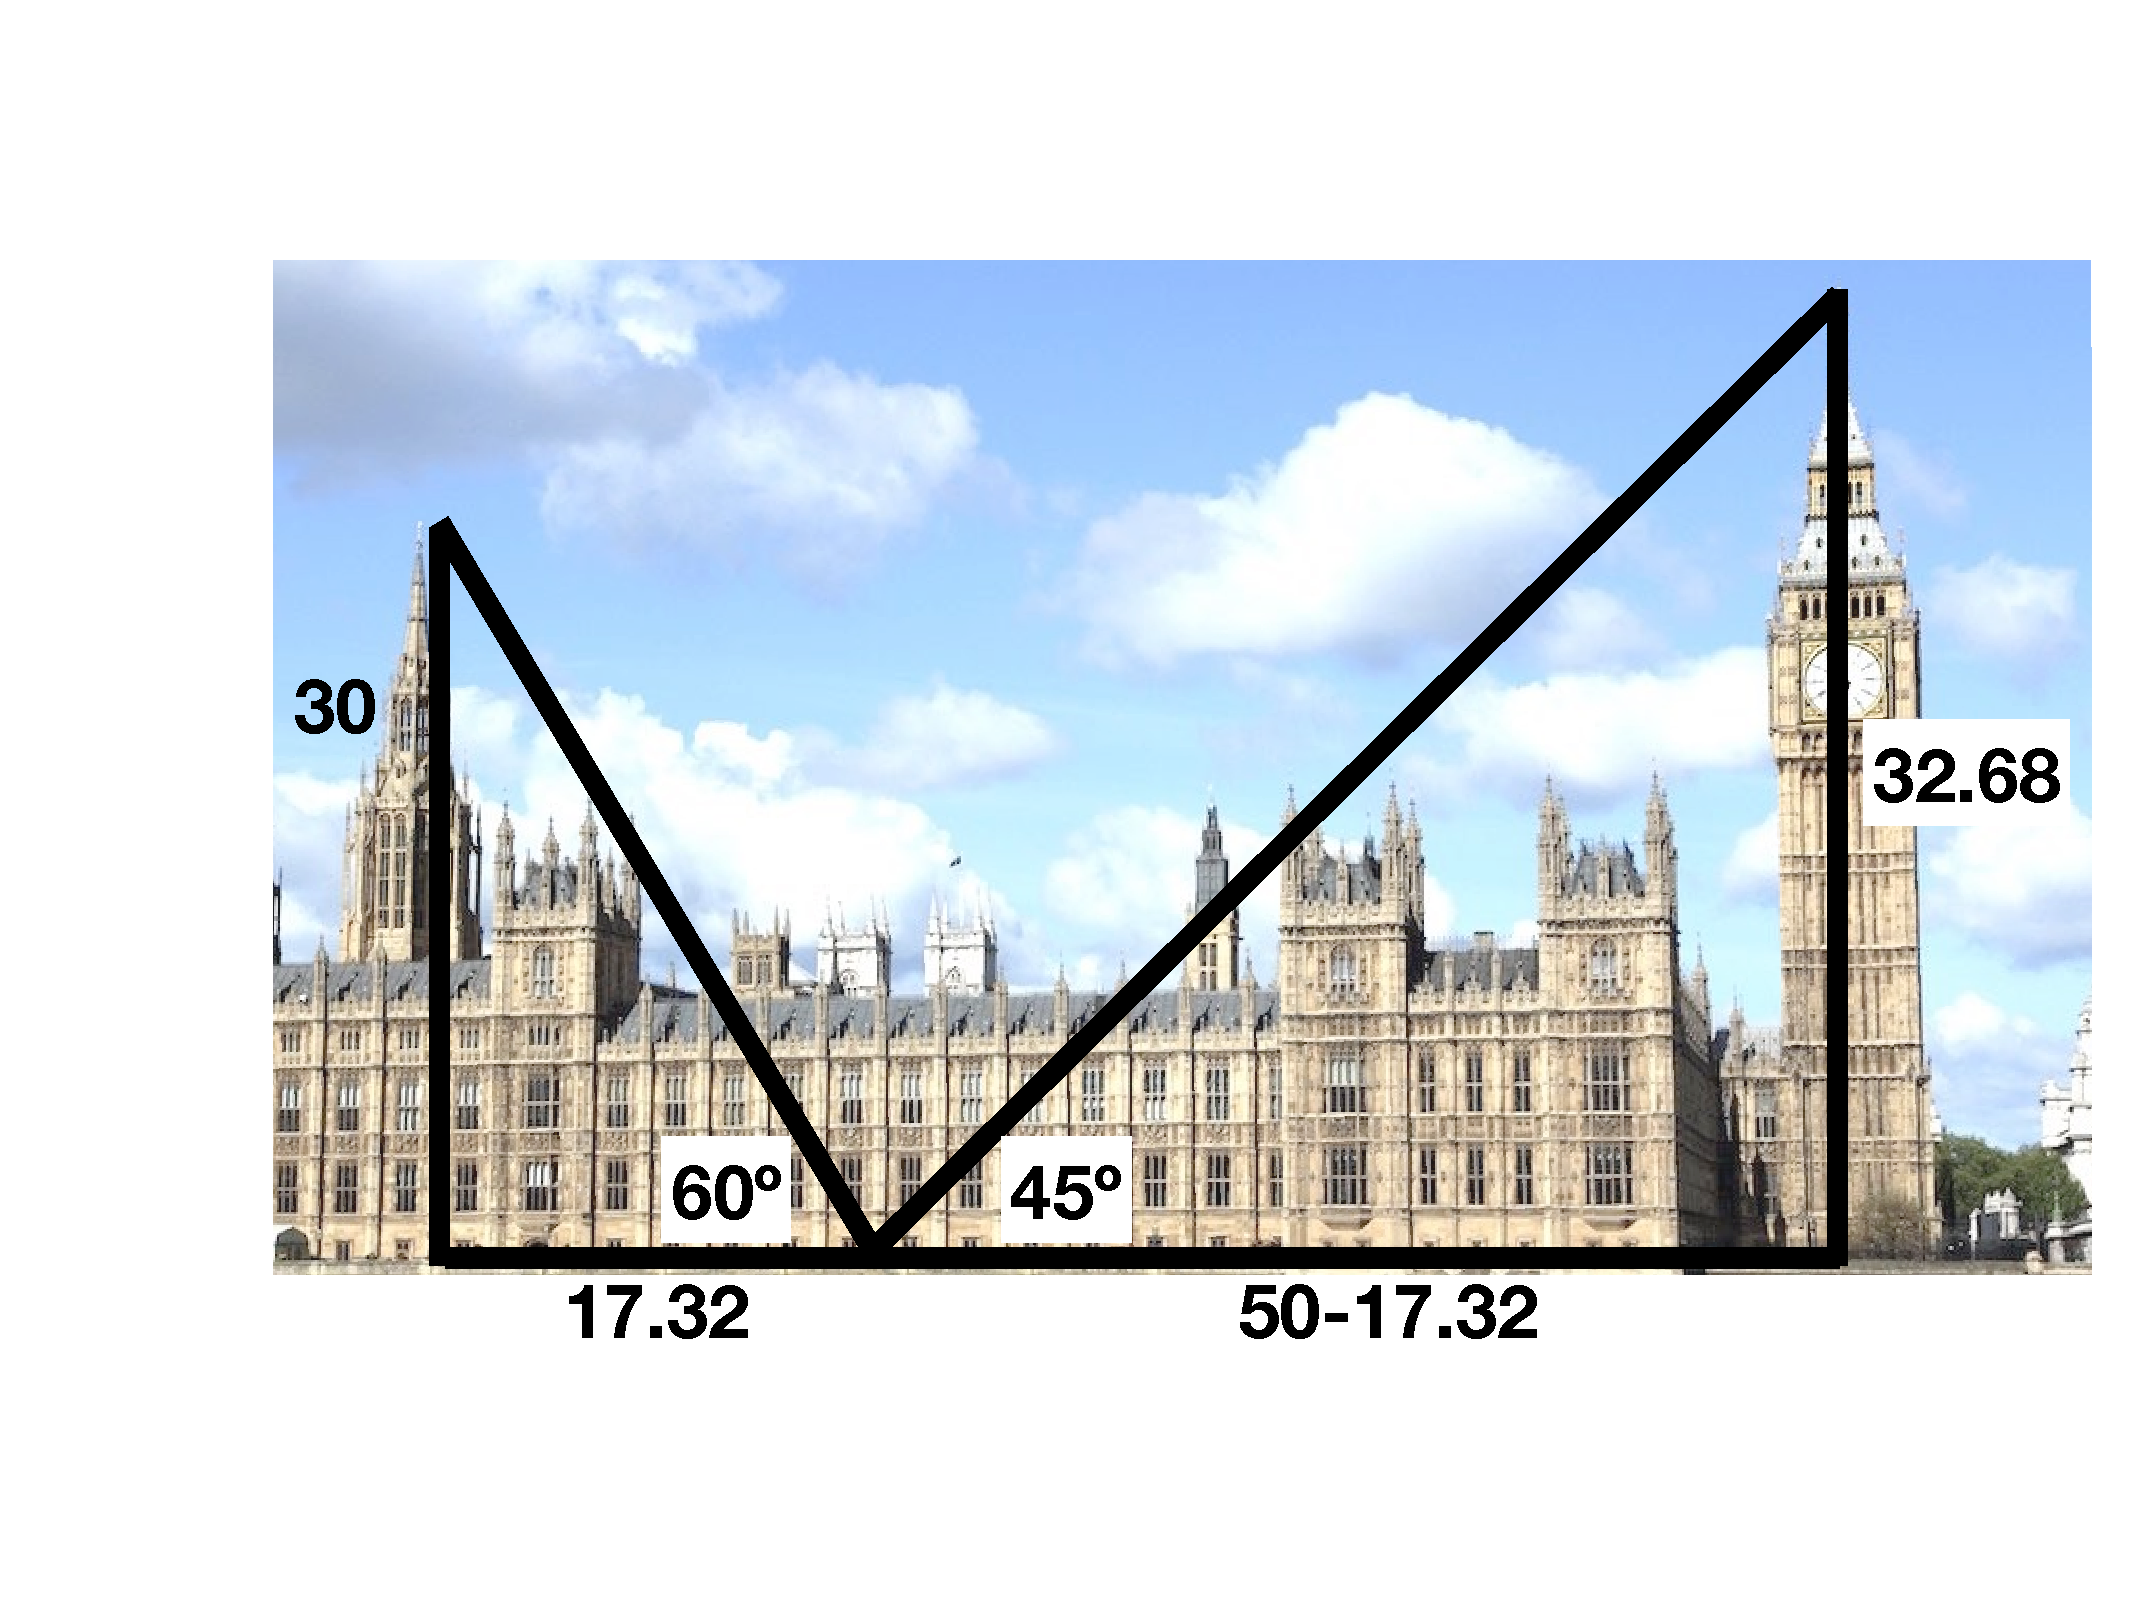
\includegraphics[width=0.4\textwidth]{img-sol/t3-47}}
\end{mylist}

\section{Identitats trigonomètriques}

\begin{theorybox}{Trobareu un resum de les identitats trigonomètriques a la pàgina \pageref{sec:formularitrig}.}
	\vspace{0.4cm}
	
	\begin{minipage}{0.25\textwidth}	
		\centering
		\videonw{145}{Identitats  1: Suma d'angles}
		
	\end{minipage}
	\begin{minipage}{0.25\textwidth}
		\centering
		\videonw{146}{Identitats  2: Diferència d'angles}
		
	\end{minipage}
	\begin{minipage}{0.25\textwidth}
		\centering
		\videonw{148}{Identitats  3: Angle doble}
		
	\end{minipage}
	\begin{minipage}{0.25\textwidth}
		\centering
		\videonw{147}{Identitats  4: Relació de l'angle meitat}
		
	\end{minipage}
	
	\vspace{0.5cm}
\end{theorybox}

\begin{mylist}
	\exer
	Calcula a partir de les raons trigonomètriques de
	30${}^\circ$, 45${}^\circ$, 60${}^\circ$ i
	90${}^\circ$, les raons trigonomètriques de
	75${}^\circ$, 120${}^\circ$, 150${}^\circ$, 
	105${}^\circ$ i 135${}^\circ$
	
	\begin{example}[*]
		Per exemple, si utilitzam la relació de la suma d'angles i expressam $75^\circ =45^\circ + 30^\circ$
		
		$\sin(75^\circ)=\sin(45^\circ + 30^\circ)=\sin(45^\circ)\cdot \cos(30^\circ) + \cos(45^\circ)\cdot \sin(30^\circ)=\frac{\sqrt{2}}{2}\frac{\sqrt{3}}{2}+\frac{\sqrt{2}}{2}\frac{\sqrt{1}}{2}=\frac{\sqrt{6}+\sqrt{2}}{4}$
	\end{example}
	
	\begin{example}[*]	
		De forma similar, podem obtenir el cosinus
		
		$\cos(75^\circ)=\cos(45^\circ + 30^\circ)=\cos(45^\circ)\cdot \cos(30^\circ) - \sin(45^\circ)\cdot \sin(30^\circ)=\frac{\sqrt{2}}{2}\frac{\sqrt{3}}{2}-\frac{\sqrt{2}}{2}\frac{\sqrt{1}}{2}=\frac{\sqrt{6}-\sqrt{2}}{4}$
		
		i finalment, la tangent
		
		$\tg(75^\circ)=\tg(45^\circ + 30^\circ)=\dfrac{\tg 45^\circ + \tg 30^\circ}{1-\tg 45^\circ \cdot \tg 30^\circ}=\dfrac{1 + \frac{\sqrt{3}}{3}}{1-1 \cdot \frac{\sqrt{3}}{3}}=2+\sqrt{3}$
	\end{example}
	
	\exer
	Calcula a partir de les raons trigonomètriques de
	30${}^\circ$, 45${}^\circ$, 60${}^\circ$ i
	90${}^\circ$, les raons trigonomètriques de
	15${}^\circ$
	
	\answers{15=45-30; $\sin 15=\sin 45\cos 30 - \cos 45 \sin 30= \dfrac{\sqrt{6}-\sqrt{2}}{4}$ \par $\cos 15=\cos 45\cos 30 + \sin 43 \sin 30= \dfrac{\sqrt{6}+\sqrt{2}}{4}$ \par $\tg 15=2-\sqrt{3}$ }
	
	\exer
	Comprova que les raons trigonomètriques de 30${}^\circ$ es
	poden obtenir a partir de les raons trigonomètriques de 90${}^\circ$, 
	i de 60${}^\circ$.
	
	\answers{30=90-60; $\sin 30=\sin 90\cos 60 - \cos 90 \sin 60= \cos 60 = \dfrac{1}{2}$ \par $\cos 30=\cos 90\cos 60 + \sin 90 \sin 60= \sin 60 =\dfrac{\sqrt{3}}{2}$ \par $\tg 60=\sqrt{3}$ }
	
	
	\exer
	Demostra les fórmules d'angles complementaris ($90-\alpha$) emprant les fórmules de la
	diferència: $\sin(90-\alpha)=\cos\alpha$, $\cos(90-\alpha)=\sin\alpha$ i $\tg(90-\alpha)=1/\tg\alpha$.
	
	\answers{$\sin(90-\alpha)=\sin 90 \cos \alpha - \cos 90 \sin \alpha = \cos \alpha$,\par $\cos(90-\alpha)=\cos 90 \cos \alpha + \sin 90 \sin \alpha=\sin\alpha$ i $\tg(90-\alpha)= 1/\tg\alpha$}
	
	\exer
	Calcula les raons trigonomètriques de
	22'5${}^\circ$ i 11'25${}^\circ$ a partir de les
	raons trigonomètriques de 45${}^\circ$.
		
	\answers{$22.5 = 45/2$, $\sin 22.5= \dfrac{\sqrt{2-\sqrt{2}}}{2}$, $\cos 22.5= \dfrac{\sqrt{2+\sqrt{2}}}{2}$, $\tg 22.5= \sqrt{3-2\sqrt{2}}$\par
		$11.25 = 22.5/2$, $\sin 11.25= \frac{\sqrt{2-\sqrt{2+\sqrt{2}}}}{2}$, $\cos 11.25= \frac{\sqrt{2+\sqrt{2+\sqrt{2}}}}{2}$, $\tg 11.25= -1-\sqrt{2}+\sqrt{2(2+\sqrt{2})}$
	}
	
	
	
	\exer
	Comprova que les raons trigonomètriques de 45${}^\circ$ es
	poden obtenir a partir de les raons trigonomètriques de 90${}^\circ$.
	\answers{$45 = 90/2$, $\sin 45= \sqrt{\frac{1-\cos 90}{2}}=\frac{\sqrt{2}}{2}$, $\cos 45= \sqrt{\frac{1+\cos 90}{2}}=\dfrac{\sqrt{2}}{2}$,\par $\tg 45= \sqrt{\dfrac{1-\cos 90}{1+\cos 90}}=1$}
	
	
	\exer[-1] Demostra $\sin^2 \alf \cdot \cos \alf + \cos^3 \alf= \cos \alf$. 
	\answers{Treu factor comú $\cos \alpha$ i utilitza la relació fonamental.}
	
	\end{mylist}
	
	\begin{example}
		Per fer una demostració d'una identitat cal partir del terme de l'esquerre i, aplicant altres relacions que sabem que són certes, arribar al terme de la dreta que volem demostrar. 
		
		Així doncs, en aquest exemple partirem de $\sin^2 \alf \cdot \cos \alf + \cos^3 \alf$ i treurem factor comú $\cos \alf$, obtenint
		
		$\sin^2 \alf \cdot \cos \alf + \cos^3 \alf = \cos\alf \cdot (\sin^2 \alf + \cos^2 \alf)$ ara utilitzam la relació fonamental que diu que $\sin^2 \alf + \cos^2 \alf=1$, aleshores trobam $\sin^2 \alf \cdot \cos \alf + \cos^3 \alf = \cos\alf$ que era el resultat que voliem demostrar (\textbf{c.v.d.}).
		
	\end{example}
	
	
	\begin{mylist}
		
	\exer[-1] Demostra $(\sin \alf + \cos \alf)^2 = 1 + \sin 2\alf$. 
	\answers{Desenvolupa el quadrat amb la identitat notable $(a+b)^2 = a^2 + b^2 + 2ab$. Empra la relació fonamental i la fórmula de $\sin 2\alf$.}
	
	\exer[-1] Demostra $2\sin x + \cos(-x)-\sin(-x)-\cos x = 3 \sin x$. 
	\answers{Utilitza les relacions de l'angle oposat $\cos(-x)=\cos x$, $\sin(-x)=-\sin x$, $\tg(-x)=-\tg x$.}
	
	\exer[-1] Demostra $\tg \alf + \cotg \alf = \sec \alf \cdot \cosec \alf$. 
	\answers{Expressa $\tg \alf$ i $\cotg \alf$ com a quocients de sinus i cosinus. Després realitza la suma de fraccions amb el
	mínim comú múltiple. Finalment utilitza la relació fonamental.}
	
	\exer[-1] Demostra $\sin 3\alf = \sin\alf \cdot \left( 3\cos^2 \alf - \sin^2 \alf \right)$. 
	\answers{Escriu $\sin(3\alf) = \sin(\alf+2\alf)$. Aplica la fórmula de la suma d'angles i tot seguit les
	fórmules de l'angle doble. Finalment opera, simplifica i treu factor comú $\sin \alf$.}
	
	\exer[-1] Demostra $\cos 4\alf = \cos^4\alf+\sin^4\alf-6\sin^2 \alf \cos^2 \alf$. 
	\answers{Escriu $\cos(4\alf) = \cos(2\alf+2\alf)$. Aplica la fórmula de la suma d'angles i tot seguit les
	fórmules de l'angle doble. Finalment opera i simplifica.}
	
	
	\exer Simplifica les següents expressions:
	\begin{tasks}(2)
		\task $(\sin x + \cos x)^2 + (\sin x - \cos x)^2$
		\task $\dfrac{\sin(2 a)\cdot \cos a}{\sin a \cdot (1+\cos(2 a))}$
		\task $\dfrac{\sin^3 x+\sin x \cdot \cos^2 x}{\sin x}$
		\task $\dfrac{\sin(x-y)-\sin(x+y)}{\cos(x+y)-\cos(x-y)}$
	\end{tasks}
\answers{[2, 1, 1, $\cotg x$]}
	
	
%	\exer
%	Comprova si són certes o falses les següents igualtats: 
%	\begin{tasks}(2)
%		\task $\dfrac{1+\tg^{2} x}{1+\cotg^{2} x} =\tg^{2} x$
%		\task $\dfrac{\sin\left(2x\right)}{1+\cos \left(2x\right)} =\tg x$
%	\end{tasks}


	\exer
	Demostra que són certes les següents igualtats: 
	\begin{tasks}(2)
		\task $\dfrac{2\sin x}{\tg 2x} =\cos x-\dfrac{\sin^{2} x}{\cos x} $
		\task $\dfrac{1-\sin^{4} x}{\cos ^{2} x} =2-\cos ^{2} x$
	\end{tasks}
	\exer
	Comprova que són certes les següents igualtats: 
	\begin{tasks}(2)
		\task $\dfrac{1+\tg^{2} \alpha }{1+\cotg^{2} \alpha } =\tg^{2} \alpha $
		\task $\dfrac{\cos ^{2} \alpha }{1+\sin\alpha } =1-\sin\alpha $
	\end{tasks}
	
	\exer
	Utilitza les transformacions de sumes en productes per posar en funció
	del sinus i cosinus de l'angle $a$:
	
	\begin{tasks}(2)
		\task $\sin(45+a) + \sin(45 -a)$
		\task $\cos(120+a) + \cos(60 + a)$
	%	\task $\cos(270- a ) - \cos(90 - a)$
	\end{tasks}

\answers{[$\sqrt{2}\sin a$, $-\sqrt{3}\sin a$]}
	
	
	\exer
	Demostra les següents identitats:
	\begin{tasks}(2)
		\task $\tg x \cdot \cos x = \sin x$
		\task $1+\tg^2 x = \sec^2 x$
		\task $1+\cos 2x = \dfrac{2}{1+\tg^2 x}$
		\task $\dfrac{\cos x + \sin x}{\cos x - \sin x}\cdot \cos 2x = 1 + \sin 2x$
	\end{tasks}
	
\end{mylist}



\section{Equacions i sistemes trigonomètrics}

 \begin{warningbox}
	\begin{multicols}{2}
		
		\heading{Identitat}:  $\mathbf{(x+1)^2=x^2+2x+1}$
		
		{\footnotesize És certa sempre, per qualsevol $x$}
		
		\columnbreak
		
		\heading{Equació}: $\mathbf{x^2 -x =2}$
		
		{\footnotesize Volem trobar els valors de $x$ pels quals es compleix $=$}
	\end{multicols}
\end{warningbox}

\begin{theorybox}
	\begin{minipage}{0.33\textwidth}
		\centering
		\videonw{138}{Equacions trigonomètriques nivell 1}
	\end{minipage}
	\begin{minipage}{0.33\textwidth}
		\centering
		\videonw{139}{Equacions trigonomètriques nivell 2}
	\end{minipage}
	\begin{minipage}{0.33\textwidth}
		\centering
		\videonw{140}{Equacions trigonomètriques nivell 3}
	\end{minipage}
\end{theorybox}

\begin{mylist}
	\exer
	Resol les següents equacions trigonomètriques
	\begin{tasks}(3)
		\task $\cos x = -\frac{1}{2}$
		\task $\tg x = \sqrt{3}$
		\task $\sin x = -\frac{\sqrt{2}}{2}$
%%
		\task $\tg x = -1$
		\task $\cosec x = 4$
		\task $\cos x = \frac{1}{3}$
%%
		\task $\sin x = \cos x$
		\task $\tg^2 x = \frac{1}{3}$
		\task $\cos^2 x = \frac{1}{2}$
	\end{tasks}
\answers[cols=1]{[$x=120+n\cdot 360$ i $x=240+n\cdot 360$, 
				  $x=60+n 180$,  
				  $x=225+n\cdot 360$ i $x=315+n\cdot 360$, 
				  $x=135+n\cdot 360$, 
				  $x=14.48 + n \cdot 360$ i $x=165.52 + n \cdot 360$,
				  $x=70.53 + n \cdot 360$ i $x=289.47 + n \cdot 360$, 
				  $x=45 + n \cdot 360$, 
				  $x=30,\;150,\;210,\;330 + n \cdot 360$, 
				  $x=45,\;135,\;225,\;315 + n \cdot 360$]}
 
	
	\exer
	Calcula les solucions de les següents equacions trigonomètriques
	\begin{tasks}(3)
		\task $\cos(3 x) = 0$
		\task $\tg(2 x) = -1$
		\task $\sin(4 x) = -1$
	\end{tasks}
	Expressa en radiants les solucions anteriors.
 
 \answers[cols=1]{[$x=30+n\cdot 60$, $x=67.5+n\cdot 90$, $x=67.5+n\cdot 90$]}
	
	\exer
	Calcula les solucions de les següents equacions trigonomètriques:
	\begin{tasks}(2)
		\task $\cos(5 x) - \cos x = 0$
		\task $\sin(2 x) - \sin(4 x) = 0$
	\end{tasks}
	\textit{Ajuda:} Utilitza les relacions:\par \qquad $\cos a - \cos b =-2\sin \frac{a+b}{2} \sin \frac{a-b}{2}$ \quad i \quad $\sin a - \sin b =2\cos \frac{a+b}{2} \sin \frac{a-b}{2}$.
	
	\answers[cols=1]{[$x=n\cdot 60$ i $x=n\cdot 90$, $x=30+n\cdot 60$ i $x=n\cdot 180$]}
	
	\exer
	Calcula les solucions de les següents equacions trigonomètriques:
	\begin{tasks}(2)
		\task $\sin x + \cos x = 1$
		\task $\sin (2 x) = 2 \cos x$
		\task $\sin^2 x - \cos^2 x - \cos(2 x)=1$
	\end{tasks}
\answers[cols=1]{[Elevau al quadrat i comprovau les solucions: 
$x=90+n\cdot 360$ i $x=n\cdot 360$, $x=90+n\cdot 180$, $x=60+n\cdot 180$  i $x=120+n\cdot 180$]}
	
\end{mylist}

\begin{mylist}
	
	
	\exer  Resol les següents equacions trigonomètriques: 
	\begin{tasks}(2)
		\task $\cos x\cdot \cos 2x+2\cos ^{2} x=0$ 
		\task   $\tg x-\sin 2x=0$
	\end{tasks}
	\answers[cols=1]{[$x=90+n\cdot 180$ i $x=68.53+n\cdot 360$ i $x=291.47+n\cdot 360$,  $x=n \cdot 180$ i $x=45+n\cdot 90$]}

	
	\exer  Resol les equacions trigonomètriques següents donant totes les solucions possibles.
	\begin{tasks}(2)
		\task  $\cos 2x+1=4\cos x $  
		\task  $\dfrac{\sin\left(2x\right)}{\tg x} +\cos ^{2} x=1$ 
		\task  $\cos 2x+\cos x=0,2$
	\end{tasks}
	
	\answers[cols=1]{[Anomenam $c=\cos x$. Només si $c=0$; dóna $x=90+n\cdot 180$, Només si $c=\pm 1/\sqrt{3}$; dóna $x=54.73+n\cdot 180$ i $x=125.27+n\cdot 180$,  Només prové solució de $c=0.5639$; dóna $x=55.67+n\cdot 360$ i $x=304.33+n\cdot 360$]}
	
	\exer  Resol les següents equacions 
	\begin{tasks}(2)
		\task $\sin^2 x - \sin x = 0$
		\task $\cos x + \sin^2 x = 1$
		\task $3\tg^2 x = \sec^2 x$
		\task $\sin 2x = 0,5$  
	\end{tasks}
	\answers[cols=1]{[$x=n\cdot 180$ i $x=90+n\cdot 360$, $x=90+n\cdot 180$ i $x=n\cdot 360$, $x=35.26+n\cdot 180$ i $x=144.74+n\cdot 180$, $x=15+n\cdot 180$ i $x=75+n\cdot 180$]}
	
	\exer
	Resol els següents sistemes:
	\begin{tasks}(2)
		\task 
		$\left\{ \begin{array}{l}  
		x+ \sin^2 y =2 \\ 
		x+\cos^2 y =1
		\end{array}  \right.$
		\task 	 
		$\left\{ \begin{array}{l}  
		\sin x \cdot \cos y = \frac{3}{4} \\ [0.2cm]
		\cos x \cdot \sin y = \frac{1}{4}
		\end{array}  \right.$
	\end{tasks}
\answers[cols=1]{[Sumar les dues equacions i aplica identitat fonamental $x=1;\,y=90+n\cdot 180$, Suma les dues i aplica sinus d'una suma. Fes el mateix restant-les\par Arribes al sistema $\left\{\begin{array}{l}
	\sin(x+y)=1 \\ \sin(x-y)=1/2
	\end{array} \right.$.\par Trobam $x=60+n\cdot 180;\,y=30+n'\cdot 180$ i $x=120+n\cdot 180;\,y=150+n'\cdot 180$ ]}
	
	\exer  Resol els següents sistemes: 
	\begin{tasks}(2)
		\task 
		$\left\{ \begin{array}{l}  
		\sin x - \sin y = 0 \\ 
		x - y = \pi
		\end{array}  \right.$
		\task 	 
		$\left\{ \begin{array}{l}  
		\sin x \cdot \cos y = \frac{1}{2} \\  
		x + y = \frac{\pi}{2}
		\end{array}  \right.$
	\end{tasks}

\answers[cols=1]{[Substitució $x=n\pi;\,y=(n-1)\pi$, $x=\frac{\pi}{4}+n\frac{\pi}{2};\,y=\frac{\pi}{4}-n\frac{\pi}{2}$]}


 
	\exer Resol els següents sistemes:  
	\begin{tasks}(2)
		\task 
		$\left\{ \begin{array}{l}  
		\cos(x-y)=0\\ 
		\cos(x+y)=0
		\end{array}  \right.$
		\task 	 
		$\left\{ \begin{array}{l}  
		\sin(x-y)=\frac{1}{2}\\[0.2cm]
		\cos(x-y)=\frac{1}{2}  
		
		\end{array}  \right.$
	\end{tasks}
 
 \answers[cols=1]{[$x=90+(n+m)\cdot 90; y=(m-n)\cdot 90$, per a tot $n$ i $m$ enter., No té solució  perquè si elevam al quadrat i sumam $\sin^2 (x-y)+\cos^2 (x-y)=\frac{1}{2}$, quan la relació fonamental requereix que $\sin^2 \alpha +\cos^2 \alpha=1$]}
 
\end{mylist}




 
\newpage
\begin{autoaval}{50}

\begin{mylist}

\exer[2]
  Calcula les següents raons trigonomètriques sense fer ús de la
  calculadora.
  \begin{tasks}(3)
    \task $\sin (-750^\circ)$
    \task $\tg 570^\circ$ 
    \task $\cos (2\pi/3)$
  \end{tasks}
\answers[cols=1]{[$\sin(-750^\circ)=1/2$, $\tg 570^\circ=\frac{-1}{\sqrt 3}=-\frac{\sqrt 3}{3}$,  $\cos 20\pi/3 = -1/2$]}


\exer[2]
  A partir de les raons trigonomètriques de la suma d'angles, calcula exactament les següents
  raons trigonomètriques:

  \begin{tasks}(2)
 	\task $\sin 105^\circ$
    \task $\cos 75^\circ$
  \end{tasks}
\answers{$\sin(105)=\sin(60+45)=\frac{\sqrt{6}+\sqrt{2}}{4}$ \par
	$\cos(75)=\sin(30+45)=\frac{\sqrt{6}-\sqrt{2}}{4}$}

\exer[2]
  Sigui un triangle del que coneixem les següents dades \emph{a =} 10
  cm, \emph{b} = 20 cm, = 30${}^\circ$\textbf{.} Calcula les altres dades del
  triangle. Calcula l'àrea del triangle
\answers{$c=17,32$, $\hat B=90^\circ$, $\hat C=60^\circ$}

\exer[2]
  Un voltor vola a 120 m d'altura i formant un angle amb l'horitzontal
  respecte de nosaltres de 60${}^\circ$. En la mateixa direcció
  però formant un angle de 30 ${}^\circ$ vola una perdiu a 100
  m d'altura. Si el voltor vol menjar-se la perdiu, però només ho
  aconsegueix si la distància entre tots dos és menor de 150 m, pot el
  voltor caçar a la perdiu? A quina distància estan?
\answers{Sí ho aconseguirà. Estan a 105,83 m.}

\exer[2]
  Calcula sense utilitzar la calculadora la resta de raons
  trigonomètriques (sinus, cosinus) de $\alpha$ , sabent que  $\tg \alpha = 1/2$ i
  $\alpha$ pertany al 3r quadrant.
\answers{$\sin a=\frac{-1}{\sqrt 5}=-\frac{\sqrt 5}{5}$\par
	$\cos a=\frac{-2}{\sqrt 5}=-\frac{2\sqrt 5}{5}$;}

\exer[2]
  Resol les següents equacions: 
  \begin{tasks}(2)
  \task $6 \cos^2 (x/2) + \cos x=1$
  
  \task $\sin x + \cos x = \sqrt{2}$
  \end{tasks}
\answers{a) $x=\left\{\begin{array}{l} 120 + n 360 \\ 240 +n 360 \end{array}\right.$  \par b) $x=45 + n 180$}

\exer[2]
  Resol els següents sistemes: 
  \begin{tasks}(2)
  \task $\left\{ \begin{array}{ll} \sin x + \sin y &=1 \\ x+y&=\pi \end{array} \right.$
  
  \task $\left\{ \begin{array}{ll} \sin x + \sin y&= \frac{\sqrt{3}+1}{2} \\\sin x - \sin y &= \frac{\sqrt{3}-1}{2} \end{array} \right.$
\end{tasks}
\answers{a) $(60+360k,120–360k)$ i \par $(120+360k,60–360k)$; \par
	b) $(75+360k, 15–360k)$ i \par $(15+360k, 75–360k)$}
 

\exer[2]
  Demostra la identitat
 $\dfrac{\sin^2 2a}{(1-\cos^2 a) \cdot \cos a}=4 \cos a$
\answers{Substituir el $\sin(2a)$ pel seu valor i aplicar  que $1–\cos 2a$ és el sinus al quadrat.}


\exer[2]
  Calcula el perímetre d'un pentàgon regular inscrit en una
  circumferència de 30 cm de radi. Calcula la seva àrea
\answers{Perímetre = $5 \cdot 35.267 = 176,3355$ m; Apotema $a_p =  30 \cos 36 =24.27$; \quad Àrea = 2139.83 m$^2$.}

\exer[2]
  En els senyals de trànsit que indiquen el pendent de la carretera la
  informació que ens donen és el percentatge de pujada en funció de
  l'avanç del cotxe. Calcula l'angle per a un pendent del 15 \%.
\answers{$8,63^\circ$}

\end{mylist}
\end{autoaval}

\newpage
\heading{Aplica el que has après}

\subsection*{Una barrera conflictiva}

Un dia que anava passejant em vaig trobar la barrera de la imatge. Sembla com si el ferrer hagués tingut alguns problemes a l'hora de construir-la. Com pots veure, va començar amb cercles i al final va intentar acabar-la amb alguna cosa semblant a el·lipses. Això passa, perquè el ferrer va col·locar les divisions verticals a igual distància.

\includegraphics*[width=0.5\textwidth]{img-03/barrera}
\includegraphics*[width=0.5\textwidth]{img-03/chap-trig-barrera-scheme}

Em demano com hauria d'haver estat el disseny perquè es pogués fer únicament amb cercles tangents entre sí i tangents amb les barres horitzontals (vegeu esquema de la dreta). En particular, quina hauria d'ésser la relació entre els radis de dos cercles consecutius $\frac{r}{R}$ sabent que les dues barres horitzontals formen un angle $\alpha$?

\subsection*{Encerclant l'euro}

\begin{minipage}{0.7\textwidth}
No us ha passat mai que estau avorrits i començau a jugar amb el primer que teniu a ma? Un dia tenia moltes monedes dins la butxaca i vaig començar a encerclar 1 € amb monedes de cèntim. Em demanava si era possible trobar alguna combinació de monedes de forma que la corona de monedes es pugues fer de la forma més exacta possible; és a dir, que totes les monedes fossin tangents entre si.
\end{minipage}
\begin{minipage}{0.3\textwidth}
 \includegraphics*[width=0.75\textwidth]{img-03/monedes}
\end{minipage}

Potser et sigui d'utilitat disposar dels radis de les monedes d'euro:
\begin{center}
\begin{tabular}{|c|c|c|c|c|c|c|c|c|c|}
	\hline 
	Moneda & 0.01 €  & 0.02 € & 0.05 € & 0.10 € & 0.20 € & 0.50 € & 1 € & 2 €\\ 
	\hline 
	Diametre (mm) & 16.25  & 18.75  & 21.25 & 19.75 & 22.25 & 24.25  & 23.25 & 25.75 \\ 
	\hline 
\end{tabular}
\end{center} 


\begin{minipage}{0.65\textwidth}
	Començau l'anàlisi a partir de l'esquema de la dreta. Si es possible enrevoltar el cercle gran amb els petits, voldrà dir que l'angle $\alpha$ serà una part de $360^\circ$; és a dir,  $\alpha=360 / n$ per algun $n=3,4,5,\cdots$. A partir de trigonometria en un dels triangles, trobau una relació entre els radis de les monedes $R/r$ perquè l'encerclament sigui perfecte. 
\end{minipage}
\begin{minipage}{0.35\textwidth}
	\includegraphics*[width=\textwidth]{img-03/chap-trig-monedes-scheme}
\end{minipage}

\newpage
 
\resum

\begin{center}
	\setlength\LTleft{0pt}
	\setlength\LTright{0pt}
	\ftimes{10.5}{11}
	\fontsize{10.5}{11}
	\renewcommand{\arraystretch}{2}
	\begin{longtable}[h]{|>{\raggedleft\arraybackslash}p{0.19\linewidth}|p{0.77\linewidth}|}
		\toprule %inserts double horizontal lines
		\rowcolor{lightgray}
		
		\textbf{Apartat} & \textbf{Resum} \\   [0.5ex] 
		\toprule  \hline
		
		
		\cellcolor{lightgray}\noindent \textbf{Radiant}  &   
		És un angle tal que qualsevol arc que se li associï mesura exactament el mateix que el radi utilitzat per traçar-ho. Es denota per \textit{rad}.  $360^\circ = 2\pi$ rad
		\sample{
		$180^\circ$ són $\pi$ rad, $90^\circ$ són $\pi/2$ rad, ...
		}
		\hline

\cellcolor{lightgray}\noindent \textbf{Raons d'un angle agut}  &  

\begin{minipage}{0.4\textwidth}
	$\sin\; \alpha \; =\; \; \frac{\text{catet oposat}}{\text{hipotenusa}} \; \; =\; \; \frac{b}{a} $\newline $\cos \; \alpha \; \; =\; \; \frac{\text{catet contigu}}{\text{hipotenusa}} \; \; =\; \; \frac{c}{a} $\newline $\tg\alpha \; \; =\; \; \frac{\text{catet oposat}}{\text{catet   contigu}} \; \; =\; \; \frac{b}{c} $
\end{minipage}
\begin{minipage}{0.3\textwidth}
	\includegraphics*[width=1.18in, height=0.92in, keepaspectratio=false]{img-03/image495.png}
	 
		$\sin \beta=\frac{3}{5} $, $\cos \beta=\frac{4}{5}$, $\tg \beta = \frac{3}{4} $ 
\end{minipage} 
\\
\hline

\cellcolor{lightgray}\noindent \textbf{Teorema del sinus}  &   
En un triangle $\widehat{\mathop{ABC}}$ qualsevol:    
	\begin{eqnarray*}
	\frac{a}{\sin \hat A}=\frac{b}{\sin \hat B}=\frac{c}{\sin \hat C}=2R
\end{eqnarray*}
on $R$ és el radi de la circumferència circumscrita en el triangle.
\sample{
	Si $b=5$ i $a=3,01$ i  $\hat B=30^\circ$, l'angle $\hat A$ compleix  $	\frac{3,01}{\sin \hat A}=\frac{5}{\sin \hat 30}$  i dóna $\hat A =17\, '\, 52^\circ$
}
\hline

\cellcolor{lightgray}\noindent \textbf{Teorema del cosinus}  &   
En un triangle\textit{ ABC} qualsevol: 

\[a^{2} =b^{2} +c^{2} -2bc\cos \hat A \]
\[b^{2} =a^{2} +c^{2} -2ac\cos \hat B \]
\[c^{2} =a^{2} +b^{2} -2ab\cos \hat C \]
\sample{
	Si \textit{b} = 5, \textit{c} = 6 i l'angle entre ells és 30 graus, el costat \textit{a} és\newline $a^{2} =5^{2} +6^{2} -60\cos 30$= 9,04  $\rightarrow$  $a=3,01$
}
\hline

\cellcolor{lightgray}\noindent \textbf{Resolució general de triangles}  &   
En general, qualsevol triangle es pot resoldre si coneixem tres de les sis dades (hi ha tres costats i tres angles). Almenys necessitam conéixer un costat.\newline S'apliquen els teoremes del sinus i del cosinus i que la suma dels seus angles són 180 graus.  
\sample{
	Si les dades originals són \textit{b}=5, \textit{c} = 6 i $\hat A =30$ el teorema del cosinus ens dóna  a = 3'01, el teorema del sinus $\hat A =17\, '52^\circ$ i $\hat B =132'48^\circ$.
}
\hline \bottomrule
	\end{longtable}
\end{center}

\pagebreak
 

\heading{Resum d'identitats trigonomètriques}
\label{sec:formularitrig}
\begin{bluebox}
 \textbf{Relacions fonamentals:}
 
\quad [1]\; $\sin^2 \alpha + \cos^2 \alpha = 1$ \qquad     
[2]\; $\tg \alpha = \dfrac{\sin \alpha}{\cos \alpha}$ \qquad   
[3]\; $1 + \tg^2 \alpha = \dfrac{1}{cos^2 \alpha}$    

 
 \textbf{Angle oposat:}
 
 \quad [4]\; $\sin(-\alpha)=-\sin \alpha$,  \quad$\cos(-\alpha)= \cos \alpha$, \quad $\tg(-\alpha)=-\tg \alpha$

 \textbf{Suma d'angles:}
 
\quad  [5]\; $     \sin (\alpha+\beta)=\sin \alpha\, \cdot \, \cos \beta+\cos \alpha\, \cdot \, \sin \beta$ 
 
 \quad [6]\; $     \cos (\alpha+\beta)=\cos \alpha\, \cdot \, \cos \beta-\sin \alpha\, \cdot \, \sin \beta$ 
 
 \quad [7]\;$     tg(\alpha+\beta)=\dfrac{tg\, \alpha+tg\, \beta}{1-tg\, \alpha\; \cdot \; tg\, \beta} $ 
 

 
 \textbf{Diferència d'angles:}
 
 \quad [8]\; $  \sin (\alpha-\beta)=\sin \alpha\, \cdot \, \cos \beta-\cos \alpha\, \cdot \, \sin \beta$ 
 
 \quad [9]\;  $ \cos (\alpha-\beta)=\cos \alpha\, \cdot \, \cos \beta+\sin \alpha\, \cdot \, \sin \beta$ 
 
 \quad  [10]\; $ tg(\alpha-\beta)=\dfrac{tg\, \alpha - tg\, \beta}{1+tg\, \alpha\; \cdot \; tg\, \beta} $ 
 \textbf{}
 
  
 \textbf{Angle doble:}
 
 \quad  [11]\; $  \sin 2\alpha=2\sin \alpha\, \cdot \, \cos \alpha$ 
 
 \quad [12]\; $  \cos 2\alpha=\cos ^{2} \alpha-\sin ^{2} \alpha$ 
 $=2\cos^2 \alpha-1$ 
 $=1-2 \sin^2 \alpha$ 
 
 \quad [13]\; $  tg\, 2\alpha=\dfrac{2\, tg\, \alpha}{1-tg^{2} \alpha} $ 
 \textbf{}
 
 
 
 \textbf{Angle meitat:}
 
 \begin{minipage}{0.5\textwidth}
 
 \quad [14]\; $  \sin \frac{\alpha}{2} =\pm \sqrt{\dfrac{1-\cos \alpha}{2} } $ 
 
 \quad [15]\; $  \cos \frac{\alpha}{2} =\pm \sqrt{\dfrac{1+\cos \alpha}{2} } $ 
 
 \quad [16]\; $   \tg\frac{\alpha}{2} =\pm \sqrt{\dfrac{1-\cos \alpha}{1+\cos \alpha} } $ 
 
 \end{minipage}
\begin{minipage}{0.4\textwidth}
$\mathrm{signe\ \pm segons\ quadrant\ de\ } \alpha/2$ 
\end{minipage}

 
 
 
 
 \textbf{Sumes i diferències a  productes:}
 
 \quad [17]\; $  \sin \alpha+\sin \beta=2\sin \frac{\alpha+\beta}{2} \cdot \cos \frac{\alpha-\beta}{2} $ 
 
 \quad [18]\; $  \sin \alpha-\sin \beta=2\cos \frac{\alpha+\beta}{2} \cdot \sin \frac{\alpha-\beta}{2} $ 
 
 \quad [19]\; $  \cos \alpha+\cos \beta=2\cos \frac{\alpha+\beta}{2} \cdot \cos \frac{\alpha-\beta}{2} $ 
 
\quad [20]\; $  \cos \alpha-\cos \beta=-2\sin \frac{\alpha+\beta}{2} \cdot \sin \frac{\alpha-\beta}{2} $ 
 \end{bluebox}
 

\mychapter{Nombres complexos}{Nombres complexos}{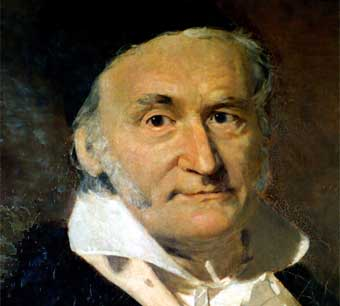
\includegraphics[width=4cm]{img-04/chap4.jpg}
	
	{\footnotesize \centering Carl F. Gauss (1777-1855) }}
{chap:complex}
  
\begin{blueshaded}
	L'home ha anat ampliant al llarg del temps la noció de nombre segons les seves necessitats. 
	
	Des de la prehistòria, els nombres naturals han servit per comptar. Els nombres enters negatius ens permeten resoldre equacions com $x+5=1$. De forma similar els nombres fraccionaris permeten resoldre $3x=2$. En l'antiga Grècia ja es sabia que no existia cap nombre racional que fos solució de $x^2=2$; D'aquí s'introduïren els nombres irracionals.
	
	El conjunt format pels nombres racionals i irracionals és el conjunt dels nombres reals. Aquests són tots els nombres amb els quals, de moment, hem treballat. 
	
%%	Existiran més tipus de nombres? Hi ha algun nombre que sigui la solució de l'equació $x^2+1=0$?
\end{blueshaded}   

\heading{Equacions de segon grau}
\begin{bluebox}
 \fontsize{10.5}{11}
  És possible trobar les solucions de l'equació $x^2-4x+13=0$?
  
  Si utilitzam la fórmula de les equacions de segon grau, trobam
  \[ x = \dfrac{4\pm \sqrt{4^2-4 \cdot 1\cdot 13}}{2} = \dfrac{4\pm \sqrt{-36}}{2} \]
  
  Donat que $\sqrt{-36}$ no és cap nombre real, deim que l'equació no té solucions reals. Però, separem  $\sqrt{-36}= \sqrt{36} \cdot \sqrt{-1} = 6 \sqrt{-1}$. Veim que el problema està en que no podem calcular $\sqrt{-1}$. 
  
  En 1777 Leonard Euler va anomenar $i=\sqrt{-1}$ com la unitat imaginària. D'aquesta forma podem escriure les solucions com:
   \[ x =  \dfrac{4\pm 6 i}{2}  = 2 \pm 3i\]
  Acabam d'escriure dos nombre complexos en forma binòmica.
\end{bluebox} 

\newpage
\section{Nombres complexos en forma binòmica}

	\begin{theorybox}
		\video[5]{164}{Introducció als nombres complexos}
			
		Es defineix la \textbf{unitat imaginària} $i$ com $i=\sqrt{-1}$. Es compleix que $i^2=-1$, $i^3=-i$, $i^4=1$, etc. \vspace{0.2cm}
		
		Els nombres de la forma $2i$, $5i$, $-\frac{3}{2}i$, $\cdots$ s'anomenen \textbf{imaginaris purs}.
 		
	 	 \begin{wrapfigure}{R}{0.2\textwidth}
	    	\vspace{-1cm} 
	    	\centering
	    	
\includegraphics[width=0.19\textwidth]{img-04/pla-complex}
		 \end{wrapfigure}
 
			Un \textbf{nombre complex} en forma binòmica s'expressa com \linebreak $z=x+iy$, on $x$ s'anomena
			\textbf{part real} i $y$ la \textbf{part imaginària} del nombre.\vspace{0.2cm}
		 
				El nombres es representen sobre el \textbf{pla complex}. A l'eix horitzontal hi situam la part
			real i a l'eix vertical la part imaginària.  \vspace{0.2cm}
			
			El \textbf{complex conjugat} del nombre s'obté de canviar el signe de la part imaginària $z^* = x-iy$. El \textbf{mòdul} d'un nombre complex és la longitud 
			del nombre i s'obté de $|z|=\sqrt{x^2+y^2}$. Es compleix que $z\cdot z^*=|z|^2$.

			\vspace{0.5cm}
	\end{theorybox}

\begin{theorybox}[Operacions en forma binòmica]
	Suposau que es donen els nombres complexos $z_1 = 2-3i$ i $z_2 = 5+4i$. Amb aquests nombres podem fer les següents operacions:
	\begin{itemize}
		\item \textbf{Suma}:  \[ z_1 + z_2 = (2-3i) + (5+4i) = 7 + i\] 
		
		\item \textbf{Resta}: \[ z_1 - z_2 = (2-3i) - (5+4i) = -3 - 7i\]
		
		\item \textbf{Producte}:  \[ z_1 \cdot z_2 = (2-3i) \cdot (5+4i) = 10+8i-15i-12 \underset{\downarrow -1}{i^2} =22 -7i \]
		
		\item \textbf{Divisió}: \[ \frac{z_1} {z_2} = \frac{(2-3i)\cdot (5-4i)}{(5+4i)\cdot(5-4i)}=\frac{-2-23i}{41}\]
	\end{itemize}
\end{theorybox}
 
\begin{mylist}
\exer
Donats els següents nombres complexos:

\begin{center}
	$a=3i$, \quad
	$b=-2i$,\quad
	$c=5$,\quad
	$d=1+i$,\quad
	$p= -1 -i$
\end{center}

\begin{tasks}
	\task Representa'ls gràficament sobre el pla complex. Representa els seus conjugats.
	\task Representa gràficament les sumes: $a+b$, \quad $a+c$, \quad $b+d$, \quad $d+p$
	\task Representa gràficament els productes: $a\cdot i$, \quad  $b\cdot i$, \quad $c\cdot i$,\quad $d\cdot i$, \quad $p\cdot i$. Comprova que multiplicar per $i$ equival a girar el nombre complex 90º.
	%\task Calcula $Im(\frac{\bar z}{z})$ (\emph{Ajuda}: substitueix $z=x+i y$)
\end{tasks} 

\answers{Nombres i conjugats:\par 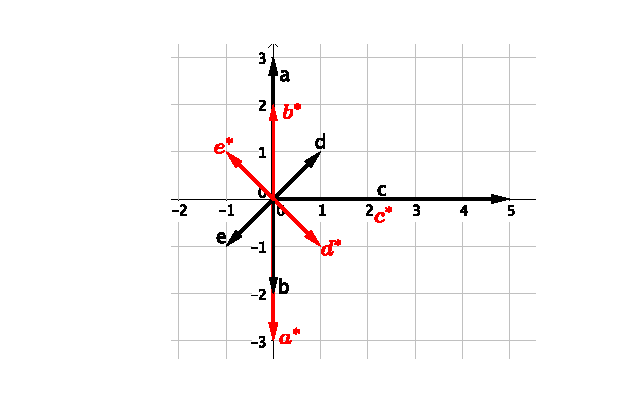
\includegraphics[width=0.44\textwidth]{img-sol/t4-1a}\par Operacions:\par 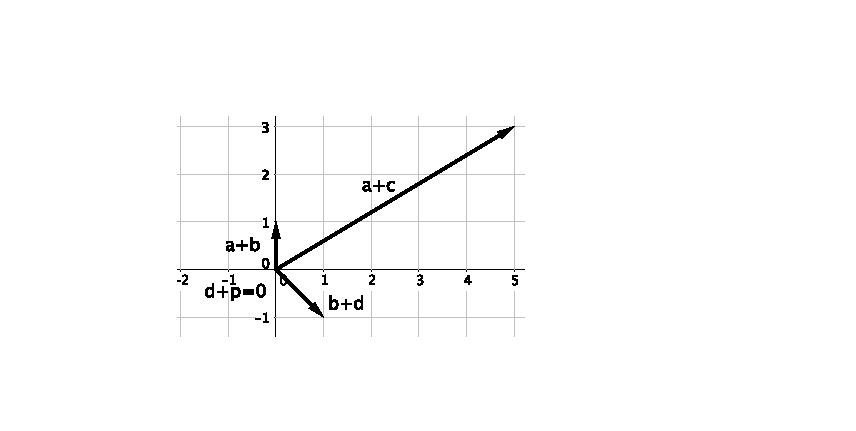
\includegraphics[width=0.44\textwidth]{img-sol/t4-1b}}
\vspace{3cm}

	\exer[1] Calcula

	\begin{tasks}(2)
		\task  $7 - 3i - (2 + 6 i)$
		\task  $(5 - 2i)\cdot (-3 i)$
		\task  $( 7 + 3 i) \cdot (-1 + 2 i)$
		\task  $(2+i)-i (1-2 i)$
		\task $(3-2 i) \cdot (3+ 2 i)$
		\task $(3 + 2i) - (1-i)\cdot(4-5i)$
	    \task $(1 + i)^2$
		\task $(1 - i)^4$
	\end{tasks}
	\answers[cols=2]{[
			 $5 -9i$,
			 $-6-15i$,
			 $-13+11i$,
			 0,
			 13,
			 $4 + 11i$,
			 $2i$,
			 $-4$]}
 ƒ
	\exer[1]
	Realitza les següents operacions amb nombres complexos:
	\begin{tasks}(2)
		\task $\dfrac{2-i}{1+3 i}$
		\task $\dfrac{5+10 i}{3-4 i}+\dfrac{2-i}{i}$
		\task $\dfrac{2+i}{4-3 i} + \dfrac{3+i}{5 i}$
		\task $\dfrac{68}{(1-i) \cdot (2-i) \cdot (3-i)}$
	\end{tasks}
\answers[cols=2]{[
		 $-{{1}\over{10}}-{{7\,i}\over{10}}$,
		 $-2$,
		 ${{2}\over{5}}-{{i}\over{5}}$,
		 ${{34\,i}\over{5}}$]}
	 
 
\end{mylist}

\begin{example}
	a) Per dividir dos nombres complexos, multiplicam i dividim pel complex conjugat del denominador.
	$\dfrac{2-i}{1+3 i} = \dfrac{(2-i)\cdot (1-3i)}{(1+3 i)\cdot (1-3i)} = \dfrac{2-6i-i-3}{10}=\dfrac{-1-7i}{10}$
	 
\end{example}


\begin{mylist}
	
	\exer Comprova les següents fórmules:
	\begin{tasks}(2)
		\task $(x+iy)^2=x^2-y^2+i2xy$
	%	\task $(x-iy)^2=x^2-y^2-i2xy$
		\task $(x+iy)\cdot (x-iy)=x^2+y^2=|z|^2$
	\end{tasks}
	

	
	\exer Calcula $a$ perquè el nombre complex $\dfrac{a+i}{3-i}$ tingui la seva part real igual a la seva part imaginària.
	\answers{Racionalitzant el nombre s'expressa com $\dfrac{3a-1}{10}+\dfrac{a+3}{10}i$. Si igualam les parts real i imaginària, això passa si $3a-1=a+3$, és a dir $a=2$}
\end{mylist}


\section{Nombres complexos en forma polar} 




\begin{theorybox}
		\video{165}{Operacions en forma polar}
	
	Un nombre complex $z=x+iy$ es pot expressar en forma polar donant el seu \textbf{mòdul} i l'angle que forma amb l'eix real.
	Aquest angle s'anomena \textbf{l'argument} del nombre complex. El nombre en \textbf{forma polar} s'expressa com $\mathbf{r_\theta}$ on
	\begin{equation*}
	r=\sqrt{x^2+y^2}, \,\,\,\,\, \,\,\,\,\,\,\,\,\,\, \theta = \arctg \dfrac{y}{x}
	\end{equation*}	
	Donat que hi ha infinits angles que tenen per tangent $y/x$, es defineix \textbf{l'argument principal} del nombre complex com un angle comprès entre $-\pi < \theta \leq \pi$ \; ($-180^\circ < \theta \leq 180^\circ$).
	
	De forma anàloga, es pot passar un nombre en forma polar a forma binòmica mitjançant
	\begin{equation*}
	z = r \cdot (\cos \theta + i \sin \theta)
	\end{equation*}	
	Aquesta forma també es coneix com \textbf{forma trigonomètrica}.
	

\end{theorybox}


\begin{mylist}
	\exer[1] Calcula el mòdul i l'argument principal dels següents nombres complexos:
	\begin{tasks}(4)
		\task  $\sqrt{3}-i$
		\task  $-2-2 i$
		\task  $1 - \sqrt{3} i $
		\task  $-4 i$
	\end{tasks}
	\answers[cols=1]{[
			 $|z|=2$;  $arg(z)=-30^\circ$,
			 $|z|=\sqrt{8}$;  $arg(z)=225 = - 135^\circ$,
			 $|z|=2$;  $arg(z)=-60^\circ$,
			 $|z|=4$;  $arg(z)=-90^\circ$]}
	
\end{mylist}
	
	\begin{example}
		a) 
		Donat $z=\sqrt{3}-i$, calculam el seu mòdul fent $|z|=\sqrt{(\sqrt 3)^2+(-1)^2}=\sqrt{4}=2$. L'argument el trobam de $\theta= \arctg(-1/\sqrt{3})=-30^\circ$.
		El nombre és $z=2_{-30^\circ}$
	\end{example}
 
 
 \begin{mylist}
 	
	\exer  
	Calcula el mòdul i l'argument principal dels següents nombres
 	complexos:

	\begin{tasks}(4)
		\task  $-3+3i$
		\task  $-3$
		\task $-3i$
		\task $3-3i$
	\end{tasks}
\answers[cols=1]{[$|z|=\sqrt{18}$;  $arg(z)=135^\circ$,
	$|z|=3$;  $arg(z)=180^\circ$,
	$|z|=3$;  $arg(z)=270^\circ$,
	$|z|=\sqrt{18}$;  $arg(z)=-45^\circ$]}


\exer Calcula l'argument principal dels següents nombres
complexos:

\begin{tasks}(3)
	\task  $\dfrac{-3}{\sqrt{3} + i}$
	\task  $\dfrac{-i}{1-i}$
	\task  $(1-i\sqrt{3})^7$
\end{tasks}
 \answers{[$z=\frac{3}{4}(-\sqrt{3}+i)$; $arg(z)=150^\circ$,
		  $z=\frac{1}{2}(1-i)$; $arg(z)=-45^\circ$,
		  $z=\left[2_{-60^\circ}\right]^7$; $arg(z)=-420^\circ=-60^\circ$]}
 
	\exer
	Expressa en forma polar els següents nombres complexos:

	\begin{tasks}(4)
		\task $i$ 
		\task $-i$
		\task $4 + 4i$ 
		\task $-4$
	\end{tasks}
\answers{[$1_{90^\circ}$, $1_{270^\circ}$, $4\sqrt{2}_{45^\circ}$, $4_{180^\circ}$]}

	
	\exer
	Expressa en forma polar els següents nombres complexos:

	\begin{tasks}(4)
		\task $5i$ 
		\task $-7i$
		\task $5 - 5i$ 
		\task $\sqrt{3}+i$

	\end{tasks}
\answers{[$5_{90^\circ}$, $7_{270^\circ}$, $5\sqrt{2}_{-45^\circ}$, $2_{30^\circ}$]}
	
	\exer[1] Expressa en forma binòmica els següents nombres complexos donats en forma polar:
	\begin{tasks}(2)
		\task De mòdul 2 i argument $\dfrac{\pi}{3}$
		\task De mòdul 3 i argument $-\dfrac{\pi}{4}$
		\task De mòdul 1 i argument $\dfrac{\pi}{2}$
		\task De mòdul 5 i argument $\dfrac{2 \pi}{3}$
	\end{tasks}
\answers[cols=1]{[ 
		 $2_{\,60^\circ}= 1 + \sqrt{3} i$, 
		 $3_{\,-45^\circ}= \frac{3\sqrt{2}}{2} - \frac{3\sqrt{2}}{2} i$, 
		 $1_{\,90^\circ}= i $, 
		 $5_{\,120^\circ}= -\frac{5}{2} + i \frac{5\sqrt{3}}{2}$]}
\end{mylist}
	
	\begin{theorybox}[Operacions en forma polar]
		L'avantatge de la forma polar és que les operacions es realitzen molt més ràpid.
		
		Si ens donen dos nombres en forma polar $r_\theta$ i $r'_{\theta'}$, 
		
		\textbf{Producte}: $r_\theta \cdot r'_{\theta'} = (r\cdot r')_{\theta+\theta'}$, multiplicam els mòduls i sumam els arguments.
		
		\textbf{Quocient}: $r_\theta : r'_{\theta'} = (r : r')_{\theta - \theta'}$, dividim els mòduls i restam els arguments.
		
		\textbf{Potència}:  $(r_\theta)^n = (r^n)_{n\cdot \theta}$, elevam el mòdul i multiplicam l'argument per l'exponent.
	\end{theorybox}
	
	\begin{resolt}[E]{Passa a forma polar, opera i comprova 
			
			$(1+i)^{16} = 2^8 = 256$.}
			En forma polar el nombre és $1+i=\sqrt{2}_{45^\circ}$. Per elevar el nombre a 16, elevam el mòdul i multiplicam l'argument per 16.
		
		\begin{equation*}
		(1+i)^{16}=(\sqrt{2}^{16} )_{16\cdot 45^\circ} = 2^8_{720^\circ}=2^8
		\end{equation*}
		
		On hem utilitzat que $720^\circ$ són dues voltes completes.
	\end{resolt}
	
\begin{mylist}	
 
	
	\exer
	Realitza les següents operacions amb nombres complexos, expressant-los

	prèviament en forma polar:

	\begin{tasks}(2)
		\task $\dfrac{\sqrt{2} i}{-2-2i}$
		\task $\left(\frac{1}{2} + \frac{\sqrt{3}i}{2}\right)^{30}$
	\end{tasks}


\answers[cols=1]{[$\dfrac{\sqrt{2} i}{-2-2i}=\dfrac{\sqrt{2}_{90}}{2\sqrt{2}_{-135}}=\dfrac{1}{2}_{225}=\dfrac{1}{2} (\cos 225 + i \sin 255)=-\dfrac{1}{4}(1+i)$, 
 $\left(\frac{1}{2} + \frac{\sqrt{3}i}{2}\right)^{30}=\left( 1_{60^\circ} \right)^{30}= 1_{1800^\circ}=1$
	]}
	
	\exer
	Realitza les següents operacions amb nombres complexos, expressant-los

	prèviament en forma polar:

	\begin{tasks}(3)
		\task $(\sqrt{3}+i)^{60}$
		\task $(4-4i)^{-11}$
		\task $\dfrac{(1-\sqrt{3} i)^{12}}{(-2-2i)^8}$
	\end{tasks}
	
	\answers[cols=1]{[$(\sqrt{3}+i)^{60}=(2_{30})^{60}=2^{60}_{1800}=2^{60}$,
		$(4-4i)^{-11}=(4\sqrt{2}_{-45^\circ})^{-11}=\frac{1}{2^{27}\sqrt{2}}_{495}=\frac{1}{2^{27}\sqrt{2}}_{135}=\frac{1}{2^{27}\sqrt{2}}(\cos 135 + i \sin 135)=\frac{1}{2^{28}} (-1+i)$,
		$\dfrac{(1-\sqrt{3} i)^{12}}{(-2-2i)^8}=\dfrac{(2_{-60^\circ})^{12}}{(2\sqrt{2}_{-135^\circ})^8}=
		\dfrac{2^{12}_{-720^\circ}}{2^{12}_{-1080^\circ}}=1_{360^\circ}=1$]}
	
\end{mylist}

\begin{theorybox}
 \textbf{Fórmula de Moivre: }
 \begin{equation*}
	(\cos \theta + i \sin \theta)^n = \cos(n \theta) + i \sin(n \theta)	 
 \end{equation*}
\end{theorybox}	
\vspace{-0.75cm}
\begin{example}
	Si utilitzam $n=2$ en la fórmula de Moivre:
	$	(\cos \theta + i \sin \theta)^2 = \cos(2 \theta) + i \sin(2 \theta) $
	
	Desenvolupam el quadrat del membre de l'esquerre:
		\[	\cos^2 \theta -  \sin^2 \theta + 2 i \sin \theta \cos \theta= \cos(2 \theta) + i \sin(2 \theta) \]
		
	Si igualam les part reals i imaginàries	trobam:
		\[ \begin{array}{l}	\cos (2\theta) = \cos^2 \theta -  \sin^2 \theta 	\\ \sin(2\theta) = 2\sin \theta \cos \theta  \end{array} \]
	que són les relacions de l'angle doble vistes en el tema \ref{chap:trig}.
\end{example}

	\begin{mylist}
		
	
	\exer Utilitza la fórmula de Moivre per expressar en funció de $\sin \theta$ i $\cos \theta$:
	\begin{tasks}(4)
		\task $\cos (-\theta)$
		\task $\sin (-\theta)$
		\task $\cos 3\theta$
		\task $\sin 3\theta$	
\end{tasks}
\answers[cols=1]{[$\cos (-\theta)=\cos \theta$, $\sin (-\theta)=-\sin\theta$, $\cos 3\theta=\cos^3 \theta - 3\sin^2 \theta \cos \theta$, $\sin 3\theta=3\sin \theta\cos^2 \theta - \sin^3\theta$]}

\end{mylist}

 
\section{Resolució d'equacions en el pla complex}
\begin{theorybox}
	\video{166}{Resolució d'equacions}
			Tot nombre complex té $n$ arrels enèsimes. Si ve expressat en forma polar $r_\theta$, les arrels són
	\begin{equation*}
		\sqrt[n]{r_\theta}= \left(\sqrt[n]{r}\right)_{\frac{\theta+k\cdot 360}{n}}
	\end{equation*}
	essent $k=0, 1, \cdots, n-1$.
	
	\vspace{0.5cm}

\end{theorybox}
	
\begin{mylist}

\exer Calcula les arrels i representa-les en el pla complex
\begin{tasks}(3)
	\task $\sqrt{-3 i}$
	\task $\sqrt{-9}$
	\task $\sqrt{1+\sqrt{3} \,i}$
	\task $\sqrt[3]{-27}$
	\task $\sqrt[3]{1-i}$
	\task $\sqrt[4]{-81}$
\end{tasks}

\answers{[$\sqrt{-3 i} \rightarrow$ $z=\pm\frac{\sqrt{6}}{2}(1-i)$ \par 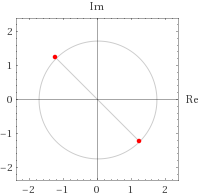
\includegraphics[width=0.3\textwidth]{img-sol/t4-15a}, 
	 $\sqrt{-9}\rightarrow$ $z=\pm 3i$ \par 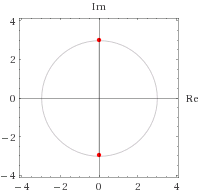
\includegraphics[width=0.3\textwidth]{img-sol/t4-15b}, 
	 $\sqrt{1+\sqrt{3} \,i}\rightarrow$ $z_1=\pm\frac{1}{2}(\sqrt{6}+i\sqrt{2})$ \par \includegraphics[width=0.3\textwidth]{img-sol/t4-15c},  
	 $\sqrt[3]{-27}\rightarrow$ $z_1=-3$; $z_2=\frac{3}{2}(1+i\sqrt{3})$; $z_3=\frac{3}{2}(1-i\sqrt{3})$ \par \includegraphics[width=0.3\textwidth]{img-sol/t4-15d}, 
	 $\sqrt[3]{1-i}\rightarrow$ $z_1\approx 1.084-0.29i$; $z_2 \approx -0.29 +1.084i$; $z_3=-0.794-0.794i$ \par \includegraphics[width=0.3\textwidth]{img-sol/t4-15e}, 
	 $\sqrt[4]{-81}\rightarrow$ $z=\pm \frac{3\sqrt{2}}{2}(1+i)$; $z=\pm \frac{3\sqrt{2}}{2}(1-i)$\par \includegraphics[width=0.3\textwidth]{img-sol/t4-15f}]}
\end{mylist}

\begin{example}
	a) Primer expressam el nombre $z=-3i$ en forma polar. Sabem que té mòdul 3 i argument 270º. Tenim dos possibles resultats de l'arrel quadrada
	\begin{equation*}
		\sqrt{3_{270^\circ}} = \left\{ 
		\begin{array}{l}
			\sqrt{3}_{270/2} = \sqrt{3}_{135^\circ} \\
			\sqrt{3}_{(270+360)/2} = \sqrt{3}_{315^\circ}
		\end{array}
		 \right.
	\end{equation*}
\end{example}


\begin{mylist}
	

\exer Calcula les arrels cinquenes de la unitat i representa-les en el pla complex. Calcula també totes les arrels cinquenes de $-1$ i representa-les.

\answers[cols=1]{[$\sqrt[5]{1} \rightarrow$ $z= 1$; $z \approx 0.309 \pm 0.9511i$; $z\approx -0.809\pm 0.5878 i$ \par \includegraphics[width=0.3\textwidth]{img-sol/t4-16a},
	$\sqrt[5]{-1} \rightarrow$ $z=-1 $; $z \approx 0.809\pm 0.588 i$; $z=-0.309 \pm 0.9511 i$ \par \includegraphics[width=0.3\textwidth]{img-sol/t4-16b}]}

	\exer Resol les equacions:
\begin{tasks}(4)
	\task $x^3=-27$
	\task $x^4=-81$
	\task $x^5+32=0$
	\task $x^3-8=0$
\end{tasks}

\answers[cols=1]{[$x=\sqrt[3]{-27}$ exemple, $x=\sqrt[4]{-81}$ exercici anterior f), $x=\sqrt[5]{-32}\rightarrow$ $z=-2$; $z\approx 1.618 \pm 1.1756 i$; $z=-0.618 \pm 1.9021 i$; \par\includegraphics[width=0.3\textwidth]{img-sol/t4-17c}, $x=\sqrt[3]{8}\rightarrow$ $z=2$; $z=-1\pm \sqrt{3}i$;\par\includegraphics[width=0.3\textwidth]{img-sol/t4-17d} ]}

\end{mylist}

\begin{example}
	a) $x^3=-27$ implica que $x=\sqrt[3]{-27}$ que evidentment té una solució real $x=-3$. Per trobar les altres dues arrels expressam el nombre en forma polar $-27=27_{180^\circ}$ i 
	en feim l'arrel cúbica.
	
	\begin{minipage}{0.7\textwidth}

	\begin{equation*}
	\sqrt[3]{27_{180^\circ}} = \left\{ 
	\begin{array}{l}
	3_{180/3} = 3_{60^\circ} \\
	3_{(180+360)/3} = 3_{180^\circ} \\
	3_{(180+2\cdot 360)/3} = 3_{300^\circ}  
	\end{array}
	\right.
	\end{equation*}
	
Si finalment passam les tres arrels a forma binòmica trobam \linebreak $x=-3$, $x=3(\frac{1}{2}+\frac{\sqrt{3}}{2}i)$, $x=3(\frac{1}{2}-\frac{\sqrt{3}}{2}i)$. Si representam aquests tres nombres sobre el pla
complex veim que formen els vèrtexs d'un triangle equilàter.
	\end{minipage}
	\begin{minipage}{0.3\textwidth}
		\begin{center}
		\includegraphics[width=0.95\textwidth]{img-04/chap-complex-3root}		
		\end{center}
	\end{minipage}

	 
\end{example}

\begin{mylist}

	\exer
	Resol les equacions, obtenint les arrels reals i complexes:

	\begin{tasks}(3)
		\task $x^2=-1$
		\task $x^3=-8$
		\task $x^4+16=0$
	\end{tasks}

\answers[cols=1]{[$x^2=-1\rightarrow$ $z=\pm i$, $x^3=-8 \rightarrow$ $z=-2$; $z=1+\sqrt{3}i$; $z=1-\sqrt{3}i$, $x^4+16=0 \rightarrow$ $z=\pm 2$; $z=\pm 2i$]}
 
	\exer
	Calcula les arrels enèsimes de la unitat, per a $n$ = 2, 3 i 4.
	Representar-les gràficament, i comprova que estan sobre la
	circumferència de radi 1, i són els vèrtexs d'un polígon regular.
	
\answers[cols=1]{[$\sqrt{1} \rightarrow$ $z=\pm 1$, $\sqrt[3]{1} \rightarrow$ $z=1$; $z=\frac{1}{2}(-1\pm \sqrt{3})$ \par \includegraphics[width=0.3\textwidth]{img-sol/t4-19b}, $\sqrt{4} \rightarrow$ $z=\pm 1$; $z=\pm i$ \par \includegraphics[width=0.3\textwidth]{img-sol/t4-19c}]}

\exer Resol l'equació $z^2+3z-1=0$.
\answers{Dues arrels reals: $z=\dfrac{-3\pm \sqrt{13}}{2}$}

	 
\exer Calcula tots els nombres complexos $z$ pels quals:
	\begin{tasks}(2)
		\task $z^6+64=0$
		\task $(z^2+3z-2)^2 - (2z^2-z+1)^2 =0$
		\task $z^6+z^5+z^4+z^3+z^2+z+1=0$
	\end{tasks}

\answers[cols=1]{[$z=\sqrt[6]{-64}$; $z=\pm 2i$; $z=\pm(\sqrt{3}+i)$; $z=\pm(\sqrt{3}-i)$, $-3z^4+10z^3-10z+3=-(z-3)(z-1)(z+1)(3z-1)$ té solucions reals $z=3$; $z=\pm 1$; $z=1/3$, Identificam una progressió geomètrica de raó $z$: La seva suma\par $\dfrac{z^7-1}{z-1}=0$ implica que $z^7=1$; són les arrels setenes de 1 (1 no serveix): Totes les arrels són per tant complexes: $z=-0.9 \pm 0.434 i$; $z=-0.22\pm 0.975 i$; $z=0.623 \pm 0.782$]}

\exer Resol aquestes equacions en el pla complex. Representa les solucions gràficament.
\begin{tasks}(2)
	\task $z^2+4i=0$
	\task $z^3+8i=0$ 
	\task $iz^3-27=0$
	\task $iz^4+4=0$
\end{tasks}

\answers{[Veure exemple;\par \includegraphics[width=0.3\textwidth]{img-sol/t4-22a}, $z=2i$; $z=-\sqrt{3}-i$; $z=\sqrt{3}-i$;\par \includegraphics[width=0.3\textwidth]{img-sol/t4-22b}, 
	$z=3i$; $z=-\frac{3}{2}(\sqrt{3}+i)$;  $z=\frac{3}{2}(\sqrt{3}-i)$;\par \includegraphics[width=0.3\textwidth]{img-sol/t4-22c}, 
	$z=\pm (1.3066+0.5412 i)$; $z=\pm (0.5412-1.3055 i)$;\par \includegraphics[width=0.3\textwidth]{img-sol/t4-22d} ]}

\end{mylist}

\begin{example}[*]
	a)  $z^2+4i=0$
	
	Començant aïllant la incògnita $z=\sqrt{-4i}$. Tot seguit hem de calcular totes les arrels (complexes) del nombre $-4i$. Per això, l'expressam en forma polar $-4i=4_{270^\circ}$.
	
	\[ \sqrt{4_{270^\circ}} = \left\{
		\begin{array}{l}
		\sqrt{4}_{\frac{270^\circ}{2}} = 2_{135^\circ} \\ 
		\sqrt{4}_{\frac{270^\circ+360^\circ}{2}} = 2_{315^\circ}
		\end{array} 
		\right.  \]
		
	Finalment, podem expressar les dues arrels en forma binòmica:
	
	\[ \left\{
	\begin{array}{l}
  2_{135^\circ} = 2 (\cos 135 + i\sin 135)= -\sqrt{2}+i\sqrt{2} \\ 
  2_{315^\circ} =  2 (\cos 315 + i\sin 315)= \sqrt{2}-i\sqrt{2}
	\end{array} 
	\right. \]
	
\end{example}

\begin{mylist}
 
\exer Calcula les quatre arrels de $z^4+9=0$ i utilitza-les per factoritzar $z^4+9$ amb dos polinomis de segon grau amb coeficients reals.
\end{mylist}


%%%%%%%%%%%%%%%%%%%%%%%%%%%%%%%%%%%%%%%%%%%%%%%%%%%%%%%%%%%
%%%%%%%%%%%%%% AUTOAVALUACIO
%%%%%%%%%%%%%%%%%%%%%%%%%%%%%%%%%%%%%%%%%%%%%%%%%%%%%%%%%%%

\begin{autoaval}{40}

\begin{mylist}
	
	\vspace{-2cm}
		
	\exer[2]  \begin{minipage}[t]{0.6\textwidth}
		Donats els nombres complexos de la figura es demana calcular:
		\begin{tasks}
			\task $z_1^* - z_3$
			\task $z_1^2$
			\task $|z_3|(z_1+z_2)$
			\task $\dfrac{z_1}{z_2}$
		\end{tasks}	
	\end{minipage}
	\begin{minipage}{0.4\textwidth}
		\centering
		\vspace{2.5cm}
		\includegraphics[width=0.7\textwidth]{img-04/autoaval-complexos1}
	\end{minipage}
\answers[cols=2]{[$-5-6i$, $-8-6i$, $10i$, $-2+i$]}

	
\exer[2]  Calcula
$\dfrac{(3+2 i)\cdot(3-2i)}{(2+3i)^3}$
\answers{$-46+63i$}

\exer[2] Resol l'equació: $z^2 - 10z+29=0$
\answers{$z_1=5+2i$, $z_2=5-2i$}

\exer[2] Donada l'expressió $\dfrac{1-i}{2-k i}$, troba els valors de $k$ pels quals l'expressió és: 
\begin{tasks}
	\task Real
	\task Imaginari pur.
\end{tasks}
\answers{[Real $k=-2$, Imaginari pur $k=-2$]}

\exer[2] Calcula el valor que ha de prendre $x$ per què el mòdul de $\dfrac{x+2i}{1-i}$ sigui igual a 2.
\answers{$x=\pm 2$}

\exer[2] Calcula el mòdul i l'argument principal del següent nombre
complex $-3 + 3i$:
\answers{$3\sqrt{2}$, $3\pi/4$}

\exer[2] Expressa en forma binòmica el nombre complex de
mòdul 2 i argument $\pi/3$
 
\answers{$1+\sqrt{3}i$}

\exer[2] Calcula $(1 + i)^6$ passant prèviament a forma polar.
 
\answers{$-8i$}

\exer[2] Expressa en forma trigonomètrica el següent nombre complex
$5i$.
\answers{$5(\cos(\pi/2) +i \sin(\pi/2)$}



\exer[2] Calcula les arrels cúbiques de $4\sqrt{3}-4i$. Representa-les gràficament.
\answers{$z_1=2_{110^\circ}$, $z_2=2_{230^\circ}$, $z_3=2_{350^\circ}$}

\end{mylist}
\end{autoaval}

\newpage
\resum
\begin{center}
\setlength\LTleft{0pt}
\setlength\LTright{0pt}
\ftimes{10.5}{11}
\renewcommand{\arraystretch}{1.5}
\fontsize{10.5}{11}
\begin{longtable}[h]{|>{\raggedleft\arraybackslash}p{0.2\textwidth}|p{0.8\textwidth}|}
	\toprule %inserts double horizontal lines
	\rowcolor{lightgray}
	
	\textbf{Apartat} & \textbf{Resum} \\   [0.5ex] 
	\toprule  \hline
	
	\cellcolor{lightgray}\noindent \textbf{Unitat imaginària} & $i^2=-1$ $\leftrightarrow$ $i=\sqrt{-1}$    \\ [0.5ex]\hline
	
	\cellcolor{lightgray}\noindent \textbf{Nombre en forma binòmica}  & $z=x+iy$ 
	
	 \sample{
	 $z=2+3i$, té part real 2 i part imaginària 3 
	 }
	  \hline
	
	\cellcolor{lightgray}\noindent \textbf{Complex conjugat} & $z^*=x-iy$ 
	
	 \sample{$\bar z = 2 - 3 i$} \hline
	
	\cellcolor{lightgray}\noindent \textbf{Suma de complexos} & $(x+iy)+(o+iv)=(x+o)+i(y+v)$ 
	
	 \sample{ $(2+3i)+(4+5i)=6+8i$ } \hline
	
	\cellcolor{lightgray}\noindent \textbf{Producte de complexos} & $(x+iy)\cdot(o+iv)=(x\cdot o - y\cdot v)+i(x\cdot v+ y \cdot o)$ 
	
	 \sample{ $(2+3i)\cdot(4+5i)=2+4i-i-2i^2=4+3i$ } \hline
	
	\cellcolor{lightgray}\noindent \textbf{Divisió de complexos} & Es multiplica numerador i denominador pel complex conjugat del denominador. Així s'aconsegueix un denominador real. 
	
	\sample{
	 $\frac{2}{1+i} = \frac{2\cdot(1-i)}{(1+i)\cdot(1-i)}=\frac{2\cdot(1-i)}{2}=1-i$  } \hline		
	
	\cellcolor{lightgray}\noindent \textbf{Forma polar} & $r_\theta$ amb $r=\sqrt{x^2+y^2}$ i $\theta=\arctg\frac{y}{x}$ 
	
	\sample{
	 $ z = 2 + 3 i$, $r=\sqrt{13}$, $\theta=\arctg \frac{3}{2}$  } \hline
	
	\cellcolor{lightgray}\noindent \textbf{Forma trigonomètrica} & $z=r\cdot(\cos\theta + i \sin \theta)$   
	
	\sample{
	 Si tenim $z=2_{30^\circ}$,  $z=2\cdot(\cos 30^\circ + i\sin 30^\circ)$  }\hline
		
	\cellcolor{lightgray}\noindent \textbf{Producte en forma polar} & $z=r_\theta$ i $z'=r'_\alpha$, aleshores $z\cdot z'= (r\cdot r')_{\theta+\alpha}$. Multiplicam els mòduls i sumam els arguments.   
	
	\sample{ Si tenim $z=2_{30^\circ}$ i $z'=3_{50^\circ}$,   $z\cdot z'=(2\cdot 3)_{30+50^\circ}=6_{80^\circ}$  } \hline
		
	\cellcolor{lightgray}\noindent \textbf{Divisió en forma polar} & $z=r_\theta$ i $z'=r'_\alpha$, aleshores $z / z'= (r / r')_{\theta-\alpha}$. Dividim els mòduls i restam els arguments.
	   
	\sample{ Si tenim $z=2_{30^\circ}$ i $z'=3_{50^\circ}$,   $z / z'=(2 / 3)_{30-50^\circ}=(2/3)_{340^\circ}$  } \hline	
	
	\cellcolor{lightgray}\noindent \textbf{Potència en forma polar} & $z=r_\theta$, aleshores $z^n= (r^n)_{n\cdot\theta}$. Elevam el mòdul i multiplicam l'argument per $n$.   
	
	 \sample{ Si tenim $z=2_{30^\circ}$ i volem calcular  $z^3= (2 ^ 3)_{3\cdot 30^\circ}=8_{90^\circ}$  } \hline	
		
	\hline \bottomrule
\end{longtable}
\end{center}
  
 
%%%%% Activitats de bloc 1
\partsintesi{Síntesi de la Part I}{Aritmètica, Àlgebra i Trigonometria}


\begin{mylist}
	
\exer[2] Efectua les operacions següents i simplifica:
\begin{tasks}
	\task $\sqrt{a^3} - 2a \sqrt[4]{a^2} + 3a \sqrt[6]{a^3} - \sqrt[8]{a^{12}}$
	\task $\dfrac{5}{\sqrt{6}} + \dfrac{2}{\sqrt{6}+3\sqrt{2}} - \dfrac{4\sqrt{2}}{\sqrt{3}}$
\end{tasks}
\answers{a) $a\sqrt{a}$ \quad \quad b) $\frac{3\sqrt{2}-4\sqrt{6}}{6}$}

\exer[2] Efectua les operacions següents i simplifica:
\begin{tasks}(2)
	\task $\left( \sqrt[4]{a^3} \cdot \sqrt[5]{a^4} \right): \sqrt{a}$
	\task $\dfrac{4+\sqrt{6}}{2\sqrt{3}}  -  \dfrac{2}{3-\sqrt{3}}$
\end{tasks}
\answers{a) $a\,\sqrt[20]{a}$ \quad \quad b)$\frac{2\sqrt{3}+3\sqrt{2}-6}{6}$}

\exer[2] Factoritza el polinomi $3x^5 - 4x^4 - 5x^3 + 2x^2$
\answers{$x^2 (x+1) (x-2) (3x-1)$}

\exer[2] Opera i simplifica $\left( \dfrac{x^2-4}{x+1} : \dfrac{x^2+2x}{x^3-x} \right) - (x^2-3x)$
\answers{2}

\exer[2] Resol l'equació $\sqrt{2x+3} - 2x = x-6$
\answers{$x=3$ vàlida.}

\exer[2] Resol l'equació $\dfrac{7-x}{x^2+4x+4} + \dfrac{x}{x+2}=1$
\answers{$x=1$}

\exer[2] Resol el sistema d'inequacions $\left\{ \begin{array}{l} 
x+1-3(x-1)<1-x \\ x^2-x-6\ge 0 
\end{array}\right.$
\answers{$(3, +\infty)$}

%\exer[2] Resol pel mètode de Gauss $\left\{ \begin{array}{ll} 
%x+2y+z &=1 \\ -2x+y-z &= -5 \\ 3x-y+3z &=10 
%\end{array}\right.$
%\answers{$x=2$, $y=-1$, $z=2$}

\exer[2] Un examen consisteix en un test de 60 preguntes. Per cada encert obtens 5 punts, per cada errada et lleven 2 punts i per cada pregunta no contestada resta 1 punt. Quantes preguntes bé, malament i en blanc va contestar un alumne sabent que va obtenir 150 punts i que el nombre d'errades més el quíntuple de les no contestades va ésser igual al nombre d'encerts? 
\answers{$x=38$: be, $y=18$: malament, $z=4$: no contestades. Planteig: $x+y+z=60$; $5x-2y-z=150$; $y+5z=x$}

\exer[2] Resol pel mètode de Gauss i classifica el sistema $\left\{ \begin{array}{ll} 
2x+y-z &=-1 \\ x-y+z &= 4 \\ 4x-y+z &=7 
\end{array}\right.$
\answers{S.C.I. $x=1$, $y=z-3$, $z=z$}

\exer[2] Les diagonals d'un paral·lelogram mesuren 16 cm i 28 cm i formen un angle de 48º. Calcula el perímetre i l'àrea d'aquest paral·lelogram.
\answers{Els costats són 10.49 cm i 20.25 cm, el perímetre 61.48 cm. L'àrea 83.23 cm$^2$.}
 
\exer[2] Tenim un triangle de perímetre 48 cm. Sabent que el costat major supera en 6 unitats el menor i que l'altre costat és la mitjana aritmètica del major i del menor, calcula els angles d'aquest triangle.
\answers{Primer obtenim els costats resolent un sistema d'equacions $a=19$,  $b=16$ i $c=13$. Després aplicam el Teorema del Cosinus per obtenir els angles $\hat A=42.54^\circ$, $\hat B=56.3^\circ$, $\hat C=81.17^\circ$}

\exer[2] 
\begin{minipage}[t]{0.55\textwidth}
Per construir un túnel entre dues ciutats $A$ i $C$ necessitam saber la seva longitud i direcció. Per això, fixam un punt $B$ i prenem les mesures indicades en la figura. Calcula $\bar{AC}$ i els angles $\hat B$ i $\hat C$.
\end{minipage}
\begin{minipage}[c]{0.5\textwidth}
\begin{center}
	\includegraphics[width=5cm]{img-04-bloc1/bloc1-fig1.png}
\end{center}
\end{minipage}
\answers{Utilitzam el Teorema del Sinus. $\hat C= 56^\circ \, 19^\prime \, 31^{\prime\prime}$, $\hat B= 51^\circ \, 40^\prime \, 29^{\prime\prime}$ i  $\bar{AC}=263.96$ m.}

\exer[2] Una nau espacial es troba sobrevolant el pol nord de la Terra a una certa distància $d$ de la seva superfície. Si volem veure els continents fins a una latitud de $40^\circ$ nord, quina és l'altura mínima ha de volar la nau? Preneu radi de la Terra $R=6400$ km.
\answers{$d=3557$ km sobre la superfície de la Terra.} 

\exer[2] Justifica si existeix algun angle $a$ pel qual $\tg a=\frac{2}{3}$ i $\sin a = \frac{1}{2}$.
\answers{No existeix cap angle amb aquestes condicions. S'obtindria que $\cos a = 3/4$ i amb aquesta dada no es compleix que $\sin^2 a +\cos^2 a = 1$.}

\exer[2] Sabent que $\tg \alpha= 2$ i que $\cos \alpha>0$, troba:
\begin{tasks}(4)
	\task $\cos 2\alpha$
	\task $\sin(\frac{\pi}{2}-\alpha)$
	\task $\sin \frac{\alpha}{2}$
	\task $\tg (\frac{\pi}{4}+\alpha)$
\end{tasks}
\answers{En primer lloc trobam que $\sin \alpha = \frac{2\sqrt 5}{5}$ i $\cos \alpha = \frac{\sqrt 5}{5}$. 	a) $-3/5$ \quad   b) $\frac{\sqrt 5}{5}$ \quad  c)  $\sqrt{\frac{5-\sqrt 5}{10}}$ \quad  d) $-3$}

\exer[2] Demostra les següents identitats trigonomètriques
\begin{tasks}
	\task $\cos^4 \alpha - \sin^4 \alpha = 2 \cos^2 \alpha -1$
	\task $2 \tg \beta \cdot \cos^2 \frac{\beta}{2}-\sin\beta = \tg \beta$
\end{tasks}
\answers{a) Utilitza que $sin^4 x = (1-\cos^2 x)^2$ desenvolupa el quadrat i simplifica.
	b) Utilitza que $\cos^2 \frac{\beta}{2} = \frac{1+\cos \beta}{2}$
}

\exer[2] Resol aquestes equacions trigonomètriques
\begin{tasks}
	\task $2\sin x + \cos x = 1$
	\task $2 \sin^2 \frac{x}{2} + \cos 2x = 0$
\end{tasks}
\answers{a) $x= 0^\circ+ n\cdot 360^\circ$, $x=126.87^\circ+ n\cdot 360^\circ$. 
	b) $x= 90^\circ+ n\cdot 180^\circ$, $x= 60^\circ+ n\cdot 360^\circ$, $x= 300^\circ+ n\cdot 360^\circ$.}

\exer[2] Resol $\left\{ \begin{array}{l}  
\sin 3x + \sin y = \frac{3}{2} \\ 
\cos \left(  \frac{3x-y}{2} \right) = \frac{\sqrt{3}}{2}
\end{array}\right.$
\answers{$x=30^\circ + n\cdot 180^\circ$, $y=30^\circ + k\cdot 180^\circ$.}

\exer[2] Efectua $\dfrac{(3-2i)^2 - (1+i)(2-i)}{-3+i}$
\answers{$-\frac{19}{10}+\frac{37}{10}i$}

\exer[2] Simplifica $\dfrac{i^{10} - 2 i^7}{2 + i^{33}}$. \emph{Ajuda: Recorda quines són les potències de} $i$.
\answers{$i$}

\exer[2] Resol l'equació en el conjunt dels nombres complexos $z^2-10z+29=0$.
\answers{$z=5+2i$, $z=5-2i$}

\exer[2] Donat el nombre complex $z=3_{\, 60^\circ}$, expressa en forma polar $z^*$, $1/z$, $z^2$, $\sqrt[3]{z}$. 
\answers{ $z^*=3_{\, 300^\circ}$, $1/z=(1/3)_{\, 300^\circ}$, $z^2=9_{\, 120^\circ}$, $\sqrt[3]{z}$ té tres resultats = $(\sqrt{3})_{\, 20^\circ}$, $(\sqrt{3})_{\, 140^\circ}$ i $(\sqrt{3})_{\, 260^\circ}$.}
\end{mylist}


\mypart[L'anàlisi de sèries temporals és cabdal en la vida quotidiana.]{ANÀLISI DE FUNCIONS}{img-00/bloc2}
 
\vspace*{\fill}
\begin{center}
	\includegraphics[width=0.65\textwidth]{img-00/bloc2-historia}
\end{center}
\vspace*{\fill} 
 
\mychapter{Funcions elementals}{Funcions elementals}{
\includegraphics[width=4.5cm]{img-05/chap6.jpg}
}{chap:elemental}

 \vspace*{\fill}
 
\begin{blueshaded}
	
	{\Large \textbf{Una breu història}}
	
	
	\begin{wrapfigure}{R}{4cm}
		\begin{center}
		\includegraphics[width=3cm]{img-05/leibniz.jpg}	
		{\footnotesize
		Gottfried Leibniz va introduir el terme «funció» en el segle XVII.}
		\end{center}
	\end{wrapfigure}
	El concepte de funció com el coneixem avui en dia, va aparèixer amb als inicis del càlcul en el segle XVII. René Descartes, Isaac Newton i Gottfried Leibniz van establir la idea de funció com la dependència entre dues quantitats. Leibniz, en particular, va introduir els termes «Funció», «variables», «constant» i «paràmetre». La notació $f(x)$ va ser utilitzada per primera vegada per A.C. Clairaut i per Leonhard Euler en la seva obra {\normalfont \textit{Commentarii de Sant Petersburg}} en 1736.
	
	Inicialment, una funció $f$ s'identificava a efectes pràctics amb una expressió analítica que permetia calcular els seus valors. No obstant això, aquesta definició tenia algunes limitacions: Expressions analítiques diferents podien donar lloc a valors numèrics iguals. En 1837, Dirichlet va proposar la definició moderna de funció com una correspondència entre dos conjunts de nombres, que associa a cada nombre del conjunt de sortida un únic nombre del conjunt d'arribada.
	 
\end{blueshaded}


 \vspace*{\fill}
 
\newpage
\heading{Prova inicial}

Associa a cada gràfica una equació de les que es presenten a continuació.

\includegraphics[width=\textwidth]{img-05/chap6-inicial.png}

\addanswersline[cols=1]{Avaluació inicial}{0}{
\begin{tasks}(4)
	\task L$_{4}$	\task R$_3$		\task L$_2$		\task C$_4$
	\task PI$_{2}$	\task E$_3$		\task C$_1$		\task E$_1$
	\task L$_{1}$	\task PI$_4$		\task PI$_3$		\task R$_2$
\end{tasks}
\par
No tenen gràfica associada L$_3$, C$_2$, C$_3$, PI$_1$, R$_1$, R$_4$, E$_2$ i E$_4$. 
}

\section{Concepte de funció}

\begin{theorybox}
	$f: Dom \rightarrow Rec$ és una funció si per a cada $x$ del domini $Dom$ associa \textbf{un únic} valor $y$ del recorregut $Rec$. S'anomena $y=f(x)$, la imatge de $x$ per la funció $f$.
	
	Si $Dom\, f$ són els nombres naturals, parlam de \textbf{successions}.
	
	Si $Dom\, f$ és el conjunt dels nombres reals, parlam de \textbf{funcions de variable real}.
	
	
	Per representar funcions utilitzam uns eixos cartesians on col·locam $x$ sobre l'eix horitzontal (\textbf{abscisses}) i $y$ sobre l'eix vertical (\textbf{ordenades}).
\end{theorybox}

\subsection{Successions}
\begin{theorybox}
	Una successió és una llista ordenada de nombres reals que anomenam termes:
	\[ a_n : a_1, a_2, a_3, \cdots \]
	
	Una successió es pot expressar:
	\begin{itemize}
		\item Donant els primers termes: $1, 3, 5, 7, \cdots$
		\item Donant el terme general: $a_n = 2n-1$
		\item Donant una relació de recurrència: $a_1 = 1$ i $a_{n+1}=a_n+2$
	\end{itemize}
\end{theorybox}

\begin{mylist}
\exer[1]	Troba els 7 primers termes de la successió $a_1=2$, $a_2=3$, $a_n=a_{n-1
	}+a_{n-2}$.	
\answers{2, 3, 5, 8, 13, 21, 34, ...}

\exer[1] Dóna el terme general o la relació de recurrència de les successions:
\begin{tasks}
	\task $3, 8, 13, 18, 23, \cdots$
	\task $1, 8, 27, 64, 125, \cdots$
	\task $8, 4, 2, 1, \cdots$
\end{tasks}

\answers{a) $a_n=3+5(n-1)$ o $a_1=3$ $a_n=a_{n-1}+3$ \par b) $a_n=n^3$ \par c) $a_n=8\cdot (1/2)^{n-1}$ o $a_1=8$ $a_n=a_{n-1}/2$]}
\end{mylist}

\begin{theorybox}[Progressions aritmètiques]
	Una progressió aritmètica és una successió en la qual la diferència $d$ entre dos termes consecutius es manté constant.
	
	El terme general és: $a_n = a_1 + d \cdot (n-1)$.
	
	La suma dels $N$ primers termes és: $S_N = \dfrac{a_1+a_N}{2} \cdot N$
\end{theorybox}
 

\begin{theorybox}[Progressions geomètriques]
		Una progressió geomètrica és una successió en la qual el quocient (anomenat raó $r$)  entre dos termes consecutius es manté constant.
	
	El terme general és: $a_n = a_1 \cdot r^{n-1}$.
	
	La suma dels $N$ primers termes és: $S_N = a_1 \dfrac{r^N-1}{r-1}$
	
	Si $|r|<1$, la progressió és decreixent i la suma dels infinits termes és: $S_\infty = \dfrac{a_1}{1-r}$
\end{theorybox}

\begin{mylist}
	\exer[1] Troba el terme 100 de la progressió $10, 7, 4, 1, -2, \cdots$.
	\answers{$a_n=10-3(n-1)$ i $a_{100}=-197$}
	
	\exer[1] D'una progressió aritmètica coneixem $a_3=11$ i $a_5=19$. Calcula el terme general i la suma dels 100 primers termes.
	\answers{$d=(19-11)/2=4$ i $a_1=3$, \linebreak $a_n=3+4(n-1)$, $S_{100}=20100$}
	
	\exer[1] Troba el terme 50 de la progressió $100, 50, 25, 12.5, \cdots$. Troba la suma dels infinits termes.
	\answers{$a_n=100\cdot(0.5)^{n-1}$, $a_{50}=1.776\cdot 10^{-13}$, $S_\infty=200$}
	
	\exer[1] Calcula la suma dels 30 primers termes d'una progressió geomètrica amb termes \linebreak $a_2=3$ i $a_5=81$.
	\answers{$r=3$ i $a_1=1$, $a_n=3^{n-1}$, $S_{30}=1.029\cdot 10^{14}$}
	
\end{mylist}

\subsection{Funcions de variable real}

\begin{mylist}

\begin{minipage}[T]{0.58\textwidth}
	\exer Quines d'aquestes gràfiques representen funció i quines no? Explica per què?	
\end{minipage}
\begin{minipage}{0.38\textwidth}
	\noindent \includegraphics[width=0.85\textwidth]{img-05/fe-is-func}	
\end{minipage}
 \answers{Són funcions 2 i 4. No són funcions 1 i 3, perquè per un mateix valor de $x$ trobam més d'un valor de $y$ ``La gràfica té plegaments''.}	

\exer \mental Observa les gràfiques d'aquestes funcions i indica quin és el seu domini de definició i el seu recorregut:	

\noindent \includegraphics[width=0.93\textwidth]{img-05/fe-dom-rec}	
\answers{[Dom $f=[-4,4]$, Dom $f=(-\infty,3)]$, Dom $f=(-\infty,-2)\cup(-2,2)\cup (2,+\infty)$ o també  Dom $f=\Re-\{-2,2\}$, Dom $f=[-2,5]$]}
\end{mylist}

\begin{theorybox}
	Totes les funcions polinòmiques tenen com $Dom f=\mathbb{R}$. Però, hi ha situacions en què el domini es troba limitat perquè és impossible calcular la funció.
	\begin{itemize}
		\item No és possible dividir entre zero.
		\item No es pot calcular l'arrel quadrada d'un nombre negatiu.
		\item No existeix el logaritme de zero ni d'un nombre negatiu.
		\item No té sentit físic; per exemple no existeixen àrees negatives.
	\end{itemize}
\end{theorybox}

\begin{resolt}[E]{Calcula el domini de \par
		  $y=\dfrac{x}{x^2-4}$
	}
  El denominador és igual a zero quan $x=\pm 2$, el domini són tots els nombres reals excepte aquests dos: $Dom\, f=\mathbb{R}-\{-2,2\}$
\end{resolt}  
\vspace{-0.75cm}
\begin{resolt}{Calcula el domini de 	\begin{equation*}
	y=\sqrt{3-x}
		\end{equation*}  }
 El radicand ha d'esser major o igual a zero $3-x \geq 0$. La solució d'aquesta inequació és $x\leq 3$ o en forma d'interval $Dom\, f=(-\infty, 3]$
\end{resolt}  
\vspace{-0.75cm}
\begin{resolt}{Calcula el domini de 	\begin{equation*}
	y=\sqrt{\dfrac{x+2}{x-1}}
		\end{equation*}}
	  En primer lloc el denominador no pot ésser zero; llavors $x=1$ queda descartat. En segon lloc, el radicand ha d'esser major o igual a zero. Per això analitzam els signes del numerador i denominador:
	\begin{center}
		\includegraphics[width=0.32\textwidth]{img-05/chap-fe-domsignes.png}
	\end{center}
	
	El signe de la divisió ha de donar positiu o zero, aleshores $Dom f=(-\infty, -2] \cup (1, +\infty)$.
\end{resolt}

\begin{mylist} 
	
	
	\exer[1]  Calcula en el teu quadern el domini de les següents funcions:
	
	
	\begin{tabular}{|p{0.2in}|p{0.9in}|p{1.3in}|p{0.2in}|p{0.8in}|p{1.4in}|} \hline 
		\multicolumn{2}{|p{1in}|}{\textbf{Funció}} & \textbf{Domini} & \multicolumn{2}{|p{1.0in}|}{\textbf{Funció}} & \textbf{Domini} \\ \hline 
		\textit{f} & $\dfrac{5x^{2} +1}{x^{2} -4} $ &  &  \textit{j} & $\sqrt{\frac{x+3}{x-3} } $ &  \\ \hline 
		\textit{g} & $\sqrt{\frac{3x+2}{x-3} } $ &  &  \textit{k} & $\dfrac{2x^{2} -1}{x^{2} -3} $ &  \\ \hline 
		\textit{h} & $\dfrac{x+1}{x-1} $ &  &  \textit{l} & $\sqrt{\frac{x+2}{3-x} } $ &  \\ \hline 
		\textit{i} & $\dfrac{x^{2} +1}{x^{2} -1} $ &  &  \textit{m} & $\dfrac{x+1}{x-1} $ &  \\ \hline 
	\end{tabular}
\answers{$\text{Dom }f=\Re-\{\pm 2\}$,\par $\text{Dom } g=(-\infty,-2/3]\cup (3,+\infty)$,\par $\text{Dom } h=\Re-\{1\}$,\par $\text{Dom } i=\Re-\{\pm 1\}$,\par $\text{Dom } j=(-\infty,-3]\cup(3,+\infty)$,\par $\text{Dom } k=\Re-\{\pm \sqrt{3}\}$,\par $\text{Dom } l=[-2,3)$, $\text{Dom } m=\Re - \{1\}$}
	
\exer Calcula en el teu quadern el domini de cadascuna de les següents funcions:
\[\begin{array}{lll} 
p(x)=-5x+3;&q(x)=\sqrt{2x^{2} -x+7}&;r(x)=\sqrt[{4}]{-x^{3} -1} \\ s(x)=\sqrt[{3}]{3x^{2} -x};&f(x)=\dfrac{2x-4}{x+3};&\quad g(x)=\dfrac{-3}{x} \\ 
h(x)=\dfrac{x+1}{x^{2} +1};& j(x)=\dfrac{-x^{2} +2x}{x^{2} -4}& \end{array}\] 
 
\begin{tabular}{|p{0.2in} p{0.6in}|p{1.5in}|p{0.3in} p{0.6in} | p{1.6in}|} \hline 
\multicolumn{2}{|p{1in}|}{Funció} & Domini & \multicolumn{2}{|p{0.9in}|}{Funció} & Domini \\ \hline 
\textit{} & $p(x)$ &  &  \textit{} & $q(x)$ &  \\ \hline 
\textit{} & $r(x)$ &  &  \textit{} & $s(x)$ &  \\ \hline 
\textit{} & $f(x)$ &  &  \textit{} & $g(x)$ &  \\ \hline 
\textit{} & $h(x)$ &  &  \textit{} & $j(x)$ &  \\ \hline 
\end{tabular}

\answers{Dom $p=\Re$;\par Dom $q=\Re$;\par Dom $r=(-\infty,-1]$;\par Dom $s=\Re$;\par Dom $f=\Re-\{-3\}$;\par Dom $g=\Re-\{0\}$;\par Dom $h=\Re$;\par Dom $j=\Re-\{-2,2\}$ }

\exer Sigui la funció donada per $f\left(x\right)=x^{3} +ax^{2} +bx+c$. Determina $a$, $b$ i $c$ sabent que la funció té simetria senar i que passa pel punt (1, $-2$).

\answers{Si és senar $a=0$ i $c=0$. Si passa per $(1,-2)$ implica que $b=-3$}

\exer  Les dades de la taula indiquen en la primera fila, els preus, en euros, per sac de taronges, en la segona fila, les quantitats demandades de taronges per setmanes, i en la tercera fila, les quantitats ofertes:

\begin{tabular}{|p{2.4in}|p{0.6in}|p{0.6in}|p{0.6in}|p{0.6in}|} \hline 
	Preu per sac (euros) & 8 & 6 & 4 & 2 \\ \hline 
	Quantitat demandada (milers de sacs per setmana) & 50 & 100 & 200 & 400 \\ \hline 
	Quantitat oferta (milers de sacs per setmana) & 300 & 250 & 200 & 100 \\ \hline 
\end{tabular}

Dibuixa una gràfica amb les dades d'aquesta taula, representant en l'eix vertical els preus, i en l'eix horitzontal les quantitats demandades i ofertes. Uneix amb un traç continu ambdues corbes.

\answers{Gràfica:\par \includegraphics[width=0.4\textwidth]{img-sol/t5-12}}

\exer  Les dades de la taula indiquen en la primera fila, els preus, en euros, del lloguer d'un pis de 70 m${}^{2}$, en la segona fila, la quantitat de persones que desitgen llogar un pis, i en la tercera fila, els pisos buits en una determinada ciutat:


\begin{tabular}{|p{2.5in}|p{0.6in}|p{0.6in}|p{0.6in}|} \hline 
	Preu d'un pis (euros) & 1500 & 1000 & 500 \\ \hline 
	Quantitat demandada (persones que desitgen llogar) & 10 & 100 & 500 \\ \hline 
	Quantitat oferta (pisos lliures) & 600 & 200 & 50 \\ \hline 
\end{tabular}

\begin{tasks}
	\task  Dibuixa una gràfica de les corbes d'oferta i demanda.
	%%
	\task  Determina de forma aproximada el punt d'equilibri
\end{tasks}

\answers{a) Gràfica:\par \includegraphics[width=0.4\textwidth]{img-sol/t5-13}\par b) El punt d'equilibri és quan l'oferta iguala la demanda. Això passarà per una oferta de 175 pisos  un preu per pis de 910 \euro{}.}



\end{mylist}

\section{Funcions elementals}
\vspace{-0.6cm} 
\subsection{Lineals i Quadràtiques}
\vspace{-0.4cm}
\begin{theorybox}[Funció lineal]
	L'expressió d'una funció lineal és $y=mx+n$, essent $m$ el pendent i $n$ l'ordenada a l'origen. Si $m=0$ es diu que la funció és constant i la gràfica és una recta horitzontal.
\end{theorybox}

\begin{theorybox}[Funció quadràtica o paràbola]
	L'expressió d'una funció quadràtica és $y=ax^2+bx+c$. Quan $a>0$ la funció és còncava $\cup$ i si $a<0$ és convexa $\cap$. El valor de $b$ controla la posició del vèrtex. L'abscissa del vèrtex s'obté de la fórmula $x_v=\dfrac{-b}{2a}$. L'ordenada del vèrtex es troba substituïnt $x_v$ dins la funció.
\end{theorybox}


\begin{mylist}
\exer Calcula el vèrtex i punts de talls amb els eixos de les següents paràboles. Representa-les gràficament:
\begin{tasks}(3)
	\task $y=-x^2+2x-3$
	\task $y=x^2+2x+1$
	\task $y=x^2-6x+5$
	\task $y=\frac{1}{3}x^2-x+3$
	\task $y=\frac{1}{4}x^2+x-2$
	\task $y=2x^2-10x+8$
\end{tasks}

\answers{Gràfica: \par \includegraphics[width=0.4\textwidth]{img-sol/t5-14}}

\exer Un objecte es llança verticalment cap amunt des d'un determinat punt. L'altura en metres aconseguida al cap de $t$ segons, ve donada per $h(t)=5+4t-t^{2}$. Calcula l'altura des de la qual es llança l'objecte i a la qual es troba després d'1 segon. Determina en quin instant aconseguirà l'altura màxima i quina és. Finalment, calcula l'instant en què caurà al terra i representa gràficament la situació amb les dades obtingudes anteriorment.

\answers{L'objecte es llança des d'una altura de 5 m. Al cap d'1 s està a 8 m. Assoleix una altura màxima de 9 m als 2 s. Arriba al terra als 5 segons.\par \includegraphics[width=0.4\textwidth]{img-sol/t5-15}}

\exer La despesa pel consum de llum (en cèntims d'euro) d'un habitatge, en funció del temps transcorregut (en hores), ens ve donada per l'expressió $f\left(t\right)\, \, =\, \, -\frac{1}{5} t^{2} +2t+10$ per a $0\le t\le 12$.

\begin{tasks}
\task Representa gràficament la funció.
\task Quin és el consum a les 6 hores? I després de 12 hores? 
\end{tasks}

\answers{a) \par \includegraphics[width=0.4\textwidth]{img-sol/t5-16} \par b) $f(6)=14.8$ i $f(12)=5.2$ cèntims.}

\end{mylist}

\subsection{Funcions arrel}

\begin{mylist}
 \exer Representa gràficament les funcions:
 \begin{tasks}(4)
 	\task $y=\sqrt{x-1}$
 	\task $y=-\sqrt{x+3}$
 	\task $y=2+\sqrt{x}$
 	\task $y=1-\sqrt{x}$
\end{tasks}
\answers{\mbox{}\par \includegraphics[width=0.4\textwidth]{img-sol/t5-17}}

\end{mylist}

\subsection{Proporcionalitat inversa (Hipèrboles)}
\begin{mylist}
 \exer Representa gràficament les funcions:
\begin{tasks}(4)
	\task $y=\dfrac{1}{x+1}$
	\task $y=\dfrac{1}{x-1}$
	\task $y=\dfrac{-1}{x}$
	\task $y=\dfrac{-1}{x-3}$
\end{tasks}
\answers{\mbox{}\par \includegraphics[width=0.4\textwidth]{img-sol/t5-18}}

\exer Dibuixa el recinte limitat pels semieixos positius de coordenades i les corbes $y=x^{2} +1,{\rm \; }y=\dfrac{2}{x} $ i  $y=x-1$.
\answers{\mbox{}\par \includegraphics[width=0.4\textwidth]{img-sol/t5-19}}

\exer Els beneficis d'una empresa, en milers d'euros, s'ajusten a la funció $f\left(x\right)=\dfrac{50x-100}{2x+5} $, on $x$ representa els anys de vida de l'empresa, essent $x\ge 0$. Calcula el domini, tall amb els eixos, signe i simetries d'aquesta funció.

\answers{Dom $f=[0,+\infty]$. Tall eix OX $(2,0)$;  Tall eix OY $(0,-20)$. No presenta simetries. La funció és negativa a $[0,2)$ i positiva a $(2,+\infty)$.}
\end{mylist}

\subsection{Funció a trossos i valor absolut}
\begin{mylist}
	\exer  Representa gràficament la funció valor absolut $y=|x|$. Expressa-la com una funció a trossos.
	
	\answers{$|x|=\left\{ \begin{array}{ll}
		-x & \text{ si } x<0 \\
		 x & \text{ si } x\ge 0 
		\end{array} \right.$}
	
	\exer  Representa les següents funcions a trossos. 
	
	\begin{tasks}
	\task  $f(x)=\left\{\begin{array}{cl} x^{2} -1\; \; \; \;& si\; \; x<-4 \\ -x+2\; \; \; \;& si\; \; -4\le x<0 \\ 5\; \; \; \;& si\; \; \; \; 0\le x \end{array}\right. $  
	%
	\task  $g(x)=\left\{\begin{array}{cl} \frac{1}{x} \; \;& si\; \; x<-3 \\ x\; \; \; & si\; \; -3\le x<2 \\ \sqrt{x} \; \; \; \;& si\; \; 2\le x \end{array}\right. $  
	%
	\end{tasks}
\answers{\mbox{}\par \includegraphics[width=0.4\textwidth]{img-sol/t5-22a}\par
\includegraphics[width=0.4\textwidth]{img-sol/t5-22b}}


\exer Esbossa la gràfica de la funció $f$: $\Re$ $\rightarrow$ $\Re$ donada per $f(x)=\left\{\begin{array}{l} {2x+2\quad {\rm si\; \; }x\le -1,} \\ {x^{3} -x\quad {\rm si\; \; }x>-1.} \end{array}\right. $
\answers{\mbox{}\par \includegraphics[width=0.4\textwidth]{img-sol/t5-23}}

\exer Siguin les funcions definides mitjançant $f(x){\rm \; }=\left|x\left(x-2\right)\right|$ i  $g(x)=x+4$. Representa les gràfiques de $f$ i $g$ sobre els mateixos eixos i calcula els punts de tall entre ambdues.
\answers{\mbox{}\par \includegraphics[width=0.4\textwidth]{img-sol/t5-24}}

\exer Representa les següents funcions i defineix-les com a funcions a trossos:
\begin{tasks}(4)
	\task $y=|4-x|$
	\task $y=|3x+6|$
	\task $y=|x^2-1|$
	\task $y=|x^2+2x-3|$
\end{tasks}
\answers{\mbox{}\par \includegraphics[width=0.4\textwidth]{img-sol/t5-25}}

\exer Sigui la funció $f(x)=\left\{\begin{array}{l} {1-x^{2} } \\ {3x^{2} -12x+9} \\ {-2x^{2} +16x-30} \end{array}{\rm \; \; \; \; }\begin{array}{c} {{\rm si}} \\ {{\rm si}} \\ {{\rm si}} \end{array}\right. {\rm \; \; \; }\begin{array}{l} {x\le 1} \\ {1<x\le 3} \\ {x>3} \end{array}$. Dibuixa la seva gràfica i, a partir d'ella, indica el seu domini, els  punts de tall amb els eixos i el seu signe.
\answers{\mbox{}\par \includegraphics[width=0.4\textwidth]{img-sol/t5-26}}

\end{mylist}

\pagebreak
\subsection{Funció exponencial}

\begin{theorybox}
	Les funcions exponencials són del tipus $y=a^x$. Si $a>1$ són creixents i si $0<a<1$ són decreixents. Totes elles passen pel punt $(0, 1)$.
	
	Un cas important és $y=e^x$ on la base és el número $e \simeq 2.7182818$.
\end{theorybox}

\begin{mylist}
\exer  En el teu quadern, representa conjuntament les gràfiques de $y=f(x)=x^2$ (funció potencial) i $f(x)=2^x$ (funció exponencial), amb valors de ``\textit{x}'' entre 0 i 5. Observa la diferència quantitativa entre el creixement potencial i el creixement exponencial. 

\exer Dibuixa el recinte limitat per les corbes $y=e^{x+2} ,$ $y=e^{-x} $  i  $x=0.$
\answers{\mbox{}\par \includegraphics[width=0.4\textwidth]{img-sol/t5-28}}

\exer  Utilitzant la calculadora, fes en el teu quadern una taula de valors i representa les funcions \textit{f}(\textit{x}) = \textit{e${}^{x}$}  i \textit{g}(\textit{x}) = \textit{e${}^{-}$${}^{x}$}.
\answers{Són simètriques respecte l'eix OY.}

\exer  Una persona ha ingressat una quantitat de 5.000 euros a interès del 2 \% en un banc, de manera que cada any la seva capital es multiplica per 1'02.
\begin{tasks}
\task  Escriu en el teu quadern una taula de valors amb els diners que tindrà aquesta persona al cap d'1, 2, 3, 4, 5 i 10 anys.
%%
\task  Indica la fórmula de la funció que expressa el capital en funció del nombre d'anys.
%%
\task  Representa en el teu quadern gràficament aquesta funció. Pensa bé quines unitats hauràs d'utilitzar en els eixos.
\end{tasks}
\answers{[\mbox{}\par\begin{tabular}{|c|c|c|c|c|c|c|}
		anys & 1 & 2 & 3 & 4 & 5 & 10 \\ \hline
	 k\euro{} & 5.1 & 5.202 & 5.306 & 5.41 & 5.52 & 6.09
	\end{tabular},
	$C=5\cdot 1.02^x$
]}


%%
\exer  Un determinat antibiòtic fa que la quantitat de certs bacteris es multipliqui per 1/3 cada hora. Si la quantitat a les 9 del matí és de 10 milions de bacteris: 
 
 \begin{tasks}
\task Fes una taula calculant el nombre de bacteris que hi ha cada hora, des de les 3 del matí a les 12 de migdia (observa que has de calcular també ``cap a enrere'').
%
\task Representa gràficament aquestes dades.
\end{tasks}
\answers{$y=10\cdot \left(\frac{1}{3}\right)^x$, $x$ hores passades des de les 9 del matí. A les 3 del matí $y(-6)=7290$ i a les 12 del migdia $y(3)=0.37$ milions.}

\end{mylist}

\section{Composició de funcions. Funció inversa.}

\begin{example}
Donades les funcions $f(x)=e^x$ i $g(x)=\dfrac{1}{\cos x}$, demanen calcular les composicions $(f\circ g)(x)$ i $(g\circ f)(x)$:
	
	La composició $f\circ g = f[g(x)]=f\left[\frac{1}{\cos x}\right]=e^{\frac{1}{\cos x}}$.
	
	En canvi, la composició  $g\circ f = g[f(x)]=g\left[e^x\right]=\dfrac{1}{\cos (e^x)}$.
\end{example}

\vspace{5cm}
\begin{theorybox}[Procediment per calcular $f^{-1}(x)$]	
	Les funcions $f$ i $f^{-1}$ són inversa una de l'altre si es compleixen les composicions 
	%%
	\[ f[f^{-1}(x)]=f^{-1}[f(x)]=x \]
 
	Si ens donen la funció $y=\dfrac{2x}{x+1}$ i volem calcular la seva funció inversa, començam canviant el nom de les variables $x \leftrightarrows y$.
	
	Ara hem d'aïllar $y$ de l'expressió $x=\dfrac{2y}{y+1}$. Trobam $y=\dfrac{x}{2-x}$ i aquesta és la funció inversa $f^{-1}(x)$.
\end{theorybox}

\begin{mylist}
\exer Considerem les següents funcions:
 
\begin{tabular}{|p{1.64in}|p{1.65in}|p{1.65in}|} \hline 
 $f(x)=x^{3} -3x^{2} +3x-1$ & $g(x)=\sqrt[{}]{\frac{x-2}{x+7} }$ & $h(x)=2^{-x+1}$ \\ \hline
  $j(x)=\ln \left(x^{5} -1\right)$ & $k(x)=2^{x} \, \cdot \, 30^{x-1}$ & $m(x)=\sqrt[{4}]{-5+2x}$ \\
  \hline 
\end{tabular}


\begin{tasks}
\task Calcula les següents composicions:
$f\circ h$; $g\circ h$; $g\circ j$; $k\circ h$; $g\circ h \circ j$; $m\circ j$
\task Calcula $f^{-1} \left(x\right),{\rm \; }h^{-1} \left(x\right),{\rm \; }k^{-1} \left(x\right),{\rm \; }j^{-1} \left(x\right)$ i verificar que són les inverses de $f\left(x\right),{\rm \; }h\left(x\right),{\rm \; }k\left(x\right),{\rm \; }j\left(x\right){\rm \; }$.  
%
\task Calcula tots els dominis.
%
\task Calcula els punts de tall amb els eixos de totes les funcions.
\end{tasks}

\answers{[$f\circ h=2^{-3x+3}-3\,2^{-2x+2}+3\,2^{-x+1}-1$;\par $g\circ h=\sqrt{\frac{2^{-x+1}-2}{2^{-x+1}+7}}$;\par $g\circ j=\sqrt{\frac{\ln(x^5-1)-2}{\ln(x^5-1)+7}}$;\par $k\circ h=2^{2^{-x+1}}\cdot 30^{2^{-x+1}-1}$;\par   $g\circ h \circ j=\sqrt{\frac{2^{-\ln(x^5-1)+1}-2}{2^{-\ln(x^5-1)+1}+7}}$;\par $m\circ j=\sqrt[4]{-5+2\ln(x^5-1)}$,
Dom $f=\Re$; Dom $g=(-\infty,-7)\cup[2,+\infty]$; Dom $h=\Re$; Dom $j=(1,+\infty)$; Dom $k=\Re$; Dom $m=[5/2,+\infty]$]}


\exer[1] Calcula en el teu quadern les inverses (que existeixin) de les funcions següents:
\[\begin{array}{llll} 
p(x)=-5x+3\quad &\quad q(x)=2x^{2} - 1\quad & \quad r(x)=-x^{3} +6\quad & \quad s(x)=-x \\ 

f(x)=\frac{2x-4}{x+3} \quad & \quad g(x)=\frac{-3}{x} \quad & \quad h(x)=\frac{x+1}{x^{2} } \quad &\quad j(x)=\frac{-x^{2} }{x^{2} -4} \\ 

k(x)=e^{x-4} \quad &\quad l(x)=2^{\frac{1}{x} } \quad & \quad m(x)=\left(\frac{2}{3} \right)^{x} \quad & \quad n(x)=e^{\frac{x}{x-1} }  \\

 a(x)=\ln \left(x-2\right)\quad & \quad b(x)=\log \left(\frac{x-1}{3} \right)\quad & \quad c(x)=\ln \left(\frac{x -1}{2x+4} \right)\quad & \quad d(x)=\log \left(x^{3} -1\right)
 
  \end{array}\] 
  
 \begin{comment}
\begin{tabular}{|p{0.2in} p{0.7in}|p{0.9in}|p{0.6in}|p{0.2in} p{0.7in}|p{1.5in}|} \hline 
\multicolumn{2}{|p{1in}|}{\textbf{FUNCIÓ}} & \multicolumn{2}{|p{1.5in}|}{\textbf{INVERSA}} & \multicolumn{2}{|p{0.9in}|}{\textbf{FUNCIÓ}} & \textbf{INVERSA} \\ \hline 
\textit{} & $p(x)$ & \multicolumn{2}{|p{1.5in}|}{} &  \textit{} & $q(x)$ &  \\ \hline 
\textit{} & $r(x)$ & \multicolumn{2}{|p{1.5in}|}{} &  \textit{} & $s(x)$ &  \\ \hline 
\textit{} & $f(x)$ & \multicolumn{2}{|p{1.5in}|}{} &  \textit{} & $g(x)$ &  \\ \hline 
\textit{} & $h(x)$ & \multicolumn{2}{|p{1.5in}|}{} &  \textit{} & $j(x)$ &  \\ \hline 
\textit{} & $k(x)$ & \multicolumn{2}{|p{1.5in}|}{} &  \textit{} & $l(x)$ &  \\ \hline 
\textit{} & $m(x)$ & \multicolumn{2}{|p{1.5in}|}{} &  \textit{} & $n(x)$ &  \\ \hline 
\textit{} & $a(x)$ & \multicolumn{2}{|p{1.5in}|}{} &  \textit{} & $b(x)$ &  \\ \hline 
\textit{} & $c(x)$ & \multicolumn{2}{|p{1.5in}|}{} &  \textit{} & $d(x)$ &  \\ \hline 
\end{tabular}
\end{comment}
\answers{$p^{-1}=(3-x)/5$,\par $q^{-1}=\pm \sqrt{(x+1)/2}$,\par $r^{-1}=\sqrt[3]{6-x}$, $s^{-1}=-x$,\par $f^{-1}=(3x+4)/(2-x)$, $g^{-1}=-3/x$,\par $h^{-1}=(1\pm \sqrt{1+4x})/2$,\par $j^{-1}=\pm \sqrt{4x/(1+x)}$, \,\,$k^{-1}=4+\ln x$,\par $l^{-1}=1/\log_2 {x}$,\par $m^{-1}=\log x /(\log 2 - \log 3)$,\par $n^{-1}=\ln x  / (\ln x -1)$,\par $a^{-1}=2+e^x$, $b^{-1}=3\cdot 10^x +1$,\par $c^{-1}=(1+4 e^x)/(1-2 e^x)$,\par $d^{-1}=\sqrt[3]{1+10^x}$ }


\exer  Calcula la funció inversa de la funció lineal representada:

\begin{center}
	  \includegraphics*[width=2.1in]{img-05/ex24-fe.pdf}
\end{center}

\answers{La funció representada és la recta $y=-\frac{3}{5}x+3$. La seva inversa és $y=-\frac{5}{3}x+5$}

\end{mylist}

\pagebreak
\section{Logaritmes}

\subsection{Definició de logaritme}
\begin{theorybox}
	
	\begin{minipage}{0.7\textwidth}
		\begin{equation*}
			\log_b y = x  \quad \leftrightarrow \quad b^x = y
		\end{equation*}
	\end{minipage}
	\begin{minipage}{0.3\textwidth}
		\includegraphics[width=0.5\textwidth]{img-05/log-calculadora}
	\end{minipage}
	
	$b$ és la base del logaritme, que ha d'ésser positiva i diferent de 1. Si la base és 10, tenim el logaritme decimal $\log_{10} x= \log x$. Si en canvi triam com a base el número $e=2.7182818\cdots$, obtenim el logaritme Neperià, $\log_e x= \ln x$
\end{theorybox}

\begin{mylist}
	\exer Calcula la base d'aquests logaritmes:
	\begin{tasks}(3)
		\task $\log_x 125 = 3$
		\task $\log_x \frac{1}{9}=-2$
		\task $\log_x \frac{1}{4} = 2$
		\task $\log_x 2 =\frac{1}{2}$
		\task $\log_x 0,04 = -2$
		\task $\log_x 4 = -\frac{1}{2}$
		\end{tasks}

\answers{[$x=5$, $x=3$, $x=\frac{1}{2}$, $x=4$, $x=5$, $x=\frac{1}{16}$]}

	\exer Calcula el valor de $x$:
\begin{tasks}(3)
	\task $\log x^2 = -2$
	\task $7^x = 115$
	\task $\log_7 3x = 0,5$
	\task $3^{2+x} = 172$
	\task $\ln x = 2$
	\task $\log_2 \sqrt{8}=x$
\end{tasks}

\answers{[$x=\pm\frac{1}{10}$, $x=\log_7 115\approx 2,438$, $x=\frac{\sqrt{7}}{3}\approx 0,882$, $x=-2+\log_3 172\approx 2,685$, $x=e^2\approx 7,389$, $x=\frac{3}{2}$]}

\end{mylist}

\subsection{Propietats dels logaritmes}


\begin{mylist}
	\exer[1]  Utilitza les propietats dels logaritmes per resoldre aquestes equacions:
	\begin{tasks}(2)
		\task $\log x^2 + \log 2 - \log x - \log 3 = 1$
		\task $(2^{x+1})^2 = 64$
		\task $2\log x = 3 +\log \frac{x}{10}$
		\task $2^x = 10^{x+2}$
		\task $\dfrac{\ln(16-x^2)}{\ln(3x-4)}=2$
		\task $9^{x+1} + 3 = 28\cdot 3^x$
	\end{tasks}
\answers[cols=1]{[$x=15$ ($x=0$ no vàlida), $x=2$, $x=100$ ($x=0$ no vàlida), $x=2/(\log 2 - 1)$, $x=12/5$,  $x=1$ i $x=-2$]}

\end{mylist}

\begin{theorybox}[Propietats dels logaritmes]
 \begin{enumerate}
 	\item \label{eq:proplog} $\log_b 1 = 0$
 	\item $\log_b b = 1$
	\item $\log_b (A \cdot B) =  \log_b A + \log_b B$
	\item $\log_b A^n = n \log_b A$
	\item $\log_b \left( \frac{A}{B} \right) = \log_b A - \log_b B$
	\item $\log_b A = \dfrac{\log A}{\log b}$      \quad   \textit{Fórmula del canvi de base}	
 \end{enumerate}
\end{theorybox}




\subsection{La funció logarítmica}

\begin{mylist}
\exer  Identifica les fórmules de les següents funcions a partir de les seves gràfiques, sabent que són funcions logarítmiques:

\includegraphics*[width=1.4in]{img-05/ex25fe-a}
\includegraphics*[width=1.4in]{img-05/ex25fe-b} 
\includegraphics*[width=1.4in]{img-05/ex25fe-c}
\includegraphics*[width=1.4in]{img-05/ex25fe-d}


\answers{[$y=\log_4 x$, $y=\ln x$, $y=\log_{1/4} x=-\log_4 x$, $y=\log_{1/e} x=-\ln x$]}

\exer  Representa en el teu quadern, mitjançant taules de valors, les gràfiques de les següents funcions:
\begin{tasks}(3)
\task  $f(x)=\log _{3} x$ \task  $f(x)=\log _{1/3} x$  \task  $f(x)=\log _{1,5} x$
\end{tasks}

Comprova que en tots els casos passen pels punts (1, 0), (\textit{b}, 1) i (1/\textit{b}, $-1$), on \textit{b} és la base.

\answers{\mbox{}\par \includegraphics[width=0.4\textwidth]{img-sol/t5-39}}

\exer Considera la funció definida per $\; f\left(x\right)=\dfrac{2\log x}{x^{2} } $ . Calcula el seu domini.
\answers{Dom $f=(0,+\infty)$}

\exer Considera la funció definida per $g\left(x\right)=\left|\ln\left(x\right)\right|$ (on ln denota el logaritme neperià). Esbossa el recinte limitat per la gràfica de $g$ i la recta $y = 1$. Calcula els punts de tall entre elles.

\answers{Punt de tall $A(e,1)$ i $B(1/e,1)$ \par \includegraphics[width=0.4\textwidth]{img-sol/t5-41}}

\exer Calcula el domini de les següents funcions: $f(x)=\dfrac{{\rm \ln}x}{x^{2} }$, $g(x)=(1-x^{3} )\cos x$ i $h(x)=4x^{3} -5x+\frac{1}{e^{x} } $.

\answers{Dom $f=(0,+\infty)$; Dom $g=\Re$; Dom $h=\Re$}

\end{mylist}
 

\section{Funcions trigonomètriques}

\begin{theorybox}
	Les funcions $y=\sin x$, $y=\cos x$ i $y=\tg x$ són funcions periòdiques o circulars de període $2\pi$, $2\pi$ i $\pi$ respectivament.
	
	\includegraphics[width=0.8cm]{img-05/warning} \textbf{ Recorda que la $x$ ve donat en radiants en les funcions trigonomètriques.} 
\end{theorybox}

\begin{mylist}
	\exer Representa la funció $f(x)=\sin x$  entre $x=-\pi$ i $x=2\pi$.
	\answers{\mbox{}\par\includegraphics[width=0.4\textwidth]{img-sol/t5-43}}
	
	\exer Considera les funcions $f$, $g$: [0, $2\pi$] $\rightarrow$ $\Re$, $f(x)=2\cdot  \sin(x)$  i  $g(x)=\sin(2x).$ Dibuixa la regió del pla limitada per les gràfiques de $f$ i $g$.
	\answers{\mbox{}\par\includegraphics[width=0.4\textwidth]{img-sol/t5-44}}

\exer Representa la funció $f(x)=\cos x + \frac{1}{2} \cos 2x$ entre $x=0$ i $x=\pi/4$.
\answers{\mbox{}\par\includegraphics[width=0.4\textwidth]{img-sol/t5-45}}

\exer La posició d'una bolla que es troba enganxada a l'extrem d'una molla, oscil·la d'acord amb l'equació $x=10\sin\left(\frac{2\pi }{5}t + \frac{\pi}{2}\right)$. Construeix una taula de valors i representa la funció $x(t)$.
\answers{\mbox{}\par\includegraphics[width=0.4\textwidth]{img-sol/t5-46}}
\end{mylist}

\newpage
\begin{autoaval}{55}

\begin{mylist}
\exer[2] L'expressió de la composició $f\circ g$ de les funcions $f(x)=2x-1$ i $g(x)=-x^2+2$ és:
	\begin{tasks}(4)
		\task $-2x^2+3$
		\task $2x^2-3$
		\task $-4x^2+4x+1$
		\task $4x^2-4x-1$
		\end{tasks}
	\answers{\textbf{-- 10.} Autoavaluació: 1a; 2d; 3d; 4b; 5c; 6b; 7b; 8a; 9c; 10c}

\exer La funció inversa de $f(x)=\frac{x-1}{x+1}$ és:
\begin{tasks}(4)
	\task $\frac{x+2}{x-1}$
	\task $\frac{-x+1}{x+2}$
	\task $\frac{2x+1}{x-1}$
	\task $\frac{-2x-1}{x-1}$
\end{tasks}

\exer La funció inversa de $f(x)=2+\ln x$ és:
\begin{tasks}(4)
	\task $\frac{1}{2 + \ln x}$
	\task $2+\ln (-x)$
	\task $e^{x}+2$
	\task $e^{x-2}$
\end{tasks}

\exer La paràbola $y=-x^2+2x+3$ és:
	\begin{tasks}(2)
	\task Convexa i té un màxim a $(0,3)$
	\task Convexa i té un màxim a $(1,4)$
	\task Còncava i té un mínim a $(1,4)$
	\task Còncava i té un mínim a $(0,3)$
\end{tasks}

\exer El domini de la funció $f(x)=e^{\frac{x}{x^2-1}}$ és:
	\begin{tasks}(4)
	\task $\mathbb{R}$
	\task $\mathbb{R}-\{1\}$
	\task $\mathbb{R}-\{-1,1\}$
	\task $\mathbb{R}-\{0\}$
	\end{tasks}


\exer El domini de la funció $f(x)=\sqrt{1-x^2}$ és:
\begin{tasks}(4)
	\task $(-1,1)$
	\task $[-1,1]$
	\task $\mathbb{R}-\{-1,1\}$
	\task $(-\infty,-1]\cup[1,+\infty)$
\end{tasks}

\exer Els punts de tall de la funció $f(x)=\ln(x^2-3x+3)$ amb l'eix de les abscisses són:
	\begin{tasks}(4)
	\task No en té
	\task (1, 0); (2, 0)
	\task (-1, 0); (2, 0)
	\task (0, $\ln 3$)
\end{tasks}

\exer La gràfica de la funció $y=\log_{2} x$ és:
\begin{tasks}(4)
	\task  \includegraphics*[width=2cm]{img-05/chap-fe-autoaval-opta}
	\task  \includegraphics*[width=2cm]{img-05/chap-fe-autoaval-optb}
	\task  \includegraphics*[width=2cm]{img-05/chap-fe-autoaval-optc}
	\task  \includegraphics*[width=2cm]{img-05/chap-fe-autoaval-optd}
\end{tasks}


\exer La gràfica de la funció $y=\left\{\begin{array}{ll} 
		\sqrt{1-x} & x<-1 \\ \frac{1}{x} & -1 \leq x <0 \\ 2^x & x\geq 0
	 \end{array}  \right.$ és:
\begin{tasks}(4)
	\task  \includegraphics*[width=2cm]{img-05/chap-fe-autoaval-eea}
	\task  \includegraphics*[width=2cm]{img-05/chap-fe-autoaval-eeb}
	\task  \includegraphics*[width=2cm]{img-05/chap-fe-autoaval-eec}
	\task  \includegraphics*[width=2cm]{img-05/chap-fe-autoaval-eed}
\end{tasks}

\exer L'única funció NO periòdica de les següents és:
\begin{tasks}(4)
	\task $y=\sin x$
	\task $y=\tg x$ 
	\task  $y=\cos(e^x) $
	\task  $y=e^{\cos x}$
\end{tasks}

\end{mylist}
\end{autoaval}

\newpage
\resum 
\begin{center}
\includegraphics[width=0.7\textwidth,angle=90,origin=c,page=3]{img-05/funcions-elementals}
\hspace{1cm}
\includegraphics[width=0.7\textwidth,angle=90,origin=c,page=4]{img-05/funcions-elementals}

\includegraphics[width=0.7\textwidth,angle=90,origin=c,page=1]{img-05/funcions-elementals}
\hspace{1cm}
\includegraphics[width=0.7\textwidth,angle=90,origin=c,page=2]{img-05/funcions-elementals}
\end{center}

\begin{center}
\includegraphics[width=0.7\textwidth,angle=90,origin=c,page=7]{img-05/funcions-elementals}
\hspace{1cm}
\includegraphics[width=0.7\textwidth,angle=90,origin=c,page=8]{img-05/funcions-elementals}

\includegraphics[width=0.7\textwidth,angle=90,origin=c,page=5]{img-05/funcions-elementals}
\hspace{1cm}
\includegraphics[width=0.7\textwidth,angle=90,origin=c,page=6]{img-05/funcions-elementals}
\end{center}
 

\mychapter{Límits i continuïtat}{Límits i continuïtat}{
\includegraphics[width=4.5cm]{img-06/chap7.png}}{chap:limits}


\section{Concepte de límit}

\begin{blueshaded}
	\begin{itemize}
		 
	\item Direm que \textbf{$x$ tendeix a $a$ per la dreta} ($x \to a^+$) si $x$ pren valors majors que $a$ i cada vegada més propers a ell,
	
	\quad $x \to 3^+$ \quad si \quad $x=$3.1, 3.01, 3.001, $\cdots$.
	
	\item Direm que $x$ \textbf{tendeix a $a$ per l'esquerra} ($x \to a^-$) si $x$ pren valors menors que $a$ i cada vegada més propers a ell,
	
	\quad $x \to 3^-$ \quad si \quad $x=$2.9, 2.99, 2.999, $\cdots$.
	
	\item Direm que $x$ \textbf{tendeix a $a$}  ($x \to a$) si $x$ pren valors  cada vegada més propers a $a$,
	
	\quad $x \to 3$ \quad si \quad $x=$3.1, 2.99, 3.001, $\cdots$.

\item Direm que $x$ \textbf{tendeix a $+\infty$}  ($x \to +\infty$) si $x$ pren valors positius cada vegada més grans,

\quad $x \to  +\infty$ \quad si \quad $x=$10, 1000, 1000000, $\cdots$.

\item Direm que $x$ \textbf{tendeix a $-\infty$ } ($x \to -\infty$) si $x$ pren valors negatius cada vegada més grans,

\quad $x \to -\infty$ \quad si \quad $x=-$10, $-$1000, $-$1000000, $\cdots$.
	\end{itemize}
\end{blueshaded}

\begin{theorybox}
 
	  Direm que el límit d'una funció en un punt existeix si els dos \textbf{límits laterals coincideixen}, és a dir
	  
	  \begin{equation*}
	  \limx{a^-} f(x) = \limx{a^+} f(x) = \limx{a} f(x)
	  \end{equation*}
\end{theorybox}

\pagebreak

\begin{mylist}
	
	\exer Per a cadascuna de les funcions següents $f_1(x)=\dfrac{-5}{(x-3)^2}$, $f_2(x)=\dfrac{4}{3-x}$, \linebreak $f_3(x)=2^x$, completa en el teu quadern la taula adjunta, amb l'ajuda de la calculadora, i estima el valor de $\limx{3^-} f(x)$.
	
	\begin{center}
		\begin{tabular}{|c|c|c|c|c|c|}
			\hline
			$x$ & 2 & 2,5 & 2,9 & 2,99 & 2,999 \\ \hline
			$f(x)$ & & & & & \\ \hline
		\end{tabular}
	\end{center}

\answers{$\limx{3^-} f_1(x)=-\infty$\par
\begin{tabular}{|c|c|c|c|c|c|}
	\hline
	$x$ & 2 & 2,5 & 2,9 & 2,99 & 2,999 \\ \hline
	$f_1$ & -5 & -20 & -500 & $-5\cdot 10^4$&  $-5\cdot 10^6$\\ \hline
\end{tabular}\par
%%
$\limx{3^-} f_2(x)=+\infty$\par
\begin{tabular}{|c|c|c|c|c|c|}
	\hline
	$x$ & 2 & 2,5 & 2,9 & 2,99 & 2,999 \\ \hline
	$f_2$ & 4 & 8& 40& 400& 4000 \\ \hline
\end{tabular}\par
%%
$\limx{3^-} f_3(x)=8$\par
\begin{tabular}{|c|c|c|c|c|c|}
	\hline
	$x$ & 2 & 2,5 & 2,9 & 2,99 & 2,999 \\ \hline
	$f_3$ & 4 & 5,66 & 7,46 & 7,94 & 7,99 \\ \hline
\end{tabular}
}


\exer Observant cadascuna de les gràfiques següents
\begin{center}
	\includegraphics[width=10cm]{img-06/limits1.pdf}
\end{center}
troba $\limx{3} f(x)$, $\limx{2} f(x)$, $\limx{+\infty} f(x)$, $\limx{-\infty} f(x)$.

\answers[cols=1]{[
	 $\limx{3} f(x)=\nexists$; $\limx{2} f(x)=1$; $\limx{+\infty} f(x)=0^-$; $\limx{-\infty} f(x)=+\infty$,
	 $\limx{3} f(x)=0$; $\limx{2} f(x)=\nexists$; $\limx{+\infty} f(x)=-\infty$; $\limx{-\infty} f(x)=3$
	]}


\exer  Calcula els límits laterals i determina si existeix el límit en les funcions següents definides a trossos, en els punts en els quals s'uneixen dues branques:


\begin{tasks}(2) 	
	\task $f(x)=\left\{\begin{array}{cc} {-2x+3} & {si\; x<1} \\ {3x-2} & {si\; x\ge 1} \end{array}\right. $   
	\task $f(x)=\left\{\begin{array}{cc} {\dfrac{-2x+3}{x+5} } & {si\; x<1} \\ [0.4cm] {\dfrac{5x^{2} }{x+3} } & {si\; x\ge 1} \end{array}\right. $  
	\task $f(x)=\left\{\begin{array}{cc} {\dfrac{1}{x} } & {si\; x<0} \\ [0.4cm] {\dfrac{x}{x+1 } } & {si\; x\ge 0} \end{array}\right. $ 
	\task $f(x)=\left\{\begin{array}{cc} {\dfrac{x^2-25}{x-5} } & {si\; x<5} \\ [0.4cm] {x+5 } & {si\; x\ge 5} \end{array}\right. $ 
\end{tasks}

\answers{[$\limx{1^-} f=1$; $\limx{1^+} f=1$,
	$\limx{1^-} f=1/6$; $\limx{1^+} f=5/4$,
	$\limx{0^-} f=-\infty$; $\limx{0^+} f=0$,
	$\limx{5^-} f=10$; $\limx{5^+} f=10$]}  

\end{mylist}




\section{Càlcul de límits}

\begin{theorybox}
	Recorda: Podem classificar els límits en un punt en:
	\begin{itemize}
		\exer \textbf{Immediats:} Només cal substituir el valor de $x$ dins la funció.
		\exer \textbf{Infinits:} Quan substituïm valor de $x$ dins la funció, trobam una divisió per zero $\dfrac{k}{0}$. El límit pot donar $\pm \infty$. Cal calcular els dos límits laterals.
			\exer \textbf{Indeterminats:} Una indeterminació és una expressió que no sabem el seu valor si no feim alguna cosa més. Cada tipus d'indeterminació té una tècnica per descobrir el seu valor.
			
			Són indeterminacions expressions com ara:
		     \begin{center}
			$0/0$, \quad $\infty/\infty$, \quad $\infty - \infty$,\quad  $0\cdot \infty$,\quad  $1^\infty$, ...
			\end{center}
		
	\end{itemize}
\end{theorybox}

\vspace{2cm} 
\subsection{Límits a un punt}

\begin{theorybox}
	\videonw{173}{Límits de funcions racionals en un punt.}
\end{theorybox}
 
\begin{resolt}[E]{Calcula els límits  de la funció 
	\begin{equation*}
		f(x)=\dfrac{x+3}{x^{2} -9}
	\end{equation*}
quan \vspace{0.25cm}

\quad a) $x\rightarrow 1$

\quad b) $x\rightarrow 3$

\quad c) $x\rightarrow -3$
}

 a) Immediat: 
  $\limx{1} \dfrac{x+3}{x^{2} -9} = \dfrac{1+3}{1-9} = - \dfrac{1}{2} $ \vspace{0.75cm}
 
 b) Infinit:  $\limx{3} \dfrac{x+3}{x^{2} -9} = \dfrac{6}{0} = \left\{ \begin{array}{l} 
 	 \limx{3^-} \dfrac{x+3}{x^{2} -9}  = \dfrac{+6}{-0} = -\infty \\  \limx{3^+} \dfrac{x+3}{x^{2} -9}  = \dfrac{+6}{+0} = +\infty
 \end{array} \right.$ \vspace{0.75cm}
	
 c) Indeterminació 0/0:
  $\limx{-3} \dfrac{x+3}{x^{2} -9} = \dfrac{0}{0} = \mathrm{IND}=$\par \qquad   $=\limx{-3} \dfrac{(x+3)}{(x+3)\cdot (x-3)}= \limx{-3} \dfrac{1}{x-3}= -\dfrac{1}{6} $ 
 
 
\end{resolt}







\begin{mylist}
	
	\exer  Calcula els següents límits, indicant el signe:
	\begin{tasks}(4) 
		\task  $\limx{1^{+} } \dfrac{5}{x-1} $ \task  $\limx{1^{-} } \dfrac{5}{x-1} $  \task  $\limx{3^{+} } \dfrac{-5}{x-3} $  \task $\limx{3^{-} } \dfrac{-5}{x-3} $
	\end{tasks}
	\answers{[$+\infty$, $-\infty$, $-\infty$, $+\infty$]}
\vso	

\exer[1] Calcula els límits següents
\begin{tasks}(4) 
	\task  $\limx{-3} \dfrac{x+3}{x^{2} -9} $   \task $\limx{-3} \dfrac{x^{2} -9}{x-3} $   \task $\limx{-3} \dfrac{x^{3} +27}{x^{2} +3x} $   \task $\limx{1} \dfrac{x^{3} -1}{x^{2} +x-2} $
	\task $\limx{-2} \dfrac{x^{3} +8}{-x-2} $   \task $\limx{1} \dfrac{\sqrt{3+x} -4}{x-1} $  \task $\limx{-4} \dfrac{x^{3} +8x-2}{-x^{2} -2x+3} $
\end{tasks}
\answers{[--1/6, 0, --9, 1, --12, $\mp\infty$, 98/5]}

\vso	
\exer[1] Calcula els límits següents
\begin{tasks}(3) 
	\task $\limx{3} \left(\dfrac{1}{x^2-9} - \dfrac{1}{x-3} \right)$
	\task $\limx{1} \left(\dfrac{2}{x^2-1} - \dfrac{1}{x-1} \right)$
	\task $\limx{3} \left(\dfrac{x^2 -5x+6}{x^2-9} \right)$
	\task $\limx{1} \left(\dfrac{x^3-4x^2+4}{(x-1)^2}  \right)$
	\task $\limx[h]{0} \left(\dfrac{\sqrt{3-h} - \sqrt{3}}{h} \right)$
	\task $\limx{2} \left(\dfrac{2 - \sqrt{2+x}}{x-2} \right)$
\end{tasks}
\answers{[$\infty$, --1/2, 1/6, $+\infty$, $-1/(2\sqrt{3})$, --1/4]}

\end{mylist}

\pagebreak
\begin{center}
	
	\heading{Regles bàsiques pel càlcul de límits}
	
	\setlength\LTleft{0pt}
	\setlength\LTright{0pt}
	\fontsize{10.5}{11}
	\def\arraystretch{1.8}
	\begin{longtable}[h]{|p{0.22\textwidth}|p{0.27\textwidth}|p{0.45\textwidth}|}
		\hline
		\multicolumn{3}{|c|}{Me demanen $\limx{a} f(x)$} \\  [1.5ex] \hline  
		\cellcolor{lightgray} \textit{Quan substutueixo $x$ per $a$ trob}  & \cellcolor{lightgray} \textit{Què faré?} & \cellcolor{lightgray} \textit{Exemple} \\  [1.5ex] \hline  
		Un nombre & Res. Ja he acabat! & $\limx{2} x^2=2^2=4$\\  [1.5ex] \hline  
		$\dfrac{k}{0}$ & Calcular els límits laterals per saber si val $\pm \infty$ & $\limx{2} \dfrac{1}{x-2}=\left\{\begin{array}{l} \limx{2^-} \dfrac{1}{x-2}=-\infty \\  \limx{2^+} \dfrac{1}{x-2}=+\infty \end{array}\right .$ \\[1.5ex] \hline  
		$\dfrac{0}{0}$ amb polinomis & Factoritzar i simplificar & $\limx{5} \dfrac{x^2-25}{x-5}=\limx{5} \dfrac{(x+5)(x-5)}{(x-5)}=\limx{5} (x+5)=10$  \\  [1.5ex] \hline  
		$\dfrac{0}{0}$ amb arrels & Racionalitzar i simplificar & $\limx{3} \dfrac{\sqrt{x+6}-3}{x-3}=\limx{3} \dfrac{(\sqrt{x+6}-3)\cdot(\sqrt{x+6}+3)}{(x-3)\cdot(\sqrt{x+6}+3)}=\cdots=\dfrac{1}{6}$ \\  [1.5ex] \hline  
	\end{longtable}
\end{center}

 \begin{center}
 	\setlength\LTleft{0pt}
 	\setlength\LTright{0pt}
 	\fontsize{10.5}{11}
 	\def\arraystretch{1.8}
 	\begin{longtable}[h]{|p{0.22\textwidth}|p{0.27\textwidth}|p{0.45\textwidth}|}
 		\hline
 		\multicolumn{3}{|c|}{Me demanen $\limx{\pm \infty} f(x)$} \\  [1.5ex] \hline  
 		\cellcolor{lightgray}\textit{Quan substitueixo $x$ per $\pm \infty$ trob}  & \cellcolor{lightgray}\textit{Què faré?} & \cellcolor{lightgray}\textit{Exemple}\\  [1.5ex] \hline  
 		$\dfrac{k}{\infty}$ & El límit val 0. & $\limx{\infty} \dfrac{5}{x^2}=0$\\  [1.5ex] \hline  
 		$\dfrac{\infty}{\infty}$ amb polinomis & Dividim tot per la major potència de $x$ del denominador. & $\limx{\infty} \dfrac{2x^2+5}{3x^2-2x+1}=$ dividim per $x^2$ $=\limx{\infty} \dfrac{2+5/x^2}{3-2/x+1/x^2}=\dfrac{2}{3}$\\  [1.5ex] \hline  
 		$\dfrac{\infty}{\infty}$  amb arrels & El mateix que abans, però ara l'exponent dins d'una arrel queda dividit entre 2. & $\limx{\infty} \dfrac{2x+5}{\sqrt{3x^2-2x+1}}=$ dividim per $x$ $=\limx{\infty} \dfrac{2+5/x}{\sqrt{3-2/x+1/x^2}}=\dfrac{2}{\sqrt{3}}$\\  [1.5ex] \hline  
 		$\infty - \infty$  amb polinomis & Calcular el mcm i operar les fraccions & $\limx{\infty} \dfrac{x^2}{x+1}-x=\cdots=\limx{\infty} \dfrac{-x}{x+1}=-1$\\  [1.5ex] \hline  
 		$\infty - \infty$  amb arrels & Racionalitzar i simplificar & $\limx{\infty} \sqrt{x^2-1}-x=$ 
 		
 		$\limx{\infty} (\sqrt{x^2-1}-x)\dfrac{(\sqrt{x^2-1}+x)}{(\sqrt{x^2-1}+x)}=\cdots=0$ \\[1.5ex] \hline  
 	\end{longtable}
 \end{center}

 \pagebreak
\subsection{Límits a l'infinit}


\begin{theorybox}
	\begin{minipage}{0.5\textwidth}
		\centering
		\videonw{174}{Com calcular límits de polinomis a l'infinit?}
	\end{minipage}
	\begin{minipage}{0.5\textwidth}
		\centering
		\videonw{175}{Com calcular límits de funcions racionals a l'infinit?}
	\end{minipage}
	
	
\end{theorybox}

\begin{mylist}
	
		\exer \mental Classifica els següents límits en finits o infinits, i calcula'ls:
	\begin{tasks}(4) 
		\task  $\limx{\infty } -x^{2} $  \task  $\limx{\infty } +x^{2} $   \task  $\limx{3} x^{2} $  \task  $\limx{\infty } \dfrac{1}{x^{2} } $
	\end{tasks}
\answers{[$-\infty$, $+\infty$, $9$, $0$]}

	\exer  Calcula els següents límits, indicant el signe:
	\begin{tasks}(3) 
		\task  $\limx{+\infty } -x^{3}+2x^2+5 $ \task  $\limx{-\infty } -x^{3}-7x+5 $   \task  $\limx{\infty } x^{2}+x-4 $ \task  $\limx{+\infty } \dfrac{1}{x^{2} } $   \task  $\limx{-\infty } \dfrac{1}{x^{2} - 5x + 4 } $
	\end{tasks}
\answers{[$-\infty$, $+\infty$, $+\infty$, 0, 0]}

\end{mylist}

\begin{theorybox}
	Els límits de les funcions racionals a l'infinit segons els grau del numerador $D(x)$ i denominador $d(x)$  poden valer: 
	\begin{equation*}
	\limx{\infty} \dfrac{D(x)}{d(x)} = \left\{ \begin{array}{ll} 0 & \mathrm{grau}\, D < \mathrm{grau}\, d \\ L & \mathrm{grau}\, D = \mathrm{grau}\, d \\ \pm\infty & \mathrm{grau}\, D > \mathrm{grau}\, d \end{array} \right.
\end{equation*}
\end{theorybox}

\begin{mylist}
	\exer Escriu, sense necessitat de fer càlculs, el valor dels límits següents:

	\begin{tasks}(2) 
		\task  $\limx{+\infty} \dfrac{5x^2+3}{5x^2+2x-1}$
		\task  $\limx{+\infty} \dfrac{5x^5+3}{5x^2+2x-1}$
		\task  $\limx{+\infty} \dfrac{5x^2+3}{5x^7+2x-1}$
		\task  $\limx{+\infty} \dfrac{4x^3+3x^2-2x+5}{2x^3+x^2-x}$	
	\end{tasks}

	\answers{[$1$, $+\infty$, $0$, $2$]}
	
	\exer[1] Calcula els límits següents
	
	\begin{tasks}(2) 
		\task $\limx{\infty } \dfrac{x^{3} +8}{-x-2} $ 
		\task $\limx{\infty } \dfrac{x^{3} +8}{-x^{5} -2} $   
		\task $\limx{\infty } \dfrac{3x^{3} +8}{-x^{3} -2} $   
		\task $\limx{\infty } \left(\dfrac{3x}{x^{2} -4} -\dfrac{2}{x+2} \right)$
	\task $\limx{\infty } \left(\dfrac{3x}{x^{2} -4} -\dfrac{x-3}{x+2} \right)$  
	 \task $\limx{\infty } \left(\sqrt{3x-1} -\sqrt{x^{2} -2x} \right)$  
	 \task $\limx{\infty } \left(\sqrt{x-1} -\sqrt{x-2} \right)$ 
	 \task $\limx{\infty } \left(\dfrac{1}{\sqrt{x-2} -\sqrt{x+2} } \right)$
	\end{tasks}
	\answers{[$-\infty$, 0, $-3$, 0, $-1$, $-\infty$, $0$, $-\infty$]}

\end{mylist}
\pagebreak

\begin{warningbox}
	
	El número $e$ s'obté del límit
	\[ \limx[n]{\infty} \left( 1+ \frac{1}{n} \right)^n = e \approx 2.718281828459045 \]
	
	Totes les indeterminacions del tipus $1^\infty$ estan relacionades amb el número $e$.
	
\end{warningbox}

\begin{theorybox}
	Els límits de les funcions exponencials a l'infinit segons la base, quan l'exponent $h(x) \rightarrow +\infty$ poden valer: 
	\begin{equation*}
	\limx{\infty} \left(\dfrac{f(x)}{g(x)}\right)^{h(x)} = \left\{ \begin{array}{ll} 0 & \mathrm{si}\,\, 	\limx{\infty} \dfrac{f(x)}{g(x)}<1 \\ e^{\limx{\infty} h(x)\cdot\left( \frac{f(x)}{g(x)} -1 \right)} & \mathrm{si}\,\, 	\limx{\infty} \dfrac{f(x)}{g(x)}=1  \\ \infty & \mathrm{si}\,\, 	\limx{\infty} \dfrac{f(x)}{g(x)}>1 \end{array} \right.
	\end{equation*}
\end{theorybox}

\begin{mylist}
	
	
	\exer Determina els límits següents:
	\begin{tasks}(4)
		\task  $\limx{+\infty} 2^x$
		\task  $\limx{+\infty} \left(\dfrac{1}{2}\right)^x$
		\task  $\limx{+\infty} 2^{-x}$	
		\task  $\limx{+\infty} 10^{\frac{1}{x}}$
	    \task  $\limx{+\infty} 10^{\frac{x^2+1}{x}}$
		\task  $\limx{+\infty} e^{\frac{2x-1}{x+1}}$
		\task  $\limx{+\infty} 5^{2x^2-1}$			
	\end{tasks}	
\answers{[$+\infty$, $0$, $0$, $1$, $+\infty$, $e^2$, $+\infty$]}
	
	\exer Determina els límits següents:
		\begin{tasks}(3) 
		\task  $\limx{+\infty} \left( \dfrac{x+1 }{x-2 } \right) ^{2x^2-1}$
		\task  $\limx{+\infty} \left( \dfrac{x^3-1 }{x^3+5 } \right) ^{3x^2}$
		\task  $\limx{+\infty} \left( \dfrac{3x^3+x }{3x^2-2 } \right) ^{\frac{2x^2-1}{x^3}}$
%		\task  $\limx{+\infty} \left( \dfrac{5x+3 }{5x^2+1 } \right) ^{\frac{x^2-1}{5x^3}}$
%		\task  $\limx{+\infty} \left( \dfrac{5x+3 }{5x+1 } \right) ^{\frac{x^2-1}{5x}}$
%		\task  $\limx{+\infty} \left( \dfrac{5x+3 }{x+2 } \right) ^{\frac{x^2-1}{5x}}$
%		\task  $\limx{+\infty} \left( \dfrac{ x^3-1 }{ 4x^3+5 } \right) ^{3x^2}$
%		\task  $\limx{+\infty} \left( \dfrac{3x^2+x }{3x^2-2 } \right) ^{\frac{2x^2-1}{x}}$
      	\end{tasks}
      \answers{[$+\infty$, $1$, $1$]}
	
\end{mylist}


\subsection{Fitxa de límits}

\begin{mylist}
	\exer[1] Calcula els següents límits utilitzant les tècniques adequades en cada cas

\begin{tasks}[counter-format=(tsk[1]),label-width=4ex](2)
\task $\limx{0 } \dfrac{x^2-x}{x^2}$
\task $\limx{0 } \dfrac{x^3-3x^2}{2x^2}$
\task $\limx{2 } \dfrac{2-x}{x^2-4}$
\task $\limx{1/2 } \dfrac{x+1}{2x-1}$
\task $\limx{-1 } \dfrac{x^2+2x+1}{x^2+8x+7}$
\task $\limx{-7} \dfrac{x^2+2x+1}{x^2+8x+7}$
\task $\limx{-2 } \dfrac{x-3}{x^2-4}$
\task $\limx{4 } \dfrac{2x-3}{(x-4)^2}$
\task $\limx{1 } \dfrac{3x}{x-1}$
\task $\limx{5 } \dfrac{x^2-25}{x-5}$
\task $\limx{5 } \dfrac{x^2-25}{x^2-10x+25}$
\task $\limx{1 } \dfrac{x^4-3x^3-3x^2+11x-6}{x^3-4x^2+5x-2}$
\task $\limx{+\infty } (3x-5)$
\task $\limx{+\infty } (-3x+7)$
\task $\limx{-\infty } (6x^2-10x+17)$
\task $\limx{+\infty } \dfrac{1}{x}$
\task $\limx{-\infty } \dfrac{-14}{x^2}$
\task $\limx{\pm\infty } \dfrac{3}{x-5}$
\task $\limx{+\infty } \dfrac{2x+3}{x^2-4x+1}$
\task $\limx{+\infty } \dfrac{2x^2+3x}{5x^2-4x+1}$
\task $\limx{-\infty } \dfrac{-7x^2+3x}{3x^2-4x+1}$
\task $\limx{+\infty } \dfrac{x^2-2x}{2x+7}$
\task $\limx{+\infty } \dfrac{-3x^2+8x}{x-4}$
\task $\limx{-\infty } \dfrac{-3x^2+8x}{x-4}$
\task $\limx{3\pi /2 } \sin x$
\task $\limx{\pi /2 } \mathrm{tg}\, x$
\task $\limx{0^+} \log_2 x$
\task $\limx{0 } \sqrt{\dfrac{x^2-2x+3}{x+1}}$
\task $\limx{-\infty } \dfrac{x^2+5x+7}{2x^2+x+1}$
\task $\limx{-\infty } \dfrac{-x^2+3x+21}{5x^2-4x^3+2x}$
\task $\limx{+\infty } \dfrac{x^3-2x^2-10x}{-x^2+5x^3-x+3}$
\task $\limx{-\infty } \dfrac{4+x-2x^3}{2x^2-3x+11}$
\task $\limx{\infty } \left( \dfrac{x^2}{x-2} - \dfrac{2x^2-3x+1}{2(x-2)} \right)$
\task $\limx{+\infty } \dfrac{2x+3}{\sqrt{x^2-4x+1}}$
\task $\limx{+\infty } \dfrac{2x-4}{\sqrt{2x^3-4x}}$
\task $\limx{+\infty } \dfrac{2x^2}{\sqrt{x^3+2x}}$
\task $\limx{4 } \dfrac{\sqrt{x}-2}{\sqrt{x-4}}$
\task $\limx{2 } \dfrac{2-\sqrt{x}}{2x-4}$
\task $\limx{2 } \dfrac{2x-4}{\sqrt{2-\sqrt{2x}}}$
\task $\limx{3 } \dfrac{\sqrt{2x+3}-x}{3-x}$
\task $\limx{3 } \dfrac{2x-\sqrt{4x-3}}{x^2-9}$
\task $\limx{+\infty } \left( \sqrt{4x^2+2x} - \sqrt{4x^2-3} \right)$
\end{tasks}
\answers{\begin{tasks}[counter-format=(tsk[1]),label-width=4ex](2)
		\task*(2) $\mathop{lim}\limits_{x\to 0^- } f(x)=+\infty$, $\mathop{lim}\limits_{x\to 0^+ } f(x)=-\infty$
		\task $-3/2$
		\task $-1/4$\startnewitemline
		\task*(2) $\mathop{lim}\limits_{x\to 1/2^- } f=-\infty$, $\mathop{lim}\limits_{x\to 1/2^+ } f=+\infty$
		\task 0\startnewitemline
		\task*(3) $\mathop{lim}\limits_{x\to 7^- } f(x)=+\infty$, $\mathop{lim}\limits_{x\to 7^+ } f(x)=-\infty$
		\task*(2)  $\mathop{lim}\limits_{x\to 2^- } f(x)=-\infty$, $\mathop{lim}\limits_{x\to 2^+ } f(x)=+\infty$
		\task $+\infty$\startnewitemline
		\task*(2)  $\mathop{lim}\limits_{x\to 1^- } f(x)=-\infty$, $\mathop{lim}\limits_{x\to 1^+ } f(x)=+\infty$
		\task 10\startnewitemline
		\task*(2) $\mathop{lim}\limits_{x\to 5^- } f(x)=-\infty$, $\mathop{lim}\limits_{x\to 5^+ } f(x)=+\infty$
		\task 6
		\task $+\infty$
		\task $-\infty$
		\task $+\infty$
		\task $0$
		\task $0$
		\task $0$
		\task $0$
		\task $2/5$
		\task $-7/3$
		\task $+\infty$
		\task $-\infty$
		\task $+\infty$
		\task $-1$
		\task*(2)  $\mathop{lim}\limits_{x\to 0^- } f(x)=+\infty$, $\mathop{lim}\limits_{x\to 0^+ } f(x)=-\infty$
		\task $-\infty$
		\task $\sqrt{3}$
		\task 1/2
		\task 0
		\task 1/5
		\task $+\infty$
		\task 3/2
		\task 2
		\task 0
		\task $+\infty$
		\task $1/4$\startnewitemline
		\task*(2)  $\mathop{lim}\limits_{x\to 2^- } f(x)=-\infty$, $\mathop{lim}\limits_{x\to 2^+ } f(x)=+\infty$
		\task -4
		\task 2/3\startnewitemline
		\task*(2)  $\mathop{lim}\limits_{x\to 3^- } f(x)=-\infty$, $\mathop{lim}\limits_{x\to 3^+ } f(x)=+\infty$
		\task 1/2
\end{tasks}}
	
\begin{comment}
\vspace{2cm}
\exer[1] Calcula els següents límits utilitzant les tècniques adequades en cada cas
\begin{tasks}[counter-format=(tsk[1]),label-width=4ex](2)
	\task $\mathop{lim}\limits_{x\to 5 } \dfrac{x-\sqrt{3x+10}}{x^2-25}$
	\task $\mathop{lim}\limits_{x\to 0 } \left( \dfrac{x+1}{6x^2} -   \dfrac{2x+3}{3x^3} \right)$
	\task $\mathop{lim}\limits_{x\to 1 } \left( \dfrac{2x+3}{x^2-1} : \dfrac{2x+2}{x-1} \right)$
	\task $\mathop{lim}\limits_{x\to -1 } \dfrac{x^2+2x+1}{x^3+3x^2+3x+1}$
	\task $\mathop{lim}\limits_{x\to 1 } \dfrac{x^2+x-2}{x^2+5x+6}$
	\task $\mathop{lim}\limits_{x\to -2 } \dfrac{3x^2-9x-30}{16+2x^3}$
	\task $\mathop{lim}\limits_{x\to 3 } \dfrac{x^3-2x^2-3x}{27-x^3}$
	\task $\mathop{lim}\limits_{x\to -3 } \dfrac{3x+9}{x^3-27}$
	\task $\mathop{lim}\limits_{x\to \infty } \dfrac{2-x-5x^2}{3x^2+1}$
	\task $\mathop{lim}\limits_{x\to \infty } \dfrac{7x-3}{4x^2+2}$
	\task $\mathop{lim}\limits_{x\to \infty } \left( \sqrt{x^2+1}-x-2 \right)$
	\task $\mathop{lim}\limits_{x\to -\infty } \left( 3x^3 + 2 - \sqrt{5x^4-3x^2+7} \right)$
	\task $\mathop{lim}\limits_{x\to -\infty } \dfrac{1-3x^3}{5x^2+2}$
\end{tasks}
\answers{\begin{tasks}[counter-format=(tsk[1]),label-width=4ex](2)
		\task 7/100
		\task*(2) Laterals  $\mathop{lim}\limits_{x\to 0^- } f(x)=+\infty$, $\mathop{lim}\limits_{x\to 0^+ } f(x)=-\infty$
		\task 5/8
		\task*(2) Laterals  $\mathop{lim}\limits_{x\to -1^- } f(x)=-\infty$, $\mathop{lim}\limits_{x\to -1^+ } f(x)=+\infty$
		\task 0
		\task $-7/8$
		\task $-4/9$
		\task 1/9
		\task $-5/3$
		\task 0
		\task $-2$
		\task $-\infty$
		\task $+\infty$	
	\end{tasks}
}
\end{comment}
\end{mylist}

\pagebreak
\section{Asímptotes}

\begin{comment}
\begin{theorybox}
		\begin{minipage}{0.5\textwidth}
		\centering
		\videonw{177}{Asímptotes verticals i horitzontals}
	\end{minipage}
	\begin{minipage}{0.5\textwidth}
		\centering
		\videonw{176}{Com calcular i representar asímptotes obliqües?}
	\end{minipage}
\end{theorybox}
\end{comment}

\subsection{Asímptotes verticals}

 \begin{theorybox}
	\video{177}{Asímptotes verticals i horitzontals}
	
	Perquè una funció racional $f(x)=\dfrac{P(x)}{Q(x)}$ tingui una asímptota vertical, el denominador ha d'ésser igual a zero i el numerador diferent de zero. El procediment consisteix resoldre l'equació \linebreak $Q(x)=0$. 
	
	\begin{flushright}
		\includegraphics[width=0.5cm]{img-06/warning} Cal assegurar-se que no tenim 0/0, ja que no té perquè ésser una asímptota.
	\end{flushright}
	
	\begin{minipage}{0.2\textwidth}
		\centering
		\includegraphics[width=\textwidth]{img-06/asimptota-vertical}	
	\end{minipage}	
	\begin{minipage}{0.7\textwidth}
		Per a cada valor $x=a$ tal que $Q(a)=0$, estudiam la posició relativa calculant els dos límits laterals:
		
		\[ \limx{a^-} \dfrac{P(x)}{Q(x)}=\pm \infty  \qquad\qquad \limx{a^+} \dfrac{P(x)}{Q(x)}=\pm\infty \]	
		
		d'aquesta forma sabem si s'acosta cap a $\pm \infty$ al voltant de l'asímptota vertical.
	\end{minipage}
\end{theorybox}

\begin{mylist}
\exer  \label{exercici:anterior} Determina les asímptotes verticals de les funcions següents:
 
\begin{tasks}(2) 
\task $f(x)=\dfrac{(x+4)\cdot (x-2)}{(x-1)\cdot (x-2)} $  \task  $f(x)=\dfrac{x\cdot (x+4)}{(x-2)\cdot (x-3)} $  
\task  $f(x)=\dfrac{(x+4)^{2} }{(x-1)\cdot (x+4)} $  \task  $f(x)=\dfrac{(x+4)}{(x-1)\cdot (x-3)\cdot (x-5)}$
\end{tasks}

\answers{[$x=1$, $x=2$; $x=3$, $x=1$, $x=1$; $x=3$; $x=5$]}

\addanswersline{}{0}{\mbox{}\par 
\includegraphics[width=0.21\textwidth]{img-sol/t6-14a}\includegraphics[width=0.21\textwidth]{img-sol/t6-14b}\par
\includegraphics[width=0.21\textwidth]{img-sol/t6-14c}\includegraphics[width=0.21\textwidth]{img-sol/t6-14d}\par
}
\end{mylist}


\subsection{Asímptotes horitzontals}

\begin{theorybox}
	Perquè una funció racional $f(x)=\dfrac{P(x)}{Q(x)}$ tingui una asímptota horitzontal, \newline el grau $P\leq $grau $Q$. L'asímptota és la recta horitzontal $y=L$, essent $L=\limx{\infty }f(x)$.
		\vspace{0.25cm}
	
	\begin{center}
		\textbf{Nota:} Quan grau $P$ $<$ grau $Q$, la recta $y=0$ és l'asímptota horitzontal.
	\end{center}
	\vspace{0.25cm}
	
	\begin{minipage}{0.45\textwidth}
		Per saber si ens acostam per damunt o davall de l'asímptota horitzontal $y=L$ construïm una taula amb dos valors grans (un negatiu i l'altre positiu).
	\end{minipage}
	\begin{minipage}{0.55\textwidth}
		\begin{center}
			\includegraphics[width=\textwidth]{img-06/asimptota-horitzontal}
		\end{center}
		
	\end{minipage}
	
\end{theorybox}
 

\begin{mylist}
\exer  Determina  les asímptotes horitzontals de les funcions  de l'exercici \ref{exercici:anterior}.

\answers{[$y=1$, $y=3$, $y=1$, $y=0$]}
\end{mylist}
 
 
\pagebreak
 
\subsection{Asímptotes obliqües i branques parabòliques}

\begin{theorybox}
	\video{176}{Asímptotes obliqües}
	Perquè una funció racional $f(x)=\dfrac{P(x)}{Q(x)}$ tingui una asímptota obliqua, el graus han de complir grau $P(x) = $grau $Q(x)+1$. L'equació de l'asímptota obliqua s'obté del quocient de la divisió de $P(x):Q(x)$.
	
	Si es compleix que grau $P(x) > $grau $Q(x)+1$, aleshores la funció creix més ràpidament que una recta, es diu que té branques parabòliques.
\end{theorybox}
\begin{mylist}
\exer  Determina l'asímptota obliqua, si existeix, de cadascuna de les funcions següents:
 \begin{tasks}(2) 
  \task $f(x)=\dfrac{(x+4)\cdot (x-2)}{(x-1)} $ \task  $f(x)=\dfrac{3x^{2} \cdot (x+4)}{(x-2)\cdot (x-3)} $  \task  $f(x)=\dfrac{x^{2} +4}{2(x-1)} $  \task  $f(x)=\dfrac{2x^{2} +4}{x+1} $
\end{tasks}

\answers{[A.O. $y=x+3$, A.O. $y=3x+27$, A.O $y=\frac{x+1}{2}$, A.O. $y=2x-2$]}

\addanswersline{}{0}{
	\mbox{}\par
	\includegraphics[width=0.21\textwidth]{img-sol/t6-16a}\includegraphics[width=0.21\textwidth]{img-sol/t6-16b}\par \includegraphics[width=0.21\textwidth]{img-sol/t6-16c} \includegraphics[width=0.21\textwidth]{img-sol/t6-16d}}
 
 \exer  Analitza el comportament a l'infinit de cadascuna de les funcions següents:
 
  \begin{tasks}(3) 
 \task $f(x)=(x+4)^{2} $   \task  $f(x)=\dfrac{3}{(x-2)^{2} } $   \task  $f(x)=\dfrac{x^4+1}{x^2}$  
 %\task  $f(x)=\dfrac{2x^{5} +4}{x+1} $
 \end{tasks}
\answers[cols=1]{[Branques parabòliques a $+\infty$, Asímptota horitzontal $y=0$, Branques parabòliques a $+\infty$, Branques parabòliques a $+\infty$]}
\end{mylist}

\subsection{Calcul d'asímptotes i representació gràfica}

\begin{mylist}
\exer Identifica el tipus d'asímptota i associa cada gràfic amb la seva expressió analítica:

\noindent \includegraphics[width=0.92\textwidth]{img-06/misc-asimptotes.pdf} 	

\begin{center}
	\begin{tasks}(3)
		\task $y=\dfrac{x^4-1}{x^2}$
		\task $y=\dfrac{(x+3)^2}{(x+1)^2}$
		\task $y=\dfrac{1}{9-x^2}$
		\task $y=\dfrac{x^2-1}{2x^2+1}$
		\task $y=\dfrac{2x^2}{x+3}$
		\task $y=\dfrac{x^3}{2x-5}$	
	\end{tasks}
\end{center}

\answers{Asímptotes verticals: 1, 2, 4, 5, 6 \par Asímptotes horitzontals: 3, 4, 6 \par
	Asímptotes obliqües: 5 \par Branques parabòliques: 1, 2 \par
	Solució: 1--f; 2--a; 3--d; 4--c; 5--e; 6--b}  

\begin{comment}
\begin{center}
	\begin{tabular}{ll}
		Asímptotes verticals: \makebox[0.2\columnwidth]{\dotfill} & Asímptotes horitzontals: \makebox[0.2\columnwidth]{\dotfill}\\
		Asímptotes obliqües: \makebox[0.2\columnwidth]{\dotfill} & Branques parabòliques: \makebox[0.2\columnwidth]{\dotfill}
	\end{tabular}
\end{center}
 \end{comment}
 
\exer[1] Determina les asímptotes i representa la posició relativa de la funció respecte de les asímptotes: 

\begin{tasks}(2)
	\task   $f(x)=\dfrac{x^{2} -2x}{x-3} $  \task  $f(x)=\dfrac{5}{x^{2} -4} $   \task  $f(x)=\dfrac{x^{2} -5x+6}{x^{2} -4} $ \task  $f(x)=\dfrac{x^{2} -5x}{x^{2} -1} $
	\task  $f(x)=\dfrac{-5x}{(x-1)^{2} } $  \task  $f(x)=\dfrac{-5x^{4} -5}{(x-1)^{2} } $   \task  $f(x)=\ln \dfrac{5x}{(x-1)^{2} } $  \task  $f(x)=\sqrt{\dfrac{5x}{(x-1)^{2} } } $
\end{tasks}
\answers[cols=1]{[AV. $x=3$ AO. $y=x+1$, 	AV. $x=\pm 2$ AH. $y=0$, 	AV. $x=- 2$ AH.  $y=1$,  		AV. $x=\pm 1$ AH.  $y=1$, 	AV. $x=1$ AH.  $y=0$,  AV. $x=1$ BP., AV. $x=0$ i $x=1$ BP., AV. $x=1$ AH. $y=0$]}
 

\end{mylist} 
 
 
\section{Continuïtat de funcions}

\begin{theorybox}[Tipus de discontinuïtats]
Existeixen 4 motius pels quals una funció pot ser discontínua en un punt $x=a$:
\begin{enumerate}
	\item \textbf{Salt infinit o discontinuïtat asimptòtica:} La funció presenta una asímptota en $x=a$
	\item \textbf{De salt finit:} La funció presenta un bot
	\item \textbf{Li falta un punt:} No es pot calcular el valor de la funció a $x=a$
	\item \textbf{Punt desplaçat:} Aquest cas, el punt existeix però es troba a una altura incorrecta.
\end{enumerate}

Els casos 3, 4 s'anomenen \textbf{discontinuïtats evitables.}

\begin{center}
	\fbox{
	\includegraphics[width=0.93\textwidth]{img-06/chap-fe-tipusdiscont}
}
\end{center}
\end{theorybox}
 
\begin{theorybox}[Funció contínua en un punt]
	Per a que una funció sigui contínua en un punt $x=a$ s'ha de complir:
	\begin{enumerate}
		\item \makebox[7.5cm][l]{Els límits $\limx{a^\pm} f(x)$ han d'ésser finits} (Evitam asímptotes)
		\item \makebox[7.5cm][l]{$\limx{a^-} f(x) = \limx{a^+} f(x) = \limx{a} f(x)$}  (Evitam salts)
		\item \makebox[7.5cm][l]{Existeix $f(a)$]} (Evitam li falta un punt)
		\item \makebox[7.5cm][l]{$\limx{a} f(x)=f(a)$} (Evitam punt desplaçat)
	\end{enumerate}
	Una funció és diu que és contínua si és contínua en tots els punts del seu domini. 
\end{theorybox}

\pagebreak

\begin{mylist}
	\exer Estudia la continuïtat de les funcions següents:
	\begin{tasks}(2)
	\task   $f(x)=\dfrac{x+1}{x^{2} -1} $   \task  $f(x)=\sqrt{x-5} $  \task  $f(x)=\log _{2} (x-3)$  \task  $f(x)=\left\{\begin{array}{cc} {2+x^{2} } & {si\; x\le 0} \\ {1+e^{x} } & {si\; x>0} \end{array}\right. $
	\end{tasks}
\answers[cols=1]{[$x=-1$ li falta un punt; $x=1$ asímptota vertical, És continua a $[5,+\infty)$, És continua a $(3,+\infty)$, És contínua a $\Re$]}

	\exer  Estudia la continuïtat de les funcions següents: 
	\begin{tasks}(2)
	\task   $f(x)=\left\{\begin{array}{ccc} {-2x+3} & {si} & {x<-1} \\ {2+x^{2} } & {si} & {-1\le x\le 1} \\ {\dfrac{3}{x} } & {si} & {x>1} \end{array}\right. $   \startnewitemline  \task  $f(x)=x-\sqrt{x-2} $ \task $f(x)=\left|x-3\right|-1$
    \end{tasks}
	\answers[cols=1]{[Té una discontinuïtat de salt finit a $x=-1$, És continua a $[2,+\infty)$, És contínua a $\Re$]}
	
	\exer Estudia la continuïtat de les funcions següents, indicant en cada cas el tipus de discontinuïtat. Representa-les gràficament.
\begin{tasks}(2)
	\task $f(x)=\left\{\begin{array}{c} {3^{x} \quad \quad x<-2} \\ {4-x^{2} \quad -2\le x\le 1} \\ {\log _{2} x\quad \quad x>1} \end{array}\right. $  \task $g(x)=\left\{\begin{array}{c} {\dfrac{1}{x} \quad \quad x<0} \\ {x^{2} -3x\quad 0\le x<3} \\ {\sqrt{x-3} \quad \quad x\ge 3} \end{array}\right. $   \task  $h(x)=\left|x^{2} -5x\right|$
\end{tasks}
\answers[cols=1]{[Té discontinuïtats de salt a $x=-2$ i $x=1$, Té discontinuïtat asimptòtica a $x=0$, És contínua a $\Re$ ]}

\addanswersline{}{0}{\mbox{} \par
\includegraphics[width=0.21\textwidth]{img-sol/t6-22a}
\includegraphics[width=0.21\textwidth]{img-sol/t6-22b} \par 
\includegraphics[width=0.24\textwidth]{img-sol/t6-22c}
}
	
	\exer Estudia la continuïtat de les funcions següents, indicant en cada cas el tipus de discontinuïtat.
	\begin{tasks}(3)
	\task  $f(x)=\left|x^{2} -25\right|$   \task  $g(x)=2-\dfrac{\left|x\right|}{x} $    \task $h(x)=\dfrac{x^{2} -2\left|x\right|}{x-3} $
	\end{tasks}
\answers[cols=1]{[Contínua a $\Re$, Salt finit a $x=0$, Té asímptota a $x=3$]}
	
%	\exer Estudia la continuïtat de les funcions següents, indicant en cada cas el tipus de discontinuïtat.  
%	\begin{tasks}(3)
%	\task $f(x)=\dfrac{3x+5}{x^{2} -4x+3} $  \task $g(x)=\dfrac{7x+2}{x^{2} +x} $   \task $h(x)=\dfrac{x^{2} -5x+4}{x^{2} -2x-3} $
%	\end{tasks}
	
	\exer Estudia la continuïtat de les funcions següents, indicant en cada cas el tipus de discontinuïtat. 
	\begin{tasks}(3)
	\task $f(x)=\sqrt{x^{2} -x-6} $  \task $g(x)=\sqrt{\dfrac{2-x}{x^{2} -4} } $   \task $h(x)=\sqrt{\dfrac{3-x}{x^{2} -3x} }$
	\end{tasks}
	\answers[cols=1]{[Contínua en domini $(-\infty,-2)\cup(3,+\infty)$, Contínua en domini $(-\infty,-2)$; A.V. a $x=-2$, Contínua en domini $(-\infty,0)$;  A.V. a $x=0$]}
	
	\exer Estudia la continuïtat de les funcions següents, indicant en cada cas el tipus de discontinuïtat. 
	\begin{tasks}(2)
	 \task $f(x)=\ln \left(\dfrac{4-x}{x-5} \right)$ 
	 \task  $g(x)=\ln \left(-x^{2} -x+2\right)$ 
	 %\task $h(x)=\ln \left(\dfrac{9-x^{2} }{\left(x-3\right)^{2} } \right)$
	%
	 \task $h(x)=e^{\frac{x^{2} -9}{7+x} } $   
	 \task  $i(x)=e^{\sqrt{x-5} } $  
	% \task  $h(x)=2^{\frac{\sqrt{x-1} }{x^{2} -1} } $
	\end{tasks}
\answers[cols=1]{[Domini $(4,5)$. A.V. a $x=4$ i $x=5$, Domini $(-2,1)$. A.V. a $x=-2$ i $x=1$, A.V. $x=-7$, Contínua a $[5,+\infty]$]}
	
	\exer Donada la funció $f(x)=\left\{\begin{array}{cc} {3-x^{2} } & {x<0} \\ {2+e^{x} } & {x\ge 0} \end{array}\right. $.  a) Estudia la seva continuïtat. b) Representa la seva gràfica. 
\answers[cols=1]{És contínua a $\Re$.\par \includegraphics[width=0.4\textwidth]{img-sol/t6-28}}	

	\exer Donada la funció $f(x)=\left\{\begin{array}{c} {x-3} \\ {x^{2} -5} \\ {\dfrac{2}{x} } \end{array}\begin{array}{c} {x<-1} \\ {\; \; -1\le x<1} \\ {x\ge 1} \end{array}\right. $.  a) Estudia la seva continuïtat. b) Representa la seva gràfica. 
\answers[cols=1]{Continua excepte $x=1$ salt finit.\par \includegraphics[width=0.4\textwidth]{img-sol/t6-29}}	
	
%	\exer Donada la funció $f(x)=\left\{\begin{array}{cc} {4-x^{2} } & {x<2} \\ {x^{2} -4} & {x\ge 2} \end{array}\right. $.  a) Estudia la seva continuïtat. b) Representa la seva gràfica.
	
	
	\exer Esbossa la gràfica de la funció $f(x)=\dfrac{x}{x^{2} -25} $ indicant les seves asímptotes i els seus punts de discontinuïtat.
	
	\answers{A.V. $x=\pm 5$; A.H. $y=0$. És discontinua degut les asímptotes a $x=\pm 5$.\par \includegraphics[width=0.4\textwidth]{img-sol/t6-31} }
 


\end{mylist}

	\subsection{Discussió de la continuïtat en funció d'un paràmetre}
	
 
	\begin{resolt}[E]{Determina el valor de $k$ perquè la funció $f(x)=\left\{\begin{array}{cc} {2-x^{2} } & {si\; x\le 1} \\ {k+x} & {si\; x>1} \end{array}\right. $ sigui contínua en tota la recta real.
		}
		Donat que el primer tros és una paràbola i el segon tros una línia recta, cada funció per separat és contínua. L'únic que hem d'imposar és que sigui contínua en el punt d'unió $x=1$ de la funció a trossos. \vspace{0.25cm}
		
		Estudiam la continuïtat en el punt $x=1$:
		\begin{enumerate}
			\item Els límits laterals són finits; no té asímptotes \vspace{0.25cm}
			
			\item $\limx{1^-} f(x)=\limx{1^-} 2-x^2 = 2-1^2 = 1$ i  \vspace{0.25cm}
			
			$\limx{1^+} f(x)=\limx{1^+} k+x = k+1$. \vspace{0.25cm}
			
			Si imposam que els dos límits laterals siguin iguals, \par $1=1+k$ ens duu al resultat $k=0$.
			\vspace{0.25cm}
			
			\item Existeix $f(1)=1$ \vspace{0.25cm}
			\item També es compleix que $\limx{1} f(x)=f(1)=1$. 
		\end{enumerate}
		La resposta és que $k=0$.
	\end{resolt}
	\vspace{0.5cm}

\begin{mylist}		
	\exer Donada la funció $f(x)=\left\{\begin{array}{cc} {3-x^{2} } & {x<2} \\ {k+x} & {x\ge 2} \end{array}\right. $.  a) Determina el valor de  $k$ perquè la funció sigui contínua en tota la recta real. b) Representa la seva gràfica 
	
	\answers{$k=-3$; \ggblink{https://www.geogebra.org/m/PS5YUdBN}}
	
	\exer Calcula $k$ perquè la funció $f(x)=\left\{ \begin{array}{ll}
	\dfrac{x^2-1}{x-1}  & x \neq 1 \\
	k & x = 1
	\end{array} \right.$ sigui contínua.
	
	\answers{$k=2$; \ggblink{https://www.geogebra.org/m/K6YYNbCC}}
	 
	\exer En la funció $f(x)=\left\{ \begin{array}{ll}
	\dfrac{px+1}{x-4}  & x \leq 1 \\
	\dfrac{x-1}{x^2-x} & x > 1
	\end{array} \right.$
	a) Troba el valor de $p$ perquè sigui contínua en $x=1$. b) Hi ha algun altre punt en què sigui discontínua?
	
	\answers{ $p=-4$; \ggblink{https://www.geogebra.org/m/mU2vFjBH}.\par No és discontínua en cap altre punt.}
 	
	\exer Estudia la continuïtat de la funció $f(x)=\left\{ \begin{array}{ll}
		3-ax^2  & x \leq 1 \\
	\dfrac{2}{ax} & x > 1
	\end{array} \right.$ segons el valor del paràmetre $a$.

	\answers{ Si $a=1$, la funció és contínua; Si $a\neq 1$, la funció presenta un salt finit a $x=1$.  \ggblink{https://www.geogebra.org/m/KCtQrh29} }

	\exer[-1] Estudia la continuïtat de la funció $f(x)=\left\{ \begin{array}{ll}
	x^2  & x \leq a \\
	a+2 & x > a
	\end{array} \right.$ segons el valor del paràmetre $a$.
	\answers{Has d'imposar les condicions de continuïtat en $x=a$; obtindràs l'equació de segon grau $a^2-a-2=0$. Per a $a=-1$ i $a=2$ és continua; discontinuïtat de salt.}	
	
	\addanswersline{}{0}{ \ggblink{https://www.geogebra.org/m/n5pZEvVR} }
 

	\exer Determina $a$ i $b$ perquè la funció $f(x)=\left\{ \begin{array}{ll}
	\ln x  & 0 < x \leq 1 \\
	a x^2 +b & x > 1
	\end{array} \right.$ sigui contínua i compleixi que $f(2)=3$.

	\answers{$a=1$ i $b=-1$}
	
\end{mylist}

 \vspace{0.25cm}
\begin{autoaval}{32}
\begin{mylist}
	
	%\answers{\textbf{--10.} Autoavaluació: 1a; 2a; 3c; 4a; 5a; 6c; 7a; 8d; 9c; 10b}
	
	\exer[2] Calcula el límit $\limx{1} \left(\dfrac{1}{x^{2} -1} -\dfrac{1}{x-1} \right)$.
	
	%\begin{tasks}(4)
	%\task $\infty$  \task 0   \task 1   \task 2/3
	%\end{tasks}
	\answers{$\limx{1^-} f=+\infty$, $\limx{1^+} f=-\infty$}
	
	\exer[2] Calcula el límit $\limx{-2} (x^{2} -x-2)\cdot \left(\dfrac{1}{x+2} \right)$.
	%\begin{tasks}(4)
	%\task $\infty$  \task 0   \task 1  \task $-$1
	%\end{tasks}
	\answers{$\limx{-2^-} f=-\infty$, $\limx{-2^+} f=+\infty$}

	\exer[2] Calcula el límit $\limx{1} \left(\dfrac{x^{2} -4x+3}{x^{2} +x-2} \right)$.
	%\begin{tasks}(4)
	%\task $\infty$  \task0  \task $-$2/3  \task %$-$1
	%\end{tasks}
	\answers{$-2/3$}
	
	\exer[2] Calcula el límit $\limx{-1} \dfrac{\sqrt{2+x} -1}{x+1} $
	%\begin{tasks}(4)
	%\task 1/2   \task 0  \task $-$$\infty$  \task %$-$1
	%\end{tasks}
	\answers{$1/2$}
	
 
		
		\exer[2] Calcula els límits a) $\limx{\infty } \dfrac{5x^{3} +7x-4}{x^{3} +3}$ \quad b) $\limx{\infty } \dfrac{5x^{3} +7x-4}{x^{2} +3}$  
		%\begin{tasks}(4)
		%\task $\infty$  \task 0   \task 5   \task 1
		%\end{tasks}
		\answers{a) $5$, b) $+\infty$}
		


	\exer[2] Calcula el límit $\limx{\infty } \left(\dfrac{3x+1}{3x-2} \right)^{2x^{2} +1} $ 
	%\begin{tasks}(4)
	%\task $\infty$  \task 0   \task 5   \task 1
	%\end{tasks}
	\answers{$\infty$}
 

	\exer[2] Estudia la continuïtat de $f(x)=\left\{\begin{array}{cc} {\dfrac{x^{3} -3}{x} } & {si\; x<0} \\ {3x+2} & {si\; x\ge 0} \end{array}\right. $  en $x=0$. 
\answers{Té un salt infinit a $x=0$}

	\exer[2] Estudia la continuïtat de $f(x)=\left\{\begin{array}{cc} {x^{3} -3} & {si\; x<2} \\ {3x+2} & {si\; x\ge 2} \end{array}\right. $  en $x=2$.  
\answers{Té un salt finit a $x=2$}

	\exer[2] Troba  el valor de $k$ perquè $f(x)=\left\{\begin{array}{cc} {x^{3} } & {si\; x<2} \\ {3x+k} & {si\; x>2} \end{array}\right. $  sigui contínua en $x=2$. 
	\answers{$k=2$}
\end{mylist}
\end{autoaval}
 
 \newpage
 
\resum
\begin{center}
	\setlength\LTleft{0pt}
	\setlength\LTright{0pt}
	\ftimes{10.5}{11}
	\fontsize{10.5}{11}
	\renewcommand{\arraystretch}{2}
	\begin{longtable}[h]{|>{\raggedleft\arraybackslash}p{0.19\textwidth}|p{0.77\textwidth}|}
		\hline %inserts double horizontal lines
		\rowcolor{lightgray}
		
		\textbf{Apartat} & \textbf{Resum} \\   [0.5ex] 
		\hline
		
		\begin{comment}
		\cellcolor{lightgray}\noindent \textbf{ Definició de límit }  &    
		\begin{minipage}{0.52\textwidth}
		$\mathop{\lim}\limits_{a} f(x)=L$ $\Leftrightarrow$ Per tot $\epsilon$ $>$ 0, existeix un $\delta$ $>$ 0 tal que, sempre que $|x-a|<\delta$, 
		
		es compleix $|f(x)-L|<\epsilon$.
		\end{minipage}
		\begin{minipage}{4cm}
		\includegraphics*[width=3.5cm]{img-06/deflim}
		\end{minipage}
		\\
		\hline
		\end{comment}
		
		\cellcolor{lightgray}\textbf{ Límit lateral per la dreta }  &    
		$\mathop{\lim}\limits_{x \to a^{+} } f(x)=L$ el valor de $f(x)$ tendeix a L quan $x$ tendeix a $a$, sempre que es compleixi $x>a$
		\sample{
			La funció $f(x)=\left\{\begin{array}{cc} {x^{3} } & {si\; x<2} \\ {3x+2} & {si\; x\ge 2} \end{array}\right. $ 
			
			té lateral per la dreta  8, ja que $\limx{x \to 2^+} x^{3} =2^{3} =8$}
		\hline
		
		\cellcolor{lightgray}\textbf{Límit lateral per l'esquerra}  &    
		$\mathop{\lim}\limits_{x \to a^{-} } f(x)=L$ si  el valor $f(x)$ tendeix a $L$ quan $x$ tendeix a $a$, sempre que es compleixi la condició $x<a$. \\ \hline
		
		\cellcolor{lightgray}\textbf{ Existència del límit }  &    
		
		El límit existeix si els dos límits laterals són iguals
		
		$\mathop{\lim}\limits_{x \to a} f(x)=\mathop{\lim}\limits_{x \to a^{+} } f(x)=\mathop{\lim}\limits_{x \to a^{-} } f(x)=L$  
		
		\begin{comment}
		\sample{
		La funció $f(x)=\left\{\begin{array}{cc} {x^{3} } & {si\; x<2} \\ {3x+2} & {si\; x\ge 2} \end{array}\right.$ té límit en \textit{x} = 2 
		}
		\end{comment}
		\\ \hline
		
		\cellcolor{lightgray}\noindent \textbf{Asímptotes  }  &    
		Si $\mathop{\lim}\limits_{x \to +\infty } f(x)=K$ hi ha una asímptota horitzontal $y=K$.
		
		Si $\mathop{\lim}\limits_{x \to a} f(x)=\infty $ hi ha una asímptota vertical a $x=a$.
		\sample{
			$f(x)=\dfrac{2x+1}{x-1} $ té asímptota horitzontal $y=2$ i asímptota vertical $x=1$.
		} 
		\hline 
		
		\begin{comment}
		\cellcolor{lightgray}\noindent \textbf{Propietats dels límits  }  &    
		$\mathop{\lim}\limits_{a} (f(x)+g(x))=\mathop{\lim}\limits_{a} f(x)+\mathop{\lim}\limits_{a} g(x)$\newline $\mathop{\lim}\limits_{a} (f(x)\cdot g(x))=\mathop{\lim}\limits_{a} f(x)\cdot \mathop{\lim}\limits_{a} g(x)$\newline $\mathop{\lim}\limits_{a} (K\cdot f(x))=K\cdot \mathop{\lim}\limits_{a} f(x)$\newline $\mathop{\lim}\limits_{a} (\dfrac{f(x)}{g(x)} )=\dfrac{\mathop{\lim}\limits_{a} f(x)}{\mathop{\lim}\limits_{a} g(x)} $ si $g(a)\neq 0$.
		\\
		\hline
		\end{comment}
		
		\cellcolor{lightgray}  \textbf{Continuïtat d'una funció en un punt  }  &    
		Una funció $f(x)$ és contínua en el punt $x=a$, si es compleixen:
		\begin{enumerate}
			\exer Els límits $\mathop{\lim}\limits_{x \to a^{\pm}} f(x)$ són finits
			\exer Existeix el limit $\mathop{\lim}\limits_{x \to a^+} f(x)=\mathop{\lim}\limits_{x \to a^+} f(x)=\mathop{\lim}\limits_{x \to a} f(x)$.
			\exer Existeix $f(a)$
			\exer El límit i la funció coincideixen $\mathop{\lim}\limits_{x \to a} f(x) = f(a)$
		\end{enumerate}
		La condició 1. assegura que no hi ha asímptotes verticals. La condició 2. significa que no hi ha salts finits. La condició 3. vol dir que no falten punts i finalment 4. assegura que no hi ha punts desplaçats.
		\begin{comment}
		\sample{
		La funció $f(x)=\left\{\begin{array}{cc} {x^{3} } & {si\; x<2} \\ {3x+2} & {si\; x\ge 2} \end{array}\right. $ és contínua en $x=2$.
		}
		\end{comment}
		\\ \hline
		
		\begin{comment}
		\cellcolor{lightgray}\noindent \textbf{Propietats de les funcions contínues }  &    
		La suma i el producte de funcions contínues és una funció contínua.\newline El quocient de funcions contínues és una funció contínua si no s'anul·la el denominador.
		\sample{
		Els polinomis són funcions contínues en $\Re$\newline $f(x)=\dfrac{1}{x} $ és contínua en $\Re$ $-$ $\{$0$\}$ 
		}
		\hline
		\end{comment}
		
		\cellcolor{lightgray}\noindent \textbf{ Tipus de discontinuïtats }  &    
		Asímptòtica o salt infinit; De salt finit; Evitables: Li falta un punt, i té un punt desplaçat.
		\sample{
			$f(x)=\left\{\begin{array}{cc} {x^{3} } & {si\; x<2} \\ {3x+2} & {si\; x>2} \end{array}\right. $ evitable (li falta un punt) en \textit{x} = 2\newline $f(x)=\dfrac{1}{x} $ té un salt infinit en $x=0$
		}
		\hline 
	\end{longtable}
\end{center}
 
\mychapter{Derivades i aplicacions}{Derivades i les seves aplicacions}{
\includegraphics[width=4.5cm]{img-07/chap8.pdf}
}{chap:derivades}

\section{Concepte de derivada}

\begin{theorybox}
	\begin{minipage}{0.6\textwidth}
		La \textbf{taxa de variació mitjana} (TVM) d'una funció en un interval $[a,\, b]$ es defineix com:
		\begin{equation*}
		TVM[a,b] = \frac{f(b)-f(a)}{b-a}
		\end{equation*}
		i correspon al \textbf{pendent de la recta secant} a la funció en els punts d'abscisses $a$ i $b$.
	\end{minipage}
	\begin{minipage}{0.38\textwidth}
		\centering\includegraphics[width=0.9\textwidth]{img-07/rectasecant}
	\end{minipage}
\end{theorybox}

\begin{mylist}
	

\exer Troba la taxa de variació mitjana en els intervals [-3, 2], [1, 5] i [0, 3] de les funcions següents:
\begin{tasks}(4)
\task $y = 3x - 4$   \task $y = -2x - 3$   \task $y = 0.5x + 2$   \task $y = x - 1$ 
\end{tasks}
\noindent A la vista del que has obtingut, creus que la taxa de variació mitjana de les funcions polinòmiques de primer grau és sempre constant i igual al pendent de la recta que la representa?

\answers{[TVM=3, TVM=-2, TVM=0.5, TVM=1]}

\exer  Troba la taxa de variació mitjana de la funció $y = x^2 - 1$ en els intervals [-3, 2], [1, 5] i [0, 3]. És ara constant?

\answers{TVM[-3, 2]=--1, TVM[1, 5]=6 i TVM[0, 3]=3}

\exer  Troba la taxa de variació mitjana de la funció $y= x^3+ 1$ en els intervals [-3, 2], [1, 5] i [0, 3].
Hauràs comprovat que en els dos últims exercicis la taxa de variació mitjana no és constant.

\answers{TVM[-3, 2]=7, TVM[1, 5]=31, TVM[0, 3]=9}

\exer  En fer un estudi sobre l'aterratge d'avions es grava una pel·lícula des del moment en què l'avió toca terra fins que es para, i es mesuren els temps i les distàncies recorregudes:

\begin{tabular}{|p{1.5in}|p{0.3in}|p{0.3in}|p{0.3in}|p{0.3in}|p{0.3in}|p{0.3in}|p{0.3in}|p{0.3in}|} \hline 
	\textbf{Temps ($t$) en segons} & 0 & 2 & 4 & 6 & 8 & 10 & 12 & 14 \\ \hline 
	\textbf{Distància ($d$) en metres} & 0 & 100 & 175 & 230 & 270 & 300 & 325 & 340 \\ \hline 
\end{tabular}

\begin{tasks}
\task Calcula la velocitat mitjana de l'avió. 
\task Calcula la velocitat mitjana en els intervals: [0, 6], [2, 10] i [6, 14].
\task És constant?
\end{tasks}
\answers{[$v_m = 24,3$ m/s, $v_m [0,6] = 38,3$ m/s; $v_m[2,10] = 25$ m/s; $v_m[6,14] = 13,7$ m/s, No és constant. La
 velocitat va disminuint.
 ]}


\exer  S'estudia la posició d'un cotxe respecte de la sortida d'un túnel i s'obtenen les dades següents:

\begin{tabular}{|p{1.2in}|p{0.3in}|p{0.3in}|p{0.3in}|p{0.3in}|p{0.3in}|p{0.3in}|p{0.3in}|p{0.3in}|p{0.3in}|} \hline 
	\textbf{Temps (segons)} & 0 & 5 & 10 & 15 & 20 & 25 & 30 & 35 & 40 \\ \hline 
	\textbf{Distància (metres)} & 0 & 100 & 200 & 290 & 370 & 430 & 510 & 610 & 720 \\ \hline 
\end{tabular}

\begin{tasks}
\task Calcula la velocitat mitjana del cotxe en l'interval [0, 40].
\task Calcula la velocitat mitjana en els intervals [15, 25] i [20, 30]. És constant?
\task Si la velocitat màxima permesa és de 120 km/h, consideres que ha pogut sobrepassar-la en algun moment? I si la velocitat màxima anés de 80 km/h?
\end{tasks}


\answers{[ $v_m [0,40] = 18$ m/s,   $v_m [15,25] = 14$ m/s; $v_m [20,30] = 13$ m/s. No és constant,
	 120 km/h = 33 m/s. Sembla difícil que l'hagi sobrepassat. 80 km/h = 22,2 m/s. No és possible assegurar que no hi hagi anat més
	depresa ja que en el primer interval la seva velocitat mitjana és de 20 m/s.]}

\begin{comment}
\exer  El tren AVE surt de l'estació i augmenta la seva velocitat fins a arribar a 250 km/h en 10 minuts, manté llavors aquesta velocitat constant durant hora i mitja, i comença a disminuir-la fins a parar-se en altres 10 minuts. 

\begin{enumerate}
\exer Representa en una gràfica la funció temps - velocitat.

\exer Ja saps que l'acceleració ens indica la variació de velocitat. Indica l'acceleració mitjana en els primers 10 minuts. 

\exer Indica l'acceleració mitjana entre el minut 10 i el minut 90.

\exer Determina l'acceleració en els últims 10 minuts.
\end{enumerate}
\end{comment}



\begin{comment}	
\exer  En el viatge de l'activitat d'introducció el cotxe recorria entre la primera hora i la segona una distància y donada per l'equació: $y = 0'2x^2 + 110x - 67'2$. Determina la velocitat que portava el cotxe per a  $x = 1'5$. 


	
\exer  En aquest viatge la distància recorreguda per $2'5 \leq x \leq 3$ ve donada per l'equació $y = 110x - 121'4$. I per $3  \leq  x \leq 5$ per  $y = 0'1x^2 + 118x - 146'3$. Per a  $x = 3$ hi ha un canvi en la velocitat.  Calcula la velocitat abans de $x = 3$, i la velocitat després de $x = 3$.
\end{comment}

\end{mylist}

\begin{theorybox}[Derivada en un punt]
	
\video{183}{Definició de derivada}

		La \textbf{derivada d'una funció $f'(a)$} en un punt $x=a$ es defineix com:
	\begin{equation}
	\label{eq:defderiv}
	f'(a)  = \limx[a]{b}\frac{f(b)-f(a)}{b-a} = \limx[h]{0}\frac{f(a+h)-f(a)}{h}
	\end{equation}
	i proporciona el \textbf{pendent de la recta tangent} a la funció en els punt d'abscissa $a$.
	
	\begin{center}
	\begin{minipage}{0.4\textwidth}
		\centering\includegraphics[width=0.9\textwidth]{img-07/rectatangent}
	\end{minipage}
\hspace{0.5cm}
 	\begin{minipage}{0.4\textwidth}
		\centering\includegraphics[width=0.9\textwidth]{img-07/puntangulos}
	\end{minipage}
\end{center}
	
	Per a que una funció sigui derivable, ha d'existir el límit anterior. Això passa si la funció és suau o arrodonida, és a dir, no presenta punts angulosos com ara la figura de la dreta.
\end{theorybox}

\begin{resolt}{Utilitza la definició de derivada per calcular la derivada de la funció $f(x) = 3x^2 - 5x + 2$ en el punt d'abscissa $x = 1$.}
	Utilitzam la definició de derivada Eq. (\ref{eq:defderiv}) quan $a=1$:
	\begin{equation*}
	f'(1)  = \limx[h]{0}\frac{f(1+h)-f(1)}{h}
	\end{equation*}
	Necessitam calcular $f(1)=0$, $f(1+h) = 3(1+h)^2 - 5(1+h) + 2$; si substituïm, el límit ens queda:
	\begin{equation*}
	f'(1)  = \limx[h]{0}\frac{3(1+h)^2 - 5(1+h) + 2-0}{h}=\limx[h]{0}\frac{h+3h^2}{h}=1
	\end{equation*}
	on hem simplificat el numerador i resolt la indeterminació $0/0$.
\end{resolt}


\begin{mylist}
	 \exer  En llançar un objecte verticalment cap amunt l'altura (en metres) $y$, que aconsegueix als $x$ segons ve donada per la funció: $y = 40x- 5x^2$
	 
	 \begin{tasks}
	 	\task   Escriu una taula de valors i dibuixa la gràfica de la funció. Té sentit per a valors de $x$ menors que 0? I majors a 8?
	 	%
	 	\task Calcula la velocitat mitjana en els intervals: [0, 2], [0, 8], [1, 4], [4, 8] i [1, 8]. 
	 	%
	 	\task Quina és l'altura màxima aconseguida per l'objecte?
	 	%	 
	 \end{tasks}
 
 \answers{[Solució gràfica. No té sentit per a valors negatius ni per a valors majors de 8. Només ha
 	sentit per $0 \leq x \leq 8$,
 	$v_m [0,2] = 30$ m/s, $v_m[0,8] = 0$ m/s, $v_m [1,4] = 15$ m/s, $v_m [4,8] = - 20$ m/s, $v_m [1,8] = - 5$  m/s,
 	c) $y(4) = 80$ m.]}

\exer Utilitza la definició de derivada per calcular la derivada de la funció $y = x^3$ en el punt $x = 2$.
\answers{$f'(2)=\limx[h]{0} \dfrac{(2+h)^3 - 2^3}{h}=\limx[h]{0} \dfrac{h\,(h^2+6h+12)}{h}=12$}

\exer Utilitza la definició de derivada per calcular la derivada de la funció $y = \sqrt{x} $ en $x = 1$.
\answers{$f'(1)=\limx[h]{0} \dfrac{\sqrt{1+h}-\sqrt{1}}{h}=\limx[h]{0} \dfrac{(\sqrt{1+h}-1)\cdot (\sqrt{1+h}+1)}{h ((\sqrt{1+h}+1))}= \dfrac{h}{h ((\sqrt{1+h}+1))}=\frac{1}{2}$}


\exer Utilitza la definició de derivada per calcular la derivada de la funció $y = \dfrac{1}{x^2}$ en $x = 4$.
\answers{$f'(4)=\limx[h]{0} \dfrac{\frac{1}{(4+h)^2}-\frac{1}{4^2}}{h}=\limx[h]{0} \dfrac{-\frac{h(h+8)}{16(h+4)^2}}{h}=-\dfrac{1}{32}$}


\exer  Dóna un exemple de funció no derivable i que sí sigui contínua.
\answers{Qualsevol funció que presenti punxes, per exemple la funció valor absolut $y=|x|$ no és derivable a $x=0$.}


\end{mylist}

\begin{theorybox}[Funció derivada]
	
	Hem vist que la derivada en un punt $f'(a)$ és un nombre que proporciona el pendent de la recta tangent.
	
	La funció derivada $f'(x)$ dóna el valor de la derivada per un punt $x$ qualsevol. Per exemple:
	
	Si ens diuen que la funció derivada $f'(x)=2x$, aleshores tenim una ``regla'' per trobar tots els pendents. Si volem el pendent per a $x=0$  $f'(0)=2\cdot 0=0$, el pendent per a $x=-3$  $f'(0)=2\cdot (-3)=-6$, etc. 
	
	
	$f'(x)$ és pot obtenir a través de la definició  \ref{eq:defderiv} tot i que, com veurem, serà més còmode a partir de les regles de derivació.
\end{theorybox}


\begin{mylist}


\exer Representa gràficament la funció 
$y=\left\{ \begin{array}{ll} 
	x+2 & 0\leq x < 2  \\ 
	4   & 2 \leq x < 4 \\ 
	-\frac{x}{2}+6 & x\geq 4
\end{array} \right.$. En una altra gràfica representa la seva funció derivada.

\answers{\mbox{}\par \includegraphics[width=0.4\textwidth]{img-sol/t7-11}}

\exer Sobre la funció $y=f(x)$ de la figura dibuixa la recta tangent en els punts $x=1,\,1.5,\,4,\,5,\,7$. En els eixos de la dreta esbossa la gràfica aproximada de la seva funció derivada.

\begin{center}
\includegraphics*[width=0.4\textwidth]{img-07/chap-deriv-atrossos1}
\includegraphics*[width=0.4\textwidth]{img-07/chap-deriv-atrossos2}
\end{center}

\answers{\mbox{}\par \includegraphics[width=0.4\textwidth]{img-sol/t7-12}}

\end{mylist}

\begin{minipage}{0.8\textwidth}
	\begin{mylist}
		
		\exer  Des d'un avió nodrissa es deixa anar un avió experimental que el seu impulsor s'encén a la màxima potència i roman encès 20 segons. La distància que separa a l'avió experimental de l'avió nodrissa ve donada per 
		$d = 0'3 t^4$. Calcula la velocitat de l'avió experimental als 3, 4, 7 i 10 segons d'haver estat deixat anar.
		
		\answers{ $d’ = 1,2 t^3$; $v(3) = 32,4$ m/s; $v(4) = 76,8$ m/s; $v(7) = 411,6$ m/s; $v(10) = 1200$ m/s.}
		
		\exer  Caiguda lliure d'una pilota. En la figura es mostren, mitjançant fotografia estroboscòpica\footnote{ Un llum estroboscòpica és un instrument que il·lumina una escena durant intervals regulars de temps. 
			Si utilitzem aquest tipus de llum sobre un moviment repetitiu, com la rotació d'una roda, i l'interval coincideix amb un període complet de moviment, l'objecte semblarà estàtic a l'observador.}, 
		les posicions de la pilota a intervals regulars de temps: per a  t = 1, 2, 3, 4, 5, ..., l'espai recorregut és proporcional a 1, 4, 9, 16, 25, ..., etc. 
		Calcula la funció de posició  $y=f(t)$, i calcula la velocitat i l'acceleració derivant la funció de posició.
		
		\answers{$y = f(t) = t^2$; $y' = v = 2t$; $a = y'' = 2$}
		
		
	\end{mylist}
\end{minipage}
\begin{minipage}{0.2\textwidth}
	\begin{center}
		\includegraphics*[width=0.86in, height=2.91in, keepaspectratio=false]{img-07/image58}
	\end{center}
\end{minipage}
 
\begin{mylist}
	\begin{comment}
\exer  En caure un cos en el buit la distancia $d$ (en metres), recorreguda als $t$ segons ve donada aproximadament per l'expressió: $d=5t^2$. 
(L'expressió és  $d = \frac{1}{2} g t^2$, on $g$ és l'acceleració de la gravetat terrestre, aproximadament de 9'8):


\noindent a) A quina velocitat arribarà al terra una persona que en un incendi es llanci a la lona dels bombers i tarda 4 segons a arribar a ella?

\noindent b) A quina velocitat arribarà si es llança des d'una altura de 10 metres?


\exer  Un vehicle espacial desenganxa d'un planeta amb una trajectòria donada per: $y = 50x  - 0'2x^2$ ($x$ i $y$ en km). La direcció del vehicle ens la proporciona la recta tangent en cada punt. 
Determina la direcció del vehicle quan està a 2 km de distància sobre l'horitzó.
\end{comment}


\begin{comment}
\exer  Representa gràficament la funció $y = 2$, i determina la seva derivada per a  $x$ = 1, 2, 3... $a$. Quant val? És sempre la mateixa? Ocorrerà el mateix per a qualsevol recta horitzontal $y=k$?
\end{comment}



\exer  Dibuixa una funció qualsevol i un punt qualsevol sobre la funció $f(a)$. Dibuixa també un segment sobre l'eix d'abscisses amb origen en  $a$ i longitud $h$. 
Interpreta de nou la definició de derivada en un punt basant-te en aquesta figura.


\exer  Calcula la derivada de la funció $y= x^2 - x+ 1$ en el punt $x=1$ mitjançant la definició amb límit. 
Repeteix el càlcul per un punt arbitrari $x=a$. 
Calcula mitjançant l'expressió resultant $f'(1)$, $f'(2)$, $f'(12)$, $f'(5.43)$ i $f'(-7)$.
\answers{$f'(a)=\limx[h]{0} {\dfrac{(a+h)^2-(a+h)+1 -(a^2-a+1)}{h}=\limx[h]{0} \dfrac{h\,(2a+h-1)}{h}=2a-1}$\par 
$f'(1)=1$, $f'(2)=3$, $f'(12)=23$, $f'(5.43)=9.86$ i $f'(-7)=-15$. En general, la funció derivada, $f'(x)=2x-1$.}

\end{mylist}

 
 
%%%%%%%%%%%%%%%%%%%%%%%%%%%%%%%%%%%%%%%%%%%%%%%%%%%%%%%%%%%%%%%%%%%%%%%%%%%%%%%%%%%%%%%%%%%%%%%%%%%%%%%%%%%%%%%%%%%%%%%%%


\section{Regles de derivació}

\begin{theorybox}

	\begin{minipage}{0.33\textwidth}
		\centering\videonw{184}{Taula de derivades}
	\end{minipage}
\begin{minipage}{0.33\textwidth}
	\centering\videonw{185}{Regla de la cadena}
\end{minipage}
\begin{minipage}{0.33\textwidth}
	\centering
	\videonw{186}{Producte i quocient de funcions}
\end{minipage}
	

\end{theorybox}


\pagebreak
 
\begin{center}
\textbf{Taula de derivades}
	\setlength\LTleft{0pt}
	\setlength\LTright{0pt}
	\fontsize{10.5}{11}
	\def\arraystretch{1.01}
	\begin{longtable}[h]{|p{0.2\textwidth}|p{0.25\textwidth}||p{0.2\textwidth}|p{0.25\textwidth}|}
		\hline
		\multicolumn{2}{|c||}{\cellcolor{lightgray}\noindent\textit{Funcions elementals}} &  \multicolumn{2}{|c|}{\cellcolor{lightgray}\noindent\textit{Funcions compostes}} \\  [1.5ex] \hline
		\cellcolor{lightgray}\noindent$y=f(x)$ & \cellcolor{lightgray}\noindent$y'=f'(x)$ & \cellcolor{lightgray}\noindent$y=f(g(x))$ & \cellcolor{lightgray}\noindent$y'=f'(g(x))\cdot g'(x)$  \\  [1.5ex] \hline
		$y=k$ & $y'=0$ &  &  \\  [1.5ex] \hline
		$y=x$ & $y'=1$ &  &  \\ [1.5ex] \hline
		$y=x^n$ & $y'=n x^{n-1}$ &   $y=[g(x)]^n$ & $y'=n [g(x)]^{n-1} \cdot g'(x)$   \\ [1.5ex] \hline
		$y=\sqrt{x}$ & $y'=\dfrac{1}{2 \sqrt{x}}$ &   $y=\sqrt{g(x)}$ & $y'=\dfrac{1}{2 \sqrt{g(x)}}\cdot g'(x)$  \\ [1.5ex] \hline
		$y=\sin x$ & $y'=\cos x$ &   $y=\sin g(x)$ & $y'=\cos g(x) \cdot g'(x)$   \\ [1.5ex] \hline
		$y=\cos x$ & $y'=-\sin x$ &   $y=\cos g(x)$ & $y'=-\sin g(x) \cdot g'(x)$   \\ [1.5ex] \hline
		$y=\mathrm{tg}\, x$ & $y'=\dfrac{1}{\cos^2 x}=$ \newline $\,\,=1+\mathrm{tg}^2\, x$ &   $y=\mathrm{tg}\, g(x)$ & $y'=\dfrac{1}{\cos^2 g(x)} \cdot g'(x)=$ \newline $\,\,=[1+\mathrm{tg}^2\, g(x)] \cdot g'(x)$   \\ [1.5ex] \hline
		$y=\mathrm{cotg}\, x$ & $y'=\dfrac{-1}{\sin^2 x}$ &   $y=\mathrm{cotg}\, g(x)$ & $y'=-\dfrac{1}{\sin^2 g(x)} \cdot g'(x)$   \\ [1.5ex] \hline
		$y=\arcsin x$ & $y'=\dfrac{1}{\sqrt{1-x^2}}$ &   $y=\arcsin g(x)$ & $y'=\dfrac{1}{\sqrt{1-g^2(x)}} \cdot g'(x)$ \\ [1.5ex] \hline
		$y=\arccos x$ & $y'=\dfrac{-1}{\sqrt{1-x^2}}$ &   $y=\arccos g(x)$ & $y'=\dfrac{-1}{\sqrt{1-g^2(x)}} \cdot g'(x)$ \\  [1.5ex] \hline
		$y=\mathrm{arctg}\, x$ & $y'=\dfrac{1}{1+x^2}$ &   $y=\mathrm{arctg}\, g(x)$ & $y'=\dfrac{1}{1+g^2(x)} \cdot g'(x)$ \\  [1.5ex] \hline
		$y=e^x$ & $y'=e^x$ &   $y=e^{g(x)}$ & $y'=e^{g(x)} \cdot g'(x)$   \\  [1.5ex] \hline
		$y=a^x$ & $y'=a^x \, \ln a$ &   $y=a^{g(x)}$ & $y'=a^{g(x)} \, \ln a \cdot g'(x)$   \\  [1.5ex] \hline
		$y=\ln x$ & $y'=\dfrac{1}{x}$ &   $y=\ln{g(x)}$ & $y'=\dfrac{1}{g(x)} \cdot g'(x)$  \\ [1.5ex] \hline
		$y=\log_a x$ & $y'=\dfrac{1}{x}\cdot\dfrac{1}{\ln a}$ &   $y=\ln{g(x)}$ & $y'=\dfrac{1}{g(x)}\cdot\dfrac{1}{\ln a} \cdot g'(x)$  \\ [1.5ex] \hline
	\end{longtable}
\vspace{-0.5cm}

\textbf{Regles de derivació:}
\end{center}

\begin{itemize}

	\item Derivada de constant per funció:
	$y=k \, f(x)$   $\rightarrow$   $y'=k \, f'(x)$
	
	%$y=5 \sin x$  $\rightarrow$   $y'=5 \cos x$
	
	
	\item Derivada de sumes / restes:
	$y=f(x)+g(x)$   $\rightarrow$   $y'=f'(x)+g'(x)$
	
	%$y=5 e^x - 2 \ln x$   $\rightarrow$   $y'=5 e^x - \dfrac{2}{x}$
	
	
	\item Regla de la cadena:
	$y=f(g(x))$   $\rightarrow$   $y'=f'(g(x))\cdot g'(x)$
	\begin{center}
	$y=\ln (\mathrm{tg}\, x)$   $\rightarrow$   $y'=\dfrac{1}{\mathrm{tg}\, x} \cdot \dfrac{1}{\cos^2 x}$
	\end{center}
	
	\item Derivada d'un producte:
	$y=f(x)\cdot g(x)$   $\rightarrow$   $y'=f'(x)\cdot g(x)+f(x)\cdot g'(x)$
	\begin{center}
	$y=x^2 \sin x$   $\rightarrow$   $y'=2x\sin x + x^2 \cos x = x (2 \sin x + x \cos x)$
	\end{center}
	\item Derivada d'un quocient:
	$y=\dfrac{f(x)}{g(x)}$   $\rightarrow$   $y'=\dfrac{f'(x)\cdot g(x)-f(x)\cdot g'(x)}{g^2(x)}$
	\begin{center}
	$y=\dfrac{x^2}{x^3-4}$   $\rightarrow$   $y'=\dfrac{2x \cdot (x^3-4)-x^2 \cdot (3x^2)}{(x^3-4)^2}=\dfrac{-x^4-8x}{(x^3-4)^2}$
	\end{center}
	
\end{itemize}


%%%%%%%%%%%%%%%%%%%%%%%%%%%%%%%%%%%%%%%%%%%%%%%%%%%%%%%%%%%%%%%%%%%%%%%%%%%%%%%%%%%%%%%%%%%%%%%%%%%%%%%%%%%%%%%%%%%%%%%%%


 
\begin{mylist}

\exer \spen Completa en el teu quadern la següent taula amb les derivades:


\begin{tabular}{|p{0.6in}|p{0.5in}|p{0.5in}|p{0.5in}|p{0.5in}|p{0.5in}|p{0.5in}|p{0.6in}|} \hline 
	\textbf{Funció $f(x)$} & $x^3$ & $ 2$ & $ x^2$ & $ x$ & $ k$ & $ 2x+ 3$ & $ 2 x^2+ 3x$ \\ \hline 
	\textbf{Derivada $f'(x)$} & $3x^2$ &  &   &   &   &  & \\ \hline 
\end{tabular}

\answers{$3x^2$, $0$, $2x$, $1$, $0$, $2$, $4x+3$}

\exer \mental  Escriu les funcions derivades de les funcions següents: 

\begin{tasks}(3)
	\task $f(x) = x^{24}$ \task  $g(x) = 6x^{10}$ \task  $h(x) = {2 \over 13} x^{13}$ \task  $j(x) = 3x^4 - 5x^2 + 7$ \task  $p(x) = 5x^3- x$
\end{tasks}

\answers{[$f'(x)=24 x^{23}$, $g'(x)=60 x^9$, $h'(x)=2 x^{12}$, $j'(x)=12 x^3 -10x$, $p'(x)=15x^2-1$]}

\exer Calcula les derivades de les següents funcions:


\begin{tasks}(3) 
	\task $f(x) = 4 \sqrt[3]{x^2}$ 
	\task $f(x)=\dfrac{x\sqrt[4]{x}}{\sqrt{3x}}$
	\task $f(x)=5\sqrt{x}+\dfrac{2}{x}- \dfrac{3}{x^2}$
\end{tasks}
\answers{[$f'(x)=\dfrac{8}{3}\dfrac{1}{\sqrt[3]{x}}$, $f'(x)=\frac{\sqrt{3}}{4\sqrt[4]{x}}$, $f'(x)=\dfrac{5}{2\sqrt{x}}-\dfrac{2}{x^2}+\dfrac{6}{x^3}$]}

\exer  Ja hem obtingut la derivada de $y=\sqrt{x} =x^{\frac{1}{2} } $. Utilitza-la per obtenir la derivada en \linebreak $x$ = 1, 4, 5... Pots obtenir la derivada en $x$ = 0? Raona la resposta.
\answers{$y'=\dfrac{1}{2\sqrt{x}}$. $y'(1)=\dfrac{1}{2}$; $y'(4)=\dfrac{1}{4}$; $y'(5)=\dfrac{1}{2\sqrt{5}}$; etc. No existeix la derivada a $x=0$ perquè valdria $+\infty$}

\begin{comment}
\exer Un determinat gas ocupa un volum de 2 m$^3$ a una pressió de 5 Newtons per m$^2$. Segons la llei de Boyle a cada pressió exercida sobre el gas correspon un volum donat per $V = 10/P$. Quina és la taxa de variació instantània del volum quan la pressió és de 10 N/m$^2$. I quan és de 20 N/m$^2$? És la meitat?  
\end{comment}

\exer[1] Calcula les derivades simplificades utilitzant la regla de la cadena per funcions compostes

\begin{tasks}(2)
	\task $f(x)=(x^2+x+1)^3$ 
	\task $f(x)=\left(\ln(2x+3)\right)^5$
	\task $f(x)=(3 x^4+7)^5$
	\task $f(x)=\sqrt{3x^2+2x+7}$
	\task $f(x)=e^{-x^2}$
	\task $f(x)=\sin \left( \ln x \right)$
	\task $f(x)=\ln (\sin \sqrt{x})$
	\task $f(x)=\ln \left( \mathrm{tg}\, (x^2+1) \right)$
\end{tasks}
\answers[cols=1]{[$y'=3(x^2+x+1)^2\,(2x+1)$, $y'=10\ln^4 (2x+3) \dfrac{1}{2x+3}$, $y'=60(3x^4+7)^4 \,x^3$, $y'=\dfrac{3x+1}{\sqrt{3x^2+2x+7}}$, $y'=-2x \,e^{-x^2}$, $y'=\cos (\ln x)\,\dfrac{1}{x}$, $y'=\dfrac{1}{2\sqrt{x}\,\tg \sqrt{x}}$, $y'=\dfrac{2x \left[1+\tg^2(x^2+1)\right]}{\tg(x^2+1)}$]}

\end{mylist}

\begin{example}
	  a)  $f(x)=(x^2+x+1)^3$ \qquad $\rightarrow$
		 
		\quad $f'(x)=3(x^2+x+1)^2 \cdot (2x+1+0) = 3(2x+1)\,(x^2+x+1)^2$
	 
		 b) $f(x)=\left(\ln(2x+3)\right)^5$	\qquad $\rightarrow$
		 
		\quad $f'(x)=5\left(\ln(2x+3)\right)^4 \cdot \frac{1}{2x+3} \cdot 2 = 10\ln^4 (2x+3) \dfrac{1}{2x+3}$	
	 
\end{example}


\begin{mylist}
	
 
\exer  Calcula les derivades simplificades de les següents funcions:

\begin{tasks}(2)
	\task $y = (x^5 - 7x^3)^{12}$  \task $y = (3x^3 - 5x^2)^7$  \task $y=\sqrt{\left(4x^{5} -8x^{3} \right)^{5} } $    \task $y=\sqrt[{3}]{\left(2x^{2} +4x^{7} \right)^{4} } $
\end{tasks} 

\answers{[$y' = 12(x^5 - 7x^3)^{11} (5x^4-21x^2)$, $y' = 7(3x^3 - 5x^2)^6 (9x^2-10x)$, $y=\dfrac{1}{2\sqrt{\left(4x^{5} -8x^{3} \right)^{5} }} \cdot 5 \left(4x^{5} -8x^{3} \right)^{4} \cdot (20 x^4 - 24x^2) $, $y'=\dfrac{4}{3}\sqrt[{3}]{\left( 2x^{2} +4x^{7} \right) } \cdot (4x+28x^6) $]}
	
\exer  Calcula les derivades simplificades de les següents funcions:

\begin{tasks}(3)
	\task $y = \sin(x^5 - 7x^3)$ 
	\task  $y = \sin^7(3x^3 - 5x^2)$   
	\task  $y=\sqrt[{3}]{\sin\left(2x^{2} +4x^{7} \right)^{4} } $
\end{tasks}

\answers{[$y' = (5x^4-21 x^2) \cos(x^5 - 7x^3)$,   $y' = 7 \sin^6(3x^3 - 5x^2) \cdot \cos(3x^3 - 5x^2) \cdot (9x^2-10x)$,
	  $y'=-\dfrac{4(2x^{2} +4x^{7})^3 (4x+28x^6) \cos  \left(2x^{2} +4x^{7} \right)^{4} }{\sqrt[{3}]{\sin^2  \left(2x^{2} +4x^{7} \right)^{4} } }$ ]}

\exer  Calcula les derivades simplificades de les següents funcions:

\begin{tasks}(3)
	\task  $y = \cos(e^{x^5} + 4x^3)$   \task  $y = (\cotg(5x^3 - 3x^2))^4$
	\task  $y = \tg(7x^5 - 3x^3)^2$   
\end{tasks}

\answers{[ $y' = -(5x^4 e^{x^5}+12x^2) \sin(e^{x^5} + 4x^3)$,  $y' = -4(\cotg(5x^3 - 3x^2))^3 \cdot \dfrac{15x^2-6x}{\sin^2(5x^3 - 3x^2)}$,
  $y' = \left[ 1+\tg^2(7x^5 - 3x^3)^2 \right] \cdot 2 (7x^5-3x^3)\cdot (35x^4-9x^2)$ ]}

\exer[1] Calcula les derivades simplificades  utilitzant la regla del producte

\begin{tasks}(2)
	\task $f(x)=x\cdot \sin x + x^2\cdot \cos x$
	\task $f(x)=x\cdot \ln x$
	\task $f(x)=3^x\cdot \mathrm{tg}\, x $
	\task $f(x)=(x^2+1)\cdot e^x$
	\task $f(x)=5x^2\cdot \mathrm{arctg}\, x$
	\task $f(x)= \ln (x+1) \cdot \sin x^2$
\end{tasks}
\answers[cols=1]{[$y'=(1-x^2)\sin x+3x\cos x$, $y'=\ln x +1$, $y'=3^x \left( \tg^2 x + \ln 3 \tg x + 1 \right)$, $y'=(x+1)^2 e^x$, $y'=10x\,\arctg x + \dfrac{5x^2}{1+x^2}$, $y'=\dfrac{\sin x^2}{x+1} + 2x\ln x\cos x^2$]}


\end{mylist}

\begin{example}
	a) $f(x)=x\cdot \sin x + x^2\cdot \cos x$ \qquad $\rightarrow$
	
	\quad $f'(x)=1\cdot \sin x + x\cdot \cos x + 2x\cdot \cos x+ x^2\cdot (-\sin x)=(1-x^2)\sin x+3x\cos x$
\end{example}

\begin{mylist}
		
	\exer[1] Calcula les derivades simplificades utilitzant la regla del quocient
	
	\begin{tasks}(2)
		\task $f(x)=\dfrac{\ln x}{x}$
		\task $f(x)=\dfrac{\cos x}{\sin x}$
		\task $f(x)=\dfrac{x+1}{x-1}$
		\task $f(x)=\dfrac{\sqrt{x}-1}{x^2}$
		\task $f(x)=\dfrac{1-\sin x}{1+\sin x}$
		\task $f(x)=\dfrac{x^2-x-1}{x^2-1}$
		\task $f(x)=\dfrac{(x-1)\cdot(x-2)}{(x-3)\cdot (x-4)}$
		\task $f(x)=\dfrac{1}{x^3+3x^2+3x-1}$
	\end{tasks}
\answers[cols=1]{[$y'=\dfrac{1 - \ln x  }{x^2}$, $y'=\dfrac{-1}{\sin^2 x}$, $y'=\dfrac{-2}{(x-1)^2}$, $y'=\dfrac{4x-3\sqrt{x^3}}{2x^4}$, $y'=\dfrac{-2\cos x}{(1+\sin x)^2}$,  $y'=\dfrac{x^2+1}{(x^2-1)^2}$, $y'=\dfrac{-4 \; x^{2} + 20 \; x - 22}{(x-3)^2 (x-4)^2}$, $y'=\dfrac{-3 \; x^{2} - 6 \; x - 3}{(x^3+3x^2+3x-1)^2}$]}

\end{mylist}
\begin{example}
	a) $f(x)=\dfrac{\ln x}{x}  \quad \rightarrow \quad f'(x)=\dfrac{\frac{1}{x}\cdot x - \ln x \cdot 1 }{x^2}=\dfrac{1 - \ln x  }{x^2}$ 
	\vspace{0.5cm}
\end{example}


\begin{mylist}
	
	\exer Calcula les derivades utilitzant les regles de derivació
	
	\begin{tasks}(2)
		\task $f(x)=x\cdot e^{1 \over x^2}$
		\task $f(x)=\dfrac{e^{4x}+e^{-x}}{2x}$
		\task $f(x)=\dfrac{\ln (x^2+1)}{2x-1}$
		\task $f(x)= \left(\cos (2x) \right)^2 \cdot e^{-(2x+1)^2}$
	\end{tasks}

\answers{[$f'=(1-\dfrac{2}{x^2}) e^{1\over x^2}$, $f'=\dfrac{(4x-1)e^{4x}-(x+1)e^{-x}}{2x^2}$, $f'=\dfrac{2x}{(x^2+1)(2x-1)}.\dfrac{2\ln(x^2+1)}{(2x-1)^2}$, 
	$f'=-4 e^{-(2x+1)^2} \cos(2x) \cdot \left[ \sin(2x)+(2x+1) \cos(2x) \right]$ ]}

	
	 
	\exer  Calcula les derivades de les següents funcions:
	
	\begin{tasks}(2)
	\task $y = (x^2 + 3) \cdot (6x^6 - 5)$ 
	\task $y = (7x^3 - 1) \cdot (5x^4 + 4)$ 
	\task $y=\sqrt{x} \cdot (x^{3} -5x)$
	\end{tasks}

\answers{[$y'=48x^7+108 x^5-10x$, $y'=256x^6-20x^3+84x^2$, $y'=\frac{\sqrt{x}}{2} \left(7x^2-15 \right)$]}
 
	\exer  Calcula les derivades de les següents funcions:
	\begin{tasks}(2)
	\task $y=\dfrac{x-1}{x+3} $  
	\task $y=\dfrac{2x^{3} -5x^{2} }{6x^{4} -2x^{3} } $ 
	\task $y=\dfrac{\sqrt{x^{3} } }{x+2} $
	\task $y=\dfrac{\sqrt[{3}]{x^{2} } \cdot \sqrt{x} }{x^{3} +5} $
    \task $y=\dfrac{(x^{4} -2)\cdot \sqrt{x} }{\sqrt[{4}]{x^{5} } } $ 
	\task $y=\dfrac{\sqrt[{6}]{x^{11} } }{x+2} $ 
	\end{tasks}
	
	\answers{[$y'=\dfrac{4}{(x+3)^2}$, $y'=\dfrac{-6x^2+30x-5}{2(3x^2-x)^2}$, 
		$y'=\dfrac{\sqrt{x} (x+6)}{2(x+2)^2}$, $y'=\dfrac{\sqrt[6]{x} (35-11x^3)}{6(x^3+5)^2}$, $y'=4x^3\cdot x^{-3/4}+ (x^4-2)\cdot(-3/4)\cdot x^{-7/4} =\dfrac{13x^4+6}{4\sqrt[4]{x^7}}$, $y'=\dfrac{\sqrt[6]{x^5} (5x+22)}{6(x+2)^2}$]}
	
	\begin{comment}
	\exer  Calcula les derivades de les següents funcions:
	
	\begin{tasks}(2)
	\task $y=\sqrt{\frac{3x^{2} -5x}{2x^{3} +7} \left(x^{4} -6x^{3} \right)^{2} } $ 
	\task $y=\sqrt{\frac{(x^{2} +3)(x^{2} -7)}{x^{3} -5} } $  
	\task $y=\sqrt{\left(\frac{5x^{2} +3x}{8x^{3} -2x^{2} } \right)^{3} } $  
	\task $y=\sqrt[{3}]{3+\sqrt{x-\frac{2}{x^{3} } } } $
		\end{tasks}
	\end{comment}
	
		
	\end{mylist}

	\begin{theorybox}
		
	\textbf{$\bullet$ Derivades amb logaritmes:}
	
	En comptes de derivar directament la funció $y=\ln \dfrac{\sqrt{x^2+1}}{3x+5}$, resulta més senzill aplicar les propietats dels logaritmes de la pàgina \pageref{eq:proplog}. Separam la funció en diferents logaritmes:
		\[ y=\ln\sqrt{x^2+1} -\ln (3x+5)=\frac{1}{2}\ln (x^2+1) -\ln (3x+5) \]
		ara derivam la darrera expressió fàcilment:
		\[y'=\frac{1}{2} \frac{2x}{x^2+1}  -\frac{3}{3x+5}\]
	
	\textbf{$\bullet$ Derivació logarítmica:}
	
	Ens adonam que la funció $y=x^x$ no és ni potència ni exponencial i, per tant, no tenim cap fórmula per derivar-la. El que feim és prendre logaritmes als dos membres, aplicam les propietats i derivam aplicant la regla de la cadena
			\[ \ln y= \mathbf{x} \cdot \ln x \qquad \rightarrow  \qquad \frac{1}{y} y' = \ln x + x\frac{1}{x} \]
		finalment, aïllam la derivada $y'=x^x \cdot \left(\ln x + 1 \right)$ .
		
	\end{theorybox}

	\begin{mylist}
	
	\exer  Calcula les derivades (Utilitza les propietats dels logaritmes pàg. \pageref{eq:proplog}):
	
	\begin{tasks}(2)
	\task $y = \log (x^5 - 7x^3)^{12}$  \task $y = \log_{2} (3x^3 - 5x^2)^7$  \task $y=\ln \sqrt{\frac{\left(4x^{5} -8x^{3} \right)^{5} }{3x-2} } $   \task  $y=\ln \sqrt[{3}]{\left(2x^{2} +4x^{7} \right)^{4} } $
	\end{tasks}

\answers{[$y'=\dfrac{12}{\ln 10 (x^5-7x^3)}(5x^4-21x^2)$, $y'=\dfrac{7}{\ln 2}\dfrac{9x^2-10x}{3x^3-5x^2}$, $y'=\dfrac{1}{2}\left[ \dfrac{5(20x^4-24x^2)}{4x^5-8x^3} - \dfrac{3}{3x-2} \right]$, $y'=\dfrac{8}{3(x^2+2x^7)}(x+7x^6)$]}
	
	\exer  Utilitza derivació logarítmica per calcular les derivades de les següents funcions:
	\begin{tasks}(3)
		\task $y=x^{x^5-7x^3}$
		\task $y=(x+1)^{3x^3-5x^2}$
		\task $y=x^{(4x^5-8x^3)^5}$
	\end{tasks}
	\answers{[$y'=x^{x^5-7x^3}\cdot \left( (5x^4-21x^2)\ln x + x^4-7x^2 \right)$,  
		     $y'=(x+1)^{3x^3-5x^2}\cdot \left( (9x^2-10x) \ln(x+1) +\frac{3x^3-5x^2}{x+1} \right)$,  
		     $y'=x^{(4x^5-8x^3)^5}\cdot (4x^5-8x^3)^4 \cdot x^2 \cdot \left( 20(5x^2-6)\ln x - 4x^2+8 \right)$]}
	
	\exer Utilitza derivació logarítmica per calcular les derivades de les següents funcions:
		\begin{tasks}(3)
	\task $y=\dfrac{\left(x-1\right)\cdot \left(2x-3\right)}{x+2} $         
	\task $y=\dfrac{\left(3x^{2} +4\right)\cdot \left(4x-2\right)}{7x-1} $  
	\task $y=\dfrac{\left(x+9\right)\cdot \left(2x-3\right)}{\left(x+3\right)\cdot \left(x+2\right)} $
		\end{tasks}
	
	\answers{[$y'=\dfrac{\left(x-1\right)\cdot \left(2x-3\right)}{x+2} \left[ \dfrac{1}{x-1}+\dfrac{2}{2x-3} -\dfrac{1}{x+2}\right]$, 
		   	  $y'=\dfrac{\left(3x^{2} +4\right)\cdot \left(4x-2\right)}{7x-1}\left[ \dfrac{6x}{3x^2+4}+ \dfrac{4}{4x-2} -\dfrac{7}{7x-1} \right]$, 
		      $y'=\dfrac{\left(x+9\right)\cdot \left(2x-3\right)}{\left(x+3\right)\cdot \left(x+2\right)}  \left[ \dfrac{1}{x+9}+\dfrac{2}{2x-3}-\dfrac{1}{x+3}-\dfrac{1}{x+2} \right]$]}
	  
	
	\begin{comment}
	\exer  Utilitzant que la derivada d'y  = i\textit{${c}^{x}$} és \textit{i'}= i\textit{${c}^{x}$}, calcula les derivades de les següents funcions:
	
	
	a)  
	
	
	\exer  Recorda la definició de cosecant: \textit{cosec}(x) = $\frac{1}{sen(x)} $. Demostra que: (\textit{cosec}(x))' = $-\frac{\cos (x)}{sen^{2} (x)} $\textit{ }
	
	\exer  Recorda la definició de la secant: $\sec (x)=\frac{1}{\cos (x)} $. Demostra que: $(\sec (x))'=\frac{sen(x)}{\cos ^{2} (x)} $
	
	\exer  Recorda la definició de cotangent: \textit{cotg}(x) = $\frac{1}{tg(x)} $. Demostra que: (\textit{cotg}(x))' = $-\frac{1}{sen^{2} (x)} $
 

	
	\exer  Calcula les derivades de les següents funcions:
	
	
	\noindent a) $f(x)=tg\frac{1+e^{3x} }{1-e^{3x} } $  b) $f(x)=(2-3x)sh(2-3x)$  c) $f(x)=tg\frac{\sqrt{4-9senx} }{3+2\cos x} $  d) $f(x)=\frac{senx-x\cos x}{\cos x+xsenx} $
	
	
	\exer  Calcula les derivades de les següents funcions:
	
	
	a) y = $arcsen\sqrt{x+1} $   b) $y=\ln (\arccos x)$  c) $y=arctg(e^{2x+3} )$   d) $y=\arccos (sen(\cos x))$
	
	
	\exer  Calcula les derivades de les següents funcions:
	
	
	\noindent a) y = $arcsen\sqrt{\frac{1+senx}{1-senx} } $   b) $y=e^{\arccos \sqrt{x+3} } $  c) $y=sen(arctg\frac{x}{\sqrt{1-x^{2} } } )$  d) $y=\arccos \frac{x}{\sqrt{9-x^{2} } } $
	
	
	\exer  Calcula les derivades de les següents funcions:
	
	
	\noindent a) y = $\arg sh\sqrt{2x+3} $   b) $y=\ln \left(\arg th\left(5x\right)\right)$  c) $y=\arg ch(e^{4x-1} )$   d) $y=\arg sh\left(\arg th\left(x\right)\right)$
	
	 
	
	%%%%%%%%%%%%%%%%%%%%%%%%%%%%%%%%%%%
	
    
	\exer Calcula les derivades de les següents funcions:
	
	a) y = $\ln left( (7x^5 - 2x^3)^12 \cdot (2x + 3) right)$ b) $y=\ln \sqrt{\left(3x^{3} +2x^{2} \right)^{3} } $   c) $y=\ln \sqrt{\frac{4x^{5} -7x}{6x-1} } $   d) $y=\ln \sqrt[{3}]{\left(x^{4} -2x^{5} \right)^{2} } $
	
	
	\exer Calcula les derivades de les següents funcions:
	
	a) $f(x)=\frac{\cos (x)}{3+sen(x^{2} )} $   b) $f(x)=sen(sh^{3} 2x)$  c) $f(x)=ch(sh(5x))$  d) $f(x)=th(2x+3x^{2} )$
	
	
	\exer Calcula les derivades de les següents funcions:
	
	a) $f(x)=9\sqrt{sen^{3} (5x+2)} $  b) $f(x)=\ln \sqrt{\frac{3+2\cos (x)}{3-2\cos (x)} } $  c) $f(x)=ch(sen(5x-2)^{2} )$ d) $f(x)=\ln (\cos ^{2} (x-1))$
	
	
	\exer Calcula les derivades de les següents funcions:
	
	\noindent a) $y = \cos(x^5 - 7x^3)\cdot \sin(x^5 - 7x^3)$ b) $y = \cos^7(3x^3 - 5x^2)\cdot \sin^{5}(3x^3 - 5x^2)$  c) $y = \cos(4x^5 - 8x^3)^5$   d) $y=\sqrt[{3}]{\cos \left(2x^{2} +4x^{7} \right)^{4} }$
	
	 
	\exer Calcula les derivades de les següents funcions:
	
	\noindent a) $f(x)=sen\frac{3+2e^{3x} }{3-2e^{3x} } $  b) $f(x)=(3x-5x^{2} )ch(3x-5x^{2} )$  c) $f(x)=tg\frac{\sqrt{25-14senx} }{4+5\cos x} $  d) $f(x)=\frac{shx-xchx}{chx+xshx} $
	
	
	\exer Calcula les derivades de les següents funcions:
	
	a) $f(x)=\ln \sqrt{e^{2shx-1} } $  b) $f(x)=arcsen\frac{5-3x^{2} }{5+3x^{2} } $ c)$f(x)=7\arccos \frac{4senx+3}{5-2senx} $  d) $f(x)=arcsen\frac{2\cos x}{4senx+3\cos x} $
	
	
	\exer Calcula les derivades de les següents funcions:
	
	a) y = $arcsen(e^{2x-3} )$  b) $y=\sqrt{\ln (\arccos x)} $  c) $y=arctg(\ln \sqrt[{3}]{3x-2} )$  d) $y=arcsen(tg(sen(5x-1)))$
	
	
	\exer Calcula les derivades de les següents funcions:
	
	a) y = $arctg\sqrt{\frac{3+2senx}{3-2senx} } $  b) $y=e^{arcsen\sqrt{2x-5} } $  c) $y=\cos (arcsen\frac{4x-5}{\sqrt{5-3x^{2} } } )$  d) $y=arcsen\frac{2x}{\sqrt{8-x^{2} } } )$
	
	
	\exer Calcula les derivades de les següents funcions:
	
	\noindent a) y = $arctg\sqrt{5x-7} $  b) $y=\ln (\sqrt{arcsen(2x+1)} )$  c) $y=arcsen(e^{4x-7} )$  d) $y=arctg(\arccos (sen(2x-1)))$
	
\end{comment}
	
\end{mylist}





\section{Càlcul de la recta tangent i normal} 

\begin{theorybox}
	La recta tangent a una corba $y=f(x)$ en el punt $x=a$, ha de passar pel punt $(a,\, f(a))$ i ha de tenir com a pendent $m=f'(a)$. Aleshores, si escrivim l'equació punt-pendent
	de la recta obtenim
	\begin{equation*}
	y=f(a)+f'(a)\cdot (x-a)
	\end{equation*}
	
	La recta \textbf{normal} és perpendicular a la recta tangent i, per tant, té pendent $m_\bot=-1/f'(a)$.
\end{theorybox}

 
\begin{resolt}[E]{Calcula l'equació de la  recta tangent a la funció \[y = x^3 - 3x\] \par en $x = 2$.}
	Primer cercam el punt per on passa la recta. $x=2$, $y=2$. \vspace{0.25cm}
	
	El pendent de la recta en $x=2$ és $m=f'(2)$. Calculam la derivada de la funció $f'(x)=3x^2-3$ i l'avaluam a $x=2$,
	$f'(2)=9$. \vspace{0.25cm}
	
	Escrivim l'equació punt-pendent $y-2=9(x-2)$ o $y=9x-16$.
\end{resolt}

\begin{mylist}
	
\exer	Calcula l'equació de la recta tangent en cadascuna de les funcions següents en el punt que s'indica
	\begin{tasks}(2)
		\task $f(x)=\frac{1}{x}$ en $x=-2$
		\task $y=\sqrt{10-x^2}$ en $x=1$
		\task $y=\cos x$ en $x=\frac{\pi}{4}$
		\task $y=\ln x$ en $x=e$
	\end{tasks}
 
 \answers{[$y=-\frac{x}{4}-1$, $y=-\frac{x}{3}-\frac{10}{3}$, $y=-\frac{\sqrt{2}}{2}x+\frac{\sqrt{2}}{8}(\pi+4)$, $y=\frac{x}{e}$]}
 
	\exer Calcula les rectes normals de les gràfiques de les funcions següents en els punts indicats:
	
	\begin{tasks}(2) 
		\task$y= x^3$  en $x = 2$   
		\task $y = x^3 - 7x^{2} + 3$ en $x = 0$
		\task $y= x^3  + 3x$  en $x = 3$   
		\task $y = 4x^3 - 5x^{2} + 2$ en $x = 1$
	\end{tasks}	
	 
	 \answers{[$y=-\frac{x}{12}+\frac{49}{6}$, $y=3$, $y=-\frac{x}{30}+\frac{361}{10}$, 
	 	$y=-\frac{x}{2}+\frac{5}{2}$]}
	 
		\exer Determina les coordenades dels punts de la gràfica $y = x^3 - 3x + 2$ en els quals la seva tangent sigui paralel·la: a) a la recta $y = 0$;   b) a la recta $y= 6x$.
			
		\answers{[Resol $3x^2-3=0$ $\rightarrow$ $x=\pm 1$, Resol $3x^2-3=6$ $\rightarrow$ $x=\pm 3$]}	
			
			\exer Determina la recta tangent de la gràfica de la funció $y=\sqrt[{2}]{x^{3} } $ en $x = 0$.
			
			\answers{$y=0$}
			
			\exer Determina les rectes tangents a la funció $f(x) = 4x^{3} - 12x$ en els punts en els quals el pendent és 12. Quin és el menor valor que pot tenir el pendent a aquesta corba? En quins punts s'aconsegueix?
			
			\answers{Per trobar els punts en qüestió, primer resolem $12x^2-12=12$. Això passa per a $x=\pm \sqrt{2}$. L'ordenada de cada punt és $y=\mp 4\sqrt{2}$. Les rectes tangents són: $r_1$: $y+4\sqrt{2} = 12(x-\sqrt{2})$ ; $r_2$: $y-4\sqrt{2} = 12(x+\sqrt{2})$ \par
			El menor pendent que pot tenir la corba s'obté de $f''=0$ (Correspon a un punt d'inflexió), que dóna $x=\frac{1}{2}$. 
			}
			
			\exer Determina la recta tangent a la funció $f(x) = x^{3} - 3x$ en el punt $A( -1, 2)$. En quin un altre punt talla la recta tangent a la funció?
			
			\answers{La recta tangent és horitzontal $y=2$ perquè $A$ és un màxim de la funció. Miram on més talla la recta resolent l'equació $x^{3} - 3x=2$. També talla a $x=-1$\par \includegraphics[width=0.4\textwidth]{img-sol/t7-tangent}}
			
			\exer Determina els coeficients $a$ , $b$ i $c$ de la funció $f(x) = ax^{3} + bx + c$, que passa pel punt $A(1, 2)$ i és tangent a la recta $y = x$ en el punt $O(0, 0)$.
			
			\answers{Plantejam un sistema. Ha de passar per $A$: $2=a+b+c$. Ha de passar per $O$: $0=c$. Ha de tenir derivada 1 a $x=0$: $b=1$. Llavors $a=1$, $b=1$, $c=0$}
			
			\exer Determina els coeficients $a$, $b$ i $c$ perquè les funcions $f(x) = x^{3} + bx + c$ i $g(x) = a x - x^{2}$ tinguin la mateixa recta tangent en el punt $A(1, 0)$.
			
			\answers{Plantejam un sistema. Les dues rectes han d'ésser secants a $A$: $0=1+b+c$; $0=a-1$. Ha de tenir igual derivada a $x=1$:  $3+b=a-2$. Llavors $a=1$, $b=-4$, $c=3$}
				
			\exer Determina el coeficient $a$, perquè la funció $f(x) = x^{2} + a$, sigui tangent a la recta $y = x$.
			
			\answers{En algun punt de $f$ el seu pendent ha de valer 1: $2x=1$. Això només passa quan $x=1/2$; $y=1/2$. Llavors, aquest punt ha d'ésser també un punt de la corba: $\frac{1}{2}=\frac{1}{4}+a$, llavors $a=\frac{1}{4}$ }
			
		\end{mylist}
	
	
	
	
		
		\section{Monotonia i  extrems d'una funció}
		
		\begin{theorybox}
			La primera derivada d'una funció ens serveix per saber si és creixent o decreixent, així com determinar els seus màxims i mínims relatius.
			
			\begin{center}
			\begin{tabular}{p{6cm}| p{8cm}}
				Si $f'(x)>0$ & La funció és creixent \\ [0.15cm] \hline
				Si $f'(x)<0$ & La funció és decreixent \\ [0.15cm] \hline 
				Si la funció té un extrem \par (màxim o mínim) & es compleix $f'(x)=0$
			\end{tabular}
			\end{center}
			Les solucions de l'equació $f'(x)=0$ s'anomenen \textbf{punts crítics} i són possibles màxims o mínims.
		\end{theorybox}
		
		
		\begin{mylist}
			
			
			\exer Si $f'(x) = x\cdot (3 - x)$, quina de les següents gràfiques podria ser la de $f (x)$? 
			
			\begin{center}
				\includegraphics*[height=1.1in, keepaspectratio=true]{img-07/chap-deriv-opt-a.pdf} \hspace{0.24cm}
				\includegraphics*[height=1.1in, keepaspectratio=true]{img-07/chap-deriv-opt-b.pdf}  \hspace{0.24cm}
				\includegraphics*[height=1.1in, keepaspectratio=true]{img-07/chap-deriv-opt-c.pdf}  \hspace{0.24cm}
				\includegraphics*[height=1.1in, keepaspectratio=true]{img-07/chap-deriv-opt-d.pdf}   
			\end{center}
		
		\answers{Només pot ésser la d) perquè la derivada s'anul·la en dos punts $x=0$ i $x=3$, llavors són dos punts on la recta tangent és horitzontal.}
		
			\exer Determina els intervals de creixement i decreixement de
		\begin{tasks}(2)
			\task $f (x) = \dfrac{1}{ x^{2}}$.
			\task $f (x) = \dfrac{1}{ x}$.
			\task $f (x) = x^{3} - 3x^{2} + 4$
			\task $f (x) = x^{3} - 6x^{2} + 9x + 6$
		\end{tasks}
		
		\answers{[  Creix $(-\infty,0)$\par Decreix $(0,\infty)$. No té extrems, 
					Sempre decreix, 
					Creix $(-\infty,0)\cup(2,+\infty)$\par Decreix $(0,2)$, 
					Creix $(-\infty,1)\cup(3,+\infty)$\par Decreix $(1,3)$]}
			
		\end{mylist}

		\begin{resolt}{Troba els extrems de
				
				 $y=x^3-3x^2$}
			Calculam la derivada $y'=3x^2-6x$. 
			Resolem l'equació $3x^2-6x=0$ $\rightarrow$ $x=0$ i $x=2$ són els punts singulars.
			\vspace{0.25cm}
			
			Per saber si aquests punts són màxims o mínims estudiam el creixement/decreixement. Per això calculam el signe de $f'$ 
			\vspace{0.35cm}
			
			\begin{center}
			\includegraphics[width=5cm]{img-07/signefprima}
			\end{center}
			\vspace{0.35cm}
			
			La funció és creixent a $(-\infty, 0) \cup (2,+\infty)$ i decreixent a $(0,2)$. Té un màxim al punt $(0,0)$ i un mínim relatiu a $(2,-4)$.
			
		\end{resolt}
	\vspace{0.5cm}
		
		\begin{mylist}
			 
			\exer Determina els intervals de creixement, decreixement, els màxims i mínims de les funcions següents
			\begin{tasks}(2)
				\task $f(x)=x^3-6x^2+9x-8$
				\task $f(x)=\dfrac{x}{\ln x}$
				\task $f(x)=\dfrac{x}{x^2-5x+4}$
				\task $f(x)=x^2 e^x$
				\task $f(x)=\dfrac{x^2}{1+x^2}$
				\task $f(x)=x+5-2\sin x$
			\end{tasks}
		
		\answers{[Creix $(-\infty,1)\cup(3,+\infty)$\par Decreix $(1,3)$.\par Màx: $(1,-4)$ \par Min: $(3,-8)$,
			Creix $(e,+\infty)$\par Decreix $(0,1)\cup(1,e)$.\par  Min: $(e,e)$,
			Creix $(-2,1)\cup(1,2)$\par Decreix $(-\infty,-2)\cup(2,4)\cup(4,+\infty)$.\par Màx: $(2,-1)$ \par Min: $(-2,-1/9)$,
			Creix $(-\infty,-2)\cup(0,+\infty)$\par Decreix $(-2,0)$.\par Màx: $(-2,\frac{4}{e^2})$\par Min: $(0,0)$,
			Creix $(0,+\infty)$\par Decreix $(-\infty,0)$.\par  Min: $(0,0)$,
			Màx: $x=-\frac{\pi}{3}+2\pi n$ \par Min: $x=\frac{\pi}{3}+2\pi n$
			]}
		
		\exer  Determina els intervals de creixement i decreixement de la funció: $y = x^3 - 3x$. Com és en $x = 0$? I en $x = 2$? I en $x = -2$? Repeteix l'activitat per a la funció $y = x^3 + 3x$.
		\answers{La funció $y = x^3 - 3x$ té un màxim a $(-1,2)$ i un mínim $(1,-2)$. A $x=0$ és decreixent. A $x=\pm 2$ és creixent. La funció $y = x^3 + 3x$ és sempre creixent; no té extrems. }
		
			\exer Determina els intervals de creixement i decreixement de  $f (x) = 2x^{3} - 3x^{2} + 3$. Calcula els seus màxims i mínims. Fes un esbós de la seva gràfica.
			
			\answers{Té un màxim a $(0,3)$ i un mínim a $(1,2)$. Gràfica:\par \includegraphics[width=0.4\textwidth]{img-sol/t7-47}}
			
			\exer Determina els intervals de creixement i decreixement de  $f (x) = x^{3} - 9x$. Calcula els seus màxims i mínims. Fes un esbós de la seva gràfica.
			
				\answers{Té un màxim a $(-\sqrt{3},6\sqrt{3})$ i un mínim a $(\sqrt{3},-6\sqrt{3})$. Gràfica:\par \includegraphics[width=0.4\textwidth]{img-sol/t7-48}}
			
		%	\exer Calcula els màxims i mínims relatius i absoluts de la funció $f(x) = 4x^{3} - 6x^{2} + 72x$ en l'interval [-7, 2] i en l'interval [0, 8].
			
			
		\end{mylist}
	
	
	\section{Curvatura i  punts d'inflexió}
	
	\begin{theorybox}
		\textbf{Derivades successives:}
		
		Donat que la derivada d'una funció és una altra funció, aquesta es pot tornar a derivar obtenint així la derivada segona. Si derivam la derivada segona obtenim la derivada tercera i així successivament.
		
			\begin{minipage}{0.5\textwidth}
		Per exemple, $y=x^4-5x^2-3$
		
		Té derivada primera $y'=4x^3-10x$
		
		Derivada segona $y''=12 x^2 -10$
			\end{minipage}
			\begin{minipage}{0.5\textwidth}
		Derivada tercera $y'''=24 x$
		
		Derivada quarta $y^{iv}=24$
		
		i  les demés derivades són zero.
			\end{minipage}
	\end{theorybox}

\begin{mylist}
	\begin{noexerbreak}
		
	\exer Calcula la derivada segona de les següents funcions
	\begin{tasks}(2)
		\task $f(x)=x^3-3x^2+x-2$
		\task $f(x)=\sin x + \ln x$
		\task $f(x)=\dfrac{1}{1+x^2}$
		\task $f(x)=x\cdot \ln x$
		\task $f(x)=\dfrac{x+1}{x-1}$
		\task $f(x)=x^2-3\cos x^2$
	\end{tasks}

	\answers{[$y''=6x-6$, $y''=-\sin x -\frac{1}{x^2}$, $y''=\dfrac{6x^2-2}{(x^2+1)^3}$, $y''=\dfrac{1}{x}$, $y''=\dfrac{4}{(x-1)^3}$, $y''=6\sin x^2 + 12 x^2 \cos x^2 + 2$]}

	\end{noexerbreak}
\end{mylist}

	\begin{theorybox}
			\begin{minipage}{0.4\textwidth}
				\includegraphics*[width=\textwidth]{img-07/curvatura.png}
			\end{minipage}
			\begin{minipage}{0.6\textwidth}
				\begin{itemize}
					\item Una funció és \textbf{convexa} si la recta tangent es troba per damunt d'ella.
					\item Una funció és \textbf{còncava} si la recta tangent es troba per davall d'ella.
					\item Una funció té un \textbf{punt d'inflexió} si la recta tangent l'atravessa.
				\end{itemize}
			\end{minipage}
	\end{theorybox}
	
	
	\begin{theorybox}
	  La segona derivada d'una funció ens serveix per determinar la seva curvatura i els punts d'inflexió.
	 
	 \begin{center}
	 	\begin{tabular}{p{6cm}| p{8cm}}
	 		Si $f''(x)>0$ & La funció és còncava $\cup$ \\ [0.15cm] \hline
	 		Si $f''(x)<0$ & La funció és convexa $\cap$ \\ [0.15cm] \hline 
	 		Si la funció té un punt d'inflexió  & es compleix $f''(x)=0$
	 	\end{tabular}
	 \end{center}
	 
	 A més, existeix una condició entre els extrems i la segona derivada:
	 \begin{center}
	 	\begin{tabular}{p{6cm}| p{8cm}}
	 		Si $f'(a)=0$ i $f''(a)>0$ & $x=a$ és un mínim relatiu \\ [0.15cm] \hline
	 		Si $f'(a)=0$ i $f''(a)<0$ & $x=a$ és un màxim relatiu  \\ [0.15cm] 
	 	\end{tabular}
	 \end{center} 
	\end{theorybox}
	
	
	\begin{mylist}
	
		\exer Determina la curvatura i els punts d'inflexió de les funcions següents
		\begin{tasks}(2)
			\task $f(x)=x^3-3x+2$
			\task $f(x)=x^4-6x^2+4$
			\task $f(x)=\dfrac{1}{x}$
			\task $f(x)=\dfrac{1}{1+x^2}$
			\task $f(x)=\dfrac{x}{1+x^2}$
			\task $f(x)=e^{-2x^2}$
		\end{tasks}
	
	\answers{[$y''=6x$\par Còncava: $(0,+\infty)$  \par Convexa: $(-\infty,0)$ \par P.I. $(0,2)$,
			$y''=12x^2-12$\par Còncava: $(-\infty,-1)\cup(1,+\infty)$  \par Convexa: $(-1,1)$ \par P.I. $(\pm 1,-1)$,  
			$y''=\frac{2}{x^3}$\par Còncava: $(0,+\infty)$  \par Convexa: $(-\infty,0)$ \par P.I. no en té,  
			$y''=\dfrac{6x^2-2}{(x^2+1)^3}$\par Còncava: $(-\infty,-\sqrt{3}/3)\cup(\sqrt{3}/3,+\infty)$  \par Convexa: $(-\sqrt{3}/3,\sqrt{3}/3)$ \par P.I. $x=\pm\sqrt{3}/3$, 
			$y''=\dfrac{2x(x^2-3)}{(x^2+1)^3}$\par Còncava: $(-\sqrt{3},0)\cup(\sqrt{3},+\infty)$  \par Convexa: $(-\infty,-\sqrt{3})\cup(0,\sqrt{3})$ \par P.I. $(0,0)$; $(\pm \sqrt{3},\pm \sqrt{3}/4)$,   
			$y''=4e^{-2x^2}(4x^2-1)$\par Còncava: $(-\infty,-1/2)\cup(1/2,+\infty)$  \par Convexa: $(-1/2,1/2)$ \par P.I. $x=\pm\frac{1}{2}$]}
	\end{mylist}
 
   
 \section{Representació de funcions}
 
 
	\begin{center}
		\textbf{\footnotesize Taula resum per a la representació de corbes $y=f(x)$}
		\setlength\LTleft{0pt}
		\setlength\LTright{0pt}
		\fontsize{10.5}{11}
		\def\arraystretch{1}
		\begin{longtable}[!htb]{|p{0.4\textwidth}|p{0.57\textwidth}|}
			\hline
			1. \textbf{Domini}, $Dom\, f$ & Conjunt de valors de $x$ pels quals hi ha gràfica. \\  [1.5ex] \hline 
			2.  \textbf{Continuïtat} & Valors del $Dom\, f$ on és contínua. \\  [1.5ex] \hline 
			3.  \textbf{Periodicitat} & Si escau, determinar el període $T$; el valor mínim pel qual $f(x)=f(x+T)$. \\  [1.5ex] \hline 
			4.  \textbf{Simetries}
			
			$f$ parell $\rightarrow$ Simetria respecte l'eix OY
			
			$f$ senar $\rightarrow$ Simetria respecte l'origen 
			
			& Cacularem l'expressió de $f(-x)$:
			
			Si $f(-x)=f(x)$ té simetria parell
			
			Si $f(-x)=-f(x)$ té simetria senar
			\\  [1.5ex] \hline 
			5. \textbf{Asímptotes}
			
			Verticals: $x=a$
			
			Horitzontals: $y=n$
			
			Obliqües: $y=mx+n$
			
			& 
			\newline
			$\limx{a} f(x)=\pm \infty$
			
			$n=\limx{\infty} f(x)$
			
			$m=\limx{\infty} \frac{f(x)}{x}$; \quad $n=\limx{\infty} \left(f(x)-mx\right)$
			
			
			Calculam la posició relativa de la corba respecte les asímptotes.
			\\  [1.5ex] \hline 
			6. \textbf{Punts de tall amb els eixos}
			
			Eix OX
			
			Eix OY
			
			Regions o signe
			& \newline
			Solucions de $f(x)=0$. Pot haver-hi 0, 1 o uns quants
			
			Punt $(0, f(0))$. Pot haver-hi 0 o 1
			
			$f(x)<0$, $f(x)>0$  
			\\  [1.5ex] \hline 
			7. \textbf{Màxims i mínims relatius}
			\newline
			\newline
			\newline
			
			\textbf{Creixement i decreixement}
			
			& Punts crítics. Resolem $f'(x)=0$
			
			$f''(a)<0$ $\rightarrow$ $x=a$ un màxim relatiu
			
			$f''(a)>0$ $\rightarrow$ $x=a$ un mínim relatiu
			\newline
			
			$f'(a)<0$ $\rightarrow$ $f$ decreixent en $x=a$
			
			$f'(a)>0$ $\rightarrow$ $f$ creixent en $x=a$
			\\  [1.5ex] \hline 
			8. \textbf{Punts d'inflexió}
			\newline
			
			
			\textbf{Curvatura}
			
			& Resolem $f''(x)=0$ i comprovam $f'''(x)\neq 0$
			\newline
			
			$f''(a)<0$ $\rightarrow$ $f$ Convexa $\cap$ en $x=a$
			
			$f''(a)>0$ $\rightarrow$ $f$ Còncava $\cup$ en $x=a$
			\\  [1.5ex] \hline 
			9. \textbf{Gràfica} & Fer el dibuix a partir de la informació anterior \\  [1.5ex] \hline 
		\end{longtable}
	\end{center}





 \pagebreak
\begin{center}
	\setlength\LTleft{0pt}
	\setlength\LTright{0pt}
	\fontsize{10.5}{11}
	\def\arraystretch{1.01}
	\begin{longtable}[h]{|p{0.3\textwidth}|p{0.35\textwidth}|p{0.3\textwidth}|}
		\hline
		\multicolumn{3}{|c|} { 
			\cellcolor{lightgray} \textbf{Representació de $f(x)=x^3-3x+2$} }
		\\  [1.5ex] \hline 
		1. \textbf{Domini} & $(-\infty, +\infty)$ & Tipus: Polinòmica  \\  [1.5ex] \hline 
		2. \textbf{Simetries} & \multicolumn{2}{l|}{No en té} \\  [1.5ex] \hline 
		3. \textbf{Talls amb els eixos}
		
		Talls amb l'eix OX:
		
		Tall amb l'eix OY: & \multicolumn{2}{p{10cm}|}{
			
			$(x=-2, y=0)$  i $(x=1, y=0)$ 
			\par
			
			$(x=0, y=2)$} \\  [1.5ex] \hline
		
		4. \textbf{Asímptotes} & & \\  [1.5ex] \hline 
		Verticals: & No en té & \\  [1.5ex] \hline 
		Horitzontals: &No en té & \\  [1.5ex] \hline 
		Obliqües: &No en té & \\  [1.5ex] \hline   	
		Branques: & $\limx{-\infty} f(x)=-\infty$ & $\limx{+\infty} f(x)=+\infty$ \\  [1.5ex] \hline    
		5. \textbf{Derivada primera} & \multicolumn{2}{l|} {$f'(x)=3x^2-3$} \\  [1.5ex] \hline 
		\textbf{Solucions de} $f'(x)=0$ & \multicolumn{2}{l|} {$x=-1$, $x=1$} \\  [1.5ex] \hline 
		6.  \textbf{Creixement}: & Creixent $(-\infty,-1)\cup(1,+\infty)$ & Decreixent $(-1,1)$  \\  [1.5ex] \hline  
		7. \textbf{Extrems} & Màxim $(x=-1, y=4)$ & Mínim $(x=1, y=0)$ \\  [1.5ex] \hline 
		8. \textbf{Derivada segona} & \multicolumn{2}{l|} {$f''(x)=6x$} \\  [1.5ex] \hline 
		\textbf{Solucions de $f''(x)=0$} & \multicolumn{2}{l|} {$x=0$} \\  [1.5ex] \hline 
		9.  \textbf{Curvatura}: & Còncava $(0, + \infty)$ & Convexa $(-\infty,0)$  \\  [1.5ex] \hline   
		10. \textbf{Punts d'inflexió} & \multicolumn{2}{l|} {$(x=0, y=2)$} \\  [1.5ex] \hline 
		\multicolumn{3}{|p{\textwidth}|} {\textbf{Gràfica}: 
			
			\begin{center}
				\includegraphics*[width=0.9\textwidth]{img-07/chap-deriv-polinomica1.pdf}
			\end{center}
		}
		\\  [1.5ex] \hline 
	\end{longtable}
\end{center}
\pagebreak

\begin{center}
	\setlength\LTleft{0pt}
	\setlength\LTright{0pt}
	\fontsize{10.5}{11}
	\def\arraystretch{1.01}
	\begin{longtable}[h]{|p{0.3\textwidth}|p{0.35\textwidth}|p{0.3\textwidth}|}
		\hline
		\multicolumn{3}{|c|} { 
			\cellcolor{lightgray} \textbf{Representació de $f(x)=x^4-2x^2-8$} }
		\\  [1.5ex] \hline 
		1. \textbf{Domini} & $(-\infty, +\infty)$ & Tipus: Polinòmica \par  (biquadrada) \\  [1.5ex] \hline 
		2. \textbf{Simetries} & \multicolumn{2}{l|}{$f(-x)=f(x)$ simètrica parell} \\  [1.5ex] \hline 
		3. \textbf{Talls amb els eixos}
		
		Talls amb l'eix OX:
		
		Tall amb l'eix OY: & \multicolumn{2}{p{10cm}|}{
			
			$(x=-2, y=0)$; $(x=2, y=0)$ 
			\par
			
			$(x=0, y=-8)$} \\  [1.5ex] \hline
		
		4. \textbf{Asímptotes} & & \\  [1.5ex] \hline 
		Verticals: & No en té & \\  [1.5ex] \hline 
		Horitzontals: &No en té & \\  [1.5ex] \hline 
		Obliqües: &No en té & \\  [1.5ex] \hline   	
		Branques: & $\limx{-\infty} f(x)=+\infty$ & $\limx{+\infty} f(x)=+\infty$ \\  [1.5ex] \hline    
		5. \textbf{Derivada primera} & \multicolumn{2}{l|} {$f'(x)=4x^3-4x$} \\  [1.5ex] \hline 
		\textbf{Solucions de} $f'(x)=0$ & \multicolumn{2}{l|} {$x=-1$, $x=0$, $x=1$} \\  [1.5ex] \hline 
		6.  \textbf{Creixement}: & Creixent $(-1,0)\cup(1,+\infty)$ & Decreixent $(-\infty,-1)\cup(0,1)$  \\  [1.5ex] \hline  
		7. \textbf{Extrems} & Màxim $(x=0, y=-8)$ & Mínims $(x=-1, y=-9)$, $(x=1, y=-9)$ \\  [1.5ex] \hline 
		8. \textbf{Derivada segona} & \multicolumn{2}{l|} {$f''(x)=12x^2-4$} \\  [1.5ex] \hline 
		\textbf{Solucions de $f''(x)=0$} & \multicolumn{2}{l|} {$x=-{\sqrt{3} \over 3}$, $x={\sqrt{3} \over 3}$} \\  [1.5ex] \hline 
		9.  \textbf{Curvatura}: & Còncava $(-\infty, -\sqrt{3}/3) \cup (\sqrt{3}/3,+\infty)$ & Convexa $(-\sqrt{3}/3, \sqrt{3}/3)$  \\  [1.5ex] \hline   
		10. \textbf{Punts d'inflexió} & \multicolumn{2}{l|} {$(x=-\sqrt{3}/3, y=-8.56)$, $(x=\sqrt{3}/3, y=-8.56)$} \\  [1.5ex] \hline 
		\multicolumn{3}{|p{\textwidth}|} {\textbf{Gràfica}: 
			
			\begin{center}
				\includegraphics*[width=0.9\textwidth]{img-07/chap-deriv-polinomica2.pdf}
			\end{center}
		}
		\\  [1.5ex] \hline 
	\end{longtable}
\end{center}
\pagebreak


\begin{center}
	\setlength\LTleft{0pt}
	\setlength\LTright{0pt}
	\fontsize{10.5}{11}
	\def\arraystretch{1.01}
	\begin{longtable}[h]{|p{0.3\textwidth}|p{0.35\textwidth}|p{0.3\textwidth}|}
		\hline
		\multicolumn{3}{|c|} { 
			\cellcolor{lightgray} \textbf{Representació de $f(x)=\dfrac{x^2-4}{x^2+4}$} }
		\\  [1.5ex] \hline 
		1. \textbf{Domini} & $(-\infty, +\infty)$ & Tipus: Racional  \\  [1.5ex] \hline 
		2. \textbf{Simetries} & \multicolumn{2}{l|}{Simètrica parell $f(-x)=f(x)$} \\  [1.5ex] \hline 
		3. \textbf{Talls amb els eixos}
		
		Talls amb l'eix OX:
		
		Tall amb l'eix OY: & \multicolumn{2}{p{10cm}|}{
			
			$(x=-2, y=0)$  i $(x=2, y=0)$ 
			\par
			
			$(x=0, y=-1)$} \\  [1.5ex] \hline
		
		4. \textbf{Asímptotes} & & \\  [1.5ex] \hline 
		Verticals: & No en té & \\  [1.5ex] \hline 
		Horitzontals: & $y=1$ & $\limx{\infty} f(x)=1$ per davall  \\  [1.5ex] \hline 
		Obliqües: &No en té & \\  [1.5ex] \hline   	
		Branques: &No en té &   \\  [1.5ex] \hline    
		5. \textbf{Derivada primera} & \multicolumn{2}{l|} {$f'(x)=\dfrac{16x}{(x^2+4)^2}$} \\  [1.5ex] \hline 
		\textbf{Solucions de} $f'(x)=0$ & \multicolumn{2}{l|} {$x=0$} \\  [1.5ex] \hline 
		6.  \textbf{Creixement}: & Creixent $(0,+\infty)$ & Decreixent $(-\infty,0)$  \\  [1.5ex] \hline  
		7. \textbf{Extrems} & Màxim no en té & Mínim $(x=0, y=-1)$ \\  [1.5ex] \hline 
		8. \textbf{Derivada segona} & \multicolumn{2}{l|} {$f''(x)=\dfrac{64-48x^2}{(x^2+4)^3}$} \\  [1.5ex] \hline 
		\textbf{Solucions de $f''(x)=0$} & \multicolumn{2}{l|} {$x\approx -1.15$, $x\approx +1.15$} \\  [1.5ex] \hline 
		9.  \textbf{Curvatura}: & Còncava $(-1.15, 1.15)$ & Convexa 
		
		$(-\infty, -1.15) \cup (1.15, +\infty)$  \\  [1.5ex] \hline   
		10. \textbf{Punts d'inflexió} & \multicolumn{2}{l|} {$(x=-1.15, y=-0.5)$, $(x=1.15, y=-0.5)$} \\  [1.5ex] \hline 
		\multicolumn{3}{|p{\textwidth}|} {\textbf{Gràfica}: 
			
			\begin{center}
				\includegraphics*[width=0.9\textwidth]{img-07/chap-deriv-racional1.pdf}
			\end{center}
		}
		\\  [1.5ex] \hline 
	\end{longtable}
\end{center}
\pagebreak

\begin{center}
	\setlength\LTleft{0pt}
	\setlength\LTright{0pt}
	\fontsize{10.5}{11}
	\def\arraystretch{1.01}
	\begin{longtable}[h]{|p{0.3\textwidth}|p{0.35\textwidth}|p{0.3\textwidth}|}
		\hline
		\multicolumn{3}{|c|} { 
			\cellcolor{lightgray} \textbf{Representació de $f(x)=\dfrac{x^2+3}{x-1}$} }
		\\  [1.5ex] \hline 
		1. \textbf{Domini} & $\mathbb{R}-\{1\}$ & Tipus: Racional  \\  [1.5ex] \hline 
		2. \textbf{Simetries} & \multicolumn{2}{l|}{No té simetria} \\  [1.5ex] \hline 
		3. \textbf{Talls amb els eixos}
		
		Talls amb l'eix OX:
		
		Tall amb l'eix OY: & \multicolumn{2}{p{10cm}|}{
			
			No hi talla 
			\par
			
			$(x=0, y=-3)$} \\  [1.5ex] \hline
		
		4. \textbf{Asímptotes} & & \\  [1.5ex] \hline 
		Verticals: & $x=1$ &  $\limx{1^-} f(x)=-\infty$, \par $\limx{1^+} f(x)=+\infty$  \\ [1.5ex] \hline 
		Horitzontals: & No en té &  \\  [1.5ex] \hline 
		Obliqües: & $y=x+1$ & $x\rightarrow -\infty$ per davall,\par $x\rightarrow +\infty$ per damunt  \\ [1.5ex] \hline   	
		
		5. \textbf{Derivada primera} & \multicolumn{2}{l|} {$f'(x)=\dfrac{x^2-2x-3}{(x-1)^2}$} \\  [1.5ex] \hline 
		\textbf{Solucions de} $f'(x)=0$ & \multicolumn{2}{l|} {$x=-1$, $x=3$} \\  [1.5ex] \hline 
		6.  \textbf{Creixement}: & Creixent 
		$(-\infty,-1)\cup (3,+\infty)$ & Decreixent $(-1,1)\cup (1,3)$  \\  [1.5ex] \hline  
		7. \textbf{Extrems} & Mínim $(x=3,y=6)$ & Màxim $(x=-1, y=-2)$ \\  [1.5ex] \hline 
		8. \textbf{Derivada segona} & \multicolumn{2}{l|} {$f''(x)=\dfrac{8}{(x-1)^3}$} \\  [1.5ex] \hline 
		\textbf{Solucions de $f''(x)=0$} & \multicolumn{2}{l|} {No en té} \\  [1.5ex] \hline 
		9.  \textbf{Curvatura}: & Còncava $(1,+\infty)$ & Convexa 
		$(-\infty, 1) $  \\  [1.5ex] \hline   
		10. \textbf{Punts d'inflexió} & \multicolumn{2}{l|} {No en té} \\  [1.5ex] \hline 
		\multicolumn{3}{|p{\textwidth}|} {\textbf{Gràfica}: 
			
			\begin{center}
				\includegraphics*[width=0.9\textwidth]{img-07/chap-deriv-racional2.pdf}
			\end{center}
		}
		\\  [1.5ex] \hline 
	\end{longtable}
\end{center}
\pagebreak

\begin{mylist}
	\exer Representa gràficament les següents funcions polinòmiques:
	\begin{tasks}(3)
		\task $y=x(x+2)(x-2)$
		\task $y=x^4-2x^2$
		\task $y=2x^3+5x^2-4x$
		\task $y=-\dfrac{x^3}{6}+x$
		\task $y=x^3-2x^2+x-1$
		\task $y=(x+1)^2 (x-2)$
	\end{tasks}

\answers{[\mbox{}\includegraphics[width=0.4\textwidth]{img-sol/t7-52a}\par
				\includegraphics[width=0.4\textwidth]{img-sol/t7-52b}\par
				\includegraphics[width=0.4\textwidth]{img-sol/t7-52c}\par
				\includegraphics[width=0.4\textwidth]{img-sol/t7-52d}\par
				\includegraphics[width=0.4\textwidth]{img-sol/t7-52e}\par
				\includegraphics[width=0.4\textwidth]{img-sol/t7-52f}\par]}
	
\addanswersline[cols=1]{}{0}{[Màx $(-1.155,3.079)$; Mín. $(1.1547,-3.079)$, 
	Màx $(0,0)$; Mín. $(-1,-1)$ i $(1,-1)$,  
	Màx $(-2,12)$; Mín. $(\frac{1/3}{3},-\frac{19}{27})$,  
	Màx $(\sqrt{2},\frac{2\sqrt{2}}{3})$; Mín. $(-\sqrt{2},-\frac{2\sqrt{2}}{3})$,
	Màx $(\frac{1}{3},-\frac{23}{27})$; Mín. $(1,-1)$, 
	Màx $(-1,0)$; Mín. $(1,-4)$]}
	
	\exer Representa gràficament les següents funcions racionals:
	\begin{tasks}(3)
		\task $y=\dfrac{x^2-3x+2}{x^2+3x+2}$
		\task $y=\dfrac{4}{x^2-4}$
		\task $y=\dfrac{x^3}{(x-1)^2}$
		\task $y=\dfrac{x^2}{2-x}$
		\task $y=\dfrac{(x-1)^2}{(x+1)^3}$
		\task $y=\dfrac{2x}{x^2+2}$
	\end{tasks}

\answers{[\mbox{}\includegraphics[width=0.4\textwidth]{img-sol/t7-53a}\par
	\includegraphics[width=0.4\textwidth]{img-sol/t7-53b}\par
	\includegraphics[width=0.4\textwidth]{img-sol/t7-53c}\par
	\includegraphics[width=0.4\textwidth]{img-sol/t7-53d}\par
	\includegraphics[width=0.4\textwidth]{img-sol/t7-53e}\par
	\includegraphics[width=0.4\textwidth]{img-sol/t7-53f}\par]}

\addanswersline[cols=1]{}{0}{[Màx $(-1.414,-33.97)$; Mín. $(1.414,-0.029)$, 
	Màx. no en té; Mín. $(0,-1)$, 
	Màx. no en té; Mín. $(3,\frac{27}{4})$, 
	Màx $(4,-8)$; Mín. $(0,0)$, 
	Màx $(5,\frac{2}{27})$; Mín. $(1,0)$, 
	Màx $(\sqrt{2},\frac{1}{\sqrt{2}})$; Mín. $(-\sqrt{2},-\frac{1}{\sqrt{2}})$
	]}
	
\exer Representa gràficament les següents funcions:
	\begin{tasks}(3)
		\task $y=(x-2) e^x$
		\task $y=2x^2 e^{-x}$
		\task $y=\dfrac{x}{\ln x}$
	\end{tasks}
	
	\answers{[\mbox{}\includegraphics[width=0.4\textwidth]{img-sol/t7-54a}\par
		\includegraphics[width=0.4\textwidth]{img-sol/t7-54b}\par
		\includegraphics[width=0.4\textwidth]{img-sol/t7-54c}\par]}
	
	\addanswersline[cols=1]{}{0}{[Màx. no en té; Mín. $(1,-e)$, 
		Màx $(2,8/e^2)$; Mín. $(0,0)$, 
		Màx. no en té; Mín. $(e,e)$ 
		]}
	
\end{mylist}

 


\section{Problemes d'optimització}


\begin{theorybox}
	Fins ara t'han donat l'expressió d'una funció $y=f(x)$ i has estat capaç de calcular-ne els màxims i mínims a través de la derivada.\vspace{0.25cm}
	
	Un problema d'optimització és en essència una situació similar, amb una diferència, ara la funció $y=f(x)$ no te la donen; l'hauràs de construir tú a partir d'un enunciat.
\end{theorybox}

\begin{resolt}[E]{
	Expressa el nombre 60 com la suma de dos nombres tals que el seu producte sigui màxim.
}

	Si el primer nombre l'anomenam $x$, el segon nombre serà $60-x$. Ens interessa maximitzar la funció producte:
	$P(x) = x\cdot (60-x) = 60 x - x^2$. Aquesta és la funció que hem d'estudiar.\vspace{0.25cm}
	
	Calculam la derivada $P'(x)= 60 - 2x=0$ i trobam $x=30$. Com que $P''(x)=-2$ és negatiu	
	i concluïm que $x=30$ és un màxim de la funció. Llavors, la solució òptima és $60 = 30 + 30$.
	
\end{resolt}

\begin{mylist}
	
	\exer[-1] Descomposau el nombre 44 en dos sumands tals que el quíntuple del quadrat del primer més el sèxtuple del quadrat del segon sigui mínim.
	\answers{Minimitzeu la funció $f(x)=5x^2+6(44-x)^2$. Trobareu $x=22$.}
	
	\begin{minipage}{0.7\textwidth}			
		\exer[-1] Volem construir caixes usant cartolines rectangulars de 20 cm $\times$ 25 cm. Per a això es talla en cada cantonada un quadrat de costat $x$, i es doblega. Quin valor ha de tenir el costat del quadrat, $x$, retallat perquè les caixes continguin un volum màxim? 
	\end{minipage}
	\begin{minipage}{0.3\textwidth}
		\includegraphics*[width=0.7\textwidth]{img-07/chap-deriv-caixa.pdf}	
	\end{minipage}
	\answers{El volum de les caixes en funció de $x$ és $V(x)=(25-2x)\cdot(20-2x)\cdot x$. El valor pel qual hi ha el màxim és $x=3.68$ cm,
	 $V=820.53$ cm$^{3}$.}
	
	
	\exer Uns barrils per emmagatzemar oli són cilíndrics i tenen una capacitat de 150 litres. Si es desitja construir-los de manera que la seva superfície total sigui mínima, quant ha de mesurar la seva altura i el radi de la seva base?
	
	\answers{$V=\pi r^2 h = 150$ si les mides són $l=\sqrt[3]{dm^3}$, $h=\dfrac{150}{\pi r^2}$. L'àrea total és $S=2\pi r^2 + 2\pi r h = 2 \pi \left( r^2 + \dfrac{150}{\pi r} \right)$. Cercam extrems $S'(r)=0$  $\rightarrow$ $r=\sqrt[3]{\dfrac{75}{\pi}}=2.88$ dm; i l'altura $h=\dfrac{75}{\sqrt[3]{45\pi}}=5.76$ dm.}
	
	\addanswersline[only=tb]{}{0}{
	\newpage

	\heading{Exemples de problemes d'optimització}
	\includegraphics[width=\textwidth]{img-sol/p99-extra}
	}
	
	\exer En fer les proves d'un nou medicament es comprova que segons la dosi, $x$, en mil·ligrams, que s'administri, el percentatge de curacions, i, ve donada per: $y = 100 - \frac{80}{x + 5}$. No obstant això el medicament té efectes secundaris ja que perjudica al ronyó. El nombre de malalts als quals el tractament produeix efectes secundaris augmenta un 2\% per cada mil·ligram que s'augmenta la dosi. Podries ajudar a determinar la dosi de medicament adequada? Raona la resposta.
	
	\answers{El percentatge efectiu = percentatge de curacions - percentatge efectes secundaris. $h(x)=100-\frac{80}{x+5} - \frac{2x}{100}$, per a $x>0$. Cercam màxim de $h(x)$ i trobam $x=20\sqrt{10}-5\approx 58,25$ mg de dosi, donant una efectivitat del 97,57 \%.}
	
	
	\exer  Es desitja fabricar envasos amb forma de prisma recte quadrangular de base quadrada de manera que el volum sigui d'un litre i la superfície emprada sigui mínima. 
	
	\answers{Problema semblant al dels barrils d'oli però amb diferent geometria. $V=x^2 h = 1$ si les mides són dm, $h=\dfrac{1}{x^2}$. L'àrea total és $S(x)=2 x^2 + 4x h = 2x^2 + \dfrac{4}{x}$. Cercam mínim, $S'(x)=0$  $\rightarrow$ $x=1$ dm; i l'altura $h=1$ dm; és a dir, es tracta d'un cub d'aresta 1 dm.}
	
	
	\exer  Determina les dimensions d'un con de volum mínim inscrit en una esfera de radi $R = 5$ cm. (\textit{Ajuda}: L'altura del con és igual a $R + x$, i el radi de la base $r^2 = R^2 - x^2$).
	
	\answers{El volum d'un con és $V=\dfrac{1}{3}A_{base}\cdot h = \dfrac{1}{3}\pi (R^2-x^2)\cdot (R+x)$, minimitzam la funció $f(x)=R^3 + R^2x-Rx^2-x^3$. Trobam $0 = 25-10x-3x^2$ que té solució $x=\frac{5}{3}$ cm [Nota $x=-5$ no serveix], altura $h=\frac{20}{3}$ cm, radi $r=\frac{50\sqrt{2}}{3}$ cm.}
	
	\begin{comment}
	\exer L'espai recorregut, en metres, per un vehicle als t segons de passar per un control de radar, ve dau per: $y = 15t + 0'8t^2$. Quina velocitat portava en passar pel control? I als 5 segons? Si continua així, en quin moment passarà dels 120 km/h? 
	
	
	\exer Sabent que l'acceleració és la derivada de la funció velocitat, calcula l'acceleració del vehicle de l'exercici anterior als $t = 0$ segons, i als $t = 5$ segons. Com és l'acceleració? És constant o variable?
	\end{comment}
	
	
	\exer La temperatura, $T$, en graus, d'una bola de ferro que s'està escalfant ve donada per $T = 200 - 500/t$, on $t$ és el temps en segons.  El radi, $r$, en mm, de la bola quan la temperatura és de $T$ graus ve donat per $r = 40 + 0'001T$. A quina velocitat varia el radi quan la temperatura és de 50ºC, 75ºC, 100ºC? A quina velocitat varia la temperatura als 30 segons? I per a  $t = 90$ segons? A quina velocitat varia el radi als 10 segons, als 30 segons i als 90 segons?
	
	\answers{La velocitat de variació d'una funció és la seva derivada.\par
		 La \textbf{temperatura} varia com $T'=\frac{500}{t^2}$; els canvi als 30 segons és $T'(\text{30 s})=0,555$ $^\circ$C/s, als 90 segons és $T'(\text{90 s})=0,0617$ $^\circ$C/s.\par
		%%
	El \textbf{radi} varia segons $r'(t)=0,001 T'=\frac{0,5}{t^2}$. Els canvis són
	 $r'(10\, \text{s})=0,005$ mm/s; $r'(30\, \text{s})=0,000555$ mm/s; $r'(90\, \text{s})= 0,000062$ mm/s \par
	%%
	 Per trobar la variació del radi segons la temperatura, millor expressar en funció de la temperatura $r'(T)=\frac{(200-T)^2}{500 000}$; els canvis són $r'(50 \, {}^\circ\text{C})=0,045$ mm/s; $r'(75 \, {}^\circ\text{C})=0,0313$ mm/s; $r'(100 \, {}^\circ\text{C})=0,02$ mm/s}
	
	\begin{comment}
	\exer La distància, d, en metres, recorreguda per un objecte en caiguda lliure a la Terra als t segons, ve donada aproximadament per $d = 5t^2$. Si cau un cargol des de la primera plataforma de la Torre Eiffel, (que està a 57 m d'altura), a quina velocitat arribaria al sòl? I si caigués des de la segona plataforma (que està a 115m)? I des de la tercera plataforma (que està a 274 m)?
	
	
	\exer S'ha llançat des de la superfície de la Terra una pedra verticalment cap amunt amb una velocitat de 24 m/s, i aconsegueix una altura $h = 24t - 4'9t^2$. a) Determina l'acceleració de la gravetat terrestre. b) Fins a quina altura arriba la pedra? c) Quant temps triga a aconseguir aquesta altura? d) Durant quant temps roman la pedra en l'aire? e) Es deixa caure ara la pedra per una esquerda i triga 10 segons a arribar al fons, quina profunditat té l'esquerda?
	
	
	\exer S'ha llançat des de la superfície de la Lluna una pedra verticalment cap amunt amb una velocitat de 24 m/s, i aconsegueix una altura $h = 24t - 0'8t^{2}$. a) Determina l'acceleració de la gravetat en la superfície de la lluna. b) Fins a quina altura arriba la pedra? c) Quant temps triga a aconseguir aquesta altura? d) Durant quant temps roman la pedra en l'aire? e) Es deixa caure ara la pedra per una esquerda i triga 20 segons a arribar al fons, quina profunditat té l'esquerda?
	
	
	\exer La distància, $d$, en metres, recorreguda per un objecte en caiguda lliure en la Lluna als t segons, ve donada aproximadament per $d = 0'83t^2$. Quina velocitat portaria un objecte que caigués en queia lliure en la Lluna al cap d'1 s, 4 s, 8 s, 30 s? En la Lluna s'està construint una antena de transmissió sobre una base de formigó que pot esquerdar-se si caigués un cargol amb una velocitat de 20 m/s. Per garantir que això no ocorri, quin ha de ser l'altura de l'antena?
	
	
	\exer La distància, $d$, en metres, recorreguda per un objecte en caiguda lliure en la superfície de Mart als t segons, ve donada aproximadament per $d = 1'86t^2$. Quina velocitat portaria un objecte que caigués en queia lliure en Mart al cap d'1 s, 4 s, 8 s, 30 s? Determina l'acceleració de la gravetat en Mart.

	
	\exer La distància, $d$, en metres, recorreguda per un objecte en caiguda lliure en la superfície de Júpiter als t segons, ve donada aproximadament per  $d = 11'44t^2$. Quina velocitat portaria un objecte que caigués en queia lliure a Júpiter al cap d'1 s, 4 s, 8 s, 30 s? Determina l'acceleració de la gravetat a Júpiter.
	
	
	\exer La funció $y = f(t)$ indica l'espai recorregut, i, en metres, per un cos en el temps $t$ (en segons). Determina en cada cas la funció velocitat i la funció acceleració: 
	
	\begin{tasks}(3)
	 \task  $y = 2t^3 - 5t^2 + 4t - 3$    \task  $y = -t^2 + 4 t + 3$ \task  $y = (3 t - 4)^{2}$
		\end{tasks}
	
	
	\exer Un dipòsit cilíndric de 10 metres de diàmetre s'omple d'aigua a 0'3 m$^3$/min. A quina velocitat varia l'altura d'aigua als 2 minuts? I als 5 minuts?
	
	
	\exer La distància, $d$, en metres, recorreguda per un trineu que es llisca per un pendent gelat, als $t$ segons, ve donada per $d = 0'2t^2 + 0'01t^3$. Determina la velocitat del trineu als 2, 4, 7 i 15 segons. Se sap que si la velocitat del trineu aconsegueix els 60 km/h li poden fallar els frens, quan hauria de començar a aplicar els frens per no perdre el control?
		\end{comment}
	 
\end{mylist}
  
 


%%%%%%%%%%%%%%%%%%%%%%%%%%%%%%%%%%%%%%%%%%%%%%%%%%%%%%%%%%%%%%%%%%%%%%%%%%%%%%%%%%%%%%%%
\vspace{1cm}

\begin{autoaval}{26}

\begin{mylist}
	 
	%\answers{\textbf{--10. } Autoavaluació:   4a; 5b; 6c; 7d; 8d; 9d; 10d}
	
	\exer[2] Calcula la derivada de $y  = \sqrt{x} \cdot (x - 1)$ en $x = 1$ és:
	\answers{$f'(1)=1$}
	
	\exer[2] Calcula el pendent de la recta tangent a   $y=\frac{x^{2} +1}{x^{3} +3} $  en $x = 2$.
	\answers{$m=f'(2)=-16/121$}
		 
	\exer[2] Deriva la funció $y=2^{x^2 + 3}$.
	\answers{$y'=2x \cdot 2^{x^2+3} \, \ln 2$ }
	
	\exer[2] Deriva la funció $y = \cos^2 x^3$.
	\answers{$y'=-6x^2\cos x^3 \, \sin x^3 $}
	
	\exer[2] Calcula l'equació de la recta tangent a la gràfica de la funció $y = 5 + 2x + 3x^2 - 2x^3$ en $x = 1$.
	\answers{$y = 2x + 6$} 
	
	\exer[2] Troba l'equació de la recta tangent a la gràfica de la funció $y = 3x^2 - 2x^3$ en $x = 0$.
	\answers{$y=0$}
	
	\exer[2] Si la derivada d'una certa funció és $y' = (x - 4)\cdot x$ llavors, quins són els intervals de creixement i decreixement d'aquesta funció?
	\answers{\textit{x}$<$ 0, creixent; 0 $<$ \textit{x}$<$ 4, decreixent; \textit{x}$>$ 4, creixent}
	
	\exer[2]  Troba els extrems de la funció $y = 3x^2 - 2x^3$.
	\answers{$(0, 0)$ mínim i $(1, 1)$ màxim relatius}
	
	\exer[2] Calcula l'equació de la recta tangent a la corba $y=x^3-9x^2-3x$ en el seu punt d'inflexió.
	\answers{Punt d'inflexió $(3, -45)$; recta tangent $y=-24x+27$}
	
	\end{mylist}
\end{autoaval}


\begin{comment}
 
\subsection*{TEST DE DERIVADES [MAX. 100 PUNTS]}


	
\clau{} Deriva les següents funcions simplificant la derivada quan sigui possible.
	
	\textbf{DERIVADES DE 2 PUNTS:}
	
	\begin{tasks}(3)
		\task $y=2x^5+3x^3-2$
		\task $y=3 \sin x$
		\task $y= \dfrac{x}{3}+\sqrt{5}$
		\task $y=x^2 -2 e^x$
		\task $y=\sqrt{x}-\ln x$
	\end{tasks}
	
	\textbf{DERIVADES DE 4 PUNTS:}
	
	\begin{tasks}(3)
		\task $y=\cos 3x$
		\task $y=e^{1/x}$
		\task $y=\ln (3x-1)$
		\task $y=\dfrac{1}{x^2}$
		\task $y=\sqrt[4]{x^3}$
	\end{tasks}
	
	\textbf{DERIVADES DE 6 PUNTS:}
	\begin{tasks}(3)
		\task $y=\sin x \cdot \cos x$
		\task $y= 4 \mathrm{arctg}\, x$
		\task $y=x \cdot e^{2x+1}$
		\task $y= \dfrac{\cos x}{\sin x}$
		\task $y=\dfrac{x-1}{x+1}$
	\end{tasks}
	
	\textbf{DERIVADES DE 8 PUNTS:}
	\begin{tasks}(3)
		\task $y=\left( \cos(x^2+1) \right)^5$
		\task $y=\dfrac{2x}{(x-2)^3}$
		\task $y=e^{2x} \cdot \ln (2x+3)$
		\task $y=\dfrac{\sin(x^2+1)}{\sqrt{1-x^2}}$
		\task $y=\dfrac{e^x + e^{-x}}{2}$
	\end{tasks}
	

\end{comment}

%%%%% Activitats de bloc 2
\partsintesi{Síntesi de la Part II}{Anàlisi de funcions}

\begin{mylist}
	\exer[2] Calcula el domini de les següents funcions
	\begin{tasks}(2)
		\task $f(x)=\dfrac{1}{x^2+5x}$
		\task $f(x)=\sqrt{5-2x}$
	\end{tasks}
	\answers{a) $\mathbb{R}-\{0, -5\}$, b) $(-\infty, 5/2]$}
	
	\exer[2] Representa gràficament les següents funcions:
	\begin{tasks}(2)
		\task $y=|x^2 + 2x -3|$
		\task $y=\log_2(x-1)$
	\end{tasks}
	\answers{ a) 
		\includegraphics*[width=0.22\textwidth]{img-07-bloc2/bloc2-2a.png}
		\par
		b)	
		\includegraphics*[width=0.22\textwidth]{img-07-bloc2/bloc2-2b.png}}
	
	\exer[2] Siguin les funcions $f(x)=e^x$, $g(x)=\sin x$, $h(x)=\sqrt{x}$. Calcula les següents composicions: $g(h(x))$, $f(g(x))$, $h(f(x))$. Troba la funció inversa de $h(f(x))$.
	\answers{$g(h(x))=\sin \sqrt{x}$, $f(g(x))=e^{\sin x}$, $h(f(x))=\sqrt{e^x}$. $h(f(x))^{-1}=\ln x^2$.}
	
	\exer[2] Calcula els següents límits:
	\begin{tasks}(3)
		\task $\limx{1}\dfrac{x-1}{\sqrt{x+3}-2}$
		\task $\limx{-5}\dfrac{x^2+5}{x^2+7x+10}$
		\task $\limx{+\infty}\dfrac{2x-5x^3}{1+x^2}$
	\end{tasks}
	\answers{a) $4$, b) $\limx{-5^-} f(x)=+\infty$ i $\limx{-5^+} f(x)=-\infty$ , c) $-\infty$}
	
	\exer[2] Donada la funció a trossos $f(x)=\left\{ 
	\begin{array}{ll}
	3x-b & x<2 \\
	3    & x=2 \\
	-2x+9& x>2
	\end{array}
	\right.$
	\begin{tasks}
	\task Determina $b$ perquè existeixi el límit de la funció a $x=2$.
	\task Després, determina si la funció és contínua o no indicant, si escau, el tipus de  discontinuïtat.
	\end{tasks}
	\answers{a) $b=1$, b) $f$ és discontínua a $x=2$ per punt desplaçat.}
	
	\exer[2] Calcula, a partir de la definició, la derivada de la funció $f(x)=3x^2 -10x$ en el punt d'abscissa $x=3$. 
	\answers{$f'(3)=\limx[h]{0} \frac{f(3+h)-f(3)}{h}= \limx[h]{0} \frac{3(3+h)^2-10(3+h)-(-3)}{h} =8$.}
	
	\exer[2] Un cultiu de bacteris ve donat per l'expressió $y=100 \cdot e^{0.05\cdot t}$ on $y$ són el nombre de cèl·lules i $t$ el temps donat en minuts. 
	\begin{tasks}
		\task Calcula el nombre de bacteris inicial ($t=0$) i passat mitja hora.
		\task El temps que tardarien ha arribar a 5000 bacteris.
		\task Fes una gràfica de la funció.
	\end{tasks} 
	\answers{a) $y(0)=100$ bacteris, \par $y(30)=100\cdot e^{0.05\cdot 30}\approx 448$;  
		
		b) $5000 = 100\cdot e^{0.05\cdot t}$ $\rightarrow$ $0.05\cdot t = \ln(5000/100)$ $\rightarrow$  $t = \ln(50)/0.05 \approx 78,2 $
	
		c) Gràfica
	
	\includegraphics*[width=0.4\textwidth]{img-07-bloc2/bloc2-6.png}
}
	
	\exer[2] Escriu l'equació de la recta tangent a la corba $y=\dfrac{x-3}{x+2}$ en el punt d'abscissa \linebreak $x=1$.
	\answers{$y=-\frac{2}{3}+\frac{5}{9}(x-1)$ o $y=\frac{5x}{9}-\frac{11}{9}$.}
	
	\exer[2] Calcula la funció derivada de les següents funcions:
	\begin{tasks}(2)
		\task $y=\sqrt{\cos (5x^4+2x^3)}$
		\task $y=\frac{\ln x}{x^2}$
		\task $y=\arcsin (3x^5 - 6 x^2)$
		\task $y=x\cdot e^{-x^2}$
		\task $y=\left(\frac{2x+5}{3x-1}\right)^5$
		\task $y=\sqrt{x+\sqrt{x}}$
	\end{tasks}
	 \answers{\begin{tasks}
	 	\task $y'=-\frac{1}{2\sqrt{\cos(5x^4+2x^3)}}\cdot \sin(5x^4+2x^3) \cdot (20x^3+6x^2)$
	 	\task $y'=\frac{1-2\ln x}{x^3}$
	 	\task $y'=\frac{1}{\sqrt{1-(3x^5-6x^2)^2}}\cdot (15x^4-12x)$
	 	\task $y'=(1-2x^2)\cdot e^{-x^2}$
	 	\task $y'=-85\left( \frac{2x+5}{3x-1} \right)^4 \cdot \frac{1}{(3x-1)^2}$
	 	\task $y'=\frac{1}{2\sqrt{x+\sqrt{x}}}\cdot (1+\frac{1}{2\sqrt{x}})$
 \end{tasks}}
	
	\exer[2] Determina els intervals de creixement i decreixement, màxims i mínims de les funcions:
	\begin{tasks}(2)
		\task $y=x^3-12x$
		\task $y=\dfrac{x^2-4}{x}$
	\end{tasks}
\answers{a) Creixent: $(-\infty, -2)\cup (2,+\infty)$;  Decreixent $(-2,2)$; Màxims: $(x=-2,\, y=16)$; Mínims: $(x=2, y=-16)$.
	b)Sempre és creixent. No té extrems.}	

	\exer[2] Es considera la funció $y=x^4-x^3-6x^2$. Es demana:
\begin{tasks}
	\task Trobau els punts de tall amb els eixos
	\task Calculau els extrems relatius
	\task Feu una gràfica de la funció
\end{tasks}
\answers{Punts de tall amb l'eix OX:  $x=-2$, $x=0$, $x=3$, i amb l'eix OY $(0,0)$. Té un màxim a (0,0) i té dos mínims a $x=2.15$, $y=-16.3$ i a $x=-1.4$, $y=-5.2$
	La gràfica de la funció és:
	
\includegraphics[width=0.3\textwidth]{img-07-bloc2/sol-bloc2-polinomi1.png}
}
	
	\exer[2] Donada la funció $y=\dfrac{x^2}{x^2-4x+3}$, calcula:
	\begin{tasks}
		\task Les asímptotes i la posició relativa de la corba respecte d'elles
		\task Els màxims i mínims relatius
		\task Representa la gràfica
	\end{tasks}
\answers{\begin{tasks}
		\task $y=1$ asímptota horitzontal; $x=1$ i $x=3$ asímptotes verticals. La posició relativa és: $\limx{+\infty} f(x)=1$ per damunt; 
		$\limx{-\infty} f(x)=1$ per davall. $\limx{1^-} f(x)=+\infty$, $\limx{1^+} f(x)=-\infty$, $\limx{3^-} f(x)=-\infty$, $\limx{3^+} f(x)=+\infty$.
		%
		\task La funció té un mínim relatiu a $x=0$, $y=0$ i un màxim relatiu a $x=3/2$, $y=-3$
		\task Gràfica: 	
	
		\includegraphics*[width=0.35\textwidth]{img-07-bloc2/bloc2-10.png}
		%
\end{tasks}}

	
	\exer[2] Quina d'aquestes funcions té una asímptota obliqua?
	\begin{tasks}(3)
		\task $y=\dfrac{x^2-4}{x^2}$
		\task $y=\dfrac{4+2x^3}{x}$
		\task $y=\dfrac{2x^2-1}{x-1}$
	\end{tasks}
	Calcula i representa totes les seves asímptotes.
	\answers{L'única funció que presenta asímptota obliqua és c). L'asímptota obliqua és $y=2x+2$ i també té una asímptota vertical a $x=1$. La gràfica és la següent:  
		
			\includegraphics*[width=0.4\textwidth]{img-07-bloc2/bloc2-11.png}
	}
	
	\exer[2] Trobau què ha de valer $k$ perquè la funció $y=2x-1$ sigui una asímptota obliqua de la funció $f(x)=\frac{2x^2-1}{x+k}$. En tal cas, determinau, si escau, els extrems relatius.
	\answers{ $k=1/2$. La primera derivada $y'=(2x^2+2x+1)/(x+1/2)^2$ mai és zero. Sempre creix i per tant no té extrems.}
	
	\exer[2] Calcula $a$ i $b$ perquè la funció  $y=x^3+ax^2+b$  tingui un punt d'inflexió en el punt \linebreak $P(2, 1)$.
	\answers{$a=-6$ i $b=17$.}

	
\end{mylist}


\newpage
%	\vspace*{-0.5cm}
%\subsection*{Resum del bloc de funcions}
	\vspace*{-0.25cm}
\begin{center}
		\vspace{-0.4cm}
	\setlength\LTleft{0pt}
	\setlength\LTright{0pt}
	\ftimes{10.5}{11}
	\fontsize{10.5}{11}
	\begin{longtable}[h]{|p{1.02\textwidth}|}
		\hline %inserts double horizontal lines
		\rowcolor{lightgray} \textbf{\textsc{Definició de funció}} \\   [0.5ex]   \hline
		$f(x)$: Domini $f \subset \mathbb{R} \rightarrow$ Recorregut $f\subset \mathbb{R}$, és una funció si per a cada valor de $x$ del domini s'assigna un únic valor de $y$ del recorregut. $y=f(x)$ ``$y$ (ordenada) és la imatge de $x$ (abscissa) per la funció $f$.\\
		\hline
	\end{longtable}
\end{center}
\vspace{-0.25cm}
\begin{center}
	\vspace{-1cm}
	\setlength\LTleft{0pt}
	\setlength\LTright{0pt}
	\ftimes{10.5}{11}
	\fontsize{10.5}{11}
	\begin{longtable}[h]{|p{0.323\textwidth}|p{0.323\textwidth}|p{0.323\textwidth}|}
		\hline %inserts double horizontal lines
	\rowcolor{lightgray} 	\multicolumn{3}{|l|}{\textbf{\textsc{Algunes funcions elementals}}} \\   [0.5ex]   \hline		
	Funció exponencial $y=a^x$, $e^x$ \par  \includegraphics*[width=0.25\textwidth]{img-07-bloc2/bloc2-pic1.png} & 
Funció trigonomètrica  $y=\sin x$ \par \includegraphics*[width=0.25\textwidth]{img-07-bloc2/bloc2-pic2.png} & 
Funció $y=\tg x$ \par \includegraphics*[width=0.25\textwidth]{img-07-bloc2/bloc2-pic3.png} 
\\ [0.5ex] \hline

Funció logarítmica   $y=\log_b x$ \par \includegraphics*[width=0.25\textwidth]{img-07-bloc2/bloc2-pic4.png}& 
$y=\cos x$ \par   \includegraphics*[width=0.25\textwidth]{img-07-bloc2/bloc2-pic5.png}  & Funció arctangent $y=\arctg x$\par  \includegraphics*[width=0.25\textwidth]{img-07-bloc2/bloc2-pic6.png}  \\ [0.5ex] \hline
	\end{longtable}
\end{center}
	\vspace{-1.5cm}
\begin{center}
	\setlength\LTleft{0pt}
	\setlength\LTright{0pt}
	\ftimes{10.5}{11}
	\fontsize{10.5}{11}
	\begin{longtable}[h]{|p{0.5\textwidth}|p{0.5\textwidth}|}
		\hline %inserts double horizontal lines
		\rowcolor{lightgray} \multicolumn{2}{|l|}{\textbf{\textsc{Càlcul de límits}} }\\   [0.5ex]   \hline
		 
		 \textsc{Límits Laterals}: El límit existeix si els dos límits laterals coincideixen.
		 
		 \begin{center}
		 	 \includegraphics*[width=0.25\textwidth]{img-07-bloc2/bloc2-pic7.png} 
		 \end{center}
		
		  &
		 \textsc{Límits a l'infinit}
		 
		 \begin{center}
			  \includegraphics*[width=0.4\textwidth]{img-07-bloc2/bloc2-pic8.png} 
		 \end{center}
		
		 \\ [0.5ex] \hline
		 
		 \multicolumn{2}{|p{\textwidth}|}{
			 Límits immediats: $\limx{4} \sqrt{x} = \sqrt{4}=2$;  $\limx{\pi/4} \tg x = tg \frac{\pi}{4}=1$; etc. \par
			 \textsc{\bf Indeterminacions}:\par
		 	  \begin{itemize}
		 	  	\exer[2] $\frac{0}{0}$: Factoritzar (o racionalitzar) i simplificar \par
		 	  		 $\limx{0} \frac{x^3-3x^2}{x^2} = \limx{0} \frac{x^2\cdot(x-3)}{x^2} = \limx{0} (x-3)=-3$;
		 	  		 $\limx{4} \frac{\sqrt{x}-2}{x-4} = \limx{4} \frac{(\sqrt{x}-2)(\sqrt{x}+2)}{(x-4)(\sqrt{x}+2)}= \cdots = 1/4$ \vspace{0.4cm}
		 	  	\exer[2] $\frac{\infty}{\infty}$: Dividir tots els termes per la major potència de $x$ del denominador \par
		 	  	  $\limx{+\infty} \frac{2x^2+1}{3x^2+x+1} = \limx{+\infty} \frac{2+1/x^2}{3+1/x+1/x^2}=\frac{2}{3}$;
		 	  	  \vspace{0.4cm}
		 	  	\exer[2] $0 \cdot \infty$: Es redueix al cas $\infty/\infty$ \par
		 	  	$\limx{+\infty} \frac{1}{x^2} \cdot (x^3-2x+1) = \limx{+\infty} \frac{x^3-2x+1}{x^2}=+\infty$;
		 	  	  \vspace{0.4cm}
		 	  	  \exer[2] $\infty-\infty$: Reduir a denominador comú i simplificar (racionalitzar si hi arrels) \par
		 	  	  $\limx{+\infty}\left( \frac{x^2}{x-2} - \frac{2x^3-3x+1}{2(x-2)}\right) = \limx{+\infty} \frac{2x^2-(2x^2-3x+1)}{2(x-2))}=\limx{+\infty} \frac{3x-1}{2x-4}=3/2$;
		 	  \end{itemize} 
	 	} \\ [0.5ex] \hline
 	
		 
	\end{longtable}
\end{center}
	\vspace{-0.5cm}
\begin{center}
 
	\setlength\LTleft{0pt}
	\setlength\LTright{0pt}
	\ftimes{10.5}{11}
	\fontsize{10.5}{11}
	\begin{longtable}[h]{|p{0.5\textwidth}|p{0.5\textwidth}|}
		\hline %inserts double horizontal lines
		\rowcolor{lightgray} \textbf{\textsc{Funció Contínua}} & \textbf{\textsc{Tipus de discontinuïtats}}
		\\ [0.5ex] \hline
		
		$f(x)$ és contínua en $x=a$ si
		
		\begin{enumerate}
			\exer[2] $\limx{a^-} f(x) =\limx{a^+} f(x) = \limx{a} f(x)$
			\exer[2] Existeix $f(a)$
			\exer[2] $\limx{a} f(x)=f(a)$
		\end{enumerate}
			
			&
			
			\begin{enumerate}
			\exer[2] Asimptòtica. $\limx{a} f(x)=\pm \infty$
			\exer[2] Salt finit.  $\limx{a^-} f(x) \neq \limx{a^+} f(x)$
			\exer[2] Evitable-Li falta un punt. No existeix $f(a)$
	\exer[2] Evitable-Punt desplaçat. $\limx{a} f(x)\neq f(a)$
		\end{enumerate}	
			
	 \\ [0.5ex] \hline
		
		
	\end{longtable}
\end{center}
 
 \newpage
\vspace*{-0.25cm}
\begin{center}
 	\setlength\LTleft{0pt}
	\setlength\LTright{0pt}
	\ftimes{10.5}{11}
	\fontsize{10.5}{11}
	\begin{longtable}[h]{|p{0.322\textwidth}|p{0.322\textwidth}|p{0.322\textwidth}|}
		\hline %inserts double horizontal lines
		\rowcolor{lightgray} 	\multicolumn{3}{|l|}{\textbf{\textsc{Asímptotes}}} \\   [0.5ex]   \hline		
		\textsc{\bf Asímptotes Verticals}
		
		$x=a$ és una asímptota vertical de $f(x)=\frac{D(x)}{d(x)}$ si s'anul·la el denominador $d(a)=0$. Per representar-la calculam els límits laterals $\limx{a^{\pm}} f(x)=\pm \infty$
		&
		
		\textsc{\bf Asímptotes Horitzontals}
		
		$y=L$ és una asímptota horitzontal de $f(x)$ si $\limx{\infty} f(x)=L$. Cal comprovar si la funció s'acosta per damunt o per davall de l'asímptota.
		&
		\textsc{\bf Asímptotes Obliqües}
		
		$y=mx+n$ és una asímptota obliqua de la funció $f(x)=\frac{D(x)}{d(x)}$  si és el quocient de la divisió $D(x):d(x)$. Cal comprovar si la funció s'acosta per damunt o per davall de l'asímptota.
		
		 \\ [0.5ex] \hline
	\end{longtable}
\end{center}
\vspace{-0.5cm}
\begin{center}
	
	\setlength\LTleft{0pt}
	\setlength\LTright{0pt}
	\ftimes{10.5}{11}
	\fontsize{10.5}{11}
	\begin{longtable}[h]{|p{0.5\textwidth}|p{0.5\textwidth}|}
		\hline %inserts double horizontal lines
		\rowcolor{lightgray} 	\multicolumn{2}{|l|}{\textbf{\textsc{Derivades}} }
		\\ [0.5ex] \hline
		
		{\bf Definició de derivada en un punt}
		
		És un nombre que dóna el pendent de la recta tangent a la funció en el punt d'abscissa $x=a$
		$f'(a)=\limx[h]{0} \frac{f(a+h)-f(a)}{h}$ 
		&
		
			{\bf Definició de funció derivada}
		
		$f'(x)$ és una funció que proporciona tots els pendents de la recta tangent a $f(x)$ per a qualsevol $x$.
		
		A la pràctica, $f'(x)$ s'obté aplicant les regles de derivació.
		 
		\\ [0.5ex] \hline
		
			{\bf Taula de derivades (Algunes)}
			
			\begin{itemize}
				\exer[2] $y=x^n$ $\rightarrow$ $y'=nx^{n-1}$
				\exer[2] $y=e^x$ $\rightarrow$ $y'=e^x$;$y=a^x$  $\rightarrow$ $y'=a^x \cdot \ln a$;
				\exer[2] $y=\ln x$ $\rightarrow$ $y'=\frac{1}{x}$; $y=\log_a x$ $\rightarrow$ $y'=\frac{1}{x}\frac{1}{\ln a}$
				\exer[2] $y=\sin x$ $\rightarrow$ $y'=\cos x$
				\exer[2] $y=\cos x$ $\rightarrow$ $y'=-\sin x$
				\exer[2] $y=\tg x$ $\rightarrow$ $y'=1+\tg^2 x$
			\end{itemize}
		
		&
		
		{\bf Regles de derivació}
		
			\begin{itemize}
			\exer[2] Regla de la cadena 
			
			$[ f(g(x)) ] ' = f'(g(x))\cdot g'(x)$
			
			Ex: $[\sin^5(x^3+x)]'=5\sin^4(x^3+x)\cdot(3x^2+1)$
			\vspace{0.06cm}
			\exer[2] Producte: $[u\cdot v]' = u'\cdot v + u \cdot v'$
			\exer[2] Quocient: $[\dfrac{u}{v}]' = \dfrac{u'\cdot v - u \cdot v'}{v^2}$
		\end{itemize}
		
		
		\\ [0.5ex] \hline
	\end{longtable}
\end{center}
 \vspace{-0.25cm}
\begin{center}
	
	\setlength\LTleft{0pt}
	\setlength\LTright{0pt}
	\ftimes{10.5}{11}
	\fontsize{10.5}{11}
	\begin{longtable}[h]{|p{0.5\textwidth}|p{0.5\textwidth}|}
		\hline %inserts double horizontal lines
		\rowcolor{lightgray} 	\multicolumn{2}{|l|}{\textbf{\textsc{Aplicacions de les Derivades}} }
		\\ [0.5ex] \hline
		
		
		{\bf Equació de la recta tangent}
		
		L'equació de la recta tangent a la funció $y=f(x)$ en el punt $x=a$, $y=f(a)$ és
		\begin{equation*}
		y=f(a)+f'(a)\cdot(x-a)
		\end{equation*}
		 
		
		 %{\bf Equació de la recta normal}
		 %\begin{equation*}
		 %y=f(a)-\frac{1}{f'(a)}\cdot(x-a)
		 %\end{equation*}
		  
		&
		
		{\bf Monotonia i extrems}
		
			\begin{itemize}
				\exer[2] $f'(x)>0$ funció creixent
				\exer[2] $f'(x)<0$ funció decreixent
				\exer[2] $f'(x)=0$ Punt crític. Potser màxim o mínim. Cal construir taula de $f'$ i comprovar si hi ha canvis de signe.
				
				%\includegraphics*[width=0.35\textwidth]{img-07-bloc2/bloc2-pic9.png}  
				
			\end{itemize}
		 
			\\ [0.5ex] \hline
			
		
		{\bf Curvatura i punts d'inflexió}	
		\begin{itemize}
		\exer[2] $f''(x)>0$ funció còncava
		\exer[2] $f''(x)<0$ funció convexa
		\exer[2] $f''(x)=0$ Possible punt d'inflexió. Cal construir taula de $f''$ i comprovar si hi ha canvis de signe.
		
		\includegraphics*[width=0.35\textwidth]{img-07-bloc2/bloc2-pic10.png}  
			\end{itemize}
		&
		
		{\bf Representació gràfica}
	 	\begin{itemize}
	 		\exer[2] Funcions polinòmiques
	 		\begin{itemize}
	 			\exer[2] Talls amb eixos
	 			\exer[2] Màxims i mínims
	 			\exer[2] Branques parabòliques
	 		\end{itemize}
	 		\exer[2] Funcions racionals
	 		\begin{itemize}
	 			\exer[2] Talls amb eixos
	 			\exer[2] Màxims i mínims
	 			\exer[2] Asímptotes
	 		\end{itemize}
	 	\end{itemize}
		\\ [0.5ex] \hline
	\end{longtable}
\end{center}



  
\mypart[La naturalesa està escrita en llenguatge matemàtic. --Galileo Galilei--]{GEOMETRIA EN EL PLA}{img-00/bloc3}

\vspace*{\fill}
\begin{center}
	\includegraphics[width=0.65\textwidth]{img-00/bloc3-historia}
\end{center}
\vspace*{\fill}

\mychapter{Vectors en el pla}{Vectors}{
\includegraphics[width=4cm]{img-08/wrhamilton}

{\small William Rowan Hamilton, 
	\par matemàtic Irlandès (1805-1865)}
}{chap:vectors}

\begin{blueshaded}
	Les diferents magnituds en la naturalesa es classifiquen en escalars i vectorials. Una magnitud és vectorial si depèn de la direcció.
	\begin{center}
	\begin{tabular}{p{0.35\textwidth} | p{0.35\textwidth}}
		\textbf{Magnituds escalars} & \textbf{Magnituds vectorials} \\ \hline
		Temps       & Velocitat \\
		Temperatura & Acceleració \\
		Volum       & Força \\
		$\cdots$   & $\cdots$ 
	\end{tabular}
	\end{center}

	Un vector queda determinat per dos punts $A$ \textbf{origen} i $B$ l'\textbf{extrem}. El \textbf{mòdul} és la llargària del vector o la distància entre $A$ i $B$. La \textbf{direcció} és la de la recta que passa per $A$ i $B$. Cada direcció té dos \textbf{sentits}.
\end{blueshaded}

%%%%%%%%%%%%%%%%%%%%%%%%%%%%%%%%%%%%%%%%%%%%%%%%%%%%%%%%%%%%%%%%%%%%%%%%%%%%%%%%%%%%%%%%%%%%%%%%%%%%%%%%%%%%%%%%%%%%%%%%%%%%%%%%%%%%%%%%%%%%%%%%
\section{Vectors fix i lliure}
\begin{theorybox}
	 \begin{wrapfigure}{R}{0.25\textwidth} 
		\vspace{-0.5cm}
		\begin{center}
			\includegraphics[width=0.23\textwidth]{img-08/vec-lliure}
		\end{center}
		\vspace{-1cm}
	\end{wrapfigure}
	Per localitzar un punt $P$ donam dues coordenades $(P_x, P_y)$ que corresponen a les projeccions sobre els eixos $OX$, $OY$ respectivament.
	
	Definim un \textbf{vector fix} d'origen en el punt A i extrem en el punt B com el segment orientat que va de A a B. 
	
	Les components del vector s'obtenen de "extrem-origen"
	\begin{equation*}
	\overrightarrow{AB}=B-A=(B_x-A_x, B_y-A_y)
	\end{equation*}
\end{theorybox}

\pagebreak

\begin{theorybox}[Vector lliure]
Si ens donen les components d'un vector $\vvec=(\vx, \vy)$, sense especificar-ne l'origen, vol dir que el podem dibuixar amb l'origen que nosaltres vulguem. El consideram un \textbf{vector lliure}.
\end{theorybox}

\begin{mylist}
	
	\exer \mental
		La figura ABCDEF és un hexàgon. Compara el mòdul, la direcció i el sentit dels següents parells de vectors.
		
		\begin{minipage}{0.6\textwidth}
		\begin{tasks} 
			\task $\overrightarrow{AB}$ i	$\overrightarrow{BC}$
			\task $\overrightarrow{FE}$ i	$\overrightarrow{BC}$
			\task $\overrightarrow{BM}$ i	$\overrightarrow{DE}$
			\task $\overrightarrow{OS}$ i	$\overrightarrow{OE}$
		\end{tasks}
	\end{minipage}
	\begin{minipage}{0.34\textwidth} 
		\begin{center}
			\vspace{-0.25cm}
			\includegraphics[width=0.9\textwidth]{img-08/chap-vect-hexagon}
		\end{center}
	\end{minipage}

\answers{[Igual mòdul, Igual mòdul; direcció i sentit, Mòdul doble; igual direcció i sentit, Tot diferent]}
	
	\exer Donats els punts $P=\left(2,\, \; 2\right)$, $Q=\left(1,\, \; 0\right)$ i $\, R=\left(-2,\, \; 3\right)$ calcula els vectors
	\begin{tasks}(4)
	 \task $\overrightarrow{QP}$    
	 \task $\overrightarrow{PQ}$
	 \task $\overrightarrow{QR}$  
	 \task $\overrightarrow{RP}$
	\end{tasks}
	Quina relació existeix entre els vectors $\overrightarrow{QP}$ i $\overrightarrow{PQ}$?

\answers{[$(1,2)$, $(-1,-2)$, $(-3,3)$, $(4,-1)$]}

\addanswersline{}{0}{Els vectors $\overrightarrow{QP}$ i $\overrightarrow{PQ}$ són oposats $\overrightarrow{QP}=-\overrightarrow{PQ}$.}

\end{mylist}

%%%%%%%%%%%%%%%%%%%%%%%%%%%%%%%%%%%%%%%%%%%%%%%%%%%%%%%%%%%%%%%%%%%%%%%%%%%%%%%%%%%%%%%%%%%%%%%%%%%%%%%%%%%%%%%%%%%%%%%%%%%%%%%%%%%%%%%%%%%%%%%%
\section{Operacions amb vectors lliures}

\begin{theorybox}
	Donats els vectors $\vec u=(-2, 5)$ i $\vvec=(3,1)$ es poden realitzar les següents operacions:
	
	\begin{itemize}
		\item \textbf{Multiplicar per un escalar:}  $7 \vec u = 7 (-2, 5) = (-14, 35)$. És un vector que té igual direcció que $\vec u$, mòdul 7 vegades més llarg i igual sentit. Si multiplicam per $-7$, el sentit és l'oposat.
		
		\item \textbf{Sumar:} $\vec u + \vvec=(-2, 5)  + (3,1) = (1, 6)$
		
		\item \textbf{Restar:} $\vec u - \vvec=(-2, 5)  - (3,1) = (-5, 4)$
		
		\item \textbf{Fer una combinació lineal:} $5 \vec u - 2\vvec =5(-2, 5)  - 2(3,1) = (-10, 25)-(6,2)=(-16, 23)$
	\end{itemize}

	Si tenim un vector $\vvec=(\vx,\vy)$, definim el \textbf{vector oposat} com $-\vvec=(-\vx, -\vy)$. L'oposat compleix que $\vvec+(-\vvec)=\vec 0$,
on hem definit el \textbf{vector zero} com $\vec 0=(0, 0)$.

\end{theorybox}
\begin{warningbox}
 No confondre amb el vector zero  $\vec 0=(0, 0)$ amb el nombre $0$.
	
\end{warningbox}


\begin{mylist}
	
\exer Donats els vectors $\vec u$ i $\vvec$ de la figura, calcula: 

\begin{minipage}{0.6\textwidth}
	\begin{tasks}
		\task $2\vec u + \vvec$	
		\task $\vec u - \vvec$
		\task $3\vec u + \frac{1}{3} \vvec$
		\task $-\frac{1}{2} \vec u -2 \vvec$
	\end{tasks}
\end{minipage}
\begin{minipage}{0.4\textwidth}
	\begin{center}
		\vspace{-1cm}
		\includegraphics[width=0.6\textwidth]{img-08/vec-opera}
	\end{center}
\end{minipage}
	
	\answers{[$(-3,6)$, $(-3,9)$, $(-\frac{17}{3},\frac{41}{3})$, $(-1,\frac{11}{2})$]}
	
 	\exer  Donats tres punts genèrics, $P=\left(p_{1} ,\; p_{2} \right)$, $Q=\left(q_{1} ,\; q_{2} \right)$ i $R=\left(r_{1} ,\; r_{2} \right)$, demostra:
 \begin{tasks}(2)
 	\task $\overrightarrow{PQ} +\overrightarrow{QR} =\overrightarrow{PR} $  \task  $\overrightarrow{PQ} =-\overrightarrow{QP} $  \task  $\overrightarrow{PP} =\overrightarrow{0} $   \task  $\overrightarrow{PQ} +\overrightarrow{PQ} =2\overrightarrow{PQ} $
 \end{tasks}


\exer Troba el vector $\vec x$ tal que $\vec a = 3 \vec b -\frac{1}{2} \vec x$, essent $\vec a=(7,-2)$ i $\vec b =(-1,3)$.

\answers{$\vec x = 6 \vec b - 2 \vec a = ( -20, 22 )$}
\end{mylist}
 

%%%%%%%%%%%%%%%%%%%%%%%%%%%%%%%%%%%%%%%%%%%%%%%%%%%%%%%%%%%%%%%%%%%%%%%%%%%%%%%%%%%%%%%%%%%%%%%%%%%%%%%%%%%%%%%%%%%%%%%%%%%%%%%%%%%%%%%%%%%%%%%%
\section{Bases i components}

 

\begin{theorybox}[Dependència lineal]
	Dos vectors $\vec u$, $\vvec$ són \textbf{linealment dependents} si tenen la mateixa direcció. Això passa si existeix un escalar $\lambda$ tal que $\vec u = \lambda \vvec$ (un vector és múltiple de l'altre). Una condició més pràctica és que les seves components siguin proporcionals 
	\begin{equation}
	\label{eq:vect-align}
	 \dfrac{u_x}{\vx} = \dfrac{u_y}{\vy} 
	\end{equation} 
	 
	
	Dos vectors $\vec u$, $\vvec$ són \textbf{linealment independents} si tenen la diferent direcció. 
\end{theorybox}


\begin{mylist}
	\exer Determina si són dependents o independents les següents parelles de vectors:
	\begin{tasks}(3)
		\task $\vec u \left(2, \frac{2}{5} \right)$	i 	 $\vec v(-10,-9)$
		\task $\vec u \left(-2, 3\right)$	i 	 $\vec v(-3, 2)$
		\task $\vec u \left(-6, 9 \right)$	i 	 $\vec v(8, -12)$
	\end{tasks}

\answers[cols=1]{[$\frac{2}{-10} \neq \frac{2/5}{-9}$ No, $\frac{-2}{3} \neq \frac{-3}{2}$ No, $\frac{-6}{8} = \frac{8}{-12}$ Sí perquè $\vec v = -\frac{4}{3}\vec u$]}
	
	\exer Què ha de valer $k$ perquè els vectors $\vec u(18, -6)$ i $\vvec(k, 4)$ tinguin igual direcció?
	
	\answers{$\frac{18}{k} = \frac{-6}{4}$ $\rightarrow$  $k=-12$.}
\end{mylist}



\begin{theorybox}[Definició de base]
	Dos vectors $\vec u$, $\vvec$ són  \textbf{una base} del pla si: 
	\begin{enumerate}
		\item Són linealment independents
		\item Tot vector $\vec w$, es pot expressar com combinació lineal dels altres dos $\vec w = \lambda \vec u + \mu \vvec$. Al parell de nombres $(\lambda, \mu)$ s'anomenen components del vector $\vec w$ respecte de la base $\mathcal{B}\{\vec u, \vvec\}$.
	\end{enumerate} 
\end{theorybox}

\begin{resolt}{Troba les components del vector $\vec w(-3,-8)$ respecte la base formada pels vectors $\vec a(1,-3)$ i $\vec b(5,2)$}
	
	Es tracta d'expressar el vector $\vec w$ com a combinació lineal dels vectors de la base:
	\begin{equation*}
		\vec w = m \vec a + n \vec b
	\end{equation*}
	Substituint les components
	
	$(-3,-8)=m(1,-3)+n(5,2)$
	
	$(-3,-8)=(m,-3m)+(5n,2n)$
	
	$(-3,-8)=(m+5n,-3m+2n)$
	
	Igualam component a component i trobam el sistema d'equacions
	
	$\left\{\begin{array}{lll}
	m &+5n &=-3 \\
	-3m&+2n&=-8
	\end{array}\right.$
	Resolent el sistema anterior, arribam \linebreak a $m=2$, $n=-1$. Les components del vector $\vec w$ són $(2,-1)$.
\end{resolt}

\begin{mylist}
  \exer  Formen els següents parells de vectors una base? Justifica la resposta.
  \begin{tasks}(2)
  	\task
	$\left(1,\; 2\right)$ i $\left(1,\; -2\right)$   	\task $\left(1,\; -2\right)$ i $\left(2,\; 1\right)$ 	\task $\left(9,\; -15\right)$ i $\left(-12,\; 20\right)$ 	\task $\left(1,\; 0\right)$ i $\left(0,\; 0\right)$
	\end{tasks}

\answers{a), b) són linealment independents i formen base. c), d) són dependents i no formen base.}

\exer Calcula $\lambda$ i $\mu$ de manera que es compleixi $\vec w=\lambda \vec a + \mu \vec b$, essent els vectors $\vec a(1,-3)$, $\vec b(5, 2)$ i $\vec w(-3, -8)$.

\answers{Resolem el sistema $\left\{ \begin{array}{l}
	-3 = \lambda + 5\mu \\ -8=-3\lambda +2\mu
	\end{array} \right.$. Trobam $\lambda=2$ i $\mu=-1$.}

\exer Troba les components del vector $\vec w=(2, 3)$ respecte de la base $\mathcal{B}\{(2,0), (0,-1)\}$. Fes un dibuix aclaridor.

\answers{Mètode algebraic: $\left\{ \begin{array}{l}
	2= 2\lambda + 0\mu \\ 3=0\lambda -1\mu
	\end{array} \right.$. Trobam $\lambda=1$ i $\mu=-3$; té components $(1,-3)$.\par 
Mètode gràfic:\par
\includegraphics[width=0.4\textwidth]{img-sol/t8-10}}

\exer Troba les components del vector $\vec w=(-4, 5)$ respecte de la base $\mathcal{B}\{(1,1), (-1,1)\}$. Ajuda: Planteja un sistema d'equacions per trobar les components $\lambda, \mu$. 

\answers{Mètode algebraic: $\left\{ \begin{array}{l}
	-4= 1\lambda -1\mu \\ 5=1\lambda +1\mu
	\end{array} \right.$. Trobam $\lambda=1/2$ i $\mu=9/2$; té components $(1/2, 9/2)$.}

\end{mylist}

\begin{theorybox}[Base ortonormal o canònica]
	\begin{minipage}{0.7\textwidth}
	Si prenem com a vectors $\vec i = (1, 0)$, $\vec j = (0,1)$ es fàcil comprovar que formen una base. Aquesta base s'anomena la base canònica o ortonormal. Ortonormal significa que els vectors tenen mòdul 1 i formen un angle de $90^\circ$.
	
	D'aquesta forma qualsevol vector $\vec w = (2, 3)$ es pot expressar com $\vec w = 2 \vec i +  3\vec j$; és a dir $(2, 3)$ són les components del vector $\vec w$ respecte de la base canònica.
	\end{minipage}
	\begin{minipage}{0.3\textwidth}
		\centering
		\includegraphics[width=0.7\textwidth]{img-08/canonica.png}
	\end{minipage}
\end{theorybox}

%%%%%%%%%%%%%%%%%%%%%%%%%%%%%%%%%%%%%%%%%%%%%%%%%%%%%%%%%%%%%%%%%%%%%%%%%%%%%%%%%%%%%%%%%%%%%%%%%%%%%%%%%%%%%%%%%%%%%%%%%%%%%%%%%%%%%%%%%%%%%%%%
 
\section{Producte escalar}

\begin{theorybox}[Definició]
	Es defineix el producte escalar de dos vectors  $\vec u$, $\vvec$ com
	\begin{equation}
	\label{eq:dotproduct}
	  \vec u \cdot \vvec= |\vec u|\, |\vvec|\, \cos \alpha
	\end{equation}
	on $\alpha$ és l'angle que formen els vectors. \textbf{El producte escalar de dos vectors és un nombre.}
	
	Depenent de l'angle $\alpha$ tenim $\left\{ \begin{array}{ll} 
			 \alpha<90^\circ &   \vec u \cdot \vvec>0 \\ 
			 \alpha=90^\circ &   \vec u \cdot \vvec=0	\\
			 \alpha>90^\circ &  \vec u \cdot \vvec<0 
			 \end{array}\right.$
			 		 
	Un resultat molt important és que dos vectors són \textbf{perpendiculars} si el seu \textbf{producte escalar és igual a zero}.		 
\end{theorybox}

\begin{mylist}
	\exer En una circumferència de centre O i de radi 2 cm, s'inscriu un hexàgon regular de vèrtexs $A, B, C, D, E, F$. Calcula els productes:
		\begin{tasks}(2)
		\task $\overrightarrow{OA}\cdot \overrightarrow{OB}$
		\task $\overrightarrow{OA}\cdot \overrightarrow{OC}$ 
		\task  $\overrightarrow{AB}\cdot \overrightarrow{ED}$
		\task $\overrightarrow{BC}\cdot \overrightarrow{EF}$
	\end{tasks}

\answers{a) $\overrightarrow{OA}\cdot \overrightarrow{OB}=2$\par
	b) $\overrightarrow{OA}\cdot \overrightarrow{OC}=-2$ \par
	c) $\overrightarrow{AB}\cdot \overrightarrow{ED}=2$\par
	d) $\overrightarrow{BC}\cdot \overrightarrow{EF}=-4$\par
\includegraphics[width=0.3\textwidth]{img-sol/t8-12}}
\begin{noexerbreak}
		
	\exer \mental Calcula el producte escalar dels següents vectors.
	\begin{tasks}(3)
		\task $\left(1,\; 2\right)\cdot \left(-2,\; 3\right)$  
		\task  $\left(1,\; 2\right)\cdot \left(0,\; 0\right)$  
		\task $\left(1,\; 2\right)\cdot \left(-2,\; 1\right)$  
		\task  $\left(3,\; 2\right)\cdot \left(1,\; 3\right)$
		\task  $\left(5,\; -4\right)\cdot \left(4,\; -4\right)$
		\task  $\left(3,\; 4\right) \cdot \left(-4,\; 3\right)$
	\end{tasks}
\answers{[4, 0, 0, 9, 36, 0]}
	
\end{noexerbreak}

\end{mylist}

\vspace{0.5cm}

\begin{theorybox}[En base canònica]
	Si disposam de les components  de $\vec u$, $\vvec$ respecte la base canònica, el producte escalar és
	\begin{equation}
	\label{eq:dotproduct2}
	\vec u \cdot \vvec= u_x \, \vx + u_y\, \vy
	\end{equation}
	Propietats del producte escalar:
	\begin{enumerate}
		\item Commutatiu: $\vec u \cdot \vvec = \vvec\cdot \vec u$
		\item Distributiu 1: $\vec u \cdot (\vvec+ \vec w) = \vec u \cdot \vvec+ \vec u \cdot \vec w$	
		\item Distributiu 2: $\vec u \cdot (\lambda \vvec) = \lambda (\vec u \cdot \vvec)$
	\end{enumerate}
\end{theorybox}

\begin{resolt}[E]{Obté un vector ortogonal a $\vvec(8,6)$ i el mòdul del qual sigui igual a 4.}
	El vector que cercam serà de la forma $(x,y)$ i ha d'ésser perpendicular a $\vvec$. Això passa si el producte escalar és igual a 0:
	\begin{equation*}
	(8,6)\cdot(x,y)=8x+6y=0
	\end{equation*}
	Una possible solució és $x=-6$ i $y=8$ però evidentment no té el mòdul adequat. 
	
	Aquest vector té mòdul  $|\vec x|=\sqrt{6^2+8^2}=10$. Això vol dir que el vector $\frac{1}{10}(-6,8)$ és unitari i, per tant,  $\frac{4}{10}(-6,8)=(-\frac{12}{5}, \frac{16}{5})$ tindrà mòdul 4.
\end{resolt}

\begin{mylist}


	\exer Donats $\vec u =(2,3)$, $\vvec (-3,1)$ i $\vec w(5,2)$, calcula:
	\begin{tasks}(2)
		\task $(3\vec u + 2 \vvec) \cdot \vec w$
		\task $\vec u \cdot \vec w - \vvec \cdot \vec w$
		\task $(\vec u \cdot \vvec)\vec w$
		\task $\vec u (\vvec\cdot \vvec)$
	\end{tasks}
	Indica en cada cas si el resultat de l'operació és un vector o un escalar.
	
	\answers{[22 un escalar, $=(\vec u -\vec v)\cdot \vec w=29$ un escalar, $(-15,-6)$ un vector, $(20,30)$ un vector]}
	
	\exer  Considera tres vectors genèrics $\vec{u}=\left(u_{1} ,u_{2} \right)$, $\vvec=\left(v_{1} ,v_{2} \right)$ i $\vec{w}=\left(w_{1} ,w_{2} \right)$ així com un escalar genèric $\lambda$. Demostra les propietats 1 a 3 del producte escalar.
	
	\exer Què ha de valer $k$ perquè els vectors $\vec u(18, -6)$ i $\vvec(k, 4)$ siguin perpendiculars?
	
	\answers{$k=\dfrac{4}{3}$}
	
	\exer  Calcula un vector que formi amb $\left(1,\; 4\right)$ una base ortogonal.
	
	\answers{Per exemple el vector $(-4, 1)$ o qualsevol paral·lel a ell: $(-1,4)$, $(-12, 3)$, etc.}
	
	\exer[1]  Calcula una base ortonormal que contingui al vector paral·lel a $\left(3,\, -4\right)$.
	\answers{$(3/5, -4/5)$ i $(4/5, 3/5)$.}
	
\end{mylist}

%%%%%%%%%%%%%%%%%%%%%%%%%%%%%%%%%%%%%%%%%%%%%%%%%%%%%%%%%%%%%%%%%%%%%%%%%%%%%%%%%%%%%%%%%%%%%%%%%%%%%%%%%%%%%%%%%%%%%%%%%%%%%%%%%%%%%%%%%%%%%%%%
\pagebreak
\section{Mòdul i angles}
\begin{theorybox}
	El mòdul d'un vector s'obté de l'equació (\ref{eq:dotproduct}) fent que $\vec u = \vvec$. Es compleix que $|\vvec| = \sqrt{\vvec \cdot \vvec}$ i si utilitzam la base canònica  $| \vvec |=\sqrt{\vx^2+\vy^2}$.
	
	Un vector és \textbf{unitari} si té mòdul 1. Per aconseguir que un vector sigui unitari basta dividir-lo pel seu mòdul.
	
	L'angle que formen dos vectors s'obté aïllant-lo de l'equació  (\ref{eq:dotproduct}):
	 \begin{equation}
	\label{eq:angle}
	\alpha = \arccos \dfrac{\vec u \cdot \vvec}{|\vec u|\, |\vvec|} = \arccos \dfrac{ u_x \, \vx + u_y\, \vy }{\sqrt{u_x^2+u_y^2} \, \sqrt{\vx^2+\vy^2}} 
	\end{equation}
\end{theorybox}


\begin{resolt}[E]{Calcula $k$ perquè els vectors $\vec u(1, k)$ i $\vvec(3,-2)$ \vspace{1em}
		
		\begin{enumerate}\setlength\itemsep{1em}
			\item[a)] formin un angle de $90^\circ$
			
			
			
			\item[b)] tinguin el mateix mòdul
			
			
			\item[c)] formin un angle de $60^\circ$
		\end{enumerate}	
	}
\begin{enumerate} 
	\item[a)] Els dos vectors formaran un angle de $90^\circ$ si són perpendiculars. Això passa si el seu producte escalar és igual a 0. $\vec u \cdot \vvec = (1, k) \cdot (3,-2) = 3-2k=0$, d'on deduim que $k=3/2$. 
	
	\item[b)] Perquè tinguin el mateix mòdul
	\begin{equation*}
	\sqrt{1+k^2} = \sqrt{9+4}
	\end{equation*}
	Elevam al quadrat, $1+k^2=13$ i d'aquí $k=\pm \sqrt{12}$
	
	
	\item[c)] Perquè formin un angle de $60^\circ$ els dos vectors
	\begin{equation*}
	\cos 60^\circ = \frac{3-2k}{\sqrt{1+k^2}\sqrt{9+4}}
	\end{equation*}
	Si elevam al quadrat l'equació i multiplicam en creu trobam $13(1+k^2)=4(3-2k)^2$. Si resolem aquesta equació de segon grau trobam: $k\approx 0.494$ i $k\approx 15.51$
\end{enumerate}
\end{resolt}


\vspace{0.5 cm}

\begin{mylist}
	\exer Calcula el mòdul dels vectors:
	\begin{tasks}(3)
		\task $\vec u (3, 2)$  
		\task $\vvec (-2, 3)$
		\task $\vec w \left( \frac{\sqrt{2}}{2}, -\frac{\sqrt{2}}{2} \right)$
	\end{tasks}

	\answers{[$|\vec u|=\sqrt{13}$, $|\vec v|=\sqrt{13}$, $|\vec w|=1$ és unitari]}
	
	\exer Troba un vector unitari que tingui sentit contrari a $(-3, 4)$.
	
	\answers{$(\frac{3}{5}, -\frac{4}{5})$}
	
	\exer[1] Calcula l'angle que formen els vectors:
	\begin{tasks}(2)
		\task $\vec u (2, 5)$ i $\vvec (4, -3)$
		\task $\vec u (1, 6)$ i $\vvec \left(-\frac{1}{2}, -3\right)$
	\end{tasks}
	\answers{[$105.07^\circ$, $180^\circ$]}
	
	\exer[1] Calcula $x$ per a que el producte escalar dels vectors $\vec u(3, -5)$ i $\vvec(x,-2)$ sigui igual a 7. Troba l'angle de formen en tal cas.
	\answers{$x=-1$, $\alpha=57.53^\circ$}
	
	\exer Dels vectors $\vec{u}$ i $\vec{v}$ sabem que $|\vec u|=4$, $|\vec v|=5$ i que formen un angle de $30^\circ$. Calcula $|\vec u - \vec v|$.
	
	\answers{Tenim que  $|\vec u - \vec v|^2=|\vec u|^2 + |\vec v|^2 - 2 \vec u \cdot \vec v$, llavors
	$|\vec u - \vec v| = \sqrt{ |\vec u|^2 + |\vec v|^2 - 2 |\vec u| |\vec v| \cos \alpha }=2.522$
}
	
\end{mylist}





%%%%%%%%%%%%%%%%%%%%%%%%%%%%%%%%%%%%%%%%%%%%%%%%%%%%%%%%%%%%%%%%%%%%%
\pagebreak
\begin{activitats}
	
	\begin{mylist}	
		
		\exer Determina els vectors $\vec x$ i $\vec y$ que verifiquen el sistema d'equacions $\left\{ \begin{array}{lcl} \vec x + 2 \vec y &=& (1, -5) \\ 3\vec x - \vec y &=& (0, -1) \end{array} \right.$
		
		\answers{$\vec x = \dfrac{(1,-5)+2(0,-1)}{7}=(\frac{1}{7},-1)$ i $\vec y = \dfrac{3(1,-5)-(0,-1)}{7}=(\frac{3}{7},-2)$ }
		
		\exer Donats els vectors $\vec a=(2, 1)$ i $\vec b=(6, 2)$, troba les components dels vector $\vec v(x, y)$ tal que $\vec v \cdot \vec a =1$  i $\vec v \bot \vec b$
		
		\answers{Queda un sistema $\left. \begin{array}{l} 2x+y=1 \\ 6x+2y=0 \end{array} \right\}$. Té solució $x=-1$ i $y=3$}
		
		\exer Donats els vectors $\vec u(k, -6)$ i $\vec v(3,h)$, calcula $k$ i $h$ de tal forma que $|\vec u|=10$ i $\vec u \bot \vec v$.
		
		\answers{Hi ha dues possibilitats: $k=8$ i $h=4$ o $k=-8$ i $k=-4$.}
		
		\exer  Calcula una base ortonormal que contingui un vector paral·lel a $\vvec=\left(-2,\; 3\right)$
		
		\answers{Un vector perpendicular a $\vvec$ és $\vec u=(3, 2)$. Ara només cal normalitzar els dos vectors dividint pel seu mòdul. La base en qüestió és $\hat{\vvec}=\left(-\frac{2}{\sqrt{13}},\; \frac{3}{\sqrt{13}}\right)$ i $\hat{\vec u}=\left(\frac{3}{\sqrt{13}},\; \frac{2}{\sqrt{13}}\right)$  }
		
		\exer  Calcula un vector perpendicular a $ \left(1,\; -2\right) $ i que tingui mòdul 4.
		[\textit{Pista}: calcula un vector perpendicular qualsevol. En dividir pel seu mòdul tindrà mòdul 1. Bastarà multiplicar per 4].
		
		\answers{Primer cercam un vector perpendicular qualsevol $(2,1)$. Tot seguit el normalitzam dividint pel mòdul $(\frac{2}{\sqrt{5}}, \frac{1}{\sqrt{5}})$. Finalment multiplicam per 4 per tenir mòdul 4. Resposta: $(\frac{8}{\sqrt{5}}, \frac{4}{\sqrt{5}})$.}
		
		 \exer  Calcula un vector perpendicular a $\left(1,\; 2\right)$ que tingui mòdul 3 
		
		\answers{Primer cercam un vector perpendicular qualsevol $(2,-1)$. Tot seguit el normalitzam dividint pel mòdul $(\frac{2}{\sqrt{5}}, -\frac{1}{\sqrt{5}})$. Finalment multiplicam per 3 per tenir mòdul 3. Resposta: $(\frac{6}{\sqrt{5}}, -\frac{3}{\sqrt{5}})$.}
		 
		
		\exer  Formen els següents parells de vectors una base ortonormal? Justifica la resposta.
		\begin{tasks}
			\task	$\left(1,\; 0\right)$ i $\left(0,\; 1\right)$  	
			\task $\left(1,\; -2\right)$ i $\left(2,\; 1\right)$  	
			\task $\left(0,\; 1\right)$ i $\left(100,\; 0\right)$ 	
			\task $\frac{1}{\sqrt{2} } \left(1,1\right)$ i $\frac{\sqrt{2} }{2} \left(-1,\; 1\right)$
		\end{tasks}
		
		\answers[cols=1]{[Sí. És la canònica, No. No tenen mòdul 1, No. No tenen mòdul 1, Sí. Són perpendiculars i tenen mòdul 1.]}
		
		\exer  Donat el vector $\vvec=\left(1,\; -2\right)$ calcula una base ortonormal que contingui a un múltiple seu. Hi ha més d'una solució al problema anterior? En cas afirmatiu, calculau-les totes.
	  
	  \answers{El problema té 4 solucions, segons quins sentits agafem pel vector $\vvec$ i pel perpendicular seu.\par  $\hat{\vvec}=\left(\frac{1}{\sqrt{5}},\; -\frac{2}{\sqrt{5}}\right)$ o $\hat{\vvec}=\left(-\frac{1}{\sqrt{5}},\; \frac{2}{\sqrt{5}}\right)$ juntament amb un de $\hat{\vec u}=\left(\frac{2}{\sqrt{5}},\; \frac{1}{\sqrt{5}}\right)$ o $\hat{\vec u}=\left(-\frac{2}{\sqrt{5}},\; -\frac{1}{\sqrt{5}}\right)$}
	  
	 \exer  Siguin $A=\left(1,\; 1\right)$, $B=\left(1,\; 4\right)$, $C=\left(2,\; 2\right)$ els vèrtexs d'un triangle. Calcula els tres costats i després empra la trigonometria per determinar els angles.
	 
	  \answers{\mbox{}\par \includegraphics[width=0.4\textwidth]{img-sol/t8-28}}
	 
	 \exer  Siguin $A=\left(1,\; -1\right)$, $B=\left(2,\; 4\right)$, $C=\left(2,\; 2\right)$ els vèrtexs d'un triangle. Calcula els costats $a$  i $c$ i l'angle $\beta$ i després empra la trigonometria per acabar de resoldre el triangle.
	 
	  \answers{\mbox{}\par \includegraphics[width=0.4\textwidth]{img-sol/t8-29}}
	  
	 \exer  Donat el triangle de vèrtexs $A=\left(1,\; 1\right)$, $B=\left(2,\; 3\right)$, $C=\left(3,\; -2\right)$, calcula el costat $a$ i els angles $\beta $ i $\gamma$ i després empra trigonometria.
	 
	  \answers{\mbox{}\par \includegraphics[width=0.4\textwidth]{img-sol/t8-30}}
	  
	 \exer   Donats els vèrtexs $A=\left(0,\; 1\right)$, $B=\left(1,\; 4\right)$, $C=\left(2,\; 3\right)$ d'un triangle, calcula tres dades qualssevol (els que siguin, tres costats, dos angles i un costat{\dots}) i després empra trigonometria.
	 
	  \answers{\mbox{}\par \includegraphics[width=0.4\textwidth]{img-sol/t8-31}}
	  
	 \exer  Calcula l'àrea del triangle de vèrtexs $A(1,1)$, $B(2,2)$ i $C(4,5)$. [\textit{Pista}: Pots calcular tots els costats i angles. L'altura es calcula per trigonometria].
	  
	  \answers{\mbox{}\par \includegraphics[width=0.4\textwidth]{img-sol/t8-32}}
	  
	 \exer  Calcula l'àrea del quadrilater \textit{ABCD} amb $A = (1, 2)$, $B = (2, 4)$, $C = (5, 3)$ i $D = (4, 1)$
	 
	  \answers{\mbox{}\par \includegraphics[width=0.4\textwidth]{img-sol/t8-33}}
	  
	 \exer  Calcula l'àrea del rombe \textit{ABCD} amb  $A = (1, 1)$, $B = (4, 0)$, $C = (3, 3)$ i $D = (0, 4)$.
	 
	  \answers{\mbox{}\par \includegraphics[width=0.4\textwidth]{img-sol/t8-34}}
	  
	 \exer  Calcula un vector que formi $60^\circ$ amb el vector $\left(1,\; 0\right)$. Per a això, suposa que el vector sigui de la forma $\left(x,\; 1\right)$ i planteja l'equació 
	 \begin{equation*}
	 \cos 60^\circ=\dfrac{\left(x,1\right)\cdot \left(1,0\right)}{\left\| \left(x,1\right)\right\| \, \left\| \left(1,0\right)\right\| } 
	 \end{equation*}
	    Resol i aïlla $x$. Series capaç de calcular un vector unitari (de mòdul 1) que formi un angle de $60^\circ$ amb el vector $\left(1,\; 0\right)$?
	 
	  \answers{$\dfrac{1}{2}=\dfrac{x}{\sqrt{x^2+1}}$, $x=\pm \dfrac{\sqrt{3}}{3}$. Els vectors unitaris són $(\pm \frac{1}{2}, \frac{\sqrt{3}}{2})$}
	 
	 \exer  Considera un hexàgon regular \textit{ABCDEF} de centre l'origen. Si el punt \textit{B} és el (1, 0), quines són les coordenades dels punts \textit{A}  i \textit{C}?  Calcula l'angle de l'hexàgon. 
	 
	  \answers{Sabem que el radi és 1 perquè $d(OB)=1$. El punt $A=(\cos 60, \sin 60)=(\frac{1}{2}, \frac{\sqrt{3}}{2})$ i el punt $C=(\cos 60, -\sin 60)=(\frac{1}{2}, -\frac{\sqrt{3}}{2})$. L'angle de l'hexàgon és $60^\circ$.\par \includegraphics[width=0.4\textwidth]{img-sol/t8-36}}
	 
	 \exer  \textit{A}=(1,1), \textit{B} = (2,3) i \textit{C} = (2,8) són vèrtexs (consecutius) d'un paral·lelogram \textit{ABCD}. Calcula el vèrtex \textit{D} i l'angle \textit{ABC}.
	  
	  \answers{\mbox{}\par \includegraphics[width=0.4\textwidth]{img-sol/t8-37}}
	   
	 \exer  Siguin  \textit{A} = (2,2) i \textit{B} = (4,6) dos vèrtexs d'un quadrat. Calcula els altres dos vèrtexs i l'àrea del quadrat. (\textit{Ajuda}: Hi ha dues solucions, les dues amb la mateixa àrea).
	 \label{problema:quadrat8}
	 
	 \answers{\mbox{}\par \includegraphics[width=0.4\textwidth]{img-sol/t8-38}}
	 
	 \exer  Tres punts d'un rombe $ABCD$ són  \linebreak $A = (2, 1)$, $B = (4, 5)$ i ${C} = (2, 9)$. Calcula:
	 \begin{tasks}
	 	\task  L'angle que correspon al vèrtex $A$.
	 	%
	 	\task  El perímetre (suma de costats) del rombe.
	 	%
	 	\task  El punt $D$.
	 \end{tasks}
	 
	  \answers{\mbox{}\par \includegraphics[width=0.4\textwidth]{img-sol/t8-39}}
	  
	 \exer  Calcula l'angle que formen les diagonals del rectangle \textit{ABCD} sent  $A = (1,2)$, $B = (1, 8)$, $C= (4, 8)$. [El punt $D$ pots calcular-ho].
	 
	\answers{\mbox{}\par \includegraphics[width=0.4\textwidth]{img-sol/t8-40}}
	  
	 \exer  Si  $A = (1, 1)$ i $B = (2, 3)$ són dos vèrtexs d'un quadrat, calcula els altres dos vèrtexs i l'àrea del quadrat (\textit{Atenció}: hi ha dues solucions, les dues amb la mateixa àrea).
	 
	  \answers{Semblant a \ref{problema:quadrat8}. $C(4,2)$ i $D(3,0)$  o $C'(0,4)$ i $D'(-1,2)$ }
	  
	 \exer Calcula la projecció del vector $\vec v(3,-1)$ sobre la direcció del vector $\vec u(2,1)$. Utilitza que $proj_{\vec u} (\vec v) =\frac{\vec u\cdot \vec v}{|\vec u|}$.
	  
	   \answers{$proj_{\vec u} (\vec v) =\frac{ (3,-1)\cdot (2,1)}{|(2,1)|}=\frac{5}{\sqrt{5}}=\sqrt{5}$ }
\end{mylist}

\end{activitats}

\vspace*{\fill}
\begin{autoaval}{30}
\begin{mylist}
	\exer[2] Comencem en el punt $P(1,1)$ i ens desplacem primer amb el vector $\vvec(1,-3)$ i després amb el vector $\vec w(-4,5)$.
	\begin{tasks} 
		\task Quina és la posició final?
		\task  Si volguéssim fer els dos passos en un, quin vector seguiríem?
	\end{tasks}
	\answers{a) Punt final $(-3,2)$. b) Vector suma $\vvec+\vec w=(-2,3)$.}
	 
	
	\exer[2] Realitza les següents operacions:
	\begin{tasks}(2)
		\task $(1,2)\cdot(1,-2)$
		\task $(2,-3)\cdot \left[ (0,2) -(1,-1)\right]$
	\end{tasks}
	\answers[cols=2]{[$-3$, $-11$]}

	\exer[2] Considera els vectors $\vec u(0,2)$ i $\vvec(1,\sqrt{3})$. Calcula:
	\begin{tasks}
		\task El seu producte escalar.
		\task El mòdul d'ambdós vectors.
		\task L'angle que formen.
	\end{tasks}
	\answers{ a) $2\sqrt{3}$. b) Els dos tenen mòdul 2. c) angle $30^\circ$}

	\exer[2] Sigui el vector $\vec u(-3,k)$, calcula $k$ perquè
	\begin{tasks}
		\task sigui ortogonal a $\vvec(4,-6)$
		\task Tingui mòdul 5.
		\task Formi un angle de $30^\circ$ amb l'eix OX.
	\end{tasks}
	\answers{a) $k=-2$. b) $k=\pm 4$. c) $k=-\sqrt{3}$}
	
	\exer[2] Troba un vector unitari que sigui ortogonal a $(8,-6)$. 
	\answers{$(3/5, 4/5)$ o $(-3/5, -4/5)$}
	
\end{mylist}
\end{autoaval}

\vspace*{\fill}
\mychapter{Geometria analítica plana}{Geometria analítica}{
\includegraphics[width=4cm]{img-09/descartes}

{\small René Descartes (1596-1650)}
}{chap:analitica}
 

\begin{blueshaded}
	\begin{wrapfigure}{R}{0.5\textwidth}
		\begin{center}
			\includegraphics[width=0.4\textwidth]{img-09/analitica}
		\end{center}
	\end{wrapfigure}
	La geometria analítica permet representar figures geomètriques mitjançant fórmules.  
	Va ser inventada per René Descartes i per Pierre Fermat  a principis del segle XVII.
	A més, Descartes i Fermat van observar  que les equacions algebraiques corresponen amb figures geomètriques. Això vol dir que les línies i certes figures geomètriques es poden expressar com equacions i, al seu torn, les equacions poden dibuixar-se com línies o figures geomètriques. 	
\end{blueshaded}

\section{Punts en el pla}

\begin{theorybox}[Sistema de referència Cartesià]
	 \begin{wrapfigure}{R}{0.3\textwidth} 
		\vspace{-0.5cm}
		\begin{center}
			\includegraphics[width=0.28\textwidth]{img-09/cartesian}
		\end{center}
	\end{wrapfigure}
	Per localitzar punts en el pla utilitzam un sistema de referencia Cartesià (en honor a René Descartes) format per:
	\begin{itemize}
		\item Un punt $O$ anomenat origen
		\item Una base de vectors ortonormals $\vec i$, $\vec j$
	\end{itemize}
	Qualsevol punt $P$ queda determinat mitjançant el \textbf{vector de posició} $\overrightarrow{OP}$.
\end{theorybox}

\pagebreak

\begin{theorybox}[Punt mitjà d'un segment]
 	Les coordenades del punt mitjà, $M$, d'un segment d'extrems $A(A_x, A_y)$ i $B(B_x, B_y)$ són:
	\begin{equation}
	M=\frac{A+B}{2} \,\,\,\,\,\, o \,\,\,\,\,\, M \left( \frac{A_x+B_x}{2},  \frac{A_y+B_y}{2} \right)
	\end{equation}
	
\end{theorybox}


\begin{theorybox}[Punt simètric respecte d'un punt]
	\begin{wrapfigure}{R}{0.25\textwidth} 
		\vspace{-0.5cm}
		\begin{center}
			\includegraphics[width=0.23\textwidth]{img-09/simetric}
		\end{center}
	\end{wrapfigure}
	Si volem calcular el punt simètric $A'$ del punt $A$ respecte del punt $P$ raonam de la següent forma:
	El punt $P$ ha d'ésser el punt mitjà de l'interval $A'A$ amb la qual cosa es compleix que  $P = \frac{A+A'}{2}$. Si aïllam $A'$ obtenim 
	\begin{equation*}
	A' = 2P-A \,\,\,\,\,\, o \,\,\,\,\,\,A' \left( 2P_x-A_x,  2P_y-A_y \right)
	\end{equation*}
	
\end{theorybox}



\begin{theorybox}[Condició d'alineament de 3 punts]
	\begin{wrapfigure}{R}{0.3\textwidth} 
		\vspace{-1.1cm}
		\begin{center}
			\includegraphics[width=0.28\textwidth]{img-09/alineats}
		\end{center}
	\end{wrapfigure}
	Tres punts $A(A_x, A_y)$, $B(B_x, B_y)$, $C(C_x, C_y)$ estan alineats si un parell de vectors $\overrightarrow{AB}$ i $\overrightarrow{AC}$ tenen igual direcció [Veure equació (\ref{eq:vect-align})]. En components, això passa si
	\begin{equation}
		\frac{B_x-A_x}{C_x-A_x}=\frac{B_y-A_y}{C_y-A_y}
	\end{equation}
	 
\end{theorybox}

\begin{resolt}[E]{Troba les coordenades dels punts que divideixen el segment $A(-2,5)$, $B(4,-1)$ en tres parts iguals.}
	Calculam el vector $\overrightarrow{AB}=B-A=(6,-6)$. Els punts seran:
	\vspace{0.2cm}
	
	$A+\frac{1}{3}\overrightarrow{AB}=(-2,5)+(2,-2)=(0,3)$ i
	\vspace{0.2cm}
	
	$A+\frac{2}{3}\overrightarrow{AB}=(-2,5)+(4,-4)=(2,1)$.
\end{resolt}
\begin{resolt}{Troba el punt simètric de $A(2,-1)$ respecte del punt $P(-3,5)$}
	\vspace{0.2cm}
	El simètric s'obté de $A' = 2P-A=2(-3,5)-(2,-1)=(-8, 11)$. Podeu comprovar que el punt mitjà de $A$ i $A'$ és $P$.
\end{resolt}
\begin{resolt}{Calcula el valor de $k$ perquè els punts $A(0,3)$, $B(-2, 5)$ i $C(4, k)$ estiguin alineats.}
	\vspace{0.2cm}
	Calculam els vectors $\overrightarrow{AB}=B-A=(-2, 2)$ i $\overrightarrow{AC}=C-A=(4,k-3)$. Ara imposam que aquests dos vectors tinguin igual direcció; les components han d'ésser proporcionals.
	\begin{equation*}
	\frac{-2}{4}=\frac{2}{k-3}
	\end{equation*}
	Multiplicant en creu $-2(k-3)=8$ i d'aquí trobam que $k=-1$.
\end{resolt}

\begin{mylist}
	 \exer  Donats els punts $A=\left(1,4\right)$ i $B=\left(-3,6\right)$ calcula el seu punt mitjà:
	a) Construint el vector que els uneix.
	b) Amb la fórmula. Comprova que surt el mateix.
	
	\answers{[$\overrightarrow{AB}=(-4,2)$ i $M=A+\frac{1}{2}\overrightarrow{AB}=(1,4)+(-2,1)=(-1,5)$, $M=\frac{A+B}{2}=\frac{(-2,10)}{2}=(-1,5)$]}
	
	\exer  Considera el segment d'extrems $P=\left(-2, 1 \right)$ i $Q=\left(7, 4\right)$. Calcula els punts sobre aquest segment que el divideixen en 3 parts iguals. 
	
	\answers{$\overrightarrow{PQ}=(9,3)$ i $X_1=P+\frac{1}{3}\overrightarrow{PQ}=(-2,1)+(3,1)=(1,2)$;
	$X_2=P+\frac{2}{3}\overrightarrow{PQ}=(-2,1)+(6,2)=(4,3)$.}
	
	\exer Calcula el valor de $k$ perquè els punts $A(1,7)$, $B(-3,4)$ i $C(k,5)$ estiguin alineats.
	
	\answers{$\overrightarrow{AB}=(-4,-3)$; $\overrightarrow{AC}=(k-1,-2)$; $\frac{-4}{k-1}=\frac{-3}{-2}$ $\rightarrow$ $k=-5/3$. }
	
	\exer Donats els punts $P(3,9)$ i $Q(8,-1)$ troba: a) el punt mitjà, b) el simètric de $P$ respecte  $Q$ i c) el simètric de $Q$ respecte  $P$.
 
 	\answers{[$M(\frac{11}{2},4)$, $P'(13,-11)$, $Q'(-2,19)$]}
 
	
\end{mylist}

\section{Les equacions de la recta en el pla}


\begin{theorybox}
	\videonw{189}{Equació de la recta en el pla}
	L'equació de la recta que passa pel punt $P(P_x,P_y)$ i té vector director $\vec d=(d_x, d_y)$ es pot expressar de diferents formes:
	
	\begin{minipage}{0.56\textwidth}
	\textbf{Vectorial}: $(x,y)=(P_x,P_y)+\lambda (d_x, d_y)$ \vspace{0.25cm}
	
	\textbf{Paramètriques:} $\left\{ \begin{array}{l} x=P_x+ \lambda d_x \\ y=P_y+ \lambda d_y  \end{array} \right.$\vspace{0.25cm}
	
	\textbf{Contínua:} $\dfrac{x-P_x}{d_x}=\dfrac{y-P_y}{d_y}$\vspace{0.25cm}
	\end{minipage}
	\begin{minipage}{0.4\textwidth}
		\centering
		\includegraphics[width=0.9\textwidth]{img-09/rectavec}
	\end{minipage}
	\textbf{Punt-pendent:} $y-P_y=m(x-P_x)$, essent \fbox{$m=\frac{d_y}{d_x}$} el pendent de la recta.\vspace{0.25cm}
	
	\textbf{Implícita o general:} $Ax+By+C=0$, essent $(A,B)$ el vector normal de la recta. $(-B,A)$ seria un vector director.\vspace{0.25cm}
		
	
	\textbf{Explícita:} $y=mx+n$, essent $m$ el pendent i $n$ l'ordenada a l'origen.
	
\end{theorybox}

\begin{resolt}{Escriu l'equació de la recta que passa pels punts $A(3,1)$ i $B(1,4)$ de totes les formes possibles.}
	Primer calculam el vector director de la recta $\vec d = \overrightarrow{AB}=(-2,3)$ i triam un dels punts, per exemple $A$.\vspace{0.25cm}
	
	L'equació vectorial és $(x,y)=(3,1)+\lambda(-2,3)$
	
	Les paramètriques són $\left\{ \begin{array}{l} x=3-2\lambda \\ y=1+3\lambda \end{array} \right.$
	
	L'equació contínua $\frac{x-3}{-2}=\frac{y-1}{3}$
	
	La punt-pendent $y-1 = -\frac{3}{2}(x-3)$
	
	La general $3x+2y-11=0$
	
	L'explícita $y=-\frac{3}{2}x+\frac{11}{2}$
	
\end{resolt}


\begin{mylist}
	\exer Escriu l'equació de la recta que passa pel punts $A(1,-2)$ i $B(3,5)$ de totes les formes possibles.
	\answers{Vectorial: $(x,y)=(1,-2)+\lambda(2,7)$
		\par
		Paramètriques: $\left\{ \begin{array}{l} x=1+2\lambda \\ y=-2+7\lambda \end{array} \right.$
		\par
		Contínua: $\frac{x-1}{2}=\frac{y+2}{7}$
		\par
		Punt-pendent $y+2 = \frac{7}{2}(x-1)$
		\par
		General: $7x-2y-11=0$
		\par
		Explícita: $y=\frac{7}{2}x-\frac{11}{2}$}
	
	\exer Obté un punt i un vector director de cadascuna d'aquestes rectes:
	\begin{tasks}(2)
		\task $\dfrac{x}{3}=\dfrac{y+1}{-2}$
		\task $y-2=4(x+7)$
		\task $x+y-2=0$
		\task $\left\{\begin{array}{l} x=2-3\lambda \\ y=2 \end{array}\right.$		
	\end{tasks}

\answers{[$P(0,-1)$; $\vec d(3,-2)$, 
	$P(-7,2)$; $\vec d(1,4)$, 
	$P(0,2)$; $\vec d(-1,1)$, 
	$P(2,2)$; $\vec d(-3,0)$]}

	\exer Obté un punt i un vector director de la recta $y=2x+5$ i expressa-la de totes les altres formes possibles.
	
	\answers{$P(0,5)$; $\vec d(1,2)$\par
		Vectorial: $(x,y)=(0,5)+\lambda(1,2)$
		\par
		Paramètriques: $\left\{ \begin{array}{l} x=\lambda \\ y=5+2\lambda \end{array} \right.$
		\par
		Contínua: $\frac{x}{1}=\frac{y-5}{2}$
		\par
		Punt-pendent $y-5 = 2 (x-0)$
		\par
		General: $2x-y+5=0$ }
		
	\exer  Considerem la recta $r:\,  (x,y) = \left(1,3\right)+\lambda \left(1,-2\right)$.
	\begin{tasks}
		%
		\task  Calcula el seu pendent.
		%
		\task  Pertany el punt $\left(2,\, \, 2\right)$ a la recta? I el punt $\left(0,-2\right)$?
		%
		\task  Dóna almenys tres punts de la recta.
		%
		\task  Dibuixa la recta.
	\end{tasks}

\answers[cols=1]{[$\vec d=(1,-2)$; $m=-2$,
		$(2,2) \notin r$; $(2,2) \notin r$,
		$(2,1)$; $(3,-1)$; $(0,5)$, \mbox{}\par \includegraphics[width=0.4\textwidth]{img-sol/t9-8d} ]}
\end{mylist} 

%%%%%%%%%%%%%%%%%%%%%%%%%%%%%%%%%%%%%%%%%%%%%%%%%%%%%%%%%%%%%%%%%%%%%%%%%%%%%%%%%%%%%%%%%%%%%%%
\section{Recta paral·lela i perpendicular a una donada}

\begin{theorybox}[Segons vectors]
	Si ens donen una recta que té vector director $\vec d(d_x, d_y)$, per calcular
	\begin{itemize}
		\item una recta \textbf{paral·lela} a ella, utilitzam el \textbf{mateix vector} director (o proporcional).
		\item una recta \textbf{perpendicular} a ella, utilitzam el \textbf{vector normal}  $\vec n(-d_y, d_x)$.
	\end{itemize}
\end{theorybox}	

\begin{theorybox}[Segons pendents]
	Si ens donen una recta que té pendent $m$, per calcular
	\begin{itemize}
		\item una recta \textbf{paral·lela} a ella, utilitzam el \textbf{mateix pendent}.
		\item una recta \textbf{perpendicular} a ella, utilitzam el pendent $m'=-\frac{1}{m}$.
	\end{itemize}
\end{theorybox}	

\begin{resolt}[E]{Calcula l'equació general de la recta perpendicular a \[r:\, \frac{x}{-2}=\frac{y+2}{1}\] que passa pel punt $P(1,1)$}
		La recta $r$ té com a vector director $\vec d_r=(-2,1)$. El seu vector normal és $\vec n=(1,2)$. L'equació de la recta que ens demanen en forma contínua 
		\begin{equation*}
				\frac{x-1}{1}=\frac{y-1}{2}
		\end{equation*}
		Si la multiplicam en creu la passam a forma general $2x-y-1=0$.
\end{resolt}	
\begin{resolt}{Calcula l'equació general de la recta paral·lela a \[r:\, y-5=\frac{1}{2}(x+1)\] que passa per l'origen de coordenades.}
	La recta $r$ té com a pendent $m=1/2$, i la recta paral·lela tindrà el mateix pendent. L'únic que hem de fer és canviar el punt per l'origen $(0,0)$. L'equació punt-pendent serà:
	\begin{equation*}
		y-0=\frac{1}{2}(x-0)
	\end{equation*}
	Si passam a forma general trobam $x-2y=0$.
\end{resolt}

\begin{mylist}
  	

 
\exer  Calculau la recta que és paral·lela a $r$: $\frac{x-1}{2} =\frac{y-2}{3} $ i passa pel punt $P\left(0,\; 1\right)$. Expressa-la almenys en tres formes i dibuixa-les.

\answers{$\frac{x-0}{2} =\frac{y-1}{3}$; $3x-2y+2=0$; $y=\frac{3}{2}x+1$}

\exer  Calculau la recta que és paral·lela a $r$: $2x-3y=0$ i passa pel punt $P\left(1,\; 2\right)$. Expressa-la en forma contínua i dibuixa-les.
\answers{$2x-3y+C=0$ essent $C=6-2=4$; $(x,y)=(1,2)+\lambda (3,2)$; $\frac{x-1}{3}=\frac{y-2}{2}$}

 
\exer  Calculau una recta perpendicular a $r:$ $y=2x-1$ que passi per $P\left(2,\, \, -1\right)$. Expressa-la en forma paramètrica i dibuixa-la.

\answers{$y=-\frac{1}{2}x+n$ essent $n=0$; En forma paramètrica: $\left\{ \begin{array}{l} y=2-2\lambda \\ y=-1+\lambda \end{array} \right.$}

\exer D'una recta $r$ coneixem el seu pendent $m=\frac{2}{3}$. Troba la recta $s$ que es perpendicular a $r$ i que conté l'origen de coordenades.

\answers{$y=-\frac{3}{2}x$ passa per $(0,0)$}

\exer  Calculau una recta perpendicular a $r:$ $x+2y=5$ que passi per $P\left(2,\, \, 0\right)$. Troba el punt d'intersecció entre les dues rectes.
	
\answers{$t:\, 2x-y-4=0$; $X(\frac{13}{5}, \frac{6}{5})$\par \includegraphics[width=0.4\textwidth]{img-sol/t9-12}}
	
\exer  Calculau el punt simètric de $P(6,3)$ respecte la recta $r:$ $x+2y-2=0$.

\answers{$M(4,-1)$; $P'=2M-P=2(4,-1)-(6,3)=(2,-5)$\par \includegraphics[width=0.4\textwidth]{img-sol/t9-13}}

\end{mylist}	

\begin{theorybox}[Feix de rectes]
    \begin{minipage}[t]{0.7\textwidth}
			Podem expressar totes les rectes que passen per un punt $P(2, 3)$ fàcilment en forma punt-pendent. En tal cas, consideram $m$ com un paràmetre.
			\[ y= 3+ m(x-2) \]
	\end{minipage}
	\begin{minipage}{0.3\textwidth}
		\centering
		\includegraphics[width=0.8\textwidth]{img-09/feix}
	\end{minipage}
	
	

\end{theorybox}

%%%%%%%%%%%%%%%%%%%%%%%%%%%%%%%%%%%%%%%%%%%%%%%%%%%%%%%%%%%%%%%%%%%%%%%%%%%%%%%%%%%%%%%%%%%%%%%
\section{Posició relativa de dues rectes}
\begin{theorybox}[Segons punts i vectors]
	Ens donen dues rectes en el pla $r$ i $s$ de les quals sabem un punt i un vector director. La posició relativa es determina de la següent forma:
	\begin{equation}
		\vec d_r,\, \vec d_s : \left\{
		\begin{array}{l}
			\text{Diferent direcció} \rightarrow \text{Secants} \\
			\text{Igual direcció}:\left\{
			\begin{array}{l}
				R \in s \rightarrow \text{Coincidents} \\
				R \notin s \rightarrow \text{Paral·leles}
			\end{array}
			\right.
		\end{array}
		\right.
	\end{equation}
\end{theorybox}

\begin{comment}
\begin{theorybox}[Segons l'equació general]
	Donades les rectes $r: Ax+By+C=0$ i $s: A'x+B'y+C'=0$ en forma general, poden determinar la posició relativa:
	\begin{multicols}{3}
		$\dfrac{A}{A'}\neq \dfrac{B}{B'}$ 
		
		són secants.
		
		 $\dfrac{A}{A'} = \dfrac{B}{B'} \neq \dfrac{C}{C'}$ 
		 
		 són paral·leles.
		 
	 $\dfrac{A}{A'} = \dfrac{B}{B'} = \dfrac{C}{C'}$ 
	 
	 són coincidents.
	\end{multicols}
	
\end{theorybox}	
\vspace{2cm}
\end{comment}
\pagebreak

\begin{resolt}[E]{Determina la posició relativa de les rectes i el punt de tall si existeix.
\begin{equation*}
	r: \left\{ \begin{array}{l} x=1+2\lambda \\ y= 14 - \lambda \end{array}\right.
\end{equation*}	
\begin{equation*}
	s: \frac{x-2}{1}=\frac{y}{-5}
\end{equation*}	
}
Els vectors directors de les rectes $\vec d_r = (2,-1)$ i $\vec d_s = (1,-5)$ tenen clarament diferent direcció, aleshores les rectes són secants.

Per trobar el punt de tall, passam la recta $s$ a forma general $5x+y-10=0$. Tot seguit hi substituïm la $x$ i la $y$ de la recta $r$
\begin{equation*}
5(1+2\lambda)+(14-\lambda)-10=0
\end{equation*}	
Resolem aquesta equació de 1r grau i obtenim $\lambda=-1$. Si substituïm aquest valor dins la recta $r$, trobam el punt de tall $(-1,15)$.
\end{resolt}
\vspace{-0.5cm}
\begin{resolt}{Per a quin valor de $k$ les rectes 
		\begin{eqnarray*}
		r: 2x+ky-1=0 \\
		s: 3x-y+5=0
		\end{eqnarray*}	
		seran paral·leles? Hi ha algun valor pel qual siguin coincidents?}
	
	Els vectors normals de les rectes són $\vec n_r=(2,k)$ i $\vec n_s=(3,-1)$. Perquè les rectes siguin paral·leles també ho han d'ésser els seus vectors normals. Aleshores
	\begin{equation*}
	 \frac{2}{3}=\frac{k}{-1}
	\end{equation*}	
	Aïllam $k$ de l'equació i obtenim $k=-\frac{2}{3}$.
	
	Donat que 
	\begin{equation*}
	\frac{2}{3}\neq \frac{-1}{5}
	\end{equation*}	
	les rectes mai seran coincidents.
\end{resolt}
		

\begin{mylist}
	
 
	\exer  Siguin les rectes $r:\, \left\{\begin{array}{l} {x=2+\lambda } \\ {y=1-2\lambda } \end{array}\right. $ i $s:\, 2x+y=2$. Estudia la seva posició relativa i calcula els seus punts de tall si els hi hagués.
	
	\answers{$\vec d_r=(1,-2)$; $\vec d_s=(1,-2)$; $R(2,1)$; vectors paral·lels i $R\notin s$ llavors són paral·leles.}
	
	\exer  Siguin les rectes $r:\, (x,y)= \left(1,\; 1\right)+\lambda \left(-1,\; 2\right)$ i $s:\, x+y=3$. Estudia la seva posició relativa i calcula els seus punts de tall si els hi hagués.
	
	\answers{$\vec d_r=(-1,2)$; $\vec d_s=(1,-1)$; vectors independents són secants. Punt de tall $1-\lambda+1+2\lambda=3$ trobam $\lambda=1$ i el punt de tall $X(0,3)$ }
	
	\exer  Siguin les rectes $r:\, (x,y)=\left(0,\; -2\right)+\lambda \, \left(1,\; 4\right)$ i $s:\, 4x-y-2=0$. Estudia la seva posició relativa i calcula els seus punts de tall si els hi hagués. 
	
	\answers{$\vec d_r=(1,4)$; $\vec d_s=(1,4)$; $R(0,-2)$; vectors paral·lels i $R\in s$. Són coincidents. Hi ha infinits punts de tall (tots els de la recta)}
	
	\exer Troba $k$ perquè les rectes $r$ i $s$ siguin paral·leles.
	\begin{equation*}
		r: \, \frac{x-2}{3}=\frac{y}{-2} \quad\quad s:\, \frac{x+5}{-6}=\frac{y-1}{k}
	\end{equation*}
	
	\answers{$\vec d_r=(3,-2)$ i $\vec d_s=(-6,k)$. Volem que siguin paral·leles $\frac{3}{-6}=\frac{-2}{k}$, trobam $k=4$. Comprovam que efectivament són paral·leles ja que $R(2,0)$ no pertany a la recta $s$.}
	
	\exer Per a qui valor de $k$ les rectes $r$ i $s$ són coincidents?
	\begin{equation*}
		r: \, 2x+3y+5=0 \quad\quad s:\, \left\{\begin{array}{l} x=-6t+k\\ y=4t+2 \end{array}\right.
	\end{equation*}
	
	\answers{Per exemple si agafam el punt $S(k,2)$ de la recta $s$ i l'introduïm a la recta $r$ trobam $2k+6+5=0$, aleshores $k=-11/2$. Comprovam que efectivament són coincidents ja que els vectors directors $\vec d_r =(3,-2)$ i $\vec d_s=(-6,4)$ són paral·lels.}
	
	\exer Donada la recta $r:\, \left\{ \begin{array}{l}
	x=-1+3t \\
	y=2+kt
	\end{array} \right.$, troba el valor de $k$ per a què sigui paral·lela a la bisectriu del segon quadrant.

	\answers{La bisectriu del segon quadrant és $y=-x$, té pendent $m=-1$ o vector director $\vec d_s(1,-1)$. D'altra banda, la recta $r$ té vector $\vec d_r (3,k)$. Imposam que siguin paral·lels, $\frac{1}{3}=\frac{-1}{k}$ i trobam $k=-3$ }
\end{mylist}	

	
\pagebreak
%%%%%%%%%%%%%%%%%%%%%%%%%%%%%%%%%%%%%%%%%%%%%%%%%%%%%%%%%%%%%%%%%%%%%%%%%%%%%%%%%%%%%%%%%%%	
\section{Distàncies}
\begin{theorybox}
	\textbf{Distància entre dos punts}: És igual al mòdul del vector que els uneix 
	\begin{equation*}
		d(A,B)=|\overrightarrow{AB}|=\sqrt{(B_x-A_x)^2 + (B_y-A_y)^2}
	\end{equation*}
	
	\textbf{Distància entre un punt i una recta}: Si el punt pertany a la recta la distància és zero. En cas contrari, suposem que la recta ve donada en forma general $Ax+By+C=0$. Aleshores, la distància s'obté de:
	\begin{equation*}
	d(P,r)=\frac{|A\,P_x+B\,P_y+C|}{\sqrt{A^2+B^2}} 
	\end{equation*}
	
\textbf{Distància entre dues rectes}: Si les dues rectes són secants o coincidents la distància és zero. Si les rectes són paral·leles basta en calcular la distància d'un punt qualsevol de la recta $s$ a la recta $r$.
\end{theorybox}

 \begin{theorybox}[Angle entre rectes]
 	Per calcular l'angle que formen dues rectes $r$ i $s$ basta calcular l'angle que formen els seus vectors directors (o vectors normals). Per això utilitzam l'equació (\ref{eq:angle})
  \begin{equation*}
 \alpha = \arccos \dfrac{\vec d_r \cdot \vec d_s}{|\vec d_r|\, |\vec d_s|}
 \end{equation*}
 \end{theorybox}

\begin{resolt}[E]{Per a quins valors de $k$ els punts $P(10,4)$ i $Q(1,k)$ es troben a distància 15 unitats?}
	La fórmula de la distància entre dos punts
	\begin{equation*}
	dist(P,Q)=\sqrt{(1-10)^2+(k-4)^2}=15
	\end{equation*}
	Si elevam al quadrat per eliminar l'arrel, arribam a l'equació de segon grau $81+(k-4)^2=225$ que té com a solucions $k=-8$ i $k=16$.
\end{resolt}
\begin{resolt}{Calcula el punts sobre la recta $y=2x$ que distin 1 del punt $P(1,1)$.}
	Passam la recta a forma vectorial $(x,y)=(\lambda, 2\lambda)$. La fórmula de la distància entre dos punts
	\begin{equation*}
		dist(X,P)=\sqrt{(\lambda-1)^2+(2\lambda-1)^2}=1
	\end{equation*}
	Elevam al quadrat l'equació arribam a $5\lambda^2-6\lambda+1=0$. Aquesta equació de segon grau té dues solucions $\lambda=1$ i $\lambda=1/5$. Substituint cada valor de $\lambda$ dins la forma vectorial, trobam els punts de la recta $X_1=(1,2)$ i $X_2=(\frac{1}{5}, \frac{2}{5})$.
\end{resolt}

\pagebreak

\begin{resolt}{Calcula l'àrea del triangle de vèrtexs $A(-3,-2)$, $B(9, 7)$ i $C(2,8)$.
		
	\includegraphics[width=5cm]{img-09/chap-anal-areat}
	}
	Necessitam calcular l'altura $h_C$. Per això, hem d'obtenir l'equació de la recta que passa per $A$ i $B$:\vspace{0.25cm}
	
	Pendent: $m=\frac{9}{12}=\frac{3}{4}$ $\rightarrow$ $y+2=\frac{3}{4}(x+3)$ $\rightarrow$ \fbox{$3x-4y+1=0$}\vspace{0.25cm}
	
	Altura: $h_c=dist(C, r_{AB})=\dfrac{|3\cdot 2-4\cdot 8+1|}{\sqrt{3^2+4^2}}=\frac{25}{5}=5$.\vspace{0.25cm}
	
	La base $c=dist(AB)=\sqrt{(9+3)^2+(7+2)^2}=15$\vspace{0.25cm}
	
	Àrea del triangle: $A=\dfrac{15\cdot 5}{2}=37.5\, u^2$
\end{resolt}
\begin{resolt}{Troba un punt de l'eix de les abscisses que equidisti de les rectes $4x+3y+6=0$ i $3x+4y-9=0$.}
	
	Si el punt es troba l'eix de les abscisses serà de la forma $P(x,0)$. \vspace{0.25cm}
	
 	Distància de $P$ a la 1a recta: $d_1 = \dfrac{|4x+6|}{\sqrt{4^2+3^2}}$\vspace{0.25cm}
 	
 	 Distància de $P$ a la 2a recta: $d_2 = \dfrac{|3x-9|}{\sqrt{3^2+2^2}}$\vspace{0.25cm}
	
	Igualam les distàncies: $\dfrac{|4x+6|}{5}=\dfrac{|3x-9|}{5}$ \vspace{0.25cm}
	
	Aquesta equació amb valors absoluts té dues posibilitats $4x+6=3x-9$ o $4x+6=-(3x-9)$. Cada cas dóna una solució $x=-15$ i $x=3/7$. 
\end{resolt}

\begin{mylist}
\exer   Calcula la distància del punt (1, 2) a les rectes que s'indiquen.
	\begin{tasks}(2)
		\task $x+3y=4$   \task $\left\{\begin{array}{l} {x=1-\lambda } \\ {y=2+2\lambda } \end{array}\right. $  \task $\dfrac{x-1}{2} =\dfrac{y-3}{-1} $  \task $y-2=4\left(x+1\right)$
	\end{tasks}

\answers[cols=1]{[$r:\,x+3y-4=0$; $d=\frac{3}{\sqrt{10}}$,
	$r:\,2x+y-4=0$; $d=0$,
	$r:\,x+2y-7=0$; $d=\frac{2\sqrt{5}}{5}$,
	$r:\,4x-y+6=0$; $d=\frac{8\sqrt{17}}{17}$ 
	]}

\exer  Troba la posició relativa de les rectes $r{\rm :}\dfrac{x}{-{\rm 1}} =\dfrac{y+{\rm 3}}{-{\rm 1}} $ i
$s{\rm :}\left(x,y\right)=\left({\rm 1,}\; -{\rm 2}\right)+\lambda \left({\rm 1,}\; {\rm 1}\right)$
així com l'angle que formen.
\answers{$\vec d_r=(-1,-1)$; $\vec d_s=(1,1)$; $S(1,-2)$; vectors paral·lels i $S\in s$. Formen un angle de $0^\circ$ }


\exer  Tres punts d'un triangle són  \textit{A} = (1, 1), \textit{B} = (2, 8) i \textit{C} = (4, $-$1). 
Calculau els seus costats, angles i l'àrea del triangle. 

\answers{\mbox{}\par \includegraphics[width=0.4\textwidth]{img-sol/t9-21}}

\exer Determina el punt de la recta $3x-4y+8=0$ que equidista de $A(-6,0)$ i $B(0,-6)$.

\answers{La recta en forma vectorial $X:\; (x,y)=(0,2)+t(4,3)$. Imposam que les distàncies $A--X$ i $B--X$ siguin iguals: $(4t+6)^2+(2+3t)^2=(4t)^2+(3t+8)^2$. Té solució única $t=2$. Llavors el punt $X(8, 8)$.}

\exer[-1] De totes les rectes que passen pel punt $A(1,2)$ troba el pendent d'aquella que dista 1 de l'origen.
\answers{El feix de rectes és $r:$ $y-2=m(x-1)$. Passa-la a forma general i aplica que $d(r,O)=1$.}



\end{mylist}
\pagebreak

\subsection{Rectes i punts notables d'un triangle}

\begin{theorybox}
	
	Considerau el costat AB d'un triangle de vèrtexs ABC:
	
	\begin{itemize}
		\item \textbf{Mediana}: És la recta que passa pel punt mitjà $M=\frac{A+B}{2}$ del segment i que passa pel vèrtex oposat $C$.
		
		\item \textbf{Altura}: És la recta que passa pel vèrtex oposat $C$ i que és perpendicular al segment $AB$.
		
		\item \textbf{Mediatriu}: És la recta que passa pel punt mitjà de $AB$ i que és perpendicular a ell.
		
		\item \textbf{Bisectriu}: Si $r_{AB}$ és la recta que passa per $AB$ i $r_{AC}$ la recta que passa per $AC$, la bisectriu és el lloc geomètric de tots els punts $X(x,y)$ que equidisten de les dues rectes.
		\begin{equation*}
		dist(X,r_{AB}) = dist(X,r_{AC})
		\end{equation*}
	\end{itemize}
	
	
	\begin{center}
		
		\includegraphics[height=3.cm]{img-09/mediana.png}
		\includegraphics[height=3.cm]{img-09/altura.png}
		\includegraphics[height=3.cm]{img-09/mediatriu.png}
		\includegraphics[height=3.cm]{img-09/bisectriu.png}
		
	\end{center}
\end{theorybox}


\begin{theorybox}[Punts notables]
	Considerau un triangle de vèrtexs ABC:
	
	\begin{itemize}
		\item \textbf{Baricentre (G)}: és el punt on es tallen les medianes. Representa el centre de gravetat del triangle.
		\item \textbf{Ortocentre (H)}: és el punt on es tallen les altures. 
		\item \textbf{Circumcentre (O)}:  és el punt on es tallen les mediatrius. És el centre de la circumferència circumscrita en el triangle.
		\item \textbf{Incentre (I)}: és el punt on es tallen les bisectrius. És el centre de la circumferència inscrita en el triangle.
	\end{itemize}
	\begin{center}
		
		
		\includegraphics[height=3.cm]{img-09/baricentre.png}
		\includegraphics[height=3.cm]{img-09/ortocentre.png}
		\includegraphics[height=3.cm]{img-09/circumcentre.png}
		\includegraphics[height=3.cm]{img-09/incentre.png}
		
	\end{center}
	
\end{theorybox}

\begin{mylist}
			
	\exer  \hot Donat el triangle de vèrtexs \textit{ABC}, essent \textit{A} = (0, 0), \textit{B} = (6, 0) i \textit{C} = (4, 4), determina les equacions de:
	\begin{tasks}
		\task  Les seves mediatrius i les coordenades del circumcentre
		%
		\task  Les seves bisectrius i les coordenades de l'incentre
		%
		\task  Les seves altures i les coordenades de l'ortocentre
		%
		\task  Les seves medianes i les coordenades del baricentre
	\end{tasks}

\answers{\mbox{}\par \includegraphics[width=0.4\textwidth]{img-sol/t9-22a}
\par \includegraphics[width=0.4\textwidth]{img-sol/t9-22b}
\par \includegraphics[width=0.4\textwidth]{img-sol/t9-22c}
\par \includegraphics[width=0.4\textwidth]{img-sol/t9-22d}}
\end{mylist}


%%%%%%%%%%%%%%%%%%%%%%%%%%%%%%%%%%%%%%%%%%%%%%%%%%%%%%%%%%%%%%%%%%%%%%%%%%%%%%%%%%%%%%%%%%%%%%%%%%%%%%%%%%%%
\newpage	
\begin{activitats}
	
	\begin{mylist}	
		
		\exer  Considerem la recta  $r:\,  \frac{x-1}{-1} =\frac{y-2}{3} $. 
	
	\begin{tasks}
		\task  Calcula el seu pendent.
		%
		\task  Pertany el punt $\left(0,\, \, 5\right)$ a la recta? I el $\left(1,\; 3\right)$?
		%
		\task  Dóna almenys tres punts de la recta.
		%
		\task  Dibuixa la recta.
	\end{tasks}

\answers{[$m=-3$, $(0,5)\in r$; $(1,3)\notin r$, $(x,y)=(1,2)+\lambda(-1,3)$,
	Gràfic]}
	
	\exer  Siguin els punts \textit{A}= (1, 2) i \textit{B} = (3, 0)
	\begin{tasks}
		\task  Calcula el vector que els uneix.
		%
		\task  Calcula l'equació general de la recta que passa per tots dos.
		%
		\task  Pertany el punt (2, 1) a la recta?, i el (3, 1)?
	\end{tasks}
		
		\answers{[$\overrightarrow{AB}=(2,-2)$, $\frac{x-1}{2}=\frac{y-2}{-2}$, $(2,1)\in r$; $(3,1)\notin r$]}
		
			
		\exer  Considerem la recta $y-2x=1$
		
		\begin{tasks}
			\task  Calculau el seu pendent i vector director.
			\task  Donau una recta perpendicular a ella que passi per (1, 2). Expressa-la almenys de quatre formes.
		\end{tasks}
		
		\answers{[$m=2$; $\vec d =(1,2)$, $\frac{x-1}{-2}=\frac{y-2}{1}$]}
		
		\exer  Sigui la recta $r:\,  y=x-2$.
		
		\begin{tasks}
			\task  Calcula una recta perpendicular a ella i passi per (2, 1).
			\task  Calcula una recta que passi per (--1, 3) i sigui paral·lela a  $r$.
		\end{tasks}
	
	\answers{[$y=-x+3$, $y=x+4$]}
		
		\exer  Troba la posició relativa de les rectes $x+y=0$ i $s:\,  \left(x,y\right)=\left(1,\; 2\right)+\lambda \left(1,\, \; 1\right)$ així com l'angle que formen.
		
		\answers{Són secants formen un angle de $90^\circ$. Es tallen al punt $(-\frac{1}{2},\frac{1}{2})$}
		
		\exer  Suposa que la distància d'un punt a una recta és 0. Què significa aquest resultat? Aplica-ho a la recta $2x-y=1$ i el punt (2, 3).
		
		\answers{Si la distància $d(r, P)=0$ vol dir que el punt $P$ pertany a la recta $r$. \par Donat que $P(2,3)$ pertany a $2x-y-1=0$, podem comprovar que $d(P, r)=\frac{|2\cdot 2 - 3 -1|}{\sqrt{2^2+1^2}}=0$}
		
		\exer  Sigui la recta $s:\, x+y=4$. 
		\begin{tasks}
			\task  Calcula una recta perpendicular amb ella i passi per (1, 1). 
			\task  Calcula la distància d'aquesta recta al punt (2, 3).
		\end{tasks}
	
		\answers[cols=1]{[$y=x$, $d=\dfrac{|2-3|}{\sqrt{1^2+1^2}}=\frac{\sqrt{2}}{2}$]}

	
	\exer  Sigui la recta $s:\; x-2y+1=0$ 
	
	\begin{tasks}
		\task  Calcula una recta que sigui perpendicular a ella i passi per (1, 1).
		\task  Calcula una recta que passi per (0, 1) i sigui paral·lela a  $s$.
	\end{tasks}
	
	\answers{[$2x+y+3=0$, $x-2y+2=0$]}

	\exer  Tres punts d'un rectangle \textit{ABCD} són \linebreak \textit{A} = (2, 1), \textit{B}= (0, 7) i \textit{D} = (5, 2). Es demana:
	\begin{tasks}
		\task  Calcular el punt \textit{C}.
		%		
		\task  Comprovar que l'angle \textit{B} és de 90º.
		%
		\task  Calcular les longituds dels costats \textit{AB}, \textit{BD} i \textit{CD} del rectangle.
	\end{tasks}

\answers[cols=1]{[$C(3,8)$, $\overrightarrow{BC}=(3,1)$ i $\overrightarrow{BA}=(2,-6)$. Es compleix que $(3,1)\cdot(2,-6)=0$ són perpendiculars, 
	$\overline{AB}=2\sqrt{10}$; $\overline{BD}=5\sqrt{2}$; $\overline{CD}=\overline{AB}=2\sqrt{10}$]}
	
		
		\exer  Troba la posició relativa de les rectes $r:\, 3x+y=5$ i $s:\, \left(x,y\right)=\left(1,-2\right)+\lambda \left(-1,3\right)$ així com l'angle que formen.
		
		\answers{Són paral·leles, formen un angle de $0^\circ$}
		
		\exer  Calcula la recta perpendicular a \linebreak $y=2x-4$  que passi pel punt mitjà de \textit{A} = (1, 3) i \textit{B} = (3,-1)
		
		\answers{$M=(2,1)$; $y=-\frac{1}{2}x+2$}
		
		\exer  Calcula la distància a l'origen de les rectes que s'indiquen.
		\begin{tasks}(2) 
			\task $2x+y=3$  \task  $y=\dfrac{x}{2} $ \task*(2)  $\left(x,y\right)=\left(1,\; -2\right)+\lambda (1,1) $ 
		\end{tasks}
		
		\answers{[$d(O,r)=\frac{3\sqrt{5}}{5}$, $d(O,r)=0$, $d(O,r)=\frac{3\sqrt{2}}{2}$]}
	
		\exer  Calcula la distància del punt (2, $-$1) a la recta $y+x=1$. 
		
		\answers{La distància és zero, perquè el punt pertany a la recta.}
		
		\exer  Calcula la distància al punt (1, $-$2) de les següents rectes.
		\begin{tasks}(2)
			\task $\left\{\begin{array}{l} {x=1+\lambda } \\ {y=-\lambda } \end{array}\right. $   \task $2x+y=3$ 
		\end{tasks}
		
		\answers{[$r:\;x+y-1=0$; $d(P,r)=sqrt{2}$, $d(P,r)=\frac{3\sqrt{5}}{5}$]}
		
		\exer  Calcula la distància del punt (1, 4) a la recta $y-x=1$ 
		\answers{$d(P,r)=\sqrt{2}$}
		
		
		\exer[-1]  Una recta passa pel punt (3, 1) i forma amb els semieixos positius un triangle d'àrea 6 unitats. Calcula l'equació d'aquesta recta.
		
		\answers{Escriu el feix de rectes com $y=1-m(x-3)$, troba els punts de tall amb els eixos i comprova que l'àrea és $A=\frac{1}{2}(1+3m)(3+\frac{1}{m})=6$. Resol l'equació i troba $m=1/3$.}
		
		\exer  Calcula el punt simètric de $A=(1, 2)$ respecte de la recta $y=x-3$.
		
		\answers{Peu de la perpendicular $M=(3,0)$ $A'=(5,-2)$}
		
		\exer  Considerem un pentàgon irregular \textit{ABCDE} format pels punts 
		\textit{A} =($-$2, 3),  \textit{B} = (1, 4), \textit{C}= (3,3), \textit{D} = (2, 2) i \linebreak \textit{E} = ($-$1, 1). 
		Dibuixa-ho i calcula la seva àrea.  Et recomanem dividir-ho en figures més manejables.
		
		\answers{\mbox{}\par \includegraphics[width=0.4\textwidth]{img-sol/t9-40}}
		
		\exer[-1]  Considerem un quadrat \textit{ABCD}. El punt \textit{A} és (1, 2) i els punts \textit{B} i \textit{C} estan sobre la recta $r:\, y-x=3$. Calcula els quatre vèrtexs del quadrat i la seva àrea.
		\answers{Troba el peu de la perpendicular de $r$ pel punt $A$: $B=(0,3)$, $C=(1,4)$ i $D=(2,3)$ }
		
		
		\exer  Determina les mediatrius dels segments d'extrems \textit{A} i \textit{B}. Representa-ho gràficament.
		\begin{tasks}
			\task \textit{A =} (0, 7) i \textit{B} = (0, 3)   \task \textit{A =} (--3, 0) i \textit{B} = (6, 0)   \task\textit{A =} (--5, 0) i \textit{B} = (0, --5)
		\end{tasks}
	
		\answers{[$y=5$, $x=\frac{9}{2}$, $y=x$ ]}
		
		\exer  Determina les bisectrius de les rectes $r$ i $s$ per cada un dels casos següents. Representa-ho gràficament.
		\begin{tasks}
			\task $r: \, x+2y-5=0$ i
			
			 $s: \, 2x-y-8=0$
			\task $r: \, 3x+5y-2=0$ i 
			
			$s: \, 4x-6y-1=0$
			\task $r: \, x=0$ i $s: \,y=0$
			\task $r: \, x+y=0$ i $s: \, x-y=0$
		\end{tasks}
		 
		 \answers{[$y=-3x+13$ i $y=\frac{1}{3}x-1$,
		 	$y=-42.02x+18.93$ i $y=0.02x+0.12$,
		 	$y=x$ i $y=-x$,
		 	$x=0$ i $y=0$]}
	
		\exer  Considera la recta $x+2y=3$ i el punt $A(2, 3)$. Calcula el punt \textit{Q} de mínima distància i el simètric de  \textit{A} respecte de la recta.
		
		\answers{La perpendicular $2x-y=1$, $Q(1,1)$ i el simètric $A'(0,-1)$}
	
		\exer  En un paral·lelogram \textit{ABCD}, els vèrtexs venen donats per \textit{A} = (1, 1), \textit{B}= (2, 3) i \textit{C}= (3, $-$1).
		\begin{tasks}
			\task  Calcula l'angle $\hat B$ (entre els costats \textit{BA} i \textit{BC}).
			%
			\task  Calcula l'equació de la recta que passa per \textit{A} i \textit{C} (la diagonal del paral·lelogram).
		%			
			\task  Calcula el perímetre de la figura.
		%	
			\task  Calcula el punt \textit{D}.
		\end{tasks}
	
		\answers{Perímetre: 10.14\par \includegraphics[width=0.4\textwidth]{img-sol/t9-45}}
		
		\exer  La recta $2x+y-4=0$ és la mediatriu d'un segment que té un extrem al punt (0, 0). Troba les coordenades de l'altre extrem.
		
		\answers{L'altre extrem del segment és el simètric de $O$ respecte r. 
		$O'(\frac{16}{5}, \frac{8}{5})$}
		
	\exer  Recordem que el circumcentre d'un triangle és el punt de tall de les mediatrius dels seus costats. Calcula el circumcentre del triangle \textit{A =} (1, 2), \linebreak \textit{B} = (1, 6) i \textit{C} = (3, 8) escrivint les equacions de les tres mediatrius.
		
	\answers{\mbox{}\par \includegraphics[width=0.4\textwidth]{img-sol/t9-47}}
	
	
	\exer  El baricentre d'un triangle és el punt d'intersecció de les medianes (la mitjana és la recta que va des d'un vèrtex al punt mitjà del costat oposat). Sabent això, calcula el baricentre del triangle \textit{A}=($-$2, 2), \textit{B}=(1, 4) i \textit{C} = (1, 0), escrivint les equacions de les tres medianes.
		
	\answers{\mbox{}\par \includegraphics[width=0.4\textwidth]{img-sol/t9-48}}
			
	\exer  La recta $x+y-2=0$ i una recta paral·lela a ella que passa pel punt (0, 5) determinen, juntament amb els eixos de coordenades, un trapezi isòsceles. Troba'n l'àrea.

	\answers{$A=\frac{21}{2}$.\par \includegraphics[width=0.4\textwidth]{img-sol/t9-trapz}}
	
	\exer Troba el punt de l'eix de les abscisses que equidisti de les rectes $r:\, 4x+3y+6=0$ i $s:\, 3x+4y-9=0$.
	
	\answers{El punt és $X(x,0)$. S'ha de complir que $\dfrac{|4x+6|}{5}=\dfrac{3x-9}{5}$. Trobam dues equacions $4x+6=\pm (3x-9)$. Té dues solucions $x=-15$ i $x=\frac{3}{7}$}
	
\end{mylist}	
	
\end{activitats}	

\newpage


\begin{resolt}[E]{Troba el les altures i l'ortocentre del triangle amb vèrtexs $A(2,0)$, $B(0,1)$ i $C(-3,-2)$.
	
\begin{center}	
\includegraphics[width=0.25\textwidth]{img-09/triangle-ortocentre}
\end{center}
}
	
	$h_C$: Altura que parteix de $C$ i es perpendicular a AB \vspace{0.25cm}
	
	$m_{AB}=-\frac{1}{2}$; \; $m_{h_C}=2$:\; $y=-2+3(x+3)$ \; $\rightarrow$\;  $2x-y+4=0$\vspace{0.35cm}


	
	$h_B$: Altura que parteix de $B$ i es perpendicular a AC\vspace{0.25cm}

	$m_{AC}=\frac{2}{5}$; \; $m_{h_C}=-\frac{5}{2}$:\; $y=1-\frac{5}{2}x$ \; $\rightarrow$\;  $5x+2y-2=0$\vspace{0.35cm}

	L'ortocentre s'obté del punt d'intersecció de les altures\vspace{0.25cm}
	
	$\left. \begin{array}{l} 2x-y+4=0 \\  5x+2y-2=0 \end{array} \right\}$ \;  $\rightarrow$ \; $\boxed{H=\left(-\frac{2}{3}, \frac{8}{3}\right)}$\vspace{0.25cm}

\end{resolt}

\vspace*{\fill}

\begin{autoaval}{31}
\begin{mylist}
	\exer[2] Es consideren els punts $A(0,1)$, $B(4,9)$ i $C(-4,k)$. Troba $k$ perquè
	\begin{tasks}
		\task Els punts estiguin alineats.
		\task Perquè el punt $C$ sigui el punt simètric de $B$ respecte $A$.
	\end{tasks}
	\answers{ a) $k=-7$, b) $k=-7$}

	\exer[2] Calcula l'equació de les rectes:
		\begin{tasks}
		\task Que passa per $A(3,2)$ i $B(-2,1)$ en forma contínua i general.
		\task Que passa per $A(1,1)$ i té pendent $-3$ en forma punt-pendent i general.
	\end{tasks}
	\answers{Contínua $\frac{x-3}{5}=\frac{y-2}{1}$, general $x-5y+7=0$.}
	
	\exer[2] Calcula l'equació de les rectes:
	\begin{tasks}
		\task Passa per $P(2,-3)$ i és perpendicular a $(x,y)=(0,1)+t(5,-2)$.
		\task És paral·lela a $2x+3y+1=0$ i passa pel punt $(0,2)$.
	\end{tasks}
	\answers{a) $(x,y)=(2,-3)+\lambda(2, 5)$,  b) $2x+3y-6=0$.}
	
	\exer[2] Estudia la posició relativa de les rectes $r$ i $s$ segons els valors del paràmetre $k$
  	$r: \, 3x+ky-34=0$ i $s: \, y=\frac{5}{3}x$.	
	 \answers{Si $k=-9/5$ són paral·leles, en altre cas són secants.}

	\exer[2]  Calcula $k$ perquè les rectes $y=3$ i $y=kx+1$ formin un angle de $60^\circ$.
	\answers{$k=\pm \sqrt{3}$.}
	
	\exer[2] Troba tots els punts situats sobre la recta $y=2x+1$ que es troben a distància $\sqrt{52}$ del punt $A(1,1)$.
	\answers{$x=-3$, $y=-5$ i $x=17/5$ i $y=39/5$}
\end{mylist}
\end{autoaval}

\vspace*{\fill}
\mychapter{Còniques i llocs geomètrics}{Còniques i llocs geomètrics}{
\includegraphics[width=4.5cm]{img-10/conicas}
}{chap:coniques}

\section{Concepte de lloc geomètric}
\begin{theorybox}
	Un lloc geomètric és un conjunt de punts $(x,y)$ del pla que compleixen una certa condició. 
	
	Per exemple, el conjunt  $\{ (x,y) \,\, \text{tals que } y=x \}$ és una forma d'expressar tots els punts que es troben sobre la recta $y=x$.
	
	La bisectriu de costats les rectes $r_1$, $r_2$ és el lloc geomètric  
	\begin{equation*}
	\{X(x,y) \,\, \text{tals que } dist(X,r_1)=dist(X,r_2)\}  
	\end{equation*}
	
	Una circumferència de centre $O$ i radi $R$ són tots els punts de
	\begin{equation*}
	  \{X(x,y) \,\, \text{tals que } dist(X,O)=R\}
	\end{equation*}
\end{theorybox}

\begin{mylist}
	\item Troba el lloc geomètric dels punts que equidisten de $A(5,-3)$  i $B(2,0)$.
	
	\answers{$d(A,X)=d(B,X)$.\par $(x-5)^2+(y+3)^2=(x-2)^2+y^2$\par $y=x-5$ és la mediatriu del segment AB}
	
	\item Calcula el lloc geomètric dels punts $(x,y)$ tals que la diferència dels quadrats de les distàncies als punts $A(0,0)$ i $B(6,3)$ sigui igual a 15. Quina figura obtens?
	
	\answers{$d^2(X,A)-d^2(X,B)=15$.\par $x^2+y^2 - \left( (x-6)^2+(y-3)^2 \right)=15$. És la recta $y=-2x+10$.}
	
	\item Troba tots els punts del pla que equidisten de les rectes
	\begin{equation*}
	r: \, 4x-3y+8=0 \,\,\, \text{i}\,\,\, s:\, 12x+5y-7=0
	\end{equation*}

	\answers{$d(X,r)=d(X,s)$.\par $\dfrac{|4x-3y+8|}{5}=\dfrac{|12x+5y-7|}{13}$, dóna dues equacions 
	$13(4x-3y+8)=\pm 5(12x+5y-7)$\par Per cadascun dels signes, trobam una rectes com a lloc geomètric: $8x+64y-139=0$ i $112x-14y+69=0$\par
	Corresponen a les dues bisectrius de les dues rectes. \par
	\ggblink{https://www.geogebra.org/m/vpkYZGqu}
}
\end{mylist}

\pagebreak
\section{Les còniques com a seccions d'una superfície cònica}
\begin{theorybox}
\begin{multicols}{4}
	\scriptsize
	Si el pla que talla a la superfície cònica és perpendicular a l'eix, la secció és una \textbf{circumferència}.
		\begin{center}
	\includegraphics[height=3.cm]{img-10/circumferencia.png}
	\end{center}

	Si inclinam el pla de manera que sigui oblic amb l'eix i talli a totes les generatrius, la secció és una \textbf{el·lipse}.
		\begin{center}
		\includegraphics[height=3.cm]{img-10/ellipse.png}
	\end{center}

	Si continuam inclinant el pla de manera que sigui paral·lel a una generatriu, resulta una \textbf{paràbola}.
		\begin{center}
		\includegraphics[height=3.cm]{img-10/parabola.png}
\end{center}
		
	Finalment, si inclinam encara més el pla, obtenim una figura amb dues branques que s'anomena \textbf{hipèrbola}.
		\begin{center}
		\includegraphics[height=3.cm]{img-10/hiperbola.png}
	\end{center}

\end{multicols}	
\end{theorybox}



%%%%%%%%%%%%%%%%%%%%%%%%%%%%%%%%%%%%%%%%%%%%%%%%%%%%%%%%%%%%%%%%%%%%%%%%%%%%%%%%%%%%%%%%%%%%%%%%%%%%%%%%%%%%%%%%%%%%%%%%%%%%%%%

\section{La circumferència}

\begin{theorybox}
	\videonw{194}{La circumferència}
	\begin{wrapfigure}{R}{0.3\textwidth} 
		\vspace{-0.5cm}
		\begin{center}
			\includegraphics[width=0.26\textwidth]{img-10/circ2}
			\end{center}
	 \end{wrapfigure}
	\textbf{És defineix una circumferència com el lloc geomètric de tots els punts del pla
	que equidisten d'un punt anomenat centre.}
	
	L'equació canònica d'una circumferència de radi $R$ i centre el punt $O(x_0, y_0)$ és:
	\begin{equation}
		\label{eq:circ-canonica}
		(x-x_0)^2+(y-y_0)^2=R^2
	\end{equation}
	
	Si efectuam els quadrats en l'equació (\ref{eq:circ-canonica}) obtindrem l'expressió general de la circumferència:
	\begin{equation}
		\label{eq:circ-genreal}
		x^2+y^2+Ax+By+C=0
	\end{equation}
	essent $A=-2x_0$, $B=-2y_0$, $C=x_0^2+y_0^2-R^2$. És important notar que només serà possible formar una circumferència si $x_0^2+y_0^2-C > 0$.
	
\end{theorybox}

\begin{resolt}[Exemple]{Calcula l'equació canònica i general de la circumferència de centre $O(3,0)$ i que passa pel punt $P(5,2)$.}
	 En primer lloc calculam el radi 
	 
	 \[R=dist(O, P)=\sqrt{(5-3)^2+(2-0)^2}=\sqrt{8}\]
	 
	 L'equació canònica és $(x-3)^2+(y-0)^2=8$. Si efectuam els quadrats, trobam l'equació general: $x^2+y^2-6x+1=0$. 
\end{resolt}
\pagebreak
\begin{resolt}{Donada la circumferència d'equació 
		
		$x^2+y^2+4x-10y+13=0$ 
		
		troba el seu centre i radi.}
	 De l'equació general identificam els coeficients $A=4$, $B=-10$ i $C=13$. Si utilitzam les relacions:  $4=-2x_0$,  $-10=-2y_0$ automàticament tenim el centre $x_0=-2$ i $y_0=5$. 
	 
	 Per trobar el radi utilitzam la darrera relació: $13=(-2)^2+5^2-R^2$. Si d'aquí aïllam $R$ trobam $R=4$.
	 
	  Aquesta circumferència té d'equació canònica $(x+2)^2+(y-5)^2=4^2$.	
\end{resolt}

\begin{mylist}

	\exer[1]  Calcula l'equació de la circumferència que passa pel punt $A=(1, 1)$ i té per centre a  $O=(-1, 3)$.
	\answers{Radi $\sqrt{8}$, $(x+1)^2+(y-3)^2=8$}
	
    \exer[1]  Comprova que $x^{2} -2x+y^{2} =0$ és l'equació d'una circumferència. Troba'n el centre i el radi. Dibuixa-la.
	 \answers{Centre $O(1,0)$, radi $R=1$}
	 
\end{mylist}

%%%%%%%%%%%%%%%%%%%%%%%%%%%%%%%%%%%%%%%%%%%%%%%%%%%%%%%%%%%%%%%%%%%%%%%%%%%%%%%%%%%%%%%%%%%%%%%%%%%%%%%%%%%%%%%%%%%%%%%%%%%%%%%
\section{L'el·lipse}
\begin{theorybox}
	\videonw{195}{L'el·lipse}
	\textbf{És defineix l'el·lipse com el lloc geomètric de tots els punts del pla
    tals que la \textit{suma de les distàncies} a dos punts fixos anomenats focus es manté constant.}
	
	L'equació canònica d'una el·lipse de semieixos $a$ i $b$ i centre el punt $O(x_0, y_0)$ és:
	\begin{wrapfigure}{R}{0.3\textwidth} 
		\vspace{-1cm}
		\begin{center}
			\includegraphics[width=0.28\textwidth]{img-10/ellip2}
		\end{center}
		\vspace{-1cm}
	\end{wrapfigure}
	\begin{equation}
	\label{eq:ellipse-canonica}
	\frac{(x-x_0)^2}{a^2}+\frac{(y-y_0)^2}{b^2}=1
	\end{equation}
	
	
	Quan els semieixos d'una el·lipse són iguals $a=b=R$, trobam l'equació (\ref{eq:circ-canonica}) de la circumferència.
	
	Els vèrtexs estan situats en els punts $(x_0-a, y_0)$, $(x_0+a, y_0)$, $(x_0, y_0-b)$, $(x_0, y_0+b)$. Els focus els trobam en els punts $F(x_0+c, y_0)$ i $F'(x_0-c,y_0)$.
	
	Definim $c$ com la semi-distància focal. A qualsevol el·lipse \fbox{$a^2=b^2+c^2$}. 
	
	Una mesura de quan estirada és una el·lipse ens ho dóna l'excentricitat $e=\frac{c}{a}$. Per una el·lipse es compleix que $0<e<1$. Quan $e \rightarrow 0$ és pràcticament una circumferència i $e \rightarrow 1$ s'assembla a un ``espagueti''. 
	
\end{theorybox}


\begin{resolt}[E]{Calcula l'equació de l'el·lipse sabent que té centre a $O(0,0)$, té semieix major 8 i que un dels focus és al punt $F(3,0)$. Calcula la seva excentricitat. }
	Si el centre és $(0,0)$, l'equació canònica es redueix a $\frac{x^2}{a^2}+\frac{y^2}{b^2}=1$. Una de les dades és que el semieix major val $a=8$ i que la semi-distància focal és $c=3$. Falta trobar $b=\sqrt{a^2-c^2}=\sqrt{55}$. L'equació és: $\frac{x^2}{64}+\frac{y^2}{55}=1$.
	
	L'excentricitat és $e=c/a = 3/8 = 0.375 $, òbviament menor que 1.
	
\end{resolt}
\begin{resolt}{Donada l'equació de l'el·lipse  $\frac{x^2}{9}+y^2=1$, troba la posició dels seus focus i dels vèrtexs. Troba la seva excentricitat. }
 
	
	En primer lloc veim que el centre és el punt $(0,0)$. El semieix major val $a=\sqrt{9}=3$ i el semi-eix menor $b=1$. La semi-distància focal es troba de $c=\sqrt{a^2-b^2}=\sqrt{8}$. 
	\vspace{0.25cm}
	
	Els vèrtexs estan a $(-3,0)$; $(3,0)$; $(0,1)$; $(0,-1)$. Els dos focus es troben a $F'(-\sqrt{8},0)$ i $F(\sqrt{8},0)$.  
	\vspace{0.25cm}
	
	L'excentricitat és $e=c/a = \sqrt{8}/3 = 0.943$ propera a 1, cosa que ens indica que és bastant allargada.
	
\end{resolt}

\begin{mylist}
	
	\exer[1] Calcula el centre, semi-eixos, focus i excentricitat de l'el·lipse \linebreak  $\frac{\left(x+1\right)^{2} }{9} +\frac{\left(y-1\right)^{2} }{4} =1$.
	\answers{Centre $O(-1,1)$, semi-eixos $a=3$, $b=2$, focus $F'(-1-\sqrt{5}, 1)$ i $F'(-1+\sqrt{5}, 1)$. Excentricitat $e=0.745$}
	
	\exer[1] Una el·lipse té focus en $(-2, 0)$ i en $(2, 0)$ i passa pel punt $(3, 0)$. Calcula la seva equació i dibuixa-la. Quant val l'excentricitat?
	\answers{$\frac{x^2}{9}+\frac{y^2}{5}=1$ $e=2/3$}
	
	\exer[1] Calcula l'equació d'una el·lipse centrada a l'origen en vèrtex en el punt $V(10,0)$ i excentricitat $e=0.2$.
	\answers{$\frac{x^2}{100}+\frac{y^2}{96}=1$}
	
\end{mylist}

%%%%%%%%%%%%%%%%%%%%%%%%%%%%%%%%%%%%%%%%%%%%%%%%%%%%%%%%%%%%%%%%%%%%%%%%%%%%%%%%%%%%%%%%%%%%%%%%%%%%%%%%%%%%%%%%%%%%%%%%%%%%%%%
\section{La hipèrbola}
\begin{theorybox}
	\videonw{196}{La hipèrbola}
	\textbf{És defineix la hipèrbola com el lloc geomètric de tots els punts del pla
	tals que la \textit{diferència de les distàncies} a dos punts fixos anomenats focus es manté constant.}
	
	L'equació canònica d'una hipèrbola de semieixos $a$ i $b$ i centre el punt $(x_0, y_0)$ és:
		\begin{wrapfigure}{R}{0.34\textwidth} 
		\vspace{-1cm}
		\begin{center}
			\includegraphics[width=0.32\textwidth]{img-10/hiperb2}
		\end{center}
			\vspace{-1cm}
	\end{wrapfigure}
	\begin{equation}
	\label{eq:hiperbola-canonica}
	\frac{(x-x_0)^2}{a^2}-\frac{(y-y_0)^2}{b^2}=1
	\end{equation} 
	
	Els vèrtexs estan situats en els punts $(x_0-a, y_0)$, $(x_0+a, y_0)$. Els focus els trobam en els punts $F(x_0+c, y_0)$ i $F'(x_0-c,y_0)$.
	
	Definim $c$ com la semi-distància focal. A qualsevol hipèrbola es compleix que  \fbox{$c^2=a^2+b^2$}. L'excentricitat $e=\frac{c}{a}$ per una hipèrbola compleix que $e>1$. 
	
	
	
	Les dues branques d'una hipèrbola s'acosten a dues asímptotes obliqües que tenen com equacions \newline $y-y_0=\pm \frac{b}{a} (x-x_0)$. 
	
	Si $a=b$, es diu \textbf{hipèrbola equilàtera} i es compleix que les dues asímptotes formen un angle recte. Si prenem les asímptotes com a eixos, l'equació de la hipèrbola equilàtera es trasforma en $xy=k$.
\end{theorybox}
\pagebreak

\begin{resolt}[E]{Calcula l'equació de la hipèrbola sabent que té centre a $O(0,0)$, semi-distància focal 6 i excentricitat 2. Calcula les seves asímptotes. Representa-ho tot gràficament.}
  	\begin{wrapfigure}{R}{0.34\textwidth} 
		\vspace{-0.5cm}
		\begin{center}
			\includegraphics[width=0.3\textwidth]{img-10/exem-h2.png}
		\end{center}
	\end{wrapfigure}

	Si el centre és $(0,0)$, l'equació canònica es redueix a \linebreak $\frac{x^2}{a^2}-\frac{y^2}{b^2}=1$. Una de les dades és que el semi-distància focal val $c=6$ i que l'excentricitat és $e=2$. Sabem que $e=c/a$, i d'aquí aïllam el semieix major  $a=c/e=6/2=3$. Falta trobar el semi-eix menor $b=\sqrt{c^2-a^2}=\sqrt{27}$. L'equació és: $\frac{x^2}{9}-\frac{y^2}{27}=1$.
	
	Les asímptotes són $y=\pm \frac{\sqrt{27}}{6}x$.
\end{resolt}
\begin{resolt}{ Donada l'equació de la hipèrbola  $x^2-y^2=9$, troba la posició dels seus focus i dels vèrtexs. Calcula la seva excentricitat. }
  
	Es tracta d'una hipèrbola equilàtera $a=b=3$. El centre és el punt $(0,0)$. La semi-distància focal es troba de $c=\sqrt{a^2+b^2}=\sqrt{18}=3\sqrt{2}$. 
	
	Els vèrtexs estan a $(-3,0)$; $(3,0)$. Els dos focus es troben a $F'(-3\sqrt{2},0)$ i $F(3\sqrt{2},0)$.  
	
	L'excentricitat és $e=c/a = 3\sqrt{2}/3 = \sqrt{2}\approx 1.41$.
\end{resolt}

\begin{mylist}
\exer[1] Donada la hipèrbola $\dfrac{\left(x-1\right)^{2}}{16} -\dfrac{{y}^{2}}{9} =1$, calcula el centre, els seus focus, asímptotes i la seva excentricitat.
\answers{$O(1,0)$, $a=4$, $b=3$, $F'(-4,0)$ i $F(6,0)$, asímptotes $y=\pm 3(x-1)/4$, $e=5/4$.}
	
\exer[1]  Calcula l'equació de la hipèrbola equilàtera que té per focus $\left(2,\; 2\right)$ i $\left(-2,\quad 2\right)$, així com els seus paràmetres \textit{a}  i  \textit{b} i la seva excentricitat. Dibuixa-la.
\answers{$a=b=1/\sqrt{2}$, $2{x^2}-2(y-2)^2=1$, $e=\sqrt{2}$.}

\end{mylist}
 
%%%%%%%%%%%%%%%%%%%%%%%%%%%%%%%%%%%%%%%%%%%%%%%%%%%%%%%%%%%%%%%%%%%%%%%%%%%%%%%%%%%%%%%%%%%%%%%%%%%%%%%%%%%%%%%%%%%%%%%%%%%%%%%
\section{La paràbola}

\begin{theorybox}
	\videonw{197}{La paràbola}
	 \begin{wrapfigure}{R}{0.3\textwidth} 
		\vspace{-0.5cm}
		\begin{center}
			\includegraphics[width=0.28\textwidth]{img-10/parab2}
			\vspace{-1cm}
		\end{center}
	\end{wrapfigure}
	\textbf{És defineix la paràbola com el lloc geomètric de tots els punts del pla
	tals que la distància a un punt fix anomenat \textit{focus} és igual a la distància a una recta anomenada \textit{directriu}}.
	
	Si anomenam $p$ la distància entre el Focus i la directriu, i suposam que la directriu és la recta horitzontal $y=-p/2$ i el focus és al punt $F(0, p/2)$, trobam la paràbola vertical:
	 \begin{equation}
	\label{eq:parabola-v}
	y=\frac{1}{2p}x^2
	\end{equation} 
	Aquesta paràbola té el vèrtex en $V(0,0)$. Si desplaçam el vèrtex al punt $V(x_0,y_0)$, l'equació canviaria a $y-y_0=\dfrac{1}{2p}(x-x_0)^2$.
	
	Si la directriu és la recta horitzontal $x=-p/2$ i el focus és al punt $F(p/2, 0)$, trobam la paràbola horitzontal:
	\begin{equation}
	\label{eq:parabola-h}
	x = \frac{1}{2p}y^2
	\end{equation} 
	Aquesta paràbola també té el vèrtex en $V(0,0)$.
	 
 	Totes les paràboles tenen excentricitat $e=1$.
	 
\end{theorybox}


\begin{resolt}[E]{ Calcula l'equació de la paràbola que té el focus al punt $F(5,0)$ i com directriu la recta $x=-5$. Representa-la gràficament.
	}
	\begin{wrapfigure}{R}{0.3\textwidth} 
		\vspace{-0.5cm}
		\begin{center}
			\includegraphics[width=0.28\textwidth]{img-10/exem-p1.png}
		\end{center}
	\end{wrapfigure}
	
	
	
	Es tracta d'una paràbola horitzontal amb $p=10$. El vèrtex és el punt $(0,0)$.  L'equació és $x=\frac{1}{20}y^2$.
	
	\vspace*{1.5cm}
	
\end{resolt}
\begin{resolt}{Considera la paràbola  $y=-2 x^2 + 1$, troba la posició del seu focus, el vèrtex i l'equació de la directriu. Representa gràficament la situació.}
	 \begin{wrapfigure}{R}{0.3\textwidth} 
		\vspace{-0.5cm}
		\begin{center}
			\includegraphics[width=0.28\textwidth]{img-10/exem-p2.png}
		\end{center}
	\end{wrapfigure}
 
	
	Es tracta d'una paràbola vertical. El vèrtex és el punt $V(0, 1)$. La distància entre el focus i la directriu és $-2=\frac{1}{2p}$, és a dir, $p=-1/4$. El signe negatiu significa que la directriu està per damunt el focus, és a dir, la paràbola és convexa. La directriu és la recta horitzontal $y= 1+1/8=9/8$ i el focus es troba a $F(0,7/8)$. 
	 
	
\end{resolt}
\vspace{0.5cm}
 
\begin{theorybox}[Excentricitat de les còniques]
 	
 	\begin{minipage}{0.5\textwidth}
	La figura següent mostra com canvia la forma de la cònica quan anam augmentant l'exentricitat des de 0 (circumferència), passant per 1 (paràbola) fins a valors majors que 1 (hipèrbola).
	\end{minipage}
	\begin{minipage}{0.5\textwidth} 
		\begin{center}
			\vspace{-0.25cm}
			\includegraphics[width=0.75\textwidth]{img-10/excentricitats}
		\end{center}
	\end{minipage}
	 
\end{theorybox}

\begin{mylist}
	\exer[1] Calcula l'equació de la paràbola amb focus $F(3,0)$ i directriu la recta $x=-3$.
	\answers{$x=\frac{1}{12}y^2$}
	
	\exer[1] Calcula el vèrtex, focus i directriu de la paràbola $4y=(x-3)^2$.
	\answers{$V(3,0)$, $F(0, 1)$, $d: y=-1$}
	
	\exer[1] L'òrbita d'un cometa té una excentricitat $1.75$. De quina cònica es tracta? Quina és la distància més propera al focus?
	\answers{És una hipèrbola. $d=c-a=0.75 a$}
	
\end{mylist}


\pagebreak
%%%%%%%%%%%%%%%%%%%%%%%%%%%%%%%%%%%%%%%%%%%%%%%%%%%%%%%%%%%%%%%%%%%%%%%%%%%%%%%%%%%%%%%%%%%%%%%%%%%%%%%%%%%%%%%%%%%%%%%%%%%%%%%
\begin{activitats}
	
\begin{mylist}

\item  Calcula tots els elements de les el·lipses següents i dibuixa-les.
\begin{tasks} 
	\task $\dfrac{\left(x-2\right)^{2} }{3^{2} } +\dfrac{\left(y+1\right)^{2} }{4} =1$   
	\task $4x^{2} +9y^{2} -8x=0$
\end{tasks}

\answers[cols=1]{[Centre $(2,-1)$; Semieix major $a=3$; Semieix menor $b=2$; Semi-distància focal $c=\sqrt{5}$; excentricitat $e=0.745$; Focus $F'(2-\sqrt{5},-1)$ i $F'(2+\sqrt{5},-1)$; Vèrtexs $V_1(5,-1)$ \; $V_2(-1,1)$ \; $V_3(2,1)$ \; $V_4(2,-3)$,
	%%%
	Primer passam a canònica $\dfrac{(x-1)^2}{1^2}+\dfrac{y^2}{4/9}=1$\par 
	Centre $(1,0)$; Semieix major $a=1$; Semieix menor $b=2/3$; Semi-distància focal $c=\sqrt{5}/3$; excentricitat $e=0.745$; Focus $F'(1-\sqrt{5}/3,0)$ i $F'(1+\sqrt{5}/3,0)$; Vèrtexs $V_1(2,0)$ \; $V_2(0,0)$ \; $V_3(1,2/3)$ \; $V_4(1,-2/3)$]}

\item  Considera la hipèrbola $x^{2} -y^{2} +2y=0$. Calcula:
\begin{enumerate}
	\item  La seva equació canònica.
	
	\item  El seu centre i focus.
	
	\item  Les seves asímptotes. 
\end{enumerate}

\answers{[$\dfrac{(y-1)^2}{1^2}-\dfrac{x^2}{1^2}=1$,
	%%
	Es tracta d'una hipèrbola vertical (canviam els papers de $x,y$) equilàtera. Centre $(0,1)$.\par Els semieixos són $1$ i la semi-distància focal $c=\sqrt{2}$. Els focus $F(0,1+\sqrt{2})$ i $F(0,1-\sqrt{2})$.\par \includegraphics[width=0.4\textwidth]{img-sol/t10-13},
	%%
	Transformam l'equació com suma per diferència  $\left( (y-1) + x \right) \cdot \left( (y-1) - x \right)=1$. Les asímptotes són $y=-x+1$ i $y=x+1$
	]}


\item  Calcula tots els elements de les hipèrboles següents i dibuixa-les.
\begin{tasks} 
	\task $\left(x+1\right)^{2} -\frac{\left(y-2\right)^{2} }{4} =1$    \task  $4x^{2} -y^{2} -8x+2y=0$
\end{tasks}

\answers[cols=1]{[Centre $(-1,2)$; Semieix major $a=1$; Semieix menor $b=2$;\par Semi-distància focal $c=\sqrt{5}$; excentricitat $e=2.236$; Focus $F'(-1-\sqrt{5},2)$ i $F'(-1+\sqrt{5},2)$; Vèrtexs $V_1(0,2)$ \; $V_2(-2,2)$; Asímptotes: $y=-2x$ i $y=2x+4$ \par \includegraphics[width=0.4\textwidth]{img-sol/t10-14a},
	%%%
	Primer passam a canònica $\dfrac{(x-1)^2}{3/4}+\dfrac{(y-1)^2}{3}=1$\par 
	Centre $(1,1)$; Semieix major $a=\sqrt{3}/2$; Semieix menor $b=\sqrt{3}$;\par Semi-distància focal $c=\sqrt{15}/2$; excentricitat $e=2.236$; Focus $F'(1-\sqrt{15}/2,1)$ i $F'(1+\sqrt{15}/2,1)$; Vèrtexs $V_1(1+\sqrt{3}/2,1)$ \; $V_2(1-\sqrt{3}/2,1)$;\par Asímptotes: $y=-2.209x+3.309$ i $y=2.309x-1.309$ \par \includegraphics[width=0.4\textwidth]{img-sol/t10-14b}]}


\item  Una hipèrbola horitzontal té centre en el (1, 2) i excentricitat 2. Sabent que passa pel punt (4, 2), quina és la seva equació? [\textit{Pista}: el paràmetre \textit{a} el pots treure simplement del dibuix].

\answers{Com que $O(1,2)$ i $V(4,2)$; el semieix major $a=d(V,O)=3$. Com que $e=c/a=2$, la semi-distància focal $c=6$.\par El semieix menor $b=\sqrt{c^2-a^2}=\sqrt{27}$.\par L'equació canònica $\dfrac{(x-1)^2}{9}-\dfrac{(y-2)^2}{27}=1$.}


\item  El vèrtex d'una paràbola vertical amb les branques cap amunt és el punt (2, $-$1). Sabent que passa pel punt (1, 0) escriu l'equació de la paràbola, dibuixa-la i calcula el seu focus.

\answers{L'equació d'una paràbola vertical per amunt en centre $(2,-1)$ és de la forma $y+1=k(x-2)^2$. Substituïm el punt $(1,0)$ per trobar $k=1$.\par Aleshores, $y+1=(x-2)^2$. Sabem $\dfrac{1}{2p}=1$, per tant $p=\frac{1}{2}$. El Focus és a $F(1,-\frac{3}{4})$ i la directriu $y=-\frac{5}{4}$.\par \includegraphics[width=0.4\textwidth]{img-sol/t10-16}}


\item  Identifica les figures, dibuixa-les i calcula els seus focus.
\begin{tasks} 
	\task  $2y^{2} +3x={\rm 0}$   \task  $\dfrac{\left(x+{\rm 1}\right)^{{\rm 2}} }{{\rm 9}} -\dfrac{\left(y-1\right)^2}{{\rm 4}} ={\rm 1}$     
\end{tasks}

\answers{[Canònica: $x=-\frac{1}{3/2}y^2$. Paràbola horitzontal cap a l'esquerra centrada $(0,0)$. $p=3/4$;\par El Focus $(-3/4,0)$ i la directriu $x=3/4$, 
	%%
Hipèrbola centre a $(-1,1)$ i focus $F(-1+\sqrt{13},1)$ i $F'(-1-\sqrt{13},1)$;\par Les asímptotes: $y=-\frac{2x}{3}+\frac{1}{3}$ i $y=\frac{2x}{3}+\frac{5}{3}$\par
\ggblink{https://www.geogebra.org/m/mKY89SzR}	
	]}


\begin{comment}
\item  Identifica les figures i dibuixa-les. En el cas de la hipèrbola, calcula les seves asímptotes.
\begin{tasks} 
	\task $\dfrac{\left(x+1\right)^{2} }{9} +\dfrac{\left(y-1\right)^{2} }{4} =1$   
	\task  $\dfrac{\left(x-1\right)^{2}}{16} -\dfrac{{y}^{2}}{9} =1$
\end{tasks}
\end{comment}

\item  \ggb Dibuixa amb \textit{Geogebra} o qualsevol programa equivalent les següents còniques. Classifica-les en el·lipses, paràboles o hipèrboles.
\begin{tasks} 
	\task $x^{2} +3xy=3$      \task $x^{2} +2xy+y^{2} -3y=0$   \task $x^{2} -2xy-y^{2} +4=0$
	\task $2x^{2} +4xy+y^{2} =1$  %\task $3x^{2} -6xy+y^{2} -2x=0$   %\task $4x^{2} +xy+y^{2} -2=0$
\end{tasks}

\answers{ Totes són hipèrboles obliqües excepte b) que és una paràbola també obliqua.
	\par \ggblink{https://www.geogebra.org/m/tzkCVusA}}


\item  Dibuixa les següents el·lipses i calcula els seus eixos major i menor. Series capaç de calcular la seva excentricitat? [\textit{Pista}: fes-ho amb l'ordinador, tallant l'el·lipse amb la recta focal].
\begin{enumerate}
	\item  Una el·lipse amb focus en (1, 3) i en (3, 1), que passa per l'origen.
	
	\item  Una el·lipse amb focus en ($-$1, 0) i en ($-$5, 2) que passa pel $(-1, 2)$.
\end{enumerate}	

\answers{[El centre es $O=\frac{F+F'}{2}=(2,2)$; La semidistància focal $c=dist(OF)=\sqrt{2}$; mirant el dibuix $P=(0,0)$ es troba sobre el semieix menor $b=d(PO)=2\sqrt{2}$; el semieix major $a=\sqrt{c^2+b^2}=\sqrt{10}$ excentricitat $e=0.447$
	\par \ggblink{https://www.geogebra.org/m/zf9ZxYWn},
	%%
El centre es $O=\frac{F+F'}{2}=(-3,1)$; La semidistància focal $c=dist(OF)=\sqrt{5}$; mirant el dibuix sabem que $d(F_1,P)+d(F_2,P)=2a$ es troba sobre el semieix major $a=6/2=3$; el semieix menor $b=\sqrt{a^2-c^2}=2$; excentricitat $e=0.745$
\par \ggblink{https://www.geogebra.org/m/VAX9PeVf}	
	]}


	
\item  \ggb Dibuixa, amb \textit{Geogebra} o un programa equivalent les següents hipèrboles i calcula els seus eixos major i menor. 
	\begin{enumerate}
		\item  Una hipèrbola amb focus en (1, 3) i en (3, 1) que passa pel (2, 0).
		
		\item  Una hipèrbola amb focus en $(-1, 0)$ i en $(-5, 2)$ que passa pel $(-1, 2)$.
	\end{enumerate}

\answers{\mbox{}\par \ggblink{https://www.geogebra.org/m/VJGVSq6z}}

	
\item  Dibuixa les següents paràboles i calcula el seu eix de simetria i el seu vèrtex. 
	\begin{enumerate}
		\item  Una paràbola amb focus en (1, 3) i recta directriu $y = x$.
		
		\item  Una paràbola amb focus en ($-$1, 1) i recta directriu $3x+y = 4$.
	\end{enumerate}

\answers{[
	$d(X,d)=d(X,F)$\par $(x-1)^2+(y-3)^2=\left( \dfrac{|x-y|}{\sqrt{2}} \right)^2$\par
	$x^2+y^2+2xy-4x-12y+20=0$\par
	L'eix simetria passa per focus i és perpendicular directriu $y=-x+4$,
	%%
	$d(X,d)=d(X,F)$\par $(x+1)^2+(y-1)^2=\left( \dfrac{|3x+y-4|}{\sqrt{10}} \right)^2$\par
	$x^2+9y^2-6xy+44x-12y+4=0$\par 
	L'eix simetria passa per focus i és perpendicular directriu $y=\frac{1}{3}x+\frac{4}{3}$
	\par
	\ggblink{https://www.geogebra.org/m/CxZaNSBY}
	]}

	
\item  Calcula els focus i els paràmetres \textit{a}, \textit{b} i \textit{c} de les següents hipèrboles equilàteres i dibuixa-les:
	\begin{tasks}(2)
		\task $xy=\frac{9}{2}$  \task $xy=32$   \task $xy=24$   \task $xy=1$
	\end{tasks}

\answers{\mbox{}\par \includegraphics[width=0.4\textwidth]{img-sol/t10-22}}


\item  Identifica les figures i dibuixa-les
\begin{tasks} 
	\task   $\frac{\left(x-1\right)^{2} }{4} -\frac{\left(y+1\right)^{2} }{9} =1$   \task   $\frac{\left(x-2\right)^{2} }{3^{2} } +\frac{\left(y-1\right)^{2} }{2^{2} } =1$ \task  $y^{2} -2x=0$   
\end{tasks}

\answers{[És una hipèrbola amb centre $O(1,-1)$ i semieixos $2$ i $3$,
	És una el·lipse amb centre  $O(2,1)$ i semieixos $3$ i $2$,
	És una paràbola horitzontal cap a la dreta centrada a l'origen. El focus es  troba a $F(1/2,0)$]}
 

\item  Calculau la circumferència que passa pels punts \textit{A}=(1, 4), \textit{B}=(3, 4) i \textit{C}=(5, 5).

\answers{$x^2+y^2+Ax+By+C=0$. Plantejam i resolem un sistema $3\times 3$.\par $\left\{ \begin{array}{l}
	A+4B+C=-17\\
	3A+4B+C=-25\\
	5A+5B+C=-50
	\end{array} \right.$;\par Trobam $A=-4$; $B=-17$; $C=55$. L'equació de la circumferència és $x^2+y^2-4x-17y+55=0$. En forma canònica: $(x-2)^2+(y-\frac{17}{2})^2=\frac{85}{4}$
	\par
Solució alternativa: Calcula el circumcentre del triangle ABC.}


\item  Calculau l'equació d'una hipèrbola amb centre $O(-1, 1)$ i semi-eixos 8 i 5. Dibuixa-la.

\answers{$\dfrac{(x+1)^2}{64}-\dfrac{(y-1)^2}{25}=1$}

\item  Identifica les figures i dibuixa-les. Calcula els focus.
\begin{tasks} 
	\task  $\frac{x^{{\rm 2}} }{{\rm 4}} +y^{2} ={\rm 1}$   
	\task  $y^{2} -{\rm 2}x={\rm 1}$ 
	\task  $\frac{(x-3)^2}{9}-\frac{y^2}{4}=1$
	\task  $\frac{(x-1)^2}{4}+\frac{(y+1)^2}{9}=1$
\end{tasks}

\answers{[E·lipse centrada a l'origen; $F(\sqrt{3},0)$ i $F'(-\sqrt{3},0)$,
	Paràbola horitzontal cap a la dreta centrada a l'origen; $F(\frac{1}{2},0)$,
	Hipèrbola centrada a $(3,0)$; $F(3+\sqrt{13},0)$ i $F'(3-\sqrt{13},0)$,
	 	El·lipse vertical centrada a $(1,-1)$; $F(1,-1+\sqrt{5})$ i $F'(1,-1-\sqrt{5})$]}

\item  Identifica les figures i dibuixa-les. 
 \begin{tasks} 
 \task $x^{2} +2y^{2} -4x=0$   \task  $x^{2} -y^{2} +2y=0$ 
\end{tasks}

\answers{[Completam quadrats: $\dfrac{(x-2)^2}{4}+\dfrac{y^2}{2}=1$; és una el·lipse horitzontal en centre a $(2,0)$ i semieixos 2 i $\sqrt{2}$, 
	Completam quadrats: $-x^2 + (y-1)^2 = 1$; és una hipèrbola equilàtera vertical amb centre $(0,1)$. El seu focus es troben a $F(0,1+\sqrt{2})$ i $F'(0,1-\sqrt{2})$ 
	]}

\item  Calcula la circumferència que passa per \textit{A}=(1, 4), \textit{B} = (3, 6) i el centre de la qual és el punt mitjà de $\overline{AB}$.

\answers{$O=\frac{A+B}{2}=(2,5)$; això implica que AB és una diagonal del la circumferència. El radi és $R=d(OA)=\sqrt{2}$. L'equació: $(x-2)^2+(y-5)^2=2$ o en general $x^2+y^2-4x-10y+27=0$}

\item  Considera la hipèrbola equilàtera $xy=50$. Calcula els seus focus, excentricitat i asímptotes i dibuixa-la.
 
\begin{comment}
\item  Dibuixa amb \textit{Geogebra} o qualsevol programa equivalent les següents còniques. En funció del dibuix, classifica-les en el·lipses, paràboles o hipèrboles.

 \begin{tasks} 
	\task  $x^{2} -3xy=2$  \task $x^{2} +xy+y^{2} -y=0$  \task $2x^{2} -4xy+y^{2} +4=0$
	\task  $x^{2} -2xy+2y^{2} =1$   \task $3x^{2} -6xy+4y^{2} -2x=0$  \task $4x^{2} +xy+y^{2} -2=0$
\end{tasks}
\end{comment}

\item  Una el·lipse té focus en (1, 1) i en (4, 1) i passa pel punt (0, 1). Calcula la seva equació i dibuixa-la. Quant val la seva excentricitat?

\answers{Centre $O(5/2,1)$; $c=3/2$; $a=5/2$; $b=2$; $\dfrac{(x-5/2)^2}{25/4}+\dfrac{(y-1)^2}{4}=1$; $e=3/5=0.6$}

\item  Una el·lipse té centre al punt (1, $-$1) i passa pels punts (5, $-$1) i (1, 1). Sabent que el semi-eix major és 4, a) Dóna la seva equació i dibuixa l'el·lipse, b) Calcula els seus focus i l'excentricitat.  

\answers{Dels dos punts que ens donen deduïm els semieixos major 4 i menor 2. L'equació és $\dfrac{(x-1)^2}{16}+\dfrac{(y+1)^2}{4}=1$, $c=\sqrt{4^2-2^2}=2\sqrt{3}$; Focus a $F(1+2\sqrt{3},-1)$ i $F(1-2\sqrt{3},-1)$; excentricitat $e=\frac{\sqrt{3}}{2}=0.866$} 

\item  Una hipèrbola equilàtera amb centre a l'origen i passa pel punt (1, 3). Calcula els seus focus i dibuixa-la.

\answers{Si és equilàtera horitzontal i centrada a l'origen, serà de la forma $x^2-y^2=a^2$. Substituint el punt $1^2-3^2=a^2$, això no és possible.\par Aleshores, la hipèrbola ha d'ésser vertical $-x^2+y^2=8$. essent $a=b=2\sqrt{2}$; $c=4$ i els focus són als punts $F(0,4)$ i $F'(0,-4)$}

\item  Sabent que les asímptotes d'una hipèrbola són $y=2x$ i $y=-2x$ i que passa pel punt (2,0), calcula la seva equació.

\answers{Com que les asímptotes es tallen al (0,0) aquest és el centre de la hipèbola. És a dir, està centrada a l'origen. $y=\pm \frac{b}{a}x$; aleshores sabem que $b=2a$. L'equació és $\dfrac{x^2}{a^2}-\frac{y^2}{4a^2}=1$. Si hi substituïm el punt (2,0) trobam que $a=\sqrt{2}$ i $b=2\sqrt{2}$.\par 
	L'equació és $\dfrac{x^2}{2}-\frac{y^2}{8}=1$}

\item  Una hipèrbola equilàtera té com a equació $xy=8$. Calcula els seus focus. 

\answers{En general $x\cdot y=k$ amb $k>0$; tindrà els vèrtex sobre la recta $y=x$ i seran $V(\pm \sqrt{k}, \pm \sqrt{k})$. El semieix major per Pitàgores $a=\sqrt{2k}$. Com que és equilàtera $a=b=\sqrt{2k}$. \par
Trobam la semi-distància $c=\sqrt{a^2+b^2}=2\sqrt{k}$ sobre la recta $y=x$, per trigonometria podem localitzar els vèrtexs (projectam l'angle de $45^\circ$) $F(\sqrt{k},\sqrt{k})$ i $F(-\sqrt{2k},-\sqrt{2k})$.
\par 
\includegraphics[width=0.4\textwidth]{img-sol/t10-34}
\par
Pel nostre cas $k=8$ i els focus són a $F(4,4)$ i $F(-4,-4)$.
}
\end{mylist}


\end{activitats}

\begin{autoaval}{22}

\begin{mylist}
	\exer[2]  Calcula l'equació de la circumferència que passa pels punts $P(4,5)$, $Q(-3,4)$ i $R=(6,1)$. Suposa que l'equació és de la forma $x^2+y^2+Ax+By+C=0$ i planteja un sistema d'equacions per trobar $A$, $B$ i $C$.
	\answers{$x^2+y^2-2x-2y-23=0$ o $(x-1)^2+(y-1)^2=25$. Té centre $O(1,1)$ i radi $R=5$.}
	
	\exer[2] Calcula l'equació de l'el·lipse horitzontal amb centre en $O(-1,3)$ i semi-eixos 5 i 3. Calcula els seus focus i dibuixa-la. Què val l'excentricitat?
	\answers{$\frac{(x+1)^2}{25}+\frac{(y-3)^2}{9}=1$. La semi-distància focal $c=4$, els focus són $F'(-5,3)$ i $F(3,3)$, i l'excentricitat $e=0.8$.}
		
	\exer[2] Dibuixa la hipèrbola $x^2-2y^2=4$ i les seves asímptotes. Calcula els seus focus i l'excentricitat.
	\answers{Semi-eixos: $a=2$, $b=\sqrt{2}$, les asímptotes $y=\pm\frac{\sqrt{2}}{2}x$, semi-distància focal: $c=\sqrt{6}$ i l'excentricitat $e=1.225$.}
	
	\exer[2] Una paràbola vertical té el vèrtex en $V(1,2)$ i les branques cap amunt. Si sabem que passa pel punt $P(0,5)$, calcula la seva equació, l'equació de la directriu i la posició del focus.
	\answers{La distància focus-directriu és $p=1/6$, l'equació $y-2=3 (x-1)^2$, la directriu és la recta $y=23/12$ i la posició del focus $F(1, 25/12)$.}
	
	\exer[2] Identifica les còniques i dibuixa-les:
	  \begin{tasks}(3)
	  		\task $\frac{(x-1)^2}{4}+y^2=1$	
	  		\task $x^2-2x+y^2-4y+1=0$
	  		\task $x^2-3y=6$
	  \end{tasks}
	\answers{a) El·lipse de centre $(1,0)$ i semi-eixos $a=2$, $b=1$.  b) Circumferència de centre $(1,2)$ i radi $2$. c) Paràbola vertical de vèrtex $(0,-2)$ i distància Focus-directriu $p=3/2$.}
\end{mylist}
\end{autoaval}

%%%%% Activitats de bloc 3

\partsintesi{Síntesi de la Part III}{Geometria en el pla}
 
\begin{mylist}
	
 \exer[2] \begin{minipage}[t]{0.6\textwidth}
 	Donats els vectors de la figura calcula:
 \begin{tasks}(3)
 	\task $|\vec u|$
 	\task $-2\vec u + 3\vvec$
 	\task $2\vec u \cdot (\vec u + \vvec)$	
 \end{tasks}
\end{minipage}
\begin{minipage}{0.4\textwidth}
	\begin{center}
	\includegraphics[width=0.8\textwidth]{img-10-bloc3/bloc3-vectors}
	\end{center}
\end{minipage}
\answers{a) $|\vec u|=\sqrt{2}$
	b) $-2\vec u + 3\vvec=(-5,-4)$
	c) $2\vec u \cdot (\vec u + \vvec)=6$}

\exer[2] Determina el valor de $a$ perquè els vectors $(1,3)$ i $(6,a)$ siguin ortogonals.
\answers{ $a=-2$}

\exer[2] Donats els vectors $\vec u(-1,0)$ i $\vvec(1,2)$
 \begin{tasks}
	\task Expressa el vector $\vec w(4,6)$ com a combinació lineal de $\vec u$ i $\vec v$.
	
	 Recorda: $\vec w= m \vec u + n \vvec$.
	\task Calcula l'angle que formen  $\vec u$ i $\vec v$.
\end{tasks}
\answers{a) $m=-1$, $n=3$   b) $116.57^\circ$}

\exer[2] Determina les components d'un vector $(x,y)$ sabent que és unitari i que forma un angle de $60^\circ$ amb el vector $(2,0)$.
\answers{$(\frac{1}{2}, \frac{\sqrt{3}}{2})$}

\exer[2] Determina el valor de $y$ perquè els punts $A(0,1)$, $B(-1,4)$ i $C(3,y)$ estiguin alineats.
\answers{$y=-8$}

\exer[2] Troba en forma paramètrica i general l'equació de la recta que passa per $P(0,3)$ i és perpendicular a la recta $s: \, \dfrac{x+1}{2}=\dfrac{y-1}{-1}$.
\answers{Paramètriques $\left\{\begin{array}{l} x=0+1t \\ y=3+2t \end{array}\right.$. General $2x-y+3=0$.}

\exer[2]  Es consideren les rectes $r:\, 2x+y-1=0$ i $s:\, kx-y+5=0$. Determina $k$ per a cadascun dels casos següents:
 \begin{tasks}
	\task $r$ i $s$ siguin paral·leles.
	\task $r$ i $s$ es tallin en el punt $P(2,-3)$.
\end{tasks}
\answers{a) $k=-2$.  b) $k=-4$}

\exer[2] Troba el punt simètric de $A(0,0)$ respecte de la recta $r:\, x+y-2=0$.
\answers{$A'(2,2)$}

\exer[2] Troba l'equació de la recta que passa pel punt d'intersecció de les rectes: 

$r:\, 2x-y+1=0$ i $s: \, \dfrac{x+1}{2}=\dfrac{y-5}{2}$ i forma un angle de $45^\circ$ amb la recta $r$.
\answers{El punt d'intersecció és $I(5,11)$ i el pendent de la recta $m'=1/3$. La recta és $y-11=\frac{1}{3}(x-5)$.}

\exer[2] Troba els punts de la recta $y=0$ que disten 3 unitats de la recta $3x-4y=0$.
\answers{$P(\pm 5, 0)$}

\exer[2] Calcula l'àrea del triangle de vèrtexs $A(1,2)$, $B(-1,-2)$ i $C(2,-1)$.
\answers{$Area=5$}

\exer[2] Calcula les mediatrius i les coordenades del circumcentre d'un triangle amb vèrtexs als punts $A(2,-1)$, $B(-5,1)$  i $C(0,3)$.
\answers{Mediatriu AC: $x-2y+1=0$, Mediatriu $AB$: $14x-4y+21=0$, Circumcentre $O(-19/12, -7/24)$}

\exer[2] Troba el centre i el radi de la circumferència $x^2+y^2-2x+6y+6=0$.
\answers{Centre $O(1,-3)$ i radi $R=2$.}

\exer[2] Escriu l'equació de l'el·lipse horitzontal de centre $(0,0)$, sabent que l'excentricitat és $e=4/5$ i que un dels focus és a $F(8,0)$.
\answers{$\frac{x^2}{100}+\frac{y^2}{36}=1$}

\exer[2] Identifica les còniques, calcula'n els seus elements i dibuixa-les:
 \begin{tasks}(2)
	\task $2y^2-12x=0$
	\task $\dfrac{(x-1)^2}{16}-\dfrac{(y+1)^2}{9}=1$
\end{tasks}
\answers{	a) Paràbola vertical amb vèrtex $V(0,0)$, $p=3$, focus $F(0,3/2)$ i directriu la recta $y=-3/2$.
	
	b) Hipèrbola de centre $O(1,-1)$, semieixos $a=4$, $b=3$, semi-distància focal $c=5$. Excentricitat $e=1.25$. Focus a $F'(-4,-1)$, $F(6,-1)$. Asímptotes $y+1=\pm\frac{3}{4}(x-1)$.
	
	\begin{center}
		\includegraphics[height=3cm]{img-10-bloc3/bloc3-sol-14a}
		\includegraphics[height=3cm]{img-10-bloc3/bloc3-sol-14b}
	\end{center}
}

\exer[2] Es defineixen l'afeli (periheli) com el punt de l'òrbita d'un planeta que es troba a la màxima (mínima) distància del Sol. Plutó té periheli 29.5 i afeli 49.1 unitats astronòmiques (u.a.), on 1 u.a.=150 milions de quilòmetres. Calcula l'equació de l'òrbita el·líptica i la seva excentricitat. Recorda que el Sol es troba en un dels focus de l'el·lipse.

\answers{$a=39.3$ ua, $c=9.8$ ua, $b=38.06$ ua.  $\dfrac{x^2}{39.3^2}+\dfrac{y^2}{38.06^2}=1$}
\begin{center}
	\includegraphics[width=0.6\textwidth]{img-10-bloc3/pluton}
\end{center}

	
\end{mylist}
 
\mypart[(...) Aconseguírem obtenir així la fórmula estadística per conèixer la posició d'un electró. Però, personalment, no crec que Déu jugui als daus. --Albert Einstein--]{ESTADÍSTICA I PROBABILITAT}{img-00/bloc4}

\vspace*{\fill}
\begin{center}
	\includegraphics[width=0.65\textwidth]{img-00/bloc4-historia}
\end{center}
\vspace*{\fill}

\mychapter{Estadística bidimensional}{Estadística bidimensional}{
\includegraphics[width=4cm]{img-11/pearson}
\footnotesize

Karl Pearson (1857-1936)
}{chap:estadistica}

\section{Estadística descriptiva univariant}
\begin{theorybox}[Paràmetres estadístics]
	Donada una variable estadística $x_i$ amb cada valor repetit $f_i$ vegades (freqüència), es defineixen	
	
	\begin{minipage}{0.45\textwidth}
		\begin{itemize}
			\item \textbf{Nombre de dades:} $N=\sum_i f_i$
			\item \textbf{Mitjana aritmètica:} $\bar x=\dfrac{\sum_i f_i x_i}{N}$
			\item \textbf{Variància:} $Var=\dfrac{\sum_i f_i x^2_i}{N}-\bar x^2$
			\item \textbf{Desviació típica:} $\sigma=\sqrt{Var}$		
			\item \textbf{Coeficient de variació:} $CV = \dfrac{\sigma_x}{\bar x}$
		\end{itemize}
	\end{minipage}
	\hspace{0.3cm}
	\begin{minipage}{0.44\textwidth}
		\begin{itemize}
			\item \textbf{Moda:} El valor de $x$ més freqüent.
			\item \textbf{Mediana:} Valor de $x$ pel qual la {\normalfont \textit{freqüència acumulada}} assoleix el 50\%.
			\item \textbf{Rang:} La diferència entre els valors major i menor de $x$.
			
		\end{itemize}
	\end{minipage}
	
	La mitjana és el centre de gravetat de la distribució i la desviació típica ens dóna la \textbf{dispersió}. És a dir, ens diu com d'allunyades estan les dades respecte de la mitjana. 
	Podem pensar que una dada és ``normal'' si es troba dins l'interval de $x$ $(\bar x -\sigma, \bar x + \sigma)$.
\end{theorybox}


	\begin{mylist}
		\exer \mental Classifica les següents variables com a qualitatives o quantitatives, i aquestes últimes com a contínues o discretes. 
		\begin{tasks}
			\task Intenció de vot d'un partit. \hspace{0.25cm}\dotfill\hspace{1cm}
			%
			\task Nombre de correus electrònics que reps en un mes. \hspace{0.25cm}\dotfill\hspace{1cm}
			%
			\task Número de calçat. \hspace{0.25cm}\dotfill\hspace{1cm}
			%
			\task Nombre de quilòmetres recorreguts en cap de setmana. \hspace{0.25cm}\dotfill\hspace{1cm}
			%
			\task Marques de cervesa. \hspace{0.25cm}\dotfill\hspace{1cm}
			%
			\task Nombre d'empleats d'una empresa. \hspace{0.25cm}\dotfill\hspace{1cm}
			%
			\task Altura d'una persona. \hspace{0.25cm}\dotfill\hspace{1cm}
			%
			\task Temperatura d'un malalt. \hspace{0.25cm}\dotfill\hspace{1cm}
		\end{tasks}

	\answers{[Qualitativa, Quantitativa discreta, Quantitativa discreta, Quantitativa contínua, Qualitativa, Quantitativa discreta, Quantitativa contínua, Quantitativa contínua]}
	\end{mylist}


\begin{resolt}[E]{En un barri s'ha trobat que les famílies residents s'han distribuït, segons el número de membres, de la forma següent:\vspace{0.25cm}
		
	\begin{tabular}{|p{0.7in}|p{0.8in}|} \hline 
		\textbf{\textit{membres}} & \textbf{\textit{nº famílies}} \\ \hline 
		0-2 & 110 \\ \hline 
		2-4 & 200 \\ \hline 
		4-6 & 90 \\ \hline 
		6-8 & 75 \\ \hline 
		8-10 & 25 \\ \hline 
	\end{tabular}
	\vspace{0.25cm}
	
	\begin{itemize}
		\item[a)]  Representa un histograma.
		
		\item[b)]  Calcula la mitjana i la desviació típica.
	\end{itemize}
	}

	\begin{wrapfigure}{R}{0.3\textwidth} 
	\vspace{-0.75cm}
	\begin{center}
		\includegraphics[width=0.26\textwidth]{img-11/histo1}
	\end{center}
\vspace{-0.5cm}
	\end{wrapfigure}

	Es tracta d'una variable discreta (número de membres) que s'ha agrupat en intervals. El número de famílies és la freqüència. Aleshores, el gràfic més adequat és fer un histograma.
	\vspace{0.24cm}
	
	Per calcular els paràmetres estadístics necessitam calcular \textbf{la marca de classe} que és el punt mitjà de cada interval.
	\begin{center}
		\begin{tabular}{|p{0.7in}|p{0.8in}|p{0.8in}|p{0.8in}|} \hline 
		$x_i$ & $f_i$ & $f_i x_i$ & $f_i x_i^2$\\ \hline 
		1 & 110 & 110 & 110 \\ \hline 
		3 & 200 & 600 & 1800 \\ \hline 
		5 & 90 & 450 & 2250\\ \hline 
		7 & 75 & 525 & 3675 \\ \hline 
		9 & 25 & 225 & 2025 \\ \hline\hline
		\rowcolor{lightgray} SUMES & 500 & 1910 & 9860\\ \hline 
	\end{tabular}
	\end{center}	\vspace{0.24cm}

	 La mitjana s'obté de $\bar x = \dfrac{1910}{500}=3.82$
	 
	 La desviació típica  $\sigma_x = \sqrt{ \dfrac{9860}{500}-3.82^2 }=2.26$
	 
	 El coeficient de variació és $CV = \dfrac{2.26}{3.82}=0.57$, aproximadament un 60\%.
	 
	\end{resolt}
	\vspace{1cm}

\begin{mylist}


\exer[1]  El govern desitja saber si el nombre de fills per família ha descendit respecte a la dècada anterior. Per a això s'ha demanant a 50 famílies pel nombre de fills i s'ha obtingut les dades següents. 
 
  \qquad	 2 \, 4 \, 2 \, 3 \, 1	 \qquad	  2 \, 4 \, 2 \, 3  \,0 \qquad	 2  \,2 \, 2 \, 3  \,2  \qquad	6 \, 2 \, 3 \, 2\,  2	\qquad  3 \, 2 \, 3  \,3 \, 4 	\par
  \qquad	 3 \, 3 \, 4  \,5 \, 2	 \qquad	  0  \,3   \,2  \,1 \, 2  \qquad	 3 \, 2\,  2 \, 3  \,1  \qquad	4  \,2  \,3 \, 2  \,4 	\qquad  3  \,3 \, 2 \, 2\,  1
 

\begin{tasks}
\task  Construeix la taula de freqüències amb aquestes dades. 
\task  Construeix el gràfic que consideris més adequat amb les freqüències.
\task  Calcula la mitjana i desviació típica del nombre de fills.
\end{tasks}
 
 
 \answers{\begin{tabular}{c|c|c|c|c|c|c|c}\hline
 $x$ & 0 & 1 & 2 & 3 & 4 & 5 & 6 \\\hline
 $f$ & 2 &4 & 21 & 15 & 6 & 1 &1 \\
\end{tabular}	

c) $\bar x =2.52$ i $\sigma=0.496$ fills.
 }
 
 
\exer[1] En un hospital es desitja fer un estudi sobre els pesos dels nounats. Per a això es recullen les dades de 40 nadons:

\pagebreak
 
 \begin{center}
 3.2  \, 3.7 \,  4.2 \,  4.6  \, 3.7 \qquad 3.0 \,  2.9 \,  3.1 \,  3.0  \, 4.5  \par 4.1  \, 3.8 \,  3.9\,   3.6 \,  3.2  \qquad 3.5 \,  3.0 \,  2.5\,   2.7\,    2.8 \par  3.0  \, 4.0 \,  4.5\,   3.5\,   3.5  \qquad 3.6  \, 2.9 \,  3.2 \,  4.2 \,  4.3 \par 4.1  \, 4.6\,   4.2 \,  4.5\,   4.3 \qquad 3.2 \,  3.7  \, 2.9 \,  3.1 \,  3.5 
\end{center}

\begin{tasks}
\task Construeix la taula de freqüències agrupant les dades en 5 intervals iguals.
\task Representa un histograma.
\task Calcula la mitjana i desviació típica. 
\end{tasks}

 \answers{\begin{tabular}{c|c|c|c|c|c}\hline
		$x$ & 2.5-3 & 3-3.5 & 3.5-4 & 4-4.5 & 4.5-5\\\hline
		$f$ & 6 & 10 & 11 & 8 & 5 \\
	\end{tabular}	
	
	c) $\bar x =3.7$ i $\sigma=0.62$ kg.
}

\end{mylist}

\section{Estadística bidimensional}
\begin{blueshaded}
	En nombroses ocasions ens interessa estudiar simultàniament dos o més caràcters de la població. En particular, volem saber quina
	  relació  existeix entre les variables. Aquest és l'objecte d'estudi de l'estadística bidimensional.
	
	Existeixen dos tipus de relació entre variables $\{x_i, y_i\}$:
	\begin{itemize}
		\item \textbf{Dependència funcional}: Existeix una llei funcional que relaciona les dues variables \linebreak $y_i  = f(x_i)$. \textit{A major pressió exercida, menor volum} $V=\frac{k}{P}$.
		\item \textbf{Correlació estadística}: No existeix cap llei exacta sinó que vindrà donada per una tendència. Per exemple, \textit{si els pares són alts, el normal és que els fills també ho siguin}.
	\end{itemize}

	Hi ha diversos tipus de correlació estadística:
	\begin{itemize}
		\item \textbf{Correlació positiva}: Quan $x_i$ augmenta, també ho fa $y_i$. Per exemple, \textit{les notes de l'examen de física i les notes de l'examen de matemàtiques.}
		\item \textbf{Correlació negativa}: Quan $x_i$ augmenta, $y_i$ disminueix. Per exemple, \textit{a major distància de la cistella de basquet, menor el nombre d'encerts.}
	\end{itemize}
	Cadascuna d'elles pot ésser correlació \textbf{forta} o correlació \textbf{feble}. Començarem l'estudi mesurant de forma qualitativa aquesta correlació. A mesura que avancem en el tema, però, aprendrem com descriure-la de forma quantitativa.
\end{blueshaded}
 
 \begin{mylist}
 		\exer \mental Per a cadascun dels casos següents analitza quin és el tipus de relació entre les variables (funcional o correlació). En cas de correlació indica si és positiva o negativa.
 	\begin{tasks}
 		\task El radi d'una esfera -- el costat d'aquesta
 		\task El nombre d'encerts d'un jugador de basquet -- La distància a la cistella.
 		\task Les notes de l'examen de matemàtiques -- Notes de l'examen de física.
 		\task La distància d'un trajecte en tren -- El preu el bitllet.
 		\task El pes dels alumnes de 1r de batxillerat -- La seva altura.
 		\task El nombre de membres de la família -- El preu del rebut d'aigua mensual.
 	\end{tasks}
 \end{mylist}
 
 \answers{[Funcional $D=2R$, Correlació negativa, Correlació positiva, Correlació positiva, Correlació positiva, Correlació positiva]}

\pagebreak
\subsection{Núvol de punts}
\begin{theorybox}
	Un núvol de punts s'obté de dibuixar els punts corresponents als parells $(x_i, y_i)$. 
	
	Aquest núvol ens ajuda a identificar el tipus de relació entre les variables:
	\begin{multicols}{7}
		\begin{center}
		\footnotesize
		\includegraphics[width=2cm]{img-11/dep-fm}
		Funcional negativa
		
		\includegraphics[width=2cm]{img-11/dep-cns}
		Correlació negativa forta
		
		\includegraphics[width=2cm]{img-11/dep-cnfe}
		Correlació negativa feble
		
		\includegraphics[width=2cm]{img-11/dep-no}
		Sense correlació
		
			\includegraphics[width=2cm]{img-11/dep-cpw}
		Correlació positiva feble
		
			\includegraphics[width=2cm]{img-11/dep-cps}
		Correlació positiva forta
		
		\includegraphics[width=2cm]{img-11/dep-fp}
		Funcional positiva
		\end{center}
	\end{multicols}
	Com més condensats estiguin els punts al voltant d'una línia recta diem que major és la correlació. Aquesta línia s'anomena \textbf{recta de regressió}. Si aquesta recta és creixent es diu que la correlació és positiva, mentres que si és decreixent la correlació és negativa.
	
	El \textbf{centre de gravetat} del núvol és a les mitjanes de les variables $G(\bar x, \bar y)$. Es compleix que la recta de regressió passa sempre pel centre de gravetat.
\end{theorybox}	

 
\begin{theorybox}[Núvol de bimbolles]
	Quan els punts $(x_i, y_i)$ venen agrupats en taula de doble entrada, en comptes de dibuixar un punt a  $(x_i, y_i)$, hi dibuixam una bimbolla amb radi proporcional a la freqüència del punt $f_i$.
	\begin{minipage}{0.6\textwidth}
		\begin{center}
			\begin{tabular}{|p{0.42in}|p{0.2in}|p{0.2in}|p{0.2in}|p{0.2in}|}
				\hline
				\rowcolor{lightgray} \diagbox{$x_i$}{$y_i$} & 1 & 2 & 3 & 4  \\ \hline
				\cellcolor{lightgray}	1 & 1 & 0 & 0 &  0 \\ \hline
				\cellcolor{lightgray}	2 & 0  &2  & 4 & 0  \\ \hline
				\cellcolor{lightgray}	3 & 0  &0  & 6 & 2  \\ \hline
				\cellcolor{lightgray}	4 & 0  &0  & 0 &  1 \\ \hline
			\end{tabular}
		\end{center}
	\end{minipage}
	\begin{minipage}{0.4\textwidth}
		\begin{center}
			\includegraphics[width=0.8\textwidth]{img-11/nuvol-bimbolles}
		\end{center}
	\end{minipage}
\end{theorybox}

\begin{resolt}[E]{
En l'examen d'una assignatura que consta de part teòrica i part pràctica, les qualificacions van ser:
\vspace{0.25cm}

\begin{tabular}{|p{0.7in}|p{0.7in}|}
	 
\textbf{Teoria} & \textbf{Pràctica} \\ \hline
5 & 6\\ \hline
7 & 5 \\ \hline
6 & 8 \\ \hline
9 & 6\\ \hline
3 & 4\\ \hline
1 & 2\\ \hline
2 & 1\\ \hline
4 & 3\\ \hline
6 & 7\\ \hline 
\end{tabular}
\vspace{0.25cm}

 Dibuixa el núvol de punts i indica el tipus de relació.
}
 

Del núvol es dedueix que la dependència entre les variables és una correlació positiva d'intensitat moderada.

\begin{center}
	\includegraphics[width=0.3\textwidth]{img-11/nuvol-eg}
\end{center}

\end{resolt}
\vspace{0.5cm}

\begin{mylist}
	\exer En una zona residencial s'ha estudiat el nombre d'habitacions que té cada pis ($h$) i el nombre de persones que hi viuen ($p$). Aquests són els resultats
	\begin{center}
		\begin{tabular}{|p{0.3in}|| p{0.3in}|p{0.3in}|p{0.3in}|p{0.3in}|p{0.3in}|p{0.3in}|p{0.3in}|p{0.3in}|p{0.3in}|p{0.3in}|}
			\hline
			\cellcolor{lightgray} $h$ & 2 & 2 & 3 & 3 & 4 & 4 & 4 & 5 & 5 & 5\\ \hline
			\cellcolor{lightgray} $p$ & 1 & 2 & 2 & 3 & 3 & 4 & 5 & 4 & 5 & 6 \\ \hline
			\end{tabular}
	\end{center}
	Representa'ls mitjançant un núvol de punts i interpreta'l.
	
	\answers{Existeix una correlació positiva forta entre el nombre d'habitacions i les persones que hi viuen.\par \includegraphics[width=0.4\textwidth]{img-sol/t11-5}}
	
	\exer En una mostra de 64 famílies s'ha estudiat el nombre de membres en edat laboral ($x$) i el nombre d'ells que es troben en actiu ($y$). Els resultats són a la taula. Representa un núvol.
	\begin{center}
	\begin{tabular}{|p{0.4in}|| p{0.7in}|p{0.7in}|p{0.7in}|p{0.7in}|}
		 \hline
		\rowcolor{lightgray} \diagbox{y}{x} & 1 & 2 & 3 & 4 \\ \hline \hline
		\cellcolor{lightgray} 1 & 6 & 10 & 12& 16\\ \hline
		 \cellcolor{lightgray} 2 & 0 & 2 & 5& 8\\ \hline
		 \cellcolor{lightgray} 3 & 0 & 0 & 1& 4\\ \hline
	\end{tabular}
	\end{center}

\answers{Existeix una correlació positiva feble entre les variables.\par \includegraphics[width=0.4\textwidth]{img-sol/t11-5}}

\exer a) Traça a ull la recta de regressió per a cadascun dels casos següents

\begin{center}
	\includegraphics[width=0.3\textwidth]{img-11/dist-a}
	\includegraphics[width=0.3\textwidth]{img-11/dist-b}

	\includegraphics[width=0.3\textwidth]{img-11/dist-c}
	\includegraphics[width=0.3\textwidth]{img-11/dist-d}
\end{center}

b) Quin cas té correlació positiva i quin negativa?

c) Un cas és una relació funcional, quin? Troba la funció que relacionen les dues variables.

d) Ordena de menor a major les correlacions.

\answers{[Solució gràfica, Correlació \textbf{+}: B); D) aquesta darrera és quasi nul·la. Correlació \textbf{--}: A); C), A) és funcional $y=-2x+12$,
	Correlacions: $-1$=A) $<$ C) $<$ D) $<$ B) ]}
\end{mylist}



\pagebreak

\subsection{Covariància. Coeficient de regressió}
\begin{theorybox}
	A l'apartat anterior, el núvol de punts ens proporciona una forma de classificar la correlació entre les variables $\{x_i, y_i\}$ de forma qualitativa.
	
	Anomenam \textbf{covariància} al paràmetre estadístic que relaciona quantitativament la relació entre les variables:
	\begin{equation}
		\sigma_{xy} = \frac{\sum_i x_i \cdot y_i}{N} - \bar x \cdot \bar y
	\end{equation}
	on $N$ és el nombre de punts $(x_i, y_i)$  i $\bar x$, $\bar y$ les mitjanes de cada variable. 
	
	La covariància pot ésser negativa, zero o positiva segons els tipus de correlació que existeixi.
	
	Per poder quantificar millor l'intensitat de la correlació empram el \textbf{coeficient de correlació lineal o de Pearson} definit mitjançant
	\begin{equation}
		r = \frac{\sigma_{xy}}{\sigma_x \cdot \sigma_y} 
	\end{equation}
	Es compleix que $-1\leq r \leq 1$.
	\begin{center}
		\includegraphics[width=0.8\textwidth]{img-11/coefcorr}
	\end{center}
\end{theorybox}	

\vspace{1cm}

\begin{resolt}{
	Calcula el coeficient de correlació entre les variables $x$: despeses en publicitat (milers d'euros) i $y$: vendes aconseguides (milers d'eurors)
	\vspace{0.25cm}
	
	\begin{tabular}{|p{0.7in}|p{0.7in}|}
	 \hline
	$x_i$ & $y_i$ \\ \hline
	1 & 10\\ \hline
	2 & 17 \\ \hline
	3 & 30\\ \hline
	4 & 28\\ \hline
	5 & 39\\ \hline
	6 & 47\\ \hline	 
\end{tabular}
}
Realitzam els càlculs de variància i covariància:\vspace{0.25cm}

\begin{tabular}{|p{0.7in}|p{0.7in}|p{0.7in}|p{0.7in}|p{0.7in}|} \hline
	
	$x_i$ & $y_i$ & $x_i^2$ & $y_i^2$ & $x_i y_i$ \\ \hline
	1 & 10 & 1 & 100  & 10 \\ \hline
	2 & 17 & 4 & 289 & 34 \\ \hline
	3 & 30 & 9 & 900 &  90 \\ \hline
	4 & 28 & 16 & 784 &  112\\ \hline
	5 & 39 & 25  & 1521 & 195 \\ \hline
	6 & 47 & 36  & 2209  &  282\\ \hline
	\rowcolor{lightgray} 21 & 171 & 91 & 5803 & 723 \\ \hline
\end{tabular}
\vspace{0.25cm}

Les mitjanes són: $\bar x = \dfrac{21}{6}=3.5$, $\bar y = \dfrac{171}{6}=28.5$.\vspace{0.25cm}

Les desviacions típiques són:
\begin{center}
	$\sigma_x = \sqrt{ \dfrac{91}{6} - 3.5^2}=1.71$, 
	$\sigma_y = \sqrt{ \dfrac{5803}{6} - 28.5^2}=12.45$\vspace{0.25cm}
\end{center}

La covariància és   $\sigma_{xy} = \dfrac{723}{6} - 3.5 \cdot 28.5 = 20.75$ \vspace{0.25cm}

El coeficient de correlació $r = \dfrac{20.75}{1.71 \cdot 12.45}=0.97$. És una correlació molt forta positiva ja que és proper a 1. \vspace{0.25cm}

\end{resolt}
\vspace{0.5cm}


\begin{mylist}
	\exer  L'evolució de l'IPC (índex de preus al consum) i la taxa d'inflació en els mesos indicats d'un determinat any, va ser:
 
 \begin{tabular}{|p{1.0in}|p{0.6in}|p{0.6in}|p{0.6in}|p{0.6in}|p{0.6in}|p{0.6in}|} \hline 
		\textbf{} & Gener & Febrer & Març & Abril & Maig & Juny \\ \hline 
		\textbf{IPC} & 0.7 & 1.1 & 1.7 & 2 & 1.9 & 1.9 \\ \hline 
		\textbf{Taxa inflació} & 6 & 6 & 6.3 & 6.2 & 5.8 & 4.9 \\ \hline 
	\end{tabular}
	
	\begin{tasks}
		\task  Representa el núvol de punts.
		%
		\task  Calcula el coeficient de correlació entre l'IPC i la taxa d'inflació.
		%
		\task  Es pot estimar la taxa de inflació a partir de l'IPC?
	\end{tasks}

\answers[cols=1]{[\mbox{} \par \ggblink{https://goo.gl/hpSTWs}, $r=-0,24$, Pràcticament no existeix cap correlació entre les variables i per tant no té sentit estimar la taxa a partir de l'IPC.]}
\end{mylist}


\subsection{Rectes de regressió}
\begin{theorybox}
	Com hem dit, la recta de regressió passa pel \textbf{centre de gravetat} del núvol de punts $(\bar x, \bar y)$ i és la recta que "millor ajusta". L'equació punt-pendent d'aquesta recta serà de la forma $y-\bar y = m (x-\bar x)$ on $m$ és el pendent de la recta. El criteri que s'utilitza per determinar el pendent que millor ajusta s'anomena el \textbf{mètode dels mínims quadrats}. Aquest mètode es basa en imposar que la suma de les distàncies al quadrat de cadascun dels punts a la recta sigui mínima. El resultat que s'obté és:
	\begin{equation}
		y=\bar y + \frac{\sigma_{xy}}{\sigma_x^2}(x-\bar x)
	\end{equation}
	S'anomena la recta de regressió de Y sobre X.
	
	La recta de regressió s'utilitza per fer prediccions d'una variable coneguda l'altra. La predicció serà més bona o fiable  com més s'apropi a $\pm 1$ el coeficient de correlació $r$.
\end{theorybox}	

\begin{mylist}
	
	\vspace{-1.5cm}
	\exer[1] \begin{minipage}[t]{0.7\textwidth}
		La \textit{Llei de Hooke} relaciona l'allargament d'una molla amb la força que hi aplicam $F=k x$ on $k$ és la constant d'elàstica. Hem anant penjat a la molla pesos de diferent valors i hem anotat l'allargament
		
		\begin{tabular}{|p{1.5in}|p{0.4in}|p{0.4in}|p{0.4in}|p{0.4in}|p{0.4in}|} \hline 
			\textbf{Allargament $x$ (m)} & 0 & 0.06 & 0.2 & 0.3 & 0.6  \\ \hline 
			\textbf{Pes $F$ (N)} & 0 & 0.45 & 1.1 & 1.47 & 2.95  \\ \hline 
		\end{tabular}
		\vspace{0.25cm}
		\begin{tasks}
			\task Calcula la recta de regressió i estima el valor de la constant elàstica de la molla.
			\task  Estima l'allargament que produiria un pes de 2 N. 
		\end{tasks}
		
	\end{minipage}
	\begin{minipage}{0.16\textwidth}
		\centering
		\vspace{2.25cm}
		\includegraphics[width=0.4\textwidth]{img-11/hooke}
	\end{minipage}

 \answers{$y=1.194+4.78(x-0.232)$, el pendent és la constant elàstica $k=4.78$ N/m. L'allargament per a $y=2$ N és $x=40$ cm. És bastant fiable ja que $r=0,998$.}
 \vspace{0.5cm}
	
	\exer  La taula següent mostra el nombre de gèrmens patògens per centímetre cúbic d'un determinat cultiu segons el temps transcorregut.
	
	\begin{tabular}{|p{1.5in}|p{0.5in}|p{0.5in}|p{0.5in}|p{0.5in}|p{0.5in}|p{0.5in}|} \hline 
		\textbf{Nombre d'hores} & 0 & 1 & 2 & 3 & 4 & 5 \\ \hline 
		\textbf{Nombre de gèrmens} & 20 & 26 & 33 & 41 & 47 & 53 \\ \hline 
	\end{tabular}
	
	\begin{tasks}
		\task  Calcula la recta de regressió del nombre de gèrmens en funció del temps.
		%
		\task  Quina quantitat de gèrmens per centímetre cúbic és previsible trobar quan transcorrin 6 hores? És bona aquesta predicció?
	\end{tasks}

\answers[cols=1]{[$y=6,743x+19,81$ \par \ggblink{https://goo.gl/ExXjiX},
	quan $x=6$ estimam que $y=60,3$ gèrmens/cm$^3$. La predicció és molt bona perquè tenim una correlació forta amb $r=0,99894$.]}

\pagebreak
	
	\exer[1]  En un dipòsit cilíndric, l'altura de l'aigua que conté varia a mesura que passa el temps segons les dades recollides en la taula:
	\answers{a) $r=-0.997$ correlació negativa forta; \quad b) Recta de regressió $y=-0.2632 x+10.37$, altura $y=8.84$ m.  \quad c) $x=66$ hores}
	
	
	\begin{tabular}{|p{1.1in}|p{0.7in}|p{0.7in}|p{0.7in}|p{0.7in}|p{0.7in}|} \hline 
		\textbf{Temps: \textit{h}} & 8 & 22 & 27 & 33 & 50 \\ \hline 
		\textbf{Altura: \textit{m}} & 17 & 14 & 12 & 11 & 6 \\ \hline 
	\end{tabular}
	
	\begin{tasks}
		\task  Troba el coeficient correlació entre el temps i l'altura. Interpreta'l.
		%
		\task  Quina altura s'aconsegueix transcorregudes 40 hores?
		%
		\task  Quan l'altura assoleix 2 m, sona una alarma. Quant de temps ha de transcórrer perquè soni l'alarma?
	\end{tasks}

\answers[cols=1]{[$r=-0,9965$ és una correlació negativa forta \par \ggblink{https://goo.gl/i694tR}, 
	Primer calculam la recta de regressió lineal $y=-0,2632 x + 19,37$ i feim la predicció $y(40)=8,84$ metres, També utilitzam la recta de regressió però ara aïllam $x=66$ hores.]}
	
	
	\exer La taula següent relaciona el nombre atòmic de diversos metalls amb la seva densitat
 
\begin{tabular}{|p{1.1in}|p{0.3in}|p{0.3in}|p{0.3in}|p{0.3in}|p{0.3in}|p{0.3in}|p{0.3in}|p{0.3in}|} \hline 
	\textbf{Element}  & K & Ca & Ti & V & Mn & Fe & Co & Ni  \\ \hline 
	\textbf{N. atòmic} & 19 &20  & 22 & 23 & 25& 26 &27 & 28\\ \hline 
	\textbf{Densitat} & 0.86 & 1.54 & 4.50 & 5.60 & 7.11 & 7.88 & 8.70 & 8.80 \\ \hline 
	
\end{tabular}

\begin{tasks}
	\task  Representa els punts i troba el coeficient de regressió.
	%
	\task  Mitjançant la recta de regressió, estima la densitat del crom amb nombre atòmic 24.
\end{tasks}	
	
\answers[cols=1]{[El coeficient de regressió $r=0,9857$ és una correlació positiva forta\par \ggblink{https://goo.gl/5nRcAv},
	La recta de regressió lineal $y=0,9319 x-16,509$ estimam el valor de $y$ quan $x=24$ i trobam $y=5,857$. Segons la wikipèdia té una densitat de 7,140 g/cm$^3$.\par \ggblink{https://es.wikipedia.org/wiki/Cromo}]}

\end{mylist}





\begin{resolt}[E]{
En l'examen d'una assignatura que consta de part teòrica i part pràctica, les qualificacions de nou alumnes van ser:
\vspace{0.25cm}

\begin{tabular}{|p{0.7in}|p{0.7in}|}
	 \hline
	\textbf{Teoria} & \textbf{Pràctica} \\ \hline
	5 & 6\\ \hline
	7 & 5 \\ \hline
	6 & 8 \\ \hline
	9 & 6\\ \hline
	3 & 4\\ \hline
	1 & 2\\ \hline
	2 & 1\\ \hline
	4 & 3\\ \hline
	6 & 7\\ \hline 
\end{tabular}
\vspace{0.25cm}

Calcula la recta de regressió Pràctica en funció de Teoria.
Utilitza-la per predir la nota de pràctica d'un alumne que obtingués 4.75 en teoria. Quan de fiable és la predicció?	

}

Realitzam els càlculs de variància i covariància:\vspace{0.25cm}

\begin{tabular}{|p{0.7in}|p{0.7in}|p{0.7in}|p{0.7in}|p{0.7in}|} \hline
	
	$x_i$ & $y_i$ & $x_i^2$ & $y_i^2$ & $x_i y_i$ \\ \hline
	5 & 6 & 25 & 36 & 30 \\ \hline
	7 & 5 & 49 & 25 & 35 \\ \hline
	6 & 8 & 36 & 64 & 48 \\ \hline
	9 & 6 & 81 & 36 & 54 \\ \hline
	3 & 4 & 9  & 16 & 12 \\ \hline
	1 & 2 & 1  & 4  & 2 \\ \hline
	2 & 1 & 4  & 1  & 2 \\ \hline
	4 & 3 & 16 & 9  &12\\ \hline
	6 & 7 & 36 & 49 & 42\\ \hline\hline
	\rowcolor{lightgray} 43 & 42	& 257 & 240 & 237 \\ \hline
\end{tabular}
\vspace{0.25cm}

Les mitjanes són: $\bar x = \dfrac{43}{9}=4.78$, $\bar y = \dfrac{42}{9}=4.67$.\vspace{0.25cm}

Les desviacions típiques són:
\begin{center}
 $\sigma_x = \sqrt{ \dfrac{257}{9} - 4.78^2}=2.39$, $\sigma_y = \sqrt{ \dfrac{240}{9} - 4.67^2}=2.21$\vspace{0.25cm}
\end{center}

La covariància és   $\sigma_{xy} = \dfrac{237}{9} -4.78 \cdot 4.67 = 4.04$ \vspace{0.25cm}

El coeficient de correlació $r = \dfrac{4.04}{2.39 \cdot 2.21}=0.763$\vspace{0.25cm}

La recta de regressió $y = 4.67 + 0.705\cdot(x-4.78)$.\vspace{0.25cm}

La predicció sabent que $x=4.75$ és  $y = 4.67 + 0.705\cdot(4.75-4.78)=4.65$. És poc fiable donat que el coeficient de correlació és menor que $0.9$. 
\end{resolt}

\pagebreak
\mbox{}

\vspace*{-2.65cm}


\begin{mylist}
	
 \exer \begin{minipage}[t]{0.7\textwidth}
 	Per \textit{trobar la gravetat de la Terra} podem utilitzar un pèndol format per una massa penjada a l'extrem d'un fil prim de longitud $l$. Mesuram el període d'oscil·lació en funció de la longitud de la corda
 	
 	\begin{tabular}{|p{1.in}|p{0.5in}|p{0.5in}|p{0.5in}|p{0.5in}|p{0.5in}|} \hline 
 		\textbf{Longitud $x$ (m)} 		   & 0.10  & 0.20 & 0.30 & 0.3 & 0.4  \\ \hline 
 		\textbf{Període$^2$ $T^2$ (s$^2$)} & 0.386 & 0.80 & 1.1 & 1.19 & 1.60  \\ \hline 
 	\end{tabular}
 	\vspace{0.25cm}
 	\begin{tasks}
 		\task  Calcula la recta de regressió i estima el valor de la acceleració de la gravetat $g$ sabent que  $T^2 = \frac{4\pi^2}{g} l$. 
 		\task  Estima el període d'un pèndol de longitud 0.75 m. 
 	\end{tasks}
 \end{minipage}
 \begin{minipage}{0.3\textwidth}
 	\centering
 	\vspace{2.5cm}
 	\includegraphics[width=0.5\textwidth]{img-11/pendol}
 \end{minipage}
  
	
	\answers{[La recta de regressió és $y=3,9585x-0,014$. Tenim una correlació positiva forta. \par \ggblink{https://goo.gl/cY7x1L},
		Segons la teoria el pendent de la recta de regressió ha d'esser igual a $3,9585=\dfrac{4\pi^2}{g}$; d'aquí podem aïllar $g=9,973$ m/s$^2$ que s'assembla bastant al $9,8$ del llibres de text.\par
		Amb la recta de regressió estimam la $y$ quan $x=0.75$ m; $y=2,9548$ s$^2$; el període és l'arrel quadrada d'aquest nombre $T=1,719$ s. 
		]}
	
\end{mylist}
 
\begin{activitats}
	\begin{mylist}
		 
\exer  En llançar 200 vegades un dau es va obtenir la següent distribució de freqüències. 
 
\begin{tabular}{|p{0.2in}|p{0.2in}|p{0.2in}|p{0.2in}|p{0.2in}|p{0.2in}|p{0.2in}|} \hline
	
	$x_i$ &  1 & 2 & 3 & 4 & 5  & 6 \\ \hline
    $f_i$ & \textit{a} & 32 & 35  & 33 & \textit{b}  & 35\\ \hline
 
\end{tabular} 

\noindent Troba la mediana i la moda de la distribució, sabent que la mitjana aritmètica és 3.6.

\answers{$N=\sum_i f_i=200$; llavors $a+b+135=200$. Després la mitjana\par $\dfrac{a+2\cdot 32 + 3 \cdot 35 + 4\cdot 33 + 5b+ 6\cdot 35}{200}=3.6$  $\rightarrow$  $511+a+5b=720$.\par Resolem el sistema d'equacions i trobam $a=29$ i $b=36$.\par
La moda és $Mo=5$; la mediana és $Me=4$}

\exer  Les següents dades són mesures de la capacitat cranial d'un grup d'homínids: 

84, 49,61, 40, 83, 67, 45, 66, 70, 69, 80, 58, 68, 60, 67, 72, 73, 70, 57, 63, 70, 78, 52, 67, 53, 67, 75, 61, 70, 81, 76, 79, 75, 76, 58, 31.
\begin{tasks}
\task   Agrupa les dades en 6 intervals iguals de 30 fins 90.
	%
\task  Calcula la mitjana. 
 %
\task  Calcula la variància i la desviació estàndard de la mostra.
\end{tasks}
\answers{ \begin{tabular}{|c|c|}\hline
		\rowcolor{lightgray} $x$ & $y$ \\\hline
		$[30,\;40 )$ & 1\\ \hline 
		$[40,\;50 )$ & 3\\ \hline 
		$[50,\;60 )$ & 5\\ \hline 
		$[60,\;70 )$ & 11\\ \hline 
		$[70,\;80 )$ & 12\\ \hline 
		$[80,\;90 )$ & 4\\ \hline 
	\end{tabular}
	\par
	$N= 36 $; $\sum f\cdot x= 2400 $; $\sum f\cdot x^2= 165300 $
	\par
	$\bar x= 66.67 $;  Var$= 147.22 $; $\sigma= 12.13 $; C.V.= 0.18}

\exer Les següents dades procedeixen d'un estudi de contaminació de l'aire. 

\noindent 6.5 \quad 2.1 \quad 4.4 \quad 4.7 \quad 5.3 \quad 2.6 \quad 4.7 \quad 3.0 \quad 4.9 \quad 8.6 \quad 5.0 \quad 4.9 \quad 4.0 \quad 3.4 \quad 5.6 \quad 4.7 \quad 2.7 \quad 2.4 \quad 2.7 \quad 2.2 \quad 5.2 \quad 5.3 \quad 4.7 \quad 6.8 \quad 4.1 \quad 5.3 \quad 7.6 \quad 2.4 \quad 2.1 \quad 4.6 \quad 4.3 \quad 3.0 \quad 4.1 \quad 6.1 \quad 4.2
 

\begin{tasks}
	\task Agrupa les dades en 4 intervals iguals de 2 fins 10.
	\task Construeix un histograma.
	\task Calcula la mitjana i la desviació típica. 
\end{tasks} 
\answers{\begin{tabular}{|c|c|}\hline
		\rowcolor{lightgray} $x$ & $y$ \\\hline
		$[2,\;4 )$ & 11\\ \hline 
		$[4,\;6 )$ & 19\\ \hline 
		$[6,\;8 )$ & 4\\ \hline 
		$[8,\;10 )$ & 1\\ \hline 
	\end{tabular}
	\par
	$N= 35 $; $\sum f\cdot x= 165 $; $\sum f\cdot x^2= 851 $
	\par
	$\bar x= 4.71 $;  Var$= 2.09 $; $\sigma= 1.45 $; C.V.= 0.31 \par \ggblink{https://goo.gl/Q6BEy9} }
 
\exer Les dades següents són les qualificacions obtingudes pels 24 estudiants d'un grup de 1r de batxillerat en les assignatures de Matemàtiques i Llengua.
 
\hspace{-0.5cm}\begin{tabular}{|p{0.3in}|p{0.12in}|p{0.12in}|p{0.12in}|p{0.12in}|p{0.12in}|p{0.12in}|p{0.12in}|p{0.12in}| } \hline 
\textbf{Mat} &  4 & 5 & 5 & 6 & 7 & 7 & 7 & 7  \\ \hline 
\textbf{Llen} & 3 & 5 & 6 & 7 & 7 & 7 & 7 & 8  \\ \hline\hline  
\textbf{Mat} & 8 & 8 & 8 & 8 & 9 & 9 & 9 & 9  \\ \hline 
\textbf{Llen} & 8 & 8 & 8 & 8 & 8 & 8 & 8 & 10  \\ \hline \hline 
\textbf{Mat} &  7 & 7 & 8 & 8 & 10 & 10 & 9 & 9 \\ \hline 
\textbf{Llen} & 8 & 8 & 7 & 7 & 9 & 10 & 9 & 8 \\ \hline 
\end{tabular}

\begin{tasks}
\task  Proporció d'estudiants  que obté més d'un cinc en ambdues assignatures, proporció d'estudiants  que obté més d'un cinc en Matemàtiques, proporció estudiants que obté més d'un cinc en Llengua.
\task  Són independents les qualificacions de  Matemàtiques i Llengua?
\task  Representa gràficament.
\task  Calcula el coeficient correlació.
\end{tasks}

\answers{[El 88 \% obté més de 5 en ambdues assignatures; El 88 \% en matemàtiques i el 92 \% en llengua,
	Estan fortament relacionades, Gràfic, Coeficient de correlació = 0,87 positiu i molt alt.
 }


\exer  El volum d'estalvi i la renda del sector famílies en milions d'euros  per al període 2005-2012 van ser:
 

\hspace{-1cm}{\scriptsize\begin{tabular}{|p{0.3in}|p{0.15in}|p{0.15in}|p{0.15in}|p{0.15in}|p{0.15in}|p{0.15in}|p{0.15in}|p{0.15in}| } \hline 
\textbf{Anys} & 05 & 06 & 07 & 08 & 09 & 10 & 11 & 12  \\ \hline 
\textbf{Estalvi} & 1'9 & 1'8 & 2'0 & 2'1 & 1'9 & 2'0 & 2'2 & 2'3   \\ \hline 
\textbf{Renta} & 20'5 & 20'8 & 21'2 & 21'7 & 22'1 & 22'3 & 22'2 & 22'6   \\ \hline 
\end{tabular}}

\begin{tasks}
\task  Recta regressió de l'estalvi sobre la renta.
%
\task  Recta de regressió de la renta sobre l'estalvi.
%
\task  Per a l'any 2015 se suposa que la renta era de 24.1 milions d'euros. Quin serà l'estalvi esperat per a l'any 2015?
%
\task  Estudiar la fiabilitat de la predicció anterior.
\end{tasks}

\answers{[$y=3,2564 x + 15,0807$,
	$x=0,155828 - 1,35257$,
	Si utilitzam la recta Y sobre X: $x=2,77$ \par
	Si utilitzam la recta Y sobre X: $x=2,40$,
	La predicció és acceptable tenint present que $r=0,7123$. A major valor de $r$ menor la diferència entre les dues prediccions anteriors.  \par 
	\ggblink{https://goo.gl/c1dcec}]}


\exer  Es va mesurar el temps en segons que van trigar a gravar-se els mateixos 18 fitxers en un llapis USB \textit{X} i en un disc dur exterior \textit{Y}.

\hspace{-1cm}\begin{tabular}{|p{0.15in}|p{0.15in}|p{0.15in}|p{0.15in}|p{0.15in}|p{0.15in}|p{0.15in}|p{0.15in}|p{0.15in}|p{0.15in}|} \hline 
\textbf{\textit{X}} & 1'2 & 1 & 1'1 & 0'5 & 1'1 & 1'5 & 1 & 1'4 & 1'4  \\ \hline 
\textbf{\textit{Y}} & 1'3 & 1'1 & 1'2 & 0'4 & 1'2 & 1'4 & 1'1 & 1'6 & 1'6   \\ \hline 
\end{tabular}



\hspace{-1cm}\begin{tabular}{|p{0.15in}|p{0.15in}|p{0.15in}|p{0.15in}|p{0.15in}|p{0.15in}|p{0.15in}|p{0.15in}|p{0.15in}|p{0.15in}|} \hline 
\textbf{\textit{X}} & 0'3 & 1'5 & 1'4 & 1'1 & 1'2 & 1'2 & 0'4 & 0'5 & 1'3   \\ \hline 
\textbf{\textit{Y}} & 0'3 & 1'6 & 1'3 & 1'1 & 1'3 & 1'1 & 0'4 & 0'4 & 1'4  \\ \hline 
\end{tabular}

\begin{tasks}	
\task  Representa gràficament les dades i comenta el resultat obtingut.
\task  Si un fitxer triga 0'8 segons a gravar-se en el primer tipus de memòria, quants segons trigaria a gravar-se en el segon tipus? Donar una mesura de fiabilitat. 
\end{tasks}

\answers[cols=1]{[Hi ha una correlació positiva forta\par \includegraphics[width=0.4\textwidth]{img-sol/t11-19}\par
	\ggblink{https://goo.gl/3AMzyc}
	,
	La recta de regressió és $y=1,0736 x -0,04522$. L'estimació $y(x=0,8)=0,8137$.\par
	L'estimació és bastant fiable ja que el coeficient de correlació és alt $r=0,967$.
	]}

\exer S'han estudiat els errors comesos per un grup de 117 persones en dues proves: d'ortografia $x$ i de càlcul numèric $y$. Els resultats són els de 
la taula de doble entrada següent

\begin{center}
\begin{tabular}{c|c|c|c|c|c}
\rowcolor{lightgray} \diagbox{$y_i$}{$x_i$} & 0 & 1 & 2 & 3 & 4 \\ \hline
\cellcolor{lightgray}    	 0 & 24 & 6  &1 & 0 & 0 \\ \hline
\cellcolor{lightgray}	    1 & 11 & 19 &2 & 3 & 0 \\ \hline
\cellcolor{lightgray} 		2 & 7 & 8   &6 & 2 & 0 \\ \hline
\cellcolor{lightgray} 		3 & 2 & 3  &3 & 7& 1 \\ \hline
\cellcolor{lightgray} 		4 & 1 & 0  &2 & 4& 5 \\ \hline
\end{tabular}
\end{center}

\begin{tasks}
	\task Troba les distribucions marginals de $x$ i $y$
	\task Troba la distribució de $x$ condicionada a $y<2$.
	\task Calcula el coeficient de correlació lineal
\end{tasks}

\answers{[\begin{tabular}{|c|c|}\hline
		\rowcolor{lightgray} $x$ & $f$ \\\hline
		$0$ & 45\\ \hline
		$1$ & 36\\ \hline 
		$2$ & 14\\ \hline 
		$3$ & 16\\ \hline 
		$4$ & 6\\ \hline 
	\end{tabular}
	\hspace{0.25cm}
	\begin{tabular}{|c|c|}\hline
		\rowcolor{lightgray} $y$ & $f$ \\\hline
		$0$ & 31\\ \hline
		$1$ & 35\\ \hline 
		$2$ & 23\\ \hline 
		$3$ & 16\\ \hline 
		$4$ & 12\\ \hline 
	\end{tabular},
	%%
	\begin{tabular}{|c|c|}\hline
		\rowcolor{lightgray} $x | y<2$ & $f$ \\\hline
		$0$ & 35\\ \hline
		$1$ & 25\\ \hline 
		$2$ & 3\\ \hline 
		$3$ & 3\\ \hline 
		$4$ & 0\\ \hline 
	\end{tabular},
	%%
	$r=0.6743$ és una correlació positiva moderada \par \ggblink{https://goo.gl/qdmVsS}
	]}

\exer En una mostra de 64 famílies, s'han estudiat el nombre de membres en edat laboral, $x$, i el nombre d'ells que estan
en actiu, $y$. Els resultats són a la taula adjunta:

\begin{center}
	\begin{tabular}{c|c|c|c}
		\rowcolor{lightgray} \diagbox{$x_i$}{$y_i$} & 1 & 2 & 3 \\ \hline
		\cellcolor{lightgray}    	1 & 6 & 0  &0  \\ \hline
		\cellcolor{lightgray}	    2 & 10 & 2 &0  \\ \hline
		\cellcolor{lightgray} 		3 & 12 & 5   &1 \\ \hline
		\cellcolor{lightgray} 		4 & 16& 8 & 4 \\ \hline
 
	\end{tabular}
\end{center}

\begin{tasks}
	\task Troba les distribucions marginals de $x$ i $y$.
	\task Troba la distribució de $y$ condicionada a $x=2$.
	\task Calcula el coeficient de correlació lineal.
\end{tasks}
 
 \answers{[\begin{tabular}{|c|c|}\hline
 		\rowcolor{lightgray} $x$ & $f$ \\\hline
 		$1$ & 6\\ \hline 
 		$2$ & 12\\ \hline 
 		$3$ & 18\\ \hline 
 		$4$ & 28\\ \hline 
 	\end{tabular}
 	\hspace{0.25cm}
 	\begin{tabular}{|c|c|}\hline
 		\rowcolor{lightgray} $y$ & $f$ \\\hline
 		$1$ & 44\\ \hline 
 		$2$ & 15\\ \hline 
 		$3$ & 5\\ \hline  
 	\end{tabular},
 	%% 	
 	\begin{tabular}{|c|c|}\hline
 		\rowcolor{lightgray} $y | x=2$ & $f$ \\\hline
 		$1$ & 10\\ \hline 
 		$2$ & 2\\ \hline 
 		$3$ & 0\\ \hline  
 	\end{tabular},
 	%%
 	$r=0,31$ és una correlació molt feble\par 
 	\ggblink{https://goo.gl/SqBxFB}
 	]}

\exer La recta de regressió d'una distribució bidimensional és $y=1.6x-3$. Sabem que $\bar x=10$  i $r=0.8$.
\begin{tasks}
	\task Calcula $\bar y$.
	\task Estima el valor de $y$ per a $x=12$. Com de fiable és la estimació?
\end{tasks}


\answers{[Utilitzam la relació $n=\bar y - m \bar x$:\par resolem $-3=\bar y -1.6 \cdot 10$. Trobam que $\bar y =13$, $y(12)=16.2$ és una estimació acceptable perquè el coeficient és mitjanament alt.]}

\pagebreak

\exer L'estatura mitjana de 100 escolars d'un curs d'ESO és de 155 cm amb una desviació típica de $15.5$ cm.

La recta de regressió de l'estatura $y$ (cm) respecte del pes $x$ (kg) és \linebreak $y=80+1.5 x$.

\begin{tasks}
	\task Quin és el pes mitjà d'aquests escolars?
	\task Quin és el signe del coeficient de correlació lineal?
\end{tasks}


\answers[cols=1]{[La recta de regressió $y=mx+n$ on $m=\frac{\sigma_{xy}}{\sigma_x^2}$ i $n=\bar y - m \bar x$. \par De la darrera relació tenim que $80=155 - 1.5 \cdot \bar x$. Aïllam la mitjana del pes $\bar x=50$ kg,  Sabem que 
	$r=\dfrac{\sigma_{xy}}{\sigma_x \sigma_y}=m\dfrac{\sigma_x}{\sigma_y}$. Donat que $\sigma_{x}$ i $\sigma_y$ són sempre positius; el signe del pendent de la recta de regressió coincideix amb el signe del coeficient de correlació. \par Aleshores, la correlació és positiva. No el podem calcular perquè no sabem $\sigma_y$.
	]}

\end{mylist}
\end{activitats}

\vspace*{\fill}
 
\begin{autoaval}{40}
 

\begin{mylist}
	\exer[2]  Realitzem una prova a 16 aspirants consistent en un dictat amb cert temps de durada (en minuts) i després de comptar el nombre d'errors comesos en transcriure-ho a ordinador, els resultats van ser: 


\begin{tabular}{|p{0.5in}|p{0.15in}|p{0.15in}|p{0.15in}|p{0.15in}|p{0.15in}|p{0.15in}|p{0.15in}|p{0.15in}|p{0.15in}|p{0.15in}|p{0.15in}|p{0.15in}|p{0.15in}|p{0.15in}|p{0.15in}|p{0.15in}|} \hline 
	\textbf{Temps} & 7 & 6 & 5 & 4 & 5 & 8 & 7 & 8 & 9 & 6 & 5 & 8 & 6 & 8 & 7 & 8  \\ \hline 
	\textbf{Errors} & 8 & 7 & 6 & 6 & 7 & 10 & 9 & 9 & 10 & 8 & 6 & 10 & 8 & 9 & 8 & 8  \\ \hline 
\end{tabular}
\begin{tasks}
	\task Representa un núvol de punts. Explica la dependència o independència de les variables. 
	\task Calcula la recta de regressió lineal. Estima el nombre d'errors en un dictat de 3 minuts. 
\end{tasks}
	
\answers{a) Hi ha una correlació lineal positiva forta $\sigma_{xy}=1.71$ i $r=0.91$\par b) $y=0.87x+2.25$. Es cometen 4.86 errors.}

	
\exer[2] La següent taula mostra la talla de calçat i els pesos de 15 estudiants. 

\begin{tabular}{|p{0.38in}|p{0.18in}|p{0.18in}|p{0.18in}|p{0.18in}|p{0.18in}|p{0.18in}|p{0.18in}|p{0.18in}|p{0.18in}|p{0.18in}|p{0.18in}|p{0.18in}|p{0.18in}|p{0.18in}|p{0.2in}|} \hline 
	Talla & 39 & 40 & 40 & 40 & 41 & 41 & 41 & 41 & 42 & 42 & 42 & 42 & 43 & 43 & 44 \\ \hline 
	Pes & 55 & 60 & 65 & 70 & 60 & 65 & 70 & 85 & 65 & 70 & 75 & 80 & 65 & 75 & 85 \\ \hline 
\end{tabular}
 Són independents el pes i la talla? Calcula la covariància i la recta de regressió. 
	 
 	
 \answers{Hi ha una correlació positiva molt feble. $\sigma_{xy}=6.8$, $r=0.60$, $y=4x-95.3$}
 
 
\exer[2]  Els preus diaris de les accions \textit{X} i \textit{Y} varien, de manera que s'estudien conjuntament aquestes dues variables durant 10 dies, i es calculen la covariància  0.95 i
	els paràmetres estadístics
\begin{center} 
\begin{tabular}{|p{1.4in}|p{1.1in}|p{1.1in}|} \hline 
	& \textbf{Mitjana} & \textbf{Desviació típica} \\ \hline 
	\textbf{\textit{X}} & 15.7 & 3.1 \\ \hline 
	\textbf{\textit{Y}} & 8.2 & 1.9 \\ \hline 
\end{tabular}
\end{center}

\begin{tasks}
	\task  Si coneixem el valor de l'acció \textit{X} amb anterioritat al valor d'Y , calcula la recta de regressió que permeti obtenir una estimació del preu \textit{d'Y}, una vegada conegut el valor de X.
	%
	\task Seria útil usar aquest cas concret de regressió lineal per predir el valor d'Y  i aprofitar la predicció per prendre decisions? Per què?
\end{tasks}
 
 	
 \answers{a) $y=0.1x+6.65$\quad b) No seria gens fiable fer prediccions en aquest cas ja que $r=0.16$ és molt inferior a 1.}
 
 
\end{mylist}
\end{autoaval}
\vspace*{\fill}

%\mychapter{Probabilitat i distribucions de probabilitat}{Probabilitat}{
\includegraphics[width=4cm]{img-12/galton}

Màquina de Galton
}{chap:probabilitat}

\section{Axiomatica de la probabilitat}

Anem a veure diferents formes d'assignar probabilitats de successos:

\begin{theorybox}[Llei dels grans nombres]
	Una forma és repetir un experiment moltes vegades i fixar-se en les freqüències relatives $f_r = \frac{f}{N}$. La freqüència relativa és la freqüència absoluta dividit pel nombre de repeticions $N$. La llei dels grans nombres assegura que
	 \begin{equation}
		P(S) = \limx[N]{\infty} \dfrac{\text{freqüència de S}}{N}
	\end{equation}
\end{theorybox}
 
\begin{theorybox}[Regla de Laplace]
 	 
 	\begin{wrapfigure}{R}{0.2\textwidth} 
 		\vspace{-1cm}
 		\begin{center}
 			\includegraphics[width=0.16\textwidth]{img-12/laplace}
 			\par \footnotesize Pierre S. Laplace (1749-1827) 
 		\end{center}
 	\end{wrapfigure}
 
   Si  tots els possibles resultats d'un experiment aleatòri són equiprobables (experiència regular), podem assignar probabilitats mitjançant la regla de Laplace; la probabilitat que ocorri el succés $S$ és
   \begin{equation}
   	P(S) = \dfrac{\text{Casos favorables a } S}{\text{Casos totals}}
   \end{equation}
   \vspace{1cm}
\end{theorybox}
\newpage
\begin{theorybox}[Forma axiomàtica]
	Podem definir la nostra pròpia probabilitat seguint una sèrie de regles bàsiques. Si tenim un experiment format pels següents successos elementals $E=\{S_1, S_2, \cdots, S_n\}$, les seves probabilitats $P_i$ han de complir que
	\begin{enumerate}
		\item $0\leq P_i \leq 1$: Les probabilitats estan compreses entre 0 i 1. Si $P(S)=0$, $S$ és el succés impossible i si $P(S)=1$, $S$ és el succés segur.
		
		\item $P_1+P_2+\cdots+P_n=1$: Totes les probabilitats dels successos elementals sumen 1.
		
		\item Definim un succés com un subconjunt de l'espai mostral $S \subseteq E$. Dos successos $S_1$ i $S_2$ són incompatibles si $S_1 \cap S_2 = \emptyset$. S'ha de complir que $P( S_1 \cup S_2)= P(S_1)+P(S_2)$.
		
	\end{enumerate}
\end{theorybox}

\begin{mylist}
	\item
	Escriu el conjunt de possibles resultats de l'experiment aleatori:
	``\emph{Escriure en cinc targetes cadascuna de les vocals i treure una
		a l'atzar}''.
	\item
	Escriu tres successos aleatoris de l'experiment aleatori treure una
	carta d'una baralla espanyola. 
	\item
	Sigui A el succés tirar un dau i treure un nombre major que 4. Escriu
	el succés contrari de A .
	\item
	Calcula la probabilitat que en treure una carta de la baralla sigui
	una espasa.
	\item
	Quina és la probabilitat de \emph{no} treure un 5 en tirar un dau? I
	de \emph{no} treure un múltiple de 3? I de \emph{no} treure un nombre
	menor que 2? 
\end{mylist}

\section{Càlcul de probabilitats}

\begin{theorybox}
	Dos successos $A$ i $B$ són \textbf{independents} si
	\begin{equation*}
	P(A \cap B) = P(A)\cdot P(B)
	\end{equation*}
	
	
	Es defineix la \textbf{probabilitat} de $A$ \textbf{condicionada} que hagi passat $B$ com
	\begin{equation*}
	P(A | B) = \frac{P(A\cap B)}{ P(B)}
	\end{equation*}
	
	Aleshores, si dos successos $A$ i $B$ són \textbf{dependents}
	\begin{equation*}
	P(A \cap B) = P(B)\cdot P(A | B)
	\end{equation*}
	
\end{theorybox}
 

\begin{mylist}
\item
En tirar una moneda dues vegades, quin és la probabilitat de no treure
cap cara? I de treure almenys una cara? Observa que treure almenys una
cara és el succés contrari de no treure cap cara.
\item
En l'experiment ``treure tres cartes seguides'', quina és la
probabilitat de \emph{treure tres asos}? Primer amb reemplaçament, i
després sense reemplaçament.
\item
En tirar dues vegades un dau calcula la probabilitat que surti un sis
doble. 
\item
En tirar dues vegades un dau calcula la probabilitat de treure almenys
un 6. \emph{Ajuda}: Potser et sigui més fàcil calcular la probabilitat
de \emph{no treure cap} 6, i utilitzar el succés contrari.
\item
Llancem dos daus que no estiguin trucats i anotem els nombres de la
seva cara superior. Considerem el succés \emph{A que} la suma de les
dues cares sigui 8, i el succés \emph{B} que aquests nombres
difereixin en dues unitats. a) Comprova que \emph{P}(\emph{A}) = 5/36
(\emph{casos favorables}: 2 + 6; 3 + 5; 4 + 4; 5 + 3; 6 + 2) i que
\emph{P}(\emph{B}) = 8/36 (\emph{casos favorables}: (1, 3), (2, 4),
\ldots{}). 
\item
Dibuixa en el teu quadern un diagrama en arbre per a tres incendis, i
calcula la probabilitat que almenys un hagi estat intencionat essent
la probabilitat d'un incendi \emph{P}(\emph{I}) = 0'6.
\item
En una aeronau s'han instal·lat tres dispositius de seguretat:
\emph{A} \emph{, B} i \emph{C}. Si falla \emph{A} es posa \emph{B} en
funcionament, i si també falla \emph{B} comença a funcionar \emph{C}.
Les probabilitats que funcioni correctament cada dispositiu són:
\emph{P}(\emph{A}) = 0'96; \emph{P}(\emph{B}) = 0'98 i P (\emph{C}) =
0'99. a) Calcula la probabilitat que fallin els tres dispositius. b)
Calcula la probabilitat que tot vagi bé.
\item
Una fàbrica de joguines rebutja normalment el 0'3 \% de la seva
producció per fallades degudes a l'atzar. Calcula la probabilitat que:
a) En agafar dues joguines a l'atzar calgui rebutjar ambdues. b) En
agafar dues joguines a l'atzar calgui rebutjar només una. c) En agafar
dues joguines a l'atzar no calgui rebutjar cap. 
\item
Es tenen 3 caixes, A, B i C. La caixa A té 10 boles de les quals 4 són
negres. La caixa B té 6 boles amb una bola negra. La caixa C té 8
boles amb 3 negres. S'agafa una caixa a l'atzar i d'aquesta caixa es
treu una bola, també a l'atzar. Comprova que la probabilitat que la
bola sigui negra és 113/360.
\item
Tenim una moneda trucada la probabilitat de la qual d'obtenir cara és
3/5 i la de creu és 2/5. Si surt cara s'escull a l'atzar un nombre de
l'1 al 8, i si surt creu, s'escull un nombre de l'1 al 6. Calcula la
probabilitat que el nombre escollit sigui imparell. I PR
\item
Antoni, Joan i Jordi tenen una prova de natació. Antoni i Joan tenen
la mateixa probabilitat de guanyar, i doble a la probabilitat de
Jordi. Calcula la probabilitat que guanyi Joan o Jordi.
\item
Llancem dos daus i anotem els valors de les cares superiors. Calcula
les probabilitats que la suma sigui 1, sigui 2, sigui 3, \ldots{}.
sigui 12.
\item
Llancem una moneda 50 vegades, què és més probable, obtenir 50 cares
seguides o obtenir en les primeres 25 tirades cara i en les 25
següents creu? Raona la resposta.
\item
Una moneda està trucada. La probabilitat d'obtenir cara és doble que
la d'obtenir creu. Calcula les probabilitats dels successos obtenir
cara i d'obtenir creu en tirar la moneda.
\item
Tenim un dau trucat de manera que els nombres imparells tenen una
probabilitat doble a la dels nombres parells. Calcula les
probabilitats de: A) Surti un nombre imparell. B) Surti un nombre
primer. C) Surti un nombre primer imparell. D) Surti un nombre que
sigui primer o sigui imparell.
\item
En un grup de 12 amigues hi ha 3 rosses. Es trien dues noies a
l'atzar. Calcula la probabilitat que: A) Ambdues siguin rosses. B)
Almenys una sigui rossa. C) Cap sigui rossa. D) Una sigui rossa i
l'altra no.
\item
Llancem dos daus i anotem els valors de les cares superiors. Calcula
les probabilitats que: A) Els nombres obtinguts siguin iguals. B) Els
nombres obtinguts difereixin en 3 unitats. C) Els nombres obtinguts
siguin parells.
\item
Llancem una moneda fins que surti cara. Calcula la probabilitat que:
A) Surti cara abans del quart llançament. B) Surti cara després del
vuitè llançament.
\item
Un lot de 20 articles té 2 defectuosos. Es treuen 4 a l'atzar, quin és
la probabilitat que cap sigui defectuós?
\end{mylist}
 

 
\section{La distribució binomial}

\begin{theorybox}[Variable aleatòria]
	Donat un experiment aleatòri amb espai mostral $E=\{S_1, S_2, \cdots, S_n\}$, per a cada succés elemental $S_i$ s'assigna un nombre real $x_i$. Anomenam $x_i$ una variable aleatòria.
	
	Per exemple: Si l'experiment és llançar dues monedes $E=\{CC, CX, XC, XX\}$, podem assignar a cada succés el nombre de cares i tindrem que $x_i$ pot valer 0, 1 o 2 cares.
	
	Cada possible valor de la variable aleatòria $x_i$ tindrà una certa probabilitat $P(x_i)$ que anomenam \textbf{distribució de probabilitat}. 
\end{theorybox}

\begin{theorybox}[Experiència dicotòmica]
	Una experiència és dicotòmica si només poden passar dues coses (o només en fixam en dos aspectes). Per exemple: Èxit/Fracàs, Ploure/No ploure, Aprovar/Suspendre, Cara/Creu, Funciona/No funciona, etc.
\end{theorybox}

\begin{theorybox}[Distribució binomial]
	La binomial és un tipus especial de distribució de variable aleatòria discreta. Sorgeix quan es repeteix una experiència dicotòmica $n$ vegades i les repeticions són \textbf{independents}. A la probabilitat d'èxit la diem $p$ i la de fracàs $q=1-p$.
	 
	Ens demanam quina és la probabilitat que en $n$ repeticions de l'experiment hi hagi $k$ èxits i $n-k$ fracasos.
	
	\begin{equation}
	 P(x=k)=\binom{n}{k} p^k \cdot q^{n-k}
	\end{equation}
	on $\binom{n}{k}$ és el nombre combinatori ''$n$ sobre $k$".
	
	Per a la distribució binomial es compleix que
	\begin{itemize}
		\item 	La mitjana o esperança matemàtica de la variable és $E(x)=\mu = n \cdot p$.
		\item  La desviació típica de la variable és $\sigma = \sqrt{n \cdot p \cdot q}$. 
	\end{itemize}
	
\end{theorybox}

\begin{resolt}[E]{
	Un examen tipus test costa de 10 preguntes, cadascuna d'elles amb 3 opcions de les quals només una és correcta.
	
	 Si contestam l'examen a l'atzar, quina és la probabilitat d'encertar les 10 preguntes? I encertar-ne 5?
	}
	Es tracta d'una binomial de $n=10$ repeticions amb èxit $p=\frac{1}{3}$ i fracàs $q=1-\frac{1}{3}=\frac{2}{3}$; és a dir $B\left(10; \frac{1}{3}\right)$.\vspace{0.25cm}
	
	Encertar les 10 preguntes:\vspace{0.25cm}
	
	 $P(x=10)=\binom{10}{10} \left(\dfrac{1}{3}\right)^{10} \left(\dfrac{2}{3}\right)^{0} = \dfrac{1}{3^{10}} \approx 1.7\times 10^{-5}$.\vspace{0.25cm}
	
	Encertar només 5 preguntes:\vspace{0.25cm}
	
	 $P(x=5)=\binom{10}{5} \left(\dfrac{1}{3}\right)^{5} \left(\dfrac{2}{3}\right)^{5} = 252 \dfrac{2^5}{3^{10}} \approx   0.137$.\vspace{0.25cm}
	 
	 	\begin{wrapfigure}{R}{0.4\textwidth} 
	 	\vspace{-0.25cm}
	 	\begin{center}
	 		\includegraphics[width=0.4\textwidth]{img-12/binom1}
	 	\end{center}
	  
	 \end{wrapfigure}
 
	 La gràfica mostra la distribució $B\left(10; \frac{1}{3}\right)$, de la qual deduïm que el cas més probable correspon a tenir 3 de 10 preguntes correctes.
	 \vspace{1.5cm}
	
\end{resolt}
\vspace{0.5cm}

\begin{mylist}
	\item
	En una distribució binomial \emph{B}(10, 0'3) calcula
	\emph{P}(\emph{x} = 0), \emph{P}(\emph{x} $\neq$ 0), \emph{P}(\emph{x} = 10) i \emph{P}(\emph{x} = 7). Determina també la mitjana i la desviació típica.
	\item
	Llancem 5 monedes, calcula les probabilitats d'obtenir:
	\begin{tasks}(4)
		\task  0 cares
		\task  1 cara
		\task   2 cares
		\task  3 cares
	\end{tasks}
 
	\item
	Es llança un dau tres vegades i es compta el nombres de tresos que
	apareixen. Es considera la variable aleatòria ``nombre de tresos
	obtinguts''. Representa la distribució de probabilitat. Calcula la
	mitjana i la desviació típica.
	\item
	La població activa d'un cert país es pot dividir en els quals tenen
	estudis superiors i els que no els tenen, sent el primer d'un 20\%.
	Triem 10 persones de la població activa a l'atzar. Escriu l'expressió
	de totes les possibilitats i les seves probabilitats. Calcula la
	probabilitat que hi hagi 9 o 10 que tinguin estudis superiors.
	\item
	S'estima que el percentatge de llars que utilitza una determinada
	marca de tomàquet fregit és del 12\%. En una mostra de 20 llars, quina
	probabilitat hi ha de trobar entre 6 i 15 que ho utilitzin? (No ho
	calculis, només planteja com ho calcularies).
	\item
	Una escola té 500 alumnes 20 dels quals són esquerrans. N'elegim tres
	a l'atzar. Quina és la probabilitat que almenys un sigui esquerrà?
	Suposeu que en cada elecció d'un alumne, la probabilitat que sigui
	esquerrà és la mateixa. 
	\item
	Si la probabilitat que un nen pateixi hemofília és 0,0001, quina és la
	probabilitat que hi hagi al menys un nen hemofílic en una escola que
	té 500 alumnes? 
	\item
	La probabilitat de contreure una malaltia per contacte amb una persona
	malalta és de 2/3. Calculeu la probabilitat de contreure-la que té una
	persona sana que s'exposa a contacte successiu de dos malalts. 
	\item
	La probabilitat que els cargols que fabrica una determinada empresa
	siguin defectuosos és del 10\%, però que un cargol sigui defectuós és
	independent del fet que un altre ho sigui o no. Els cargols
	s'empaqueten en capses de 5 unitats. Calculeu quina probabilitat
	tindrem que en una capsa no hi hagi cap cargol defectuós. 
	\item
	El 20\% d'un model de bombetes és defectuós. En una mostra de 5
	bombetes, calculeu la probabilitat que exactament dues bombetes siguin
	defectuoses. 
	\item
	El 4\% dels USB d'ordinador que fabrica una determinada empresa
	resulten defectuosos. Els USB es distribueixen en capses de 5 unitats.
	Calculeu la probabilitat que en una capsa no hi hagi cap disquet
	defectuós. 
	\item
	La probabilitat que un tirador amb arc faci diana és 0,2. Si fa 5
	intents independents, calculeu la probabilitat que faci exactament 3
	dianes. 
	\item
	Llancem dues monedes i anotam el nombre de cares. Calcula la mitjana i
	la desviació típica d'aquest experiment.
	\item
	Considera l'experiment de llançar una moneda 3 vegades. Indica les
	següents probabilitats. A) Probabilitat que el nombre de cares sigui
	menor que 1. B) Probabilitat que el nombre de cares sigui menor o
	igual a 1. 
	\item
	Calcula la probabilitat que en llançar una moneda 15 vegades el nombre
	de cares sigui menor que 5.
	\item
	Escriu l'expressió (no ho calculis) de la probabilitat que en llançar
	un dau 15 vegades el nombre de cincs sigui major que 10.
	\item
	En el control de qualitat de bombetes de baix consumeix d'una fàbrica
	s'ha comprovat que el 90\% són bones. Es pren una mostra de 500
	bombetes. De mitjana, quantes seran de bona qualitat? Calcula la
	mitjana, variància i desviació típica. 
	\item
	En l'estudi sobre una nova medicina per a l'hepatitis C s'ha comprovat
	que produeix curacions completes en el 80\% dels casos tractats.
	S'administra a mil nous malalts, quantes curacions esperarem que es
	produeixin?
	\item
	S'ha comprovat que la distribució de probabilitat del sexe d'un nounat
	és:
	
	
	\begin{longtable}[]{@{}lll@{}}
		\toprule
		Sexe del nounat: & noia & noi\tabularnewline
		Probabilitat: & 0'485 & 0'515\tabularnewline
		\bottomrule
	\end{longtable}
	En un hospital van nèixer 10 infants. Calcula la probabilitat que neixin 7 noies.
	
\end{mylist}

\vspace{2cm}
\section{La distribució normal}

\begin{theorybox}
		\begin{wrapfigure}{R}{0.4\textwidth} 
		\vspace{-0.25cm}
		\begin{center}
			\includegraphics[width=0.4\textwidth]{img-12/campana_gauss1}
		\end{center}
		
	\end{wrapfigure}

	La distribució normal és un tipus especial de distribució de probabilitat de variable contínua. Té com a funció densitat de probabilitat la corba normal o de Gauss
	\begin{equation*}
			f(x)=\frac{1}{\sigma\sqrt{2\pi}}\; e^{ - \frac{1}{2} \left(\frac{x-\mu}{\sigma}\right)^2} 
	\end{equation*}
	on $\mu$ és la mitjana i $\sigma$ és la desviació típica de la distribució $N(\mu; \sigma)$.
	
	Si prenem $\mu=0$ i $\sigma=1$, obtenim la normal estàndard $N(0,1)$. Els valors de les àrees sota aquesta corba estan calculats en la taula de la pàgina \pageref{tab:normal01}. 
\end{theorybox}

\begin{theorybox}[Probabilitats a partir de $N(0,1)$]
	Quan treballam amb la normal estàndard, habitualment empram la lletra $z$ com a variable. 
	
	Considerem $a\geq 0$:
	
	\begin{itemize}
		\item Per a qualsevol variable aleatòria contínua $P(z=a)=0$
		\item $P(z<a)$ és l'àrea sota la corba $N(0,1)$ que estan calculats en la taula de la pàgina \pageref{tab:normal01}. 
		\item $P(z>a)=1-P(z<a)$
		\item $P(z<-a)=P(z>a)=1-P(z<a)$
		\item $P(a<z<b)=P(z<b)-P(z<a)$
		\item $P(-a<z<a)=2P(z<a)-1$
	\end{itemize}	
	
	
	  
	  
\end{theorybox}

\begin{theorybox}[Probabilitats a partir de $N(\mu, \sigma)$]
	En la majoria de casos, ni la mitjana és zero ni la desviació típica és 1. Per calcular probabilitats necessitam tipificar la variable, convertint-la de $x \rightarrow z$
	\begin{equation*}
	 	z=\frac{x-\mu}{\sigma} 
	\end{equation*}
	 Si $x$ segueix una distribució $N(\mu; \sigma)$, la nova variable $z$ segueix una distribució $N(0,1)$ i per tant podem seguir utilitzant la taula de la normal estàndard. 
\end{theorybox}



\begin{mylist}
	\item
	Calcula en una distribució normal estàndard les probabilitats
	següents: 
	\begin{tasks}(4)
		\task \emph{P}(\emph{z} = 0)
		\task \emph{P}(\emph{z} \textless{} 0)
		\task \emph{P}(\emph{z} = 1'82)
		\task \emph{P}(\emph{z} \textgreater{} 1'82)
	\end{tasks}
	
	\item
	Calcula en una distribució normal estàndard les probabilitats
	següents: 
	\begin{tasks}(4)
		\task \emph{P}(\emph{z} \textgreater{} 4)
		\task \emph{P}(\emph{z}
		\textless{} 4)
		\task \emph{P}(\emph{z} \textgreater{} 1)
		\task \emph{P}(\emph{z} \textless{} 1)
	\end{tasks} 
\end{mylist}

\vspace{2cm}

\begin{resolt}[E]{Les estatures es distribueixen segons una normal de mitjana 175 cm i desviació típica 10 cm. Calcula la probabilitat que un individu: \vspace{0.2cm}
		
\hspace{-1cm}\begin{enumerate}
	\item[a)] mesuri més que 180 cm
	\item[b)] mesuri menys que 170 cm
	\item[b)] la proporció d'individius amb altura compresa entre 170 i 180 cm
\end{enumerate}	
}
	L'estatura $x$ segueix una normal $N(\mu=170, \sigma=10)$ \vspace{0.25cm}
	
	a) $P(x>180)=P\left[ z>\dfrac{180-175}{10} \right]=P\left[x>0.5\right]=1-P\left[z<0.5\right]=1-0.6915=0.3085$ \vspace{0.25cm}
	
	b) $P(x<170)=P\left[ z<\dfrac{170-175}{10} \right]=P\left[x<-0.5\right]=1-P\left[z<0.5\right]=1-0.6915=0.3085$\vspace{0.25cm}
	
	c) $P(170<x<180)=P\left[ -0.5 < z< 0.5 \right]=2P\left[x<0.5\right]-1=2\cdot 0.3085 -1=0.383$. Aleshores el 38.5\% dels individius tenen estatures entre 170 i 180 cm.
\end{resolt}
\vspace{1cm}

\begin{table}[t]
	\label{tab:normal01}
	\begin{center}
		\Large	\textbf{Àrees sota la distribució normal estàndard, N(0,1)}
		
		\includegraphics[width=5cm]{img-12/normal01}
	\end{center}
	\vspace{0.25cm}
	
	\centering
	\begin{tabular}{r|rrrrr|rrrrr}
		\hline
		$z$ & 0 & 0.001 & 0.002 & 0.003 & 0.004 & 0.005 & 0.006 & 0.007 & 0.008 & 0.009 \\ 
		\hline
		\rowcolor{lightgray} 0 & 0.5000 & 0.5040 & 0.5080 & 0.5120 & 0.5160 & 0.5199 & 0.5239 & 0.5279 & 0.5319 & 0.5359 \\ 
		0.1 & 0.5398 & 0.5438 & 0.5478 & 0.5517 & 0.5557 & 0.5596 & 0.5636 & 0.5675 & 0.5714 & 0.5753 \\ 
		\rowcolor{lightgray}0.2 & 0.5793 & 0.5832 & 0.5871 & 0.5910 & 0.5948 & 0.5987 & 0.6026 & 0.6064 & 0.6103 & 0.6141 \\ 
		0.3 & 0.6179 & 0.6217 & 0.6255 & 0.6293 & 0.6331 & 0.6368 & 0.6406 & 0.6443 & 0.6480 & 0.6517 \\ 
		\rowcolor{lightgray}0.4 & 0.6554 & 0.6591 & 0.6628 & 0.6664 & 0.6700 & 0.6736 & 0.6772 & 0.6808 & 0.6844 & 0.6879 \\ 
		0.5 & 0.6915 & 0.6950 & 0.6985 & 0.7019 & 0.7054 & 0.7088 & 0.7123 & 0.7157 & 0.7190 & 0.7224 \\ 
		\rowcolor{lightgray}0.6 & 0.7257 & 0.7291 & 0.7324 & 0.7357 & 0.7389 & 0.7422 & 0.7454 & 0.7486 & 0.7517 & 0.7549 \\ 
		0.7 & 0.7580 & 0.7611 & 0.7642 & 0.7673 & 0.7704 & 0.7734 & 0.7764 & 0.7794 & 0.7823 & 0.7852 \\ 
		\rowcolor{lightgray}0.8 & 0.7881 & 0.7910 & 0.7939 & 0.7967 & 0.7995 & 0.8023 & 0.8051 & 0.8078 & 0.8106 & 0.8133 \\ 
		0.9 & 0.8159 & 0.8186 & 0.8212 & 0.8238 & 0.8264 & 0.8289 & 0.8315 & 0.8340 & 0.8365 & 0.8389 \\ 
		\rowcolor{lightgray}1 & 0.8413 & 0.8438 & 0.8461 & 0.8485 & 0.8508 & 0.8531 & 0.8554 & 0.8577 & 0.8599 & 0.8621 \\ 
		1.1 & 0.8643 & 0.8665 & 0.8686 & 0.8708 & 0.8729 & 0.8749 & 0.8770 & 0.8790 & 0.8810 & 0.8830 \\ 
		\rowcolor{lightgray}1.2 & 0.8849 & 0.8869 & 0.8888 & 0.8907 & 0.8925 & 0.8944 & 0.8962 & 0.8980 & 0.8997 & 0.9015 \\ 
		1.3 & 0.9032 & 0.9049 & 0.9066 & 0.9082 & 0.9099 & 0.9115 & 0.9131 & 0.9147 & 0.9162 & 0.9177 \\ 
		\rowcolor{lightgray}1.4 & 0.9192 & 0.9207 & 0.9222 & 0.9236 & 0.9251 & 0.9265 & 0.9279 & 0.9292 & 0.9306 & 0.9319 \\ 
		1.5 & 0.9332 & 0.9345 & 0.9357 & 0.9370 & 0.9382 & 0.9394 & 0.9406 & 0.9418 & 0.9429 & 0.9441 \\ 
		\rowcolor{lightgray}1.6 & 0.9452 & 0.9463 & 0.9474 & 0.9484 & 0.9495 & 0.9505 & 0.9515 & 0.9525 & 0.9535 & 0.9545 \\ 
		1.7 & 0.9554 & 0.9564 & 0.9573 & 0.9582 & 0.9591 & 0.9599 & 0.9608 & 0.9616 & 0.9625 & 0.9633 \\ 
		\rowcolor{lightgray}1.8 & 0.9641 & 0.9649 & 0.9656 & 0.9664 & 0.9671 & 0.9678 & 0.9686 & 0.9693 & 0.9699 & 0.9706 \\ 
		1.9 & 0.9713 & 0.9719 & 0.9726 & 0.9732 & 0.9738 & 0.9744 & 0.9750 & 0.9756 & 0.9761 & 0.9767 \\ 
		\rowcolor{lightgray}2 & 0.9772 & 0.9778 & 0.9783 & 0.9788 & 0.9793 & 0.9798 & 0.9803 & 0.9808 & 0.9812 & 0.9817 \\ 
		2.1 & 0.9821 & 0.9826 & 0.9830 & 0.9834 & 0.9838 & 0.9842 & 0.9846 & 0.9850 & 0.9854 & 0.9857 \\ 
		\rowcolor{lightgray}2.2 & 0.9861 & 0.9864 & 0.9868 & 0.9871 & 0.9875 & 0.9878 & 0.9881 & 0.9884 & 0.9887 & 0.9890 \\ 
		2.3 & 0.9893 & 0.9896 & 0.9898 & 0.9901 & 0.9904 & 0.9906 & 0.9909 & 0.9911 & 0.9913 & 0.9916 \\ 
		\rowcolor{lightgray}2.4 & 0.9918 & 0.9920 & 0.9922 & 0.9925 & 0.9927 & 0.9929 & 0.9931 & 0.9932 & 0.9934 & 0.9936 \\ 
		2.5 & 0.9938 & 0.9940 & 0.9941 & 0.9943 & 0.9945 & 0.9946 & 0.9948 & 0.9949 & 0.9951 & 0.9952 \\ 
		\rowcolor{lightgray}2.6 & 0.9953 & 0.9955 & 0.9956 & 0.9957 & 0.9959 & 0.9960 & 0.9961 & 0.9962 & 0.9963 & 0.9964 \\ 
		2.7 & 0.9965 & 0.9966 & 0.9967 & 0.9968 & 0.9969 & 0.9970 & 0.9971 & 0.9972 & 0.9973 & 0.9974 \\ 
		\rowcolor{lightgray}2.8 & 0.9974 & 0.9975 & 0.9976 & 0.9977 & 0.9977 & 0.9978 & 0.9979 & 0.9979 & 0.9980 & 0.9981 \\ 
		2.9 & 0.9981 & 0.9982 & 0.9982 & 0.9983 & 0.9984 & 0.9984 & 0.9985 & 0.9985 & 0.9986 & 0.9986 \\ 
		\rowcolor{lightgray}3 & 0.9987 & 0.9987 & 0.9987 & 0.9988 & 0.9988 & 0.9989 & 0.9989 & 0.9989 & 0.9990 & 0.9990 \\
		3.1 & 0.9990 & 0.9991 & 0.9991 & 0.9991 & 0.9992 & 0.9992 & 0.9992 & 0.9992 & 0.9992 & 0.9993 \\  
		\rowcolor{lightgray}3.2 & 0.9993 & 0.9993 & 0.9994 & 0.9994 & 0.9994 & 0.9994 & 0.9994 & 0.9994 & 0.9995 & 0.9995 \\ 
		3.3 & 0.9995 & 0.9995 & 0.9995 & 0.9996 & 0.9996 & 0.9996 & 0.9996 & 0.9996 & 0.9996 & 0.9996 \\ 
		\rowcolor{lightgray}3.4 & 0.9997 & 0.9997 & 0.9997 & 0.9997 & 0.9997 & 0.9997 & 0.9997 & 0.9997 & 0.9997 & 0.9997 \\ 
		3.5 & 0.9998 & 0.9998 & 0.9998 & 0.9998 & 0.9998 & 0.9998 & 0.9998 & 0.9998 & 0.9998 & 0.9998 \\ 
		\rowcolor{lightgray}3.6 & 0.9998 & 0.9998 & 0.9999 & 0.9999 & 0.9999 & 0.9999 & 0.9999 & 0.9999 & 0.9999 & 0.9999 \\ 
		3.7 & 0.9999 & 0.9999 & 0.9999 & 0.9999 & 0.9999 & 0.9999 & 0.9999 & 0.9999 & 0.9999 & 0.9999 \\ 
		\rowcolor{lightgray}3.8 & 0.9999 & 0.9999 & 0.9999 & 0.9999 & 0.9999 & 0.9999 & 0.9999 & 0.9999 & 0.9999 & 0.9999 \\ 
		3.9 & 1.0000 & 1.0000 & 1.0000 & 1.0000 & 1.0000 & 1.0000 & 1.0000 & 1.0000 & 1.0000 & 1.0000 \\ 
		\rowcolor{lightgray}	4.0 & 1.0000 & 1.0000 & 1.0000 & 1.0000 & 1.0000 & 1.0000 & 1.0000 & 1.0000 & 1.0000 & 1.0000 \\ 
		\hline
	\end{tabular}
\end{table}


\begin{mylist}
 
	 
	\item
	Calcula en una distribució normal estàndard les probabilitats
	següents: 
	  	\begin{tasks}(2)
	 	\task \emph{P}(1 \textless{} \emph{z \textless{} }2)
	 	\task \emph{P}(--1'3
	 	\textless{} \emph{z} \textless{} 4)
	 	\task \emph{P}(--0'2 \textless{}
	 	\emph{z} \textless{} 2'34)
	 	\task \emph{P}(--1 \textless{}\emph{z}
	 	\textless{} 1)
	 \end{tasks} 
 
 
	\item
	Calcula en una distribució normal \emph{N}(1, 2) les probabilitats
	següents: 
	  	\begin{tasks}(4)
	 	\task \emph{P}(\emph{x} \textgreater{} 4)
	 	\task \emph{P}(\emph{x}
	 	\textless{} 4)
	 	\task \emph{P}(\emph{x} \textgreater{} 1)
	 	\task \emph{P}(\emph{x} \textless{} 1)
	 \end{tasks} 
 
	\item
	Calcula en una distribució normal \emph{N}(0'5, 0'2) les probabilitats
	següents: 
	  	\begin{tasks}(4)
	 	\task \emph{P}(\emph{x} \textgreater{} 4)
	 	\task \emph{P}(\emph{x}
	 	\textless{} 4)
	 	\task \emph{P}(\emph{x} \textgreater{} 1)
	 	\task \emph{P}(\emph{x} \textless{} 1)
	 \end{tasks} 
 
 
	\item
	Calcula en una distribució normal \emph{N}(1, 1/2) les probabilitats
	següents:
	 	\begin{tasks}(2)
		\task \emph{P}(1 \textless{} \emph{x \textless{} }2)
		\task \emph{P}(--1'3
		\textless{} \emph{x} \textless{} 4)
		\task \emph{P}(--0'2 \textless{}
		\emph{x} \textless{} 2'34)
		\task \emph{P}(--1 \textless{} \emph{x}
		\textless{} 3)
	\end{tasks} 
	
	\item
	Les alçades de les persones d'una certa població es distribueixen
	segons una normal de mitjana 180 cm i desviació típica 15 cm.
	Determina les probabilitat que: 

\begin{enumerate}
\item Una persona tingui una alçada superior a 190 cm.

\item Una persona tingui una alçada menor a 160 cm.

\item  Quina proporció de persones tenen una alçada compresa entre 160 cm i
190 cm?
\end{enumerate}
 
\item
En un examen per entrar en un cos de l'Estat se sap que els punts
obtinguts es distribueixen segons una normal de mitjana 100 i
desviació típica 10 punts. Determina la probabilitat que:

\begin{enumerate}
\item Un opositor obtingui 120 punts.

\item Si per aprovar és necessari tenir més de 120 punts, Quin percentatge
d'opositors aproven?
\end{enumerate}
 
\item
Es llança una moneda mil vegades, quin és la probabilitat que el
nombre de cares obtingudes estigui entre 400 i 600? I que sigui major
que 800?
\item
En una fàbrica de bombetes de baix consum se sap que el 70\% d'elles
tenen una vida mitjana superior a 1000 hores. Es pren una mostra de 50
bombetes, quin és la probabilitat que hi hagi entre 20 i 30 la vida
mitjana de la qual sigui superior a mil hores?, i la probabilitat que
hi hagi més de 45 la vida mitjana de la qual sigui superior a 1000
hores? 

\item
Una companyia aèria ha estudiat que el 5\% de les persones que
reserven un bitllet per a un vol no es presenten, per la qual cosa
venen més bitllets que les places disponibles. Un determinat avió de
la companyia té 260 places (amb el que solen reservar fins a 270).
Calcula la probabilitat que arribin 260 passatgers. En 500 vols
d'aquest avió, en quants consideres que hi haurà excés de passatgers? 

\item
Es llança 600 vegades un dau i mirem el nombre de 5s. a) Quin és
l'interval simètric respecte de la mitjana amb una probabilitat de
0'99? b) El mateix amb una probabilitat del 0'6. 
 
\end{mylist}


\newpage
\resum

\begin{longtable}[]{|p{4cm}|p{5cm}|p{5cm}|}
	\toprule
	 \cellcolor{lightgray}
		Propietats de la distribució de probabilitat discreta $\{x_i\}$  & 
		\begin{enumerate}
			\item $P(x_i)\geq 0$
			\item $\sum P(x_i) = 1$
		\end{enumerate}
		  &  
		Llancem dues monedes i comptam el nombre de cares:\strut
		
		\begin{tabular}{l|l|l|l}
		$x_i$ & 0 & 1 & 2 \\ \hline \vspace{0.2cm}
		$P(x_i)$ & $\frac{1}{4}$ & $\frac{1}{2}$ & $\frac{1}{4}$
		\end{tabular}
		
		\\ [0.25cm] \hline
		 \cellcolor{lightgray}
		Propietats de funció densitat de probabilitat $f(x)$ & 
		\begin{enumerate}
			\item $f(x) \geq 0$
			\item Àrea sota $f(x)$ és 1
		\end{enumerate} & Exemple: 
	
	$f(x)=\frac{1}{10}$ per a $0\leq x \leq 10$ 
	
  \\ [0.25cm] \hline
   \cellcolor{lightgray}
	Propietats de funció de distribució contínua $F(x)$ & 
	\begin{enumerate}
		\item $0 \leq F(x) \leq 1$
		\item $F(x)$ és una funció creixent
		\item $F(x_{max})=1$
	\end{enumerate} & Exemple: 

$F(x)=\frac{1}{10}x$ per a $0\leq x \leq 10$  \\ \hline
 \cellcolor{lightgray}
	Esperança matemàtica & & $\mu = 0 \cdot (1/4) + 1 \cdot (1/2) + 2 \cdot (1/4) =
	1$ \\ [0.25cm] \hline
	  \cellcolor{lightgray}
		Variància i desviació típica\strut
  &   &  
		$\sigma^2 = (0-1)^2\cdot(1/4) +
		(1-1)^2\cdot(1/2) + (2-1)^2\cdot(1/4) =
		1/2$ 
	 \\ \hline
	  \cellcolor{lightgray}
		Distribució binomial  &  
		$ E(x) = \mu = n\cdot p$,
		
		$\sigma^2 = n \cdot p \cdot (1-p)$ \strut
	  &  
		\emph{B}(10, 1/2). 
		\\[0.25cm] \hline
		 \cellcolor{lightgray}
	Distribució normal & &
	\vspace{0.5cm}
	\begin{center}
	\includegraphics[width=5cm]{img-12/normal01}
	\end{center}
	\\ [0.25cm]\hline
	 \cellcolor{lightgray}
	Aproximació de la binomial a la normal & Una binomial amb $npq \geq 9$
	es considera s'ajusta bé a una normal d'igual mitjana i desviació
	típica. & \\ [0.25cm]\hline
	\bottomrule
\end{longtable}



\pagestyle{blocfancy}

\newpage 
\immediate\closeout\studentkeys

\def\currentname{Solucionari}
\fakechapter[\simbolclaubig]{ Solucions }
\addcontentsline{toc}{part}{Solucions}
\begin{multicols}{2}
	\fontsize{10.4}{12.4}\selectfont
	
 \vspace{1cm} 
 
 \needspace{5\baselineskip} 
 \heading{Solucions del Tema 1}

\vspace{0.3cm}

 \needspace{3\baselineskip} 

\hyperlink{page.12}{\textbf{\em Pàgina 12}}
\begin{enumerate}


 \needspace{2\baselineskip} 

\phantomsection
 \item[\fontfamily{phv}\selectfont\color{blue}\textbf{\ref{exer:18}. }] \label{ans:18}
 \begin{tasks}[column-sep=1em, item-indent=1.3333em](3)
	 \task $\sqrt [{6}]{5} $
	 \task $\sqrt [{8}]{8} $
	 \task $\sqrt [{8}]{x^{7} } $
\end{tasks}
 \end{enumerate}
\begin{enumerate}


 \needspace{2\baselineskip} 

\phantomsection
 \item[\fontfamily{phv}\selectfont\color{blue}\textbf{\ref{exer:19}. }] \label{ans:19}
 \begin{tasks}[column-sep=1em, item-indent=1.3333em](3)
	 \task $2\,\sqrt [{}]{2} $
	 \task $9\,\sqrt [{}]{3} $
	 \task $\sqrt [{3}]{6} $
	 \task $2\,\sqrt [{4}]{2} $
	 \task $\sqrt [{3}]{3} $
	 \task $\sqrt [{3}]{49} $
	 \task $\sqrt [{8}]{7} $
	 \task $\sqrt {2} $
\end{tasks}


 \needspace{2\baselineskip} 

\phantomsection
 \item[\fontfamily{phv}\selectfont\color{blue}\textbf{\ref{exer:20}. }] \label{ans:20}
 \begin{tasks}[column-sep=1em, item-indent=1.3333em](2)
	 \task* $\sqrt [{4}]{2^{3} } =\sqrt [{12}]{2^{9} } $
	 \task* $\sqrt {7} =\sqrt [{16}]{7^{8} } $
	 \task* $\sqrt [{4}]{a^{6} } =\sqrt {a^{3} } $
	 \task* $\sqrt [{6}]{5^{12} } =\sqrt [{3}]{5^{6} } =5^{2} $
\end{tasks}
 \end{enumerate}
\vspace{0.3cm}

 \needspace{3\baselineskip} 

\hyperlink{page.13}{\textbf{\em Pàgina 13}}
\begin{enumerate}


 \needspace{2\baselineskip} 

\phantomsection
 \item[\fontfamily{phv}\selectfont\color{blue}\textbf{\ref{exer:21}. }] \label{ans:21}
 \begin{tasks}[column-sep=1em, item-indent=1.3333em](2)
	 \task $\sqrt [{3}]{5/4} $
	 \task $\sqrt [{12}]{2^{3} \cdot 3} $
	 \task $\sqrt [{12}]{5^{7} } $
	 \task $2^{3} $
	 \task $2^{4} \cdot \sqrt [{5}]{2^{4} } $
	 \task $\sqrt [{}]{5} $
	 \task 3
	 \task $5^{2} $
\end{tasks}
 \end{enumerate}
\begin{enumerate}


 \needspace{2\baselineskip} 

\phantomsection
 \item[\fontfamily{phv}\selectfont\color{blue}\textbf{\ref{exer:22}. }] \label{ans:22}
 \begin{tasks}[column-sep=1em, item-indent=1.3333em](3)
	 \task  $15\,\sqrt [{}]{11} $
	 \task $6\,\sqrt [{3}]{2} $
	 \task $-\sqrt [{}]{6} /5$
	 \task $-14\,\sqrt [{4}]{2} /3$
	 \task $41\,\sqrt [{}]{3} /15$
	 \task $13\,\sqrt [{}]{2} /5$
\end{tasks}
\phantomsection
\item[\fontfamily{phv}\selectfont\color{blue}\textbf{\ref{exer:23}. }] \label{ans:23} 
$(2+a)^{2} +4(2+a)\sqrt {a} +4a$


 \needspace{2\baselineskip} 

\phantomsection
 \item[\fontfamily{phv}\selectfont\color{blue}\textbf{\ref{exer:24}. }] \label{ans:24}
 \begin{tasks}[column-sep=1em, item-indent=1.3333em](2)
	 \task $\frac {\sqrt [{3}]{3^{2} } }{3} $
	 \task $\frac {3}{4} \,\sqrt [{4}]{2^{3} }$
	 \task $3(\sqrt {2+1} )$
	 \task $3+2\sqrt {2} $
	 \task $(\sqrt {10} -\sqrt {6} )/2$
	 \task $-(9+4\sqrt {5} )$
\end{tasks}


 \needspace{2\baselineskip} 

\phantomsection
 \item[\fontfamily{phv}\selectfont\color{blue}\textbf{\ref{exer:25}. }] \label{ans:25}
 \begin{tasks}[column-sep=1em, item-indent=1.3333em](2)
	 \task $3\sqrt {6}$
	 \task* $\frac {\sqrt [{4}]{2^{3} } }{2} $
	 \task $\frac {\sqrt {3} }{2} $
	 \task 35
	 \task $2^{-64/15} $
	 \task $33/4-5\sqrt {2} $
\end{tasks}
 \end{enumerate}
\vspace{0.3cm}

 \needspace{3\baselineskip} 

\hyperlink{page.14}{\textbf{\em Pàgina 14}}
\begin{enumerate}
\phantomsection
\item[\fontfamily{phv}\selectfont\color{blue}\textbf{\ref{exer:27}. }] \label{ans:27} 
$x=-10$ i $x=4$
 \end{enumerate}
\begin{enumerate}
\phantomsection
\item[\fontfamily{phv}\selectfont\color{blue}\textbf{\ref{exer:28}. }] \label{ans:28} 
$\sqrt [8]{x^3}$
\phantomsection
\item[\fontfamily{phv}\selectfont\color{blue}\textbf{\ref{exer:29}. }] \label{ans:29} 
$13+4\sqrt {3}$
\phantomsection
\item[\fontfamily{phv}\selectfont\color{blue}\textbf{\ref{exer:30}. }] \label{ans:30} 
$\dfrac {4\sqrt {5}}{5}$
\phantomsection
\item[\fontfamily{phv}\selectfont\color{blue}\textbf{\ref{exer:31}. }] \label{ans:31} 
$\frac {13}{3}\sqrt [3]{2}$
\phantomsection
\item[\fontfamily{phv}\selectfont\color{blue}\textbf{\ref{exer:32}. }] \label{ans:32} 
$\dfrac {16-5\sqrt {15}}{-7}$
\phantomsection
\item[\fontfamily{phv}\selectfont\color{blue}\textbf{\ref{exer:33}. }] \label{ans:33} 
$(-1,\,6]$
 \end{enumerate}

 \vspace{1cm} 
 
 \needspace{5\baselineskip} 
 \heading{Solucions del Tema 2}

\vspace{0.3cm}

 \needspace{3\baselineskip} 

\hyperlink{page.17}{\textbf{\em Pàgina 17}}
\begin{enumerate}


 \needspace{2\baselineskip} 

\phantomsection
 \item[\fontfamily{phv}\selectfont\color{blue}\textbf{\ref{exer:37}. }] \label{ans:37}
 \begin{tasks}[column-sep=1em, item-indent=1.3333em](1)
	 \task*  $Q(x)=3x^{3}+4x^{2}-x+2$; $R(x)=-4$
	 \task $Q(x)=2x+2$; $R(x)=2x-1$
	 \task* $Q(x)=a(x^{3}+ x^{2}+ x+ 1)$; $R(x)=a+b$
	 \task* $Q(x)=x^{8}+ x^{6}+ x^{4}+ x^{2}+ 1$; $R(x)=0$ 
\end{tasks}
 \end{enumerate}
\vspace{0.3cm}

 \needspace{3\baselineskip} 

\hyperlink{page.19}{\textbf{\em Pàgina 19}}
\begin{enumerate}


 \needspace{2\baselineskip} 

\phantomsection
 \item[\fontfamily{phv}\selectfont\color{blue}\textbf{\ref{exer:45}. }] \label{ans:45}
 \begin{tasks}[column-sep=1em, item-indent=1.3333em](1)
	 \task  $3(x+2)\cdot (x+1)$
	 \task $x^{3}\cdot (x+3)\cdot (x-3)$
	 \task $4(x+3)\cdot (x+1)\cdot (x-1)$
	 \task $-2(x+1)^{2}\cdot (x-3)$
	 \task $x\cdot (x^{3}-x^{2}+8x-4)$
	 \task ($x+1)^{2}\cdot (x-2)$
	 \task $2(x+1)\cdot (x-2)\cdot (x-5)$
	 \task $x^{2}\cdot (x+1)\cdot (x-3)$
	 \task $(x+4)\cdot (x+1)\cdot (x-2)$ 
\end{tasks}
 \end{enumerate}
\vspace{0.3cm}

 \needspace{3\baselineskip} 

\hyperlink{page.20}{\textbf{\em Pàgina 20}}
\begin{enumerate}


 \needspace{2\baselineskip} 

\phantomsection
 \item[\fontfamily{phv}\selectfont\color{blue}\textbf{\ref{exer:50}. }] \label{ans:50}
 \begin{tasks}[column-sep=1em, item-indent=1.3333em](1)
	 \task  $\dfrac {x-1}{3x(x+2)} $
	 \task $\dfrac {2(x+5)}{(x+1)^{2} } $
	 \task $\dfrac {x-1}{x(x+2)} $
	 \task \textit {No es pot}
	 \task* $\dfrac {(x^{2} +x+1)(x-1)}{x^{} } $
	 \task $\dfrac {1}{x+2} $
	 \task $\dfrac {x+2}{x-1} $
	 \task* $\dfrac {2(x^{4} -x^{3} +x^{2} -x+1)}{x} $
\end{tasks}
 \end{enumerate}
\vspace{0.3cm}

 \needspace{3\baselineskip} 

\hyperlink{page.21}{\textbf{\em Pàgina 21}}
\begin{enumerate}


 \needspace{2\baselineskip} 

\phantomsection
 \item[\fontfamily{phv}\selectfont\color{blue}\textbf{\ref{exer:54}. }] \label{ans:54}
 \begin{tasks}[column-sep=1em, item-indent=1.3333em](2)
	 \task  $\dfrac {-4x}{(x+1)(x-1)} $
	 \task $\dfrac {-2}{x+1} $
	 \task $\dfrac {-1}{x-1} $
	 \task $\dfrac {-2t+3}{t(t+2)} $
	 \task 0
	 \task $\dfrac {1-x^{2} }{x^{2} } $
	 \task $\dfrac {3x^{2} +5}{x(x+1)^{2} } $
\end{tasks}
 \end{enumerate}
\vspace{0.3cm}

 \needspace{3\baselineskip} 

\hyperlink{page.22}{\textbf{\em Pàgina 22}}
\begin{enumerate}


 \needspace{2\baselineskip} 

\phantomsection
 \item[\fontfamily{phv}\selectfont\color{blue}\textbf{\ref{exer:58}. }] \label{ans:58}
 \begin{tasks}[column-sep=1em, item-indent=1.3333em](2)
	 \task  $x=1,\,2,\,-2$
	 \task $x=0,\,5,\,-5$
	 \task $x=1,\,-2$
	 \task $x=\pm 2,\,3,\,-1$
	 \task $x=1,\,3,\,5,\,-4$
	 \task $x=1$
	 \task $x=-2,\,-1,\,2$
	 \task $x=-3,\,-1,\,2$
	 \task $x=-2,\,2,\,4$
	 \task $x=-3,\,-2,\,1$
	 \task $x=-3,\,3,\,-2,\,2$
	 \task $x=-1,\,0,\,5$ 
\end{tasks}
 \end{enumerate}
\vspace{0.3cm}

 \needspace{3\baselineskip} 

\hyperlink{page.23}{\textbf{\em Pàgina 23}}
\begin{enumerate}


 \needspace{2\baselineskip} 

\phantomsection
 \item[\fontfamily{phv}\selectfont\color{blue}\textbf{\ref{exer:64}. }] \label{ans:64}
 \begin{tasks}[column-sep=1em, item-indent=1.3333em](2)
	 \task  $x= \dfrac {2}{3},\,-\dfrac {1}{2}$
	 \task $x=2,\,\dfrac {1}{7}$
	 \task $x=2,\,-\dfrac {3}{5}$
	 \task $\dfrac {1\pm \sqrt {41}}{4}$
\end{tasks}
 \end{enumerate}
\begin{enumerate}


 \needspace{2\baselineskip} 

\phantomsection
 \item[\fontfamily{phv}\selectfont\color{blue}\textbf{\ref{exer:66}. }] \label{ans:66}
 \begin{tasks}[column-sep=1em, item-indent=1.3333em](2)
	 \task  $x=4$
	 \task $x=4$
	 \task $x=9$
	 \task $x=7$
	 \task $x=2$
	 \task $x=38414$
	 \task $x=10$
	 \task $x=3$
	 \task $x=11$
	 \task $x=29$
	 \task $x=14$
	 \task $x=1$
\end{tasks}
 \end{enumerate}
\vspace{0.3cm}

 \needspace{3\baselineskip} 

\hyperlink{page.24}{\textbf{\em Pàgina 24}}
\begin{enumerate}


 \needspace{2\baselineskip} 

\phantomsection
 \item[\fontfamily{phv}\selectfont\color{blue}\textbf{\ref{exer:67}. }] \label{ans:67}
 \begin{tasks}[column-sep=1em, item-indent=1.3333em](2)
	 \task  $x=1; y=16$
	 \task $x=6; y=8$
	 \task $x=10; y=2$
	 \task $x=4; y=7$
	 \task $x=3; y=1$
	 \task $x=-2; y=8$ 
\end{tasks}
 \end{enumerate}
\begin{enumerate}


 \needspace{2\baselineskip} 

\phantomsection
 \item[\fontfamily{phv}\selectfont\color{blue}\textbf{\ref{exer:69}. }] \label{ans:69}
 \begin{tasks}[column-sep=1em, item-indent=1.3333em](1)
	 \task  $x=7; y=2; z=11$
	 \task $x=4; y=-3; z=0$
	 \task $x=-1; y=4; z=4$
	 \task $x=8; y=4; z=-3$ 
\end{tasks}


 \needspace{2\baselineskip} 

\phantomsection
 \item[\fontfamily{phv}\selectfont\color{blue}\textbf{\ref{exer:70}. }] \label{ans:70}
 \begin{tasks}[column-sep=1em, item-indent=1.3333em](1)
	 \task  $x=1; y=-5; z=4$
	 \task $x=-1; y=-2; z=-2$
	 \task $x=15; y=2; z=1$
	 \task $x=3; y=4; z=9$ 
\end{tasks}
 \end{enumerate}
\vspace{0.3cm}

 \needspace{3\baselineskip} 

\hyperlink{page.25}{\textbf{\em Pàgina 25}}
\begin{enumerate}


 \needspace{2\baselineskip} 

\phantomsection
 \item[\fontfamily{phv}\selectfont\color{blue}\textbf{\ref{exer:71}. }] \label{ans:71}
 \begin{tasks}[column-sep=1em, item-indent=1.3333em](1)
	 \task  $x=1; y=-2; z=3$
	 \task $x=4; y=2; z=-3$
	 \task $x=1; y=-1; z=0$
	 \task $x=2; y=\dfrac {1}{5}; z=-1$ 
\end{tasks}
 \end{enumerate}
\vspace{0.3cm}

 \needspace{3\baselineskip} 

\hyperlink{page.28}{\textbf{\em Pàgina 28}}
\begin{enumerate}
\phantomsection
\item[\fontfamily{phv}\selectfont\color{blue}\textbf{\ref{exer:89}. }] \label{ans:89} 
$-3$
 \end{enumerate}
\begin{enumerate}
\phantomsection
\item[\fontfamily{phv}\selectfont\color{blue}\textbf{\ref{exer:90}. }] \label{ans:90} 
$Q=x^3$; $R=1$
\phantomsection
\item[\fontfamily{phv}\selectfont\color{blue}\textbf{\ref{exer:91}. }] \label{ans:91} 
No, si és de grau 4 pot tenir 4 arrels, que poden esser 4 reals, o be 2 arrels reals i 2 complexes o totes 4 complexes.
\phantomsection
\item[\fontfamily{phv}\selectfont\color{blue}\textbf{\ref{exer:92}. }] \label{ans:92} 
$x \in [-2, 2]$
\phantomsection
\item[\fontfamily{phv}\selectfont\color{blue}\textbf{\ref{exer:93}. }] \label{ans:93} 
$[-1, 15]$
\phantomsection
\item[\fontfamily{phv}\selectfont\color{blue}\textbf{\ref{exer:94}. }] \label{ans:94} 
$x \geq 9/5$ 
\phantomsection
\item[\fontfamily{phv}\selectfont\color{blue}\textbf{\ref{exer:95}. }] \label{ans:95} 
$x\in (1,2)$


 \needspace{2\baselineskip} 

\phantomsection
 \item[\fontfamily{phv}\selectfont\color{blue}\textbf{\ref{exer:96}. }] \label{ans:96}
 \begin{tasks}[column-sep=1em, item-indent=1.3333em](4)
	 \task F
	 \task V
	 \task F
	 \task F
\end{tasks}
 \end{enumerate}

 \vspace{1cm} 
 
 \needspace{5\baselineskip} 
 \heading{Solucions del Tema 3}

\vspace{0.3cm}

 \needspace{3\baselineskip} 

\hyperlink{page.33}{\textbf{\em Pàgina 33}}
\begin{enumerate}


 \needspace{2\baselineskip} 

\phantomsection
 \item[\fontfamily{phv}\selectfont\color{blue}\textbf{\ref{exer:110}. }] \label{ans:110}
 \begin{tasks}[column-sep=1em, item-indent=1.3333em](1)
	 \task* $\hat C=33$; $b=26,8$; $c=17,4$
	 \task* $\hat B=67$; $b=66,3$; $c=28,1$
	 \task* $\hat C=39$; $\hat B=51$; $a=396,7$
	 \task* $\hat B=58$; $b=56,01$; $a=66,05$
\end{tasks}
 \end{enumerate}
\begin{enumerate}
\phantomsection
\item[\fontfamily{phv}\selectfont\color{blue}\textbf{\ref{exer:111}. }] \label{ans:111} 
$a=3,46$; $b=1,73$
\phantomsection
\item[\fontfamily{phv}\selectfont\color{blue}\textbf{\ref{exer:112}. }] \label{ans:112} 
$\alpha =25,5^\circ $
\phantomsection
\item[\fontfamily{phv}\selectfont\color{blue}\textbf{\ref{exer:113}. }] \label{ans:113} 
 $a=25$; $c=20$; $\hat B=36,87^\circ $; $\hat C=53,13^\circ $
 \end{enumerate}
\vspace{0.3cm}

 \needspace{3\baselineskip} 

\hyperlink{page.37}{\textbf{\em Pàgina 37}}
\begin{enumerate}
\phantomsection
\item[\fontfamily{phv}\selectfont\color{blue}\textbf{\ref{exer:140}. }] \label{ans:140} 
$d=35,49$ km
 \end{enumerate}
\vspace{0.3cm}

 \needspace{3\baselineskip} 

\hyperlink{page.38}{\textbf{\em Pàgina 38}}
\begin{enumerate}
\phantomsection
\item[\fontfamily{phv}\selectfont\color{blue}\textbf{\ref{exer:141}. }] \label{ans:141} 
Del triangle $\widehat {CAD}$ troba $\overline {AD}=74.16$ km, del triangle $\widehat {CBD}$ troba $\overline {BD}=52.05$ km pel teorema del sinus i finalment del triangle $\widehat {ADB}$ troba $\overline {AB}=24$ km pel teorema del cosinus.
 \end{enumerate}
\begin{enumerate}
\phantomsection
\item[\fontfamily{phv}\selectfont\color{blue}\textbf{\ref{exer:142}. }] \label{ans:142} 
cim A=827 m, cim B=751 m, distància entre cims AB=1687.3 m
 \end{enumerate}
\vspace{0.3cm}

 \needspace{3\baselineskip} 

\hyperlink{page.39}{\textbf{\em Pàgina 39}}
\begin{enumerate}
\phantomsection
\item[\fontfamily{phv}\selectfont\color{blue}\textbf{\ref{exer:150}. }] \label{ans:150} 
Treu factor comú $\cos \alpha $ i utilitza la relació fonamental.
 \end{enumerate}
\begin{enumerate}
\phantomsection
\item[\fontfamily{phv}\selectfont\color{blue}\textbf{\ref{exer:151}. }] \label{ans:151} 
Desenvolupa el quadrat amb la identitat notable $(a+b)^2 = a^2 + b^2 + 2ab$. Empra la relació fonamental i la fórmula de $\sin 2\alf $.
\phantomsection
\item[\fontfamily{phv}\selectfont\color{blue}\textbf{\ref{exer:152}. }] \label{ans:152} 
Utilitza les relacions de l'angle oposat $\cos (-x)=\cos x$, $\sin (-x)=-\sin x$, $\tg (-x)=-\tg x$.
\phantomsection
\item[\fontfamily{phv}\selectfont\color{blue}\textbf{\ref{exer:153}. }] \label{ans:153} 
Expressa $\tg \alf $ i $\cotg \alf $ com a quocients de sinus i cosinus. Després realitza la suma de fraccions amb el mínim comú múltiple. Finalment utilitza la relació fonamental.
\phantomsection
\item[\fontfamily{phv}\selectfont\color{blue}\textbf{\ref{exer:154}. }] \label{ans:154} 
Escriu $\sin (3\alf ) = \sin (\alf +2\alf )$. Aplica la fórmula de la suma d'angles i tot seguit les fórmules de l'angle doble. Finalment opera, simplifica i treu factor comú $\sin \alf $.
\phantomsection
\item[\fontfamily{phv}\selectfont\color{blue}\textbf{\ref{exer:155}. }] \label{ans:155} 
Escriu $\cos (4\alf ) = \cos (2\alf +2\alf )$. Aplica la fórmula de la suma d'angles i tot seguit les fórmules de l'angle doble. Finalment opera i simplifica.
 \end{enumerate}
\vspace{0.3cm}

 \needspace{3\baselineskip} 

\hyperlink{page.42}{\textbf{\em Pàgina 42}}
\begin{enumerate}


 \needspace{2\baselineskip} 

\phantomsection
 \item[\fontfamily{phv}\selectfont\color{blue}\textbf{\ref{exer:172}. }] \label{ans:172}
 \begin{tasks}[column-sep=1em, item-indent=1.3333em](1)
	 \task $\sin (-750^\circ )=1/2$
	 \task* $\tg 570^\circ =\frac {-1}{\sqrt 3}=-\frac {\sqrt 3}{3}$
	 \task $\cos 20\pi /3 = -1/2$
\end{tasks}
 \end{enumerate}
\begin{enumerate}
\phantomsection
\item[\fontfamily{phv}\selectfont\color{blue}\textbf{\ref{exer:173}. }] \label{ans:173} 
$\sin (105)=\sin (60+45)=\frac {\sqrt {6}+\sqrt {2}}{4}$ \par $\cos (75)=\sin (30+45)=\frac {\sqrt {6}-\sqrt {2}}{4}$
\phantomsection
\item[\fontfamily{phv}\selectfont\color{blue}\textbf{\ref{exer:174}. }] \label{ans:174} 
$c=17,32$, $\hat B=90^\circ $, $\hat C=60^\circ $
\phantomsection
\item[\fontfamily{phv}\selectfont\color{blue}\textbf{\ref{exer:175}. }] \label{ans:175} 
Sí ho aconseguirà. Estan a 105,83 m.
\phantomsection
\item[\fontfamily{phv}\selectfont\color{blue}\textbf{\ref{exer:176}. }] \label{ans:176} 
$\sin a=\frac {-1}{\sqrt 5}=-\frac {\sqrt 5}{5}$\par $\cos a=\frac {-2}{\sqrt 5}=-\frac {2\sqrt 5}{5}$;
\phantomsection
\item[\fontfamily{phv}\selectfont\color{blue}\textbf{\ref{exer:177}. }] \label{ans:177} 
a) $x=\left \{\begin {array}{l} 120 + n 360 \\ 240 +n 360 \end {array}\right .$ \par b) $x=45 + n 180$
\phantomsection
\item[\fontfamily{phv}\selectfont\color{blue}\textbf{\ref{exer:178}. }] \label{ans:178} 
a) $(60+360k,120–360k)$ i \par $(120+360k,60–360k)$; \par b) $(75+360k, 15–360k)$ i \par $(15+360k, 75–360k)$
\phantomsection
\item[\fontfamily{phv}\selectfont\color{blue}\textbf{\ref{exer:179}. }] \label{ans:179} 
Substituir el $\sin (2a)$ pel seu valor i aplicar que $1–\cos 2a$ és el sinus al quadrat.
\phantomsection
\item[\fontfamily{phv}\selectfont\color{blue}\textbf{\ref{exer:180}. }] \label{ans:180} 
Perímetre = $300\cdot \sin 36^\circ = 176,3355$ m.; \quad Àrea = 713,292 m$^2$.
\phantomsection
\item[\fontfamily{phv}\selectfont\color{blue}\textbf{\ref{exer:181}. }] \label{ans:181} 
$8,63^\circ $
 \end{enumerate}

 \vspace{1cm} 
 
 \needspace{5\baselineskip} 
 \heading{Solucions del Tema 4}

\vspace{0.3cm}

 \needspace{3\baselineskip} 

\hyperlink{page.48}{\textbf{\em Pàgina 48}}
\begin{enumerate}


 \needspace{2\baselineskip} 

\phantomsection
 \item[\fontfamily{phv}\selectfont\color{blue}\textbf{\ref{exer:183}. }] \label{ans:183}
 \begin{tasks}[column-sep=1em, item-indent=1.3333em](2)
	 \task  $5 -9i$
	 \task $-6-15i$
	 \task $-13+11i$
	 \task 0
	 \task 13
	 \task $4 + 10i$
	 \task $2i$
	 \task $-4$
\end{tasks}
 \end{enumerate}
\begin{enumerate}


 \needspace{2\baselineskip} 

\phantomsection
 \item[\fontfamily{phv}\selectfont\color{blue}\textbf{\ref{exer:184}. }] \label{ans:184}
 \begin{tasks}[column-sep=1em, item-indent=1.3333em](2)
	 \task  $-{{1}\over {10}}-{{7\,i}\over {10}}$
	 \task $-{{11}\over {6}}+{{i}\over {2}}$
	 \task ${{2}\over {5}}-{{i}\over {5}}$
	 \task ${{34\,i}\over {5}}$
\end{tasks}


 \needspace{2\baselineskip} 

\phantomsection
 \item[\fontfamily{phv}\selectfont\color{blue}\textbf{\ref{exer:187}. }] \label{ans:187}
 \begin{tasks}[column-sep=1em, item-indent=1.3333em](1)
	 \task  $|z|=2$; $arg(z)=-30^\circ $
	 \task* $|z|=\sqrt {8}$; $arg(z)=225 = - 135^\circ $
	 \task $|z|=2$; $arg(z)=-60^\circ $
	 \task $|z|=4$; $arg(z)=-90^\circ $
\end{tasks}
 \end{enumerate}
\vspace{0.3cm}

 \needspace{3\baselineskip} 

\hyperlink{page.49}{\textbf{\em Pàgina 49}}
\begin{enumerate}


 \needspace{2\baselineskip} 

\phantomsection
 \item[\fontfamily{phv}\selectfont\color{blue}\textbf{\ref{exer:192}. }] \label{ans:192}
 \begin{tasks}[column-sep=1em, item-indent=1.3333em](1)
	 \task*  $2_{\,60^\circ }= 1 - \sqrt {3} i$
	 \task* $3_{\,-45^\circ }= \frac {3\sqrt {2}}{2} - \frac {3\sqrt {2}}{2} i$
	 \task $1_{\,90^\circ }= i $
	 \task* $5_{\,120^\circ }= -\frac {5}{2} + i \frac {5\sqrt {3}}{2}$
\end{tasks}
 \end{enumerate}
\vspace{0.3cm}

 \needspace{3\baselineskip} 

\hyperlink{page.52}{\textbf{\em Pàgina 52}}
\begin{enumerate}


 \needspace{2\baselineskip} 

\phantomsection
 \item[\fontfamily{phv}\selectfont\color{blue}\textbf{\ref{exer:206}. }] \label{ans:206}
 \begin{tasks}[column-sep=1em, item-indent=1.3333em](2)
	 \task $-5-6i$
	 \task $-8-6i$
	 \task $10i$
	 \task $-2+i$
\end{tasks}
 \end{enumerate}
\begin{enumerate}
\phantomsection
\item[\fontfamily{phv}\selectfont\color{blue}\textbf{\ref{exer:207}. }] \label{ans:207} 
$-46+63i$
\phantomsection
\item[\fontfamily{phv}\selectfont\color{blue}\textbf{\ref{exer:208}. }] \label{ans:208} 
$z_1=5+2i$, $z_2=5-2i$


 \needspace{2\baselineskip} 

\phantomsection
 \item[\fontfamily{phv}\selectfont\color{blue}\textbf{\ref{exer:209}. }] \label{ans:209}
 \begin{tasks}[column-sep=1em, item-indent=1.3333em](2)
	 \task Real $k=-2$
	 \task Imaginari pur $k=-2$
\end{tasks}
\phantomsection
\item[\fontfamily{phv}\selectfont\color{blue}\textbf{\ref{exer:210}. }] \label{ans:210} 
$x=\pm 2$
\phantomsection
\item[\fontfamily{phv}\selectfont\color{blue}\textbf{\ref{exer:211}. }] \label{ans:211} 
$3\sqrt {2}$, $3\pi /4$
\phantomsection
\item[\fontfamily{phv}\selectfont\color{blue}\textbf{\ref{exer:212}. }] \label{ans:212} 
$1+\sqrt {3}i$
\phantomsection
\item[\fontfamily{phv}\selectfont\color{blue}\textbf{\ref{exer:213}. }] \label{ans:213} 
$-8i$
\phantomsection
\item[\fontfamily{phv}\selectfont\color{blue}\textbf{\ref{exer:214}. }] \label{ans:214} 
$5(\cos (\pi /2) +i \sin (\pi /2)$
\phantomsection
\item[\fontfamily{phv}\selectfont\color{blue}\textbf{\ref{exer:215}. }] \label{ans:215} 
$z_1=2_{110^\circ }$, $z_2=2_{230^\circ }$, $z_3=2_{350^\circ }$
 \end{enumerate}

 \vspace{1cm} 

 \needspace{5\baselineskip} 
 \heading{Solucions del Bloc I}

\vspace{0.3cm}

 \needspace{3\baselineskip} 

\hyperlink{page.54}{\textbf{\em Pàgina 54}}
\begin{enumerate}
\phantomsection
\item[\fontfamily{phv}\selectfont\color{blue}\textbf{\ref{exer:216}. }] \label{ans:216} 
a) $a\sqrt {a}$ \quad \quad b) $\frac {3\sqrt {2}-4\sqrt {6}}{6}$
 \end{enumerate}
\begin{enumerate}
\phantomsection
\item[\fontfamily{phv}\selectfont\color{blue}\textbf{\ref{exer:217}. }] \label{ans:217} 
a) $a\,\sqrt [20]{a}$ \quad \quad b)$\frac {2\sqrt {3}+3\sqrt {2}-6}{6}$
\phantomsection
\item[\fontfamily{phv}\selectfont\color{blue}\textbf{\ref{exer:218}. }] \label{ans:218} 
$x^2 (x+1) (x-2) (3x-1)$
\phantomsection
\item[\fontfamily{phv}\selectfont\color{blue}\textbf{\ref{exer:219}. }] \label{ans:219} 
2
\phantomsection
\item[\fontfamily{phv}\selectfont\color{blue}\textbf{\ref{exer:220}. }] \label{ans:220} 
$x=3$ vàlida.
\phantomsection
\item[\fontfamily{phv}\selectfont\color{blue}\textbf{\ref{exer:221}. }] \label{ans:221} 
$x=1$
\phantomsection
\item[\fontfamily{phv}\selectfont\color{blue}\textbf{\ref{exer:222}. }] \label{ans:222} 
$(3, +\infty )$
\phantomsection
\item[\fontfamily{phv}\selectfont\color{blue}\textbf{\ref{exer:223}. }] \label{ans:223} 
$x=38$: be, $y=18$: malament, $z=4$: no contestades. Planteig: $x+y+z=60$; $5x-2y-z=150$; $y+5z=x$
\phantomsection
\item[\fontfamily{phv}\selectfont\color{blue}\textbf{\ref{exer:224}. }] \label{ans:224} 
S.C.I. $x=1$, $y=z-3$, $z=z$
 \end{enumerate}
\vspace{0.3cm}

 \needspace{3\baselineskip} 

\hyperlink{page.55}{\textbf{\em Pàgina 55}}
\begin{enumerate}
\phantomsection
\item[\fontfamily{phv}\selectfont\color{blue}\textbf{\ref{exer:225}. }] \label{ans:225} 
Els costats són 10.49 cm i 20.25 cm, el perímetre 61.48 cm. L'àrea 83.23 cm$^2$.
 \end{enumerate}
\begin{enumerate}
\phantomsection
\item[\fontfamily{phv}\selectfont\color{blue}\textbf{\ref{exer:226}. }] \label{ans:226} 
Primer obtenim els costats resolent un sistema d'equacions $a=19$, $b=16$ i $c=13$. Després aplicam el Teorema del Cosinus per obtenir els angles $\hat A=42.54^\circ $, $\hat B=56.3^\circ $, $\hat C=81.17^\circ $
\phantomsection
\item[\fontfamily{phv}\selectfont\color{blue}\textbf{\ref{exer:227}. }] \label{ans:227} 
Utilitzam el Teorema del Sinus. $\hat C= 56^\circ \, 19^\prime \, 31^{\prime \prime }$, $\hat B= 51^\circ \, 40^\prime \, 29^{\prime \prime }$ i $\bar {AC}=263.96$ m.
\phantomsection
\item[\fontfamily{phv}\selectfont\color{blue}\textbf{\ref{exer:228}. }] \label{ans:228} 
$d=3557$ km sobre la superfície de la Terra.
\phantomsection
\item[\fontfamily{phv}\selectfont\color{blue}\textbf{\ref{exer:229}. }] \label{ans:229} 
No existeix cap angle amb aquestes condicions. S'obtindria que $\cos a = 3/4$ i amb aquesta dada no es compleix que $\sin ^2 a +\cos ^2 a = 1$.
\phantomsection
\item[\fontfamily{phv}\selectfont\color{blue}\textbf{\ref{exer:230}. }] \label{ans:230} 
En primer lloc trobam que $\sin \alpha = \frac {2\sqrt 5}{5}$ i $\cos \alpha = \frac {\sqrt 5}{5}$. a) $-3/5$ \quad b) $\frac {\sqrt 5}{5}$ \quad c) $\sqrt {\frac {5-\sqrt 5}{10}}$ \quad d) $-3$
\phantomsection
\item[\fontfamily{phv}\selectfont\color{blue}\textbf{\ref{exer:231}. }] \label{ans:231} 
a) Utilitza que $sin^4 x = (1-\cos ^2 x)^2$ desenvolupa el quadrat i simplifica. b) Utilitza que $\cos ^2 \frac {\beta }{2} = \frac {1+\cos \beta }{2}$ 
\phantomsection
\item[\fontfamily{phv}\selectfont\color{blue}\textbf{\ref{exer:232}. }] \label{ans:232} 
a) $x= 0^\circ + n\cdot 360^\circ $, $x=126.87^\circ + n\cdot 360^\circ $. b) $x= 90^\circ + n\cdot 180^\circ $, $x= 60^\circ + n\cdot 360^\circ $, $x= 300^\circ + n\cdot 360^\circ $.
\phantomsection
\item[\fontfamily{phv}\selectfont\color{blue}\textbf{\ref{exer:233}. }] \label{ans:233} 
$x=30^\circ + n\cdot 180^\circ $, $y=30^\circ + k\cdot 180^\circ $.
\phantomsection
\item[\fontfamily{phv}\selectfont\color{blue}\textbf{\ref{exer:234}. }] \label{ans:234} 
$-\frac {19}{10}+\frac {37}{10}i$
\phantomsection
\item[\fontfamily{phv}\selectfont\color{blue}\textbf{\ref{exer:235}. }] \label{ans:235} 
$i$
\phantomsection
\item[\fontfamily{phv}\selectfont\color{blue}\textbf{\ref{exer:236}. }] \label{ans:236} 
$z=5+2i$, $z=5-2i$
\phantomsection
\item[\fontfamily{phv}\selectfont\color{blue}\textbf{\ref{exer:237}. }] \label{ans:237} 
 $z^*=3_{\, 300^\circ }$, $1/z=(1/3)_{\, 300^\circ }$, $z^2=9_{\, 120^\circ }$, $\sqrt [3]{z}$ té tres resultats = $(\sqrt {3})_{\, 20^\circ }$, $(\sqrt {3})_{\, 140^\circ }$ i $(\sqrt {3})_{\, 260^\circ }$.
 \end{enumerate}

 \vspace{1cm} 
 
 \needspace{5\baselineskip} 
 \heading{Solucions del Tema 5}

\vspace{0.3cm}

 \needspace{3\baselineskip} 

\hyperlink{page.60}{\textbf{\em Pàgina 60}}
\begin{enumerate}
\phantomsection
\item[\fontfamily{phv}\selectfont\color{blue}\textbf{\ref{exer:239}. }] \label{ans:239} 
2, 3, 5, 8, 13, 21, 34, ...
 \end{enumerate}
\begin{enumerate}
\phantomsection
\item[\fontfamily{phv}\selectfont\color{blue}\textbf{\ref{exer:240}. }] \label{ans:240} 
a) $a_n=3+5(n-1)$ o $a_1=3$ $a_n=a_{n-1}+3$ \par b) $a_n=n^3$ \par c) $a_n=8\cdot (1/2)^{n-1}$ o $a_1=8$ $a_n=a_{n-1}/2$]
\phantomsection
\item[\fontfamily{phv}\selectfont\color{blue}\textbf{\ref{exer:241}. }] \label{ans:241} 
$a_n=10-3(n-1)$ i $a_{100}=-197$
\phantomsection
\item[\fontfamily{phv}\selectfont\color{blue}\textbf{\ref{exer:242}. }] \label{ans:242} 
$d=(19-11)/2=4$ i $a_1=3$, \linebreak $a_n=3+4(n-1)$, $S_{100}=20100$
\phantomsection
\item[\fontfamily{phv}\selectfont\color{blue}\textbf{\ref{exer:243}. }] \label{ans:243} 
$a_n=100\cdot (0.5)^{n-1}$, $a_{50}=1.776\cdot 10^{-13}$, $S_\infty =200$
\phantomsection
\item[\fontfamily{phv}\selectfont\color{blue}\textbf{\ref{exer:244}. }] \label{ans:244} 
$r=3$ i $a_1=1$, $a_n=3^{n-1}$, $S_{30}=1.029\cdot 10^{14}$
 \end{enumerate}
\vspace{0.3cm}

 \needspace{3\baselineskip} 

\hyperlink{page.62}{\textbf{\em Pàgina 62}}
\begin{enumerate}
\phantomsection
\item[\fontfamily{phv}\selectfont\color{blue}\textbf{\ref{exer:247}. }] \label{ans:247} 
$\text {Dom }f=\Re -\{\pm 2\}$,\par $\text {Dom } g=(-\infty ,-2/3]\cup (3,+\infty )$,\par $\text {Dom } h=\Re -\{1\}$,\par $\text {Dom } i=\Re -\{\pm 1\}$,\par $\text {Dom } j=(-\infty ,-3]\cup (3,+\infty )$,\par $\text {Dom } k=\Re -\{\pm \sqrt {3}\}$,\par $\text {Dom } l=[-2,3)$, $\text {Dom } m=\Re - \{1\}$
 \end{enumerate}
\vspace{0.3cm}

 \needspace{3\baselineskip} 

\hyperlink{page.66}{\textbf{\em Pàgina 66}}
\begin{enumerate}
\phantomsection
\item[\fontfamily{phv}\selectfont\color{blue}\textbf{\ref{exer:271}. }] \label{ans:271} 
$p^{-1}=(3-x)/5$,\par $q^{-1}=\pm \sqrt {(x+1)/2}$,\par $r^{-1}=\sqrt [3]{6-x}$, $s^{-1}=-x$,\par $f^{-1}=(3x+4)/(2-x)$, $g^{-1}=-3/x$,\par $h^{-1}=(1\pm \sqrt {1+4x})/2$,\par $j^{-1}=\pm \sqrt {4x/(1+x)}$, \,\,$k^{-1}=4+\ln x$,\par $l^{-1}=1/\log _2 {x}$,\par $m^{-1}=\log x /(\log 2 - \log 3)$,\par $n^{-1}=\ln x / (\ln x -1)$,\par $a^{-1}=2+e^x$, $b^{-1}=3\cdot 10^x +1$,\par $c^{-1}=(1+4 e^x)/(1-2 e^x)$,\par $d^{-1}=\sqrt [3]{1+10^x}$ 
 \end{enumerate}
\vspace{0.3cm}

 \needspace{3\baselineskip} 

\hyperlink{page.67}{\textbf{\em Pàgina 67}}
\begin{enumerate}


 \needspace{2\baselineskip} 

\phantomsection
 \item[\fontfamily{phv}\selectfont\color{blue}\textbf{\ref{exer:275}. }] \label{ans:275}
 \begin{tasks}[column-sep=1em, item-indent=1.3333em](1)
	 \task $x=15$ ($x=0$ no vàlida)
	 \task $x=2$
	 \task $x=100$ ($x=0$ no vàlida)
	 \task $x=2/(\log 2 - 1)$
	 \task $x=12/5$
	 \task $x=1$ i $x=-2$
\end{tasks}
 \end{enumerate}
\vspace{0.3cm}

 \needspace{3\baselineskip} 

\hyperlink{page.69}{\textbf{\em Pàgina 69}}
\begin{enumerate}
\phantomsection
\item[\fontfamily{phv}\selectfont\color{blue}\textbf{\ref{exer:286}. }] \label{ans:286} 
\textbf {-- 10.} Autoavaluació: 1a; 2d; 3d; 4b; 5c; 6b; 7b; 8a; 9c; 10c
 \end{enumerate}

 \vspace{1cm} 
 
 \needspace{5\baselineskip} 
 \heading{Solucions del Tema 6}

\vspace{0.3cm}

 \needspace{3\baselineskip} 

\hyperlink{page.74}{\textbf{\em Pàgina 74}}
\begin{enumerate}


 \needspace{2\baselineskip} 

\phantomsection
 \item[\fontfamily{phv}\selectfont\color{blue}\textbf{\ref{exer:303}. }] \label{ans:303}
 \begin{tasks}[column-sep=1em, item-indent=1.3333em](3)
	 \task --1/6
	 \task 0
	 \task --9
	 \task 1
	 \task --12
	 \task $\mp \infty $
	 \task 98/5
\end{tasks}
 \end{enumerate}
\begin{enumerate}


 \needspace{2\baselineskip} 

\phantomsection
 \item[\fontfamily{phv}\selectfont\color{blue}\textbf{\ref{exer:304}. }] \label{ans:304}
 \begin{tasks}[column-sep=1em, item-indent=1.3333em](3)
	 \task $\infty $
	 \task --1/2
	 \task 1/6
	 \task $+\infty $
	 \task $-1/(2\sqrt {3})$
	 \task --1/4
\end{tasks}
 \end{enumerate}
\vspace{0.3cm}

 \needspace{3\baselineskip} 

\hyperlink{page.76}{\textbf{\em Pàgina 76}}
\begin{enumerate}


 \needspace{2\baselineskip} 

\phantomsection
 \item[\fontfamily{phv}\selectfont\color{blue}\textbf{\ref{exer:308}. }] \label{ans:308}
 \begin{tasks}[column-sep=1em, item-indent=1.3333em](3)
	 \task $-\infty $
	 \task 0
	 \task $-3$
	 \task 0
	 \task $-1$
	 \task $-\infty $
	 \task $0$
	 \task $-\infty $
\end{tasks}
 \end{enumerate}
\vspace{0.3cm}

 \needspace{3\baselineskip} 

\hyperlink{page.78}{\textbf{\em Pàgina 78}}
\begin{enumerate}
\phantomsection
\item[\fontfamily{phv}\selectfont\color{blue}\textbf{\ref{exer:311}. }] \label{ans:311} 
\begin{tasks}[counter-format=(tsk[1]),label-width=4ex](2) \task *(2) $\mathop {lim}\limits _{x\to 0^- } f(x)=+\infty $, $\mathop {lim}\limits _{x\to 0^+ } f(x)=-\infty $ \task $-3/2$ \task $-1/4$\startnewitemline \task *(2) $\mathop {lim}\limits _{x\to 1/2^- } f=-\infty $, $\mathop {lim}\limits _{x\to 1/2^+ } f=+\infty $ \task 0\startnewitemline \task *(3) $\mathop {lim}\limits _{x\to 7^- } f(x)=+\infty $, $\mathop {lim}\limits _{x\to 7^+ } f(x)=-\infty $ \task *(2) $\mathop {lim}\limits _{x\to 2^- } f(x)=-\infty $, $\mathop {lim}\limits _{x\to 2^+ } f(x)=+\infty $ \task $+\infty $\startnewitemline \task *(2) $\mathop {lim}\limits _{x\to 1^- } f(x)=-\infty $, $\mathop {lim}\limits _{x\to 1^+ } f(x)=+\infty $ \task 10\startnewitemline \task *(2) $\mathop {lim}\limits _{x\to 5^- } f(x)=-\infty $, $\mathop {lim}\limits _{x\to 5^+ } f(x)=+\infty $ \task 6 \task $+\infty $ \task $-\infty $ \task $+\infty $ \task $0$ \task $0$ \task $0$ \task $0$ \task $2/5$ \task $-7/3$ \task $+\infty $ \task $-\infty $ \task $+\infty $ \task $-1$ \task *(2) $\mathop {lim}\limits _{x\to 0^- } f(x)=+\infty $, $\mathop {lim}\limits _{x\to 0^+ } f(x)=-\infty $ \task $-\infty $ \task $\sqrt {3}$ \task 1/2 \task 0 \task 1/5 \task $+\infty $ \task 3/2 \task 2 \task 0 \task $+\infty $ \task $1/4$\startnewitemline \task *(2) $\mathop {lim}\limits _{x\to 2^- } f(x)=-\infty $, $\mathop {lim}\limits _{x\to 2^+ } f(x)=+\infty $ \task -4 \task 2/3\startnewitemline \task *(2) $\mathop {lim}\limits _{x\to 3^- } f(x)=-\infty $, $\mathop {lim}\limits _{x\to 3^+ } f(x)=+\infty $ \task 1/2 \end{tasks}
 \end{enumerate}
\vspace{0.3cm}

 \needspace{3\baselineskip} 

\hyperlink{page.81}{\textbf{\em Pàgina 81}}
\begin{enumerate}


 \needspace{2\baselineskip} 

\phantomsection
 \item[\fontfamily{phv}\selectfont\color{blue}\textbf{\ref{exer:319}. }] \label{ans:319}
 \begin{tasks}[column-sep=1em, item-indent=1.3333em](1)
	 \task AV. $x=3$ AO. $y=x+5$
	 \task AV. $x=\pm 2$ AH. $y=0$
	 \task AV. $x=\pm 2$ AH. $y=1$
	 \task AV. $x=\pm 1$ AH. $y=1$
	 \task AV. $x=1$ AH. $y=0$
	 \task AV. $x=1$ BP.
	 \task AV. $x=0$ i $x=1$ BP.
	 \task AV. $x=1$ AH. $y=0$
\end{tasks}
 \end{enumerate}
\vspace{0.3cm}

 \needspace{3\baselineskip} 

\hyperlink{page.84}{\textbf{\em Pàgina 84}}
\begin{enumerate}
\phantomsection
\item[\fontfamily{phv}\selectfont\color{blue}\textbf{\ref{exer:338}. }] \label{ans:338} 
$\limx {1^-} f=+\infty $, $\limx {1^+} f=-\infty $
 \end{enumerate}
\begin{enumerate}
\phantomsection
\item[\fontfamily{phv}\selectfont\color{blue}\textbf{\ref{exer:339}. }] \label{ans:339} 
$\limx {-2^-} f=-\infty $, $\limx {-2^+} f=+\infty $
\phantomsection
\item[\fontfamily{phv}\selectfont\color{blue}\textbf{\ref{exer:340}. }] \label{ans:340} 
$-2/3$
\phantomsection
\item[\fontfamily{phv}\selectfont\color{blue}\textbf{\ref{exer:341}. }] \label{ans:341} 
$1/2$
\phantomsection
\item[\fontfamily{phv}\selectfont\color{blue}\textbf{\ref{exer:342}. }] \label{ans:342} 
a) $5$, b) $+\infty $
\phantomsection
\item[\fontfamily{phv}\selectfont\color{blue}\textbf{\ref{exer:343}. }] \label{ans:343} 
$\infty $
\phantomsection
\item[\fontfamily{phv}\selectfont\color{blue}\textbf{\ref{exer:344}. }] \label{ans:344} 
Té un salt infinit a $x=0$
\phantomsection
\item[\fontfamily{phv}\selectfont\color{blue}\textbf{\ref{exer:345}. }] \label{ans:345} 
Té un salt finit a $x=2$
\phantomsection
\item[\fontfamily{phv}\selectfont\color{blue}\textbf{\ref{exer:346}. }] \label{ans:346} 
$k=2$
\phantomsection
\item[\fontfamily{phv}\selectfont\color{blue}\textbf{\ref{exer:334}. }] \label{ans:334} 
Has d'imposar les condicions de continuïtat en $x=a$; obtindràs l'equació de segon grau $a^2-a-2=0$. Per a $a=-1$ i $a=2$ és continua; discontinuïtat de salt.
 \end{enumerate}

 \vspace{1cm} 
 
 \needspace{5\baselineskip} 
 \heading{Solucions del Tema 7}

\vspace{0.3cm}

 \needspace{3\baselineskip} 

\hyperlink{page.91}{\textbf{\em Pàgina 91}}
\begin{enumerate}


 \needspace{2\baselineskip} 

\phantomsection
 \item[\fontfamily{phv}\selectfont\color{blue}\textbf{\ref{exer:371}. }] \label{ans:371}
 \begin{tasks}[column-sep=1em, item-indent=1.3333em](1)
	 \task $y'=3(x^2+x+1)^2\,(2x+1)$
	 \task* $y'=10\ln ^4 (2x+3) \dfrac {1}{2x+3}$
	 \task $y'=60(3x^4+7)^4 \,x^3$
	 \task* $y'=\dfrac {3x+1}{\sqrt {3x^2+2x+7}}$
	 \task $y'=-2x \,e^{-x^2}$
	 \task* $y'=\cos (\ln x)\,\dfrac {1}{x}$
	 \task* $y'=\dfrac {1}{2\sqrt {x}\,\tg \sqrt {x}}$
	 \task* $y'=\dfrac {2x \left [1+\tg ^2(x^2+1)\right ]}{\tg (x^2+1)}$
\end{tasks}
 \end{enumerate}
\vspace{0.3cm}

 \needspace{3\baselineskip} 

\hyperlink{page.92}{\textbf{\em Pàgina 92}}
\begin{enumerate}


 \needspace{2\baselineskip} 

\phantomsection
 \item[\fontfamily{phv}\selectfont\color{blue}\textbf{\ref{exer:375}. }] \label{ans:375}
 \begin{tasks}[column-sep=1em, item-indent=1.3333em](1)
	 \task $y'=(1-x^2)\sin x+3x\cos x$
	 \task $y'=\ln x +1$
	 \task* $y'=3^x \left ( \tg ^2 x + \ln 3 \tg x + 1 \right )$
	 \task $y'=(x+1)^2 e^x$
	 \task* $y'=10x\,\arctg x + \dfrac {5x^2}{1+x^2}$
	 \task* $y'=\dfrac {\sin x^2}{x+1} + 2x\ln x\cos x^2$
\end{tasks}
 \end{enumerate}
\begin{enumerate}


 \needspace{2\baselineskip} 

\phantomsection
 \item[\fontfamily{phv}\selectfont\color{blue}\textbf{\ref{exer:376}. }] \label{ans:376}
 \begin{tasks}[column-sep=1em, item-indent=1.3333em](1)
	 \task $y'=\frac {1 - \ln x }{x^2}$
	 \task $y'=\frac {-1}{\sin ^2 x}$
	 \task $y'=\frac {-2}{(x-1)^2}$
	 \task* $y'=\frac {4x-3\sqrt {x^3}}{2x^4}$
	 \task* $y'=\frac {-2\cos x}{(1+\sin x)^2}$
	 \task $y'=\frac {x^2+1}{(x^2-1)^2}$
	 \task* $y'=\frac {-4 \; x^{2} + 20 \; x - 22}{(x-3)^2 (x-4)^2}$
	 \task* $y'=\frac {-3 \; x^{2} - 6 \; x - 3}{(x^3+3x^2+3x-1)^2}$
\end{tasks}
 \end{enumerate}
\vspace{0.3cm}

 \needspace{3\baselineskip} 

\hyperlink{page.102}{\textbf{\em Pàgina 102}}
\begin{enumerate}
\phantomsection
\item[\fontfamily{phv}\selectfont\color{blue}\textbf{\ref{exer:406}. }] \label{ans:406} 
Minimitzeu la funció $f(x)=5x^2+6(44-x)^2$. Trobareu $x=22$.
 \end{enumerate}
\begin{enumerate}
\phantomsection
\item[\fontfamily{phv}\selectfont\color{blue}\textbf{\ref{exer:407}. }] \label{ans:407} 
El volum de les caixes en funció de $x$ és $V(x)=(25-2x)\cdot (20-2x)\cdot x$. El valor pel qual hi ha el màxim és $x=3.68$ cm.
 \end{enumerate}
\vspace{0.3cm}

 \needspace{3\baselineskip} 

\hyperlink{page.103}{\textbf{\em Pàgina 103}}
\begin{enumerate}
\phantomsection
\item[\fontfamily{phv}\selectfont\color{blue}\textbf{\ref{exer:415}. }] \label{ans:415} 
$f'(1)=1$
 \end{enumerate}
\begin{enumerate}
\phantomsection
\item[\fontfamily{phv}\selectfont\color{blue}\textbf{\ref{exer:416}. }] \label{ans:416} 
$m=f'(2)=-16/121$
\phantomsection
\item[\fontfamily{phv}\selectfont\color{blue}\textbf{\ref{exer:417}. }] \label{ans:417} 
$y'=2x \cdot 2^{x^2+3} \, \ln 2$ 
\phantomsection
\item[\fontfamily{phv}\selectfont\color{blue}\textbf{\ref{exer:418}. }] \label{ans:418} 
$y'=-6x^2\cos x^3 \, \sin x^3 $
\phantomsection
\item[\fontfamily{phv}\selectfont\color{blue}\textbf{\ref{exer:419}. }] \label{ans:419} 
$y = 2x + 6$
\phantomsection
\item[\fontfamily{phv}\selectfont\color{blue}\textbf{\ref{exer:420}. }] \label{ans:420} 
$y=0$
\phantomsection
\item[\fontfamily{phv}\selectfont\color{blue}\textbf{\ref{exer:421}. }] \label{ans:421} 
\textit {x}$<$ 0, creixent; 0 $<$ \textit {x}$<$ 4, decreixent; \textit {x}$>$ 4, creixent
\phantomsection
\item[\fontfamily{phv}\selectfont\color{blue}\textbf{\ref{exer:422}. }] \label{ans:422} 
$(0, 0)$ mínim i $(1, 1)$ màxim relatius
\phantomsection
\item[\fontfamily{phv}\selectfont\color{blue}\textbf{\ref{exer:423}. }] \label{ans:423} 
Punt d'inflexió $(3, -45)$; recta tangent $y=-24x+27$
 \end{enumerate}

 \vspace{1cm} 

 \needspace{5\baselineskip} 
 \heading{Solucions del Bloc II}

\vspace{0.3cm}

 \needspace{3\baselineskip} 

\hyperlink{page.104}{\textbf{\em Pàgina 104}}
\begin{enumerate}
\phantomsection
\item[\fontfamily{phv}\selectfont\color{blue}\textbf{\ref{exer:424}. }] \label{ans:424} 
a) $\mathbb {R}-\{0, -5\}$, b) $(-\infty , 5/2]$
 \end{enumerate}
\begin{enumerate}
\phantomsection
\item[\fontfamily{phv}\selectfont\color{blue}\textbf{\ref{exer:425}. }] \label{ans:425} 
 a) \includegraphics *[width=0.22\textwidth ]{img-07-bloc2/bloc2-2a.png} \par b) \includegraphics *[width=0.22\textwidth ]{img-07-bloc2/bloc2-2b.png}
\phantomsection
\item[\fontfamily{phv}\selectfont\color{blue}\textbf{\ref{exer:426}. }] \label{ans:426} 
$g(h(x))=\sin \sqrt {x}$, $f(g(x))=e^{\sin x}$, $h(f(x))=\sqrt {e^x}$. $h(f(x))^{-1}=\ln x^2$.
\phantomsection
\item[\fontfamily{phv}\selectfont\color{blue}\textbf{\ref{exer:427}. }] \label{ans:427} 
a) $4$, b) $\limx {-5^-} f(x)=+\infty $ i $\limx {-5^+} f(x)=-\infty $ , c) $-\infty $
\phantomsection
\item[\fontfamily{phv}\selectfont\color{blue}\textbf{\ref{exer:428}. }] \label{ans:428} 
a) $b=1$, b) $f$ és discontínua a $x=2$ per punt desplaçat.
\phantomsection
\item[\fontfamily{phv}\selectfont\color{blue}\textbf{\ref{exer:429}. }] \label{ans:429} 
$f'(3)=\limx [h]{0} \frac {f(3+h)-f(3)}{h}= \limx [h]{0} \frac {3(3+h)^2-10(3+h)-(-3)}{h} = \limx [h]{0} \frac {8h+3h^2}{h}=8$.
\phantomsection
\item[\fontfamily{phv}\selectfont\color{blue}\textbf{\ref{exer:430}. }] \label{ans:430} 
a) $y(0)=100$ bacteris, \par $y(30)=100\cdot e^{0.05\cdot 30}\approx 448$; \par b) $5000 = 100\cdot e^{0.05\cdot t}$ $\rightarrow $ $0.05\cdot t = \ln (5000/100)$ $\rightarrow $ $t = \ln (50)/0.05 \approx 78,2 $ min \par c) Gràfica \par \includegraphics *[width=0.4\textwidth ]{img-07-bloc2/bloc2-6.png} 
 \end{enumerate}
\vspace{0.3cm}

 \needspace{3\baselineskip} 

\hyperlink{page.105}{\textbf{\em Pàgina 105}}
\begin{enumerate}
\phantomsection
\item[\fontfamily{phv}\selectfont\color{blue}\textbf{\ref{exer:431}. }] \label{ans:431} 
$y=-\frac {2}{3}+\frac {5}{9}(x-1)$ o $y=\frac {5x}{9}-\frac {11}{9}$.
 \end{enumerate}
\begin{enumerate}
\phantomsection
\item[\fontfamily{phv}\selectfont\color{blue}\textbf{\ref{exer:432}. }] \label{ans:432} 
\begin{tasks} \task $y'=-\frac {1}{2\sqrt {\cos (5x^4+2x^3)}}\cdot \sin (5x^4+2x^3) \cdot (20x^3+6x^2)$ \task $y'=\frac {1-2\ln x}{x^3}$ \task $y'=\frac {1}{\sqrt {1-(3x^5-6x^2)^2}}\cdot (15x^4-12x)$ \task $y'=(1-2x^2)\cdot e^{-x^2}$ \task $y'=-85\left ( \frac {2x+5}{3x-1} \right )^4 \cdot \frac {1}{(3x-1)^2}$ \task $y'=\frac {1}{2\sqrt {x+\sqrt {x}}}\cdot (1+\frac {1}{2\sqrt {x}})$ \end{tasks}
\phantomsection
\item[\fontfamily{phv}\selectfont\color{blue}\textbf{\ref{exer:433}. }] \label{ans:433} 
a) Creixent: $(-\infty , -2)\cup (2,+\infty )$; Decreixent $(-2,2)$; Màxims: $(x=-2,\, y=16)$; Mínims: $(x=2, y=-16)$. b)Sempre és creixent. No té extrems.
\phantomsection
\item[\fontfamily{phv}\selectfont\color{blue}\textbf{\ref{exer:434}. }] \label{ans:434} 
Punts de tall amb l'eix OX: $x=-2$, $x=0$, $x=3$, i amb l'eix OY $(0,0)$. Té un màxim a (0,0) i té dos mínims a $x=2.15$, $y=-16.3$ i a $x=-1.4$, $y=-5.2$ La gràfica de la funció és: \par \includegraphics [width=0.3\textwidth ]{img-07-bloc2/sol-bloc2-polinomi1.png} 
\phantomsection
\item[\fontfamily{phv}\selectfont\color{blue}\textbf{\ref{exer:435}. }] \label{ans:435} 
\begin{tasks} \task $y=1$ asímptota horitzontal; $x=1$ i $x=3$ asímptotes verticals. La posició relativa és: $\limx {+\infty } f(x)=1$ per damunt; $\limx {-\infty } f(x)=1$ per davall. $\limx {1^-} f(x)=+\infty $, $\limx {1^+} f(x)=-\infty $, $\limx {3^-} f(x)=-\infty $, $\limx {3^+} f(x)=+\infty $. \task La funció té un mínim relatiu a $x=0$, $y=0$ i un màxim relatiu a $x=3/2$, $y=-3$ \task Gràfica: \par \includegraphics *[width=0.35\textwidth ]{img-07-bloc2/bloc2-10.png} \end{tasks}
\phantomsection
\item[\fontfamily{phv}\selectfont\color{blue}\textbf{\ref{exer:436}. }] \label{ans:436} 
L'única funció que presenta asímptota obliqua és c). L'asímptota obliqua és $y=2x+2$ i també té una asímptota vertical a $x=1$. La gràfica és la següent: \par \includegraphics *[width=0.4\textwidth ]{img-07-bloc2/bloc2-11.png} 
\phantomsection
\item[\fontfamily{phv}\selectfont\color{blue}\textbf{\ref{exer:437}. }] \label{ans:437} 
 $k=1/2$. La primera derivada $y'=(2x^2+2x+1)/(x+1/2)^2$ mai és zero. Sempre creix i per tant no té extrems.
\phantomsection
\item[\fontfamily{phv}\selectfont\color{blue}\textbf{\ref{exer:438}. }] \label{ans:438} 
$a=-6$ i $b=17$.
 \end{enumerate}

 \vspace{1cm} 
 
 \needspace{5\baselineskip} 
 \heading{Solucions del Tema 8}

\vspace{0.3cm}

 \needspace{3\baselineskip} 

\hyperlink{page.114}{\textbf{\em Pàgina 114}}
\begin{enumerate}
\phantomsection
\item[\fontfamily{phv}\selectfont\color{blue}\textbf{\ref{exer:491}. }] \label{ans:491} 
$(3/5, -4/5)$ i $(4/5, 3/5)$.
 \end{enumerate}
\vspace{0.3cm}

 \needspace{3\baselineskip} 

\hyperlink{page.115}{\textbf{\em Pàgina 115}}
\begin{enumerate}


 \needspace{2\baselineskip} 

\phantomsection
 \item[\fontfamily{phv}\selectfont\color{blue}\textbf{\ref{exer:494}. }] \label{ans:494}
 \begin{tasks}[column-sep=1em, item-indent=1.3333em](2)
	 \task $105.07^\circ $
	 \task $180^\circ $
\end{tasks}
 \end{enumerate}
\begin{enumerate}
\phantomsection
\item[\fontfamily{phv}\selectfont\color{blue}\textbf{\ref{exer:495}. }] \label{ans:495} 
$x=-1$, $\alpha =57.53^\circ $
 \end{enumerate}
\vspace{0.3cm}

 \needspace{3\baselineskip} 

\hyperlink{page.117}{\textbf{\em Pàgina 117}}
\begin{enumerate}
\phantomsection
\item[\fontfamily{phv}\selectfont\color{blue}\textbf{\ref{exer:521}. }] \label{ans:521} 
a) Punt final $(-3,2)$. b) Vector suma $\vvec +\vec w=(-2,3)$.
 \end{enumerate}
\begin{enumerate}


 \needspace{2\baselineskip} 

\phantomsection
 \item[\fontfamily{phv}\selectfont\color{blue}\textbf{\ref{exer:522}. }] \label{ans:522}
 \begin{tasks}[column-sep=1em, item-indent=1.3333em](2)
	 \task $-3$
	 \task $-11$
\end{tasks}
\phantomsection
\item[\fontfamily{phv}\selectfont\color{blue}\textbf{\ref{exer:523}. }] \label{ans:523} 
 a) $2\sqrt {3}$. b) Els dos tenen mòdul 2. c) angle $30^\circ $
\phantomsection
\item[\fontfamily{phv}\selectfont\color{blue}\textbf{\ref{exer:524}. }] \label{ans:524} 
a) $k=-2$. b) $k=\pm 4$. c) $k=-\sqrt {3}$
\phantomsection
\item[\fontfamily{phv}\selectfont\color{blue}\textbf{\ref{exer:525}. }] \label{ans:525} 
$(3/5, 4/5)$ o $(-3/5, -4/5)$
 \end{enumerate}

 \vspace{1cm} 
 
 \needspace{5\baselineskip} 
 \heading{Solucions del Tema 9}

\vspace{0.3cm}

 \needspace{3\baselineskip} 

\hyperlink{page.125}{\textbf{\em Pàgina 125}}
\begin{enumerate}
\phantomsection
\item[\fontfamily{phv}\selectfont\color{blue}\textbf{\ref{exer:550}. }] \label{ans:550} 
El feix de rectes és $r:$ $y-2=m(x-1)$. Passa-la a forma general i aplica que $d(r,O)=1$.
 \end{enumerate}
\vspace{0.3cm}

 \needspace{3\baselineskip} 

\hyperlink{page.127}{\textbf{\em Pàgina 127}}
\begin{enumerate}
\phantomsection
\item[\fontfamily{phv}\selectfont\color{blue}\textbf{\ref{exer:567}. }] \label{ans:567} 
Escriu el feix de rectes com $y=1-m(x-3)$, troba els punts de tall amb els eixos i comprova que l'àrea és $A=\frac {1}{2}(1+3m)(3+\frac {1}{m})=6$. Resol l'equació i troba $m=1/3$.
 \end{enumerate}
\vspace{0.3cm}

 \needspace{3\baselineskip} 

\hyperlink{page.128}{\textbf{\em Pàgina 128}}
\begin{enumerate}
\phantomsection
\item[\fontfamily{phv}\selectfont\color{blue}\textbf{\ref{exer:570}. }] \label{ans:570} 
Troba el peu de la perpendicular de $r$ pel punt $A$: $B=(0,3)$, $C=(1,4)$ i $D=(2,3)$ 
 \end{enumerate}
\vspace{0.3cm}

 \needspace{3\baselineskip} 

\hyperlink{page.129}{\textbf{\em Pàgina 129}}
\begin{enumerate}
\phantomsection
\item[\fontfamily{phv}\selectfont\color{blue}\textbf{\ref{exer:581}. }] \label{ans:581} 
 a) $k=-7$, b) $k=-7$
 \end{enumerate}
\begin{enumerate}
\phantomsection
\item[\fontfamily{phv}\selectfont\color{blue}\textbf{\ref{exer:582}. }] \label{ans:582} 
Contínua $\frac {x-3}{5}=\frac {y-2}{1}$, general $x-5y+7=0$.
\phantomsection
\item[\fontfamily{phv}\selectfont\color{blue}\textbf{\ref{exer:583}. }] \label{ans:583} 
a) $(x,y)=(2,-3)+\lambda (2, 5)$, b) $2x+3y-6=0$.
\phantomsection
\item[\fontfamily{phv}\selectfont\color{blue}\textbf{\ref{exer:584}. }] \label{ans:584} 
Si $k=-9/5$ són paral·leles, en altre cas són secants.
\phantomsection
\item[\fontfamily{phv}\selectfont\color{blue}\textbf{\ref{exer:585}. }] \label{ans:585} 
$k=\pm \sqrt {3}$.
\phantomsection
\item[\fontfamily{phv}\selectfont\color{blue}\textbf{\ref{exer:586}. }] \label{ans:586} 
$x=-3$, $y=-5$ i $x=17/5$ i $y=39/5$
 \end{enumerate}

 \vspace{1cm} 
 
 \needspace{5\baselineskip} 
 \heading{Solucions del Tema 10}

\vspace{0.3cm}

 \needspace{3\baselineskip} 

\hyperlink{page.132}{\textbf{\em Pàgina 132}}
\begin{enumerate}
\phantomsection
\item[\fontfamily{phv}\selectfont\color{blue}\textbf{\ref{exer:587}. }] \label{ans:587} 
Radi $\sqrt {8}$, $(x+1)^2+(y-3)^2=8$
 \end{enumerate}
\begin{enumerate}
\phantomsection
\item[\fontfamily{phv}\selectfont\color{blue}\textbf{\ref{exer:588}. }] \label{ans:588} 
Centre $O(1,0)$, radi $R=1$
 \end{enumerate}
\vspace{0.3cm}

 \needspace{3\baselineskip} 

\hyperlink{page.133}{\textbf{\em Pàgina 133}}
\begin{enumerate}
\phantomsection
\item[\fontfamily{phv}\selectfont\color{blue}\textbf{\ref{exer:589}. }] \label{ans:589} 
Centre $O(-1,1)$, semi-eixos $a=3$, $b=2$, focus $F'(-1-\sqrt {5}, 1)$ i $F'(-1+\sqrt {5}, 1)$. Excentricitat $e=0.745$
 \end{enumerate}
\begin{enumerate}
\phantomsection
\item[\fontfamily{phv}\selectfont\color{blue}\textbf{\ref{exer:590}. }] \label{ans:590} 
$\frac {x^2}{9}+\frac {y^2}{5}=1$ $e=2/3$
\phantomsection
\item[\fontfamily{phv}\selectfont\color{blue}\textbf{\ref{exer:591}. }] \label{ans:591} 
$\frac {x^2}{100}+\frac {y^2}{96}=1$
 \end{enumerate}
\vspace{0.3cm}

 \needspace{3\baselineskip} 

\hyperlink{page.134}{\textbf{\em Pàgina 134}}
\begin{enumerate}
\phantomsection
\item[\fontfamily{phv}\selectfont\color{blue}\textbf{\ref{exer:592}. }] \label{ans:592} 
$O(1,0)$, $a=4$, $b=3$, $F'(-4,0)$ i $F(6,0)$, asímptotes $y=\pm 3(x-1)/4$, $e=5/4$.
 \end{enumerate}
\begin{enumerate}
\phantomsection
\item[\fontfamily{phv}\selectfont\color{blue}\textbf{\ref{exer:593}. }] \label{ans:593} 
$a=b=1/\sqrt {2}$, $2{x^2}-2(y-2)^2=1$, $e=\sqrt {2}$.
 \end{enumerate}
\vspace{0.3cm}

 \needspace{3\baselineskip} 

\hyperlink{page.135}{\textbf{\em Pàgina 135}}
\begin{enumerate}
\phantomsection
\item[\fontfamily{phv}\selectfont\color{blue}\textbf{\ref{exer:594}. }] \label{ans:594} 
$x=\frac {1}{12}y^2$
 \end{enumerate}
\begin{enumerate}
\phantomsection
\item[\fontfamily{phv}\selectfont\color{blue}\textbf{\ref{exer:595}. }] \label{ans:595} 
$V(3,0)$, $F(0, 1)$, $d: y=-1$
\phantomsection
\item[\fontfamily{phv}\selectfont\color{blue}\textbf{\ref{exer:596}. }] \label{ans:596} 
És una hipèrbola. $d=c-a=0.75 a$
 \end{enumerate}
\vspace{0.3cm}

 \needspace{3\baselineskip} 

\hyperlink{page.137}{\textbf{\em Pàgina 137}}
\begin{enumerate}
\phantomsection
\item[\fontfamily{phv}\selectfont\color{blue}\textbf{\ref{exer:598}. }] \label{ans:598} 
$x^2+y^2-2x-2y-23=0$ o $(x-1)^2+(y-1)^2=25$. Té centre $O(1,1)$ i radi $R=5$.
 \end{enumerate}
\begin{enumerate}
\phantomsection
\item[\fontfamily{phv}\selectfont\color{blue}\textbf{\ref{exer:599}. }] \label{ans:599} 
$\frac {(x+1)^2}{25}+\frac {(y-3)^2}{9}=1$. La semi-distància focal $c=4$, els focus són $F'(-5,3)$ i $F(3,3)$, i l'excentricitat $e=0.8$.
\phantomsection
\item[\fontfamily{phv}\selectfont\color{blue}\textbf{\ref{exer:600}. }] \label{ans:600} 
Semi-eixos: $a=2$, $b=\sqrt {2}$, les asímptotes $y=\pm \frac {\sqrt {2}}{2}x$, semi-distància focal: $c=\sqrt {6}$ i l'excentricitat $e=1.225$.
\phantomsection
\item[\fontfamily{phv}\selectfont\color{blue}\textbf{\ref{exer:601}. }] \label{ans:601} 
La distància focus-directriu és $p=1/6$, l'equació $y-2=3 (x-1)^2$, la directriu és la recta $y=23/12$ i la posició del focus $F(1, 25/12)$.
\phantomsection
\item[\fontfamily{phv}\selectfont\color{blue}\textbf{\ref{exer:602}. }] \label{ans:602} 
a) El·lipse de centre $(1,0)$ i semi-eixos $a=2$, $b=1$. b) Circumferència de centre $(1,2)$ i radi $2$. c) Paràbola vertical de vèrtex $(0,-2)$ i distància Focus-directriu $p=3/2$.
 \end{enumerate}

 \vspace{1cm} 

 \needspace{5\baselineskip} 
 \heading{Solucions del Bloc III}

\vspace{0.3cm}

 \needspace{3\baselineskip} 

\hyperlink{page.138}{\textbf{\em Pàgina 138}}
\begin{enumerate}
\phantomsection
\item[\fontfamily{phv}\selectfont\color{blue}\textbf{\ref{exer:603}. }] \label{ans:603} 
a) $|\vec u|=\sqrt {2}$ b) $-2\vec u + 3\vvec =(-5,-4)$ c) $2\vec u \cdot (\vec u + \vvec )=6$
 \end{enumerate}
\begin{enumerate}
\phantomsection
\item[\fontfamily{phv}\selectfont\color{blue}\textbf{\ref{exer:604}. }] \label{ans:604} 
 $a=-2$
\phantomsection
\item[\fontfamily{phv}\selectfont\color{blue}\textbf{\ref{exer:605}. }] \label{ans:605} 
a) $m=-1$, $n=3$ b) $116.57^\circ $
\phantomsection
\item[\fontfamily{phv}\selectfont\color{blue}\textbf{\ref{exer:606}. }] \label{ans:606} 
$(\frac {1}{2}, \frac {\sqrt {3}}{2})$
\phantomsection
\item[\fontfamily{phv}\selectfont\color{blue}\textbf{\ref{exer:607}. }] \label{ans:607} 
$y=-8$
\phantomsection
\item[\fontfamily{phv}\selectfont\color{blue}\textbf{\ref{exer:608}. }] \label{ans:608} 
Paramètriques $\left \{\begin {array}{l} x=0+1t \\ y=3+2t \end {array}\right .$. General $2x-y-3=0$.
\phantomsection
\item[\fontfamily{phv}\selectfont\color{blue}\textbf{\ref{exer:609}. }] \label{ans:609} 
a) $k=-2$. b) $k=-4$
\phantomsection
\item[\fontfamily{phv}\selectfont\color{blue}\textbf{\ref{exer:610}. }] \label{ans:610} 
$A'(2,2)$
 \end{enumerate}
\vspace{0.3cm}

 \needspace{3\baselineskip} 

\hyperlink{page.139}{\textbf{\em Pàgina 139}}
\begin{enumerate}
\phantomsection
\item[\fontfamily{phv}\selectfont\color{blue}\textbf{\ref{exer:611}. }] \label{ans:611} 
El punt d'intersecció és $I(5,11)$ i el pendent de la recta $m'=1/3$. La recta és $y-11=\frac {1}{3}(x-5)$.
 \end{enumerate}
\begin{enumerate}
\phantomsection
\item[\fontfamily{phv}\selectfont\color{blue}\textbf{\ref{exer:612}. }] \label{ans:612} 
$P(\pm 5, 0)$
\phantomsection
\item[\fontfamily{phv}\selectfont\color{blue}\textbf{\ref{exer:613}. }] \label{ans:613} 
$Area=5$
\phantomsection
\item[\fontfamily{phv}\selectfont\color{blue}\textbf{\ref{exer:614}. }] \label{ans:614} 
Mediatriu AC: $x-2y+1=0$, Mediatriu $AB$: $14x-4y+21=0$, Circumcentre $O(-19/12, -7/24)$
\phantomsection
\item[\fontfamily{phv}\selectfont\color{blue}\textbf{\ref{exer:615}. }] \label{ans:615} 
Centre $O(1,-3)$ i radi $R=2$.
\phantomsection
\item[\fontfamily{phv}\selectfont\color{blue}\textbf{\ref{exer:616}. }] \label{ans:616} 
$\frac {x^2}{100}+\frac {y^2}{36}=0$
\phantomsection
\item[\fontfamily{phv}\selectfont\color{blue}\textbf{\ref{exer:617}. }] \label{ans:617} 
 a) Paràbola vertical amb vèrtex $V(0,0)$, $p=3$, focus $F(0,3/2)$ i directriu la recta $y=-3/2$. \par b) Hipèrbola de centre $O(1,-1)$, semieixos $a=4$, $b=3$, semi-distància focal $c=5$. Excentricitat $e=1.25$. Focus a $F'(-4,-1)$, $F(6,-1)$. Asímptotes $y+1=\pm \frac {3}{4}(x-1)$. \par \begin {center} \includegraphics [height=3cm]{img-10-bloc3/bloc3-sol-14a} \includegraphics [height=3cm]{img-10-bloc3/bloc3-sol-14b} \end {center} 
\phantomsection
\item[\fontfamily{phv}\selectfont\color{blue}\textbf{\ref{exer:618}. }] \label{ans:618} 
$a=39.3$ ua, $c=9.8$ ua, $b=38.06$ ua. $\dfrac {x^2}{39.3^2}+\dfrac {y^2}{38.06^2}=1$
 \end{enumerate}

 \vspace{1cm} 
 
 \needspace{5\baselineskip} 
 \heading{Solucions del Tema 11}

\vspace{0.3cm}

 \needspace{3\baselineskip} 

\hyperlink{page.143}{\textbf{\em Pàgina 143}}
\begin{enumerate}
\phantomsection
\item[\fontfamily{phv}\selectfont\color{blue}\textbf{\ref{exer:620}. }] \label{ans:620} 
\begin {tabular}{c|c|c|c|c|c|c|c}\hline $x$ & 0 & 1 & 2 & 3 & 4 & 5 & 6 \\\hline $f$ & 2 &4 & 21 & 15 & 6 & 1 &1 \\ \end {tabular} \par c) $\bar x =2.52$ i $\sigma =0.496$ fills. 
 \end{enumerate}
\vspace{0.3cm}

 \needspace{3\baselineskip} 

\hyperlink{page.144}{\textbf{\em Pàgina 144}}
\begin{enumerate}
\phantomsection
\item[\fontfamily{phv}\selectfont\color{blue}\textbf{\ref{exer:621}. }] \label{ans:621} 
\begin {tabular}{c|c|c|c|c|c}\hline $x$ & 2.5-3 & 3-3.5 & 3.5-4 & 4-4.5 & 4.5-5\\\hline $f$ & 6 & 10 & 11 & 8 & 5 \\ \end {tabular} \par c) $\bar x =3.7$ i $\sigma =0.62$ kg. 
 \end{enumerate}
\vspace{0.3cm}

 \needspace{3\baselineskip} 

\hyperlink{page.148}{\textbf{\em Pàgina 148}}
\begin{enumerate}
\phantomsection
\item[\fontfamily{phv}\selectfont\color{blue}\textbf{\ref{exer:627}. }] \label{ans:627} 
$y=1.194+4.78(x-0.232)$, el pendent és la constant elàstica $k=4.78$ N/m. L'allargament per a $y=2$ N és $x=40$ cm. És bastant fiable ja que $r=0,998$.
 \end{enumerate}
\vspace{0.3cm}

 \needspace{3\baselineskip} 

\hyperlink{page.149}{\textbf{\em Pàgina 149}}
\begin{enumerate}
\phantomsection
\item[\fontfamily{phv}\selectfont\color{blue}\textbf{\ref{exer:629}. }] \label{ans:629} 
a) $r=-0.997$ correlació negativa forta; \quad b) Recta de regressió $y=-0.2632 x+10.37$, altura $y=8.84$ m. \quad c) $x=66$ hores
 \end{enumerate}
\vspace{0.3cm}

 \needspace{3\baselineskip} 

\hyperlink{page.152}{\textbf{\em Pàgina 152}}
\begin{enumerate}
\phantomsection
\item[\fontfamily{phv}\selectfont\color{blue}\textbf{\ref{exer:643}. }] \label{ans:643} 
a) Hi ha una correlació lineal positiva forta $\sigma _{xy}=1.71$ i $r=0.91$\par b) $y=0.87x+2.25$. Es cometen 4.86 errors.
 \end{enumerate}
\begin{enumerate}
\phantomsection
\item[\fontfamily{phv}\selectfont\color{blue}\textbf{\ref{exer:644}. }] \label{ans:644} 
Hi ha una correlació positiva molt feble. $\sigma _{xy}=6.8$, $r=0.60$, $y=4x-95.3$
\phantomsection
\item[\fontfamily{phv}\selectfont\color{blue}\textbf{\ref{exer:645}. }] \label{ans:645} 
a) $y=0.1x+6.65$\quad b) No seria gens fiable fer prediccions en aquest cas ja que $r=0.16$ és molt inferior a 1.
 \end{enumerate}
\end{multicols}

\end{document} 
